%********************************************%
%*       Generated from PreTeXt source      *%
%*       on 2024-04-26T16:01:51-04:00       *%
%*   A recent stable commit (2022-07-01):   *%
%* 6c761d3dba23af92cba35001c852aac04ae99a5f *%
%*                                          *%
%*         https://pretextbook.org          *%
%*                                          *%
%********************************************%
\documentclass[oneside,10pt,]{book}
%% Custom Preamble Entries, early (use latex.preamble.early)
%% Default LaTeX packages
%%   1.  always employed (or nearly so) for some purpose, or
%%   2.  a stylewriter may assume their presence
\usepackage{geometry}
%% Some aspects of the preamble are conditional,
%% the LaTeX engine is one such determinant
\usepackage{ifthen}
%% etoolbox has a variety of modern conveniences
\usepackage{etoolbox}
\usepackage{ifxetex,ifluatex}
%% Raster graphics inclusion
\usepackage{graphicx}
%% Color support, xcolor package
%% Always loaded, for: add/delete text, author tools
%% Here, since tcolorbox loads tikz, and tikz loads xcolor
\PassOptionsToPackage{usenames,dvipsnames,svgnames,table}{xcolor}
\usepackage{xcolor}
%% begin: defined colors, via xcolor package, for styling
%% end: defined colors, via xcolor package, for styling
%% Colored boxes, and much more, though mostly styling
%% skins library provides "enhanced" skin, employing tikzpicture
%% boxes may be configured as "breakable" or "unbreakable"
%% "raster" controls grids of boxes, aka side-by-side
\usepackage{tcolorbox}
\tcbuselibrary{skins}
\tcbuselibrary{breakable}
\tcbuselibrary{raster}
%% We load some "stock" tcolorbox styles that we use a lot
%% Placement here is provisional, there will be some color work also
%% First, black on white, no border, transparent, but no assumption about titles
\tcbset{ bwminimalstyle/.style={size=minimal, boxrule=-0.3pt, frame empty,
colback=white, colbacktitle=white, coltitle=black, opacityfill=0.0} }
%% Second, bold title, run-in to text/paragraph/heading
%% Space afterwards will be controlled by environment,
%% independent of constructions of the tcb title
%% Places \blocktitlefont onto many block titles
\tcbset{ runintitlestyle/.style={fonttitle=\blocktitlefont\upshape\bfseries, attach title to upper} }
%% Spacing prior to each exercise, anywhere
\tcbset{ exercisespacingstyle/.style={before skip={1.5ex plus 0.5ex}} }
%% Spacing prior to each block
\tcbset{ blockspacingstyle/.style={before skip={2.0ex plus 0.5ex}} }
%% xparse allows the construction of more robust commands,
%% this is a necessity for isolating styling and behavior
%% The tcolorbox library of the same name loads the base library
\tcbuselibrary{xparse}
%% The tcolorbox library loads TikZ, its calc package is generally useful,
%% and is necessary for some smaller documents that use partial tcolor boxes
%% See:  https://github.com/PreTeXtBook/pretext/issues/1624
\usetikzlibrary{calc}
%% Hyperref should be here, but likes to be loaded late
%%
%% Inline math delimiters, \(, \), need to be robust
%% 2016-01-31:  latexrelease.sty  supersedes  fixltx2e.sty
%% If  latexrelease.sty  exists, bugfix is in kernel
%% If not, bugfix is in  fixltx2e.sty
%% See:  https://tug.org/TUGboat/tb36-3/tb114ltnews22.pdf
%% and read "Fewer fragile commands" in distribution's  latexchanges.pdf
\IfFileExists{latexrelease.sty}{}{\usepackage{fixltx2e}}
%% Footnote counters and part/chapter counters are manipulated
%% April 2018:  chngcntr  commands now integrated into the kernel,
%% but circa 2018/2019 the package would still try to redefine them,
%% so we need to do the work of loading conditionally for old kernels.
%% From version 1.1a,  chngcntr  should detect defintions made by LaTeX kernel.
\ifdefined\counterwithin
\else
    \usepackage{chngcntr}
\fi
%% Text height identically 9 inches, text width varies on point size
%% See Bringhurst 2.1.1 on measure for recommendations
%% 75 characters per line (count spaces, punctuation) is target
%% which is the upper limit of Bringhurst's recommendations
\geometry{letterpaper,total={340pt,9.0in}}
%% Custom Page Layout Adjustments (use publisher page-geometry entry)
\geometry{letterpaper,total={360pt,9in}}
%% This LaTeX file may be compiled with pdflatex, xelatex, or lualatex executables
%% LuaTeX is not explicitly supported, but we do accept additions from knowledgeable users
%% The conditional below provides  pdflatex  specific configuration last
%% begin: engine-specific capabilities
\ifthenelse{\boolean{xetex} \or \boolean{luatex}}{%
%% begin: xelatex and lualatex-specific default configuration
\ifxetex\usepackage{xltxtra}\fi
%% realscripts is the only part of xltxtra relevant to lualatex 
\ifluatex\usepackage{realscripts}\fi
%% end:   xelatex and lualatex-specific default configuration
}{
%% begin: pdflatex-specific default configuration
%% We assume a PreTeXt XML source file may have Unicode characters
%% and so we ask LaTeX to parse a UTF-8 encoded file
%% This may work well for accented characters in Western language,
%% but not with Greek, Asian languages, etc.
%% When this is not good enough, switch to the  xelatex  engine
%% where Unicode is better supported (encouraged, even)
\usepackage[utf8]{inputenc}
%% end: pdflatex-specific default configuration
}
%% end:   engine-specific capabilities
%%
%% Fonts.  Conditional on LaTex engine employed.
%% Default Text Font: The Latin Modern fonts are
%% "enhanced versions of the [original TeX] Computer Modern fonts."
%% We use them as the default text font for PreTeXt output.
%% Automatic Font Control
%% Portions of a document, are, or may, be affected by defined commands
%% These are perhaps more flexible when using  xelatex  rather than  pdflatex
%% The following definitions are meant to be re-defined in a style, using \renewcommand
%% They are scoped when employed (in a TeX group), and so should not be defined with an argument
\newcommand{\divisionfont}{\relax}
\newcommand{\blocktitlefont}{\relax}
\newcommand{\contentsfont}{\relax}
\newcommand{\pagefont}{\relax}
\newcommand{\tabularfont}{\relax}
\newcommand{\xreffont}{\relax}
\newcommand{\titlepagefont}{\relax}
%%
\ifthenelse{\boolean{xetex} \or \boolean{luatex}}{%
%% begin: font setup and configuration for use with xelatex
%% Generally, xelatex is necessary for non-Western fonts
%% fontspec package provides extensive control of system fonts,
%% meaning *.otf (OpenType), and apparently *.ttf (TrueType)
%% that live *outside* your TeX/MF tree, and are controlled by your *system*
%% (it is possible that a TeX distribution will place fonts in a system location)
%%
%% The fontspec package is the best vehicle for using different fonts in  xelatex
%% So we load it always, no matter what a publisher or style might want
%%
\usepackage{fontspec}
%%
%% begin: xelatex main font ("font-xelatex-main" template)
%% Latin Modern Roman is the default font for xelatex and so is loaded with a TU encoding
%% *in the format* so we can't touch it, only perhaps adjust it later
%% in one of two ways (then known by NFSS names such as "lmr")
%% (1) via NFSS with font family names such as "lmr" and "lmss"
%% (2) via fontspec with commands like \setmainfont{Latin Modern Roman}
%% The latter requires the font to be known at the system-level by its font name,
%% but will give access to OTF font features through optional arguments
%% https://tex.stackexchange.com/questions/470008/
%% where-and-how-does-fontspec-sty-specify-the-default-font-latin-modern-roman
%% http://tex.stackexchange.com/questions/115321
%% /how-to-optimize-latin-modern-font-with-xelatex
%%
%% end:   xelatex main font ("font-xelatex-main" template)
%% begin: xelatex mono font ("font-xelatex-mono" template)
%% (conditional on non-trivial uses being present in source)
%% end:   xelatex mono font ("font-xelatex-mono" template)
%% begin: xelatex font adjustments ("font-xelatex-style" template)
%% end:   xelatex font adjustments ("font-xelatex-style" template)
%%
%% Extensive support for other languages
\usepackage{polyglossia}
%% Set main/default language based on pretext/@xml:lang value
%% document language code is "en-US", US English
%% usmax variant has extra hypenation
\setmainlanguage[variant=usmax]{english}
%% Enable secondary languages based on discovery of @xml:lang values
%% Enable fonts/scripts based on discovery of @xml:lang values
%% Western languages should be ably covered by Latin Modern Roman
%% end:   font setup and configuration for use with xelatex
}{%
%% begin: font setup and configuration for use with pdflatex
%% begin: pdflatex main font ("font-pdflatex-main" template)
\usepackage{lmodern}
\usepackage[T1]{fontenc}
%% end:   pdflatex main font ("font-pdflatex-main" template)
%% begin: pdflatex mono font ("font-pdflatex-mono" template)
%% (conditional on non-trivial uses being present in source)
%% end:   pdflatex mono font ("font-pdflatex-mono" template)
%% begin: pdflatex font adjustments ("font-pdflatex-style" template)
%% end:   pdflatex font adjustments ("font-pdflatex-style" template)
%% end:   font setup and configuration for use with pdflatex
}
%% Micromanage spacing, etc.  The named "microtype-options"
%% template may be employed to fine-tune package behavior
\usepackage{microtype}
%% Symbols, align environment, commutative diagrams, bracket-matrix
\usepackage{amsmath}
\usepackage{amscd}
\usepackage{amssymb}
%% allow page breaks within display mathematics anywhere
%% level 4 is maximally permissive
%% this is exactly the opposite of AMSmath package philosophy
%% there are per-display, and per-equation options to control this
%% split, aligned, gathered, and alignedat are not affected
\allowdisplaybreaks[4]
%% allow more columns to a matrix
%% can make this even bigger by overriding with  latex.preamble.late  processing option
\setcounter{MaxMatrixCols}{30}
%%
%%
%% Division Titles, and Page Headers/Footers
%% titlesec package, loading "titleps" package cooperatively
%% See code comments about the necessity and purpose of "explicit" option.
%% The "newparttoc" option causes a consistent entry for parts in the ToC 
%% file, but it is only effective if there is a \titleformat for \part.
%% "pagestyles" loads the  titleps  package cooperatively.
\usepackage[explicit, newparttoc, pagestyles]{titlesec}
%% The companion titletoc package for the ToC.
\usepackage{titletoc}
%% Fixes a bug with transition from chapters to appendices in a "book"
%% See generating XSL code for more details about necessity
\newtitlemark{\chaptertitlename}
%% begin: customizations of page styles via the modal "titleps-style" template
%% Designed to use commands from the LaTeX "titleps" package
%% Plain pages should have the same font for page numbers
\renewpagestyle{plain}{%
\setfoot{}{\pagefont\thepage}{}%
}%
%% Single pages as in default LaTeX
\renewpagestyle{headings}{%
\sethead{\pagefont\slshape\MakeUppercase{\ifthechapter{\chaptertitlename\space\thechapter.\space}{}\chaptertitle}}{}{\pagefont\thepage}%
}%
\pagestyle{headings}
%% end: customizations of page styles via the modal "titleps-style" template
%%
%% Create globally-available macros to be provided for style writers
%% These are redefined for each occurence of each division
\newcommand{\divisionnameptx}{\relax}%
\newcommand{\titleptx}{\relax}%
\newcommand{\subtitleptx}{\relax}%
\newcommand{\shortitleptx}{\relax}%
\newcommand{\authorsptx}{\relax}%
\newcommand{\epigraphptx}{\relax}%
%% Create environments for possible occurences of each division
%% Environment for a PTX "preface" at the level of a LaTeX "chapter"
\NewDocumentEnvironment{preface}{mmmmmmm}
{%
\renewcommand{\divisionnameptx}{#1}%
\renewcommand{\titleptx}{#2}%
\renewcommand{\subtitleptx}{#3}%
\renewcommand{\shortitleptx}{#4}%
\renewcommand{\authorsptx}{#5}%
\renewcommand{\epigraphptx}{#6}%
\chapter*{#2}%
\addcontentsline{toc}{chapter}{#4}
\label{#7}%
}{}%
%% Environment for a PTX "chapter" at the level of a LaTeX "chapter"
\NewDocumentEnvironment{chapterptx}{mmmmmmm}
{%
\renewcommand{\divisionnameptx}{#1}%
\renewcommand{\titleptx}{#2}%
\renewcommand{\subtitleptx}{#3}%
\renewcommand{\shortitleptx}{#4}%
\renewcommand{\authorsptx}{#5}%
\renewcommand{\epigraphptx}{#6}%
\chapter[{#4}]{#2}%
\label{#7}%
}{}%
%% Environment for a PTX "section" at the level of a LaTeX "section"
\NewDocumentEnvironment{sectionptx}{mmmmmmm}
{%
\renewcommand{\divisionnameptx}{#1}%
\renewcommand{\titleptx}{#2}%
\renewcommand{\subtitleptx}{#3}%
\renewcommand{\shortitleptx}{#4}%
\renewcommand{\authorsptx}{#5}%
\renewcommand{\epigraphptx}{#6}%
\section[{#4}]{#2}%
\label{#7}%
}{}%
%% Environment for a PTX "exercises" at the level of a LaTeX "section"
\NewDocumentEnvironment{exercises-section}{mmmmmmm}
{%
\renewcommand{\divisionnameptx}{#1}%
\renewcommand{\titleptx}{#2}%
\renewcommand{\subtitleptx}{#3}%
\renewcommand{\shortitleptx}{#4}%
\renewcommand{\authorsptx}{#5}%
\renewcommand{\epigraphptx}{#6}%
\section[{#4}]{#2}%
\label{#7}%
}{}%
%% Environment for a PTX "exercises" at the level of a LaTeX "section"
\NewDocumentEnvironment{exercises-section-numberless}{mmmmmmm}
{%
\renewcommand{\divisionnameptx}{#1}%
\renewcommand{\titleptx}{#2}%
\renewcommand{\subtitleptx}{#3}%
\renewcommand{\shortitleptx}{#4}%
\renewcommand{\authorsptx}{#5}%
\renewcommand{\epigraphptx}{#6}%
\section*{#2}%
\addcontentsline{toc}{section}{#4}
\label{#7}%
}{}%
%% Environment for a PTX "subsection" at the level of a LaTeX "subsection"
\NewDocumentEnvironment{subsectionptx}{mmmmmmm}
{%
\renewcommand{\divisionnameptx}{#1}%
\renewcommand{\titleptx}{#2}%
\renewcommand{\subtitleptx}{#3}%
\renewcommand{\shortitleptx}{#4}%
\renewcommand{\authorsptx}{#5}%
\renewcommand{\epigraphptx}{#6}%
\subsection[{#4}]{#2}%
\label{#7}%
}{}%
%% Environment for a PTX "exercises" at the level of a LaTeX "subsubsection"
\NewDocumentEnvironment{exercises-subsubsection}{mmmmmmm}
{%
\renewcommand{\divisionnameptx}{#1}%
\renewcommand{\titleptx}{#2}%
\renewcommand{\subtitleptx}{#3}%
\renewcommand{\shortitleptx}{#4}%
\renewcommand{\authorsptx}{#5}%
\renewcommand{\epigraphptx}{#6}%
\subsubsection[{#4}]{#2}%
\label{#7}%
}{}%
%% Environment for a PTX "exercises" at the level of a LaTeX "subsubsection"
\NewDocumentEnvironment{exercises-subsubsection-numberless}{mmmmmmm}
{%
\renewcommand{\divisionnameptx}{#1}%
\renewcommand{\titleptx}{#2}%
\renewcommand{\subtitleptx}{#3}%
\renewcommand{\shortitleptx}{#4}%
\renewcommand{\authorsptx}{#5}%
\renewcommand{\epigraphptx}{#6}%
\subsubsection*{#2}%
\addcontentsline{toc}{subsubsection}{#4}
\label{#7}%
}{}%
%% Environment for a PTX "exercises" at the level of a LaTeX "subsection"
\NewDocumentEnvironment{exercises-subsection}{mmmmmmm}
{%
\renewcommand{\divisionnameptx}{#1}%
\renewcommand{\titleptx}{#2}%
\renewcommand{\subtitleptx}{#3}%
\renewcommand{\shortitleptx}{#4}%
\renewcommand{\authorsptx}{#5}%
\renewcommand{\epigraphptx}{#6}%
\subsection[{#4}]{#2}%
\label{#7}%
}{}%
%% Environment for a PTX "exercises" at the level of a LaTeX "subsection"
\NewDocumentEnvironment{exercises-subsection-numberless}{mmmmmmm}
{%
\renewcommand{\divisionnameptx}{#1}%
\renewcommand{\titleptx}{#2}%
\renewcommand{\subtitleptx}{#3}%
\renewcommand{\shortitleptx}{#4}%
\renewcommand{\authorsptx}{#5}%
\renewcommand{\epigraphptx}{#6}%
\subsection*{#2}%
\addcontentsline{toc}{subsection}{#4}
\label{#7}%
}{}%
%% Environment for a PTX "references" at the level of a LaTeX "chapter"
\NewDocumentEnvironment{references-chapter}{mmmmmmm}
{%
\renewcommand{\divisionnameptx}{#1}%
\renewcommand{\titleptx}{#2}%
\renewcommand{\subtitleptx}{#3}%
\renewcommand{\shortitleptx}{#4}%
\renewcommand{\authorsptx}{#5}%
\renewcommand{\epigraphptx}{#6}%
\chapter[{#4}]{#2}%
\label{#7}%
}{}%
%% Environment for a PTX "references" at the level of a LaTeX "chapter"
\NewDocumentEnvironment{references-chapter-numberless}{mmmmmmm}
{%
\renewcommand{\divisionnameptx}{#1}%
\renewcommand{\titleptx}{#2}%
\renewcommand{\subtitleptx}{#3}%
\renewcommand{\shortitleptx}{#4}%
\renewcommand{\authorsptx}{#5}%
\renewcommand{\epigraphptx}{#6}%
\chapter*{#2}%
\addcontentsline{toc}{chapter}{#4}
\label{#7}%
}{}%
%%
%% Styles for six traditional LaTeX divisions
\titleformat{\part}[display]
{\divisionfont\Huge\bfseries\centering}{\divisionnameptx\space\thepart}{30pt}{\Huge#1}
[{\Large\centering\authorsptx}]
\titleformat{\chapter}[display]
{\divisionfont\huge\bfseries}{\divisionnameptx\space\thechapter}{20pt}{\Huge#1}
[{\Large\authorsptx}]
\titleformat{name=\chapter,numberless}[display]
{\divisionfont\huge\bfseries}{}{0pt}{#1}
[{\Large\authorsptx}]
\titlespacing*{\chapter}{0pt}{50pt}{40pt}
\titleformat{\section}[hang]
{\divisionfont\Large\bfseries}{\thesection}{1ex}{#1}
[{\large\authorsptx}]
\titleformat{name=\section,numberless}[block]
{\divisionfont\Large\bfseries}{}{0pt}{#1}
[{\large\authorsptx}]
\titlespacing*{\section}{0pt}{3.5ex plus 1ex minus .2ex}{2.3ex plus .2ex}
\titleformat{\subsection}[hang]
{\divisionfont\large\bfseries}{\thesubsection}{1ex}{#1}
[{\normalsize\authorsptx}]
\titleformat{name=\subsection,numberless}[block]
{\divisionfont\large\bfseries}{}{0pt}{#1}
[{\normalsize\authorsptx}]
\titlespacing*{\subsection}{0pt}{3.25ex plus 1ex minus .2ex}{1.5ex plus .2ex}
\titleformat{\subsubsection}[hang]
{\divisionfont\normalsize\bfseries}{\thesubsubsection}{1em}{#1}
[{\small\authorsptx}]
\titleformat{name=\subsubsection,numberless}[block]
{\divisionfont\normalsize\bfseries}{}{0pt}{#1}
[{\normalsize\authorsptx}]
\titlespacing*{\subsubsection}{0pt}{3.25ex plus 1ex minus .2ex}{1.5ex plus .2ex}
\titleformat{\paragraph}[hang]
{\divisionfont\normalsize\bfseries}{\theparagraph}{1em}{#1}
[{\small\authorsptx}]
\titleformat{name=\paragraph,numberless}[block]
{\divisionfont\normalsize\bfseries}{}{0pt}{#1}
[{\normalsize\authorsptx}]
\titlespacing*{\paragraph}{0pt}{3.25ex plus 1ex minus .2ex}{1.5em}
%%
%% Styles for five traditional LaTeX divisions
\titlecontents{part}%
[0pt]{\contentsmargin{0em}\addvspace{1pc}\contentsfont\bfseries}%
{\Large\thecontentslabel\enspace}{\Large}%
{}%
[\addvspace{.5pc}]%
\titlecontents{chapter}%
[0pt]{\contentsmargin{0em}\addvspace{1pc}\contentsfont\bfseries}%
{\large\thecontentslabel\enspace}{\large}%
{\hfill\bfseries\thecontentspage}%
[\addvspace{.5pc}]%
\dottedcontents{section}[3.8em]{\contentsfont}{2.3em}{1pc}%
\dottedcontents{subsection}[6.1em]{\contentsfont}{3.2em}{1pc}%
\dottedcontents{subsubsection}[9.3em]{\contentsfont}{4.3em}{1pc}%
%%
%% Begin: Semantic Macros
%% To preserve meaning in a LaTeX file
%%
%% \mono macro for content of "c", "cd", "tag", etc elements
%% Also used automatically in other constructions
%% Simply an alias for \texttt
%% Always defined, even if there is no need, or if a specific tt font is not loaded
\newcommand{\mono}[1]{\texttt{#1}}
%%
%% Following semantic macros are only defined here if their
%% use is required only in this specific document
%%
%% Used for warnings, typically bold and italic
\newcommand{\alert}[1]{\textbf{\textit{#1}}}
%% Used for inline definitions of terms
\newcommand{\terminology}[1]{\textbf{#1}}
%% Titles of longer works (e.g. books, versus articles)
\newcommand{\pubtitle}[1]{\textsl{#1}}
%% End: Semantic Macros
%% Divisional exercises (and worksheet) as LaTeX environments
%% Third argument is option for extra workspace in worksheets
%% Hanging indent occupies a 5ex width slot prior to left margin
%% Experimentally this seems just barely sufficient for a bold "888."
%% Division exercises, not in exercise group
\tcbset{ divisionexercisestyle/.style={bwminimalstyle, runintitlestyle, exercisespacingstyle, left=5ex, breakable, parbox=false } }
\newtcolorbox{divisionexercise}[4]{divisionexercisestyle, before title={\hspace{-5ex}\makebox[5ex][l]{#1.}}, title={\notblank{#2}{#2\space}{}}, phantom={\hypertarget{#4}{}}, after={\notblank{#3}{\newline\rule{\workspacestrutwidth}{#3}\newline\vfill}{\par}}}
%% Equation Numbering
%% Controlled by  numbering.equations.level  processing parameter
%% No adjustment here implies document-wide numbering
\numberwithin{equation}{section}
%% "tcolorbox" environment for a single image, occupying entire \linewidth
%% arguments are left-margin, width, right-margin, as multiples of
%% \linewidth, and are guaranteed to be positive and sum to 1.0
\tcbset{ imagestyle/.style={bwminimalstyle} }
\NewTColorBox{image}{mmm}{imagestyle,left skip=#1\linewidth,width=#2\linewidth}
%% Footnote Numbering
%% Specified by numbering.footnotes.level
%% Undo counter reset by chapter for a book
\counterwithout{footnote}{chapter}
\counterwithin*{footnote}{section}
%% More flexible list management, esp. for references
%% But also for specifying labels (i.e. custom order) on nested lists
\usepackage{enumitem}
%% Lists of references in their own section, maximum depth 1
\newlist{referencelist}{description}{4}
\setlist[referencelist]{leftmargin=!,labelwidth=!,labelsep=0ex,itemsep=1.0ex,topsep=1.0ex,partopsep=0pt,parsep=0pt}
%% hyperref driver does not need to be specified, it will be detected
%% Footnote marks in tcolorbox have broken linking under
%% hyperref, so it is necessary to turn off all linking
%% It *must* be given as a package option, not with \hypersetup
\usepackage[hyperfootnotes=false]{hyperref}
%% configure hyperref's  \href{}{}  and  \nolinkurl  to match listings' inline verbatim
\renewcommand\UrlFont{\small\ttfamily}
%% Hyperlinking active in electronic PDFs, all links without surrounding boxes and blue
\hypersetup{colorlinks=true,linkcolor=blue,citecolor=blue,filecolor=blue,urlcolor=blue}
%% Less-clever names for hyperlinks are more reliable, *especially* for structural parts
%% See comments in the code to learn more about the importance of tnis setting
\hypersetup{hypertexnames=false}
\hypersetup{pdftitle={Math412 Notes}}
%% If you manually remove hyperref, leave in this next command
%% This will allow LaTeX compilation, employing this no-op command
\providecommand\phantomsection{}
%% Division Numbering: Chapters, Sections, Subsections, etc
%% Division numbers may be turned off at some level ("depth")
%% A section *always* has depth 1, contrary to us counting from the document root
%% The latex default is 3.  If a larger number is present here, then
%% removing this command may make some cross-references ambiguous
%% The precursor variable $numbering-maxlevel is checked for consistency in the common XSL file
\setcounter{secnumdepth}{3}
%%
%% AMS "proof" environment is no longer used, but we leave previously
%% implemented \qedhere in place, should the LaTeX be recycled
\newcommand{\qedhere}{\relax}
%%
%% A faux tcolorbox whose only purpose is to provide common numbering
%% facilities for most blocks (possibly not projects, 2D displays)
%% Controlled by  numbering.theorems.level  processing parameter
\newtcolorbox[auto counter, number within=section]{block}{}
%%
%% This document is set to number PROJECT-LIKE on a separate numbering scheme
%% So, a faux tcolorbox whose only purpose is to provide this numbering
%% Controlled by  numbering.projects.level  processing parameter
\newtcolorbox[auto counter, number within=section]{project-distinct}{}
%% A faux tcolorbox whose only purpose is to provide common numbering
%% facilities for 2D displays which are subnumbered as part of a "sidebyside"
\makeatletter
\newtcolorbox[auto counter, number within=tcb@cnt@block, number freestyle={\noexpand\thetcb@cnt@block(\noexpand\alph{\tcbcounter})}]{subdisplay}{}
\makeatother
%%
%% tcolorbox, with styles, for THEOREM-LIKE
%%
%% proposition: fairly simple numbered block/structure
\tcbset{ propositionstyle/.style={enhanced jigsaw, breakable, pad at break=2.5mm, colback=blue!10, colframe=blue!50!black, before skip=10 pt, after skip=10pt } }
\newtcolorbox[use counter from=block]{proposition}[4]{title={{#1~\thetcbcounter\notblank{#2#3}{\space}{}\notblank{#2}{\space#2}{}\notblank{#3}{\space(#3)}{}}}, phantomlabel={#4}, breakable, parbox=false, after={\par}, fontupper=\itshape, propositionstyle, }
%% theorem: fairly simple numbered block/structure
\tcbset{ theoremstyle/.style={enhanced jigsaw, breakable, pad at break=2.5mm, colback=blue!10, colframe=blue!50!black, before skip=10 pt, after skip=10pt } }
\newtcolorbox[use counter from=block]{theorem}[4]{title={{#1~\thetcbcounter\notblank{#2#3}{\space}{}\notblank{#2}{\space#2}{}\notblank{#3}{\space(#3)}{}}}, phantomlabel={#4}, breakable, parbox=false, after={\par}, fontupper=\itshape, theoremstyle, }
%% corollary: fairly simple numbered block/structure
\tcbset{ corollarystyle/.style={enhanced jigsaw, breakable, pad at break=2.5mm, colback=blue!10, colframe=blue!50!black, before skip=10 pt, after skip=10pt } }
\newtcolorbox[use counter from=block]{corollary}[4]{title={{#1~\thetcbcounter\notblank{#2#3}{\space}{}\notblank{#2}{\space#2}{}\notblank{#3}{\space(#3)}{}}}, phantomlabel={#4}, breakable, parbox=false, after={\par}, fontupper=\itshape, corollarystyle, }
%% lemma: fairly simple numbered block/structure
\tcbset{ lemmastyle/.style={enhanced jigsaw, breakable, pad at break=2.5mm, colback=blue!10, colframe=blue!50!black, before skip=10 pt, after skip=10pt } }
\newtcolorbox[use counter from=block]{lemma}[4]{title={{#1~\thetcbcounter\notblank{#2#3}{\space}{}\notblank{#2}{\space#2}{}\notblank{#3}{\space(#3)}{}}}, phantomlabel={#4}, breakable, parbox=false, after={\par}, fontupper=\itshape, lemmastyle, }
%%
%% tcolorbox, with styles, for PROOF-LIKE
%%
%% proof: title is a replacement
\tcbset{ proofstyle/.style={bwminimalstyle, fonttitle=\blocktitlefont\itshape, attach title to upper, after title={\space}, after upper={\space\space\hspace*{\stretch{1}}\(\blacksquare\)},
} }
\newtcolorbox{proof}[3]{title={\notblank{#2}{#2}{#1.}}, phantom={\hypertarget{#3}{}}, breakable, parbox=false, after={\par}, proofstyle }
%%
%% tcolorbox, with styles, for DEFINITION-LIKE
%%
%% definition: fairly simple numbered block/structure
\tcbset{ definitionstyle/.style={enhanced jigsaw, breakable, pad at break=2.5mm,  fonttitle=\bfseries\upshape, colframe=red!75!black, colback=red!5!white, before skip=10 pt, after skip=10pt} }
\newtcolorbox[use counter from=block]{definition}[3]{title={{#1~\thetcbcounter\notblank{#2}{\space\space#2}{}}}, phantomlabel={#3}, breakable, parbox=false, after={\par}, definitionstyle, }
%%
%% tcolorbox, with styles, for REMARK-LIKE
%%
%% remark: fairly simple numbered block/structure
\tcbset{ remarkstyle/.style={enhanced jigsaw,breakable,pad at break=2.5mm, colback=green!10!white,  fonttitle=\bfseries\upshape, fontupper=\slshape, before skip=10 pt, after skip=10pt} }
\newtcolorbox[use counter from=block]{remark}[3]{title={{#1~\thetcbcounter\notblank{#2}{\space\space#2}{}}}, phantomlabel={#3}, breakable, parbox=false, after={\par}, remarkstyle, }
%% note: fairly simple numbered block/structure
\tcbset{ notestyle/.style={enhanced jigsaw,breakable,pad at break=2.5mm, colback=green!10!white,  fonttitle=\bfseries\upshape, fontupper=\slshape, before skip=10 pt, after skip=10pt} }
\newtcolorbox[use counter from=block]{note}[3]{title={{#1~\thetcbcounter\notblank{#2}{\space\space#2}{}}}, phantomlabel={#3}, breakable, parbox=false, after={\par}, notestyle, }
%%
%% tcolorbox, with styles, for EXAMPLE-LIKE
%%
%% example: fairly simple numbered block/structure
\tcbset{ examplestyle/.style={enhanced jigsaw, breakable, pad at break=2.5mm, colback=green!5, before skip=10 pt, after skip=10pt} }
\newtcolorbox[use counter from=block]{example}[3]{title={{#1~\thetcbcounter\notblank{#2}{\space\space#2}{}}}, phantomlabel={#3}, breakable, parbox=false, after={\par}, examplestyle, }
%% question: fairly simple numbered block/structure
\tcbset{ questionstyle/.style={enhanced jigsaw, breakable, pad at break=2.5mm, colback=green!5, before skip=10 pt, after skip=10pt} }
\newtcolorbox[use counter from=block]{question}[3]{title={{#1~\thetcbcounter\notblank{#2}{\space\space#2}{}}}, phantomlabel={#3}, breakable, parbox=false, after={\par}, questionstyle, }
%%
%% tcolorbox, with styles, for inline exercises
%%
%% inlineexercise: fairly simple numbered block/structure
\tcbset{ inlineexercisestyle/.style={bwminimalstyle, runintitlestyle, blockspacingstyle, after title={\space}, } }
\newtcolorbox[use counter from=block]{inlineexercise}[3]{title={{#1~\thetcbcounter\notblank{#2}{\space\space#2}{}}}, phantomlabel={#3}, breakable, parbox=false, after={\par}, inlineexercisestyle, }
%%
%% tcolorbox, with styles, for FIGURE-LIKE
%%
%% figureptx: 2-D display structure
\tcbset{ figureptxstyle/.style={bwminimalstyle, middle=1ex, blockspacingstyle, fontlower=\blocktitlefont} }
\newtcolorbox[use counter from=block]{figureptx}[4]{lower separated=false, before lower={{\textbf{#1~\thetcbcounter}\space#2}}, phantomlabel={#3}, unbreakable, parbox=false, figureptxstyle, }
%%
%% xparse environments for introductions and conclusions of divisions
%%
%% introduction: in a structured division
\NewDocumentEnvironment{introduction}{m}
{\notblank{#1}{\noindent\textbf{#1}\space}{}}{\par\medskip}
%%
%% tcolorbox, with styles, for miscellaneous environments
%%
%% paragraphs: the terminal, pseudo-division
%% We use the lowest LaTeX traditional division
\titleformat{\subparagraph}[runin]{\normalfont\normalsize\bfseries}{\thesubparagraph}{1em}{#1}
\titlespacing*{\subparagraph}{0pt}{3.25ex plus 1ex minus .2ex}{1em}
\NewDocumentEnvironment{paragraphs}{mm}
{\subparagraph*{#1}\hypertarget{#2}{}}{}
%% Graphics Preamble Entries
%% If tikz has been loaded, replace ampersand with \amp macro
%% extpfeil package for certain extensible arrows,
%% as also provided by MathJax extension of the same name
%% NB: this package loads mtools, which loads calc, which redefines
%%     \setlength, so it can be removed if it seems to be in the 
%%     way and your math does not use:
%%     
%%     \xtwoheadrightarrow, \xtwoheadleftarrow, \xmapsto, \xlongequal, \xtofrom
%%     
%%     we have had to be extra careful with variable thickness
%%     lines in tables, and so also load this package late
\usepackage{extpfeil}
%% Custom Preamble Entries, late (use latex.preamble.late)
\setcounter{section}{6}
%% Begin: Author-provided packages
%% (From  docinfo/latex-preamble/package  elements)
%% End: Author-provided packages
%% Begin: Author-provided macros
%% (From  docinfo/macros  element)
%% Plus three from PTX for XML characters
\newcommand{\bC}{\mathbf{C}}
\newcommand{\bR}{\mathbf{R}}
\newcommand{\bK}{\mathbf{K}}
\newcommand{\bN}{\mathbf{N}}
\newcommand{\bZ}{\mathbf{Z}}
\newcommand{\bQ}{\mathbf{Q}}
\newcommand{\ba}{\mathbf{a}}
\newcommand{\bb}{\mathbf{b}}
\newcommand{\bc}{\mathbf{c}}
\newcommand{\be}{\mathbf{e}}
\newcommand{\bff}{\mathbf{f}}
\newcommand{\bg}{\mathbf{g}}
\newcommand{\bh}{\mathbf{h}}
\newcommand{\bk}{\mathbf{k}}
\newcommand{\bn}{\mathbf{n}}
\newcommand{\bp}{\mathbf{p}}
\newcommand{\bq}{\mathbf{q}}
\newcommand{\br}{\mathbf{r}}
\newcommand{\bu}{\mathbf{u}}
\newcommand{\bv}{\mathbf{v}}
\newcommand{\bw}{\mathbf{w}}
\newcommand{\bx}{\mathbf{x}}
\newcommand{\by}{\mathbf{y}}
\newcommand{\bz}{\mathbf{z}}

\newcommand{\bbC}{\mathbb{C}}
\newcommand{\bbR}{\mathbb{R}}
\newcommand{\bbN}{\mathbb{N}}
\newcommand{\bbZ}{\mathbb{Z}}
\newcommand{\bbQ}{\mathbb{Q}}
\newcommand{\bbH}{\mathbb{H}}

\newcommand{\cM}{\mathcal{M}} 
\newcommand{\cB}{\mathcal{B}} 
\newcommand{\cC}{\mathcal{C}}
\newcommand{\cF}{\mathcal{F}}
\newcommand{\cI}{\mathcal{I}}
\newcommand{\cJ}{\mathcal{J}}
\newcommand{\cK}{\mathcal{K}}
\newcommand{\cL}{\mathcal{L}}
\newcommand{\cP}{\mathcal{P}}
\newcommand{\cR}{\mathcal{R}}
\newcommand{\cS}{\mathcal{S}}

\newcommand{\sR}{\mathscr{R}}
\newcommand{\sP}{\mathscr{P}}


\newcommand{\vg}{{\vec{\gamma}}}
\newcommand{\vv}{{\vec{v}}}
\newcommand{\spt}{\text{support }}
\newcommand{\osc}{\text{osc}}

\def\upint{\mathchoice
    {\mkern10mu\overline{\vphantom{\intop}\mkern7mu}\mkern-24mu}
    {\mkern7mu\overline{\vphantom{\intop}\mkern7mu}\mkern-14mu}
    {\mkern7mu\overline{\vphantom{\intop}\mkern7mu}\mkern-14mu}
    {\mkern7mu\overline{\vphantom{\intop}\mkern7mu}\mkern-14mu}
  \int}
\def\lowint{\relax\if@display
 \mkern3mu\underline{\vphantom{\intop}\mkern7mu}\mkern-10mu\int
\else 
\underline{\vphantom{\int}\mkern7mu}\mkern-10mu\int
\fi}
\makeatletter
\newcommand{\lt}{<}
\newcommand{\gt}{>}
\newcommand{\amp}{&}
%% End: Author-provided macros
\begin{document}
%% bottom alignment is explicit, since it normally depends on oneside, twoside
\raggedbottom
\frontmatter
%% begin: half-title
\thispagestyle{empty}
{\titlepagefont\centering
\vspace*{0.28\textheight}
{\Huge Math412 Notes}\\[2\baselineskip]
{\LARGE Analysis of Functions of Several Variables}\\
}
\clearpage
%% end:   half-title
%% begin: title page
%% Inspired by Peter Wilson's "titleDB" in "titlepages" CTAN package
\thispagestyle{empty}
{\titlepagefont\centering
\vspace*{0.14\textheight}
%% Target for xref to top-level element is ToC
\addtocontents{toc}{\protect\hypertarget{book-Math412-Notes}{}}
{\Huge Math412 Notes}\\[\baselineskip]
{\LARGE Analysis of Functions of Several Variables}\\[3\baselineskip]
{\Large Zheng-Chao Han}\\[3\baselineskip]
{\Large April 26, 2024}\\}
\clearpage
%% end:   title page
%% begin: copyright-page
\thispagestyle{empty}
\vspace*{\stretch{2}}
\vspace*{\stretch{1}}
\null\clearpage
%% end:   copyright-page
%
%
\typeout{************************************************}
\typeout{Preface  Preface}
\typeout{************************************************}
%
\begin{preface}{Preface}{Preface}{}{Preface}{}{}{preface-frontmatter-b}
These notes have been constructed to cover the topics in Math412.  While there are many excellent textbooks covering the analysis of differential and integral calculus in a single variable-{}-{}-the bulk of the topics for Math411, there are few  choices covering the integration of functions and differential forms in several variables that provide more geometric discussions and motivation for some of the more abstract notions related to differential forms. This was the initial motivation for constructing these notes. But the notes have been expanded to cover aspects of  analysis of a single variable which often form a bridging part with the first semester course mostly surrounding the  notions of pointwise convergence and uniform convergence.%
\par
Among the most basic questions of this part are%
%
\begin{itemize}[label=\textbullet]
\item{}If a sequence of continuous functions \(f_{k}\) on \([a, b]\) converges pointwise to a function \(f\), what can be said about \(f\)? Is \(f\) necessarily continuous, Riemann integrable, or bounded? The answers to these questions are no in general.%
\item{}If a sequence of continuous functions \(f_{k}\) on \([a, b]\) converges uniformly on \([a, b]\) to a function \(f\), it is  known that \(f\) is continuous, therefore Riemann integrable, and \(\int_{a}^{b}|f_{k}(x)-f(x)|\, dx\to 0\) as \(k\to \infty\). Furthermore,  the space \(C[a, b]\) of continuous functions with \(\Vert f \Vert_{C[a, b]} :=\max_{[a, b]}|f(x)|\) as a norm is a complete normed space.%
\par
Is there an analogue in \(C[a, b]\)  of the Bolzano-Weierstrass Theorem on \(\bbR\) that \emph{any bounded sequence has a convergent subsequence}? What if we know that a sequence in \(C[a,  b]\) already converges pointwise on a countable and dense subset of \([a, b]\)? Is this enough to imply that the sequence would converge pointwise or uniformly? The answer turns out to be no in general, and a positive conclusion would require \terminology{equi-continuity} on the sequence.%
\item{}\(\Vert f \Vert_{L[a, b]} :=\int_{a}^{b} |f(x)|\, dx\) also defines a norm on \(C[a, b]\). Does this norm also make \(C[a, b]\) a complete normed space? The answer is no, and we will discuss in some detail characterization of elements in the completion of \(C[a, b]\) under this and other integral norms.%
\end{itemize}
We will also discuss relations between convergence in integral norms and pointwise or uniform convergence.%
\par
The issues above also have  their analogues in the context of sequences and series: We know  that if \(a_{k, l}\to b_{l}\) as \(k\to \infty\) for each \(l\) and that if \(\sum_{l=1}^{\infty}a_{k, l}\) converges for each \(k\), then \(\sum_{l=1}^{\infty}b_{l}\)  does not necessarily converge, and even if it does, it may not equal \(\lim_{k\to \infty} \sum_{l=1}^{\infty}a_{k, l}\) when the latter exists, even if \(a_{k, l}\to b_{l}\) converges uniformly in \(l\). The relevant condition needed here is \terminology{equi-summability} of the sequence of series. In the general theory of integration, these issues are usually addressed by the so-called \emph{dominated convergence theorem}. The concrete contexts here reveal the central issues in addressing such convergence problems.%
\par
To prepare for our discussion, we will first briefly discuss the Riemann-Stieltjes integral at the beginning of  chapter 1. We then discuss properties of elements in the completion of the space \(C[a, b]\) of continuous functions under integral norms adapted from an approach taken by P. Lax. Here we discuss the essential features of Lebesgue's integral on \(\bbR\) without relying on the measure theory on the so-called \(\sigma\)-algebra of measurable sets. Finally we discuss the notions of absolutely continuous functions and of bounded variation, and their relations to the extension of the Fundamental Theorem of Calculus.%
\par
Chapter 2 records the most useful properties related to the convergence of sequences and series of functions.  Chapter 3 records the basic properties of power series. A large part of these two chapters is usually done in the first semester.%
\par
Chapter 4 discusses the basics of Fourier series. Because there may not be enough time to have a thorough discussion on the properties of elements in the completion of the space \(C[a, b]\) of continuous functions under integral norms, Chapter 4 is written in a way that can be studied without a detailed knowledge of the functions in the completion references above.%
\par
Chapters 5-{}-{}7 focus on the differential and integral calculus of functions of several variables. Here my approach is very close to that of Spivak's, but I also try to provide more motivated discussions on the origin of the basic notions involved: curl and divergence of vector fields and differential of forms.%
\par
The construction of the course notes was sponsored by an 'Open and Affordable Textbooks Program' (OAT Program) award from the Rutgers University Libraries in spring 2023.%
\par
The OAT Program supports textbook affordability at Rutgers by encouraging courses to adopt educational materials that are freely available, available at a low cost (compared to similar courses), or part of the Rutgers University Libraries' electronic collections, and thereby free of charge to Rutgers University students.%
\end{preface}
%% begin: table of contents
%% Adjust Table of Contents
\setcounter{tocdepth}{1}
\renewcommand*\contentsname{Contents}
\tableofcontents
%% end:   table of contents
\mainmatter
%
%
\typeout{************************************************}
\typeout{Chapter 1 Select Topics on Integration in One Variable}
\typeout{************************************************}
%
\begin{chapterptx}{Chapter}{Select Topics on Integration in One Variable}{}{Select Topics on Integration in One Variable}{}{}{chapter-chp-lpintegral}
\renewcommand*{\chaptername}{Chapter}
%
%
\typeout{************************************************}
\typeout{Section 1.1 A Brief Summary of Riemann-Stieltjes Integral}
\typeout{************************************************}
%
\begin{sectionptx}{Section}{A Brief Summary of Riemann-Stieltjes Integral}{}{A Brief Summary of Riemann-Stieltjes Integral}{}{}{section-RS-int}
\begin{introduction}{}%
In the context of probability, if a random variable has a probability density function \(p(x)\), then the probability that the variable falls into \([a, b]\) is given by \(\int_{a}^{b} p(x)\, dx\). Such a random variable can't have a positive probability taking on a single value. A general random variable \(X\) has a cumulative distribution	function \(F(x) :=\cP(x: X\le x)\). It is a non-decreasing function of \(x\)-{}-{}-we will also use the terminology increasing function interchangeably. The Riemann-Stieltjes integral with respect to an increasing function is a step in describing the probability of a general random variable in terms of integrals.%
\par
In the context of functional analysis, there is a need to consider possible convergence of a sequence of linear functional on \(C[a, b]\), given in the form of \(g\in C[a, b]\mapsto \int_{a}^{b} g(x)f_{k}(x)\, dx\), where \(\{f_{k}\}\) is a sequence of continuous or Riemann integrable functions on \([a, b]\) with certain bounds, say, \(\int_{a}^{b} |f_{k}(x)|\, dx\le M\) for all \(k\). If there is a limit, then it could be given in terms of the Riemann-Stieltjes integral with respect to some increasing function \(\alpha\) in the sense that \(\int_{a}^{b} g(x)f_{k}(x)\, dx\to \int_{a}^{b} g\, d\alpha\) (to be defined below).%
\end{introduction}%
Given a \emph{monotone increasing function} \(\alpha\) on \([a, b]\) (this will be a standing assumption throughout this chapter), we can mimic the steps in defining the usual Riemann integral of a given bounded function \(f\) on \([a, b]\) to define the lower sum%
\begin{equation*}
L(f, \cP, d \alpha)  :=\sum_{i=1}^{k} m_{I_{i}} (f) d\alpha(I_{i})
\end{equation*}
and upper sum%
\begin{equation*}
U(f, \cP, d \alpha)  :=\sum_{i=1}^{k} M_{I_{i}} (f) d\alpha (I_{i})
\end{equation*}
of \(f\) with respect to a partition \(\cP=\{a=x_{0} < x_{1} < \cdots < x_{k}=b\}\) of \([a, b]\), with \(I_{i}=[x_{i-1}, x_{i}]\), \(d\alpha (I_{i})=\alpha(x_{i})-\alpha(x_{i-1})\), \(m_{I_{i}} (f)=\inf_{I_{i}}f\), and \(M_{I_{i}} (f) =\sum_{I_{i}}f\).%
\begin{definition}{Definition}{}{definition-def-1Dupperlower-int-def}%
\index{upper integral, lower integral}%
\label{notation-def-1Dupperlower-int-def-b}%
Suppose that \(f\) is a bounded function defined on the interval \([a, b]\). Then its upper integral, and respectively lower integral, on \([a, b]\)  with respect to \(\alpha\) is defined as \(\inf_{\cP}U(f, \cP, \alpha)\), and respectively \(\sup_{\cP}L(f, \cP, \alpha)\), where \(\cP\) runs over all partitions of \(\cP\).%
\par
The upper integral is denoted as \(\upint_{a}^{b}\,f\, d\alpha\), while the lower integral is denoted as \(\lowint_{a}^{b}\,f\, d\alpha\).%
\end{definition}
When \(\alpha(x)=x\), we write \(U(f, \cP)\) for \(U(f, \cP, dx)\), and \(L(f, \cP)\) for \(L(f, \cP, dx)\).%
\begin{inlineexercise}{Exercise}{}{exercise-RS-int-f}%
Let \(\cC\) denote the standard tertiary Cantor set on \([0, 1]\) and \(\chi_{\cC}\) denote its characteristic function which takes  value \(1\) on \(\cC\) and \(0\) elsewhere. Let \(\cP\) be a partition of \([0, 1]\) into intervals of equal length \(3^{-k}\) for some \(k\in \bbN\). Find \(U(\chi_{\cC}, \cP)\) and \(L(\chi_{\cC}, \cP)\). Is there a positive lower bound of \(U(\chi_{\cC}, \cP)\) independent of \(\cP\)?%
\end{inlineexercise}%
\begin{proposition}{Proposition}{Basic Property of Upper and Lower Integral of a Bounded Real-valued Function.}{}{proposition-propos-1Dupperlower-int}%
Suppose that \(f\) is a bounded function defined on the interval \([a, b]\). Then%
\begin{equation*}
\lowint_a^b\,f\, d\alpha \le  \upint_a^b\,f\, d\alpha.
\end{equation*}
\end{proposition}
\begin{proof}{Proof}{}{proof-propos-1Dupperlower-int-c}
Let \(\cP_{1}, \cP_{2}\) be two arbitrary partitions of \([a, b]\), and \(\cP^{*}\) be a refinement of both \(\cP_{1}\) and \(\cP_{2}\). Then%
\begin{equation*}
L(f, \cP_{1},d\alpha)\le L(f, \cP^{*}, d \alpha)\le U(f, \cP^{*}, d \alpha)\le U(f, \cP_{2}, d \alpha).
\end{equation*}
As a result,%
\begin{equation*}
L(f, \cP_{1}, d \alpha)\le  \upint_a^b \,f\, d \alpha) =\inf_{\cP_{2}} U(f, \cP_{2}, d \alpha),
\end{equation*}
and%
\begin{equation*}
\lowint_a^b \,f\, d \alpha =\sup_{\cP_{1}} L(f, \cP_{1}, d \alpha)\le \upint_a^b \,f\, d \alpha.\qedhere
\end{equation*}
%
\end{proof}
\begin{definition}{Definition}{}{definition-def-riemann-stieltjes-integrable}%
\index{Riemann-Stieltjes integrable function}%
\label{notation-def-riemann-stieltjes-integrable-b}%
A bounded real-valued function \(f\) defined on an interval \([a, b]\) is called \terminology{Riemann-Stieltjes integrable} with respect to \(d\alpha\), if%
\begin{equation*}
\lowint_a^b\,f\, d\alpha =  \upint_a^b\,f\, d\alpha.
\end{equation*}
In such a case we write \(f\in \cR(\alpha)\) on \([a, b]\), and use \(\int_{a}^{b} \,f\, d\alpha\) for \(\lowint_a^b\,f\, d\alpha \).%
\end{definition}
\begin{theorem}{Theorem}{Riemann-Stieltjes Integrability Criterion.}{}{theorem-RS-int-i}%
A bounded real-valued function \(f\) defined on the interval \([a, b]\) is Riemann-Stieltjes integrable iff for any \(\epsilon > 0\), there exists a partition \(\cP\) of \([a, b]\) such that%
\begin{equation}
U(f, \cP, d\alpha) - L(f, \cP, d\alpha) =
\sum_{i=1}^{k}\left( M_{I_{i}} (f) -m_{I_{i}} (f)\right) d\alpha (I_{i})< \epsilon.\label{men-RS-IntC}
\end{equation}
\end{theorem}
\begin{inlineexercise}{Exercise}{}{exercise-RS-int-j}%
Define%
\begin{equation*}
H(x)=\begin{cases} 1 \amp x \ge 0 \\ 0 \amp x < 0 
\end{cases}
\text{ and }
G(x) =\begin{cases} 1 \amp x > 0 \\ 0 \amp x \le 0 
\end{cases} 
\end{equation*}
Determine \(\lowint_{-1}^{1} H(x)\, dH(x)\), \(\upint_{-1}^{1} H(x)\, dH(x)\), \(\lowint_{-1}^{1} G(x)\, dH(x)\), \(\upint_{-1}^{1} G(x)\, dH(x)\), and find out if either \(H\) or \(G\) is in \(\cR(dH)\) over \([-1, 1]\).%
\end{inlineexercise}%
\begin{theorem}{Theorem}{}{}{theorem-RS-int-k}%
If \(f\) is continuous on \([a, b]\), then \(f\in \cR (\alpha)\) on \([a, b]\).\end{theorem}
\begin{proof}{Proof}{}{proof-RS-int-k-b}
Note that in order to make%
\begin{equation*}
U(f, \cP, d \alpha)  -L(f, \cP, d \alpha) 
=\sum_{i=1}^{k}\left( M_{I_{i}} (f) -m_{I_{i}} (f)\right) d\alpha (I_{i}) < \epsilon,
\end{equation*}
to establish \hyperref[men-RS-IntC]{({\xreffont\ref{men-RS-IntC}})}, we can use the uniform continuity of \(f\) on \([a, b]\) to find a partition \(\cP\) of \([a, b]\) such that each \(M_{I_{i}} (f) -m_{I_{i}} (f) < \epsilon/(\alpha(b)-\alpha(a))\). It then follows that \(U(f, \cP, d \alpha)  -L(f, \cP, d \alpha) < \epsilon\).\end{proof}
\begin{theorem}{Theorem}{}{}{theorem-RS-int-l}%
If \(f\) is monotone on \([a, b]\) and \(\alpha\) (monotone) continuous on \([a, b]\), then \(f\in \cR (\alpha)\) on \([a, b]\).\end{theorem}
\begin{proof}{Proof}{}{proof-RS-int-l-b}
Here we make use of the uniform continuity of \(\alpha\) on \([a, b]\) to find a partition \(\cP\) of \([a, b]\) such that  each \(\alpha(x_{i})-\alpha(x_{i-1}) < \epsilon/(f(b)-f(a))\). It then follows that \(U(f, \cP, d \alpha)  -L(f, \cP, d \alpha) < \epsilon\).\end{proof}
\begin{theorem}{Theorem}{}{}{theorem-RS-int-m}%
If \(f\) is bounded on \([a, b]\) and has only finitely many points of discontinuity, and \(\alpha\) is continuous at every point at which \(f\) is discontinuous, then \(f\in \cR (\alpha)\) on \([a, b]\).\end{theorem}
\begin{proof}{Proof}{}{proof-RS-int-m-b}
Let \(M > 0\) be such that \(|f(x)| \le M\) for all \(x\in [a, b]\) and \(p_{1} < p_{2} < \cdots < p_{k}\) be all the points of discontinuity of \(f\) in \([a, b]\) (Here we are assuming \(p_{1} > a\) and \(p_{k} < b\); the proof easily adapts to the remaining cases). Using the continuity of \(\alpha\) at these points, we can find \(l_{i} < p_{i} < r_{i}\) such that \(r_{i} < l_{i+1}\) and%
\begin{equation*}
\sum_{i=1}^{k}\left(M_{[l_{i}, r_{i}]}(f)- m_{[l_{i}, r_{i}]}(f)\right)(\alpha(r_{i})-\alpha(l_{i})) < \epsilon/2.
\end{equation*}
Using the uniform continuity of \(f\) on \([a, b]\setminus \cup_{i=1}^{k} (l_{i}, r_{i})\), we can find a partition \(\cP\) on this finite union of closed intervals such that%
\begin{equation*}
\sum_{j} \left(M_{j}(f)-m_{j}(f)\right) (\alpha(x_{j})-\alpha(x_{j}) < \epsilon/2.
\end{equation*}
Adjoining \(\cP\) with \(\cup_{i=1}^{k} [l_{i}, r_{i}]\) forms a partition of \([a, b]\) for which \hyperref[men-RS-IntC]{({\xreffont\ref{men-RS-IntC}})} holds.\end{proof}
\begin{theorem}{Theorem}{Properties of Riemann-Stieltjes Integral.}{}{theorem-RS-int-n}%
Suppose that \(f_m{1}, f_{2} \in \cR(\alpha)\) on \([a,  b]\). %
\begin{enumerate}[label=(\alph*)]
\item{}\(f_{1}+f_{2} \in \cR(\alpha)\) and \(c f_{1}  \in \cR(\alpha)\) on \([a,  b]\) for any scalar \(c\), and%
\begin{align*}
\int_{a}^{b} (f_{1}+f_{2})\, d\alpha \amp= \int_{a}^{b} f_{1} d\alpha +\int_{a}^{b} f_{2}\, d\alpha\\
\int_{a}^{b}c f_{1} d\alpha \amp= c  \int_{a}^{b} f_{1} d\alpha.
\end{align*}
%
\item{}\(f_{1} f_{2} \in \cR(\alpha)\).%
\item{}\(|f_{1}| \in \cR(\alpha)\) and \(\left| \int_{a}^{b} f_{1} d\alpha\right|
\le \int_{a}^{b} |f_{1}| d\alpha\).%
\item{}If \(f_{1}(x)\le f_{2}(x)\) on \([a, b]\), then%
\begin{equation*}
\int_{a}^{b} f_{1} d\alpha \le  \int_{a}^{b} f_{2} d\alpha.
\end{equation*}
%
\item{}For any \(c, a < c < b\), then \(f_{1}\in \cR(\alpha)\) on \([a, c]\) and on \([c, b]\), and%
\begin{equation*}
\int_{a}^{c} f_{1} d\alpha +  \int_{c}^{b} f_{1} d\alpha =  \int_{a}^{b} f_{1} d\alpha.
\end{equation*}
%
\item{}If \(|f_{1}(x)|\le M\) on \([a, b]\), then%
\begin{equation*}
\left|  \int_{a}^{b} f_{1} d\alpha \right|\le M[\alpha(b)-\alpha(b)].
\end{equation*}
%
\item{}If \(\beta\) is another monotone increasing function on \([a, b]\) and \(f_{1} \in \cR(\beta)\) on \([a, b]\), then \(f_{1} \in cR(\alpha +\beta)\) on \([a, b]\) and%
\begin{equation*}
\int_{a}^{b} f_{1} d(\alpha+\beta) = \int_{a}^{b} f_{1} d\alpha + \int_{a}^{b} f_{1} d\beta.
\end{equation*}
%
\end{enumerate}
\end{theorem}
\begin{theorem}{Theorem}{}{}{theorem-RS-int-o}%
Assume that \(f\) is bounded on \([a, b]\) and that \(\alpha \in C[a, b]\) and \(\alpha' \in \cR\) on \([a, b]\) (namely, \(\alpha'\) is Riemann integrable on \([a, b]\)). Then \(f\in \cR(\alpha)\) on \([a, b]\) iff \(f\alpha' \in \cR\) on \([a, b]\), and%
\begin{equation}
\int_{a}^{b} f\, d\alpha = \int_{a}^{b} f \alpha'\, dx.\label{men-int-rseval}
\end{equation}
\end{theorem}
\begin{proof}{Proof}{}{proof-RS-int-o-b}
We only outline the main ingredients.  Let \(M=\sup_{[a, b]}|f(x)|\). For any given \(\epsilon > 0\), first use \(\alpha' \in \cR\) on \([a, b]\)  and \hyperref[men-RS-IntC]{({\xreffont\ref{men-RS-IntC}})} to find a partition \(\cP=\{a=x_{0} < x_{1} < \cdots < x_{k}=b\}\) such that%
\begin{equation}
U(\alpha', \cP, dx) - L(\alpha', \cP, dx) 
=\sum_{i=1}^{k}\left( M_{I_{i}} (\alpha') -m_{I_{i}} (\alpha')\right) (x_{i}-x_{i-1}) < \epsilon.\label{men-pf-rs1}
\end{equation}
Use this to prove that for any choice \(s_{i}\in [x_{i-1}, x_{i}]\)%
\begin{equation}
\left| \sum_{i=1}^{k} f(s_{i}) (\alpha (x_{i})-\alpha (x_{i-1})) -
\sum_{i=1}^{k} f(s_{i}) \alpha'(s_{i})(x_{i}-x_{i-1})\right| \le M\epsilon.\label{men-pf-rs2}
\end{equation}
It follows from%
\begin{equation*}
\sum_{i=1}^{k} f(s_{i}) (\alpha (x_{i})-\alpha (x_{i-1})) \le 
\sum_{i=1}^{k} f(s_{i}) \alpha'(s_{i})(x_{i}-x_{i-1}) + M\epsilon
\le U(f \alpha', \cP, dx) +M\epsilon
\end{equation*}
that%
\begin{equation*}
U(f, \cP, d\alpha) \le U(f \alpha', \cP, dx) +M\epsilon.
\end{equation*}
Reversing the roles of \(U(f, \cP, d\alpha)\) and \(U(f \alpha', \cP, dx)\) leads to%
\begin{equation}
\left| U(f, \cP, d\alpha) - U(f \alpha', \cP, dx) \right| \le M\epsilon.\label{men-pf-rs2b}
\end{equation}
By definition there exist partitions \(\cP_{1}\) and \(\cP_{2}\) such that%
\begin{equation}
\upint_{a}^{b} f \, d\alpha \le U(f, \cP_{1}, d\alpha) < \upint_{a}^{b} f \, d\alpha + \epsilon\label{men-pf-rs3}
\end{equation}
and%
\begin{equation}
\upint_{a}^{b} f \alpha' \, dx \le U(f \alpha', \cP_{2}, dx) <  \upint_{a}^{b} f \alpha' \, dx + \epsilon.\label{men-pf-rs4}
\end{equation}
%
\par
Let \(\cP^{*}\) be a common refinement of \(\cP, \cP_{1}, \cP_{2}\), then \hyperref[men-pf-rs1]{({\xreffont\ref{men-pf-rs1}})}-{}-{}\hyperref[men-pf-rs4]{({\xreffont\ref{men-pf-rs4}})} continue to hold with \(\cP^{*}\) replacing \(\cP, \cP_{1}, \cP_{2}\), respectively.  It now follows that%
\begin{align*}
\upint_{a}^{b} f \alpha' \, dx \amp \le U(f \alpha', \cP^{*}, dx)\le U(f, \cP^{*}, d\alpha)+M\epsilon\\
\amp \le \upint_{a}^{b} f\, d\alpha + (M+1)\epsilon.
\end{align*}
Reversing the roles of \(\upint_{a}^{b} f \alpha' \, dx\) and \(\upint_{a}^{b} f\, d\alpha \) would lead to%
\begin{equation*}
\upint_{a}^{b} f\, d\alpha  \le \upint_{a}^{b} f \alpha' \, dx +(M+1)\epsilon.
\end{equation*}
Since \(\epsilon > 0\) is arbitrary, we conclude that%
\begin{equation}
\upint_{a}^{b} f\, d\alpha  = \upint_{a}^{b} f \alpha' \, dx.\label{men-pf-rs5}
\end{equation}
Similarly,%
\begin{equation}
\lowint_{a}^{b} f\, d\alpha  = \lowint_{a}^{b} f \alpha' \, dx.\label{men-pf-rs6}
\end{equation}
Thus \(\upint_{a}^{b} f\, d\alpha=\lowint_{a}^{b} f\, d\alpha\) iff \(\upint_{a}^{b} f \alpha' \, dx= \lowint_{a}^{b} f \alpha' \, dx\).%
\end{proof}
\begin{corollary}{Corollary}{}{}{corollary-cor-ftcr}%
Assume that \(\alpha \in C[a, b]\) and \(\alpha' \in \cR\) on \([a, b]\). Then for any \(t\in [a, b]\)%
\begin{equation}
\int_{a}^{t} \alpha'(x)\, dx = \alpha(t)-\alpha(a).\label{men-eq-ftcr}
\end{equation}
\end{corollary}
\begin{remark}{Remark}{}{remark-RS-int-q}%
If \(\alpha\) has a finite number of jump discontinuity, then the right hand side of \hyperref[men-int-rseval]{({\xreffont\ref{men-int-rseval}})} and \hyperref[men-eq-ftcr]{({\xreffont\ref{men-eq-ftcr}})} need to account for contributions from these points. The assumption \(\alpha' \in \cR\) on \([a, b]\) is needed. Using a construction similar to that of a Cantor set, Volterra constructed a function (not monotone though) which had derivative everywhere in \([0, 1]\) but its derivative is not Riemann integrable. Cantor's function is monotone increasing in \([0, 1]\), equals a constant in any of the middle third interval removed, therefore has derivative equal \(0\) at any point of those intervals. Since Cantor's set has measure \(0\), Cantor's function has derivative equal \(0\) almost everywhere in \([0, 1]\). If we can define an integral for such a function, its integral on any subinterval of \([0, 1]\) must be \(0\), thus the above equality relation can't hold in such a case.%
\end{remark}
\begin{remark}{Remark}{}{remark-RS-int-r}%
Suppose that \(f\in \cR(\alpha)\) on \([a, b]\) and \(a < c < b\). Then \(\int_{a}^{c}1\, d \alpha=\alpha(c)-\alpha(a)\), \(\lim_{k\to\infty} \int_{a}^{c+ \frac 1k}1\, d \alpha=\alpha(c+0)-\alpha(a)\). Since \([a, c]=\cap_{k}[a, c+ \frac 1k]\), or one could think of \(\int_{a}^{c}1\, d \alpha\) as \(\int \chi_{[a, c]} (x)\, d\alpha\), and since \(\lim_{k\to\infty} \chi_{[a, c+\frac 1k]} (x)=\chi_{[a, c]} (x)\), one expects \(\lim_{k\to\infty} \int_{a}^{c+ \frac 1k}1\, d \alpha= \int_{a}^{c}1\, d \alpha\). This would require \(\alpha(c+0)=\alpha(c)\). For this reason, one often chooses to work with an \(\alpha\) which is right-continuous.%
\par
Since \(\lim_{k\to\infty} \int_{a}^{c- \frac 1k}1\, d \alpha=\alpha(c-0)-\alpha(a)\) and \([a, c)=\cup_{k}[a, c- \frac 1k]\), it is reasonable to treat \(\lim_{k\to\infty} \int_{a}^{c- \frac 1k}1\, d \alpha\) as \(\int_{[a, c)} 1\, d\alpha\) and \(\lim_{k\to\infty} \int_{a}^{c+ \frac 1k}1\, d \alpha\) as \(\int_{[a, c]} 1\, d\alpha\); namely, \(\int_{[a, c)} 1\, d\alpha\) and \(\int_{a}^{c} d\alpha =\int_{[a, c]} 1\, d\alpha\) carry different meaning-{}-{}- the notation of integration over a set is more precise than that of integration over a lower and upper limit.%
\end{remark}
\end{sectionptx}
%
%
\typeout{************************************************}
\typeout{Section 1.2 The Completion of the Space of Continuous Functions under Integral Norms}
\typeout{************************************************}
%
\begin{sectionptx}{Section}{The Completion of the Space of Continuous Functions under Integral Norms}{}{The Completion of the Space of Continuous Functions under Integral Norms}{}{}{section-chp-int}
We sketch below some main properties of  the completion of the space of continuous functions under integral norms. The main line of approach is adapted from the following article by P. Lax, \emph{Rethinking the Lebesgue Integral}, The American Mathematical Monthly, Dec., 2009, Vol. 116, No. 10 (Dec., 2009), pp. 863-881. Although the discussion can be done with respect to the Riemann-Stieltjes integral, we limit our discussion to the standard Riemann integral.%
\par
The main feature of  this discussion is to establish the important property that the class of integrable functions is closed under reasonable sequential limit while avoiding the discussion of the so called \(\sigma\)-algebra of measurable sets. Any set can be identified by its characteristic function, and the union and intersection of a finite number or countably many sets can also be represented in terms of algebraic sum or limits of the characteristic functions of the relevant sets, so when a sequence of characteristic functions has a limit in the integral sense, it gives information about the limit of the corresponding	sets.%
\par
For any \(1\le p < \infty\), let \(L^{p}[a,  b]\) denote the completion of \(C[a, b]\) under the norm \(\Vert f \Vert_{L^{p}[a, b]} :=\left( \int_{a}^{b} |f(x)|^{p}\, dx\right)^{1/p}\). From the abstract completion process, each element \(\phi\in L^{p}[a,  b]\) is an equivalence class of Cauchy sequences \(\{ c_{k}\}\) in \(C[a, b]\) under the \(L^{p}[a,  b]\)-norm. We would like to address the following questions%
\par
%
\begin{enumerate}[label=\alph*.]
\item{}Does each equivalence class of Cauchy sequences \(\{ c_{k}\}\) in \(C[a, b]\) under the \(L^{p}[a,  b]\)-norm associate to a pointwise-defined function on \([a, b]\)?%
\item{}Does each equivalence class of Cauchy sequences \(\{ c_{k}\}\) in \(C[a, b]\) under the \(L^{p}[a,  b]\)-norm associate to a well-defined integral? What usual properties of integrals are preserved?%
\item{}Establish criteria for other limiting process of functions in \(C[a, b]\) or \(L^{p}[a,  b]\), e.g., pointwise limit, that result in a limit in \(L^{p}[a,  b]\).%
\end{enumerate}
%
\begin{paragraphs}{An elementary observation.}{paragraphs-chp-int-f}%
 Suppose that \(\{ c_{k}\}\) is a Cauchy sequence in \(C[a, b]\) under the \(L^{p}[a,  b]\)-norm. Then for \([a', b']\subset [a, b]\), \(\int_{a'}^{b'} c_{k}(x)\, dx\) is a Cauchy sequence in \(\bbR\); and for any \(1\le q \le p\), \(\Vert c_{k} \Vert_{L^{q}[c,d]}\)  is a Cauchy sequence in \(\bbR\). Furthermore, \(\lim_{k\to\infty} \int_{a'}^{b'} c_{k}(x)\, dx\) and \(\lim_{k\to\infty}\Vert c_{k} \Vert_{L^{q}[c,d]}\) remain the same if \(\{ c_{k}\}\) is replaced by an equivalent Cauchy sequence.\end{paragraphs}%
\par
These properties are simple consequences of the triangle inequalities:%
\begin{align*}
\vert \int_{a'}^{b'} c_{k}(x)\, dx - \int_{a'}^{b'} c_{l}(x)\, dx\vert \amp\le \int_{a'}^{b'} \vert c_{k}(x)-c_{l}(x)\vert \, dx\\
\amp\le \left(\int_{a'}^{b'} \vert c_{k}(x)-c_{l}(x)\vert^{p} \, dx\right)^{1/p}(b'-a')^{1-1/p},\\
\left| \Vert c_{k} \Vert_{L^{q}[a', b']} -\Vert c_{l} \Vert_{L^{q}[a', b']}\right| \amp\le \Vert c_{k} -c_{l}\Vert_{L^{q}[a', b']}\\
\amp 	\le  \Vert c_{k} -c_{l}\Vert_{L^{p}[a', b']}(b'-a')^{1/q-1/p}.
\end{align*}
%
\par
As a result, if we denote by \(\phi\) the equivalence class of \(\{ c_{k}\}\), it makes sense to define%
\begin{equation*}
\int_{a'}^{b'} \phi = \lim_{k\to\infty} \int_{a'}^{b'} c_{k}(x)\, dx, \quad
\Vert \phi \Vert_{L^{q}[a', b']}= \lim_{k\to\infty}\Vert c_{k} \Vert_{L^{q}[a', b']}.
\end{equation*}
Any \(c\in C[a, b]\) defines a Cauchy sequence \(\{c_{k} = c\}\) in \(L^{p}[a, b]\) and \(\Vert c \Vert_{L^{q}[c,d]}\) as defined through the limiting process above equals the definition through Riemann's integral.%
\par
It also follows routinely that if \(\{[c_{i}, d_{i}]\}\) is a finite collection of disjoint subintervals of \([a, b]\), then%
\begin{equation*}
\int_{\cup_{i} [c_{i}, d_{i}] }\phi = \sum_{i}\int_{[c_{i},d_{i}]} \phi 
\end{equation*}
is well defined; the intervals \(\{[c_{i}, d_{i}]\}\) can also be replaced by open or half-open intervals. Furthermore, if \(\phi, \psi \in L^{p}[a, b]\), then for any scalars \(\alpha, \beta\),%
\begin{equation*}
\int_{[a, b]} (\alpha \phi + \beta \psi ) = \alpha \int_{[a, b]} \phi + \beta \int_{[a, b]} \psi.
\end{equation*}
%
\par
Any open set \(G\) of \(\bbR\) is a union of at most countably many disjoint open intervals \((c_{i}, d_{i})\). For any \(c\in C[a, b]\) and any open subset \(G\) of \([a, b]\), the integrals  \(\int_{G} c(x)\, dx\) and \(\int_{G} |c(x)|^{p}\, dx\) have  clearly defined meanings as the (absolutely convergent) sum of the integrals on each constitutive open interval, with \(\int_{G} 1\, dx=|G|\), the length of \(G\) .%
\begin{definition}{Definition}{Uniform Absolute Continuity of A Sequence of Integrals.}{definition-def-uniform-abs-contin}%
The \(L^{p}\)-integrals of a sequence of functions \(\{ c_{k}\}\)  in \(C[a, b]\) are said to be \terminology{uniformly absolutely continuous} on \([a, b]\) if for any \(\epsilon > 0\), there exists a \(\delta > 0\) such that for any open subset \(G\) of \([a, b]\) with its length \(|G| < \delta\),%
\begin{equation*}
\int_{G} |c_{k}(x)|^{p}\, dx < \epsilon \text{ for all } k.
\end{equation*}
%
\end{definition}
\begin{proposition}{Proposition}{Uniform Absolute Continuity of the Integrals of a Cauchy Sequence in \(C[a, b]\).}{}{proposition-uniform-abs-contin}%
The \(L^{p}\)-integrals of any  Cauchy sequence  \(\{ c_{k}\}\) in \(C[a, b]\) under the \(L^{p}[a,  b]\)-norm are uniformly absolutely continuous on \([a, b]\).\end{proposition}
\begin{proof}{Proof}{}{proof-uniform-abs-contin-c}
For the given \(\epsilon > 0\), there exists some \(N\) such that for all \(k, l \ge N\), \(\Vert c_{k} -c_{l}\Vert_{L^{p}[a,b]} < \epsilon^{1/p}/2\). Since \(c_{i}\in C[a, b]\) for \(i=1,\cdots, N\), there exists a common \(M > 0\) such that \(|c_{k}(x)|\le M\) for all \(x\in [a, b]\) and \(1\le k \le N\), therefore, there exists \(\delta > 0\) such that for any open subset \(G\) of \([a, b]\) with its length \(|G| < \delta\), we have%
\begin{equation*}
\int_{G} |c_{k}(x)|^{p}\, dx < \epsilon/2^{p} \text{ for } 1\le k \le N.
\end{equation*}
Now for \(l > N\), the triangle inequality continues to hold for integrals on \(G\), which implies that%
\begin{equation*}
\Vert c_{l}\Vert_{L^{p}(G)} \le \Vert c_{l}-c_{N}\Vert_{L^{p}(G)}+ \Vert c_{N}\Vert_{L^{p}(G)}
\le  \epsilon^{1/p}/2 +  \epsilon^{1/p}/2.
\end{equation*}
from which our conclusion follows.\end{proof}
\begin{inlineexercise}{Exercise}{}{exercise-exe-abc}%
In the context of \hyperref[proposition-uniform-abs-contin]{Proposition~{\xreffont\ref{proposition-uniform-abs-contin}}}, suppose that the open set \(G\) is decomposed as the union of at most countably many disjoint open intervals: \(G=\cup_{l}I_{l}\), and set \(a_{k, l}=\int_{I_{l}} |c_{k}(x)|^{p}\, dx\). Prove that%
\begin{equation*}
\lim_{k\to\infty} \sum_{l} a_{k, l}= \sum_{l} \lim_{k\to\infty}  a_{k, l}.
\end{equation*}
This allows to define \(\int_{G} |\phi(x)|^{p}\, dx \) as \(\sum_{l} \int_{I_{l}} |\phi(x)|^{p}\, dx\), given by \(\lim_{k\to\infty} \int_{G} |c_{k}(x)|^{p}\, dx\).%
\par
As a consequence, prove the \terminology{absolute continuity of the integral} of \(|\phi|^{p}\), namely, for any \(\phi \in L^{p}[a, b]\) and for any \(\epsilon > 0\), there exists a \(\delta > 0\) such that for any open subset \(G\) of \([a, b]\) with its length \(|G| < \delta\),%
\begin{equation*}
\int_{G} |\phi(x)|^{p}\, dx < \epsilon.
\end{equation*}
%
\end{inlineexercise}%
\begin{inlineexercise}{Exercise}{}{exercise-chp-int-n}%
Construct \(b_{k, l}\ge 0\) for \(k, l\) such that \(\lim_{k\to\infty}  b_{k, l}\) exists for each \(l\) (the convergence can even be uniform in \(l\)) and%
\begin{equation*}
\lim_{k\to\infty} \sum_{l} b_{k, l}\ne \sum_{l} \lim_{k\to\infty}  b_{k, l}.
\end{equation*}
%
\end{inlineexercise}%
\begin{inlineexercise}{Exercise}{}{exercise-chp-int-o}%
Construct a sequence of non-negative functions \(\{c_{k}(x)\}\) in \(C[0, 1]\) such that \(\lim_{k\to\infty} c_{k}(x)=0\) for each \(x\in [0, 1]\) but \(\lim_{k\to\infty} \int_{0}^{1}c_{k}(x)\, dx > 0\). Verify that the integrals of this sequence fail to be uniformly absolutely continuous on \([0, 1]\).%
\end{inlineexercise}%
\begin{definition}{Definition}{Negligible Set.}{definition-chp-int-p}%
A point set is called negligible if it can be covered by an open set of arbitrarily small volume, namely, for any \(\epsilon > 0\), there exists an open cover \(G\) such that \(|G| < \epsilon\).%
\end{definition}
The notion of negligible set here is a special case in the context of Lebesgue measure on \(\bbR\) of the notion of a set of measure \(0\). Note that the union of at most countable number of negligible sets is still negligible.%
\par
When two functions are equal  except on a negligible set, we use the customary language that they are equal \(a.e.\).%
\begin{definition}{Definition}{Realization of a Cauchy Sequence in \(L^{p}[a, b]\).}{definition-chp-int-s}%
A function \(\phi (x)\) defined \(a.e.\) on \([a,  b]\) is said to be a realization of \(\phi \in L^{p}[a, b]\) if there exists a Cauchy sequence \(\{c_{k}\}\) of continuous functions in \([a, b]\) in the equivalence class of \(\phi\) which converges a.e to \(\phi (x)\):%
\begin{equation*}
\lim_{k\to \infty} c_{k}(x)\to \phi (x) \ a.e..
\end{equation*}
%
\end{definition}
Note that if \(I\) is any interval of finite length (either open or closed) in \([a, b]\), then for any \(k\), one can find a continuous function \(c_{k}(x)\) with support in the interior of \(I\), such that \(\int |\chi_{I}(x)-c_{k}(x)|\, dx < 1/k\). This shows that the characteristic function \(\chi_{I}(x)\) of \(I\)  is a realization of a function in \(L^{p}[a, b]\), namely, it is a function in \(L^{p}[a, b]\). The same applies to the linear combination of  a finite number of such characteristic functions.%
\par
Since the Riemann sum of a function is the integral of such a linear combination of  a finite number of such characteristic functions. and any Riemann integrable function on \([a, b]\) can be approximated in \(L[a, b]\) by its Riemann sums, we conclude that any Riemann integrable function is a realization of some function in \(L^{p}[a. b]\).%
\par
A similar argument shows that the characteristic function of any open set of \(\mathbb R\) with finite length is a realization of some function in \(L^{p}[a. b]\).%
\begin{proposition}{Proposition}{Realization of Elements of \(L^{p}[a, b]\).}{}{proposition-lprealization}%
%
\begin{enumerate}[label=(\roman*)]
\item{}Any Cauchy sequence \(\{ c_{k}\}\) in \(C[a, b]\) under the \(L^{p}[a,  b]\)-norm has a subsequence which converges pointwise \(a.e.\) on \([a, b]\). Furthermore, for any \(\epsilon > 0\), there exists an open set \(G\) with \(|G| < \epsilon\) such that  \(\{ c_{k}\}\) converges uniformly over \(G^{c}\).%
\item{}If \(\{ c_{k}\}\) and \(\{ \tilde c_{k}\}\) are two equivalent Cauchy sequences  in \(C[a, b]\) under the \(L^{p}[a,  b]\)-norm such that both \(\lim_{k\to \infty} c_{k}(x)\) and \(\lim_{k\to \infty} \tilde c_{k}(x)\) exist \(a.e.\), then \(\lim_{k\to \infty} c_{k}(x)=\lim_{k\to \infty} \tilde c_{k}(x)\) \(a.e. \).%
\par
As a result, any \(\phi\) in \(L^{p}[a, b]\), namely, an equivalence class of Cauchy sequences in \(C[a, b]\) under the \(L^{p}[a,  b]\)-norm,  has an \(a.e.\)  pointwise defined realization defined on \([a, b]\). We will denote such a realization by \(\phi (x)\). In particular, if \(\phi\) in \(L^{p}[a, b]\) is such that \(\Vert \phi \Vert_{L^{p}[a, b]}=0\), then \(\phi(x)=0\) \(a.e.\) on \([a, b]\).%
\item{}If \(\{ c_{k}\}\) and \(\{ \tilde c_{k}\}\) are two Cauchy sequences  in \(C[a, b]\) under the \(L^{p}[a,  b]\)-norm such that \(\lim_{k\to \infty} c_{k}(x)=\lim_{k\to \infty} \tilde c_{k}(x)\) \(a.e.\), then \(\{ c_{k}\}\) and \(\{ \tilde c_{k}\}\) are equivalent Cauchy sequences in \(L^{p}[a,  b]\).%
\end{enumerate}
\end{proposition}
\begin{proof}{Proof}{}{proof-lprealization-c}
Any Cauchy sequence \(\{ c_{k}\}\) in \(C[a, b]\) under the \(L^{p}[a,  b]\)-norm has a subsequence, still denoted as \(\{ c_{k}\}\), such that%
\begin{equation*}
\Vert c_{k} -c_{k+1}\Vert_{L^{p}[a, b]}\le \epsilon_{k}^{2},
\end{equation*}
where \(\epsilon_{k} > 0\) are such that \(\sum_{k} \epsilon_{k}\) converges.%
\par
Define%
\begin{equation*}
D_{k} =\{x\in [a, b]: \vert c_{k}(x) -c_{k+1}(x)\vert > \epsilon_{k}\}.
\end{equation*}
Then \(D_{k}\) is open and it follows from%
\begin{equation*}
\epsilon_{k}^{p} |D_{k}| \le \int_{[a,b]} \vert c_{k}(x) -c_{k+1}(x)\vert^{p}\, dx \le \epsilon_{k}^{2p}
\end{equation*}
that \(|D_{k}|\le  \epsilon_{k}^{p}\).%
\par
Note that \(\cup_{k=N}^{\infty}D_{k}\) is open and%
\begin{equation*}
|\cup_{k=N}^{\infty}D_{k}|\le 
\sum_{k=N}^{\infty}|D_{k}| \le \sum_{k=N}^{\infty}\epsilon_{k}^{p}\to 0\text{,}
\end{equation*}
as \(N\to\infty\). Here, the \(D_{k}\)'s may not be disjoint, but this subadditivity property used above holds. Therefore, the set \(E\)\footnotemark{} defined by%
\begin{equation*}
E=\cap_{N=1}^{\infty}  \cup_{k=N}^{\infty}D_{k}
\end{equation*}
is negligible, and for any \(x\in E^{c}\), there exists some \(N_{x}\) such that \(x\in \cap_{k=N_{x}}^{\infty}D_{k}^{c}\), which makes \(\{c_{k}(x)\}\) a Cauchy sequence in \(\bbR\), therefore \(\lim_{k\to\infty} c_{k}(x)\) exists. Furthermore, for any \(\epsilon > 0\), there exists some \(N_{\epsilon}\) such that \(|\cup_{k=N_{\epsilon}}^{\infty}D_{k}| < \epsilon\). On the complement of \(\cup_{k=N_{\epsilon}}^{\infty}D_{k}\), \(\vert c_{k}(x) -c_{k+1}(x)\vert \le \epsilon_{k}\) for all \(k\ge N_{\epsilon}\), implying that \(\{c_{k}(x)\}\) converges uniformly on this set.%
\par
For (ii), we can use the equivalent Cauchy sequences \(\{ c_{k}\}\) and \(\{ \tilde c_{k}\}\) to construct a new Cauchy sequence, say, with \(c_{k}\) as the \((2k-1)\)-th term and \(\{ \tilde c_{k}\}\) as the \((2k)\)-th term, then appeal to the proof of (i), making sure that in selecting the subsequence, infinitely many terms from both sequences are selected. This subsequence, selected from two \(a.e.\) convergent  sequences, converges \(a.e.\), which shows that \(\lim_{k\to \infty} c_{k}(x)=\lim_{k\to \infty} \tilde c_{k}(x)\) \(a.e. \).%
\par
For (iii), define \(f_{k}(x)=c_{k}(x)-\tilde c_{k}(x)\), then \(\{f_{k}(x)\}\) is a Cauchy sequence  in \(C[a, b]\) under the \(L^{p}[a,  b]\)-norm such that \(\lim_{k\to\infty} f_{k}(x)=0\) \(a.e.\). We now show that \(\{f_{k}(x)\}\to 0\) in \(L^{p}[a, b]\). We argue by contradiction: suppose not, then there exists some \(\sigma > 0\) and a subsequence of \(\{f_{k}(x)\}\), still denoted as \(\{f_{k}(x)\}\), such that \(\int_{a}^{b} |f_{k}(x)|^{p}\, dx \ge \sigma\) for all \(k\).%
\par
For any \(\epsilon > 0\), first apply \hyperref[proposition-uniform-abs-contin]{Proposition~{\xreffont\ref{proposition-uniform-abs-contin}}} to \(\{f_{k}(x)\}\) to find \(\delta > 0\) such that for any open set \(G\) in \([a, b]\) with \(|G| < \delta\), we have \(\int_{G} |f_{k}(x)|^{p}\, dx < \epsilon\). Next apply the proof for (i) to \(\{f_{k}(x)\}\) to find a subsequence of \(\{f_{k}(x)\}\), still denoted as \(\{f_{k}(x)\}\), a limit function \(\phi(x)\) \(a.e.\) defined, and an open set \(G\) in \([a, b]\) with \(|G| < \delta\) such that \(f_{k}(x) \to \phi (x)\) \(a.e.\) and uniformly in \(G^{c}\). Since it is assumed that \(f_{k}(x) \to 0\) \(a.e.\), we must have \(\phi(x)=0\) \(a.e.\). Thus there exists \(N\) such that \(|f_{k}(x)|^{p} \le \epsilon \) for all \(x\in G^{c}\) and \(k\ge N\).%
\par
We would like to estimate \(\int_{[a, b]} |f_{k}(x)|^{p}\, dx\) by \(\int_{G} |f_{k}(x)|^{p}\, dx + \int_{G^{c}} |f_{k}(x)|^{p}\, dx\). But in the Riemann integral setting, integration over an arbitrary closed set is not defined.  We complete the argument in the following way. For any \(k > N\), since \(|f_{k}(x)|^{p} \in \mathcal R[a, b]\), we can find a partition \(a=a_{0} < a_{1} < \cdots < a_{N_{k}}=b\) such that%
\begin{equation*}
\left| \int_{a}^{b} |f_{k}(x)|^{p}\, dx -\sum_{i=1}^{N_{k}} m_{i}(|f_{k}|^{p})(a_{i}-a_{i-1})\right| < \epsilon.
\end{equation*}
For any interval \([a_{i-1}, a_{i}]\) that has non-empty intersection with \(G^{c}\), we see that \(m_{i}(|f_{k}|^{p})=\inf_{[a_{i-1}, a_{i}]}|f_{k}|^{p} \le \epsilon\); the remaining subintervals \([a_{i-1}, a_{i}]\) are contained in \(G\), and the lower Riemann sum over such intervals \(\le \int_{G} |f_{k}(x)|^{p}\, dx \le \epsilon\) for any \(k\ge N\). It then follows that for any \(k\ge N\),%
\begin{equation*}
\int_{a}^{b} |f_{k}(x)|^{p}\, dx\le (b-a)\epsilon + 2\epsilon.
\end{equation*}
Choose \(\epsilon >0 \) at the beginning such that \((b-a)\epsilon + 2\epsilon < \sigma\), this  then shows a contradiction with our assumption that \(\int_{a}^{b} |f_{k}(x)|^{p}\, dx \ge \sigma\) for all \(k\). Thus we have shown that \(\int_{a}^{b} |f_{k}(x)|^{p}\, dx\to 0\) as \(k\to \infty\).%
\end{proof}
\footnotetext[1]{\(E\) is the set of points that belong to infinitely many \(D_{k}\)'s, and \(E^{c}\) is then the set of points that belong to at most a finite number of \(D_{k}\)'s.\label{fn-lprealization-c-c-f}}%
\begin{remark}{Remark}{}{remark-chp-int-x}%
As a consequence of \hyperref[proposition-lprealization]{Proposition~{\xreffont\ref{proposition-lprealization}}}, for any realization \(\phi (x)\) of some \(\phi \in L^{p}[a, b]\) and any \(\epsilon > 0\), there exists a closed set \(F\) of \([a, b]\) with \(|F^{c}| < \epsilon\) such that the \emph{restriction} of \(\phi(x)\) on \(F\) is continuous. Note that this is not saying that \(\phi(x)\) is continuous at every point of \(F\) as a function on \([a, b]\). Furthermore, for any \(\phi \in L^{p}[a, b]\) and any \(\epsilon,
\epsilon' > 0\), one can find a continuous approximation \(c\in C[a, b]\) in the sense that exists an open set \(G\) with \(|G| < \epsilon'\) such that%
\begin{equation*}
\Vert \phi - c \Vert_{L^{p}[a, b]} < \epsilon, \quad\text{ and } \vert \phi (x) - c(x) \vert < \epsilon \text{ for all } x\in G^{c}.
\end{equation*}
Here \(\Vert \phi - c \Vert_{L^{p}[a, b]}\) is defined through the limiting process instead of the Riemann integral for a  general \(\phi \in L^{p}[a, b]\).%
\end{remark}
\begin{inlineexercise}{Exercise}{}{exercise-chp-int-y}%
Let \(f \in L^{1}[a,  b]\). Extend \(f\) to be \(0\) outside of \([a, b]\). Prove that \(\int_{a}^{b}|f(x+h)-f(x)|\, dx \to 0\) as \(|h|\to 0\).%
\end{inlineexercise}%
\begin{inlineexercise}{Exercise}{}{exercise-chp-int-z}%
Let \(f \in L^{1}[a,  b]\). Prove that \(F(t) :=\int_{a}^{t} f(x)\, dx\) is a continuous function of \(x\in [a, b]\).%
\end{inlineexercise}%
\begin{inlineexercise}{Exercise}{}{exercise-exe-avcn}%
Let \(f \in L^{1}[a,  b]\). Extend \(f\) to be \(0\) outside of \([a, b]\) and define \(f_{h}(x)=h^{-1}\int_{x}^{x+h} f(y)\, dy\) for \(h > 0\) small. Prove that \(\int_{a}^{b}|f_{h}(x)-f(x)|\, dx \to 0\) as \(h \to 0\).%
\end{inlineexercise}%
\begin{corollary}{Corollary}{\(L^{p}[a, b]\) is closed under taking absolute values and maximums.}{}{corollary-chp-int-ab}%
If \(\{ c_{k} \}\) in \(C[a, b]\) is a Cauchy sequence in \(L^{p}[a, b]\)-norm, representing \(\phi\) in \(L^{p}[a, b]\), then  \(\{ |c_{k}| \}\) in \(C[a, b]\) is a Cauchy sequence in \(L^{p}[a, b]\)-norm whose realization is given by \(|\phi (x)|\).%
\par
If \(\phi, \psi\in L^{p}[a, b]\), then \(\max\{\phi, \psi\} :=(\phi + \psi + |\phi - \psi||)/2 
\in L^{p}[a, b]\) and \(\min\{\phi, \psi\} :=(\phi + \psi - |\phi - \psi|)/2 
\in L^{p}[a, b]\).%
\end{corollary}
\begin{proposition}{Proposition}{Rapidly Convergent Sequence in \(L^{p}[a, b]\).}{}{proposition-rcsthm}%
Let \(\{\phi_{k}\}\) be a sequence of elements in \(L^{p}[a, b]\) converging rapidly in the sense%
\begin{equation*}
\Vert \phi_{k} - \phi_{k+1} \Vert_{L^{p}[a, b]} < \epsilon_{k}^{2}
\end{equation*}
where \(\sum_{k}  \epsilon_{k}\) converges. Then there exists a unique \(\phi \in L^{p}[a, b]\) such that \(\Vert \phi_{k} - \phi \Vert_{L^{p}[a, b]}\to 0\) and \(\phi_{k} (x) \to \phi (x)\)\(\ a.e.\) as \(k\to \infty\).\end{proposition}
\begin{proof}{Proof}{}{proof-rcsthm-c}
For each \(\phi_{k}\) there exists some \(c_{k} \in C[a,  b]\) and an open set  \(G_{k}\) with \(|G_{k}| < \epsilon_{k}\) such that%
\begin{equation*}
\Vert \phi_{k} - c_{k} \Vert_{L^{p}[a, b]} < \epsilon_{k}^{2}, \text{ and } 
\vert \phi_{k} (x) - c_{k}(x) \vert < \epsilon_{k} \text{ for all } x\in G_{k}^{c}.
\end{equation*}
Then the set \(E=\cap_{l=1}^{\infty}\cup_{k=l}^{\infty} G_{k}\) is negligible, as \(|\cup_{k=l}^{\infty} G_{k}|\le \sum_{k=l}^{\infty}|G_{k}| \to 0\) as \(l\to \infty\), and for any \(x\in E^{c}\), there exists some \(l_{x}\) such that \(x\in \cap_{k=l_{x}}^{\infty} G_{k}^{c}\). This implies that \(\{ c_{k}\}\) satisfies%
\begin{equation*}
\Vert c_{k} - c_{k+1} \Vert_{L^{p}[a, b]} < 2\epsilon_{k}^{2} + \epsilon_{k+1}^{2}
\text{ and } \vert \phi_{k}(x) - c_{k}(x) \vert< \epsilon_{k} \text{ for } k\ge l_{x}\text{.}
\end{equation*}
Then \hyperref[proposition-lprealization]{Proposition~{\xreffont\ref{proposition-lprealization}}} applied to  \(\{ c_{k}\}\) implies that there exists a unique \(\phi \in L^{p}[a, b]\) such that%
\begin{equation*}
\Vert c_{k} - \phi \Vert_{L^{p}[a, b]} \to 0 \text{ and } c_{k}(x)\to \phi (x)\; a.e. \text{ as } k\to \infty.
\end{equation*}
We can then conclude our proof by appealing to the triangle inequalities.\end{proof}
\begin{definition}{Definition}{Nonnegative Elements of \(L^{p}[a, b]\).}{definition-chp-int-ad}%
An element \(\phi \in L^{p}[a, b]\) is said to be non-negative if its realization \(\phi (x)\) satisfies \(\phi (x) \ge 0\)  \(a.e.\) on \([a, b]\).%
\end{definition}
\begin{proposition}{Proposition}{Characterization of Nonnegative Elements of \(L^{p}[a, b]\).}{}{proposition-poselem}%
An element \(\phi \in L^{p}[a, b]\) is non-negative iff there exists a Cauchy sequence \(\{ c_{k}\}\) representing \(\phi\) such that \(c_{k}^{-}:=\min\{ c_{k}(x), 0\}\) satisfies \(\Vert c_{k}^{-} \Vert_{L^{p}}\to 0\) as \(k\to \infty\).%
\par
As a consequence, if \(\phi \in L^{p}[a, b]\) is non-negative, then there exists a Cauchy sequence \(\{ c_{k}\}\) in \(C[a, b]\) representing \(\phi\) such that \(\Vert c_{k}^{+} -\phi\Vert_{L^{p}}\to 0\) as \(k\to \infty\) and \(\int_{[a, b]} \phi = \lim_{k\to\infty} \int_{[a, b]} c_{k}^{+}\, dx \ge 0\).\footnotemark{}%
\end{proposition}
\begin{proof}{Proof}{}{proof-poselem-c}
Suppose that \(\{ c_{k}\}\) is a sequence in \(C[a, b]\), Cauchy in \(L^{p}[a, b]\)-norm, representing \(\phi\) such that \(\Vert c_{k}^{-} \Vert_{L^{p}}\to 0\) as \(k\to \infty\). Define \(c_{k}^{+}=c_{k}- c_{k}^{-}\), which is identified as \(\max\{ c_{k}(x), 0\}\). Then \(\{ c_{k}^{+}\}\) is a sequence in \(C[a, b]\), Cauchy in \(L^{p}[a, b]\)-norm. \hyperref[proposition-lprealization]{Proposition~{\xreffont\ref{proposition-lprealization}}} applied to both \(\{ c_{k}^{+}\}\) and \(\{ c_{k}^{-}\}\) implies that there exists a subsequence, still indexed by \(k\) to avoid extra indices, such that \(\lim_{k\to \infty} c_{k}^{+}(x)\) exists \(a.e.\), which is evidently \(\ge 0\) \(a.e.\), and \(\lim_{k\to \infty} c_{k}^{-}(x)\to 0\) \(a.e.\) (refer to (ii) of \hyperref[proposition-lprealization]{Proposition~{\xreffont\ref{proposition-lprealization}}} ). Therefore%
\begin{equation*}
\lim_{k\to \infty} c_{k}(x)= \lim_{k\to \infty} c_{k}^{+}(x) + \lim_{k\to \infty} c_{k}^{-}(x)\ge 0 \; a.e.
\end{equation*}
%
\par
Conversely, suppose that \(\phi (x)\ge 0\) \(a.e.\) and \(\{c_{k}\}\) is a  sequence in \(C[a, b]\), Cauchy under the \(L^{p}[a, b]\) norm representing \(\phi\) and \(c_{k}(x)\to \phi(x)\) \(a.e.\).  Then we must have \(\lim_{k\to \infty} c_{k}^{-}(x)\to 0\) \(a.e.\). Noting that%
\begin{equation*}
\vert c_{k}^{-}(x) - c_{l}^{-}(x)\vert \le \vert c_{k}(x) - c_{l}(x)\vert
\end{equation*}
we see that \(\{ c_{k}^{-}\}\) is also a sequence in \(C[a, b]\), Cauchy under the \(L^{p}[a, b]\) norm. Then the proof of of \hyperref[proposition-lprealization]{Proposition~{\xreffont\ref{proposition-lprealization}}} shows that \(c_{k}^{-}\to 0\) in \(L^{p}[a, b]\) norm, and \(\Vert c_{k}^{+}-\phi\Vert_{L^{p}[a, b]}\le \Vert c_{k}-\phi\Vert_{L^{p}[a, b]} + 
\Vert c_{k}^{-}\Vert_{L^{p}[a, b]} \to 0\) as \(k\to \infty\).%
\end{proof}
\footnotetext[2]{Since \(\int_{[a, b]} \phi \) is defined through a limiting process via an approximate sequence not via a Riemann sum using \(\phi(x)\), the sign of \(\int_{[a, b]} \phi \) does not automatically follow from \(\phi (x)\ge 0\) \(\ a.e.\).\label{fn-poselem-b-b-h}}%
Since a function in \(L^{p}[a, b]\) may not be bounded, we may no longer conclude that \(f(x)g(x)\in L[a, b]\) whenever \(f(x), g(x)\in L[a, b]\). However we have the following%
\begin{proposition}{Proposition}{}{}{proposition-prop-prod}%
%
\begin{enumerate}[label=(\alph*).]
\item{}Suppose that \(f(x)\in L^{p}[a, b]\) and \(g(x)\in L^{p'}[a, b]\) for some \(p, p'\ge1\) such that \(1/p +1/p'=1\). Then \(f(x)g(x)\in L[a, b]\) and%
\begin{equation*}
\int_{a}^{b}|f(x)g(x)|\, dx\le\left( \int_{a}^{b} |f(x)|^{p}\, dx\right)^{1/p} \left( \int_{a}^{b} |g(x)|^{p'}\, dx\right)^{1/p'}
\end{equation*}
%
\item{}Suppose that \(f(x), g(x)\in L[a, b]\) and that  there exists some \(M > 0\) such that \(|g(x)|\le M\) \(a.e.\). Then \(f(x)g(x)\in L[a, b]\) and%
\begin{equation*}
\int_{a}^{b}|f(x)g(x)|\, dx\le M \int_{a}^{b} |f(x)|\, dx\text{.}
\end{equation*}
%
\end{enumerate}
\end{proposition}
\begin{proof}{Proof}{}{proof-prop-prod-b}
For (a), take \(\{b_{k}\}\subset \in C[a, b]\) such that \(b_{k}\to f\) in \(L^{p}[a, b]\) and \(\{c_{k}\} \subset \in C[a, b]\) such that \(c_{k}\to g\) in \(L^{p'}[a, b]\). We show that \(\{b_{k}c_{k}\}\) is Cauchy in \(L[a, b]\) and that \(f(x)g(x)\) is a realization of this sequence.%
\par
Note that there exists some \(M > 0\) such that for all \(k, l\)%
\begin{equation*}
\Vert b_{l} \Vert_{L^{p}[a,b]}, \Vert c_{k}\Vert_{L^{p'}[a,b]}\le M.
\end{equation*}
Then%
\begin{align*}
\amp \Vert b_{k}c_{k}-b_{l}c_{l}\Vert_{L[a,b]} \\
\le \amp \Vert \left(b_{k}-b_{l}\right)c_{k}\Vert_{L[a,b]} +
\Vert b_{l}\left( c_{k}-c_{l} \right)\Vert_{L[a,b]}\\
\le \amp \Vert \left(b_{k}-b_{l}\right)\Vert_{L^{p}[a,b]} \Vert c_{k}\Vert_{L^{p'}[a,b]}
+ \Vert b_{l} \Vert_{L^{p}[a,b]} \Vert \left( c_{k}-c_{l} \right)\Vert_{L^{p'}[a,b]}
\end{align*}
Since \(\Vert \left(b_{k}-b_{l}\right)\Vert_{L^{p}[a,b]} \to 0\) and \(\Vert \left( c_{k}-c_{l} \right)\Vert_{L^{p'}[a,b]}\to 0\) as \(k, l\to \infty\), we can conclude that \(\Vert b_{k}c_{k}-b_{l}c_{l}\Vert_{L[a,b]} \to 0\) as \(k, l\to \infty\).  Since \(b_{k}(x)\to f(x)\) \(a.e.\) and \(c_{k}(x)\to g(x)\) \(a.e.\), it follows that \(b_{k}(x)c_{k}(x)\to f(x)g(x)\) \(a.e.\), making \(f(x)g(x)\) as a realization of the Cauchy sequence \(\{b_{k}c_{k}\}\).%
\par
Finally, using%
\begin{equation*}
\int_{a}^{b} |f(x)||g(x)|\, dx = \lim_{k\to \infty} \int_{a}^{b} |b_{k}(x)||c_{k}(x)|\, dx
\end{equation*}
and%
\begin{equation*}
\int_{a}^{b} |f(x)|^{p}\, dx= \lim_{k\to \infty} \int_{a}^{b} |b_{k}(x)|^{p}\, dx
\end{equation*}
as well as%
\begin{equation*}
\int_{a}^{b} |g(x)|^{p'}\, dx= \lim_{k\to \infty} \int_{a}^{b} |c_{k}(x)|^{p'}\, dx
\end{equation*}
it follows from the Hölder's inequality%
\begin{equation*}
\int_{a}^{b} |b_{k}(x)||c_{k}(x)|\, dx
\le \left(\int_{a}^{b} |b_{k}(x)|^{p}\, dx\right)^{1/p}
\left(\int_{a}^{b} |c_{k}(x)|^{p'}\, dx\right)^{1/p'}
\end{equation*}
that the same inequality holds for \(f\) and \(g\).%
\par
For (b), the key is how the assumption \(|g(x)|\le M\) \(a.e.\) can be reflected in a Cauchy sequence from \(C[a, b]\) approximating \(g\) in \(L[a, b]\). Let \(\{c_{k}\}\subset C[a, b]\) be a Cauchy sequence for \(g\in L[a, b]\). Define%
\begin{equation*}
c^{M}_{k}(x)=\begin{cases} M \amp \text{ if } c_{k}(x) > M\\
c_{k}(x) \amp \text{ if } -M \le c_{k}(x)\le M\\
-M \amp \text{ if } c_{k}(x) < -M\\
\end{cases}
\end{equation*}
We claim that \(\{ c^{M}_{k}\}\subset C[a, b]\) is a Cauchy sequence equivalent to \(\{c_{k}\}\).%
\par
First, observing that%
\begin{equation*}
|c^{M}_{k}(x)-c^{M}_{l}(x)|\le |c_{k}(x)-c_{l}(x)|
\end{equation*}
holds point wise. It then follows that  \(\{ c^{M}_{k}\}\subset C[a, b]\) is a Cauchy sequence in \(L[a, b]\). Next, similar to the proof of \hyperref[proposition-poselem]{Proposition~{\xreffont\ref{proposition-poselem}}}, we see that%
\begin{equation*}
|c_{k}(x)-c^{M}_{k}(x)| =(c_{k}(x)-M)_{+}-(c_{k}(x)+M)_{-}
\end{equation*}
and that \((c_{k}(x)-M)_{+}=-(M-c_{k}(x))_{-}\to 0\) in \(L^{p}[a, b]\), as \(M-g(x)\ge 0\) and \(M-c_{k}(x) \to M-g(x)\)  in \(L^{p}[a, b]\); similarly, \((c_{k}(x)+M)_{-} \to 0\) in \(L^{p}[a, b]\). This shows that \(\{ c^{M}_{k}\}\) is equivalent to \(\{c_{k}(x)\}\).%
\par
Now if \(\{b_{k}\}\subset C[a, b]\) is a Cauchy sequence for \(f\) in \(L[a,  b]\), then we claim that \(\{b_{k}(x) c_{k}^{M}(x)\} \) is a Cauchy sequence for \(f(x)g(x)\) in \(L[a, b]\). This is because%
\begin{align*}
\amp \int_{a}^{b}|b_{k}(x)c_{k}^{M}(x)-b_{l}(x)c_{l}^{M}(x)|\, dx \\
\le \amp \int_{a}^{b}|\left( b_{k}(x)- b_{l}(x)\right)c_{k}^{M}(x)|\, dx +
\int_{a}^{b}|b_{l}(x) \left(c_{k}^{M}(x)-c_{l}^{M}(x)\right)|\, dx\\
\le \amp M \int_{a}^{b}| b_{k}(x)- b_{l}(x)|\, dx +
\int_{a}^{b}|b_{l}(x) \left(c_{k}^{M}(x)-c_{l}^{M}(x)\right)|\, dx
\end{align*}
%
\par
For any \(\epsilon > 0\), first find \(N\) such that for all \(k, l\ge N\), \(M \int_{a}^{b}| b_{k}(x)- b_{l}(x)|\, dx < \epsilon\). Note that there exists some \(M' > 0\) such that \(\int_{a}^{b}|b_{l}(x)|\, dx \le M'\) for all \(l\), and that there exists some \(\delta > 0\) such that for any open set \(G\) with \(|G| < \delta\), we have \(2M \int_{G} |b_{l}(x)|\, dx < \epsilon/M'\) for all \(l\). For such a \(\delta > 0\), we can find some open set \(G\) with \(|G| < \delta\) such that a subsequence of \(\{c_{k}^{M}(x) \}\), still denoted as \(\{c_{k}^{M}(x) \}\), satisfies \(c_{k}^{M}(x) \to \phi(x)\) uniformly on \(G^{c}\). Therefore, we can find some \(K\) such that for all \(k, l\ge K\), we have \(| c_{k}^{M}(x)-c_{l}^{M}(x)| < \epsilon/M'\) for all \(x\in G^{c}\), which leads to%
\begin{equation*}
\int_{G^{c}} |b_{l}(x) \left(c_{k}^{M}(x)-c_{l}^{M}(x)\right)|\, dx\le \epsilon.
\end{equation*}
But%
\begin{equation*}
\int_{G} |b_{l}(x) \left(c_{k}^{M}(x)-c_{l}^{M}(x)\right)|\, dx\le 2M \int_{G} |b_{l}(x) |\, dx < \epsilon.
\end{equation*}
This leads to%
\begin{equation*}
\int_{a}^{b}|b_{k}(x)c_{k}^{M}(x)-b_{l}(x)c_{l}^{M}(x)|\, dx  < 3\epsilon\text{.}\qedhere
\end{equation*}
%
\end{proof}
\begin{theorem}{Theorem}{Monotone Convergence Theorem.}{}{theorem-MCT}%
Suppose that \(\{\phi_{k}\}\) is a sequence in \(L^{1}[a, b]\) such that \(0\le \phi_{k}(x)\le \phi_{k+1}(x)\) \(a.e.\) for all \(k\) and that \(\int_{a}^{b} \phi_{k}\) is bounded. Then the \(a.e.\) defined \(\phi (x) :=\lim_{k\to \infty} \phi_{k}(x)\) (it could take value \(\infty\)) is the realization of some \(\phi \in L^{1}[a, b]\), and \(\Vert \phi_{k}-\phi \Vert_{L^{1}[a, b]}\to 0\) as \(k\to \infty\).%
\end{theorem}
\begin{proof}{Proof}{}{proof-MCT-c}
First, \hyperref[proposition-poselem]{Proposition~{\xreffont\ref{proposition-poselem}}} implies that \(\int_{a}^{b} \phi_{k}(x)\, dx \le \int_{a}^{b} \phi_{k+1}(x)\, dx\), so the sequence of scalars \(\{ \int_{a}^{b} \phi_{k}(x)\, dx\}\) as a bounded, monotone increasing sequence is convergent. Since for \(l > k\), \(\int_{a}^{b} |\phi_{l}(x)-\phi_{k}(x)|\, dx= \int_{a}^{b} (\phi_{l}(x)-\phi_{k}(x))\, dx\), it follows that \(\{ \phi_{k}\}\) is a Cauchy sequence in \(L^{1}[a, b]\). Then by \hyperref[proposition-rcsthm]{Proposition~{\xreffont\ref{proposition-rcsthm}}} it has a subsequence \(\{ \phi_{k_{l}}\}\) converging to some \(\tilde \phi\) in \(L^{1}[a, b]\), and to \(\tilde \phi (x)\) \(\ a.e.\) pointwise. This identifies \(\phi (x) :=\lim_{k\to \infty} \phi_{k}(x)\) with \(\tilde \phi(x)\) \(\ a.e.\) pointwise, showing that \(\phi \in L^{1}[a, b]\). Since the full sequence \(\{ \phi_{k}\}\) is a Cauchy sequence in \(L^{1}[a, b]\), we show that \(\phi_{k} \to \phi\) in \(L^{1}[a, b]\) as follows.%
\par
For any \(\epsilon > 0\), there exists \(L\) such that for all \(l\ge L\), \(\int_{a}^{b}|\phi_{k_{l}}(x)-\phi(x)|\, dx < \epsilon\); also, there exists \(N\) such that whenever \(k, m\ge N\), \(\int_{a}^{b}|\phi_{k}(x)-\phi_{m}(x)|\, dx < \epsilon\). Let \(N'=\max\{N, k_{L}\}\). Then when \(k \ge N'\), we can find \(l\) such that \(k_{l} \ge N'\) so%
\begin{equation*}
\int_{a}^{b}|\phi_{k}(x)-\phi(x)|\, dx \le \int_{a}^{b}|\phi_{k}(x)-\phi_{k_{l}}(x)|\, dx
+ \int_{a}^{b}|\phi_{k_{l}}(x)-\phi(x)|\, dx \le 2\epsilon,
\end{equation*}
proving that \(\phi_{k} \to \phi\) in \(L^{1}[a, b]\).%
\end{proof}
\begin{corollary}{Corollary}{}{}{corollary-cor-desc-open}%
Suppose that \(G_{n}\) is a sequence of open set such that \(G_{n+1}\subset G_{n}\) for all \(n\) and \(\cap_{n=1}^{\infty}G_{n}\) is negligible and that \(|G_{1}| < \infty\), then  \(|G_{n}|\to 0\) as \(n\to \infty\).\end{corollary}
\begin{proof}{Proof}{}{proof-cor-desc-open-b}
Note that \(\chi_{G_{n+1}}(x)\le \chi_{G_{n}}(x)\) and that \(\chi_{G_{n}}(x) \to 0\) except on \(\cap_{n=1}^{\infty}G_{n}\). It follows that \(1- \chi_{G_{n+1}}(x)\ge 1- \chi_{G_{n}}(x)\) and that \(1- \chi_{G_{n}}(x)\to 1\) except on \(\cap_{n=1}^{\infty}G_{n}\).%
\par
Then \hyperref[theorem-MCT]{Theorem~{\xreffont\ref{theorem-MCT}}} implies that%
\begin{equation*}
\int_{a}^{b}\left( 1- \chi_{G_{n}}(x)\right)\, dx \to \int_{a}^{b} 1\, dx=b-a,
\end{equation*}
from which we conclude that \(|G_{n}|=\int_{a}^{b} \chi_{G_{n}}(x)\, dx \to 0\).%
\end{proof}
The assumption that \(|G_{1}| < \infty\) (it suffices that some \(|G_{n}| < \infty\)) cannot be removed, for \(G_{n}=(n,\infty)\) is a decreasing sequence of open set with \(\cap_{n=1}^{\infty}G_{n}=\emptyset\) is certainly negligible, but \(|G_{n}|\) does not converge to \(0\).%
\begin{inlineexercise}{Exercise}{}{exercise-chp-int-ak}%
Suppose that \(\{\phi_{k}\}\) is a sequence in \(L^{1}[a, b]\) such that \(\phi_{k}(x)\ge \phi_{k+1}(x)\) \(a.e.\) for all \(k\) and that \(\int_{a}^{b} \phi_{k}\) is bounded. Prove that the \(a.e.\) defined \(\phi (x) :=\lim_{k\to \infty} \phi_{k}(x)\) is the realization of some \(\phi \in L^{1}[a, b]\), and \(\Vert \phi_{k}-\phi \Vert_{L^{1}[a, b]}\to 0\) as \(k\to \infty\).%
\end{inlineexercise}%
\begin{inlineexercise}{Exercise}{}{exercise-chp-int-al}%
Suppose that \(\{\phi_{k}\}\) is a sequence in \(L^{1}[a, b]\) such that \(\phi_{k}(x)\ge 0\) \(a.e.\) for all \(k\) and that \(\sum_{k=1 }^{l}\int_{a}^{b} \phi_{k}\) is bounded independent of \(k\). Prove that \(\lim_{l\to\infty} \sum_{k=1 }^{l}\phi_{k}(x)\) is the realization of some of element in \(L^{1}[a, b]\). Denoting it as \(\sum_{k=1 }^{\infty}\phi_{k}\), prove that%
\begin{equation*}
\int_{a}^{b} \left( \sum_{k=1 }^{\infty} \phi_{k}\right)\, dx =
\sum_{k=1 }^{\infty} \left(  \int_{a}^{b} \phi_{k}\, dx\right)\text{.}
\end{equation*}
%
\end{inlineexercise}%
\begin{theorem}{Theorem}{Fatou Theorem.}{}{theorem-fatou}%
Suppose that \(\{\phi_{k}\}\) is a sequence in \(L^{1}[a, b]\) such that \(\phi_{k}(x)\ge 0\)\(\ a.e.\) for all \(k\) and that  \(\liminf_{k\to \infty} \int_{a}^{b} \phi_{k}(x)\) is finite. Then%
\begin{equation*}
\liminf_{k\to \infty} \phi_{k}(x) :=\lim_{l\to \infty} \inf\{\phi_{k}(x): k\ge l\} \in L^{1}[a, b]
\end{equation*}
and%
\begin{equation*}
\int_{a}^{b} \liminf_{k\to \infty} \phi_{k}(x) \le \liminf_{k\to \infty} \int_{a}^{b} \phi_{k}(x).
\end{equation*}
\end{theorem}
\begin{proof}{Proof}{}{proof-fatou-c}
Define \(\psi_{k,l}=\min\{\phi_{k},\cdots, \phi_{k+l}\}\). Then \(\psi_{k,l}\in L^{1}[a, b]\) and \(\psi_{k,l}(x)\ge \psi_{k,l+1}(x)\) \(a.e.\). Then \hyperref[theorem-MCT]{Theorem~{\xreffont\ref{theorem-MCT}}} implies that \(\Phi_{k}=\lim_{l\to\infty} \psi_{k,l} \in L^{1}[a, b]\) with \(\int_{a}^{b} \Phi_{k} = \lim_{l\to\infty}\int_{a}^{b} \psi_{k,l}\). Since for any \(l > l' \ge k\), \(\psi_{k,l} \le \phi_{l'}\), it follows that \(\int_{a}^{b} \Phi_{k}  \le \int_{a}^{b} \phi_{l'}\), therefore, \(\int_{a}^{b} \Phi_{k}  \le  \inf\{ \int_{a}^{b} \phi_{l'}: l'\ge k\}\).%
\par
Now \(\Phi_{k} \le \Phi_{k+1} \) and \(\int_{a}^{b} \Phi_{k} \) is bounded under our assumption. Then \hyperref[theorem-MCT]{Theorem~{\xreffont\ref{theorem-MCT}}} implies \(\lim_{k\to\infty} \Phi_{k} \in L^{1}[a, b]\) and%
\begin{equation*}
\int_{a}^{b}  \liminf_{k\to \infty} \phi_{k}(x)
= \int_{a}^{b} \lim_{k\to\infty}  \Phi_{k} = \lim_{k\to\infty}  \int_{a}^{b}  \Phi_{k} 
\le \lim_{k\to\infty} \inf\{ \int_{a}^{b} \phi_{l'}: l'\ge k\},
\end{equation*}
which equals \(\liminf_{k\to \infty} \int_{a}^{b} \phi_{k}(x)\).%
\end{proof}
\begin{inlineexercise}{Exercise}{}{exercise-chp-int-an}%
Construct a sequence \(\{\phi_{k}\}\) in \(L^{1}[a, b]\) such that \(\phi_{k}(x)\ge 0\) \(\ a.e.\) for all \(k\), and%
\begin{equation*}
\int_{a}^{b} \liminf_{k\to \infty} \phi_{k}(x) < \liminf_{k\to \infty} \int_{a}^{b} \phi_{k}(x)\text{.}
\end{equation*}
%
\end{inlineexercise}%
\begin{theorem}{Theorem}{Dominated Convergence Theorem.}{}{theorem-DCT}%
Suppose that \(\{\phi_{k}\}\) is a sequence in \(L^{1}[a, b]\) such that \(\lim_{k\to\infty} \phi_{k}(x) =\phi (x)\) exists \(a.e.\), and there exists a \(g\in L^{1}[a, b]\) such that \(|\phi_{k}(x)|\le g(x)\)\(\ a.e.\). Then \(\phi \in L^{1}[a, b]\) and \(\phi_{k}\to \phi\) in \(L^{1}[a, b]\). As a consequence, \(\int_{a}^{b} \phi_{k} \to \int_{a}^{b} \phi\) as \(k\to \infty\).\end{theorem}
\begin{proof}{Proof}{}{proof-DCT-c}
Define \(\psi_{k,l}=\min\{\phi_{k},\cdots, \phi_{k+l}\}\). Then \(\psi_{k,l}\in L^{1}[a, b]\) and \(\psi_{k,l}(x)\ge \psi_{k,l+1}(x)\) \(a.e.\). \(\phi_{k}\) and \(\psi_{k,l}\) are no longer necessarily non-negative, but \(|\psi_{k,l}(x)|\le g(x)\) \(a.e.\). Then \(\{ g(x)\pm \psi_{k,l}(x)\}\) are non-negative functions in \(L^{1}[a, b]\), monotone in \(l\). Therefore, \(\lim_{l\to\infty} (g(x)\pm \psi_{k,l}(x)) \in L^{1}[a, b]\), with%
\begin{equation*}
\int_{a}^{b}\left( g \pm \lim_{l\to\infty} \psi_{k,l}\right)
=\lim_{l\to\infty} \int_{a}^{b}\left( g\pm \psi_{k,l}\right),
\end{equation*}
from which it follows that \(\Phi_{k}= \lim_{l\to\infty} \psi_{k,l}\in L^{1}[a, b]\), with%
\begin{equation*}
\int_{a}^{b} \Phi_{k} = \lim_{l\to\infty} \int_{a}^{b} \psi_{k,l}.
\end{equation*}
Note that it follows from \(\phi_{k}(x)\to \phi(x)\) \(\ a.e.\) that  \(\Phi_{k}(x)\to \phi (x)\) \(\ a.e.\) as \(k\to \infty\). Therefore by \hyperref[theorem-MCT]{Theorem~{\xreffont\ref{theorem-MCT}}} \(\phi \in L^{1}[a, b]\).%
\par
We can now apply Fatou Theorem to the sequence of non-negative functions \(2 g - |\phi_{k}-\phi| \in L^{1}[a, b]\) to imply%
\begin{equation*}
\int_{a}^{b} \liminf_{k\to\infty}\left( 2 g - |\phi_{k}-\phi|\right)
\le \liminf_{k\to\infty} \int_{a}^{b} \left( 2 g - |\phi_{k}-\phi|\right)
= \int_{a}^{b} 2g - \limsup_{k\to\infty} \int_{a}^{b} |\phi_{k}-\phi|.
\end{equation*}
Since \(\liminf_{k\to\infty}\left( 2 g - |\phi_{k}-\phi|\right)=2g\), it follows that \(\limsup_{k\to\infty}  \int_{a}^{b }|\phi_{k}-\phi|=0\).%
\end{proof}
\begin{proof}{Proof}{Second proof in special cases.}{proof-DCT-d}
We provide another proof when each of \(\phi_{k} \in C[a, b]\). Let \(E\) be a negligible set such that \(\phi_{k}(x)\to \phi(x)\) on \(E^{c}\). Recall that%
\begin{equation*}
E^{c}=\cap_{m=1}^{\infty}\cup_{N=1}^{\infty}\cap_{k=N}^{\infty}\{x: |\phi_{k}(x)-\phi(x)| \le 1/m\}.
\end{equation*}
Therefore,%
\begin{equation*}
E= \cup_{m=1}^{\infty}\cap_{N=1}^{\infty}\cup_{k=N}^{\infty}\{x: |\phi_{k}(x)-\phi(x)| > 1/m\}
\end{equation*}
and  each \(\cap_{N=1}^{\infty}\cup_{k=N}^{\infty}\{x: |\phi_{k}(x)-\phi(x)| > 1/m\}\) is negligible. Since we have not developed the theory of measurable sets and measure, it's not easy to make use of this information.%
\par
Under the assumption that each \(\phi_{k}\in C[a, b]\), we can modify the above relation as%
\begin{equation*}
E= \cup_{m=1}^{\infty}\cap_{N=1}^{\infty}\cup_{k, l=N}^{\infty}\{x: |\phi_{k}(x)-\phi_{l}(x)| > 1/m\}
\end{equation*}
and each \(G_{m, N} := \cup_{k, l=N}^{\infty}\{x: |\phi_{k}(x)-\phi_{l}(x)| > 1/m\}\) is open. Now that \(\cap_{N=1}^{\infty} G_{m, N}\) is negligible, it follows from \hyperref[corollary-cor-desc-open]{Corollary~{\xreffont\ref{corollary-cor-desc-open}}} that \(|G_{m, N}|\to 0\) as \(N\to \infty\). Using \(g\in L[a, b]\), it follows that,  for any \(\epsilon > 0\), there exists some \(\delta >0 \) that for any open set \(G\) in \([a, b]\) with \(|G| < \delta\), we have \(\int_{G}g\, dx < \epsilon\). It then follows that \(\int_{G}|\phi_{k}(x)|\, dx < \epsilon\) and \(\int_{G}|\phi(x)|\, dx \le \epsilon\), therefore \(\int_{G}|\phi_{k}(x)-\phi(x)|\, dx \le 2\epsilon\). It further follows that, there exists \(N_{m}\) such that \(|G_{m, N_{m}}| < \delta/2^{m}\), from which we deduce that the open set \(G :=\cup_{m=1}^{\infty} G_{m, N_{m}}\) satisfies \(|G| < \delta\) and in \(G^{c}\) we have \(|\phi_{k}(x)-\phi_{l}(x)| \le 1/m\) for \(k, l \ge N_{m}\).  This shows that \(\{\phi_{k}\}\) converges (to \(\phi\)) uniformly on \(G^{c}\).%
\par
It now follows that, for the \(G\) above,  \(\int_{G}|\phi_{k}(x)-\phi(x)|\, dx \le 2\epsilon\), and using \(\{\phi_{k}\}\) converges (to \(\phi\)) uniformly on \(G^{c}\), we argue that \(\int_{G^{c}}|\phi_{k}(x)-\phi(x)|\, dx\to 0\). This shows that \(\int_{a}^{b}|\phi_{k}(x)-\phi(x)|\, dx\to 0\).%
\end{proof}
\begin{inlineexercise}{Exercise}{}{exercise-chp-int-ap}%
Suppose that \(\{\phi_{k}\}\) is a sequence in \(L^{1}[a, b]\) and that \(\sum_{k=1 }^{\infty}\int_{a}^{b} |\phi_{k}|\) is convergent. Prove that  \(\lim_{l\to\infty} \sum_{k=1 }^{l} \phi_{k}(x)\) is the realization of some of element in \(L^{1}[a, b]\). Denoting it as \(\sum_{k=1 }^{\infty}\phi_{k}\), prove that%
\begin{equation*}
\int_{a}^{b} \left( \sum_{k=1 }^{\infty} \phi_{k}\right)\, dx =
\sum_{k=1 }^{\infty} \left(  \int_{a}^{b} \phi_{k}\, dx\right)\text{.}
\end{equation*}
%
\end{inlineexercise}%
\end{sectionptx}
%
%
\typeout{************************************************}
\typeout{Section 1.3 The Space of Riemann Integrable Functions}
\typeout{************************************************}
%
\begin{sectionptx}{Section}{The Space of Riemann Integrable Functions}{}{The Space of Riemann Integrable Functions}{}{}{section-chp-lpintegral-d}
\begin{introduction}{}%
Here we discuss the relation between the space of Riemann integrable functions on \([a, b]\) and \(L^{1}[a, b]\), the completion of \(C[a, b]\) under the \(L^{1}[a, b]\) norm.\end{introduction}%
We first make the following definition.%
\begin{definition}{Definition}{}{definition-def-1Dosc}%
\index{oscillation of a function}%
\label{notation-def-1Dosc-b}%
Let \(f\) be defined on an interval \(I\). The oscillation of a function \(f\) over the set \(S \subset I\) is defined to be%
\begin{equation*}
\sup_{S}f - \inf_{S}f = M(f, S)-m(f, S)
\end{equation*}
and is denoted as \(\osc(f, S)\).%
\par
The oscillation of a function \(f\)  at a point \(x\) is defined to be%
\begin{equation*}
\lim_{r\searrow 0} \osc(f, I\cap I(x, r)),
\end{equation*}
and is denoted as \(\osc(f)(x)\). Here \(I(x, r)\) is the open interval of radius \(r\) centered at \(x\).%
\end{definition}
\begin{proposition}{Proposition}{Upper Semi-continuity of \(\osc(f)(x)\).}{}{proposition-chp-lpintegral-d-e}%
The function \(\osc(f)(x)\) is upper 	semi-continuous. As a consequence, for any real number \(a\), the set \(\{x: 	\osc(f)(x)\ge a \}\) is closed.\end{proposition}
\begin{proof}{Proof}{}{proof-chp-lpintegral-d-e-c}
For any real number \(a\), if \(x_{0}\in \{x: 	\osc(f)(x) < a\}\), then there exists some \(r>0\) such that \(\osc(f, I(x_{0}, r)) < a\). For any \(x \in I(x_{0}, r)\), we observe that \(\osc(f)(x)\le \osc(f, I(x_{0}, r)) < a\). Thus \(I(x_{0}, r) \subset \{x: 	\osc(f)(x) < a\}\), proving that the latter is open.%
\end{proof}
Note that%
\begin{equation}
\{x: f \text{ discontinuous at } x\}=
\cup_{k\in \bbN} \{y: \osc(f)(y)\ge \frac 1k\},\label{men-eqn-1Ddiscont}
\end{equation}
namely, \(\{x: f \text{ discontinuous at } x\}\) is a countable union of of the closed sets \(\{y: \osc(f)(y)\ge \frac 1k\}\).%
\begin{theorem}{Theorem}{Riemann Integrability Criterion in terms of the Oscillation of the Integrand.}{}{theorem-thm-1DRiemann-integrability-oscillation}%
A bounded real-valued function \(f\) defined on the interval \(I\) is Riemann integrable iff%
\begin{equation}
\forall \epsilon >0, \exists  \text{ a partition }
\cP:=\{I_{\alpha}\} \text{ such that } 
\sum_{\alpha} \osc(f,I_{\alpha})\vert I_{\alpha} \vert < \epsilon.\label{men-eqn-1Dint-osc}
\end{equation}
%
\par
In particular, if \(f\) is continuous on the closed interval \(I\), then \(f\) is Riemann integrable on \(I\).%
\end{theorem}
\begin{proof}{Proof}{}{proof-thm-1DRiemann-integrability-oscillation-c}
Suppose that \(f\) is Riemann integrable on \(I\) and that \(\epsilon>0\) is given. Then the Darboux integrability criterion gives us a partition \(\cP:=\{I_{\alpha}\}\) such that%
\begin{equation*}
\int_{I}\, f -\frac{\epsilon}{2} < L(f, \cP)\le \int_{I}\, f \le 
U (f, \cP)  < \int_{I}\, f  + \frac{\epsilon}{2},
\end{equation*}
which implies that%
\begin{equation*}
\sum_{\alpha} \osc(f,I_{\alpha})\vert I_{\alpha} \vert
=U (f, \cP)-L (f, \cP) < \epsilon.
\end{equation*}
%
\par
Suppose that \hyperref[men-eqn-1Dint-osc]{({\xreffont\ref{men-eqn-1Dint-osc}})} holds. Then \(U (f, \cP)-L (f, \cP) < \epsilon,\)  and%
\begin{equation*}
0\le \upint_{I}\, f  -\lowint_{I} \, f  \le U (f, \cP)-L (f, \cP) < \epsilon.
\end{equation*}
Since \(\epsilon >0\) is arbitrary, it follows that \(\upint_{I}\, f -\lowint_{I} \, f=0\),  and \(f\) is Riemann integrable on \(I\).%
\par
Finally, suppose that \(f\) is continuous on the closed interval \(I\), then it is uniformly continuous on \(I\). For any given \(\epsilon >0\), there exists \(\delta >0\) such that for any partition \(\cP:=\{I_{\alpha}\}\) of \(I\) with \(\lambda (P) < \delta\), we have \(\osc(f, I_{\alpha}) < \epsilon/\vert I\vert\) for all \(I_{\alpha} \in \cP\). It then follows that%
\begin{equation*}
\sum_{\alpha} \osc(f,I_{\alpha})\vert I_{\alpha} \vert \le \epsilon,
\end{equation*}
proving the Riemann integrability of \(f\) on \(I\).%
\end{proof}
\begin{definition}{Definition}{}{definition-def-content0}%
\index{Set of content \(0\)}%
A set \(S\subset \bbR\) is said to have content \(0\), if for any \(\epsilon >0\), there exists a \emph{finite} cover \(\{I_{i}\} \) of \(S\) by intervals such that%
\begin{equation*}
\sum_{i}\vert I_{i}\vert < \epsilon.
\end{equation*}
%
\end{definition}
We are now ready to formulate the following theorem.%
\begin{theorem}{Theorem}{Riemann Integrability in terms of the Set of Discontinuity.}{}{theorem-thm-1Dintegrability-osc0}%
A bounded function \(f\) on a bounded closed interval \(I\) is Riemann integrable on \(I\) iff its set of discontinuity is negligible.%
\end{theorem}
\begin{proof}{Proof}{}{proof-thm-1Dintegrability-osc0-c}
We will use \hyperref[men-eqn-1Ddiscont]{({\xreffont\ref{men-eqn-1Ddiscont}})} for the only if part.%
\par
Suppose that \(f\) is Riemann integrable on \(I\). For each \(k\in \bbN\), we will prove that the closed set \(D_{k}:=\{y: \osc(f)(y)\ge \frac 1k\}\) is a set of content \(0\).%
\par
Given any \(\epsilon >0\). There exists a partition \(\cP=\{I_{\alpha}\}\) of \(I\) such that%
\begin{equation*}
\sum_{\alpha} \osc(f, I_{\alpha})\vert I_{\alpha} \vert < \frac{\epsilon}{2k}.
\end{equation*}
The intervals in \(\cP\) are divided into two subgroups: the subgroup \(\cL_{k}\) consisting those \(I_{\alpha}\) such that \(\osc(f, I_{\alpha})\ge \frac{1}{2k}\), and the subgroup \(\cS_{k}\) consisting those \(I_{\alpha}\) such that \(\osc(f, I_{\alpha})< \frac{1}{2k}\). Then it follows from%
\begin{equation*}
\frac{1}{2k} \sum_{I_{\alpha}\in \cL_{k} } \vert I_{\alpha} \vert \le
\sum_{I_{\alpha}\in \cL_{k} } \osc(f, I_{\alpha})\vert I_{\alpha} \vert < \frac{\epsilon}{2k}
\end{equation*}
that%
\begin{equation*}
\sum_{I_{\alpha}\in \cL_{k} } \vert I_{\alpha} \vert < \epsilon.
\end{equation*}
%
\par
We now claim that%
\begin{equation*}
D_{k}\subset \cup_{I_{\alpha}\in \cL_{k} } I_{\alpha}.
\end{equation*}
This will show that \(D_{k}\) is a set of content \(0\).%
\par
If the claim were not true, there would exist some \(x \in D_{k}
\setminus \cup_{I_{\alpha}\in \cL_{k} } I_{\alpha}\). Thus \(x \in \cup_{I_{\alpha}\in \cS_{k} } I_{\alpha}\). Since the complement of \(\cup_{I_{\alpha}\in \cL_{k} } I_{\alpha}\) is open, there exists some interval \(I(x, r)
\subset \cup_{I_{\alpha}\in \cS_{k} } I_{\alpha}\). If \(x\in \text{ interior}(I_{\alpha})\) for some \(I_{\alpha} \in \cS_{k}\), it would force \(\frac 1k \le \osc(f)(x)\le \osc(f, I_{\alpha}) < \frac{1}{2k}\), which would be a contradiction. So \(x\) can only be on the boundary of one or more \(I_{\alpha} \in \cS_{k}\). We can choose \(r>0\) small enough such that any \(y\in I(x, r)\) and \(x\) will be in one such common interval. Therefore, \(\vert f(y)-f(x)\vert < \frac{1}{2k}\). This would lead to \(\osc(f)(x)\le \osc(f, I(x, r)) < \frac 1k\), contradicting \(x \in D_{k}\).%
\par
For the if part, take any \(\epsilon > 0\), then choose \(k\) such that \(k^{-1} < \epsilon\). The closed set \(D_{k}=\{y: \osc(f)(y)\ge \frac 1k\}\) is a subset of the negligible set \(D\), so can be covered by a union \(G\) of a finite number of intervals such that \(|G| < \epsilon\). Every point \(x\in [a, b]\setminus G\) has an open interval \(I(x, r)\) such that \(\osc(f, I(x, r)) < k^{-1}\). The closed set \([a, b]\setminus G\) can be covered by the union of a finite number of such intervals and one can find a fine enough partition \(\cP=\{I_{i}\}\) of \([a, b]\) such that if any \(I_{i}\) contains a point of \(D_{k}^{c}\), then \(\osc(f, I_{i})< k^{-1}\); and the union of those \(I_{i}\subset D_{k} \) has their sum of lengths \(< \epsilon\). This would give%
\begin{equation*}
\sum_{i} \osc(f, I_{i})|I_{i}| \le k^{-1}(b-a) + 2\epsilon \sup_{[a, b]}|f| ,
\end{equation*}
which proves that \(f\)  satisfies the Riemann integrability criterion.%
\end{proof}
\begin{corollary}{Corollary}{Approximation Property of Functions in \(\cR[a, b]\).}{}{corollary-chp-lpintegral-d-k}%
Any Riemann integrable function \(f\in \cR[a, b]\) lies in \(L^{p}[a, b]\) for any \(1\le p < \infty\), and for any \(\epsilon > 0\) there exists a continuous function \(c\in C[a, b]\) and an open set \(G\) in \([a, b]\) such that \(|G| < \epsilon\), \(f=c\) on \(G^{c}\), and \(\max_{[a, b]}|c| \le \max_{[a,b]}|f|\).\end{corollary}
\begin{proof}{Proof}{}{proof-chp-lpintegral-d-k-c}
Since the set \(D\) of discontinuity of \(f\) is negligible, for any \(\epsilon > 0\) there exists  an open set \(G\) in \([a, b]\) such that it covers \(D\) and \(|G| < \epsilon\). For every point \(x\) in the closed set \([a, b]\setminus G\), \(\osc(f)(x)=0\), so \(f\) is a continuous function on this closed set.   It can be extended to a continuous function \(c\) on \([a, b]\) such that \(\max_{[a, b]}|c| \le \max_{[a,b]}|f|\). Then this \(c\) satisfies our requirements.\end{proof}
\begin{inlineexercise}{Exercise}{}{exercise-chp-lpintegral-d-l}%
Suppose that \(c(x)\in C[a, b]\) and \(E\subset [a, b]\) is negligible. Is it true that any modification of \(c(x)\) on \(E\) into a bounded  function \(\tilde c(x)\) will remain to have a negligible set of discontinuity and remain Riemann integrable on \([a, b]\)?%
\end{inlineexercise}%
\begin{inlineexercise}{Exercise}{}{exercise-chp-lpintegral-d-m}%
Suppose that \(E\) is a closed negligible subset of \([a, b]\). Prove that the set of discontinuity of the characteristic function \(\chi_{E}(x)\) is precisely \(E\).%
\end{inlineexercise}%
\begin{inlineexercise}{Exercise}{}{exercise-chp-lpintegral-d-n}%
Suppose that \(E\) is the union of at most countably many closed negligible subsets of \([a, b]\). Prove that there is a bounded function \(f(x)\) defined on \([a, b]\) whose set of discontinuity is precisely \(E\).%
\end{inlineexercise}%
\end{sectionptx}
%
%
\typeout{************************************************}
\typeout{Section 1.4 Extension of the Fundamental Theorem of Calculus; Absolutely Continuous Functions}
\typeout{************************************************}
%
\begin{sectionptx}{Section}{Extension of the Fundamental Theorem of Calculus; Absolutely Continuous Functions}{}{Extension of the Fundamental Theorem of Calculus; Absolutely Continuous Functions}{}{}{section-chp-lpintegral-e}
\begin{introduction}{}%
\hyperref[corollary-cor-ftcr]{Corollary~{\xreffont\ref{corollary-cor-ftcr}}} extends the Fundamental Theorem of Calculus to those monotone functions \(\alpha\) such that \(\alpha'\) exists and is Riemann integrable. Here we discuss its further generalization and related issues. Questions that need to be addressed include %
\begin{enumerate}[label=(\Roman*).]
\item{}Identify conditions that guarantee that \(\alpha'\) exists and is Riemann integrable, or \(a.e.\) exists and is in \(L^{1}[a, b]\).%
\item{}Does \hyperref[men-eq-ftcr]{({\xreffont\ref{men-eq-ftcr}})} hold for any function \(\alpha\) such that \(\alpha'\)  \(a.e.\) exists and is in \(L^{1}[a, b]\)? More generally, under what conditions on a function \(f\) on \([a, b]\)  there would exist a function \(g\in L^{1}[a, b]\) such that%
\begin{equation}
f(t)-f(a) =\int_{a}^{t} g(x)\, dx\label{men-eq-ftcl}
\end{equation}
holds?%
\end{enumerate}
 The last question has two parts: (a). The necessary conditions for \hyperref[men-eq-ftcl]{({\xreffont\ref{men-eq-ftcl}})} to hold, in particular, does it hold that \(f'(x)=g(x)\) for \(a.e.\)\(x\in [a, b]\)? (b). The sufficient conditions for  \hyperref[men-eq-ftcl]{({\xreffont\ref{men-eq-ftcl}})} to hold.\end{introduction}%
\begin{definition}{Definition}{Absolute Continuous Function.}{definition-def-uniform-abs-contin-fn}%
A function \(f\) defined  on \([a, b]\) is said to be \terminology{absolutely continuous} on \([a, b]\) if for any \(\epsilon > 0\), there exists a \(\delta > 0\) such that for any finite collection	 of disjoint intervals \(\{[a_{i}, b_{i}]: 1\le i \le k\}\) of \([a, b]\) with its total length \(\sum_{i=1}^{k}(b_{i}-a_{i}) < \delta\),%
\begin{equation}
\sum_{i=1}^{k}|f(b_{i})-f(a_{i})| < \epsilon.\label{men-eq-abcfn}
\end{equation}
%
\end{definition}
By \hyperref[exercise-exe-abc]{Exercise~{\xreffont\ref{exercise-exe-abc}}}, if \hyperref[men-eq-ftcl]{({\xreffont\ref{men-eq-ftcl}})} holds, then \(f\) is absolutely continuous on \([a, b]\).%
\par
If \(f\) is \terminology{Lipschitz continuous} on \([a, b]\), namely, there exists some \(L > 0\) such that \(|f(x)-f(y)|\le L |y-x|\) for any \(x, y\in [a, b]\), then \(f\) is absolutely continuous on \([a, b]\).%
\par
If \(f\in C[a, b]\) is differentiable everywhere in \((a, b)\) and \(f'\) is bounded on \((a, b)\), then \(f\) is Lipschitz continuous on \([a, b]\), therefore, is absolutely continuous on \([a, b]\).%
\par
Cantor's function is differentiable \(a.e.\) in \((a, b)\), yet is not absolutely continuous on \([a, b]\).%
\begin{inlineexercise}{Exercise}{}{exercise-chp-lpintegral-e-h}%
Suppose that  \(f\in C[a, b]\) is differentiable \(a.e.\) in \((a, b)\) and \(|f'|\le M < \infty\) \(a.e.\) on \((a, b)\). Is \(f\) necessarily Lipschitz continuous on \([a, b]\)? Is it necessarily absolutely continuous on \([a, b]\)?%
\end{inlineexercise}%
We will prove below that any absolutely continuous function on \([a, b]\) is differentiable \(a.e.\) on \([a, b]\) with its derivative a function in \(L^{1}[a, b]\). Assuming this for now, we prove%
\begin{theorem}{Theorem}{Differentiability of an Indefinite Integral.}{}{theorem-thm-lebes-diff}%
Suppost that \(g\in L^{1}[a, b]\). Then the function \(f(x) :=\int_{a}^{x} g(t)\, dt\) is differentiable \(a.e.\) on \([a, b]\) and \(f'(x)=g(x)\)\(a.e.\) on \([a, b]\).\end{theorem}
\begin{proof}{Proof}{}{proof-thm-lebes-diff-c}
According to our discussion above, \(f(x) :=\int_{a}^{x} g(t)\, dt\) is differentiable \(a.e.\) on \([a, b]\) and \(f'(x)\in L^{1}[a, b]\). This implies that \(g_{h}(x) := h^{-1}\int_{x}^{x+h} g(t)\, dt =h^{-1}(f(x+h)-f(x)) \to f'(x)\) \(a.e.\) on \([a, b]\) as \(|h|\to 0\).%
\par
On the other hand, according to \hyperref[exercise-exe-avcn]{Exercise~{\xreffont\ref{exercise-exe-avcn}}}, \(\int_{a}^{b}|g_{h}(x)-g(x)|\, dx\to 0\) as \(h\to 0\). Then by (i) of \hyperref[proposition-lprealization]{Proposition~{\xreffont\ref{proposition-lprealization}}},  there exists a sequence \(h_{k}\to 0\) such that \(g_{h_{k}}(x)\to g(x)\) \(a.e.\) on \([a, b]\) as \(k\to \infty\). This then identifies \(f'(x)=g(x)\) \(a.e.\) on \([a, b]\).%
\par
We could also complete the last part by using the Fatou Theorem:%
\begin{align*}
\int_{a}^{b} |f'(x)-g(x)|\, dx \amp= \int_{a}^{b} \lim_{k\to \infty }|g_{h_{k}}(x)-g(x)|\, dx \\
\amp \le \liminf{k\to \infty}  \int_{a}^{b} |g_{h_{k}}(x)-g(x)|\, dx=0,
\end{align*}
from which we conclude that \(f'(x)=g(x)\) \(a.e.\) on \([a, b]\) via (ii) of \hyperref[proposition-lprealization]{Proposition~{\xreffont\ref{proposition-lprealization}}}.%
\end{proof}
For the remaining part, we will state and use Lebesgue's differentiability theorem of a monotone function but will skip its proof.%
\begin{theorem}{Theorem}{Lebesgue's Differentiability Theorem of a Monotone Function.}{}{theorem-thm-Lebes-diff}%
Any monotone function on \([a, b]\) is differentiable \(a.e.\) on \([a, b]\).%
\end{theorem}
\begin{proposition}{Proposition}{Integrability of the Derivative of a Monotone Function.}{}{proposition-prop-mono-int}%
Suppose that \(f\) is a monotone increasing function on \([a, b]\), then its derivative, \(f'(x)\), is the realization of a function in \(L^{1}[a, b]\). Furthermore,%
\begin{equation*}
\int_{a}^{b} f'(x)\,dx \le f(b)-f(a).
\end{equation*}
\end{proposition}
\begin{proof}{Proof}{}{proof-prop-mono-int-c}
According to \hyperref[theorem-thm-Lebes-diff]{Theorem~{\xreffont\ref{theorem-thm-Lebes-diff}}}, \(h^{-1}(f(x+h)-f(x))\to f'(x)\)\(a.e.\) on \([a, b]\). For each \(h > 0\), \(h^{-1}(f(x+h)-f(x)) \) is a non-negative function in \(\cR[a, b]\) (extend \(f(x)=f(b)\) for \(x > b\)), and%
\begin{equation*}
\int_{a}^{b} h^{-1}(f(x+h)-f(x)) \, dx =h^{-1}\left( \int_{b}^{b+h} f(x)\,dx - \int_{a}^{a+h} f(x)\, dx\right)
\le f(b)- f(a),
\end{equation*}
using \(\int_{a}^{a+h} f(x)\, dx\ge f(a) h\). Thus by Fatou Theorem,%
\begin{align*}
\int_{a}^{b} f'(x)\, dx \amp = \int_{a}^{b} \liminf_{h\to 0+} h^{-1}(f(x+h)-f(x)) \, dx\\
\amp  \le
\liminf_{h\to 0+} \int_{a}^{b}  h^{-1}(f(x+h)-f(x)) \, dx \le f(b)-f(a).\qedhere
\end{align*}
\end{proof}
\begin{definition}{Definition}{Function of Bounded Variation.}{definition-def-bv}%
A function \(f\) on \([a, b]\) is said to have bounded variation on \([a, b]\), if there exists some \(M > 0\) such that for any partition \(\cP=\{a=a_{0} < a_{1} < \cdots < a_{k}=b\}\),%
\begin{equation*}
\sum_{i=1}^{k} |f(a_{i})-f(a_{i-1})| \le M.
\end{equation*}
\(\sup_{\cP} \sum_{i=1}^{k} |f(a_{i})-f(a_{i-1})|\) is called the total variation of \(f\) on \([a, b]\) and is denoted as \(V(f, [a, b])\).%
\end{definition}
If \(f\) is a monotone increasing function on \([a, b]\), then it has bounded variation on \([a, b]\) and \(V(f, [a, b])=f(b)-f(a)\).%
\par
If \(f=g-h\) is the difference of two monotone increasing functions on \([a, b]\), then it has bounded variation on \([a, b]\) and \(V(f, [a, b])\le V(g, [a, b])+V(h, [a, b])\).%
\begin{proposition}{Proposition}{}{}{proposition-prop-bv-mono}%
Any function of bounded variation on \([a, b]\) is the difference of  two monotone increasing functions.\end{proposition}
\begin{proof}{Proof}{}{proof-prop-bv-mono-b}
Let \(f\) be a function of bounded variation on \([a, b]\). Define \(g(x) :=V(f, [a, x])\). Then \(g(x)\) is a monotone increasing function on \([a, b]\). We now prove that \(h(x):=g(x)-f(x)\) is a monotone increasing function on \([a, b]\).%
\par
Take \(x < y\) in \([a, b]\), then%
\begin{equation*}
h(y)-h(x)=g(y)-g(x)-[f(y)-f(x)]=V(f, [x, y]) -[f(y)-f(x)].
\end{equation*}
\(V(f, [x, y])\) is the supremum of \(\sum_{i=1}^{k} |f(a_{i})-f(a_{i-1})|\) for any partition \(\{x= a_{0} < a_{1} < \cdots < a_{k}=y\}\), so \(V(f, [x, y])\ge |f(y)-f(x)|\).%
\end{proof}
An absolutely continuous function on \([a, b]\) has bounded variation on \([a, b]\), therefore, according to \hyperref[proposition-prop-bv-mono]{Proposition~{\xreffont\ref{proposition-prop-bv-mono}}}, \hyperref[theorem-thm-Lebes-diff]{Theorem~{\xreffont\ref{theorem-thm-Lebes-diff}}} and \hyperref[proposition-prop-mono-int]{Proposition~{\xreffont\ref{proposition-prop-mono-int}}}, has its derivative in \(L^{1}[a,  b]\).%
\begin{theorem}{Theorem}{Fundamental Theorem of Calculus.}{}{theorem-thm-ac}%
A function \(f\) on \([a, b]\) satisfies \hyperref[men-eq-ftcl]{({\xreffont\ref{men-eq-ftcl}})} for some function \(g\in L^{1}[a, b]\) iff \(f\) is absolutely continuous on \([a, b]\). When \hyperref[men-eq-ftcl]{({\xreffont\ref{men-eq-ftcl}})} holds, \(f'(x)=g(x)\)\(a.e.\) on \([a, b]\).\end{theorem}
\begin{proof}{Proof}{}{proof-thm-ac-c}
We already discussed the necessary	part. For the sufficient part, suppose that \(f\) is absolutely continuous on \([a, b]\). Then, according to our discussion above, \(f'(x)\) exists \(a.e.\) on \([a, b]\) and is an element in \(L^{1}[a,  b]\). Set \(F(x)=\int_{a}^{x} f'(t)\, dt\). Then, according to \hyperref[theorem-thm-lebes-diff]{Theorem~{\xreffont\ref{theorem-thm-lebes-diff}}}, \(F(x)\) is is absolutely continuous on \([a, b]\) and \(F'(x)=f'(x)\) \(a.e.\) on \([a, b]\).%
\par
Now \(f(x)-F(x)\) is  absolutely continuous on \([a, b]\) and \((f(x)-F(x))'=0\) \(a.e.\) on \([a, b]\). We can draw our conclusion based on the following Lemma.%
\end{proof}
\begin{lemma}{Lemma}{Absolute Function with Vanishing Derivative.}{}{lemma-lemm-ac}%
Suppose that \(g(x)\) is absolutely continuous on \([a, b]\) and \(g'(x)=0\)\(a.e.\) on \([a, b]\). Then \(g\) must be a constant function on \([a, b]\).\end{lemma}
We will use the concept and properties of Vitali covering in proving this.%
\begin{definition}{Definition}{Vitali Covering.}{definition-def-vitali}%
Suppose that \(\Gamma =\{I_{\alpha}\}\) is a family of intervals covering a set \(E\subset (a,b)\). Suppose that for any \(\epsilon >0\) and any \(x\in E\), there exists an interval \(I\in \Gamma\) such that \(x\in I\) and \(|I| < \epsilon\). Then \(\Gamma\) is said for form a Vitali covering of \(E\)%
\end{definition}
\begin{lemma}{Lemma}{Vitali Covering Lemma.}{}{lemma-lemm-vitali}%
Suppose that \(\Gamma =\{I_{\alpha}\}\) is a Vitali covering of \(E\subset (a,b)\). Then for any \(\epsilon > 0\), there exists a finite collection of disjoint intervals \(\{I_{i}, 1\le i \le k\}\) of \(\Gamma\) such that \(E\setminus \cup_{i=1}^{k}I_{i}\) can be covered by an open set \(G\) with \(|G| < \epsilon\).\end{lemma}
\begin{proof}{Proof}{}{proof-lemm-vitali-c}
We may take the \(I_{\alpha}\) to be closed intervals in \((a, b)\). We choose \(I_{i}\) inductively. Choose \(I_{1}\) from \(\Gamma\) such that \(2|I_{1}| > \sup |I_{\alpha}|\).  After \(\{I_{i}, 1\le i \le l\}\) are chosen, if \(E\setminus \cup_{i=1}^{l}I_{i} \ne \emptyset\), define \(\delta_{l+1}=\sup\{|I_{\alpha}|: I_{\alpha} \cap I_{i} =\emptyset, i=1,\cdots, l\}\). Then \(\delta_{l+1} > 0\) and we choose some \(I_{l+1}\in \Gamma\) such that \(I_{l+1} \cap I_{i} =\emptyset, i=1,\cdots, l\) and \(2|I_{l+1}| > \delta_{l+1}\).%
\par
Since this collection of disjoint intervals are all contained in \((a, b)\), \(\sum_{l} |I_{l}| < \infty\). Thus, for a given \(\epsilon > 0\), there exists \(k\) such that \(\sum_{l> k} |I_{l}| <  \epsilon/5\).%
\par
Any \(x\in E\setminus \cup_{i=1}^{l}I_{i}\) must be contained in some \(I\in \Gamma\) such that \(I \cap I_{i}=\emptyset, i=1,\cdots, k\). Since \(|I| > 0\) and \(\delta_{l}\to 0\) as \(l\to\infty\), we claim that \(I\cap I_{l}\ne \emptyset\) for some \(l > k\), for, whenever \(\delta_{l'} < |I|\), \(I\cap I_{l}\ne \emptyset\) for some \(l < l'\). Let \(I_{l}'\) be the interval with the same center point as \(I_{l}\) but \(|I_{l}'|=5 |I_{l}|\), then \(I\subset I_{l}'\) whenever \(I\cap I_{l}\ne \emptyset\). Thus \(\cup_{l > k} I_{l}'\) covers \(E\setminus \cup_{i=1}^{l}I_{i}\) with \(\sum_{l > k}  |I_{l}'| =5 \sum_{l > k}  |I_{l}|< \epsilon\).%
\end{proof}
\begin{proof}{Proof}{Proof of Lemma~{\xreffont\ref*{lemma-lemm-ac}}.}{proof-chp-lpintegral-e-x}
Suppose \(g\) is not a constant function on \([a, b]\). Then there exists some \(c\in (a, b)\) such that \(|g(c)-g(a)| > 2\epsilon\) for some \(\epsilon  > 0\). Consider \(E_{c} :=\{x\in (a, c): g'(x)=0\}\). Then \([a, c]\setminus E_{c}\) is negligible. For any \(x\in E_{c}\) and any \(r > 0\), for all sufficiently small \(h > 0\), we have \([x, x+h]\subset (a, c)\) and%
\begin{equation*}
|g(x+h)-g(x)|\le r h.
\end{equation*}
Thus for any fixed such \(r > 0\), the family \(\{[x, x+h]: x\in E_{c}\}\) forms a Vitali cover of \(E_{c}\). Thus, for any \(\delta > 0\), there exists disjoint intervals%
\begin{equation*}
[x_{1}, x_{1}+h_{1}], \cdots, [x_{k}, x_{k}+h_{k}]
\end{equation*}
such that%
\begin{equation*}
[a, c] \setminus  \cup_{i=1}^{k} [x_{i}, x_{i}+h_{i}]
\subset \left([a, c]\setminus E_{c}\right) \cup \left( E_{c}\setminus \cup_{i=1}^{k} [x_{i}, x_{i}+h_{i}]\right)
\end{equation*}
can be covered by  an open set \(G\) with \(|G| < \delta\).%
\par
We may assume that%
\begin{equation*}
a < x_{1} < x_{1}+h_{1} < x_{2} < x_{2}+h_{2} < \cdots < x_{k} < x_{k}+h_{k} < c.
\end{equation*}
These points, together with \(a \) and \(c\), forms a partition of \([a, c]\). The sum of the lengths of those intervals of this partition not-overlapping with any of \((x_{i}, x_{i}+h_{i})\) is \(< \delta\). Then%
\begin{equation*}
2\epsilon < |g(c)-g(a)| \le \sum_{i=1}^{k} |g(x_{i})-g(x_{i}+h_{i})| + \sum_{i=0}^{k} |g(x_{i}+h_{i})-g(x_{i+1})|
\end{equation*}
where we set \(x_{0}+h_{0}=a\) and \(x_{k+1}=c\).%
\par
We fix \(r > 0\) such that \(r(b-a) < \epsilon\). Using the absolute continuity of \(f\) on \([a, b]\), there exists some \(\delta > 0\) such that for any collection of disjoint intervals \([a_{j}, b_{j}]\) with \(\sum_{j} (b_{j}-a_{j}) < \delta\), we have \(\sum_{j}|g(b_{j})-g(a_{j})| < \epsilon\). For this reason, \(\sum_{i=0}^{k} |g(x_{i}+h_{i})-g(x_{i+1})| < \epsilon\). But%
\begin{equation*}
\sum_{i=1}^{k} |g(x_{i})-g(x_{i}+h_{i})| \le \sum_{i=1}^{k}r h_{i} \le r(b-a) < \epsilon.
\end{equation*}
We now see a contradiction and must conclude that \(g\) is a constant function on \([a, b]\)%
\end{proof}
\begin{inlineexercise}{Exercise}{}{exercise-chp-lpintegral-e-y}%
Suppose that  \(f\) is absolutely continuous on  \((a, b)\) and \(|f'|\le M < \infty\) \(a.e.\) on \((a, b)\). Is \(f\) necessarily Lipschitz continuous on \([a, b]\)?%
\end{inlineexercise}%
\begin{inlineexercise}{Exercise}{}{exercise-chp-lpintegral-e-z}%
Suppose that  \(f\) has bounded variation on \([0, 1]\) and is absolutely continuous on  \([\epsilon ,1]\) for any \(0 < \epsilon < 1\). Furthermore, suppose that \(f(x)\) is continuous at \(x=0\). Prove that \(f\) is absolutely continuous on  \([0 ,1]\).%
\end{inlineexercise}%
\end{sectionptx}
\end{chapterptx}
%
%
\typeout{************************************************}
\typeout{Chapter 2 Sequences and Series of Functions}
\typeout{************************************************}
%
\begin{chapterptx}{Chapter}{Sequences and Series of Functions}{}{Sequences and Series of Functions}{}{}{chapter-ch-SSFunctions}
\renewcommand*{\chaptername}{Chapter}
\begin{introduction}{}%
Taking the limit of a sequence of functions is a most natural and necessary process in analysis, and it is an important way of how  new classes of functions arise. It is crucial to understand whether and when certain properties of the functions in the sequence (such as continuity or integrability) will pass to the limit function. The question is also equivalent to whether two different limit processes applied to a sequence of functions can be \emph{exchanged}.%
\par
The main questions that concern us in this chapter are the following. Suppose that \(\{ f_n(x)\}\) is a sequence of functions defined on a set \(E\), and for any \(x\in E\), \(f_n(x) \to f(x)\) as \(n\to \infty\). Some of the questions can be raised for fairly general \(E\), but one may first restrict to the case when \(E\) is an interval of \(\mathbb R\).%
\begin{enumerate}[label=(\alph*).]
\item{}If each \(f_n(x)\) is continuous on \(E\), does it imply that \(f(x)\) is continuous on \(E\)? If not, what kind of "bad" behavior	can \(f(x)\) exhibit? What additional conditions on the convergence would guarantee that \(f(x)\) is continuous on \(E\)? Here we formulate the question using continuity over \(E\), but we could also formulate the question using continuity at a specific point \(\bx_0\) in \(E\). Then answer to the question depends on whether we can exchange the following two limits to get an equality:%
\begin{equation*}
\lim_{\bx\to \bx_0} \lim_{n\to \infty} f_n(\bx)=  \lim_{n\to \infty} \lim_{\bx\to \bx_0} f_n(\bx)\text{.}
\end{equation*}
%
\item{}If each \(f_n(x)\) is integrable on \(E\), does it imply that \(f(x)\) is also integrable on \(E\)? If so, does it imply%
\begin{equation}
\lim_{n\to\infty} \int_{E} f_{n}(x)\, dx = \int_{E} \lim_{n\to\infty} f_{n}(x)\, dx\text{?}\label{men-intlimit}
\end{equation}
If not, what additional conditions on the convergence would guarantee that \hyperref[men-intlimit]{({\xreffont\ref{men-intlimit}})} holds?%
\end{enumerate}
%
\end{introduction}%
%
%
\typeout{************************************************}
\typeout{Section 2.1 Concept of Uniform Convergence}
\typeout{************************************************}
%
\begin{sectionptx}{Section}{Concept of Uniform Convergence}{}{Concept of Uniform Convergence}{}{}{section-uniformconv}
Simple examples illustrate  that \emph{pointwise limit} of a sequence of continuous functions can fail to be continuous, and that even pointwise limit of a sequence of continuously differentiable functions can also fail to be continuous. The key cause is that the convergence may not be \emph{uniform}, namely, for each \(\epsilon >0\) and each \(x\in E\), there exists \(N\) which may depend on \(\epsilon\) as well as on \(x\) such that when \(n\ge N\), we have \(|f_n(x)-f(x)| < \epsilon\); but the minimum \(N\) needed for \(x\in E\) may not be uniform over \(x\in E\). The following definition defines the notion of uniform convergence.%
\begin{definition}{Definition}{Uniform Convergence.}{definition-uniformconv-c}%
Let \(\{ f_n(x)\}\) be a sequence of functions defined on a set \(E\). Then \(\{ f_n(x)\}\) converges uniformly on \(E\) to a limit function \(f(x)\) on \(E\) if, for every \(\epsilon >0\), there exists \(N\in \mathbb N\) such that \(|f_n(x)-f(x)| < \epsilon\) for all \(n\ge N\) and for \emph{all}\(\; x\in E\).\end{definition}
\begin{remark}{Remark}{}{remark-uniformconv-d}%
Note that one needs to specify the set \(E\) when discussing the notion of uniform convergence. For example, the sequence of functions \(f_{n}(x)=x^{n}\) is converging pointwise to \(f(x):=0\) on \([0,1)\), but not uniformly on \([0,1)\). However, for any \emph{fixed} \(\; 0 < \delta < 1\), \(f_{n}(x) \to 0\) uniformly over \([0,\delta]\).%
\end{remark}
\begin{example}{Example}{Examine the notion of pointwise and uniform convergence.}{example-uniformconv-e}%
%
\begin{enumerate}
\item{}We continue to work with \(f_{n}(x)=x^{n}\) and consider it on \([0, 1]\). It still converges pointwise, but the limiting function%
\begin{equation*}
f(x)=\begin{cases} 0 \amp 0\le x \lt 1 \\
1 \amp x=1\\
\end{cases}
\end{equation*}
fails to be continuous at \(x=1\). This is due to the failure of uniform convergence on \([0, 1]\).%
\par
Here we still have%
\begin{equation*}
\lim_{n\to \infty} \int_{0}^{1}x^{n}\, dx = \int_{0}^{1} f(x)\, dx\text{.}
\end{equation*}
%
\item{}If we modify \(f_{n}(x)\) into%
\begin{equation*}
g_{n}(x)=(n+1) x^{n}(1-x)\text{.}
\end{equation*}
Then \(g_{n}(x)\to g(x):=0\) pointwise on \([0, 1]\), although the convergence is still not uniform, as \(\max_{[0,1]}g_{n}(x)=\left(\frac{n}{n+1}\right)^{n}\to e^{-1}\) as \(n\to \infty\).  When we examine \(\int_{0}^{1}g_{n}(x)\, dx\), we find it equal to \((n+2)^{-1}\to 0\) as \(n\to \infty\).%
\item{}However, if we modify \(g_{n}(x)\) into \(h_{n}(x) :=(n+2)g_{n}(x)\), we continue to have \(h_{n}(x) \to 0\) pointwise on \([0, 1]\). The convergence is still not uniform, as \(\max_{[0,1]}h_{n}(x)= (n+2)\left(\frac{n}{n+1}\right)^{n} \to \infty\). And we find that%
\begin{equation*}
\int_{0}^{1}h_{n}(x) = 1 \not \to \int_{0}^{1} 0\, dx\text{!}
\end{equation*}
%
\end{enumerate}
Note that in all the cases above, once we fix some \(0 < \delta < 1\), the relevant sequences of functions converge to \(0\) uniformly over \([0,\delta]\), so they fail to converge uniformly only over a neighborhood of \(x=1\). To examine question (b) raised earlier, we just need to answer whether the following holds:%
\begin{gather*}
\forall \; \epsilon>0, \exists \; 0 < \delta < 1 \text{ and } N \text{ such that for all }  n\ge N,\\
\left| \int_{\delta}^{1} k_{n}(x)\, dx \right| < \epsilon,
\end{gather*}
where \((k_{n}(x))\) stands for one of the sequences  \(\{ f_{n}(x)\}, \{g_{n}(x)\}, \{h_{n}(x)\}\) above. Through direct examination we find that this holds for  \(\{f_{n}(x)\}, \{g_{n}(x)\}\), but fails for \(\{h_{n}(x)\}\).%
\end{example}
\begin{remark}{Remark}{}{remark-uniformconv-f}%
In most contexts we confine to \(\mathbb R\) or \(\mathbb C\)-valued functions defined on a set \(E\). The notion of uniform convergence can be defined as along as there is a quantitative way to describe how close \(f_{n}(x)\) is to \(f(x)\). If \(Y\) is a metric space with \(d\) as the metric, and \(f_{n}, f: E \mapsto Y\), then the notion of uniform convergence of \(f_{n}\) makes sense. More specifically, \(f_{n}\to f\) uniformly over \(E\), if for any \(\epsilon > 0\), there exists \(N\) such that for all \(n\ge N\), \(\sup_{x\in E}d(f_{n}(x), f(x)) < \epsilon\). This notion does not require \(E\) to be a metric space.%
\par
On the other hand, the notion of \emph{uniform continuity} also requires	a mechanism of quantitatively describing how close \(x, y\) are in \(E\), and it would make sense if both \(E\) and \(Y\) are  metric spaces.%
\end{remark}
\end{sectionptx}
%
%
\typeout{************************************************}
\typeout{Section 2.2 Properties of A Uniformly Convergent Sequence of Functions}
\typeout{************************************************}
%
\begin{sectionptx}{Section}{Properties of A Uniformly Convergent Sequence of Functions}{}{Properties of A Uniformly Convergent Sequence of Functions}{}{}{section-uniformconvprop}
\begin{theorem}{Theorem}{The Limit of A Uniformly Convergent Sequence of Continuous Functions is Continuous.}{}{theorem-uniformconvconti}%
Suppose that \(\{f_n(\bx)\}\) is a sequence of functions defined on a set \(E\) which converges uniformly on \(E\) to a limit function \(f(\bx)\) on \(E\), and that \(\bx_0\in E\) is such that \(\lim_{\bx\in E, \bx \to \bx_0} f_n(\bx) :=L_n\) exists for each \(n\). Then both \(\lim_{\bx\in E, \bx \to \bx_0} f(\bx)\) and \(\lim_{n\to \infty}L_n\) exist and equal each other. Namely%
\begin{equation*}
\lim_{\bx\in E, \bx \to \bx_0} \lim_{n\to \infty}  f_n(\bx)=\lim_{n\to \infty} \lim_{\bx\in E, \bx \to \bx_0} f_n(\bx)\text{.}
\end{equation*}
%
\par
As a consequence, suppose that \(\{f_n(\bx)\}\) is a sequence of continuous functions defined on a set \(E\) which converges uniformly on \(E\) to a limit function \(f(\bx)\) on \(E\), then \(f(\bx)\) is continuous on \(E\).%
\end{theorem}
\begin{proof}{Proof}{}{proof-uniformconvconti-c}
We will first show that \(\{L_n\}\) is Cauchy as \(n\to\infty\) and that \(\{f(\bx)\}\) is Cauchy as \(\bx \to \bx_0\).%
\par
For any \(\epsilon \gt 0\), by the uniform convergence assumption, there exists some \(N\in \bbN\) such that%
\begin{equation*}
\vert f_n(\bx)-f(\bx)\vert \lt \epsilon \text{ and $ \vert f_n(\bx)-f_N(\bx)\vert \lt \epsilon$ for all $x\in E, n\ge N$}\text{.}
\end{equation*}
Using \(\lim_{\bx\in E, \bx \to \bx_0} f_N(\bx) :=L_N\), there exists some neighborhood \(B(\bx_0)\) of \(\bx_0\) such that%
\begin{equation*}
\vert f_N(\bx)-L_N \vert\lt \epsilon \text{ for all $x\in B(\bx_0)$.}
\end{equation*}
Then for all \(x\in B(\bx_0), n\ge N\), we have%
\begin{equation*}
\vert f_n(\bx)-L_N \vert\le \vert f_n(\bx)-f_N(\bx) \vert+ \vert f_N(\bx)-L_N \vert \lt 2\epsilon.
\end{equation*}
Using \(\lim_{\bx\in E, \bx \to \bx_0} f_n(\bx) :=L_n\) we obtain%
\begin{equation*}
\vert L_n-L_N \vert\le 2\epsilon \text{ for all $n\ge N$.}
\end{equation*}
This shows that \(\{L_n\}\) is Cauchy as \(n\to\infty\), so has a limit. Call it \(L\).%
\par
In the same setting, for \(\bx, \by \in B(\bx_0)\),%
\begin{equation*}
\vert f(\bx)-f(\by)\vert \le \vert f(\bx)-f_N(\bx)\vert + \vert f_N(\bx)-f_N(\by)\vert + \vert f_N(\by)-f(\by)\vert
\le 2\epsilon + \vert f_N(\bx)-f_N(\by)\vert.
\end{equation*}
But \(\vert f_N(\bx)-f_N(\by)\vert \le \vert f_N(\bx)-L_N\vert +\vert L_N-f_N(\by)\vert\le 2\epsilon\), so we have \(\vert f(\bx)-f(\by)\vert \le 4\epsilon\), for \(\bx, \by \in B(\bx_0)\), which shows that \(\{f(\bx)\}\) is Cauchy as \(\bx \to \bx_0\) and \(\lim_{\bx \in E, \bx\to \bx_0} f(\bx)\) exists.%
\par
Now for any \(n\ge N\), sending \(\bx\to \bx_0\) in \(\vert f_n(\bx)-f(\bx)\vert \lt \epsilon\), we get%
\begin{equation*}
\vert L_n-\lim_{\bx \in E, \bx\to \bx_0}f(\bx)\vert \le \epsilon.
\end{equation*}
Then sending \(n\to \infty\) in the above we get%
\begin{equation*}
\vert \lim_{n\to \infty} L_n-\lim_{\bx \in E, \bx\to \bx_0}f(\bx)\vert \le \epsilon.
\end{equation*}
Since this holds for any \(\epsilon \gt 0\), we conclude that \(\lim_{n\to \infty} L_n=\lim_{\bx \in E, \bx\to \bx_0}f(\bx)\).%
\end{proof}
In some contexts (often when dealing with series of functions), the limit function \(f(x)\) in the definition of uniform convergence may not be known; then  we have the following%
\begin{theorem}{Theorem}{Cauchy Criterion for Uniform Convergence.}{}{theorem-th-CCUC}%
Suppose that \(\{f_n(\bx)\}\) is a sequence of  functions defined on a set \(E\). Suppose that for any \(\epsilon \gt 0\), there exists \(N\in \bbN\) such that for any \(n, m\ge N\)%
\begin{equation*}
\vert f_n(\bx)-f_m(\bx)\vert \lt \epsilon \text{ for all $x\in E$,}
\end{equation*}
then \(\{f_n(\bx)\}\) converges uniformly on \(E\).%
\par
Suppose that \(\sum_{n=1}^{\infty}a_n(x)\) is a series of functions defined on a set \(E\)  and that \(\vert a_n(x)\vert \le c_n(x)\) for all \(x\in E\) and all \(n\). Suppose further that the series \(\sum_{n=1}^{\infty}c_n(x)\) converges uniformly on \(E\). Then the series \(\sum_{n=1}^{\infty}a_n(x)\) converges uniformly on \(E\).%
\end{theorem}
\begin{remark}{Remark}{}{remark-uniformconvprop-e}%
\hyperref[theorem-uniformconvconti]{Theorem~{\xreffont\ref{theorem-uniformconvconti}}} implies that the answer to question (a) above would be affirmative, if we assume that \(f_{n}(x)\to f(x)\) uniformly over \(E\).%
\par
One often cannot apply  \hyperref[theorem-uniformconvconti]{Theorem~{\xreffont\ref{theorem-uniformconvconti}}} directly on the entire interval on which the question is being asked. For example, we know that the sequence of functions \(s_n(x)=\sum_{m=1}^n \frac{x^m}{m}\) converges for every \(x\in (-1,1)\), but does not converge uniformly on \((-1,1)\) (can you provide a proof?). Using the Cauchy Criterion for Uniform Convergence we can also see that, for any \(0< r <1\), the sequence of \(s_n(x)=\sum_{m=1}^n \frac{x^m}{m}\) converges uniformly on \([-r,r]\), therefore, making the limit \(\sum_{m=1}^{\infty} \frac{x^m}{m}\) a continuous function on \((-r,r)\). Since \(r\) is arbitrary subject to \(0< r <1\), and any \(x_0\in (-1,1)\) can be included in some \((-r,r)\) with \(0< r <1\), this shows that the limit \(\sum_{m=1}^{\infty} \frac{x^m}{m}\) a continuous function on \((-1, 1)\).  (The limit \(\sum_{m=1}^{\infty} \frac{x^m}{m}\) fails to be a uniformly continuous function on \((-1,1)\), even though each \(s_n(x)\) is uniformly continuous on \((-1,1)\).)%
\end{remark}
\begin{inlineexercise}{Exercise}{}{exercise-uniformconvprop-f}%
Does  the series \(\sum_{m=1}^{\infty} m x^{m}\) converge uniformly over \((-1, 1)\)? Does it define a continuous function on \((-1, 1)\)?%
\end{inlineexercise}%
\begin{inlineexercise}{Exercise}{}{exercise-uniformconvprop-g}%
Is it true that if a sequence of continuous functions \(f_{n}\) on \(E\) converges uniformly to \(f\) on \(E\), then \(f\) is bounded on \(E\)?%
\end{inlineexercise}%
\begin{remark}{Remark}{}{remark-uniformconvprop-h}%
Although the \(M\)-test is an often used tool to check for uniform convergence, there are cases where  the \(M\)-test doe not apply directly, as in the case of%
\begin{equation*}
\sum_{k=1}^{\infty} \frac{ \sin (kx)}{k}\text{,}
\end{equation*}
as this series  only converges conditionally. Here one needs to check directly whether the Cauchy Criterion for Uniform Convergence holds for the partial sums of this series, namely, we need to examine whether, for any \(\epsilon>0\), we can find \(N\) such that for all \(n>m\ge N\), we have%
\begin{equation*}
|\frac{ \sin (m+1)x }{m+1} + \cdots + \frac{\sin nx}{n}| < \epsilon \quad \text{ for all } x \text{ in a specified set}?
\end{equation*}
%
\par
This series can be analyzed by applying the summation by parts via Abel's Lemma.  Set \(s_m(x)= \sum_{k=1}^{m}  \sin (kx)\). Then%
\begin{equation*}
s_m(x)=\frac{\cos \frac t2 -\cos \left(m+\frac 12\right) t}{2\sin \frac t2}
= \frac{\sin \frac{mt}{2} \sin \frac{(m+1)t}{2}}{\sin \frac t2}\text{.}
\end{equation*}
Note that \(s_m(\frac 1m)/m \to 2\sin^2\frac 12\), so \(s_m(x)\) does not remain bounded uniformly in \(m\) near \(x=0\). However, for any  \(\pi>\delta>0\), when \(x\) is restricted to \(\left\{x\in [-\pi, \pi]: 0 < \delta < |x|\right\}\), there exists some \(C>0\) depending on \(\delta\) such that \(\vert s_m(x)\vert \le C\) uniformly in \(m\). Then for such \(x\) the Abel summation-by-parts formula gives%
\begin{align*}
\amp |\frac{ \sin (m+1)x }{m+1} + \cdots + \frac{\sin nx}{n}| \\
=\amp \left| \frac{ s_{m+1}(x)-s_m(x)}{m+1}+ \cdots + \frac{ s_n(x)-s_{n-1}(x)}{n}\right| \\
=\amp \left| s_{m+1}(x)\left(\frac{1}{m+1}-\frac{1}{m+2}\right) 
+\cdots+ s_{n-1}(x)\left(\frac{1}{n-1}-\frac{1}{n}\right)\right| \\
\amp  + \left|\frac{s_n(x)}{n}-\frac{s_m(x)}{m+1}\right|\\
\le \amp C\left( \frac{1}{m+1}-\frac{1}{m+2} + \frac{1}{m+2}-\frac{1}{m+3} + \cdots +
\frac{1}{n-1}-\frac{1}{n} + \frac 1n +\frac {1}{m+1}\right)\\
\le \amp \epsilon\text{,}
\end{align*}
provided \(n > m\ge N\) for some sufficiently large \(N\) depending on \(\epsilon\) and \(C\) (therefore depending on \(\delta\)).  This verifies the Cauchy Criterion for Uniform Convergence on \(\left\{x\in [-\pi, \pi]: 0 < \delta < |x|\right\}\).%
\par
Since this series is \(2\pi\) periodic, so the result on \([-\pi, \pi]\) can be extended to \(\bbR\) by using the periodic property.%
\end{remark}
\begin{theorem}{Theorem}{Interchange of Limits and Integration.}{}{theorem-thm-uniformconvint}%
Suppose that \(\{f_n(x)\}\) is a sequence of Riemann-Stieltjes integrable functions with respect to \(\alpha\) on \((a, b)\) with \(\alpha(b)-\alpha(a)\) finite, and that \(f_n(x)\to f(x)\) uniformly over \((a, b)\). Then \(f(x)\) is Riemann-Stieltjes integrable functions with respect to \(\alpha\) on \((a, b)\) and%
\begin{equation}
\int_a^b f(x)\, d\alpha(x) =\lim_{n\to \infty} \int_a^b f_n(x)\, d\alpha(x).\label{men-limitint}
\end{equation}
%
\par
Suppose that  \(\{a_n(x)\}\) is a sequence of Riemann-Stieltjes integrable functions with respect to \(\alpha\) on \((a, b)\) with \(\alpha(b)-\alpha(a)\) finite, and that the series \(\sum_{n=1}^{\infty}a_n(x)\) converges uniformly over \((a,  b)\). Then \(\sum_{n=1}^{\infty}a_n(x)\) is Riemann-Stieltjes integrable functions with respect to \(\alpha\) on \((a, b)\) and%
\begin{equation*}
\int_a^b \left( \sum_{n=1}^{\infty}a_n(x) \right)\, d\alpha(x)= \sum_{n=1}^{\infty} \int_a^b a_n(x)\, d\alpha(x).
\end{equation*}
%
\end{theorem}
\begin{proof}{Proof}{}{proof-thm-uniformconvint-c}
For simplicity of presentation we will assume that \(\alpha(x)\) is monotone increasing, and set \(L=\alpha(b)-\alpha(a)\). For any \(\epsilon \gt 0\), we first use the uniform convergence  of \(\{f_n(x)\}\) to \(f(x)\) on \((a, b)\) to find some \(N\) such that for all \(n\ge N\) and all \(x\in (a, b)\), \(\vert f_n(x)-f(x)\vert \lt \epsilon/L\). Then for any \(n\ge N\), we find a partition \(\cP\) of \([a, b]\) such that%
\begin{equation*}
\int_a^b f_n(x)\, d\alpha(x)-\epsilon \le L(f_n, \cP, \alpha) 
\le U(f_n, \cP, \alpha)\le 
\int_a^b f_n(x)\, d\alpha(x) +\epsilon.
\end{equation*}
Now we find%
\begin{equation*}
L(f_n, \cP, \alpha)-\epsilon \le L(f, \cP, \alpha)\le U(f, \cP, \alpha)\le U(f_n, \cP, \alpha)+\epsilon,
\end{equation*}
which, when combined with the above estimates, gives%
\begin{equation*}
\int_a^b f_n(x)\, d\alpha(x)-2\epsilon  \le L(f, \cP, \alpha)\le U(f, \cP, \alpha)\le
\int_a^b f_n(x)\, d\alpha(x) +2\epsilon.
\end{equation*}
This shows that%
\begin{equation*}
U(f, \cP, \alpha)-U(f, \cP, \alpha) \lt 4\epsilon \text{ so  $\int_a^b f(x)\, d\alpha(x)$ exists;}
\end{equation*}
and that%
\begin{equation*}
\vert \int_a^b f(x)\, d\alpha(x) - \int_a^b f_n(x)\, d\alpha(x)\vert \lt 2\epsilon.
\end{equation*}
This shows that \hyperref[men-limitint]{({\xreffont\ref{men-limitint}})}.%
\par
The case for the series follows from the above by applying it to the sequence of partial sums of the series.%
\end{proof}
\begin{remark}{Remark}{}{remark-uniformconvprop-j}%
The formulation here allows either \(a\) or \(b\) to be infinite, as long as there is a finite variation \(\alpha(b)-\alpha(a)\) over \((a, b)\).  For instance, for \(a\gt 0\), the integral \(\int_a^{\infty}f_n(x)\, dx\) could be formulated as \(\int_a^{\infty}f_n(x)x^p\, d\alpha(x)\), with \(\alpha(x)=(1-p)^{-1}x^{1-p}\). If  for some \(p\gt 1\),%
\begin{equation}
f_n(x)x^p\to f(x)x^p \text{ uniformly over $(a, \infty)$}\text{,}\label{men-wuc}
\end{equation}
we can conclude that%
\begin{equation*}
\int_a^{\infty}f_n(x)\, dx= \int_a^{\infty}f_n(x)x^p\, d\alpha(x)\to
\int_a^{\infty}f(x)x^p\, d\alpha(x)=\int_a^{\infty}f(x)\, dx.
\end{equation*}
%
\par
Often one needs some modification to \hyperref[men-wuc]{({\xreffont\ref{men-wuc}})}. Suppose that for any finite \(b \gt a\), \(f_n(x)\to f(x)\) uniformly over \([a, b]\), and that for some \(C\gt 0, q\gt 1\), we have%
\begin{equation*}
\vert f_n(x)\vert \le C x^{-q} \text{ for all $x\in (a, \infty)$ and all $n$.}
\end{equation*}
Then, it follows that \(\vert f(x)\vert \le C x^{-q}\) for all \(x\in (a, \infty)\), and that for some fixed \(p, q\gt p \gt 1\),%
\begin{equation*}
\vert f_n(x)-f(x)\vert  x^p\le 2C x^{p-q}
\end{equation*}
So for any \(\epsilon \gt 0\), we can find some \(b'\gt a\) depending on \(\epsilon\) such that \(\vert f_n(x)-f(x)\vert x^p \le \epsilon\) for all \(x\ge b'\) and all \(n\). But this is not quite the same as \hyperref[men-wuc]{({\xreffont\ref{men-wuc}})}. We next discussion an extension to address such scenarios.%
\end{remark}
\begin{inlineexercise}{Exercise}{}{exercise-uniformconvprop-k}%
Identify the pointwise limit \(f(x)\) of  the sequence \(\{ \frac{nx}{1+n^{2}x^{2}}\}   \) for \(x\in [0, 1]\). Does it converge uniformly over \(x\in [0, 1]\)? Does it holds that \(\int_{0}^{1}         \frac{nx}{1+n^{2}x^{2}} \, dx \to \int_{0}^{1} f(x)\, dx\)?%
\end{inlineexercise}%
\begin{inlineexercise}{Exercise}{}{exercise-uniformconvprop-l}%
Identify the pointwise limit \(f(x)\) of  the sequence \(\{ \frac{n}{n^{2}+x^{2}}\}\) for \(x\in [0, \infty)\).  Does it converge uniformly over \(x\in [0, \infty)\)? Does it holds that \(\int_{0}^{\infty }\frac{n}{n^{2}+x^{2}}\, dx \to 
\int_{0}^{\infty } f(x)\, dx\)?%
\end{inlineexercise}%
\end{sectionptx}
%
%
\typeout{************************************************}
\typeout{Section 2.3 An Extended Criterion for the Interchange of Integration and Limits  of a Sequence of Functions}
\typeout{************************************************}
%
\begin{sectionptx}{Section}{An Extended Criterion for the Interchange of Integration and Limits  of a Sequence of Functions}{}{An Extended Criterion for the Interchange of Integration and Limits  of a Sequence of Functions}{}{}{section-termwiseintex}
\begin{remark}{Remark}{}{remark-termwiseintex-b}%
The conditions in \hyperref[theorem-thm-uniformconvint]{Theorem~{\xreffont\ref{theorem-thm-uniformconvint}}} often can't be verified on the entity of \(E\), but can be verified after deleting a set of \emph{small size}, for example, deleting a small neighbored of one or a finite number of points. If some further \emph{uniform integrability} conditions are assumed, then the conclusions of \hyperref[theorem-thm-uniformconvint]{Theorem~{\xreffont\ref{theorem-thm-uniformconvint}}} still holds. The discussion below will involve some aspect of \emph{improper integrals}.%
\end{remark}
\begin{theorem}{Theorem}{An Extension of Theorem~{\xreffont\ref*{theorem-thm-uniformconvint}}.}{}{theorem-intconv}%
Suppose that, for any \(c, a < c < b\),  \(f_{n}\to f\) uniformly on \([a,c]\), and that each \(f_{n}\) has a convergent integral \(\int_{a}^{b} f_{n}(x)\, d\alpha\) (if it is improper at \(x=b\)). Furthermore, assume the following uniform integrability of the family \(\left\{f_{n}\right\}\):%
\begin{equation}
\forall \; \epsilon>0, \exists \; c, a < c < b, \text{ such that } \forall\; c', c < c' < b, \forall \; n, 
\left|\int_{c}^{c'} f_{n}(x)\, d\alpha \right| < \epsilon.\label{men-unifib}
\end{equation}
Then \(f\) has a convergent integral \(\int_{a}^{b} f(x)\, d\alpha\), and%
\begin{equation*}
\int_{a}^{b} f(x)\, d\alpha=\lim_{n\to \infty}\int_{a}^{b} f_{n}(x)\, d\alpha.
\end{equation*}
%
\end{theorem}
\begin{proof}{Proof}{}{proof-intconv-c}
First, for any \(a' < b', a \le a' < b' < b\), we can apply \hyperref[theorem-thm-uniformconvint]{Theorem~{\xreffont\ref{theorem-thm-uniformconvint}}} on \([a', b']\) to conclude that%
\begin{equation*}
\int_{a'}^{b'} f(x)\, d\alpha=\lim_{n\to \infty}\int_{a'}^{b'} f_{n}(x)\, d\alpha.
\end{equation*}
Next, let \(c\) be chosen according to the uniform integrability of the family \(\left\{f_{n}\right\}\) in \hyperref[men-unifib]{({\xreffont\ref{men-unifib}})} for a given \(\epsilon>0\). If we set \(a'=c\), then for any \(c', c < c' < b\), we would get%
\begin{equation*}
\left|\int_{c}^{c'} f_{n}(x)\, d\alpha \right| < \epsilon \text{ for all } n.
\end{equation*}
This then implies that%
\begin{equation*}
\left|\int_{c}^{c'} f(x)\, d\alpha \right| =\lim_{n\to \infty }  \left|\int_{c}^{c'} f_{n}(x)\, d\alpha \right| 
\le \epsilon,
\end{equation*}
which implies that the integral \(\int_{a}^{b} f(x)\, d\alpha\) is convergent at \(x=b\), and%
\begin{equation*}
\left|\int_{c}^{b} f(x)\, d\alpha  \right| \le  \epsilon.
\end{equation*}
Finally, using%
\begin{align*}
\amp \left| \int_{a}^{b} f(x)\, d\alpha - \int_{a}^{b} f_{n}(x)\, d\alpha \right| \\
\le \amp \left|\int_{c}^{b} f(x)\, d\alpha - \int_{c}^{b} f_{n}(x)\, d\alpha \right|
+ \left| \int_{a}^{c} f(x)\, d\alpha - \int_{a}^{c} f_{n}(x)\, d\alpha \right|\\
\le \amp 2\epsilon + \left| \int_{a}^{c} f(x)\, d\alpha - \int_{a}^{c} f_{n}(x)\, d\alpha \right|
\end{align*}
and applying \hyperref[theorem-thm-uniformconvint]{Theorem~{\xreffont\ref{theorem-thm-uniformconvint}}} on \([a, c]\), we find some \(N\) such that \(\left| \int_{a}^{c} f(x)\, d\alpha - \int_{a}^{c} f_{n}(x)\, d\alpha \right| < \epsilon\) for all \(n\ge N\), which implies%
\begin{equation*}
\left| \int_{a}^{b} f(x)\, d\alpha - \int_{a}^{b} f_{n}(x)\, d\alpha \right| < 3\epsilon
\end{equation*}
for all \(n\ge N\), therefore proving the claimed conclusion.\end{proof}
\begin{note}{Note}{}{note-termwiseintex-d}%
What is called \emph{uniform integrability} is also called \emph{equi-integrability}. The prefix "equi" here refers uniformity in \(n\), as the notion of \emph{equip-continuity} to be introduced soon.%
\par
Note also that the above formulation allows \(b=\infty\), which is a case of an improper integral.%
\par
One sufficient condition for \hyperref[men-unifib]{({\xreffont\ref{men-unifib}})} is the existence of an \emph{integrable dominating function} \(g\) in the sense  that%
\begin{itemize}[label=\textbullet]
\item{}\(|f_{n}(x)|\le g(x) \) for all \(\in [a, b), n\) sufficiently large.%
\item{}\(\int_{a}^{b} g\, d\alpha\) is convergent.%
\end{itemize}
%
\par
In the case that \(d\alpha\) gives rise to the usual infinite series, namely, when \(\alpha (x) =\sum_{n} \chi_{\left\{n\le x\right\}}(x)\), the condition \hyperref[men-unifib]{({\xreffont\ref{men-unifib}})} takes the form of%
\begin{equation*}
\forall \;\epsilon >0, \exists\; N \text{ such that } \forall \; N'>N, 
\forall \;n,  \left| \sum_{m=N}^{N'} f_{n}(m) \right| < \epsilon.
\end{equation*}
Namely, the \emph{tail} part of the summation, \(\sum_{m=N}^{\infty} f_{n}(m)\), can be made small uniformly in \(n\).  One sufficient condition for the above is condition of the existence of a similar dominating function: \(\exists g(m)\ge 0\) defined for \(m\in \mathbb N\) such that%
\begin{itemize}[label=\textbullet]
\item{}\(|f_{n}(m)|\le g(m) \)  for all sufficiently large \(n, m.\)%
\item{}\(\sum_{m=1}^{\infty} g(m) \) is convergent.%
\end{itemize}
%
\end{note}
\begin{paragraphs}{Examples for the extension.}{paragraphs-termwiseintex-e}%
A particular case of an integrable dominating function is a constant function when \(\alpha (b)\) is finite. Using this kind of argument one gets%
\begin{equation*}
\lim_{n\to \infty}\int_{0}^{1}\frac{1}{e^{nx}+1}\, dx = \int_{0}^{1}\lim_{n\to \infty} \frac{1}{e^{nx}+1}\, dx=0,
\end{equation*}
even though the convergence \(\frac{1}{e^{nx}+1} \to 0\) is not uniform over \(x\in (0, 1)\).%
\par
For the series \(\sum_{m=1}^{\infty}\frac{n}{1+n m^{2}}\), \(g(m)=m^{-2}\) is a good dominating function, and we get%
\begin{equation*}
\lim_{n\to \infty}	\sum_{m=1}^{\infty}\frac{n}{1+n m^{2}}
= \sum_{m=1}^{\infty}\lim_{n\to \infty}\frac{n}{1+n m^{2}}= \sum_{m=1}^{\infty}\frac{1}{m^{2}}.
\end{equation*}
%
\par
On the other hand, consider the series \(\sum_{m=1}^{\infty}\frac{\chi_{\left\{m\le n\right\}}(m)}{n}
=\sum_{m=1}^{n}\frac{1}{n}=1\), the terms \(f_{n}(m) := \frac{\chi_{\left\{m\le n\right\}}(m)}{n} \to 0\) uniformly in \(m\) as \(n\to \infty\), so in this situation%
\begin{equation*}
\lim_{n\to \infty}	\sum_{m=1}^{\infty} \frac{\chi_{\left\{m\le n\right\}}(m)}{n} \ne
\sum_{m=1}^{\infty} \lim_{n\to \infty} \frac{\chi_{\left\{m\le n\right\}}(m)}{n},
\end{equation*}
despite the terms in the series converging to \(0\) uniformly in \(m\) as \(n\to \infty\).%
\end{paragraphs}%
\begin{remark}{Remark}{}{remark-termwiseintex-f}%
Often we encounter a situation similar to that of \hyperref[theorem-thm-uniformconvint]{Theorem~{\xreffont\ref{theorem-thm-uniformconvint}}}, but we work with a continuum family \(\left\{f(\cdot, y)\right\}_{y\in I}\) of functions in \(\mathcal R (\alpha)\) for the parameters \(y\) in some metric space \(I\), instead of a sequence of functions. Then the appropriate modified conclusion should be%
\begin{equation*}
\lim_{y\to y_{0}} \int_{a}^{b} f(x, y)\, d\alpha = \int_{a}^{b} f(x, y_{0})\, d\alpha,
\end{equation*}
and the appropriate modification of the uniform convergence condition should be%
\begin{equation*}
\forall \; \epsilon >0, \exists\; \delta >0 \text{ such that } |f(x, y)-f(x, y_{0})| < \epsilon \text{ for all }
d(y, y_{0}) < \delta, x\in [a, b].
\end{equation*}
A similar modification for \hyperref[men-unifib]{({\xreffont\ref{men-unifib}})} can be formulated.%
\end{remark}
\begin{inlineexercise}{Exercise}{}{exercise-termwiseintex-g}%
Identify the pointwise limit \(f(x)\) of  the sequence \(\{ \frac{n^{2}}{n^{4}+x^{4}}\}\) for \(x\in [0, \infty)\).  Does it converge uniformly over \(x\in [0, \infty)\)? Does it holds that \(\int_{0}^{\infty }\frac{n^{2}}{n^{4}+x^{4}}\, dx \to 
\int_{0}^{\infty } f(x)\, dx\)?%
\end{inlineexercise}%
\begin{inlineexercise}{Exercise}{}{exercise-termwiseintex-h}%
Does it hold that        \(\lim_{n\to \infty}	\sum_{m=1}^{\infty}\frac{n}{n^{2}+ m^{2}}=0\)?%
\end{inlineexercise}%
\end{sectionptx}
%
%
\typeout{************************************************}
\typeout{Section 2.4 Interchange of Differentiation and Limit of a Sequence of  Functions}
\typeout{************************************************}
%
\begin{sectionptx}{Section}{Interchange of Differentiation and Limit of a Sequence of  Functions}{}{Interchange of Differentiation and Limit of a Sequence of  Functions}{}{}{section-xlimitdiff}
\begin{theorem}{Theorem}{Interchange of Differentiation and Limit of a Sequence of  Functions.}{}{theorem-thm-xlimitdiff}%
Suppose that \(\{f_n(x)\}\) is a sequence of functions differentiable on \([a, b]\) and that \(\{f_n(x_0)\}\) converges for some \(x_0 \in [a, b]\). Suppose, in addition, that \(\{f_n'(x)\}\) converges uniformly on \([a, b]\). Then \(\{f_n(x)\}\) converges uniformly on \([a, b]\) to a differentiable function \(f(x)\), and%
\begin{equation*}
f'(x)=\lim_{n\to \infty} f_n'(x).
\end{equation*}
%
\end{theorem}
\begin{proof}{Proof}{}{proof-thm-xlimitdiff-c}
Let's first give a proof under a stronger assumption: each \(f_n'(x)\) is continuous on \([a, b]\), and let's denote \(\lim_{n\to\infty} f_n'(x)\) by \(g(x)\). Then  \(g(x)\) is continuous on \([a, b]\), \(f_n(x)=f_n(x_0)+\int_{x_0}^x f_n'(t)\, dt\), and \hyperref[theorem-thm-uniformconvint]{Theorem~{\xreffont\ref{theorem-thm-uniformconvint}}} implies that \(\int_{x_0}^x f_n'(t)\, dt\to \int_{x_0}^x g(t)\, dt\), so \(\lim_{n\to\infty} f_n(x)\) exists-{}-{}-denote it as \(f(x)\) and%
\begin{equation*}
f(x)=\lim_{n\to\infty} f_n(x_0)+  \int_{x_0}^x g(t)\, dt\text{.}
\end{equation*}
It follows that%
\begin{equation*}
f'(x)= g(x)=\lim_{n\to \infty} f_n'(x).
\end{equation*}
Furthermore, the convergence above is uniform over \(x\in [a, b]\), as%
\begin{equation*}
\sup_{x\in [a, b]} \left| \int_{x_0}^x f_n'(t)\, dt- \int_{x_0}^x g(t)\, dt \right|
\le \int_a^b \left| f_n'(t)-g(t)\right|\, dt \to 0
\end{equation*}
as \(n\to \infty\).%
\par
We now do a proof in the general case. First, we prove that \(\{f_n(x)\}\) converges uniformly over \([a, b]\). Under the assumption of uniform convergence of \(\{f_n'(x)\}\) over \([a, b]\), for any \(\epsilon >0\), there exists \(N\) such that for \(n, m\ge N, x\in [a, b]\), we have%
\begin{equation}
|f_n'(x)-f_m'(x)| \lt \epsilon.\label{men-duc}
\end{equation}
Applying the theorem of the mean to \(f_n(x)-f_m(x)-\left[ f_n(x_0)-f_m(x_0)\right]\), we get%
\begin{equation*}
f_n(x)-f_m(x)-\left[ f_n(x_0)-f_m(x_0)\right]=\left(f_n'(x^*)-f_m'(x^*)\right)(x-x_0)
\end{equation*}
for some \(x^*\) depending on \(n, m, x\). This leads to%
\begin{equation*}
\left| f_n(x)-f_m(x)\right| \le \left| f_n(x_0)-f_m(x_0)\right| +  \epsilon (b-a).
\end{equation*}
Since \(f_n(x_0)-f_m(x_0) \to 0\) as \(n, m \to \infty\), this shows that \(\{f_n(x)\}\) satisfies the Cauchy Criterion for Uniform Convergence on \([a, b]\), therefore it converges uniformly to some \(f(x)\) on \([a, b]\).%
\par
Next for any \(x\in (a, b)\) we define \(g_n(h)=\left[f_n(x+h)-f_n(x)\right]/h\) for \(0 \lt |h| \lt \delta\) for some \(\delta >0\) (when \(x=a\) or \(b\), we restrict \(h\) to have appropriate sign). Note that \(g_n(h)\to f_n'(x)\) as \(h\to 0\) and that \(g_n(h)\to \left[f(x+h)-f(x)\right]/h\) as \(n\to \infty\). We next show that this convergence is uniform for \(0 \lt |h| \lt \delta\).%
\par
We apply the theorem of the mean to \(g_n(h)-g_m(h)\) to get%
\begin{equation*}
g_n(h)-g_m(h)=f_n'(x^*)-f_m'(x^*)
\end{equation*}
for some \(x^*\) between \(x\) and \(x+h\) depending on \(n, m, x, h\). But \hyperref[men-duc]{({\xreffont\ref{men-duc}})} holds for \(n, m\ge N, x\in [a, b]\), so we get \(| g_n(h)-g_m(h) | \lt \epsilon\) for \(n, m\ge N\) uniformly in \(0 \lt |h| \lt \delta\). This shows that \(g_n(h)\) converges to \(\left[f(x+h)-f(x)\right]/h\) uniformly in \(0 \lt |h| \lt \delta\) as \(n\to \infty\). Now \hyperref[theorem-uniformconvconti]{Theorem~{\xreffont\ref{theorem-uniformconvconti}}} applies to \(g_n(h)\) to conclude that%
\begin{equation*}
\lim_{h\to 0} \left[f(x+h)-f(x)\right]/h = \lim_{n\to \infty} f_n'(x).
\end{equation*}
Namely, \(f'(x)\) exists and equals \(\lim_{n\to \infty} f_n'(x)\).%
\end{proof}
\begin{remark}{Remark}{}{remark-xlimitdiff-c}%
In \hyperref[theorem-thm-xlimitdiff]{Theorem~{\xreffont\ref{theorem-thm-xlimitdiff}}}, the assumptions are only sufficient, but not necessary conditions.  E.g. \(f_n(x)= x^n/n\) converges to \(f(x)=0\) uniformly on \(I=(-1,1)\), and \(f(x)=0\) is differentiable on \(I\), yet the convergence of \(f'_n(x)=x^{n-1}\) (to \(f'(x)=0\)) is not uniform on \(I\) (although when restricted to \((-\delta, \delta)\) for any fixed \(0 < \delta < 1\), the convergence is uniform.). Another example is \(f_n(x)= \sin (nx)/n\), which converges to \(f(x)=0\) uniformly on \(\mathbb R\), yet \(f'_n(x)= \cos (nx)\) would not converge for many values of \(x\) (e.g. all rational multiples of \(\pi\)).\end{remark}
\begin{example}{Example}{}{example-xlimitdiff-d}%
Define%
\begin{equation*}
f(x)= \sum_{k=1}^{\infty} \frac{ \cos (kx)}{k^2}\text{.}
\end{equation*}
The series converges uniformly for \(x\in\bbR\) so it defines a continuous function on \(\bbR\). To check its differentiability at any \(x\), we need to check whether the differentiated series%
\begin{equation*}
- \sum_{k=1}^{\infty} \frac{ \sin (kx)}{k}
\end{equation*}
converges uniformly in a neighborhood of \(x\), according to \hyperref[theorem-thm-xlimitdiff]{Theorem~{\xreffont\ref{theorem-thm-xlimitdiff}}}.%
\par
We studied this series earlier and showed that for any \(\delta, 0 \lt \delta \lt \pi\), it converges uniformly when restricted to \(\left\{x\in [-\pi, \pi]: 0 < \delta < |x|\right\}\). Thus in that region, we do have%
\begin{equation*}
f'(x)= -\sum_{k=1}^{\infty} \frac{ \sin (kx)}{k}\text{.}
\end{equation*}
Does \(f'(0)\) exist?%
\end{example}
\begin{remark}{Remark}{}{remark-xlimitdiff-e}%
Weierstrass' nowhere differentiable function, which is defined as%
\begin{equation*}
\sum ^{\infty \:}_{n=0}a^n\cos \left(b^n\pi x\right),\:b\:\text{odd},\:0 < a < 1,\:ab>1+\frac{3\pi }{2},
\end{equation*}
is the uniform limit on \(\bbR\) of the infinite series above whose terms are infinitely times differentiable. One can also construct a  nowhere differentiable function from the uniform limit of but the building blocks in this construction are not differentiable.%
\par
Ideas similar to the Weierstrass's construction show up in later work of J. Nash in constructing \(C^{1}\) isometric imbedding of a given Riemannian metric, and in more recent work in constructing very rough solutions of Navier-Stokes equations. Roughly speaking, one constructs sufficiently differentiable functions which approximately satisfy the specified equations, but in the limit only a low order regularity is preserved, and the differentiability is lost.%
\end{remark}
\end{sectionptx}
%
%
\typeout{************************************************}
\typeout{Section 2.5 Metrics on Function Spaces}
\typeout{************************************************}
%
\begin{sectionptx}{Section}{Metrics on Function Spaces}{}{Metrics on Function Spaces}{}{}{section-fcnspacemetric}
Another way of viewing  \hyperref[theorem-uniformconvconti]{Theorem~{\xreffont\ref{theorem-uniformconvconti}}} is that the \(C(E)\), the space of continuous functions on \(E\)-{}-{}-assuming \(E\) to be compact, equipped with the metric%
\begin{equation*}
\rho_{\text{sup}}(f, g) :=\sup_{E}|f(x)-g(x)|
\end{equation*}
is a \emph{complete} metric space.%
\par
On the space \(\mathcal R (\alpha)\) of Riemann-Stieltjes integrable functions, \(\rho_{\text{sup}}(f, g) :=\sup_{E}|f(x)-g(x)|\) is also well defined and becomes a metric on \(\mathcal R (\alpha)\). \hyperref[theorem-thm-uniformconvint]{Theorem~{\xreffont\ref{theorem-thm-uniformconvint}}} implies that \(\mathcal R (\alpha)\) is a complete metric with this metric.%
\par
However,  in applications  we often need to work with another "metric" on \(\mathcal R (\alpha)\):%
\begin{equation*}
\rho_{L^{1}(\alpha)}(f, g) :=\int_{E}|f(x)-g(x)|\, d\alpha.
\end{equation*}
We put a quotation mark on "metric" because it satisfies all the conditions of a metric except for one: \(\rho_{L^{1}(\alpha)}(f, g)=0\) may not imply that \(f=g\) for all \(x\in E\). One may use \(\rho_{L^{1}(\alpha)}(f, g)=0\) to define a relation between two functions \(f, g\in \mathcal R (\alpha)\), and it's easy to see that this is an equivalence relation. Let's continue to use \(\mathcal R (\alpha)\) to denote the space of equivalence classes of \(\mathcal R (\alpha)\) under this equivalence relation.%
\par
\begin{paragraphs}{Question.}{paragraphs-fcnspacemetric-e-a}%
 Is \(\mathcal R (\alpha)\) a complete metric space under this metric?\end{paragraphs}%
%
\par
The answer turns out to be negative in general, and this turns out a major drawback of Riemann integrable. The main advantage of Lebesgue's integral is that it corrects this deficiency. We will prove that \(C([a,b])\) is dense in \(\mathcal R (\alpha)\) in \(\rho_{L^{1}(\alpha)}\). In Lebesgue's integration theory, it is established that the completion of \(C([a,b])\) in \(\rho_{L^{1}(\alpha)}\)  is the space of Lebesgue integrable functions.%
\begin{example}{Example}{A metric on \(\bbR^{\bbN}\).}{example-fcnspacemetric-g}%
Note that \(d(x, y) :=\min\{1, |x-y|\}\) defines a metric on \(\bbR\), which makes \(\bbR\) a complete metric space with bounded diameter-{}-{}-the latter follows because \(d(x, y)\le 1\) for all \(x, y\in \bbR\). This metric defines  the same topology on \(\bbR\) as the usual Euclidean metric does, namely, a set \(U\subset \bbR\) is open in this metric iff it is open in the usual Euclidean metric.%
\par
We can define a metric \(\rho(f, g) :=\sum_{m=1}^{\infty}\min\{1, |f(m)-g(m)|\}/2^{m}\) for \(f, g: \bbN\mapsto \bbR\). A sequence \(f_{n}:\bbN\mapsto \bbR\) converges to \(f:\bbN\mapsto \bbR\) pointwise iff \(\rho(f_{n}, f)\to 0\) as \(n\to \infty\).%
\par
If we take  \(f_{n}(m)=n\) if \(m=n\); and \(=0\) if \(m\neq n\). Then \(f_{n}(m)\to 0\) pointwise, but not uniformly over \(\bbN\), and \(\sum_{m=1}^{\infty}f_{n}(m)=n
\to \infty\) as \(n\to \infty\).%
\end{example}
\begin{inlineexercise}{Exercise}{}{exercise-fcnspacemetric-h}%
Prove the assertion that a sequence \(f_{n}:\bbN\mapsto \bbR\) converges to \(f:\bbN\mapsto \bbR\) pointwise iff \(\rho(f_{n}, f)\to 0\) as \(n\to \infty\).%
\end{inlineexercise}%
\begin{inlineexercise}{Exercise}{}{exercise-fcnspacemetric-i}%
Prove that the metric space  \((\bbR^{\bbN}, \rho)\), where \(\rho\) is the metric introduced in the above example, is not compact, but for any \(M > 0\), the set \(\{f\in \bbR^{\bbN}: |f(m)|\le M\; \forall m \} \) is a compact set in this metric space.%
\end{inlineexercise}%
\end{sectionptx}
%
%
\typeout{************************************************}
\typeout{Section 2.6 Equicontinuous Family of Functions}
\typeout{************************************************}
%
\begin{sectionptx}{Section}{Equicontinuous Family of Functions}{}{Equicontinuous Family of Functions}{}{}{section-equicontinuity}
\begin{definition}{Definition}{Equicontinuous Family.}{definition-equicontinuity-b}%
A family \(\mathcal F\) of functions \(f\) defined on a set \(E\) in a metric space \((X, d)\) is said to be \terminology{equicontinuous} on \(E\) if for every \(\epsilon > 0\) there exists some \(\delta > 0\) such that%
\begin{equation}
|f(x)-f(y)| < \epsilon \text{ whenever } d(x, y) < \delta, x, y \in E, \text{ and } f \in \mathcal F.\label{men-equicont}
\end{equation}
%
\end{definition}
\begin{remark}{Remark}{On the notion of equicontinuous family of functions.}{remark-equicontinuity-c}%
A fundamental property of the set of real numbers \(\mathbb R\) is the Bolzano-Weierstrass Theorem: \emph{any bounded sequence in \(\mathbb R\) has a convergent subsequence.} One would like to find an appropriate	 extension of this property on function spaces such as the set \(C(E)\) of continuous functions on a metric space \(E\). Unfortunately, the direct extension does not hold, as demonstrated by the sequence of functions \(\left\{f_{n}(x)=\sin n x\right\}\) in \(C([0,2\pi])\).%
\par
Using \(\int_{0}^{2\pi} |\sin nx -\sin m x|^{2}\, dx =2\pi\) when \(n\ne m\), it's clear that \(\left\{\sin n x\right\}\) can't have a subsequence converging uniformly on \([0, 2\pi]\). In fact it can't have a subsequence converging pointwise  on  \([0, 2\pi]\).%
\par
In the situation of the example, what one can directly extend is the following property: \emph{there exists a countable dense subset \(F\) of \([0,2\pi]\) and a subsequence \(\left\{ f_{n_{k}}(x) \right\}\) such that it converges at every \(x\in F\).} To be able to say that one can choose a subsequence \(\left\{ f_{n_{k}}(x) \right\}\) such that it converges at every \(x\in [0,2\pi]\), one needs to control the behavior of \(\left\{ f_{n_{k}}(x) \right\}\) for \(x\in [0,2\pi]\setminus F\). The condition of being equicontinuous is the one what would give us the desired property.%
\par
Heuristically, the equicontinuous condition guarantees that  the oscillation of \(f_{n}(x)\) to be smaller than \(\epsilon > 0\) for \(x\) over any neighborhood \(V\) of suitably small diameter, uniformly in \(n\). This allows us to propagate the property%
\begin{equation*}
|f_{n_{i}}(p)-f_{n_{j}}(p)| < \epsilon \text{ for one point } p \in V
\end{equation*}
to%
\begin{equation*}
|f_{n_{i}}(x)-f_{n_{j}}(x)| < 3\epsilon \text{ for all } x \in V.
\end{equation*}
Using  the \emph{total boundedness} of \(E=[a, b]\), this shows that \(\{ f_{n_{i}}(x)\}\) is uniformly Cauchy on \(E\).%
\end{remark}
\begin{definition}{Definition}{}{definition-def-ptwsbd}%
A sequence of functions \(\{f_{n}\} \) defined on \(E\) is said to be \terminology{pointwise bounded} on \(E\) if for every \(x\in E\)  the sequence of scalars \(\{f_{n}(x)\} \) is bounded. \(\{f_{n}\} \)  is said to be uniformly bounded on \(E\) if there exists \(M > 0\) such that%
\begin{equation*}
|f_{n}(x)| < M \text{ for all } n \text{ and } x\in E.
\end{equation*}
\end{definition}
\begin{proposition}{Proposition}{Selecting a Convergent Subsequence.}{}{proposition-slctconvsubs}%
Suppose that  \(\{f_{n}\} \) is a sequence of pointwise bounded functions on a \emph{countable} set \(C\). Then it has a subsequence \(\{f_{n_{k}}\}\) such that \(\{f_{n_{k}}(x)\}\) converges for every \(x\in C\).\end{proposition}
\begin{proof}{Proof}{}{proof-slctconvsubs-c}
Let \(\{p_{i}\}\), \(i=1,\cdots\), be the points of \(C\) arranged in a sequence. Then \(\{f_{n}(p_{1})\} \) is a bounded sequence, therefore, has a convergent subsequence, say \(\{f_{n_{1,k}}(p_{1})\} \). Next we pick a convergent subsequence \(\{f_{n_{2, k}}(p_{2})\} \) from the bounded sequence \(\{f_{n_{1,k}}(p_{2})\} \). Continuing in this fashion for each \(p_{i}\), we obtain \(\{f_{n_{i, k}}\}\) such that for each \(i\), \(\{f_{n_{i, k}}(p_{j})\}\) converges for each \(j\le i\) as \(k\to \infty\).%
\par
Finally, \(\{f_{n_{i, i}}\}\) is a subsequence of \(\{f_{n}\} \) which converges at each \(x_{j}\).%
\end{proof}
\begin{theorem}{Theorem}{Ascolli-Arzelà Theorem.}{}{theorem-Ascolli-Arzela}%
Suppose that \(K\) is a compact metric space and that \(\{f_{n}\} \) is a sequence in \(C(K)\) pointwise bounded and equicontinuous on \(K\).  Then %
\begin{enumerate}[label=(\alph*)]
\item{}\(\{f_{n}\} \) is uniformly bounded on \(K\),%
\item{}\(\{f_{n}\} \) contains a uniformly convergent subsequence.%
\end{enumerate}
\end{theorem}
\begin{proof}{Proof}{}{proof-Ascolli-Arzela-c}
For any \(\epsilon > 0\), let \(\delta > 0\) be such that \hyperref[men-equicont]{({\xreffont\ref{men-equicont}})} holds. Since \(K\) is compact, it can be covered by a finite number of sets of diameter \(< \delta\), say, \(V_{1}, \cdots, V_{m}\).%
\par
Pick \(p_{i} \in V_{i}\) for each \(i=1,\cdots, m\). Then for each \(i=1,\cdots,m\), there exists some \(M_{i} > 0\) such that \(|f_{n}(p_{i})|\le M_{i}\) for all \(n\). Any \(x\in V_{i}\) satisfies%
\begin{equation*}
|f_{n}(x)-f_{n}(p_{i})| < \epsilon, \text{ therefore } |f_{n}(x)|\le M_{i}+\epsilon.
\end{equation*}
Let \(M=\max_{1\le i\le m}M_{i}\). Then any \(x\in K\) satisfies \(|f_{n}(x)|\le M+\epsilon\) for all \(n\), which shows (a).%
\par
The compactness of \(K\) implies that it has a dense countable subset \(\{q_{i}\}\). It then follows from \hyperref[proposition-slctconvsubs]{Proposition~{\xreffont\ref{proposition-slctconvsubs}}} that we can  pick a subsequence \(\{f_{n_{k}}\}\) such that \(\{f_{n_{k}}(q_{i})\}\) converges for each \(q_{i}\), \(i=1,\cdots\).%
\par
Each \(V_{i}\) contains some \(q_{j_{i}}\). It follows that there exists some \(N\) such  that \(|f_{n_{k}}(q_{j_i})-f_{n_{l}}(q_{j_i})| < \epsilon\) for all \(k, l\ge N\) and \(i=1,\cdots, m\).%
\par
Using the finite cover \(\{V_{i}\}_{i=1}^{m}\) of \(K\) and \hyperref[men-equicont]{({\xreffont\ref{men-equicont}})} on \(\{f_{n_{k}}\}\), we find that for any \(x\in K\), \(d(x, q_{j_i}) < \delta \) for some \(i=1,\cdots, m\), therefore,%
\begin{equation*}
|f_{n_{k}}(x)-f_{n_{l}}(x)|\le |f_{n_{k}}(x)-f_{n_{k}}(q_{j_i})|+| f_{n_{k}}(q_{j_i})-f_{n_{l}}(q_{j_i})|
+ |f_{n_{l}}(q_{j_i})-f_{n_{l}}(x)| \le 3\epsilon
\end{equation*}
for all \(k, l\ge N\).%
 This show that \(\{f_{n_{k}}\}\) is uniformly Cauchy on \(K\), therefore proving (b).\end{proof}
\begin{remark}{Remark}{}{remark-equicontinuity-g}%
The Bolzano-Weierstrass\slash{}Ascolli-Arzelà property has extensions to function spaces where the convergence is not uniform but in integral norms. We first describe a generalization  in the context of the space \(l^{p}\), defined for \(p < \infty\) as the space of infinite sequences \(\mathbf x:=\{\mathbf x(k)\}_{k=1}^{\infty}\) such that%
\begin{equation*}
\Vert \mathbf x\Vert_{p} :=\left(\sum_{k=1}^{\infty} |\mathbf x(k)|^{p}\right)^{1/p} < \infty,
\end{equation*}
we note that, for \(p < \infty\), if a sequence \(\left\{{\mathbf x}_{n}\right\} \subset l^{p}\) converges to some \({\mathbf x}_{\infty}\)  in \(l^{p} \), then for any \(\epsilon >0\), there exists \(L\) such that%
\begin{equation*}
\left(\sum_{k=L}^{\infty} |{\mathbf x}_{\infty}(k)|^{p} \right)^{1/p} < \epsilon,
\end{equation*}
and there exists some \(N\) such that for \(n\ge N\),%
\begin{equation*}
||{\mathbf x}_{n}-{\mathbf x}_{\infty}||_{p}= \left(\sum_{k=1}^{\infty} |{\mathbf x}_{n}(k)-{\mathbf x}_{\infty}(k)|^{p} \right)^{1/p} < \epsilon.
\end{equation*}
This then implies, by Minkowski's inequality, that%
\begin{equation*}
\left(\sum_{k=L}^{\infty} |{\mathbf x}_{n}(k)|^{p} \right)^{1/p}
\le \left(\sum_{k=L}^{\infty} |{\mathbf x}_{n}(k)-{\mathbf x}_{\infty}(k)|^{p} \right)^{1/p} +
\left(\sum_{k=L}^{\infty} |{\mathbf x}_{\infty}(k)|^{p} \right)^{1/p} < 2\epsilon.
\end{equation*}
For the finite number of elements \(\left\{{\mathbf x}_{n}\right\}_{n=1}^{N-1}\), we can certainly find some \(L' \ge L\) such that, for \(n=1, \ldots, N-1\),%
\begin{equation*}
\left(\sum_{k=L'}^{\infty} |{\mathbf x}_{n}(k)|^{p} \right)^{1/p} < \epsilon,
\end{equation*}
so%
\begin{equation*}
\left(\sum_{k=L'}^{\infty} |{\mathbf x}_{n}(k)|^{p} \right)^{1/p} < 2\epsilon, \forall \;n.
\end{equation*}
%
\par
This turns out to be also a sufficient condition in order to extract a convergent subsequence in \(l^{p}\). We formulate the condition more precisely in the following.%
\end{remark}
\begin{definition}{Definition}{Equi-summable Family in \(l^{p}\).}{definition-equicontinuity-h}%
A family \(\left\{{\mathbf x}_{s}\right\}_{s\in I}\) of elements in \(l^{p}\) is said to be \terminology{equi-summable} in \(l^{p}\), if for any \(\epsilon >0\), there exists \(L\) such that%
\begin{equation}
\left(\sum_{k=L}^{\infty} |{\mathbf x}_{s}(k)|^{p} \right)^{1/p} < \epsilon \; \forall \; s\in I.\label{men-eqsm}
\end{equation}
%
\end{definition}
\begin{theorem}{Theorem}{(Sequential) Compactness Condition in \(l^{p}\).}{}{theorem-lpcomp}%
For \(p < \infty\), a sequence \(\left\{{\mathbf x}_{n}\right\} \subset l^{p}\) has a subsequence converging in \(l^{p}\) iff this sequence is equisummable in \(l^{p}\).%
\end{theorem}
\begin{inlineexercise}{Exercise}{}{exercise-equicontinuity-j}%
Prove that \(l^{p}\) is a complete metric space.%
\end{inlineexercise}%
\begin{inlineexercise}{Exercise}{}{exercise-equicontinuity-k}%
Provide a proof of \hyperref[theorem-lpcomp]{Theorem~{\xreffont\ref{theorem-lpcomp}}}.%
\end{inlineexercise}%
\end{sectionptx}
%
%
\typeout{************************************************}
\typeout{Section 2.7 Weierstrass Theorem}
\typeout{************************************************}
%
\begin{sectionptx}{Section}{Weierstrass Theorem}{}{Weierstrass Theorem}{}{}{section-SW}
\begin{theorem}{Theorem}{Weierstrass Theorem.}{}{theorem-WThm}%
Let \(-\infty < a < b < \infty\). Every continuous  \(f:[a,b]\to\mathbb R\) can be uniformly approximated by polynomials.   In other words, for every continuous \(f:[a,b] \to \mathbb{R}\) there is a sequence of polynomials \((p_n(f))_{n \in \mathbb{N}}\) so that%
\begin{equation*}
\sup_{x \in [a,b]}|p_n(f)(x)-f(x)|   \ _{\overrightarrow{n \to \infty}}\ 0.
\end{equation*}
\end{theorem}
The proof  of \hyperref[theorem-WThm]{Theorem~{\xreffont\ref{theorem-WThm}}} introduces a very useful idea in analysis: \emph{convolution} and \emph{approximation of identity}.%
\par
First, a reduction is done so that we may assume \([a, b]=[0, 1]\), and \(f(a)=f(0)=0, f(b)=f(1)=0\). Next we extend \(f\) to be \(0\) for \(x\in \mathbb R\setminus [0, 1]\), so that it becomes a continuous function on \(\mathbb R\). Then we define the following  convolution of \(f\)%
\begin{equation*}
P_{n}(x)=\int_{\mathbb R} f(s)Q_{n}(s-x)\, ds
\end{equation*}
where \(Q_{n}(x)\) will be a polynomial , chosen to satisfy the following three properties:%
\begin{enumerate}
\item{}\(Q_{n}(x) \ge 0\).%
\item{}\(\int_{-1}^{1} Q_{n}(x)\, dx =1\) for all \(n\).%
\item{}For any \(0 < \delta < 1, \int_{-\delta}^{\delta} Q_{n}(x)\, dx \to 1\) as \(n\to \infty\).%
\end{enumerate}
%
\par
Since \(Q_{n}(s-x)\) is a polynomial in \(x\), it is clear that \(P_{n}(x)\) is also a polynomial in \(x\), and using \(f=0\) for \(x\le 0\) or \(x\ge 1\), we see that, for \(0\le x \le 1\),%
\begin{equation*}
P_{n}(x)= \int_{-1+x}^{1+x} f(s)Q_{n}(s-x)\, ds= \int_{-1}^{1} f(x+t) Q_{n}(t)\, dt.
\end{equation*}
%
\par
This indicates that \(P_{n}(x)\) is a weighted average of \(f\), with more weight near \(t=0\) due to item (3) above. We now use items (1)-{}-{}(3) to see that%
\begin{align*}
|f(x)-P_{n}(x)|\amp =\left| \int_{-1}^{1} \left(f(x)-f(x+t)\right) Q_{n}(t)\, dt\right|\\
\amp \le \left(\int_{-1}^{\delta} + \int_{\delta}^{1} \right) |f(x)-f(x+t)|Q_{n}(t) \, dt +
\int_{-\delta}^{\delta} |f(x)-f(x+t)|Q_{n}(t) \, dt\\
\amp \le 2 \max |f| \left(\int_{-1}^{\delta} + \int_{\delta}^{1} \right) Q_{n}(t) \, dt +
\int_{-\delta}^{\delta} |f(x)-f(x+t)|Q_{n}(t) \, dt.
\end{align*}
Now for any \(\epsilon>0\), using the uniform continuity of \(f\), we find a \(\delta >0\), such that \(|f(x)-f(x+t)| < \epsilon \), for all \(t, 
|t| < \delta\). Then use this \(\delta\) in the above, and item (3), there exists some \(N\) such that for \(n\ge N\) we have \(2 \max |f| \left(\int_{-1}^{\delta} + \int_{\delta}^{1} \right) Q_{n}(t) \, dt < \epsilon\), and it follows that%
\begin{equation*}
|f(x)-P_{n}(x)| < 2\epsilon.
\end{equation*}
%
\par
Finally, we can check that, with \(Q_{n}(x)=c_{n}(1-x^{2})^{n}\), and \(c_{n}\) chosen to satisfy item (2) above, then items (1) and (3) also hold-{}-{}-for item (3), we need to  verify that for any \(0 < \delta < 1\),%
\begin{equation*}
\frac{\int_{\delta}^{1} (1-x^{2})^{n}\, dx}{ \int_{0}^{\delta} (1-x^{2})^{n}\, dx}\to 0 \text{ as }
n\to \infty.
\end{equation*}
%
\begin{remark}{Remark}{}{remark-SW-h}%
This technique can be extended to the case of continuous functions on a compact subset of \(\mathbb R^{n}\)-{}-{}-after the integration theory has been extended to that context. In the case of \(n=2\), the \(P_{m}\)'s  will be  polynomials in \(x\) and \(y\), not in \(z=x+iy\), as one may think that a polynomial in \(z\) should be the general extension of a polynomial in \(x\).\end{remark}
\begin{paragraphs}{Question.}{paragraphs-SW-i}%
  If \(f\in C^{1}[a,b]\), can the proof above be adapted to prove that there exists a sequence of polynomials \(P_{m}\) such that%
\begin{equation*}
P_{m}\to f  \text{ and } P_{m}' \to f' \text{ uniformly on } [a, b]?
\end{equation*}
\end{paragraphs}%
\end{sectionptx}
%
%
\typeout{************************************************}
\typeout{Exercises 2.8 Exercises}
\typeout{************************************************}
%
\begin{exercises-section}{Exercises}{Exercises}{}{Exercises}{}{}{exercises-ch-SSFunctions-j}
\begin{divisionexercise}{1}{}{}{exercise-lpcptset}%
Prove that, for any finite \(a, M > 0\),  the set \(\{ \mathbf x:=\{\mathbf x(k)\}_{k=1}^{\infty}\in l^{p}: \sum_{k=1}^{\infty} k^{a} |\mathbf x(k)|^{p}\le M\}\) is compact in \(l^{p}\).%
\end{divisionexercise}%
\begin{divisionexercise}{2}{}{}{exercise-uniformconvcontim}%
Suppose that \(\{f_n(\bx)\}\) is a sequence of real valued functions defined on a \emph{compact} set \(K\) such that%
\begin{enumerate}[label=(\alph*)]
\item{}Each \(f_n(x)\) is continuous on \(K\),%
\item{}\(\{f_n(x)\}\) converges pointwise to some \emph{continuous} \(f(x)\) on \(K\),%
\item{}\(f_n(x)\ge f_{n+1}(x)\) for all \(x\in K\) and \(n=1, 2, \cdots\).%
\end{enumerate}
Show that \(\{f_n(x)\}\to f(x) \) uniformly on \(K\).%
\par
\alert{Question}: Can  the compactness of \(K\) be dropped? Where is the continuity of the limit function \(f\) in condition (b) used? Can it be dropped?%
\par\smallskip%
\noindent\textbf{\blocktitlefont Solution} (A  proof using open covering argument).\hypertarget{solution-uniformconvcontim-b}{}\quad{}From the assumptions, we know that for any given \(\epsilon>0\), and any \(x\in K\), there exist \(N=N(x)\) and \(\delta_{1}=\delta(x)>0\) such that%
\begin{equation*}
|f_{n}(x)-f(x)| < \epsilon \text{  for all } n\ge N\text{,}
\end{equation*}
%
\begin{equation*}
|f(t)-f(x)| < \epsilon  \text{  for all } t \in B(x, \delta_{1})\text{,}
\end{equation*}
where \(B(x, \delta_{1})\) stands for the \(\delta\) neighborhood of \(x\).%
\par
Take \(n=N(x)\), then, using the continuity of \(f_{n}\) at \(x\), there exists some \(\delta_{2}>0\), such that%
\begin{equation*}
|f_{n}(t)-f_{n}(x)| < \epsilon  \text{ for all } t \in B(x, \delta_{2})\text{.}
\end{equation*}
Set \(\delta=\delta(x) :=\min\left\{\delta_{1},\delta_{2}\right\}\), then for all \(t \in B(x, \delta)\), we have%
\begin{align*}
|f_{n}(t)-f(t)|  \amp \le |f_{n}(t)-f_{n}(x)|+|f_{n}(x)-f(x)| +|f(x)-f(t)| \\
\amp \le \epsilon + \epsilon + \epsilon = 3\epsilon \text{.}
\end{align*}
Furthermore, using the assumption that \(f_{n+1}(t)\le f_{n}(t)\) for any \(t\), we conclude that \(0\le f_{n+1}(t)-f(t)\le f_{n}(t)-f(t)\), and%
\begin{equation*}
|f_{m}(t)-f(t)|\le |f_{n}(t)-f(t)| \le 3\epsilon \text{ for all }
m\ge n, t\in  B(x, \delta)\text{.}
\end{equation*}
%
\par
Now \(\{ B(x, \delta): x \in K\}\) forms an open cover of \(K\). Using the compactness of \(K\), we find a finite subcover \(\cup_{i=1}^{k}  B(x_{k}, \delta(x_{k}))\) of \(K\) for some \(\left\{ x_{i}\right\}_{i=1}^{k}\).  Set \(N =\max_{1\le i \le k} N(x_{i})\). Then  for any \(t\in K\), we have \(t\in B(x_{i},\delta (x_{i}))\) for some \(i\), therefore, for all \(m\ge N\), we have%
\begin{equation*}
|f_{m}(t)-f(t)|\le 3\epsilon\text{,}
\end{equation*}
which concludes our proof.%
\par
The above proof can be written in a more compact way. For any \(\epsilon>0\), using the continuity of \(f_{n}, f\), we know that the set \(O_{n,\epsilon}:=\left\{x\in K: f_{n}(t)-f(t) < \epsilon\right\}\) is open. Since for any \(x\in K\), \(f_{n}(x)-f(x)\to 0\) as \(n\to \infty\), we conclude that \(x\in O_{n,\epsilon}\) for some \(n\). Thus \(\cup_{n}O_{n,\epsilon}\) is an open over of \(K\). By the compactness of \(K\), there exists some finite subcover. Since \(O_{n,\epsilon} \subset O_{m,\epsilon}\) for \(m\ge n\), we have in fact \(K\subset O_{N,\epsilon}\) for some \(N\), which implies that for  all \(x\in K\) and all \(n\ge N\)%
\begin{equation*}
0\le f_{n}(x)-f(x)\le f_{N}(x) -f(x) < \epsilon\text{.}
\end{equation*}
%
\end{divisionexercise}%
\begin{divisionexercise}{3}{Investigate the differentiability of \(f(x)=\sum_{k=1}^{\infty}\frac{\cos(kx)}{k^2}\) at \(x=0\).}{}{exercise-ch-SSFunctions-j-d}%
\noindent\hypertarget{hint-ch-SSFunctions-j-d-b}{}Note that \(f(x)\) is an even function of \(x\), so if \(f'(0)\) exists, we would have \(f'(0)=0\). Examine the difference quotient of \(f(x)\) at \(x=0\)  to see whether it converges to \(0\).\noindent\hypertarget{solution-ch-SSFunctions-j-d-c}{}First we have%
\begin{equation*}
\frac{f(x)-f(0)}{x} = \sum_{k=1}^{\infty} \frac{\cos (kx) -1}{x k^2}= -2  \sum_{k=1}^{\infty} \frac{ \sin^2 (\frac{kx}{2})}{xk^2}= -2x \sum_{k=1}^{\infty} \left(  \frac{ \sin (\frac{kx}{2})}{xk}\right)^2.
\end{equation*}
%
\par
Note that for \(x>0\), \(x \sum_{k=1}^{\infty} \left(  \frac{ \sin (\frac{kx}{2})}{xk}\right)^2\) is a Riemann sum for the improper integral \(\int_0^{\infty}  \left(  \frac{ \sin (y/2) }{y} \right)^2 dy\), so we expect%
\begin{equation*}
\lim_{x\to 0+} x \sum_{k=1}^{\infty} \left(  \frac{ \sin (\frac{kx}{2})}{xk}\right)^2 = \int_0^{\infty}  \left(  \frac{ \sin (y/2) }{y} \right)^2 dy >0.
\end{equation*}
%
\par
\hyperref[theorem-thm-uniformconvint]{Theorem~{\xreffont\ref{theorem-thm-uniformconvint}}} does not directly apply here. One way to justify the assertion above is to use the divide-and-conquer strategy. For any \(\epsilon >0\) given, first we find \(L>\epsilon^{-1}\) such that%
\begin{equation*}
\int_{L} ^{\infty}  \left(  \frac{ \sin (y/2) }{y} \right)^2 dy < \epsilon.
\end{equation*}
Then, we break the summation into \(k \le x^{-1}L\) and \(k > x^{-1}L\). We estimate%
\begin{equation*}
x \sum_{k> x^{-1}L} \left(  \frac{ \sin (\frac{kx}{2})}{xk}\right)^2 
\le x^{-1} \sum_{k> x^{-1}L} \frac{1}{k^{2}} \le x^{-1} \int_{x^{-1}L}^{\infty} \frac{dy}{y^{2}}
\le L^{-1} \le \epsilon.
\end{equation*}
Finally, the summation \(x \sum_{k\le x^{-1}L } \left(  \frac{ \sin (\frac{kx}{2})}{xk}\right)^2\) is a Riemann sum for the proper Riemann integral \(\int_0^{L}  \left(  \frac{ \sin (y/2) }{y} \right)^2 dy\), so as the step size \(x\to 0\), we have%
\begin{equation*}
\left| x \sum_{k\le x^{-1}L } \left(  \frac{ \sin (\frac{kx}{2})}{xk}\right)^2- 
\int_0^{L}  \left(  \frac{ \sin (y/2) }{y} \right)^2 dy \right| < \epsilon.
\end{equation*}
%
\par
This justifies the limiting process above and concludes that%
\begin{equation*}
\lim_{x\to 0+}  \frac{f(x)-f(0)}{x} = - 2  \int_0^{\infty}  \left(  \frac{ \sin (y/2) }{y} \right)^2 dy  < 0.
\end{equation*}
Similarly,%
\begin{equation*}
\lim_{x\to 0-}  \frac{f(x)-f(0)}{x} =  2  \int_0^{\infty}  \left(  \frac{ \sin (y/2) }{y} \right)^2 dy  > 0.
\end{equation*}
Thus \(f'(0)\) does not exist. This proves indirectly that the series for \(f'(x)\) can't converge uniformly in a neighborhood of \(x=0\).%
\end{divisionexercise}%
\end{exercises-section}
\end{chapterptx}
%
%
\typeout{************************************************}
\typeout{Chapter 3 Power Series}
\typeout{************************************************}
%
\begin{chapterptx}{Chapter}{Power Series}{}{Power Series}{}{}{chapter-ch_powerseries}
\renewcommand*{\chaptername}{Chapter}
%
%
\typeout{************************************************}
\typeout{Section 3.1 Definition of a Power Series and Its Radius of Convergence}
\typeout{************************************************}
%
\begin{sectionptx}{Section}{Definition of a Power Series and Its Radius of Convergence}{}{Definition of a Power Series and Its Radius of Convergence}{}{}{section-sec_psradius}
\begin{definition}{Definition}{Definition of a Power Series.}{definition-PSdef}%
 A power series centered at \(x_{0}\) is a series of the form%
\begin{equation*}
a_{0}+a_{1}(x-x_{0})+a_{2}(x-x_{0})^{2}+\cdots =\sum_{n=0}^{\infty} a_{n}(x-x_{0})^{n}
\end{equation*}
for some coefficients \(a_{0}, a_{1}, a_{2}, \cdots\).\end{definition}
 A basic property of a power series is the following \begin{proposition}{Proposition}{Absolute and Uniform Convergence of a Power Series.}{}{proposition-sec_psradius-c}%
Suppose that the power series \(\sum_{n=0}^{\infty} a_{n}(x-x_{0})^{n}\) converges at some \(y\ne x_{0}\). Then it converges absolutely at any \(z\) with \(|z-x_{0}| \lt |y-x_{0}|\). In fact, for any \(0 \lt r \lt |y-x_{0}|\), the series converges absolutely and uniformly for \(z\) such that \(|z-x_{0}|\le r\).\end{proposition}
\begin{proof}{Proof}{}{proof-sec_psradius-c-c}
Under the assumption that the power series \(\sum_{n=0}^{\infty} a_{n}(x-x_{0})^{n}\) converges at  \(y\ne x_{0}\), we know that \(a_{n}(y-x_{0})^{n} \to 0\) as \(n\to \infty\). Thus there exists some \(C\gt 0\) such that \(\vert a_{n}(y-x_{0})^{n}\vert \le C\) for all \(n\).%
\par
For any \(z\) with \(|z-x_{0}| \lt |y-x_{0}|\), we can find some \(0 \lt r \lt |y-x_{0}|\) such that \(|z-x_{0}|\le r \).  In fact, for any \(0 \lt r \lt |y-x_{0}|\),  it follows from%
\begin{equation*}
\vert a_{n}( z-x_{0})^{n}\vert \le \vert a_{n} (y-x_{0})^{n} \vert \frac{\vert z-x_{0}\vert^{n}}{\vert y-x_{0}\vert^{n}}  \le
C \left(\frac{r}{\vert y-x_{0}\vert}\right)^{n}
\end{equation*}
for all \(z\) with \(|z-x_{0}| \le r\) and the comparison test with the geometric series \(\sum_{n=0}^{\infty} \left(\frac{r}{\vert y-x_{0}\vert}\right)^{n}\) that \(\sum_{n=0}^{\infty} a_{n}(z-x_{0})^{n}\) converges absolutely and uniformly for \(z\) such that \(|z-x_{0}|\le r\). Since we can take any such \(r \lt |y-x_{0}|\), we conclude that \(\sum_{n=0}^{\infty} a_{n}(z-x_{0})^{n}\) converges absolutely at any \(z\) with \(|z-x_{0}| \lt |y-x_{0}|\).%
\end{proof}
\begin{remark}{Remark}{}{remark-sec_psradius-d}%
The proof above shows that the Proposition holds  for any complex \(z\) such that \(|z-x_{0}|\le r \lt  |y-x_{0}|\) so the domain of  convergence is  a round disc centered at \(x_{0}\). The the disc \(D(x_{0}, R)\) with radius \(R\) is the largest disc centered at \(x_{0}\) in which the power series converges.\end{remark}
\begin{definition}{Definition}{Radius of Convergence of  a Power Series.}{definition-sec_psradius-e}%
 For any power series \(\sum_{n=0}^{\infty} a_{n}(x-x_{0})^{n}\), we define%
\begin{equation*}
R =\sup\{ |x-x_{0}|:  \sum_{n=0}^{\infty} a_{n}(x-x_{0})^{n}
\text{ converges}\}
\end{equation*}
as the radius of convergence of  this power series.\end{definition}
\begin{remark}{Remark}{}{remark-sec_psradius-f}%
Note that \(R\) could be \(0\) or \(\infty\), and that, if \(0 \lt R \lt \infty\), then%
\begin{align*}
(a). \amp\text{ for any $0 \lt r \lt R$, the series absolutely and uniformly for $x$ such that $|x-x_{0}|\le r$,} \\
\amp \text{ thus
$ \sum_{n=0}^{\infty} a_{n}(x-x_{0})^{n}$ defines a continuous function for $x$ such that $|x-x_{0}| \lt R$;}\\
(b). \amp\text{ for $z$ such that $|x-x_{0}|\gt R$, the series diverges at $x$.}
\end{align*}
%
\end{remark}
\begin{theorem}{Theorem}{Formula for the Radius of Convergence of a Power Series.}{}{theorem-sec_psradius-g}%
For any power series \(\sum_{n=0}^{\infty} a_{n}(x-x_{0})^{n}\), its radius \(R\) of convergence is given by the relation%
\begin{equation*}
R \limsup_{n\to\infty} \vert a_{n}\vert^{1/n}=1,
\end{equation*}
where we take \(R=0\) when \(\limsup_{n\to\infty} \vert a_{n}\vert^{1/n}=\infty\) and take \(R=\infty\) when \(\limsup_{n\to\infty} \vert a_{n}\vert^{1/n}=0\).\end{theorem}
\begin{proof}{Proof}{}{proof-sec_psradius-g-c}
This follows from the root test: when%
\begin{equation*}
\vert x-x_{0}\vert \limsup_{n\to\infty} \vert a_{n}\vert^{1/n}= \limsup_{n\to\infty} \vert a_{n}(x-x_{0})^{n}\vert^{1/n} \lt 1,
\end{equation*}
the power series \(\sum_{n=0}^{\infty} a_{n}(x-x_{0})^{n}\)  converges absolutely, while when  \(\limsup_{n\to\infty} \vert a_{n}(x-x_{0})^{n}\vert^{1/n} \gt 1\), it diverges, for, this condition would imply the existence of a subsequence \(n_{k}\to \infty\) such that \(\vert a_{n_{k}}(x-x_{0})^{n_{k}}\vert^{1/n_{k}}\ge 1\), which would then imply \(\vert a_{n_{k}}(x-x_{0})^{n_{k}}\vert \ge 1\), so \(\sum_{n=0}^{\infty} a_{n}(x-x_{0})^{n}\) can't converge at such an \(x\).\end{proof}
Whether  \(\sum_{n=0}^{\infty} a_{n}(x-x_{0})^{n}\) converges for \(x\) with \(|x-x_{0}|=R\) depends on the particular series, as shown by the following examples%
\begin{equation*}
\sum_{n=0}^{\infty} x^{n},\quad \sum_{n=1}^{\infty}\frac{x^{n}}{n},\quad \sum_{n=1}^{\infty}\frac{x^{n}}{n^{2}}.
\end{equation*}
All three have  \(1\) as their radius of convergence; but the first series diverges at \(x=\pm 1\), the second series converges (conditionally) at \(x=-1\) but diverges at \(x=1\), and the third series converges absolutely for all \(x\) with \(|x|=1\). Moreover, even though \(\sum_{n=0}^{\infty} x^{n}\) does not converge at \(x=-1\), as \(x\to -1+0\), \(\sum_{n=0}^{\infty} x^{n}=(1-x)^{-1}\to \frac 12\).  What about the limiting behavior of \(\sum_{n=1}^{\infty}\frac{x^{n}}{n}\) as \(x\to -1+0\)? This is answered by the Abel's Theorem to be discussed in the next section.%
\par
Since \(\limsup_{n\to\infty} \vert a_{n}\vert^{1/n}\) may not always be easy to evaluate, one often needs to provide an estimate for it.%
\begin{inlineexercise}{Exercise}{}{exercise-sec_psradius-j}%
%
\begin{enumerate}
\item{}Prove that \(\limsup_{n\to\infty} \sqrt[n]{|a_n|} \le  \limsup_{n\to \infty} |\frac{a_{n+1}}{a_n}|\). (One may assume that \(a_n \ne 0\) for all \(n\); for, otherwise, the right hand side is \(\infty\).)%
\item{}Prove that \(\liminf_{n\to \infty} |\frac{a_{n+1}}{a_n}| \le \liminf_{n\to\infty} \sqrt[n]{|a_n|}\).%
\item{}If \(\lim_{n\to \infty} |\frac{a_{n+1}}{a_n}|\) exists,  then \(\lim_{n\to\infty} \sqrt[n]{|a_n|}\) exists, and equals \(\lim_{n\to \infty} |\frac{a_{n+1}}{a_n}|\).  (The converse is not true; construct some examples.)%
\end{enumerate}
\end{inlineexercise}%
\begin{proposition}{Proposition}{}{}{proposition-sec_psradius-k}%
The radius \(R\) of convergence of the power series  \(\sum_{n=0}^{\infty} a_{n}(x-x_{0})^{n}\)  satisfies%
\begin{equation*}
R\ge \left( \limsup_{n\to \infty} |\frac{a_{n+1}}{a_n}|\right)^{-1}, 
\text{ with equality if $\lim_{n\to \infty} |\frac{a_{n+1}}{a_n}|$ exists}.
\end{equation*}
\end{proposition}
\begin{remark}{Remark}{}{remark-sec_psradius-l}%
In computing the radius of convergence of a power series, one often has to make some adaptation. For instance, to determine the radius of convergence of%
\begin{equation*}
\sum_{m=0}^{\infty} (-1)^{m}\frac{x^{2m+1}}{(2m+1)!},
\end{equation*}
if one applies the radius of convergence formula directly, then one needs to identify%
\begin{equation*}
a_{n}=\begin{cases} \frac{(-1)^{m}}{(2m+1)!} \amp \quad\text{ if } n=2m+1 \\
0 \amp \quad\text{ if } n \text{ is even},
\end{cases}
\end{equation*}
and evaluate \(\limsup_{n \to\infty} \sqrt[n]{|a_{n}|}\), which would involve evaluation of%
\begin{equation*}
\limsup_{m \to\infty} \{(2m+1)!\}^{\frac{1}{2m+1}}\text{,}
\end{equation*}
which can be done but requires some work.  One could apply the ratio test but needs some adaptation, as \(a_{n}=0\) for all even \(n\)'s. One could  treat \(x^{2m+1}\) as the \(m\)-th term, in stead of \((2m+1)\)-th term. Then one only needs to make sure that%
\begin{equation*}
|x|^{2} \limsup_{m\to \infty} \frac{(2m+1)!}{(2m+3)!} < 1.
\end{equation*}
This turns out to hold for any \(x\). Thus the radius of convergence here is \(\infty\).\end{remark}
\begin{inlineexercise}{Exercise}{Radius of Convergence of a Power Series.}{exercise-sec_psradius-m}%
Suppose that the radius of convergence of \(\sum_{n=0}^{\infty} a_{n}(x-x_{0})^{n}\) is \(R\). What is the radius of convergence of the series \(\sum_{n=0}^{\infty} a_{n}(x-x_{0})^{2n}\) and \(\sum_{n=0}^{\infty} a_{n}^{2}(x-x_{0})^{n}\) respectively?\end{inlineexercise}%
\end{sectionptx}
%
%
\typeout{************************************************}
\typeout{Section 3.2 Properties of a Convergent Power Series}
\typeout{************************************************}
%
\begin{sectionptx}{Section}{Properties of a Convergent Power Series}{}{Properties of a Convergent Power Series}{}{}{section-sec_psproperties}
\begin{theorem}{Theorem}{Abel Theorem for a Power Series.}{}{theorem-thm-Abel}%
Suppose that the power series \(\sum_{n=0}^{\infty} a_{n}(x-x_{0})^{n}\) converges at \(x=y\ne x_{0}\). Then it converges uniformly	over the closed interval from \(x_{0}\) to \(y\). As a consequence%
\begin{equation*}
\lim_{x\to y, |x-x_{0}|\lt |y-x_{0}|} \sum_{n=0}^{\infty} a_{n}(x-x_{0})^{n}
=\sum_{n=0}^{\infty} a_{n}(y-x_{0})^{n}.
\end{equation*}
\end{theorem}
\begin{proof}{Proof}{}{proof-thm-Abel-c}
Set \(c_{n}=  a_{n}(y-x_{0})^{n}\) and consider the power series \(\sum_{n=0}^{\infty} c_{n}t^{n}\) in \(t\). Then it equals the given power series at \(x\) with \(x-x_{0}=t(y-x_{0})\) and converges at \(t=1\). It suffices to prove that \(\sum_{n=0}^{\infty} c_{n}t^{n}\) converges uniformly over \(0\le t \le 1\).%
\par
Set \(s_{N}= \sum_{n=0}^{N}c_{n}\) for \(n\ge 0\) and \(s_{-1}=0\). Then under our assumption \(s_{N} \to s:= \sum_{n=0}^{\infty} c_{n}= \sum_{n=0}^{\infty} a_{n}(y-x_{0})^{n}\) as \(N\to\infty\). For \(0\le t\lt 1\), we have%
\begin{equation*}
\sum_{n=0}^{N}c_{n} t^{n}= \sum_{n=0}^{N}\left( s_{n}-s_{n-1}\right) t^{n}=(1-t)\sum_{n=0}^{N-1} s_{n} t^{n}+s_{N}t^{N}.
\end{equation*}
Sending \(N\to \infty\) and using \((1-t)\sum_{n=0}^{\infty} t^{n}=1\) gives us%
\begin{equation*}
\sum_{n=0}^{\infty} c_{n}t^{n}= (1-t)\sum_{n=0}^{\infty} s_{n} t^{n}= (1-t)\sum_{n=0}^{\infty} \left(s_{n}-s\right) t^{n}+s.
\end{equation*}
For any \(\epsilon \gt 0\), let \(N\) be such that for \(n\gt N\), we have \(\vert s_{n}-s \vert \lt \epsilon\). Then%
\begin{align*}
\vert \sum_{n=0}^{\infty} c_{n}t^{n} -s \vert \amp \le |1-t| \sum_{n=0}^{\infty} \vert s_{n}-s \vert |t|^{n} \\
\amp = |1-t|\left( \sum_{n=0}^{N} \vert s_{n}-s \vert |t|^{n} + \sum_{n=N+1}^{\infty} \vert s_{n}-s \vert |t|^{n}\right)\\
\amp \le |1-t|\left( \sum_{n=0}^{N} \vert s_{n}-s \vert |t|^{n} + \epsilon \sum_{n=N+1}^{\infty} |t|^{n}\right)\\
\amp \le |1-t|\left( \sum_{n=0}^{N} \vert s_{n}-s \vert |t|^{n} \right) + \epsilon \frac{ |t|^{N+1} |1-t|}{1-|t|}.
\end{align*}
If we take real \(t\) such that \(0\le t \lt 1\), then \(\frac{ |t|^{N+1} |1-t|}{1-|t|} \le 1\), and we can find some \(\delta \gt 0\) such that when \(|1-t|\lt \delta\), we have \(|1-t|\left( \sum_{n=0}^{N} \vert s_{n}-s \vert |t|^{n} \right) \lt \epsilon\). This shows that \(\sum_{n=0}^{\infty} c_{n}t^{n} \to s\) as \(t\to 1-\). Note that the above argument works even for complex \(t\) as long as we restrict \(t\) to satisfy \(\frac{  |1-t|}{1-|t|} \le C\) for some \(C\gt 0\). This is the case as long as \(t\to 1\) from within the unit disc in a \emph{non-tangential} way.%
\end{proof}
\begin{remark}{Remark}{}{remark-sec_psproperties-c}%
Abel's Theorem is a form of interchange of limits. Suppose that the series \(\sum_{n=0}^{\infty} x^{n}\) converges at one end, say at \(x=R\), then the Theorem implies that for \(0\le x \le R\)%
\begin{equation*}
\sum_{n=1}^{\infty} a_n x^n =\lim_{N\to \infty} s_N(x)
\end{equation*}
is a continuous function of \(x\in [0,R]\). As a consequence,%
\begin{equation*}
\sum_{n=1}^{\infty} a_n R^n= \lim_{x\to R-} \sum_{n=1}^{\infty} a_n x^n\text{.}
\end{equation*}
This can also be written as%
\begin{equation*}
\lim_{N\to \infty} s_N(R)= \lim_{N\to \infty} \lim_{x\to R-} s_N(x) = \lim_{x\to R-} \lim_{N\to \infty} s_N(x) = \lim_{x\to R-} \sum_{n=1}^{\infty} a_n x^n.
\end{equation*}
%
\end{remark}
\begin{theorem}{Theorem}{Term-wise Integration of a Convergent Power Series.}{}{theorem-thm-psintegrate}%
Suppose that the radius \(R\) of convergence of the power series \(\sum_{n=0}^{\infty} a_{n}(x-x_{0})^{n}\) is non zero. Then for any \(0\lt t \lt R\),%
\begin{equation*}
\int_{x_{0}}^{x_{0}+t} \left( \sum_{n=0}^{\infty} a_{n}(x-x_{0})^{n} \right)\, dx =
\sum_{n=0}^{\infty}\int_{x_{0}}^{x_{0}+t} a_{n} (x-x_{0})^{n}\, dx =\sum_{n=0}^{\infty} \frac{a_{n}t^{n+1}}{n+1}.
\end{equation*}
\end{theorem}
\begin{proof}{Proof}{}{proof-thm-psintegrate-c}
This follows simply using the knowledge that the power series converges uniformly for \(x\) such that \(x_{0} \le x \le x_{0}+t\).\end{proof}
\begin{example}{Example}{The series \(\sum_{n=0}^{\infty} (-x^2)^n \).}{example-sec_psproperties-e}%
It arises from the geometric series replacing \(x\) by \(-x^{2}\) when \(|x|\lt 1\):%
\begin{equation*}
\frac{1}{1+x^2}=\sum_{n=0}^{\infty} (-x^2)^n = \sum_{n=0}^{\infty} (-1)^n x^{2n}= 1-x^2+x^4-x^6+\cdots
\end{equation*}
Its radius of convergence is \(1\). Thus for any \(t, |t| < 1\), we have%
\begin{equation*}
\int_{0}^{t} \frac{1}{1+x^2}\, dx = \sum_{n=0}^{\infty} \int_{0}^{t} (-1)^n x^{2n}\, dx
=  \sum_{n=0}^{\infty}\frac{(-1)^n t^{2n+1}}{2n+1}.
\end{equation*}
Using calculus knowledge that \(\int_{0}^{t} \frac{1}{1+x^2}\, dx=\arctan t\), and the series on the right converges at \(t=1\),  \hyperref[theorem-thm-Abel]{Theorem~{\xreffont\ref{theorem-thm-Abel}}} implies that%
\begin{equation*}
\frac{\pi}{4}=\lim_{t\to 1-0} \arctan t= \sum_{n=0}^{\infty}\lim_{t\to 1-0} \frac{(-1)^n t^{2n+1}}{2n+1}
=\sum_{n=0}^{\infty} \frac{(-1)^n }{2n+1}.
\end{equation*}
%
\end{example}
\begin{theorem}{Theorem}{Infinite Differentiability of a Convergent Power Series.}{}{theorem-sec_psproperties-f}%
Suppose  that the radius \(R\) of convergence of the power series \(\sum_{n=0}^{\infty} a_{n}(x-x_{0})^{n}\) is non zero. Then the power series defines an infinitely many times differentiable function \(f(x)\) of \(x\) for \(|x-x_{0}| \lt R\),%
\begin{equation}
f'(x)=\sum_{n=1}^{\infty} n a_{n}(x-x_{0})^{n-1} \quad \text{for $|x-x_{0}| \lt R$,}\label{men-eq-psderivative}
\end{equation}
and for all \(k\ge 1\)%
\begin{equation*}
f^{(k)}(x)=\sum_{n=k}^{\infty} n(n-1)\cdots (n-k+1) a_{n}(x-x_{0})^{n-k} \quad \text{for $|x-x_{0}| \lt R$,}
\end{equation*}
and%
\begin{equation*}
f^{(k)}(x_{0})=k! a_{k}.
\end{equation*}
\end{theorem}
\begin{proof}{Proof}{}{proof-sec_psproperties-f-c}
One simply notes that the series \(\sum_{n=1}^{\infty} n a_{n}(x-x_{0})^{n-1}\) converges iff the series \(\sum_{n=1}^{\infty} n a_{n}(x-x_{0})^{n}\) converges, so these two series have the same radii of convergence. But the radius of convergence of  the latter is given by%
\begin{equation*}
\limsup_{n\to\infty} \vert n a_{n} \vert^{1/n}=
\limsup_{n\to\infty} n^{1/n} \vert a_{n}\vert^{1/n}=   \limsup_{n\to\infty}
\vert  a_{n}\vert^{1/n}
\end{equation*}
using \(\lim_{n\to \infty}  n^{1/n}=1\). As a result, for any \(0\lt r \lt R\), the series \(\sum_{n=1}^{\infty} n a_{n}(x-x_{0})^{n-1}\)  converges uniformly over \(x\) such that \(\vert x-x_{0}\vert \le r\), and we can can apply the theorem on a sequence of functions whose derivative sequence converges uniformly to conclude that \hyperref[men-eq-psderivative]{({\xreffont\ref{men-eq-psderivative}})} holds for \(\vert x-x_{0}\vert \le r\). Since this holds for any  \(0\lt r \lt R\), we conclude that \hyperref[men-eq-psderivative]{({\xreffont\ref{men-eq-psderivative}})} holds for \(\vert x-x_{0}\vert \lt R\). The rest cases for \(k\gt 1\) follow by repeating this procedure.\end{proof}
\begin{remark}{Remark}{}{remark-sec_psproperties-g}%
The previous Theorem reveals that a convergent power series in \(x-x_{0}\) is the Taylor series of the power series at \(x_{0}\). This raises the question: whether any infinitely differentiable function can be represented near any point \(x_{0}\) in its domain as a convergent power series in \(x-x_{0}\)?%
\par
If this holds true for such a function \(f(x)\), the power series must be the Taylor series of \(f\) at \(x_{0}\). This raises a related question: does the Taylor series at any \(x_{0}\) in its domain of an infinitely differentiable function always converge? It turns out that, even if this Taylor series converges, the convergent power series may not be equal to \(f\)%
\par
If \(f(x)\) is infinitely differentiable near \(x_{0}\), then the Taylor expansion with remainder term gives us, for any \(N\),%
\begin{equation*}
f(x)=\sum_{n=0}^{N} \frac{f^{(n)}(x_{0})}{n!}(x-x_{0})^{n} +\frac{f^{(N+1)}(c)}{(n+1)!}(x-x_{0})^{N+1}
\end{equation*}
for some \(c\) between \(x_{0}\) and \(x\). So our questions above boil down to whether \(\frac{f^{(N+1)}(c)}{(n+1)!}(x-x_{0})^{N+1}\to 0\) as \(N\to \infty\). This clearly requires some control on \(\vert f^{(N+1)}(c)\vert\).%
\end{remark}
\begin{inlineexercise}{Exercise}{An infinitely differentiable function which does not equal its Taylor series at some point.}{exercise-sec_psproperties-h}%
Consider%
\begin{equation*}
f(x)=\begin{cases} e^{-\frac{1}{x^{2}}} \amp\quad\text{if $x\ne 0$};\\
0\amp\quad\text{if $x=0$}.
\end{cases}
\end{equation*}
Verify that this \(f(x)\) is infinitely differentiable and \(f^{(k)}(0)=0\) for all \(k\). Note that its Taylor series at \(0\) is identically \(0\) so can't equal \(f(x)\) for \(x\ne 0\).  We remark that if we choose any \(x_{0}\ne 0\), then it turns out that \(f(x)\) equals its Taylor series at \(x_{0}\) in a neighborhood of \(x_{0}\).%
\end{inlineexercise}%
\begin{theorem}{Theorem}{A Convergent Power Series' Expansion at a Different Center.}{}{theorem-sec_psproperties-i}%
Suppose that the radius \(R\) of convergence of the power series \(\sum_{n=0}^{\infty} a_{n}(x-x_{0})^{n}\) is non zero and \(x_{1}\) satisfies \(|x_{1}-x_{0}| \lt R\). Let \(r=R- |x_{1}-x_{0}| \). Then the following holds%
\begin{equation*}
\sum_{n=0}^{\infty} a_{n}(x-x_{0})^{n}=\sum_{k=0}^{\infty} b_{k}(x-x_{1})^{k}
\end{equation*}
at least for all \(x\) such that \(|x-x_{1}| \lt r=R- |x_{1}-x_{0}| \), where%
\begin{equation*}
b_{k}=\sum_{n=k}^{\infty} \binom{n}{k} a_{n}(x_{1}-x_{0})^{n-k}.
\end{equation*}
\end{theorem}
\begin{proof}{Proof}{}{proof-sec_psproperties-i-c}
We use the binomial expansion%
\begin{equation*}
(x-x_{0})^{n}=(x-x_{1}+x_{1}-x_{0})^{n}=\sum_{k=0}^{n}\binom{n}{k} (x-x_{1})^{k}  (x_{1}-x_{0})^{n-k}
\end{equation*}
to write the power series \(\sum_{n=0}^{\infty} a_{n}(x-x_{0})^{n}\) as a doubly indexed series. We show that this doubly indexed series converges absolutely for any \(x\) such that  \(|x-x_{1}| \lt r=R- |x_{1}-x_{0}| \). As a result, we can exchange the order of summation to obtain%
\begin{equation*}
\sum_{n=0}^{\infty}  \sum_{k=0}^{n}a_{n} \binom{n}{k} (x-x_{1})^{k}  (x_{1}-x_{0})^{n-k}
=\sum_{k=0}^{\infty}  \sum_{n=k}^{\infty} a_{n} \binom{n}{k} (x_{1}-x_{0})^{n-k} (x-x_{1})^{k},
\end{equation*}
which is the desired \(\sum_{k=0}^{\infty} b_{k}(x-x_{1})^{k}\).%
\par
The absolute convergence of the  doubly indexed series is seen by noting that%
\begin{equation*}
\sum_{n=0}^{\infty}  \sum_{k=0}^{n}|a_{n}| \binom{n}{k} |x-x_{1}|^{k}  |x_{1}-x_{0}|^{n-k}
=\sum_{n=0}^{\infty}|a_{n}| (|x-x_{1}| + |x_{1}-x_{0}|)^{n}
\end{equation*}
and that \(|x-x_{1}| + |x_{1}-x_{0}| \lt R\) under our assumption \(|x-x_{1}| \lt r=R- |x_{1}-x_{0}| \), and the knowledge that the series \(\sum_{n=0}^{\infty}|a_{n}| s^{n}\) converges for any \(s\lt R\).%
\end{proof}
\begin{remark}{Remark}{}{remark-sec_psproperties-j}%
It is possible for the radius of convergence of the power series \(\sum_{k=0}^{\infty} b_{k}(x-x_{1})^{k}\) to be greater than \(R-|x_{1}-x_{0}| \), as seen in the case of \(\sum_{n=0}^{\infty} x^{n}\) and \(x_{1}=-\frac 12\), where, instead of computing the Taylor series of \((1-x)^{-1}\) centered at \(x_{1}=-\frac 12\),  we can use a geometric series to expand \(\sum_{n=0}^{\infty} x^{n}=(1-x)^{-1}\) as%
\begin{equation*}
(1-x)^{-1}=\frac{1}{\frac 32 -(x+\frac{1}{2})}= \frac 23 \frac{1}{1- \frac{x+\frac{1}{2}}{\frac{3}{2}}}
=\frac 23 \left(\sum_{n=0}^{\infty}\left(\frac{x+\frac{1}{2}}{\frac{3}{2}} \right)^{n}\right),
\end{equation*}
which converges as long as \(|x+\frac{1}{2}| \lt \frac{3}{2}\).\end{remark}
\begin{theorem}{Theorem}{A Non-zero Convergent Power Series Has Isolated Zeroes.}{}{theorem-sec_psproperties-k}%
Suppose that the radius \(R\) of convergence of the power series \(\sum_{n=0}^{\infty} a_{n}(x-x_{0})^{n}\) is non zero, and that it has a sequence of distinct zeroes approaching some \(x_{1}\) with \(|x_{1}-x_{0}|\lt R\), then it must be identically \(0\) for all \(x\) with \(|x-x_{0}|\lt R\).\end{theorem}
\begin{proof}{Proof}{}{proof-sec_psproperties-k-c}
We first represent the series as a power series in \(x-x_{1}\) for \(|x-x_{1}|\lt R-|x_{1}-x_{0}|\) by \(\sum_{k=0}^{\infty} b_{k}(x-x_{1})^{k}\). We argue by contradiction. Suppose that the series is not identically \(0\), then there is a smallest integer  \(k=m\) such that  \(b_{k}\ne 0\). It follows that%
\begin{equation*}
\sum_{k=0}^{\infty} b_{k}(x-x_{1})^{k}=\sum_{k=m}^{\infty} b_{k}(x-x_{1})^{k}
= (x-x_{1})^{m} \sum_{k=m}^{\infty} b_{k}(x-x_{1})^{k-m}.
\end{equation*}
The series \(\sum_{k=m}^{\infty}b_{k}(x-x_{1})^{k-m}\) has the same non-zero radius of convergence, \(R-|x_{1}-x_{0}|\), as that for \(\sum_{k=0}^{\infty} b_{k}(x-x_{1})^{k}\), so defines a continuous function \(g(x)\) in a neighborhood of \(x_{1}\). Since \(g(x_{1})=b_{m}\ne 0\), we conclude that \(g(x)\ne 0\) in a neighborhood of \(x_{1}\). But this would mean that \(\sum_{n=0}^{\infty} a_{n}(x-x_{0})^{n}=(x-x_{1})^{m}g(x)\) has no zero beside \(x_{1}\) in this neighborhood, contradicting our assumption that a sequence of zeroes of \(\sum_{n=0}^{\infty} a_{n}(x-x_{0})^{n}\) approach \(x_{1}\). This shows that under our assumption the power series must have all its \(b_{k}=0\), and that it equals \(0\) for all \(x\) such that \(|x-x_{1}|\lt R-|x_{1}-x_{0}|\).%
\par
The above argument applies to any \(z\) with \(|z-x_{0}|\lt R\) when \(z\) is a limit point of the set of zeroes of the power series. Let \(Z\) be the set of such points in \(|z-x_{0}|\lt R\). Then \(Z\) is a non-empty closed subset of the disc \(|x-x_{0}|\lt R\). But the above argument shows that \(Z\) is also open. This then implies that \(Z\) must consists of all points of the disc \(|x-x_{0}|\lt R\), therefore, the power series equals \(0\) in this entire disc.%
\end{proof}
\begin{remark}{Remark}{}{remark-sec_psproperties-l}%
In the above theorem, it is important that the limit point referred to is in the disc of convergence of the power series. The function \(f(x)=(x+1)\sin\frac{1}{x+1}\) has a convergent power series expansion at \(x=0\) with radius of convergence equal to \(1\), and \(f(x_{n})=0\) for \(x_{n}=-1+\frac{1}{n\pi}\to -1\), yet \(f(x)\not\equiv 0\).\end{remark}
\begin{theorem}{Theorem}{Product of  Two Power Series.}{}{theorem-sec_psproperties-m}%
Suppose that \(f(x)=\sum_{n=0}^{\infty} a_{n} x^{n}\) and \(g(x)=\sum_{n=0}^{\infty} b_{n} x^{n}\) are two power series converging for \(|x|\lt R\). Then \(f(x)g(x)\) has a power series expansion  \(\sum_{n=0}^{\infty} c_{n} x^{n}\) in \(x\) converging for \(|x|\lt R\), and \(c_{n}=a_{0}b_{n} + a_{1}b_{n-1}+\cdots+a_{n}b_{0}\) is the \terminology{Cauchy product} of the sequence \(\{a_{n}\}\) and \(\{b_{n}\}\).\end{theorem}
\begin{proof}{Proof}{}{proof-sec_psproperties-m-c}
For any \(x\) with \(|x|\lt R\), we know that both \(f(x)=\sum_{n=1}^{\infty} a_{n} x^{n}\) and \(g(x)=\sum_{n=1}^{\infty} b_{n} x^{n}\) converge absolutely, so \(f(x)g(x)\) equals the Cauchy product given as%
\begin{equation*}
\sum_{n=0}^{\infty} \left( \sum_{m=0}^{n} a_{m}b_{n-m}\right) x^{n}.\qedhere
\end{equation*}
\end{proof}
 Combing this Theorem and Abel's Theorem gives us \begin{corollary}{Corollary}{}{}{corollary-sec_psproperties-n}%
Suppose that \(\sum_{n=0}^{\infty} a_{n} \), \(\sum_{n=0}^{\infty} b_{n} \), and \(\sum_{n=0}^{\infty} b_{n} \) all converge, where \(c_{n} =\sum_{m=0}^{n} a_{m}b_{n-m}\) is  the Cauchy product of sequence \(\{a_{n}\}\) and \(\{b_{n}\}\). Then%
\begin{equation*}
\left(\sum_{n=0}^{\infty} a_{n} \right)\left( \sum_{n=0}^{\infty} b_{n} \right)=\sum_{n=0}^{\infty} c_{n}.
\end{equation*}
\end{corollary}
\begin{proof}{Proof}{}{proof-sec_psproperties-n-b}
Set \(f(x)=\sum_{n=0}^{\infty} a_{n} x^{n}\) and \(g(x)=\sum_{n=0}^{\infty} b_{n} x^{n}\). Then the two power series converge at \(x=1\). Thus \(f(x)g(x)= \sum_{n=0}^{\infty} c_{n} x^{n}\) for all \(x\) with \(|x|\lt 1\). Abel Theorem is applicable to all three power series here for \(x=1\), so%
\begin{equation*}
\left(\sum_{n=0}^{\infty} a_{n} \right)\left( \sum_{n=0}^{\infty} b_{n} \right)
=\lim_{x\to 1-} \left(\sum_{n=0}^{\infty} a_{n} x^{n}\right)\left( \sum_{n=0}^{\infty} b_{n} x^{n}\right)
=\lim_{x\to 1-} \sum_{n=0}^{\infty} c_{n} x^{n}= \sum_{n=0}^{\infty} c_{n}.\qedhere
\end{equation*}
\end{proof}
\begin{remark}{Remark}{}{remark-sec_psproperties-o}%
The condition that all three series converge can't be  dropped. For the case that \(a_{n}=b_{n}=\frac{(-1)^{n}}{n+1}\), it turns out that the series of the Cauchy product \(\sum_{n=0}^{\infty} c_{n}\) does not converge.\end{remark}
\begin{remark}{Remark}{}{remark-sec_psproperties-p}%
It can be proved that the quotient of two convergent power series centered at some \(x_{0}\) has a convergent power series expansion centered at \(x_{0}\) in some neighborhood of \(x_{0}\), provided that the denominator does not vanish at \(x_{0}\). Similarly it can be proved that if \(f(x)\) has a convergent power series expansion centered at \(x_{0}\) with \(y_{0}=f(x_{0})\), and \(g(y)\) has a convergent power series expansion centered at \(y_{0}\), then the composition \(g\circ f (x)\) has a convergent power series expansion centered at \(x_{0}\) .\end{remark}
\end{sectionptx}
%
%
\typeout{************************************************}
\typeout{Section 3.3 Exponential Functions}
\typeout{************************************************}
%
\begin{sectionptx}{Section}{Exponential Functions}{}{Exponential Functions}{}{}{section-sec-exponential}
The discussion of the previous section applies to general power series. It is more interesting to discuss some special power series that arise from important applications or have special properties. The exponential and logarithmic functions are two families of such functions.%
\par
In most elementary calculus treatment, the definition of the exponential functions \(a^{x}\) and proof of their properties use some hand waving at some points; similarly,  the definition and properties of the trigonometric functions rely on some geometric arguments, instead of purely analytical ones. It should be a rewarding experience to review such a treatment and pinpoint such places.%
\par
The exponential functions arise most naturally as solutions of the ODE \(y'(x)=ry(x)\). In looking for a solution of the form \(y=\sum_{n=0}^{\infty}c_{n}  x^{n}\), one finds%
\begin{equation*}
y'(x)=\sum_{n=0}^{\infty}c_{n} n x^{n-1} =ry(x)= r \sum_{n=0}^{\infty}c_{n}  x^{n},
\end{equation*}
from which one concludes that \(c_{n} n =rc_{n-1}\). Then by induction one gets%
\begin{equation*}
c_{n}=c_{0}\frac{r^{n}}{n!}.
\end{equation*}
Thus \(y=c_{0}\sum_{n=0}^{\infty}\frac{r^{n}x^{n}}{n!}\) should be a solution with \(y(0)=c_{0}\). To justify the argument, one checks that this power series has its radius of convergence equal to \(\infty\), so all the derivations are justified.%
\begin{paragraphs}{How was the solution \(c_{0}e^{rx}\) introduced in calculus? And how does this power series solution relate to \(c_{0}e^{rx}\)? Is this the only solution with \(y(0)=c_{0}\)?}{paragraphs-sec-exponential-e}%
The answer lies in developing properties of this solution. Denoting \(E(x)=\sum_{n=0}^{\infty}\frac{x^{n}}{n!}\). The key properties are%
\begin{align*}
E'(x) \amp = E(x), \; \forall x,\\
E(x+y) \amp=E(x) E(y),\;  \forall x, y,\\
E(0)\amp=1.
\end{align*}
%
\par
It then follows that \(E(-x)E(x)=E(0)=1\) for any \(x\), so \(E(x)\ne 0\) for any \(x\) (even complex valued). When \(x\) takes real values, \(E(x)\)  also takes real values by construction. For \(x\gt 0\), the power series for \(E(x)\) shows that \(E(x)\gt 0\). One then shows using  \(E(-x)E(x)=E(0)=1\) that \(E(x)>0\) for all real \(x \lt 0\). Then the property \(E'(x)=E(x)>0\) shows that \(E(x)\) is monotone increasing for real valued \(x\).%
\par
At this point, there is a well defined inverse function of \(E(x)\) for \(x\in \mathbb R\). Call it \(\ln y\) for \(y > 0\). Then \(E(\ln y)=y\) and \(\ln E(x) =x\). It remains to establish that \(\ln y\) is defined for all \(y>0\). As a consequence of \(E(x+y) =E(x) E(y)\), we will have \(\ln (u v)=\ln u + \ln v\) for \(u, v>0\).%
\par
Based on the properties of \(E(x)\), one establishes that for any rational \(x=\frac pq\),%
\begin{equation*}
E(x)=[E(\frac 1q)]^{p}=[E(1)]^{\frac pq}=[E(1)]^{x}.
\end{equation*}
If one can establish that the function \(a^{x}\) is well defined for any real \(a > 0\) and any real \(x\) and that it is a continuous function for \(x\in \bbR\), then one can use the continuity to show that the above equality holds for all \(x\). However it is not a trivial task to define \(a^{x}\) for any real \(a > 0\) and any real \(x\) and prove that it is a continuous function of \(x\).%
\par
Recall that there is an arithmetic procedure for computing \(a b\) and \(a^{m}\) only when \(a, b\) are rational numbers and \(m\) is an integer, that the definition of \(a^{1/n}\) for any positive real (even a rational number) \(a\) and positive integer \(n\) requires a limiting process and completeness of \(\bbR\). Once this is defined,  one can use the continuity and monotonicity of the power function \(x\mapsto x^{k}\) for any positive integer \(k\) and positive real \(x\) to define \(a^{m/n}\) for any positive real \(a\) and positive integers \(m, n\), namely, \(a^{r}\) for any positive real \(a\) and positive rational \(r\).  Additional work is needed to define \(a^{x}\) for any positive real \(a\) and any real \(x\), as was done in Exercise 6 of Chapter 1 of Rudin's text for the case of \(a > 1\).%
\par
Using properties of power series, the definition and properties of \(E(x)\) can be developed in a routine way, which is how Rudin develops this material. Rudin also sketches an argument to show that the treatment following Exercise 6 of Chapter 1 produces the same function as that using \(E(x)\).%
\end{paragraphs}%
\end{sectionptx}
%
%
\typeout{************************************************}
\typeout{Section 3.4 The Trigonometric Functions}
\typeout{************************************************}
%
\begin{sectionptx}{Section}{The Trigonometric Functions}{}{The Trigonometric Functions}{}{}{section-ch_powerseries-e}
The trigonometric functions arise from geometric considerations. It was Euler who discovered the relation between the trigonometric functions and the exponential function as encoded in the Euler formula%
\begin{equation*}
E(ix)=\cos (x) + i \sin (x). 
\end{equation*}
%
\par
\(E(ix)\) is defined in terms of the power series expansion%
\begin{equation*}
\sum_{n=0}^{\infty} \frac{(i x)^{n}}{n!}.
\end{equation*}
For real valued \(x\), splitting the above series into its real and imaginary parts, we obtain%
\begin{equation*}
\cos x = \sum_{k=0}^{\infty}\frac{(-1)^{k} x^{2k}}{(2k)!}, \quad
\sin x= \sum_{k=0}^{\infty}\frac{(-1)^{k} x^{2k+1}}{(2k+1)!}.
\end{equation*}
But the series converges for all complex valued \(x\), so we also define \(\cos x\) and \(\sin x\) for complex valued \(x\) using the above series.%
\par
Note that the definitions for these trigonometric functions are in purely analytic means, thus these trigonometric functions as defined this way do not directly have relations with the ones defined geometrically. Rudin's development follows this  approach and does not use any of the properties as given by the geometric approach.  For instance, he sets out to prove that \(E(x)\) has a purely imaginary period, labeled as \(2\pi i\), and use this to show that both \(\cos x\) and \(\sin x\) also have \(2\pi i\) as their period; but the \(2\pi\) here does not have a direct relation with the angle interpretation in geometry.  This kind of treatment is fine for a rigorous development of calculus, but should not be taken as a discouragement from relating to the geometric approach. In fact it is much more productive to fully use the geometric interpretation; one just needs to be ware of the places where a certain geometric properties play a crucial role and how those arguments can be replaced by purely analytical ones.%
\end{sectionptx}
%
%
\typeout{************************************************}
\typeout{Exercises 3.5 Exercises}
\typeout{************************************************}
%
\begin{exercises-section}{Exercises}{Exercises}{}{Exercises}{}{}{exercises-exe-ps}
\begin{divisionexercise}{1}{Binomial Power Series Expansion.}{}{exercise-exe-ps-a}%
For any real number \(\alpha\) and nonnegative integer \(n\), define \(\binom{\alpha}{n}=\alpha (\alpha-1)\cdots (\alpha-n+1)/n!\). Show that the radius of convergence of the power series \(\sum_{n=0}^{\infty} \binom{\alpha}{n} x^{n}\) equals \(1\). Then show that \((1+x)^{\alpha}= \sum_{n=0}^{\infty} \binom{\alpha}{n} x^{n}\) for \(|x|\lt 1\).\par\smallskip%
\noindent\textbf{\blocktitlefont Hint}.\hypertarget{hint-exe-ps-a-c}{}\quad{}Estimate the remainder term in the  Taylor expansion of \((1+x)^{\alpha}\).\end{divisionexercise}%
\begin{divisionexercise}{2}{}{}{exercise-exe-ps-b}%
Suppose that the power series \(\sum_{n=0}^{\infty} a_{n}x^{n}\) has radius of convergence equal to \(1\), that each \(a_{n}\ge 0\) and that \(\sum_{n=0}^{\infty} a_{n}=\infty\). Show that \(\lim_{x\to 1-} \sum_{n=0}^{\infty} a_{n}x^{n}=\infty\).\end{divisionexercise}%
\begin{divisionexercise}{3}{Composition of Convergent Power Series.}{}{exercise-exe-ps-c}%
Suppose that the power series \(f(x)=\sum_{n=0}^{\infty} a_{n}x^{n}\) has a positive radius of convergence, and \(g(y)=\sum_{n=0}^{\infty} b_{n} (y-a_{0})^{n}\) also has a positive radius of convergence \(R\). Prove that for all \(x\) such that \(\sum_{n=1}^{\infty}  |a_{n}x^{n}| \lt R\), the composite function \(g\circ f(x)\) haș a convergent power series expansion of the form \(\sum_{n=0}^{\infty} c_{n}x^{n}\), where \(c_{0}=b_{0}\) and \(c_{n}=\sum_{k=0}^{n} b_{k} a_{n}(k)\) for positive integer \(n\), with \(a_{n}(k)\) defined from the relation \((\sum_{k=1}^{\infty} a_{k}x^{k})^{n}
=\sum_{k=1}^{\infty} a_{k}(n) x^{k}\).\par\smallskip%
\noindent\textbf{\blocktitlefont Hint}.\hypertarget{hint-exe-ps-c-c}{}\quad{}Substitute \(y=f(x)\) into the power series expansion of \(g(y)\) in \(y-a_{0}\) and justify the interchange of order of summation.\end{divisionexercise}%
\end{exercises-section}
\end{chapterptx}
%
%
\typeout{************************************************}
\typeout{Chapter 4 Fourier Series}
\typeout{************************************************}
%
\begin{chapterptx}{Chapter}{Fourier Series}{}{Fourier Series}{}{}{chapter-ch-Fseries}
\renewcommand*{\chaptername}{Chapter}
\begin{introduction}{}%
Fourier series arise naturally when constructing solutions of certain initial-boundary value problems of partial differential equations (PDEs).  For example, they arise from studying the initial-boundary value problem for the heat equation%
\begin{align*}
u_t(x,t)-u_{xx}(x,t) \amp = 0 \amp 0\lt x \lt l, t>0,\\
u(0,t)\amp =u(l,t)=0 \amp t>0,\\
u(x, 0)\amp =g(x) \amp 0\lt x \lt l, 
\end{align*}
where the initial data \(g(x)\) is a given continuous function on \([0, l]\), and traditionally we would like the solution \(u(x, t)\) to be twice continuously differentiable in \(x\), once continuously differentiable in \(t\) in the domain \((0, l)\times (0,\infty)\), and continuous on \([0, l]\times [0,\infty)\).%
\par
There is an elementary procedure of looking for separable particular solutions \(u(x, t)\) of the form \(X(x)T(t)\), which solves the homogeneous heat equation and the homogeneous boundary conditions. The result is that for any \(n\in \mathbb N\),%
\begin{equation*}
u_{n}(x, t) := \sin \left(\frac{n \pi x}{l}\right) e^{- \left(\frac{n \pi}{l}\right)^2 t}
\end{equation*}
is such a solution. Since we are so far dealing with linear homogeneous equations, any linear combination of solutions is still a solution, so%
\begin{equation*}
\sum_{n \in \text{a finite set}} c_n \sin \left(\frac{n \pi x}{l}\right) e^{- \left(\frac{n \pi}{l}\right)^2 t}
\end{equation*}
also satisfies the same equations.  What remains is whether one can choose the \(c_{n}\)'s so that this solution at \(t=0\) gives rise to the prescribed initial data \(g(x)\).%
\par
For that purpose, first we need to form an infinite sum and demand that%
\begin{equation}
\sum_{n=1}^{\infty} c_n \sin \left(\frac{n \pi x}{l} \right)= g(x) \quad \text{on } (0,l)  
\text{ in an appropriate sense}.\label{men-Fsine}
\end{equation}
But we also need  to make sense of the infinite series as a continuously differentiable solution.%
\par
The expansion \hyperref[men-Fsine]{({\xreffont\ref{men-Fsine}})} is a version of the Fourier series expansion. It turns out that we must choose \(c_{n}\) such that%
\begin{equation}
c_{n}= \frac{2}{l}  \int_{0}^l g(x) \sin \left(\frac{n \pi x}{l}\right) \, dx.\label{men-Fsinecoef}
\end{equation}
%
\par
The key properties that lead to the  formula \hyperref[men-Fsinecoef]{({\xreffont\ref{men-Fsinecoef}})} for \(c_{n}\) and many other properties of the series are the \terminology{orthogonality relations} of the terms over the interval \([0, l]\) stated below:%
\begin{equation*}
\int_{0}^{l}  \sin \left(\frac{n \pi x}{l}\right) \sin \left(\frac{m \pi x}{l}\right) \, dx =
\begin{cases} 0 \amp \text{if $n\ne m$,} \\
\frac l2 \amp \text{if $n= m$.}
\end{cases}
\end{equation*}
We multiply \(\sin \left(\frac{m \pi x}{l}\right)\) to both sides of \hyperref[men-Fsine]{({\xreffont\ref{men-Fsine}})} and integrate both sides over \([0, l]\). If we can justify the interchange of summation and integration, then the orthogonality relations above would lead to \hyperref[men-Fsinecoef]{({\xreffont\ref{men-Fsinecoef}})}.%
\par
If the most elementary notion of pointwise convergence is used in \hyperref[men-Fsine]{({\xreffont\ref{men-Fsine}})}, then it is not so easy to justify the interchange of summation and integration. It turns out that a more useful notion of convergence in this context is that of \terminology{mean square convergence} defined as%
\begin{equation*}
\lim_{N\to \infty} \int_{0}^{l}\vert g(x) - \sum_{n=1}^{N} c_n \sin \left(\frac{n \pi x}{l} \right)\vert^{2} \, dx
\to 0.
\end{equation*}
%
\end{introduction}%
%
%
\typeout{************************************************}
\typeout{Section 4.1 General Orthogonal Expansion}
\typeout{************************************************}
%
\begin{sectionptx}{Section}{General Orthogonal Expansion}{}{General Orthogonal Expansion}{}{}{section-sec-orthogonal}
The notion of mean square convergence makes senes in a general inner product space.%
\begin{definition}{Definition}{Inner Product Space.}{definition-sec-orthogonal-c}%
A vector space \(V\) over the reals \(\bbR\) is called an inner product space if there is a function \((x, y)\in V\times V\mapsto (x, y)\in \bbR\) such that%
\begin{enumerate}
\item{}\((a_{1}x_{1}+a_{2}x_{2},y)=a_{1}(x_{1},y)+a_{2}(x_{2}, y)\) for any \(x_{1}, x_{2}, y\in V\) and any \(a_{1}, a_{2}\in \bbR\);%
\item{}\((x, y)=(y, x)\) for any \(x, y\in V\);%
\item{}\((x, x) \ge 0\) for any \(x\in V\) and equals \(0\) iff \(x=0\).%
\end{enumerate}
%
\end{definition}
Note that the first two properties imply%
\begin{equation*}
(x, a_{1}y_{1}+a_{2}y_{2})= a_{1}(x, y_{1})+a_{2}(x, y_{2}) \text{ for  any $x, y_{1}, y_{2}\in V$.}
\end{equation*}
Due to this and the first property, we say an inner product on a vector over the reals is \terminology{bilinear}.%
\par
The space of real  valued continuous function on a finite interval \([a, b]\), \(\cC[a, b]\), has a natural inner product: \((f, g) :=\int_{a}^{b} f(x)g(x)\, dx\).%
\begin{definition}{Definition}{Orthogonal Relation.}{definition-sec-orthogonal-f}%
 Two vectors \(x, y\) in an inner product space \(V\) are said to be orthogonal to each other if \((x, y)=0\).\end{definition}
Note that, since \((y, x)=(x, y)\), it follows that if \((x, y)=0\), then \((y, x)=0\). So the orthogonal relation is symmetric in \(x\) and \(y\).%
\par
In the context of \(\cC[a, b]\), two functions \(f, g\in \cC[a, b]\) are orthogonal in \(\cC[a, b]\) if \(\int_{a}^{b} f(x)g(x)\, dx=0\). Note that it is important to specify the interval of integration. The orthogonality relation  stated earlier says that, when \(n\ne m\), the functions \(\sin \left(\frac{n \pi x}{l}\right), \sin \left(\frac{m \pi x}{l}\right)\) are orthogonal on \([0, l]\).  But these two functions may not be orthogonal on a different interval such as \([0, l/2]\).%
\begin{proposition}{Proposition}{Basic Properties of an Inner Product Space.}{}{proposition-sec-orthogonal-i}%
Suppose that \(V\) is an inner product space over the reals \(\bbR\). Then the \terminology{Cauchy-Schwarz inequality} holds:%
\begin{equation*}
|(x, y)|\le \sqrt{(x, x)} \sqrt{(y, y)} \text{ for  all $x, y\in V$.}
\end{equation*}
\(\Vert x \Vert :=\sqrt{(x, x)}\) defines a norm on \(V\): %
\begin{enumerate}
\item{}\(\Vert x \Vert \ge 0\) for all \(x\in V\) and equals \(0\) iff \(x=0\) in \(V\);%
\item{}\(\Vert a x \Vert = |a| \Vert x \Vert\) for all \(x\in V\) and real \(a\in \bbR\);%
\item{}\(\Vert  x +y  \Vert\le  \Vert  x \Vert + \Vert y \Vert \) for all \(x, y\in V\) (Triangle Inequality).%
\end{enumerate}
 When \((x, y)=0\), namely, when \(x\) is orthogonal to \(y\) in \(V\), we also have  the Pythagorean relation:%
\begin{equation*}
\Vert x+y\Vert^{2} =\Vert x\Vert^{2} + \Vert y\Vert^{2}.
\end{equation*}
\end{proposition}
\begin{proof}{Proof}{}{proof-sec-orthogonal-i-c}
For any \(x, y\in V\), the function \(t\mapsto (x+t y, x+t y)\) in \(t\) is a quadratic function in \(t\) when \(y\ne 0\) due to  the bilinear property of the inner product, and is nonnegative. Its minimum is attained at \(t=- (x, y)/(y, y)\). Evaluating \((x+t y, x+t y)\) at this \(t=- (x, y)/(y, y)\) gives%
\begin{equation*}
- \frac{(x, y)^{2}}{(y, y)}+ (x, x), \text{ which is $\ge 0$.}
\end{equation*}
This proves the Cauchy-Schwarz inequality when \(y\ne 0\). But the case of \(y=0\) is trivial.%
\par
The triangle inequality follows from the Cauchy-Schwarz inequality by%
\begin{equation*}
\Vert  x +y  \Vert^{2}=(x+y, x+y)=(x, x)+2(x, y)+(y, y) \le (x, x)+2\Vert x \Vert  \Vert y \Vert  +(y, y)
=\left(\Vert x \Vert + \Vert y \Vert \right)^{2}.
\end{equation*}
The Pythagorean relation clearly follows from the above line of proof when \((x, y)=0\).%
\end{proof}
In the context of \(\cC[a, b]\), the Cauchy-Schwarz inequality takes the form of%
\begin{equation*}
\vert \int_{a}^{b} f(x) g(x)\, dx \vert \le \sqrt{ \int_{a}^{b} |f(x)|^{2}\, dx} \sqrt{ \int_{a}^{b} |g(x)|^{2}\, dx}
\end{equation*}
for \(f, g\in \cC[a, b]\), and the triangle inequality takes the form of%
\begin{equation*}
\sqrt{ \int_{a}^{b} |f(x)+g(x)|^{2}\, dx} \le \sqrt{ \int_{a}^{b} |f(x)|^{2}\, dx} + \sqrt{ \int_{a}^{b} |g(x)|^{2}\, dx}.
\end{equation*}
%
\begin{inlineexercise}{Exercise}{A Set of Functions Orthogonal on \([0, l]\).}{exercise-sec-orthogonal-k}%
Verify that the set of functions \(\left\{  \sin \left(\frac{n \pi x}{l}\right): n\in\mathbb N\right\}\) are mutually orthogonal to each other on \([0, l]\) and that%
\begin{equation*}
\Vert \sin \left(\frac{n \pi x}{l}\right)\Vert = \sqrt{\frac l2} \text{ for 
$n\in\mathbb N$.}
\end{equation*}
Then show that%
\begin{equation*}
\int_{0}^{l} \vert \sum_{n=1}^{N}b_{n} \sin \left(\frac{n \pi x}{l}\right)\vert^{2} \, dx
=\frac l2 \left( \sum_{n=1}^{N} |b_{n}|^{2} \right).
\end{equation*}
\par\smallskip%
\noindent\textbf{\blocktitlefont Hint}.\hypertarget{hint-sec-orthogonal-k-c}{}\quad{}Use the relation \(2\sin A \sin B=\cos(A-B)-\cos(A+B)\).\end{inlineexercise}%
\begin{inlineexercise}{Exercise}{A Set of Functions Orthogonal on \([-l, l]\).}{exercise-sec-orthogonal-l}%
Verify that the set of functions \(\left\{ 1,  \cos \left(\frac{n \pi x}{l}\right), \sin \left(\frac{n \pi x}{l}\right): n\in\mathbb N\right\}\) are mutually orthogonal to each other on \([-l, l]\) and that%
\begin{equation*}
\Vert 1 \Vert =\sqrt{2l}, \Vert \cos \left(\frac{n \pi x}{l}\right) \Vert =\Vert \sin \left(\frac{n \pi x}{l}\right)\Vert = \sqrt{l} \text{ for 
$n\in\mathbb N$.}
\end{equation*}
Then show that%
\begin{equation*}
\int_{0}^{2l} \vert a_{0}+\sum_{n=1}^{N}\left(a_{n} \cos \left(\frac{n \pi x}{l}\right) + b_{n} \sin \left(\frac{n \pi x}{l}\right)\right) \vert^{2} \, dx
=l\left( 2 |a_{0}|^{2} + \sum_{n=1}^{N}\left(|a_{n}|^{2} + |b_{n}|^{2}\right) \right).
\end{equation*}
\par\smallskip%
\noindent\textbf{\blocktitlefont Hint}.\hypertarget{hint-sec-orthogonal-l-c}{}\quad{}Use the relations \(2\sin A \sin B=\cos(A-B)-\cos(A+B), 2 \cos A \cos B= \cos(A-B)+\cos(A+B),
2\sin A \cos B=\sin(A+B)-\sin(A-B)\).\end{inlineexercise}%
It is often necessary and productive to work with spaces of complex valued functions, which should be regarded as vector spaces over \(\bbC\). The notion of an inner product can be extended to a vector space over \(\bbC\), with some modification.%
\begin{definition}{Definition}{Hermitian Inner Product Space.}{definition-sec-orthogonal-n}%
A vector space \(V\) over  \(\bbC\) is called a Hermitian inner product space if there is a function \((x, y)\in V\times V\mapsto (x, y)\in \bbC\) such that%
\begin{enumerate}
\item{}\((a_{1}x_{1}+a_{2}x_{2},y)=a_{1}(x_{1},y)+a_{2}(x_{2}, y)\) for any \(x_{1}, x_{2}, y\in V\) and any \(a_{1}, a_{2}\in \bbC\);%
\item{}\((x, y)=\overline{(y, x)}\) for any \(x, y\in V\);%
\item{}\((x, x) \) is a nonnegative real number for any \(x\in V\) and equals \(0\) iff \(x=0\).%
\end{enumerate}
%
\par
Two vectors \(x, y\in V\) are (Hermitian) orthogonal if \((x, y)=0\).%
\end{definition}
Note that the first two properties imply%
\begin{equation*}
(x, a_{1}y_{1}+a_{2}y_{2})=\overline{(a_{1}y_{1}+a_{2}y_{2}, x)}= \overline{a_{1}}(x, y_{1})+\overline{a_{2}}(x, y_{2}) \text{ for  any $x, y_{1}, y_{2}\in V$.}
\end{equation*}
Note that  a Hermitian inner product on a vector space  is not bilinear in both variables; it is linear in the first  variable, but complex conjugate linear in the second variable.%
\par
The Cauchy-Schwarz and triangle inequalities and the notion of norm induced by the inner product extend readily to a Hermitian inner product space.%
\par
To distinguish between a Hermitian inner product and an inner product introduced earlier on a vector space over the reals, we will refer to the latter as a Euclidean inner product.%
\par
For complex valued functions \(f,  g\) in \(\cC[a, b]\), a natural Hermitian inner product is \((f, g)=\int_{a}^{b} f(x)\overline{g(x)}\,dx\). This is consistent with the inner product introduced earlier  on \(\cC[a, b]\) when \(f,  g\) are real valued.%
\begin{inlineexercise}{Exercise}{The Orthogonal Family \(\{ e^{i\frac{n\pi x}{l}}: n\in \bbZ\}\) on \([-l, l]\).}{exercise-sec-orthogonal-s}%
Verify that the set of functions \(\{ e^{i\frac{n\pi x}{l}}: n\in \bbZ\}\) are orthogonal on \([-l, l]\) and that%
\begin{equation*}
\Vert e^{i\frac{n\pi x}{l}} \Vert= \sqrt{2l} \text{ for all $n\in \bbZ$.}
\end{equation*}
Then show that%
\begin{equation*}
\int_{-l}^{l}  \vert \sum_{-N}^{N}c_{n} e^{i\frac{n\pi x}{l}}\vert^{2}\, dx
= 2l\left( \sum_{-N}^{N} |c_{n}|^{2}\right).
\end{equation*}
\end{inlineexercise}%
\begin{remark}{Remark}{}{remark-sec-orthogonal-t}%
Two modifications are made in  the defining properties of a Hermitian inner product: (i). allowing \((x, y)\) to take complex values, and (ii). replacing the symmetry property by the complex conjugate symmetry property \((x, y)=\overline{(y, x)}\).%
\par
These are based on the following considerations. (a). It is preferable to keep some complex linearity for an inner product on a vector space over \(\bbC\) such as given in the first property of an inner product, and this makes it necessary to allow \((x, y)\) to take complex values. (b). We still would like to use \(\sqrt{(x, x)}\) as a norm for a vector, thus we need \((x, x) \) to be a nonnegative real number for any \(x\in V\).%
\par
Let \(H(x, y), S(x, y)\) denote, respectively, the real and imaginary parts of \((x, y)\):%
\begin{equation*}
(x, y) =G(x, y)+ i S(x, y), x, y \in V.
\end{equation*}
Then we need \(S(x, x)=0\) for all \(x\in V\). This property, coupled with linearity over \(\bbR\), implies that \(S(x, y)\) must be antisymmetric in \(x, y\).  In fact, it makes sense to require \(G(x, y)\) to be an inner product on \(V\) treating \(V\) as a vector space over \(\bbR\). Thus we want \(G(x, y)\) to be symmetric in \(x, y\).  An additional desired property is that multiplication by \(i\) on both \(x\) and \(y\) should preserve the inner product:%
\begin{equation*}
(ix, iy)=(x, y) \text{ for all $x, y\in V$.}
\end{equation*}
%
\par
It turns out that these desired properties are encoded in, in fact, equivalent to the defining properties for a Hermitian inner product.%
\end{remark}
\begin{inlineexercise}{Exercise}{Hermitian and Euclidean Inner Product.}{exercise-sec-orthogonal-u}%
Use the set up of \(G(x, y)+iS(x, y)=(x, y)\) for a Hermitian inner product. Verify that%
\begin{enumerate}
\item{}\(G(x, y)=G(y, x), S(x,y)=-S(y,x )\) for all \(x, y\in V\).%
\item{}\(G(i x, i y)=G(x, y), S(i x, i y)=S(x, y)\) for all \(x, y\in V\).%
\item{}\(S(x, y)=G(x, i y)\) for all \(x, y\in V\).%
\item{}\(G(x, ix)=0\) for all \(x\in V\).%
\end{enumerate}
%
\par
Conversely, if \(G(x, y)\) is an inner product on \(V\) as a vector space over the reals, and satisfies \(G(i x, i y)=G(x, y)\) for all \(x, y\in V\). Then define \(S(x, y)= G(x, i y)\) and \((x, y)=G(x, y)+ i S(x, y)\) for all \(x, y\in V\). Verify that this \((x, y)\) is a Hermitian inner product on \(V\). In other words, a Hermitian inner product is always associated with a Euclidean inner product which is preserved by multiplication by \(i\).%
\end{inlineexercise}%
\begin{remark}{Remark}{}{remark-sec-orthogonal-v}%
When two vectors \(x, y\) are orthogonal in a complex vector space \(V\) with a Hermitian inner product, the Pythagorean relation holds in the same way as for case in a vector space with a Euclidean inner product.  In this sense it is a proper generalization of the orthogonal relation in Euclidean geometry. On the other hand, there is a subtle difference: suppose \(\{\bv_{1},\cdots, \bv_{m}\}\) is an orthonormal basis of a complex vector space \(V\) with a Hermitian inner product, then \(\bv_{j}\) and \(i \bv_{j}\) are not orthogonal in  this Hermitian inner product; on the other hand, if we endow \(V\) with the indued Euclidean inner product \(G(x, y)\) as discussed above, then \(\bv_{j}\) and \(i \bv_{j}\) are  orthogonal in \(G(x, y)\); in fact, \(\{ \bv_{1},\cdots, \bv_{m}; i \bv_{1},\cdots, i \bv_{m}\}\) becomes an orthonormal basis for this inner product \(G(x, y)\). This is the case for the canonical Hermitian metric on \(\bbC\), where \((z, w)=z \bar w\), so \((1, i)=-i \ne 0\), while in the geometric representation of complex numbers, \(1, i\) are orthogonal-{}-{}-they are orthogonal in the induced \(G\) inner product, which is the standard Euclidean inner product.\end{remark}
In the following we will not distinguish between a Hermitian inner product and a Euclidean inner product, and will let the context to imply the appropriate one.%
\begin{definition}{Definition}{Orthonormal Vectors.}{definition-sec-orthogonal-x}%
 A set of vectors \(\{\bv_{1}, \bv_{2},\cdots \}\) (finite or infinite) in an inner product space \(V\) is called an orthonormal set, if any two distinct vectors in this set are orthogonal to each other and each one is a unit vector.\end{definition}
\begin{definition}{Definition}{Fourier Coefficients and Fourier Series.}{definition-sec-orthogonal-y}%
 Let \(\{\bv_{1}, \bv_{2},\cdots \}\) be a set of orthonormal vectors in an inner product space \(V\). For any vector \(\bv\in V\), define \(c_{k}=(\bv, \bv_{k})\). Then \(\{c_{k}\}\) are called the Fourier coefficients of \(\bv\) with respect to this set of orthonormal vectors, and the series \(\sum_{k} c_{k} \bv_{k}\) is called the Fourier series of \(\bv\) with respect to this set of orthonormal vectors.\end{definition}
In the above definition the convergence of \(\sum_{k} c_{k} \bv_{k}\) in the case of an infinite set of orthonormal vectors is not directly addressed; one either needs to show that the series converges or simply assumes it as a formal series at this point. As will be seen soon, it is also appropriate to call this sum the orthogonal projection of \(\bv\) in the span of  this set of orthonormal vectors. Note that in a setting of a set of  infinite vectors, we take  the span of such a set  to mean the \terminology{completion} of the space of \emph{finite} linear combination of vectors from this set, which allows us to make sense of an infinite series of such vectors.%
\begin{remark}{Remark}{}{remark-sec-orthogonal-aa}%
Sometimes we work with a set of orthogonal vectors which are not necessarily unit vectors. This is the case with \(\left\{ 1,  \cos \left(\frac{n \pi x}{l}\right), \sin \left(\frac{n \pi x}{l}\right) : n\in\mathbb N\right\}\) on \([-l, l]\).  Here we modify the definition of the Fourier coefficients of \(g\in \cR[-l, l]\) by defining%
\begin{align*}
a_{0} \amp = \frac{(g, 1)}{(1, 1)}=\frac {1}{2l}  \int_{-l}^{l} g(x) \, dx,\\
a_{n}\amp = \frac{(g,  \cos \left(\frac{n \pi x}{l}\right))}{(\cos \left(\frac{n \pi x}{l}\right),\cos \left(\frac{n \pi x}{l}\right))}
= \frac 1l
\int_{-l}^{l} g(x) \cos \left(\frac{n \pi x}{l}\right) \, dx \text{ for } n\ge 1,\\
b_{n} \amp =\frac{(g,  \sin \left(\frac{n \pi x}{l}\right))}{(\sin \left(\frac{n \pi x}{l}\right),\sin \left(\frac{n \pi x}{l}\right))}
= \frac{1}{l} \int_{-l}^{l} g(x) \sin \left(\frac{n \pi x}{l}\right) \, dx \text{ for } n\ge 1,
\end{align*}
and%
\begin{equation*}
S_{N}[g](x):=a_0 +\sum_{n=1}^{N}\left[ a_n \cos \left(\frac{n \pi x}{l}\right) + b_n \sin \left(\frac{n \pi x}{l}\right) \right]
\end{equation*}
as the partial sums of the Fourier series of \(g(x)\) on  \([-l, l]\):%
\begin{equation*}
g(x)\sim a_0 +\sum_{n=1}^{\infty}\left[ a_n \cos \left(\frac{n \pi x}{l}\right) + b_n \sin \left(\frac{n \pi x}{l}\right) \right].
\end{equation*}
%
\par
When we work with the set of orthogonal functions \(\left\{\sin \left(\frac{n \pi x}{l}\right): n\in\mathbb N\right\}\) on \([0, l]\), the Fourier coefficients of \(g\in \cR[0,l]\) with respect to this set of orthogonal functions on \([0, l]\) are defined by%
\begin{equation*}
b_{n}=\frac{(g, \sin \left(\frac{n \pi x}{l}\right))}{(\sin \left(\frac{n \pi x}{l}\right),\sin \left(\frac{n \pi x}{l}\right))}
=\frac 2l \int_{0}^{l} g(x) \sin \left(\frac{n \pi x}{l}\right)\, dx.
\end{equation*}
%
\end{remark}
\begin{inlineexercise}{Exercise}{Find Fourier Coefficients.}{exercise-sec-orthogonal-ab}%
Find the Fourier coefficients of the functions \(f(x)=1\) and \(g(x)=\cos x\)  with respect to the set of orthogonal functions \(\left\{ \sin (nx): n\in\mathbb N\right\}\) on \([0, \pi]\).\end{inlineexercise}%
\begin{inlineexercise}{Exercise}{Integral Representation of Fourier Partial Sums.}{exercise-sec-orthogonal-ac}%
Let%
\begin{equation*}
S_{N}[g](x):=a_0 +\sum_{n=1}^{N}\left[ a_n \cos \left(\frac{n \pi x}{l}\right) + b_n \sin \left(\frac{n \pi x}{l}\right) \right]
\end{equation*}
denote the partial sums of the Fourier series of \(g(x)\) with respect to the  set of orthogonal functions \(\left\{ 1,  \cos \left(\frac{n \pi x}{l}\right), \sin \left(\frac{n \pi x}{l}\right) : n\in\mathbb N\right\}\) on \([-l, l]\), and let%
\begin{equation*}
c_{n}=\frac{1}{2l} \int_{-l}^{l} g(x) e^{-\frac{i n\pi x}{l}}\, dx
\end{equation*}
denote the Fourier coefficients of \(g(x)\) with respect to the set of orthogonal functions \(\left\{ e^{\frac{i n\pi x}{l}}\right\}_{n=-N}^{N}\). Verify that%
\begin{equation*}
S_{N}[g](x)=\sum_{n=-N}^{N} c_{n} e^{\frac{i n\pi x}{l}}=
\frac{1}{2l} \int_{-l}^{l}g(t) D_{N}(x-t)\, dt
\end{equation*}
where%
\begin{equation*}
D_{N}(t)= \sum_{-N}^{N} e^{-\frac{i n\pi t}{l}}=\frac{\sin \frac{(N+\frac 12)\pi t}{l}}{\sin\frac {\pi t}{2l}}.
\end{equation*}
\par\smallskip%
\noindent\textbf{\blocktitlefont Hint}.\hypertarget{hint-sec-orthogonal-ac-c}{}\quad{}First need to work out%
\begin{align*}
S_{N}[g](x)\amp =\frac{1}{2l} \int_{-l}^{l}g(t) \left(1 + \sum_{n=1}^{N} 2 \cos\left(\frac{n\pi (x-t)}{l}\right)\right)\, dt\\
\amp = \frac{1}{2l} \int_{-l}^{l}g(t) \left( \sum_{n=-N}^{N} e^{\frac{i n\pi (x-t)}{l}} \right)\, dt\text{,}
\end{align*}
then establish%
\begin{equation*}
1 + \sum_{n=1}^{N} 2 \cos\left(\frac{n\pi s}{l} \right)= \sum_{n=-N}^{N} e^{\frac{i n\pi s}{l}}
=\frac{\sin \frac{(N+\frac 12)\pi s}{l}}{\sin\frac {\pi s}{2l}}
\end{equation*}
using either the relation \(2\sin \frac{\pi s}{2l} \cos  \frac{(N+\frac 12)\pi s}{l} =\sin(\frac{(N+1)\pi s}{l})-\sin(\frac{N\pi s}{l})\) or \(\cos \left(\frac{n\pi s}{l} \right)= \text{Re}(e^{\frac{i n\pi s}{l} })\).\end{inlineexercise}%
\begin{theorem}{Theorem}{Best Approximation Property of Fourier Series.}{}{theorem-sec-orthogonal-ad}%
Let \(\{\bv_{1}, \bv_{2},\cdots, \bv_{N} \}\) be a finite set of orthonormal vectors in an inner product space \(V\). For any vector \(\bv\in V\), let \(\sum_{k=1}^{N} c_{k} \bv_{k}\) be the Fourier series of \(\bv\) with respect to this set of orthonormal vectors. Then%
\begin{equation*}
( \bv - \sum_{k=1}^{N} c_{k} \bv_{k}, \bv_{j})=0 \text{ for all $j=1, \cdots, N$}
\end{equation*}
and \(\bv - \sum_{k=1}^{N} c_{k} \bv_{k}\) is orthogonal to every vector in the span of this set of orthonormal vectors. Furthermore,%
\begin{equation*}
\Vert \bv \Vert^{2}=\Vert \bv - \sum_{k=1}^{N} c_{k} \bv_{k}\Vert^{2}+ \Vert \sum_{k=1}^{N} c_{k} \bv_{k}\Vert^{2},
\end{equation*}
and%
\begin{equation*}
\Vert \bv - \sum_{k=1}^{N} c_{k} \bv_{k}\Vert \le \Vert \bv - \sum_{k=1}^{N} a_{k} \bv_{k}\Vert 
\text{ for any coefficients $\{a_{k}\}$,}
\end{equation*}
namely, \(\sum_{k=1}^{N} c_{k} \bv_{k}\) is closest to \(\bv\) among all vectors in the span of this set of orthonormal vectors.\end{theorem}
\begin{proof}{Proof}{}{proof-sec-orthogonal-ad-c}
The first assertion follows directly from%
\begin{equation*}
( \bv - \sum_{k=1}^{N} c_{k} \bv_{k}, \bv_{j})=(\bv, \bv_{j})- \sum_{k=1}^{N} c_{k} (\bv_{k}, \bv_{j})=c_{j}-c_{j}=0
\end{equation*}
using the orthonormal condition \((\bv_{k}, \bv_{j})=\delta_{kj}\).%
\par
The second assertion follows by using  the orthogonality relations above%
\begin{align*}
\Vert \bv \Vert^{2} \amp =   \left( (\bv - \sum_{k=1}^{N} c_{k} \bv_{k})+  \sum_{k=1}^{N} c_{k} \bv_{k},
(\bv - \sum_{k=1}^{N} c_{k} \bv_{k})+  \sum_{k=1}^{N} c_{k} \bv_{k} \right)\\
\amp = (  \bv - \sum_{k=1}^{N} c_{k} \bv_{k},  \bv - \sum_{k=1}^{N} c_{k} \bv_{k})+
2(\bv - \sum_{k=1}^{N} c_{k} \bv_{k},  \sum_{k=1}^{N} c_{k} \bv_{k})+
(\sum_{k=1}^{N} c_{k} \bv_{k},\sum_{k=1}^{N} c_{k} \bv_{k})\\
\amp = \Vert \bv - \sum_{k=1}^{N} c_{k} \bv_{k}\Vert^{2}+ \Vert \sum_{k=1}^{N} c_{k} \bv_{k}\Vert^{2}
\end{align*}
%
\par
Set \(\bw = \sum_{k=1}^{N} c_{k} \bv_{k}\). Then \((\bv-\bw, \sum_{k=1}^{N} (c_{k}-a_{k}) \bv_{k})=0\), so%
\begin{align*}
\Vert \bv - \sum_{k=1}^{N} a_{k} \bv_{k}\Vert^{2} \amp =   \left(\bv-\bw +( \sum_{k=1}^{N} (c_{k}-a_{k}) \bv_{k}),
\bv-\bw +( \sum_{k=1}^{N} (c_{k}-a_{k}) \bv_{k})\right)\\
\amp = \left(\bv-\bw, \bv-\bw\right)+ \left(\sum_{k=1}^{N} (c_{k}-a_{k}) \bv_{k},\sum_{k=1}^{N} (c_{k}-a_{k}) \bv_{k}\right)\\
\amp = \Vert \bv-\bw\Vert^{2}+\Vert \sum_{k=1}^{N} (c_{k}-a_{k}) \bv_{k}\Vert^{2}\\
\amp \ge \Vert \bv-\bw\Vert^{2},
\end{align*}
with equality iff \(c_{k}-a_{k}=0\) for all \(k, 1\le k \le N\).%
\end{proof}
\begin{definition}{Definition}{Orthogonal Projection.}{definition-sec-orthogonal-ae}%
 Let \(\{\bv_{1}, \bv_{2},\cdots, \bv_{N} \}\) be a finite set of orthonormal vectors in an inner product space \(V\). For any vector \(\bv\in V\), let \(\sum_{k=1}^{N} c_{k} \bv_{k}\) be the Fourier series of \(\bv\) with respect to this set of orthonormal vectors. Then \(\sum_{k=1}^{N} c_{k} \bv_{k}\) is also called the orthogonal projection of \(\bv\) in the span of this set of orthonormal vectors.\end{definition}
\begin{inlineexercise}{Exercise}{Find Orthogonal Projections.}{exercise-sec-orthogonal-af}%
Find the orthogonal projections of the functions \(f(x)=1\) and \(g(x)=\cos x\)  in the span of  the set of orthogonal functions \(\left\{ \sin (nx): 1\le n \le  N\right\}\) on \([0, \pi]\).\end{inlineexercise}%
\begin{inlineexercise}{Exercise}{}{exercise-sec-orthogonal-ag}%
Find the orthogonal projection of the function \(f(x)=x\) in the span of  the set of orthogonal functions \(\left\{1, \cos (nx),  \sin (nx): 1\le n \le  N\right\}\) on \([-\pi, \pi]\).\end{inlineexercise}%
\begin{theorem}{Theorem}{Bessel's Inequality.}{}{theorem-sec-orthogonal-ah}%
Let \(\{\bv_{1}, \bv_{2},\cdots \}\) be a set of orthonormal vectors in an inner product space \(V\). For any vector \(\bv\in V\), let \(\sum_{k} c_{k} \bv_{k}\) be the Fourier series of \(\bv\) with respect to this set of orthonormal vectors. Then%
\begin{equation*}
\sum_{k} |c_{k}|^{2}\le \Vert \bv\Vert^{2} \quad\text{ (Bessel's inequality)}.
\end{equation*}
\end{theorem}
\begin{proof}{Proof}{}{proof-sec-orthogonal-ah-c}
Take any finite subset \(\{\bv_{1}, \bv_{2},\cdots, \bv_{N}\}\). Then we have already proved that%
\begin{equation*}
\Vert \bv\Vert^{2}\ge \Vert \sum_{k=1}^{N }  c_{k }\bv_{k}\Vert^{2}=  \sum_{k=1}^{N} |c_{k}|^{2}.
\end{equation*}
Since this holds for any finite \(N\), Bessel's inequality follows immediately.\end{proof}
\begin{corollary}{Corollary}{Bessel's inequality for trigonometric Fourier series.}{}{corollary-sec-orthogonal-ai}%
Let%
\begin{equation*}
g(x)\sim a_0 +\sum_{n=1}^{\infty}\left[ a_n \cos \left(\frac{n \pi x}{l}\right) + b_n \sin \left(\frac{n \pi x}{l}\right) \right].
\end{equation*}
be the Fourier series of \(g\in \cR[-l, l]\) with respect to the set of orthogonal functions \(\left\{ 1,  \cos \left(\frac{n \pi x}{l}\right), \sin \left(\frac{n \pi x}{l}\right) : n\in\mathbb N\right\}\) on \([-l, l]\). Then%
\begin{align}
\int_{-l}^{l} |g(x)|^{2}\, dx\amp = \int_{-l}^{l} |g(x)-S_{N}[g](x)|^{2}\, dx+\int_{-l}^{l} |S_{N}[g](x)|^{2}\, dx \label{mrow-sec-orthogonal-ai-b-e-a}\\
\amp = \int_{-l}^{l} |g(x)-S_{N}[g](x)|^{2}\, dx+ 2l |a_{0}|^{2}+l \sum_{n=1}^{N} \left[ |a_{n}|^{2}+|b_{n}|^{2}\right].\label{mrow-parseval}
\end{align}
As a consequence the following Bessel's inequality holds%
\begin{equation*}
\int_{-l}^{l} |g(x)|^{2}\, dx \ge 2l |a_{0}|^{2}+l \sum_{n=1}^{\infty} \left[ |a_{n}|^{2}+|b_{n}|^{2}\right].
\end{equation*}
\end{corollary}
\begin{remark}{Remark}{}{remark-sec-orthogonal-aj}%
So far we have not addressed the issue whether \(S_{N}[g](x)\) converges to \(g(x)\) in the mean square sense, namely whether \(\int_{-l}^{l} |g(x)-S_{N}[g](x)|^{2}\, dx\to 0\) as \(N\to \infty\). From the above we see that the answer depends	on whether equality holds in the Bessel's inequality. Another possible approach is to show  that there exists a sequence \(p_{N}(x)=\sum_{n=-N}^{N}c_{n }' e^{\frac{i nx}{l}}\) such that \(\int_{-l}^{l} |g(x)-p_{N}(x)|^{2}\, dx\to 0\) as \(N\to \infty\) and appeal to the Best Approximation Property of the Fourier series. This would be the case if the set of finite linear combination of functions from \(\{ e^{\frac{i nx}{l}}\}\) is dense in the mean square norm  in the set of function spaces, such as \(\cR[-l, l]\) or \(C[-l, l]\), in which we are interested in making such a Fourier series expansion.%
\par
Given any \(g\) in \(\cR[-l, l]\) or \(C[-l, l]\), using the orthogonality relations we have%
\begin{equation*}
\int_{-l}^{l} |S_{N'}[g](x)-S_{N}[g](x)|^{2}\, dx =l \sum_{n=N}^{N'} \left[ |a_{n}|^{2}+|b_{n}|^{2}\right]
\end{equation*}
for \(N' \gt N\). The Bessel's inequality implies then that the sequence \(\{ S_{N}[g](x) \}\) is a Cauchy sequence in the mean square norm.  At this point we need the property of completeness of the function space on which we are working. Unfortunately, neither \(\cR[-l, l]\) nor \(C[-l, l]\) is complete with respect to the mean square norm. The completion of either \(\cR[-l, l]\) or \(C[-l, l]\) turns out to the space of  Lebesgue square integrable functions \(L^{2}[-l, l]\).  So a more proper discussion on the issue of mean square convergence should be on the complete space \(L^{2}[-l, l]\).%
\par
Without discussing details of Lebesgue integrable functions, we may assume that there exists some \(\hat g\in L^{2}[-l, l]\) such that \(\int_{-l}^{l} |\hat g-S_{N}[g](x)|^{2}\, dx\to 0\) as \(N\to \infty\). We claim the following property:%
\begin{equation*}
(g-\hat g, e^{\frac{i m\pi x}{l}})=0 \quad \text{for any $m\in \bbZ$.}
\end{equation*}
This follows by noting that for any \(N\gt m\),%
\begin{equation*}
(g-S_{N}[g](x), e^{\frac{i m\pi x}{l}})=(g, e^{\frac{i m\pi x}{l}})-(S_{N}[g](x), e^{\frac{i m\pi x}{l}})=2l\left(c_{m}-c_{m}\right)=0,
\end{equation*}
so%
\begin{equation*}
(g-\hat g, e^{\frac{i m\pi x}{l}})=(g-S_{N}[g](x), e^{\frac{i m\pi x}{l}})+(S_{N}[g](x)-\hat g, e^{\frac{i m\pi x}{l}})
= (S_{N}[g](x)-\hat g, e^{\frac{i m\pi x}{l}}),
\end{equation*}
while by the Cauchy-Schwarz inequality%
\begin{equation*}
\vert (S_{N}[g](x)-\hat g, e^{\frac{i m\pi x}{l}}) \vert \le \Vert S_{N}[g](x)-\hat g\Vert \Vert e^{\frac{i m\pi x}{l}}\Vert \to 0
\end{equation*}
as \(N\to \infty\), which shows that%
\begin{equation*}
(g-\hat g, e^{\frac{i m\pi x}{l}})= 0.
\end{equation*}
%
\par
So a key to our question is whether the only function which is orthogonal to all \(e^{\frac{i m\pi x}{l}}\) is the \(0\) function. This discussion makes sense on a general inner product space.%
\end{remark}
\begin{definition}{Definition}{A Complete (or Maximal) Orthonormal Set.}{definition-sec-orthogonal-ak}%
 A set of orthonormal vectors in an inner product space is called complete (or maximal) if the only vector orthogonal to each of these vectors is the zero vector.\end{definition}
\end{sectionptx}
%
%
\typeout{************************************************}
\typeout{Section 4.2 Convergence of the Trigonometric Fourier Series}
\typeout{************************************************}
%
\begin{sectionptx}{Section}{Convergence of the Trigonometric Fourier Series}{}{Convergence of the Trigonometric Fourier Series}{}{}{section-sec-FSConv}
We now investigate the issue of convergence of the trigonometric Fourier series. To simplify the set up, we will take \(l=\pi\) from now on; the general case can be reduced to this case by a simple change of variables \(x\mapsto \pi x/l\).%
\par
In an earlier exercise it is established that%
\begin{equation*}
S_{N}[g](x)=\sum_{n=-N}^{N} c_{n} e^{i nx}=
\frac{1}{2\pi} \int_{-\pi}^{\pi}g(t) D_{N}(x-t)\, dt
\end{equation*}
where%
\begin{equation*}
D_{N}(t)= \sum_{-N}^{N} e^{-i n t}=\frac{\sin (N+\frac 12)t }{\sin\frac { t}{2}}.
\end{equation*}
Note that%
\begin{equation*}
\frac{1}{2\pi} \int_{-\pi}^{\pi} D_{N}(t)\, dt=1.
\end{equation*}
Using this property and extending \(g(x)\) as a \(2\pi\) periodic function on \(\bbR\) we have%
\begin{equation*}
S_N[g]( x)= \frac{1}{2\pi} \int_{-\pi}^{\pi} g(x-t) D_{N}(t)\, dt
\end{equation*}
by a change of variable \(t \mapsto x-t\) in \(\int_{-\pi}^{\pi} g(t)D_{N}(x-t)\, dt\). Then%
\begin{align*}
S_N[g]( x)-g(x)\amp = \frac{1}{2\pi} \int_{-\pi}^{\pi}[g(x-t) -g(x)] D_{N}(t)\, dt\\
\amp=\frac{1}{2\pi} \int_{-\pi}^{\pi}
h(x; t) \sin (N+\frac 12)t\; dt,
\end{align*}
where \(h(x; t)=\frac{g(x-t) -g(x)}{\sin \frac t2}\). The following Riemann-Lebesgue Lemma plays an important role.%
\begin{lemma}{Lemma}{Riemann-Lebesgue Lemma.}{}{lemma-RLL}%
For any Riemann integrable function \(h\) on \((-\pi, \pi)\), the following holds%
\begin{equation*}
\int_{-\pi}^{\pi} h(t)\sin(\lambda t)\, dt\to 0 \text{ as } \lambda \to \infty.
\end{equation*}
\end{lemma}
\begin{proof}{Proof}{}{proof-RLL-c}
If we only take \(\lambda=N\) as integers, then this follows from the Bessel's inequality. The same argument also shows that \(\int_{-\pi}^{\pi} h(t)\cos(N t)\, dt\to 0\) as \(N\to \infty\). These properties are sufficient for applications to \(\int_{-\pi}^{\pi}
h(x; t) \sin (N+\frac 12)t\; dt\), as \(\sin (N+\frac 12)t=\cos\frac t2 \sin(Nt)+\sin\frac t2 \cos(Nt)\).%
\par
For the general case, first note that if \(h\in C^{1}[-\pi, \pi]\), then integration by parts gives%
\begin{equation*}
\int_{-\pi}^{\pi} h(t)\sin(\lambda t)\, dt= - h(t)\lambda^{-1} \cos (\lambda t) \Big|_{-\pi}^{\pi} +
\int_{-\pi}^{\pi} \lambda^{-1} \cos (\lambda t) h'(t)\, dt \to 0
\end{equation*}
as \(\lambda \to \infty\). For the given \(h\in \cR[-\pi, \pi]\), take any \(\epsilon \gt 0\), we first find some \(\hat h \in C^{1}[-\pi, \pi]\) such that \(\int_{-\pi}^{\pi} |h(t)-\hat h(t)|\, dt \lt \epsilon\). Then%
\begin{equation*}
\int_{-\pi}^{\pi} h(t)\sin(\lambda t)\, dt= \int_{-\pi}^{\pi} [h(t)-\hat h(t)]\sin(\lambda t)\, dt + 
\int_{-\pi}^{\pi} \hat h(t)\sin(\lambda t)\, dt,
\end{equation*}
%
\begin{equation*}
\vert \int_{-\pi}^{\pi} [h(t)-\hat h(t)]\sin(\lambda t)\, dt\vert \le \int_{-\pi}^{\pi} \vert h(t)-\hat h(t)\vert \, dt \lt \epsilon,
\end{equation*}
and \(\vert \int_{-\pi}^{\pi} \hat h(t)\sin(\lambda t)\, dt \vert \lt \epsilon\) for all sufficiently large \(\lambda\), which concludes our proof.%
\end{proof}
\begin{theorem}{Theorem}{A Convergence Criterion for the Trigonometric Fourier series.}{}{theorem-sec-FSConv-e}%
Suppose that \(g\) is a \(2\pi\) periodic function on \(\bbR\) and \(x\in (-\pi, \pi)\) is such that  there exist \(\delta>0\) and \(M < \infty\) such that%
\begin{equation}
|g(x+t)-g(x)|\le M |t| \text{   for all } t\in (-\delta, \delta).\label{men-locLip}
\end{equation}
Then \(S_N[g]( x)-g(x)\to 0\) as \(N\to\infty\).\end{theorem}
\begin{proof}{Proof}{}{proof-sec-FSConv-e-c}
Under our assumption, \(h(x; t)=\frac{g(x-t) -g(x)}{\sin \frac t2}\) is Riemann integrable on \((-\pi, \pi)\), so we can apply the Riemann-Lebesgue  \hyperref[lemma-RLL]{Lemma~{\xreffont\ref{lemma-RLL}}} to draw our conclusion.\end{proof}
\begin{remark}{Remark}{}{remark-sec-FSConv-f}%
Condition \hyperref[men-locLip]{({\xreffont\ref{men-locLip}})} implies that \(g(t)\) is continuous at \(x\).  Note that if \(g'(x)\) exists, then \hyperref[men-locLip]{({\xreffont\ref{men-locLip}})} is satisfied at \(x\). In fact, \hyperref[men-locLip]{({\xreffont\ref{men-locLip}})} is satisfied at \(x\) if both the left derivative \(g'(x-)\) and the right derivative \(g'(x+)\) exist.%
\par
If \(g(t)\) has both a right limit \(g(x+)\) and a left limit \(g(x-)\) at \(x\) and \(g(x+)\ne g(x-)\), we can rewrite \(S_N[g]( x)\) as%
\begin{equation*}
S_N[g]( x)= \frac{1}{2\pi} \int_{0}^{\pi}\left[ g(x-t)+g(x+t)\right] D_{N}(t)\, dt,
\end{equation*}
so%
\begin{align*}
\amp S_N[g]( x)-\frac{g(x+)+g(x-)}{2}\\
= \amp \frac{1}{2\pi} \int_{0}^{\pi}\left[ g(x-t)-g(x-)+g(x+t)-g(x+)\right] D_{N}(t)\, dt.
\end{align*}
If \(g(t)\) satisfies%
\begin{equation*}
\vert g(x-t)-g(x-) \vert, \vert g(x+t)-g(x+)\vert \le M t\text{ for $t>0$ near $0$},
\end{equation*}
we can make the same argument to show that \(S_N[g]( x)-\frac{g(x+)+g(x-)}{2}\to 0\) as \(N\to\infty\).%
\par
Note that whether or not  \(h(x; t)\) is integrable so as to apply  \hyperref[lemma-RLL]{Lemma~{\xreffont\ref{lemma-RLL}}} depends only on the the local behavior of \(g(t)\) near \(x\), so whether or not \(S_N[g]( x)\) converges depends only on the local behavior of \(g(t)\) near \(x\). This is known as the \emph{Riemann's localization theorem}.%
\end{remark}
As a consequence	of the above theorem, if \(g\in C[-\pi, \pi]\) and has continuous derivative on \(C[-\pi, \pi]\), we can redefine \(g(-\pi)\) to be \(g(\pi)\) and extend this function to be a \(2\pi\) periodic function on \(\bbR\). Then the resulting function satisfies the assumption of the above theorem at any \(x\) such that \(-\pi \lt x \lt \pi\), so \(S_N[g]( x)\to g(x)\) as \(N\to \infty\). At \(x=\pi\), the left limit of the extended function is \(g(\pi)\) and the right limit  of the extended function is \(g(-\pi)\). Thus \(S_N[g]( \pi)\to \frac{g(\pi)+g(-\pi)}{2}\) as \(N\to \infty\). Since the Fourier series expansion here is \(2\pi\) periodic, the proper interpretation of the expansion is that the series equals the \(2\pi\) periodic extension of the given function on \((-\pi, \pi]\) in the above sense.%
\begin{remark}{Remark}{}{remark-sec-FSConv-h}%
For any \(x\in (-\pi, \pi)\), there exist continuous functions \(f\) such that \(S_N[f](x)\) does not converge, so continuity of \(f\) at \(x\) alone may not guarantee that \(S_N[f]( x)\) converges as \(N\to\infty\).%
\par
However, a modified trigonometric series, the \terminology{Fejér} series, defined as the arithmetic average of \(S_{n}[f] (x)\)'s:%
\begin{equation*}
\sigma_{N}[f](x)=\frac{S_{0}[f](x)+S_{1}[f](x)+\cdots+S_N[f]( x)}{N+1}
\end{equation*}
does converge to \(f(x)\) for any \(f\) which is continuous at \(x\).%
\end{remark}
\begin{theorem}{Theorem}{Fejér Theorem.}{}{theorem-sec-FSConv-i}%
Suppose that the Riemann integrable function \(f\) on \((-\pi, \pi)\) is continuous at \(x\in (-\pi, \pi)\), then \(\sigma_{N}[f](x)\to f(x)\) as \(N\to \infty\). If \(f\) is continuous on \([-\pi, \pi]\) and is \(2\pi\) periodic, then \(\sigma_{N}[f](x)\to f(x)\) uniformly over \([-\pi, \pi]\) as \(N\to \infty\). Suppose that \(f(t)\) has both a right limit \(f(x+)\) and a left limit \(f(x-)\) at \(x\),  then \(\sigma_{N}[f](x)\to \frac{f(x+)+f(x-)}{2}\) as \(N\to \infty\).\end{theorem}
\begin{proof}{Proof}{}{proof-sec-FSConv-i-c}
We note that%
\begin{equation*}
\sigma_{N}[f](x)= \frac{1}{2\pi} \int_{-\pi}^{\pi}f(x-t) K_{N}(t)\, dt
\end{equation*}
where%
\begin{enumerate}[label=(\alph*)]
\item{}%
\begin{equation*}
\quad K_{N}(t):=\frac{D_{0}(t)+D_{1}(t)+\cdots+D_{N}(t)}{N+1}
=\frac{1-cos(N+1)t}{(N+1)(1-\cos t)}\ge 0,
\end{equation*}
%
\item{}%
\begin{equation*}
\quad \frac{1}{2\pi} \int_{-\pi}^{\pi}K_{N}(t)\, dt=1  \text{ for any } N,
\end{equation*}
%
\item{}%
\begin{equation*}
\quad \text{for any } 0 < \delta <\pi, \int_{\delta \le |x|\le \pi} K_{N}(t)\, dt \to 0 \text{ as } N\to \infty.
\end{equation*}
%
\end{enumerate}
For, then, using (a) above,%
\begin{align*}
\amp |\sigma_{N}[f](x)-f(x)|\\
= \amp |\frac{1}{2\pi} \int_{-\pi}^{\pi}[f(x-t) -f(x)] K_{N}(t)\, dt|\\
\le  \amp \frac{1}{2\pi} \int_{-\delta}^{\delta}|f(x-t) -f(x)| K_{N}(t)\, dt
+ \frac{\max |f|}{\pi} \int_{\delta \le |t|\le \pi} K_{N}(t)\, dt,
\end{align*}
and for any \(\epsilon >0\), we first choose \(0 < \delta <\pi\) such that \(|f(x-t) -f(x)| < \epsilon\) for all \(t\) with \(|t|\le \delta\), then use this \(\delta\) in the above, which will make the first integral above \(< \epsilon\) using (b) above. Finally, for sufficiently large \(N\), the second integral above will also be less than \(\epsilon\) using (c) above. This proves the first assertion. When \(f\) is continuous on \([-\pi, \pi]\) and is \(2\pi\) periodic, then \(\delta\) above can be chosen independent of \(x\in [-\pi, \pi]\), which shows that the convergence is uniform over \([-\pi, \pi]\).%
\par
If \(f\) has both left and right limits at \(x\), one could use the evenness of \(K_{N}(t)\) or \(D_{N}(t)\) to rewrite the integral \(\int_{-\pi}^{\pi}\) as two separate integrals. For example,%
\begin{align*}
\sigma_{N}[f](x) \amp= \frac{1}{2\pi} \int_{-\pi}^{\pi}f(x-t) K_{N}(t)\, dt\\
\amp= \frac{1}{2\pi} \int_{0}^{\pi}\left[f(x-t) +f(x+t)\right] K_{N}(t)\, dt 
\end{align*}
and one can use%
\begin{equation*}
\frac{1}{2\pi} \int_{0}^{\pi} K_{N}(t)\, dt=\frac 12
\end{equation*}
to carry out a similar convergence argument.%
\end{proof}
Fejér's theorem implies  that the span of \(\{ e^{i nx}\}\) (equivalently \(\{\cos(nx), \sin(nx)\}\)) is  dense in both \(C[-\pi, \pi]\) and \(\cR[-\pi ,\pi]\) in the mean square sense, for, given any \(g\in \cR[-\pi ,\pi]\) and \(\epsilon \gt 0\), first find a \(2\pi\) periodic and continuous function \(f\) such that \(\Vert f-g\Vert :=\left(\int_{-\pi}^{\pi}|f(t)-g(t)|^{2}\, dt\right)^{1/2}\lt \epsilon\). Then find \(N\) such that \(\Vert f- \sigma_{N}(f)\Vert \lt \epsilon\) by the above theorem. Finally triangle inequality implies that \(\Vert g- \sigma_{N}(f)\Vert \lt 2\epsilon\).%
\par
As a consequence we have%
\begin{theorem}{Theorem}{Mean Square Convergence and Parseval Equality.}{}{theorem-sec-FSConv-l}%
For any \(g\in \cR[-\pi ,\pi]\), \(\Vert S_{N}(g)-g\Vert\to 0\) as \(N\to \infty\). As a consequence, the following Parseval equality holds:%
\begin{equation*}
\int_{0}^{2l} |g(x)|^{2}\, dx = \pi\left( 2 |a_{0}|^{2}+ \sum_{n=1}^{\infty} \left[ |a_{n}|^{2}+|b_{n}|^{2}\right]\right).
\end{equation*}
\end{theorem}
\begin{proof}{Proof}{}{proof-sec-FSConv-l-c}
Since the span of \(\{ e^{i nx}\}_{n=-N'}^{N'}\) is a subspace of \(\{ e^{i nx}\}_{n=-N}^{N}\) when \(N' \le N\), the Best Approximation Theorem implies that%
\begin{equation*}
\Vert S_{N}(g)-g\Vert\le \Vert S_{N'}(g)-g\Vert \text{ when $N' \le N$.}
\end{equation*}
For any \(\epsilon \gt 0\), Fejér's theorem gives some trigonometric polynomial \(p\) of degree \(N'\) such that \(\Vert g- p\Vert \lt \epsilon\). Then the Best Approximation Theorem implies that \(\Vert S_{N'}(g)-g\Vert \lt \epsilon\). Then for all \(N\ge N'\), we have \(\Vert S_{N}(g)-g\Vert\le \epsilon\). The Parseval equality follows from \hyperref[mrow-parseval]{({\xreffont\ref{mrow-parseval}})}.\end{proof}
\begin{theorem}{Theorem}{}{}{theorem-sec-FSConv-m}%
\(\{ e^{i nx}\}_{n=-\infty}^{\infty}\) is a set of maximal orthogonal functions	 in \(L^{2}[-\pi, \pi]\)\end{theorem}
\begin{proof}{Proof}{}{proof-sec-FSConv-m-b}
Suppose not. Let \(g\in L^{2}[-\pi, \pi]\) be a non-zero function in \(L^{2}[-\pi, \pi]\) orthogonal to each \(e^{i nx}\). We may assume that \(\Vert g \Vert =1\). Then for any trigonometric	 polynomial \(p\) of the form \(\sum_{n=-N}^{N}c_{n }e^{i nx}\), the orthogonality property implies that%
\begin{equation*}
\Vert g - p\Vert^{2}=\Vert g \Vert^{2}+ \Vert p\Vert^{2}\ge 1.
\end{equation*}
But we can find a continuous \(2\pi\) periodic function \(f\) such that \(\Vert g-f\Vert \lt \frac 14\), and a trigonometric	 polynomial \(p\) of the form \(\sum_{n=-N}^{N}c_{n }e^{i nx}\) such that  \(\Vert p-f\Vert \lt \frac 14\). Then the triangle inequality implies that%
\begin{equation*}
\Vert g-p\Vert \le \Vert g-f\Vert+ \Vert p-f\Vert \lt \frac 12\text{,}
\end{equation*}
which contradicts the property \(\Vert g - p\Vert\ge 1\) established earlier.\end{proof}
\end{sectionptx}
%
%
\typeout{************************************************}
\typeout{Section 4.3 Term-wise Integration and Differentiation of Fourier Series}
\typeout{************************************************}
%
\begin{sectionptx}{Section}{Term-wise Integration and Differentiation of Fourier Series}{}{Term-wise Integration and Differentiation of Fourier Series}{}{}{section-int-diff}
Suppose that%
\begin{equation*}
g(x)\sim a_0 +\sum_{n=1}^{\infty}\left[ a_n \cos (n x) + b_n \sin (nx) \right].
\end{equation*}
is the Fourier series of \(g\in \cR[-\pi, \pi]\). We address whether we can integrate this relation term-wise and, when \(g'\) exists and is in \(\cR[-\pi, \pi]\), whether we can differentiate this relation term-wise.%
\begin{theorem}{Theorem}{Term-wise Integration  of Fourier Series.}{}{theorem-int-diff-c}%
Suppose that%
\begin{equation*}
g(x)\sim a_0 +\sum_{n=1}^{\infty}\left[ a_n \cos (n x) + b_n \sin (nx) \right]
\end{equation*}
is the Fourier series of \(g\in \cR[-\pi, \pi]\). Then for any \(a, b \in (-\pi, \pi)\),%
\begin{equation*}
\int_{a}^{b} g(x) = a_{0}(b-a) + \sum_{n=1}^{\infty}\int_{a}^{b}  \left[ a_n \cos (n x) + b_n \sin (nx) \right]\, dx.
\end{equation*}
\end{theorem}
\begin{proof}{Proof}{}{proof-int-diff-c-c}
The assertion is equivalent	 to%
\begin{equation}
\int_{a}^{b} \left[ g(x)-S_{N}(g; x)\right]\, dx \to 0 \text{ as $N\to \infty$.}\label{men-termwiseint}
\end{equation}
But%
\begin{align*}
\vert \int_{a}^{b} \left[ g(x)-S_{N}(g; x)\right]\, dx\vert 
\amp \le \int_{a}^{b} \vert g(x)-S_{N}(g; x)\vert \, dx\\
\amp \le \left(2\pi\right)^{1/2}\left( \int_{-\pi}^{\pi} \vert g(x)-S_{N}(g; x)\vert^{2} \, dx\right)^{1/2},
\end{align*}
and using \(\int_{-\pi}^{\pi} \vert g(x)-S_{N}(g; x)\vert^{2} \, dx\to 0\), we conclude \hyperref[men-termwiseint]{({\xreffont\ref{men-termwiseint}})}.%
\end{proof}
Recall that a function is called piecewise continuous on \([a, b]\) if there is a finite partition \(a=a_{0}\lt a_{1}\lt \cdots \lt a_{m}=b\) of \([a, b]\) such that its restriction on any \((a_{k}, a_{k+1})\) is continuous and has a continuous extension to \([a_{k}, a_{k+1}]\). This implies that the function is continuous at every point of \([a, b]\) with possibly the exception at the \(a_{k}\)'s and that it has both left and right limits at each of these \(a_{k}\)'s.%
\begin{theorem}{Theorem}{Term-wise Differentiation of Fourier Series.}{}{theorem-termwisediff}%
Suppose that  \(g(x)\) is \emph{continuous} on \([-\pi, \pi]\), and  \(g(-\pi)=g(\pi)\), and that \(g'(x)\) exists except at a finite number of points and is piecewise continuous. Denote the Fourier series expansion of \(g'(x)\) on \([-\pi, \pi]\) by%
\begin{equation*}
g'(x)\sim a_0' +\sum_{n=1}^{\infty}\left[ a_n' \cos (nx)+ b_n' \sin (nx) \right].
\end{equation*}
Then%
\begin{equation*}
a_0'=0, \text{ and } a_n'=n b_{n}, b_n'=- n a_{n}.
\end{equation*}
In other words, \emph{under our assumptions here}, the Fourier series expansion of \(g'(x)\) on \([-\pi, \pi]\) can be obtained by term-wise differentiation of the Fourier series expansion of \(g(x)\) on \([-\pi, \pi]\).\end{theorem}
\begin{proof}{Proof}{}{proof-termwisediff-c}
Note that, for \textdollar{}n=0\textdollar{},%
\begin{equation*}
2\pi a_{0}'=\int_{-\pi}^{\pi} g'(x)\, dx=g(\pi)-g(-\pi)=0,
\end{equation*}
and for \textdollar{}n\textbackslash{}ge 1\textdollar{}, integration by parts gives%
\begin{align*}
\pi a_{n}' =  \amp \int_{-\pi}^{\pi } g'(x) \cos (nx) \, dx \\
= \amp g(x) \cos (nx) \Big|_{x=-\pi}^{x=\pi}+ n
\int_{-\pi}^{\pi} g(x) \sin (nx) \, dx \text{ (using $g \in C[-\pi, \pi] $)}\\
= \amp n
\int_{-\pi}^{\pi} g(x) \sin (nx) \, dx \text{ (using $ g(-\pi)=g(\pi)$) }\\
= \amp \pi n b_{n};\\
\pi b_{n}'= \amp \int_{-\pi}^{\pi} g'(x) \sin (nx) \, dx \\
=  \amp g(x) \sin (nx) \Big|_{x=-\pi}^{x=\pi}- n
\int_{-\pi}^{\pi} g(x) \cos (nx) \, dx \text{ (using $ g \in C[-\pi, \pi]$)} \\
= \amp - n \int_{-\pi}^{\pi} g(x) \cos (nx) \, dx \\
= \amp -\pi n a_{n}. \qedhere
\end{align*}
\end{proof}
\begin{remark}{Remark}{}{remark-int-diff-f}%
Note that the continuity and periodicity of \(g\) can't be dropped, as can be seen by the Fourier expansion of \(g(x)=x\) on \((-\pi, \pi)\).\end{remark}
\begin{inlineexercise}{Exercise}{Relation Between the Fourier Series of a Function and its Derivative.}{exercise-int-diff-g}%
Compute the Fourier series of \(g(x)=x\) and \(g'(x)=1\) on \((-\pi, \pi)\), then study the relation between the two series.%
\end{inlineexercise}%
\begin{remark}{Remark}{}{remark-int-diff-h}%
The orthogonal family of functions \(\{\sin (nx)\}_{n=1}^{\infty}\) on \([0, \pi]\) happens to be the restriction to \([0, \pi]\) of the odd functions \(\sin(nx)\). For any continuous (or Riemann integrable) \(g\) on \([0, \pi]\), let \(g_{\text{odd}}\) be the odd extension of \(g\) to \([-\pi, \pi]\). Then the Fourier series of \(g_{\text{odd}}\) on \([-\pi, \pi]\) would only consist of the  \(\sin(nx)\) terms, and would converge to \(g_{\text{odd}}\) in the mean square on \([-\pi, \pi]\). In particular, the restriction of  the Fourier series would converge to \(g\) in the mean square on \([0, \pi]\).%
\par
Note that if \(b_{n}\) denotes the Fourier coefficient of \(g_{\text{odd}}\) with respect to \(\sin(nx)\) on \([-\pi, \pi]\), then%
\begin{equation*}
b_{n}=\frac 1\pi \int_{-\pi}^{\pi} g_{\text{odd}}(x)\sin(nx)\, dx=\frac 2\pi \int_{0}^{\pi} g(x)\sin (nx)\, dx.
\end{equation*}
The series \(\sum_{n=1}^{\infty}b_{n}\sin(nx)\) is typically called the \terminology{Fourier sine series} of \(g\) on \([0, \pi]\).%
\par
Likewise, the  family of functions \(\{\cos (nx)\}_{n=0}^{\infty}\) on \([0, \pi]\) is orthogonal on \([0,\pi]\) and happens to be the restriction to \([0, \pi]\) of the even functions \(\cos(nx)\). For any continuous (or Riemann integrable) \(g\) on \([0, \pi]\), let \(g_{\text{even}}\) be the even extension of \(g\) to \([-\pi, \pi]\). Then the Fourier series of \(g_{\text{even}}\) on \([-\pi, \pi]\) would only consist of the  \(\cos(nx)\) terms, and would converge to \(g_{\text{even}}\) in the mean square on \([-\pi, \pi]\). In particular, the restriction of  the Fourier series would converge to \(g\) in the mean square on \([0, \pi]\). This series is called the \terminology{Fourier cosine series} of \(g\) on \([0, \pi]\). Note that for \(n\ge 1\)%
\begin{equation*}
a_{n}=\frac 1\pi \int_{-\pi}^{\pi} g_{\text{even}}(x)\cos(nx)\, dx=\frac 2\pi \int_{0}^{\pi} g(x)\cos (nx)\, dx,
\end{equation*}
while%
\begin{equation*}
a_{0}=\frac {1}{2\pi} \int_{-\pi}^{\pi} g_{\text{even}}(x)\, dx= \frac 1\pi \int_{0}^{\pi} g(x)\, dx.
\end{equation*}
%
\end{remark}
\begin{inlineexercise}{Exercise}{Fourier Sine Series.}{exercise-int-diff-i}%
Compute the Fourier sine series of \(g(x)=1\) on \((0, \pi)\), then study the sense in which this Fourier sine series approximates \(g(x)\).%
\end{inlineexercise}%
\begin{inlineexercise}{Exercise}{Fourier Cosine Series.}{exercise-int-diff-j}%
Compute the Fourier cosine series of \(g(x)=x\) on \((0, \pi)\), then study the sense in which this Fourier cosine series approximates \(g(x)\).%
\end{inlineexercise}%
\begin{inlineexercise}{Exercise}{}{exercise-ex-wirtinger-pre}%
Suppose that  \(g(x)\) is continuous  on \([-l, l]\),  \(g(-l)=g(l)\), and that \(g'(x)\) exists except at a finite number of points and is piecewise continuous. Suppose that%
\begin{equation*}
g \sim a_0 +\sum_{n=1}^{\infty}\left[ a_n \cos  \left(\frac{n \pi}{l} x \right) + b_n \sin  \left(\frac{n \pi}{l} x \right) \right]
\end{equation*}
is the Fourier series of \(g\) on \((-l, l)\). Prove that%
\begin{equation*}
\int_{-l}^{l} |g'(x)|^{2} \, dx = \sum_{n=1}^{\infty} \left(\frac{n \pi}{l}  \right)^{2}l \left[ |a_n|^{2} + |b_n|^{2}\right].
\end{equation*}
%
\end{inlineexercise}%
\begin{inlineexercise}{Exercise}{Wirtinger's inequality.}{exercise-ex-wirtinger}%
Suppose that  \(g(x)\) is continuous  on \([0, L]\), \(g(0)=g(L)\), and that \(g'(x)\) exists except at a finite number of points and is piecewise continuous. Prove that%
\begin{equation}
\int_{0}^{L} |g(x)-\bar g|^{2} \, dx \le \left(\frac{L}{2\pi}\right)^{2} \int_{0}^{L} |g'(x)|^{2} \, dx\label{men-eq-wirtinger}
\end{equation}
with equality iff \(g=\bar g + a_{1}\cos \left(\frac{2\pi}{L} x \right) +b_{1} \sin \left(\frac{2\pi}{L} x \right)\) for some constants \(a_{1}, b_{1}\). Here \(\bar g =L^{-1} \int_{0}^{L} g(x)\, dx\) is the average of \(g\) over \((0, L)\).%
\end{inlineexercise}%
\begin{inlineexercise}{Exercise}{Another Wirtinger's inequality.}{exercise-ex-wirtinger2}%
Suppose that  \(g(x)\) is continuous  on \([0, L]\) and that \(g'(x)\) exists except at a finite number of points and is piecewise continuous. Prove that%
\begin{equation}
\int_{0}^{L} |g(x)-\bar g|^{2} \, dx \le \left(\frac{L}{\pi}\right)^{2} \int_{0}^{L} |g'(x)|^{2} \, dx\label{men-eq-wirtinger2}
\end{equation}
with equality iff \(g=\bar g + a_{1}\cos \left(\frac{\pi}{L} x \right)\) for some constants \(a_{1}\). Here \(\bar g =L^{-1} \int_{0}^{L} g(x)\, dx\) is the average of \(g\) over \((0, L)\).%
\par\smallskip%
\noindent\textbf{\blocktitlefont Hint}.\hypertarget{hint-ex-wirtinger2-c}{}\quad{}\(\{ \cos \left(\frac{n\pi}{L} x \right) \}_{n=0}^{\infty}\) is a complete system of orthogonal functions on \((0, L)\) and so is \(\{ \sin \left(\frac{n\pi}{L} x \right) \}_{n=1}^{\infty}\). Expand \(g\) in the former and \(g'\) in the latter.\end{inlineexercise}%
\begin{inlineexercise}{Exercise}{}{exercise-int-diff-n}%
Prove that a sequence of functions converges in \(L^{2}(-l, l)\) iff the sequence of their Fourier coefficients converges in \(l^{2}\).%
\end{inlineexercise}%
\begin{inlineexercise}{Exercise}{}{exercise-int-diff-o}%
Let \(M > 0\) be a finite number. Consider the set \(S_{M}\) of continuous \(g(x)\) on \([-l, l]\) such that \(g'(x)\) exists except at a finite number of points and is piecewise continuous and \(\left| \int_{-l}^{l} g(x)\, dx\right|, \int_{-l}^{l} |g'(x)|^{2} \, dx \le M\). Prove that the closure of \(S_{M}\) in \(L^{2}(-l, l)\) is compact.%
\par\smallskip%
\noindent\textbf{\blocktitlefont Hint}.\hypertarget{hint-int-diff-o-b}{}\quad{}Use \hyperlink{exercise-lpcptset}{Exercise~{\xreffont 2.8.1}} and \hyperref[exercise-ex-wirtinger-pre]{Exercise~{\xreffont\ref{exercise-ex-wirtinger-pre}}} to prove that any sequence in \(S_{M}\) has a subsequence converging in \(L^{2}(-l, l)\).\end{inlineexercise}%
\end{sectionptx}
\end{chapterptx}
%
%
\typeout{************************************************}
\typeout{Chapter 5 Differential Calculus of Functions of Several Variables}
\typeout{************************************************}
%
\begin{chapterptx}{Chapter}{Differential Calculus of Functions of Several Variables}{}{Differential Calculus}{}{}{chapter-ch_differentiaion}
\renewcommand*{\chaptername}{Chapter}
\begin{introduction}{}%
One main new perspective in studying the differential calculus of functions of several variables is the concept of linear approximation. The concept of  partial derivatives is a generalization to the multi-dimensional setting of the concept of derivative in one-dimensional setting, but it plays a subordinate role to the concept of linear approximation.\end{introduction}%
%
%
\typeout{************************************************}
\typeout{Section 5.1 Continuity of a Function of Several Variables}
\typeout{************************************************}
%
\begin{sectionptx}{Section}{Continuity of a Function of Several Variables}{}{Continuity of a Function of Several Variables}{}{}{section-sec_continuity}
\begin{introduction}{}%
The concept of continuity of a map from a metric space to a metric space applies directly to a function of several variables-{}-{}-one needs to distinguish between continuity at a point, everywhere continuity, and uniform continuity. For two general metric space \(X\) and \(Y\), there is often not much structure of the space \(\cC(X, Y)\) of maps from \(X\) to \(Y\) that are continuous everywhere  (or continuous at a point) on \(X\); for example, if \(\bff_{1},\bff_{2}\) are two such maps, there is usually no natural operation of \(\bff_{1}+\bff_{2}\) or \(\bff_{1}\cdot \bff_{2}\). One natural operation for this general setting is \emph{composition}: suppose \(\bff: X\mapsto Y\) and \(\bg:Y\mapsto Z\), then \(\bg\circ\bff:X\mapsto Z\) is defined and when \(\bff\) is continuous at \(\bx_0\in X\) and \(\bff\) is continuous at \(\by_0:=\bff(\bx_0)\), then \(\bg\circ\bff:X\mapsto Z\) is  continuous at \(\bx_0\).%
\par
However, when \(Y=\bbR^{m}\) for some \(m\), then \(\bff_{1}+\bff_{2}\) makes a natural sense; in fact, for any scalar \(c_{1}, c_{2}\), \(c_{1}\bff_{1}+c_{2}\bff_{2}\) is well defined and continuous  on \(X\). This makes \(\cC(X, \bbR^{m})\) a vector space.%
\par
We will just summarize a few most useful properties for this latter setting.%
\end{introduction}%
Let \(D\) be a subset of \(\bbR^{n}\), \(\bff :D\mapsto \bbR^{m}\) be a map defined on \(D\) and \(\bx_{0}\in D\). Recall that \(\bff\) is continuous at \(\bx_{0}\), if for any \(\epsilon \gt 0\), there exists some \(\delta \gt 0\) such that for any \(\bx \in D\) with \(\Vert \bx -\bx_{0}\Vert \lt \delta\), we have \(\Vert \bff (\bx) -\bff(\bx_{0})\Vert \lt \epsilon\).%
\par
If we write out \(\bff(\bx)=(f_{1}(\bx),\cdots, f_{m}(\bx))\), it's clear that \(\bff\) is continuous at \(\bx_{0}\) iff each \(f_{i}(\bx)\), for \(i=1,\cdots, m\), is continuous at \(\bx_{0}\).%
\begin{remark}{Remark}{}{remark-sec_continuity-e}%
The above property does not necessarily hold when the image space is infinitely dimensional. For example, if \(Y=l^2\) the space of sequences that are square summable. Suppose that \(\bff(\bx)=(f_{1}(\bx),\cdots, f_{m}(\bx),\cdots)\in l^2\) and each \(f_{i}(\bx)\), for \(i=1,\cdots, \infty\), is continuous at \(\bx_{0}\). Does this imply that \(\bff(\bx)\) is continuous at \(\bx_{0}\)?%
\par
Let \(\eta:\bbR^+\mapsto \bbR^+\) be continuous such that \(\eta(t)=t\) for all \(0\le t\le 1\) and \(\eta(t)=0\) for all \(t\ge 2\). Then \(f_m(t)=\frac{\eta(m t)}{\sqrt m}\) defines a continuous function on \(\bbR^{+}\) for each \(m\), and \(\bff(t)=(\eta(t),\cdots, \frac{\eta(m t)}{\sqrt m},\cdots)\in l^2\) for each \(t\in \bbR^{+}\), for, given any  \(t\gt 0\), \(\eta(mt)=0\) for all \(m\) such that \(mt\ge 2\), so \(\bff(t)\) terminates after a finite number of terms. However, for \(t=1/N\),%
\begin{equation*}
\Vert \bff(t)-\bff(0)\Vert^2=\sum_{m=1}^{\infty} \frac{\eta(mt)^2}{m}\ge \sum_{m=1}^{N} \frac{m}{N^2}\ge \frac 12
\end{equation*}
no matter how large \(N\) is. This shows that this \(\bff(t)\) is not continuous at \(t=0\).%
\end{remark}
\begin{example}{Example}{Some examples of continuous functions.}{example-sec_continuity-f}%
\begin{enumerate}[font=\bfseries,label=(\alph*),ref=\alph*]
\item{}The functions defining the change of coordinate from  polar coordinates to rectangular coordinates are continuous for \((r, \theta) \in \bbR^+ \times [0, 2\pi]\):%
\begin{align*}
x \amp = r \cos \theta\\
y \amp =r \sin \theta
\end{align*}
Part of the inverse, \(r=\sqrt{x^2+y^2}\), is defined on \(\bbR^2\) and continuous there, but \(\theta\) as a function of \((x, y)\) is only defined on \(\bbR^2 \setminus\{\text{a ray from } 0\}\)-{}-{}- one often uses the formula \(\theta=\tan^{-1}(\frac yx)\), but it works only for \(x\gt 0\).%
\item{}The inner product function: \((\bx, \by)\in \bbR^n\times \bbR^n\mapsto \bx\cdot \by \in  \bbR\) is continuous on \(\bbR^n\times \bbR^n\).%
\par
Suppose \(\bff_1: U\mapsto \bbR^n\) and \(\bff_2: U\mapsto \bbR^n\) are two continuous functions from \(U\) to \(\bbR^n\), then composition with the continuous inner product makes \(\bff_1(\bu)\cdot \bff_2(\bu)\) a continuous function from \(U\) to \(\bbR\).%
\item{}Let \((X, \Vert \cdot \Vert )\) be any normed vector space, then \(\bx \mapsto \Vert \bx\Vert \in \bbR\) is continuous from \(X\) to \(\bbR\). This follows from using the triangle inequality to get%
%
\begin{equation*}
\vert \Vert \bx+\bh\Vert-\Vert \bx\Vert \vert \le \Vert \bh \Vert.
\end{equation*}
\item{}Define \(S(u)=u(x)^{2}\) for any \(u\in C[a, b]\), then \(u\mapsto S(u)\in C[a, b]\) is continuous in \(C[a, b]\). We check that%
\begin{equation*}
\vert S(u+h)(x)-S(u)(x)\vert =\vert 2 u(x)h(x)+h(x)^{2}\vert \le 2 \Vert u \Vert_{C[a, b]} \Vert h\Vert_{C[a, b]}+
\Vert h\Vert_{C[a, b]}^{2}
\end{equation*}
so \(\Vert S(u+h)(x)-S(u)(x)\Vert_{C[a, b]}^{2} \to 0\) as \(\Vert h\Vert_{C[a, b]} \to 0\), proving the continuity of \(S(u)\).%
\end{enumerate}
\end{example}
\end{sectionptx}
%
%
\typeout{************************************************}
\typeout{Section 5.2 Linear Functions}
\typeout{************************************************}
%
\begin{sectionptx}{Section}{Linear Functions}{}{Linear Functions}{}{}{section-section-linearmaps}
\begin{introduction}{}%
Before we discuss linear approximation of a function  from a normed vector space to a normed vector space, we first review linear functions defined from  a normed vector space to a normed vector space.  Even though much of the discussion makes sense in this general setting, we will mostly focus on the cases when the vector spaces are finite dimensional, in particular, when they are the usual Cartesian vector spaces. In such situations, much of this discussion is a review of some relevant concepts and properties from linear algebra.  Perhaps the only new concept is the norm of a linear function (also called a linear map or a linear transformation).%
\end{introduction}%
%
%
\typeout{************************************************}
\typeout{Subsection 5.2.1 Definition of  Linear Functions and Their Matrix Representation}
\typeout{************************************************}
%
\begin{subsectionptx}{Subsection}{Definition of  Linear Functions and Their Matrix Representation}{}{Definition of  Linear Functions and Their Matrix Representation}{}{}{subsection-subsec-linearmap}
\begin{definition}{Definition}{}{definition-linearmap}%
\index{linear map}%
Let \(X, Y\) be two vector spaces over \(\bbR\). A function \(L: X\mapsto Y\) is called \terminology{linear} if%
\begin{equation*}
L(a \bx +b \by)=aL(\bx)+bL(\by)\quad \text{for any $\bx, \by \in X, a, b\in \bbR$.}
\end{equation*}
A linear function is also called a linear map or a linear transformation	.%
\par
A function \(A: X\mapsto Y\) is called \terminology{affine} if there is a linear function \(L: X\mapsto Y\) and a vector \(\by_0\in Y\) such that \(A(\bx)=\by_0+L(\bx)\).%
\end{definition}
Note that \(\by_0=A(\mathbf 0)\), so an equivalent condition for \(A\) to be affine is that \(\bx\mapsto A(\bx)-A(\mathbf 0)\)	is linear.  We often use a certain affine function \(A(\bx)\) to approximate another function and in such a context we call it a linear approximation.%
\par
The most useful relation is that for any linear map \(T:X\mapsto Y\) between two \alert{finite dimensional} vectors spaces \(X\) and \(Y\), once a basis \(\left\{{\mathbf x}_{1}, \ldots, {\mathbf x}_{n}\right\}\) of \(X\)  and a basis \(\left\{{\mathbf y}_{1}, \ldots, {\mathbf y}_{m}\right\}\) of \(Y\) are chosen, \(T\) can be represented through a matrix multiplication as follows:%
\begin{equation}
\text{There exist coefficients } a_{ij} \text{ such that for each } 1\le j \le n, 
T( {\mathbf x}_{j})=\sum_{i=1}^{m}a_{ij} {\mathbf y}_{i},\label{men-linear-basis}
\end{equation}
%
\begin{equation*}
\text{then  for any } {\mathbf x} \in X, \text{ there exist coefficients } c_{j}, 1\le j \le n, 
\text{ such that  ${\mathbf x}= \sum_{j=1}^{n}c_{j} {\mathbf x}_{j}$,}
\end{equation*}
thus%
\begin{align*}
T({\mathbf x}) \amp =\sum_{j=1}^{n}c_{j}  T({\mathbf x}_{j}) \\
\amp= \sum_{j=1}^{n}c_{j} \sum_{i=1}^{m}a_{ij} {\mathbf y}_{i}\\
\amp= \sum_{i=1}^{m} d_{i} {\mathbf y}_{i}
\end{align*}
where%
\begin{equation}
d_{i}= \sum_{j=1}^{n} a_{ij} c_{j}, 1\le i \le m \text{.}\label{men-linear-coeff}
\end{equation}
In other words, the action of \(T\) in terms of the coordinates with respect to the two bases is represented through  matrix multiplication by \((a_{ij} )\).%
\par
Both \hyperref[men-linear-basis]{({\xreffont\ref{men-linear-basis}})} and \hyperref[men-linear-coeff]{({\xreffont\ref{men-linear-coeff}})} can be represented more cleanly using matrix notation: using%
\begin{align*}
{\mathbf x} \amp = \begin{bmatrix} {\mathbf x}_{1}\amp \ldots \amp {\mathbf x}_{n}\end{bmatrix}
\begin{bmatrix} c_{1}\\ \vdots \\ c_{n}\end{bmatrix},\\
\begin{bmatrix} T({\mathbf x}_{1}) \amp \ldots\amp  T({\mathbf x}_{n})\end{bmatrix} \amp 
= \begin{bmatrix} {\mathbf y}_{1} \amp \ldots \amp {\mathbf y}_{m}\end{bmatrix}
\begin{bmatrix} a_{11} \amp a_{12}\amp \ldots \amp a_{1n}  \\
a_{21}\amp \a_{22}\amp \ldots \amp a_{2n} \\
\vdots \amp \vdots \amp \vdots \amp \vdots \\
a_{m1}\amp a_{m2}\amp \ldots \amp a_{mn}\end{bmatrix},
\end{align*}
we have%
\begin{align*}
T({\mathbf x}) \amp =   \begin{bmatrix}  T({\mathbf x}_{1})\amp \ldots\amp  T({\mathbf x}_{n})\end{bmatrix}
\begin{bmatrix} c_{1}\\ \vdots \\ c_{n}\end{bmatrix}\\
\amp =\begin{bmatrix} {\mathbf y}_{1}\amp \ldots\amp {\mathbf y}_{m}\end{bmatrix}
\begin{bmatrix} a_{11} \amp a_{12}\amp \ldots \amp a_{1n}  \\
a_{21}\amp \a_{22}\amp \ldots \amp a_{2n} \\
\vdots \amp \vdots \amp \vdots \amp \vdots \\
a_{m1}\amp a_{m2}\amp \ldots \amp a_{mn}\end{bmatrix} 
\begin{bmatrix} c_{1}\\ \vdots \\ c_{n}\end{bmatrix}\\
\amp =  \begin{bmatrix}  {\mathbf y}_{1}\amp \ldots\amp {\mathbf y}_{m}\end{bmatrix}
\begin{bmatrix} d_{1} \\ \vdots \\ d_{m} \end{bmatrix},
\end{align*}
where%
\begin{align*}
\begin{bmatrix} d_{1} \\ \vdots \\ d_{m} \end{bmatrix} \amp = 
\begin{bmatrix} a_{11} \amp a_{12}\amp \ldots \amp a_{1n}  \\
a_{21}\amp \a_{22}\amp \ldots \amp a_{2n} \\
\vdots \amp \vdots \amp \vdots \amp \vdots \\
a_{m1}\amp a_{m2}\amp \ldots \amp a_{mn}\end{bmatrix} \begin{bmatrix} c_{1}\\ \vdots \\ c_{n}\end{bmatrix}.
\end{align*}
%
\par
There is a natural addition \(S+T\) of two linear maps \(S\) and \(T\) from a vector space \(X\) to a vector space \(Y\), and a scalar multiplication \(c S\) of a linear map. This makes the set \(L(X, Y)\) of linear maps from \(X\) to  \(Y\) a  vector space. Furthermore, when \(X\) and \(Y\) are finite dimensional, after a basis of \(X\) and a basis of \(Y\) are chosen, if \(S\) is represented by matrix \(A\), and \(T\) is represented by matrix \(B\), then \(S+T\) is represented by matrix \(A+B\).%
\par
Suppose \(S\) is a linear map from \(X\) to  \(Y\), and \(T\) is a linear map from \(Y\) to  \(Z\), then the natural composition map \(T\circ S: X\mapsto Z\) is also a linear map. When \(X\),  \(Y\) and \(Z\) are all finite dimensional, and a basis has been chosen in each vector space, with \(A\) representing \(S\) and \(B\) representing \(T\), then the matrix representation for \(T\circ S\) is the matrix product \(BA\). In fact, the matrix multiplication is defined precisely based on this natural property. We often omit the composition operator \(\circ\) between \(S\) and \(T\) and write \(T\circ S\) as \(TS\).%
\begin{definition}{Definition}{Invertible Linear Map.}{definition-subsec-linearmap-h}%
If \(T:X\mapsto Y\) is a linear map, and there exists a linear map \(S: Y\mapsto X\) such that \(S\circ T=I_{X}\) and \(T\circ S=I_{Y}\), namely, \(S(T(\bx))=\bx\) for all \(\bx\in X\) and \(T(S(\by))=\by\) for all \(\by \in Y\), we say that \(T\) is an invertible linear map.%
\par
When such an \(S\) exists, it is uniquely determined. It is called the inverse of \(T\) and denoted as \(T^{-1}\).%
\end{definition}
\begin{inlineexercise}{Exercise}{Composition of Linear Maps.}{exercise-subsec-linearmap-i}%
Define \(T(x, y)=(x, y, x+y)\) and \(S(x, y, z)=(x+y+z, x-y+z, x+z)\). %
\begin{enumerate}[label=(\alph*)]
\item{}Determine \(S\circ T\).%
\item{}Find the matrix representation for \(T\), \(S\), and \(S\circ T\) respectively in the respective standard bases.%
\item{}Are \(T\) or \(S\) invertible? Are they injective or surjective?%
\end{enumerate}
\end{inlineexercise}%
\begin{inlineexercise}{Exercise}{Matrix Representation of the Derivative Operator.}{exercise-subsec-linearmap-j}%
Let \(\cP_{k}\) denote the span of \(\{1, \cos t, \sin t, \ldots, \cos (kt), \sin (kt)\}\) and define \(D:\cP_{k}\mapsto \cP_{k}\) be the derivative operator. %
\begin{enumerate}[label=(\alph*)]
\item{}Find  the matrix representation of \(D\) and \(D\circ D\) in the given basis.%
\item{}Does \(D\) map the span of \(\{ \cos t, \sin t, \ldots, \cos (kt), \sin (kt)\}\) to itself? If so, determine whether this map is invertible.%
\end{enumerate}
\end{inlineexercise}%
\end{subsectionptx}
%
%
\typeout{************************************************}
\typeout{Subsection 5.2.2 Operator Norm of a Linear Map}
\typeout{************************************************}
%
\begin{subsectionptx}{Subsection}{Operator Norm of a Linear Map}{}{Operator Norm of a Linear Map}{}{}{subsection-subsec-OperNorm}
\begin{definition}{Definition}{Operator Norm of a Linear Map.}{definition-subsec-OperNorm-b}%
 If \(X\) and \(Y\) are normed vector spaces, and \(T:X\mapsto Y\) is a linear map, then the operator norm, also called Frobenius norm, of \(T\) is defined as%
\begin{equation*}
||T|| :=\sup\left\{ ||T({\mathbf x})||_{Y}: ||{\mathbf x}||_{X} = 1\right\}.
\end{equation*}
Equivalently,%
\begin{equation*}
||T|| :=\sup\left\{ ||T({\mathbf x})||_{Y}/||{\mathbf x}||_{X}: {\mathbf x}\ne {\mathbf 0}\right\}.
\end{equation*}
Sometimes we use the notation \(||T||_{\cF}\).\end{definition}
It follows that%
\begin{equation*}
||T({\mathbf x})||_{Y} \le ||T|| ||{\mathbf x}||_{X} \text{ for any vector } {\mathbf x},
\end{equation*}
and \(||T||\) is the smallest number \(C\) such that%
\begin{equation*}
||T({\mathbf x})||_{Y} \le C ||{\mathbf x}||_{X} \text{ for any vector } {\mathbf x}.
\end{equation*}
%
\par
In applications we often work normed vector spaces and linear maps with a finite operator norm, and when a linear map with a finite operator norm is invertible, we are interested in knowing whether its inverse also has a finite operator norm.%
\begin{remark}{Remark}{}{remark-subsec-OperNorm-e}%
\(||T||\) depends on the specific norms used on \(X, Y\). For example,%
\begin{equation*}
I(u)(x) :=\int_{a}^{x}u(t)\, dt
\end{equation*}
is a linear map from \(X=C[a, b]\) to \(Y=\{v\in C^{1}[a, b]: v(a)=0\}\), where both \(X\) and \(Y\) are endowed with the \(C[a, b]\) norm: \(||u||_{C[a, b]} :=\max_{x\in [a, b]} |u(x)|\). Then clearly \(||I(u)||_{C[a, b]} \le (b-a) ||u||_{C[a, b]}\).%
\par
\(I:X\mapsto Y\) here is invertible, with \(I^{-1}(v)=v'(x)\) for any \(v\in Y\). However, \(I^{-1}\) does not have a finite operator norm with respect to the norms we have chosen here, for, that would require the existence of some \(C'>0\) such that%
\begin{equation*}
||I^{-1}(v)||_{C[a, b]}\le C' ||v||_{C[a, b]} \text{ for all $v\in Y$.}
\end{equation*}
But \(v_{k}=\sin k(x-a)\)  is a family in \(Y\), with \(||v_{k}||_{C[a, b]}=1\), yet \(||v_{k}'||_{C[a, b]}=|k|\), so the above inequality can't hold when \(|k|\to \infty\).%
\par
If we endow \(Y\) with the \(C^{1}[a, b]\) norm:%
\begin{equation*}
||v||_{C^{1}[a, b]} :=\max_{x\in [a, b]} |v(x)| + \max_{x\in [a, b]} |v'(x)|\text{,}
\end{equation*}
then \(I\) still has a finite norm: \(||I(u)||_{C^{1}[a, b]}\le (b-a+1) ||u||_{C[a, b]}\) for all \(u\in X\), and its inverse also has a finite norm:%
\begin{equation*}
||I^{-1}(v)||_{C[a, b]} \le ||v||_{C^{1}[a, b]} \text{ for all $v\in Y$.}
\end{equation*}
%
\end{remark}
\begin{remark}{Remark}{}{remark-subsec-OperNorm-f}%
As seen from the example above, when \(X\) is not finite dimensional it is possible that a linear map from \(X\) to  \(Y\) may not have a finite norm. However, when \(X\) is  finite dimensional, we will prove the following proposition.\end{remark}
\begin{proposition}{Proposition}{}{}{proposition-finite-norm}%
Suppose that \(X\) is a finite dimensional normed vector space, then for any normed vector space \(Y\) and \(T: X\mapsto Y\) a linear map from \(X\) to  \(Y\), its operator norm \(||T||\) is finite.%
\end{proposition}
\begin{proof}{Proof}{}{proof-finite-norm-b}
Let \(\left\{{\mathbf x}_{1}, \ldots, {\mathbf x}_{n}\right\}\) be a basis of \(X\). Then any \({\mathbf x}\in X\) has coordinates \((c_{1}, \ldots, c_{n})\) in this basis: \({\mathbf x}=\sum_{j=1}^{n}c_{j} {\mathbf x}_{j}\), and%
\begin{equation*}
||T({\mathbf x})||=||\sum_{j=1}^{n}c_{j} T({\mathbf x}_{j})||\le 
\sum_{j=1}^{n}|c_{j}| || T({\mathbf x}_{j})|| \le 
\left( \sum_{j=1}^{n}|| T({\mathbf x}_{j})||^{2}\right)^{1/2} \left( \sum_{j=1}^{n}|c_{j}|^{2}\right)^{1/2}.
\end{equation*}
At the end of this subsection, we will prove a Lemma which implies that there exists some constant \(C>0\) such that%
\begin{equation*}
\left( \sum_{j=1}^{n}|c_{j}|^{2}\right)^{1/2} \le C|| \sum_{j=1}^{n}c_{j} {\mathbf x}_{j}||=C||{\mathbf x}||
\text{ for all $\bx \in X$}.
\end{equation*}
This shows that \(||T||\) is finite and \(||T||\le C \left( \sum_{j=1}^{n}|| T({\mathbf x}_{j})||^{2}\right)^{1/2}\).\end{proof}
Unless indicated otherwise, we will restrict to the situation that \(X\) is a finite dimensional normed vector space.%
\par
Suppose \(S\) and \(T\) are  linear maps from \(X\) to  \(Y\). Using the property of the operator norm, we see that%
\begin{equation*}
||(T+S)({\mathbf x})||\le|| T ({\mathbf x}) + S ({\mathbf x})|| \le ||T|| || {\mathbf x}||+||S|| ||{\mathbf x}||
=\left(||T||+||S||\right) ||{\mathbf x}||
\end{equation*}
for any vector \({\mathbf x}\), so it follows that%
\begin{equation*}
||T+S||\le ||T||+||S||.
\end{equation*}
It is easier to see that \(||cT||=|c| ||T||\) for any scalar \(c\). Thus the set \(L(X, Y)\) of linear maps from \(X\) to  \(Y\) becomes a normed vector space.%
\par
Suppose \(S\) is a linear map from \(X\) to  \(Y\), and \(T\) is a linear map from \(Y\) to  \(Z\), using the property of the operator norm, we see that%
\begin{equation*}
||TS({\mathbf x})||\le ||T|| ||S({\mathbf x})||\le ||T|| ||S|| ||{\mathbf x}|| \text{ for any vector } {\mathbf x},
\end{equation*}
thus \(||TS||\le  ||T|| ||S||\).%
\begin{remark}{Remark}{}{remark-subsec-OperNorm-k}%
The operator norm depends on the norms on \(X\) and \(Y\). When \(X\) and \(Y\) are Cartesian vector spaces such as \(\mathbb R^{n}\), the most commonly used norm is the Euclidean norm%
\begin{equation*}
||(x_{1}, \ldots, x_{n})||=\sqrt{\sum_{i=1}^{n}|x_{i}|^{2}}.
\end{equation*}
But other norms may also be used, such as%
\begin{equation*}
||(x_{1}, \ldots, x_{n})||_{1} := \sum_{i=1}^{n}|x_{i}|,
\end{equation*}
or%
\begin{equation*}
||(x_{1}, \ldots, x_{n})||_{\infty} :=\max_{1\le i\le n}|x_{i}|.
\end{equation*}
%
\par
It is usually not easy to get the precise value of the operator norm. Often one tries to give an estimate for this norm. When a linear map \(T\) is represented by a matrix \(A\), it would make sense to estimate \(||T||\) in terms of the matrix \(A\); but one needs to be aware that  \(T\) has different matrix representations depending on the choice of bases used, and any estimate of   \(||T||\) in terms of the matrix \(A\) has to take into account of this freedom.%
\par
When \(X=\mathbb R^{n}\) and \(Y=\mathbb R^{m}\) are equipped with the standard Euclidean norm, and their standard bases are used, recall that%
\begin{equation*}
T(x_{1}, \ldots, x_{n})=A\begin{bmatrix} x_{1} \\ \vdots \\ x_{n} \end{bmatrix},
\end{equation*}
it follows that%
\begin{equation*}
||T(x_{1}, \ldots, x_{n})||^{2}= \begin{bmatrix} x_{1} \amp \ldots \amp x_{n} \end{bmatrix}A^{\rm t}A
\begin{bmatrix} x_{1} \\ \vdots \\ x_{n} \end{bmatrix},
\end{equation*}
so \(||T||\) in this setting is identified as the square root of the largest eigenvalue of \(A^{\rm t}A\).%
\par
Using the Cauchy-Schwarz inequality, one can easily get an estimate of the form%
\begin{equation*}
||T||\le \sqrt{\sum_{1\le i \le m, 1\le j \le n} |a_{ij}|^{2}}.
\end{equation*}
The latter is actually the square mean norm on the space of matrices denoted as \(\Vert T\Vert_2\).%
\par
When \(m=n\) and \(A\) is an orthogonal matrix, this estimate would give \(||T||\le \sqrt{n}\) as \(\sum_{1\le j \le n} |a_{ij}|^{2}=1\) for each \(1\le i \le n\), while the above characterization, or the defining property of an orthogonal map gives \(||T||=1\).%
\end{remark}
\begin{inlineexercise}{Exercise}{Dependence of operator norm on vector space norm.}{exercise-subsec-OperNorm-l}%
\(S(x_{1},\ldots, x_{n})=\sum_{i=1}^{n}a_{i}x_{i} \in \bbR\) is a linear function on \(\bbR^{n}\).%
%
\begin{enumerate}[label=(\alph*).]
\item{}Determine the operator norm of \(S\) if \(\bbR^{n}\) is equipped with the norm \(||(x_{1}, \ldots, x_{n})||_{1}\).%
\item{}Determine the operator norm of \(S\) if \(\bbR^{n}\) is equipped with the norm \(||(x_{1}, \ldots, x_{n})||_{\infty}\).%
\item{}Determine the operator norm of \(S\) if \(\bbR^{n}\) is equipped with the norm \(||(x_{1}, \ldots, x_{n})||_{p}:= \left( \sum_{i=1}^{n}|x_{i}|^{p}\right)^{1/p}\) for some \(1 \lt p \lt 
\infty\).%
\end{enumerate}
\end{inlineexercise}%
\begin{remark}{Remark}{}{remark-subsec-OperNorm-m}%
When a linear map \(T\) from \(X\) to \(Y\) has a finite norm, it is a continuous map, as%
\begin{equation*}
||T({\mathbf x}) -T({\mathbf y})||=||T({\mathbf x}- {\mathbf y})||\le ||T|| || {\mathbf x}- {\mathbf y}||.
\end{equation*}
In fact, the converse is also true. For, if \(T: X\mapsto Y\) is linear and continuous at \(\mathbf 0\), then for any \(\epsilon >0\), there exists \(\delta>0\) such that \(||T({\mathbf x})||\le \epsilon\) whenever \(||{\mathbf x}||\le \delta\). But for any \({\mathbf x}\ne {\mathbf 0}\), \(\Vert \frac{\delta {\mathbf x}}{||{\mathbf x}||} \Vert
\le \delta\), we thus have%
\begin{equation*}
||T(\frac{\delta {\mathbf x}}{||{\mathbf x}||})||\le \epsilon,
\end{equation*}
from which we conclude that%
\begin{equation*}
||T({\mathbf x})||\le  \frac{\epsilon}{\delta} ||{\mathbf x}||.
\end{equation*}
\end{remark}
When \(X\) and \(Y\) are finite dimensional, most questions about a linear map from \(X\) to \(Y\) can be formulated as a question about its matrix representation and answered that way. For example, if \(X\) and \(Y\) have the same dimension, then a a linear map \(T\) from \(X\) to \(Y\) is injective iff the null space of its matrix representation is trivial, from which one also knows that \(T\) is injective iff it is surjective.%
\par
However, when \(X\) and \(Y\) are not finite dimensional, we lose this matrix representation, and many of the conclusions or deductions in the finite dimensional setting do not work any more. For example, if \(X=Y=l^{2}\), and \(L\) and \(R\) are the left and right shift operator respectively, then \(L\) is surjective but not injective, while \(R\) is injective but not surjective.%
\par
In the context of Fourier series, we may consider \(f\mapsto (a_{0}, a_{1}, b_{1}, \ldots)\) as a linear map \(F\) from either \(C[-\pi, \pi]\) or \({\mathcal R}[-\pi, \pi]\) to \(l^{2}\), where \((a_{0}, a_{1}, b_{1}, \ldots)\) is the vector of Fourier coefficients of \(f\). Then the uniqueness of the Fourier series (which is equivalent	to the completeness of the sequence of standard trigonometric functions) implies that this transformation is injective. The Bessel's inequality implies that, as a linear map from \(C[-\pi, \pi]\) to \(l^{2}\), it has a bounded norm, as%
\begin{equation*}
\frac{1}{2\pi} \int_{-\pi}^{\pi}|f(x)|^{2}\;dx \le (\max_{[-\pi, \pi]}|f(x)|)^{2} =||f||_{C[-\pi, \pi]}^{2}
\text{ for all } f\in C[-\pi, \pi],
\end{equation*}
and%
\begin{align*}
\Vert (a_{0}, a_{1}, b_{1}, \ldots) \Vert_{l^2}
\amp \le \left(2|a_{0}|^{2}+ \sum_{n=1}^{\infty} \left[ |a_{n}|^{2}+|b_{n}|^{2}\right]\right)^{1/2}\\
\amp \le \frac{1}{\sqrt \pi} \left( \int_{-\pi}^{\pi}|f(x)|^{2}\;dx \right)^{1/2}\\
\amp \le \sqrt 2 ||f||_{C[-\pi, \pi]}.
\end{align*}
%
\par
But if we consider this linear map  as from \({\mathcal R}[-\pi, \pi]\) to \(l^{2}\), it does not have a bounded norm if we equip function  \(f\in 
{\mathcal R}[-\pi, \pi]\) with the norm \(\int_{-\pi}^{\pi}|f(x)|\, dx\), as for any \(C>0\),  there exists \(f\in {\mathcal R}[-\pi, \pi]\),  such that%
\begin{equation*}
\Vert (a_{0}, a_{1}, b_{1}, \ldots) \Vert_{l^2}\ge \left( \frac{1}{2\pi} \int_{-\pi}^{\pi}|f(x)|^{2}\;dx\right)^{1/2}\ge C 
\int_{-\pi}^{\pi}|f(x)|\;dx.
\end{equation*}
%
\par
A natural question in this context is whether \(F\) is surjective considered either as a map from  \(C[-\pi, \pi]\) or \({\mathcal R}[-\pi, \pi]\) to \(l^{2}\). The answer to this question turns out to be negative, and it is related to whether \(C[-\pi, \pi]\) or \({\mathcal R}[-\pi, \pi]\) is a \alert{complete} normed space equipped with the norm \(\left( \frac{1}{2\pi} \int_{-\pi}^{\pi}|f(x)|^{2}\;dx\right)^{1/2}\), as the latter is also a well defined norm on either \(C[-\pi, \pi]\) or \({\mathcal R}[-\pi, \pi]\).%
\begin{remark}{Remark}{}{remark-subsec-OperNorm-s}%
The \(N\)th Fourier series partial sum \(s_{N}(f; x)\) of \(f\in C[-\pi, \pi]\) is a linear map from \(C[-\pi, \pi]\) to itself. Using the integral expression for \(s_{N}(f; x)\), it is easy to see that its operator norm is \(\frac{1}{2\pi} \int_{-\pi}^{\pi} |D_{N}(t)|\,dt\), which tends to \(\infty\) as \(N\to \infty\).%
\par
Fix any \(x\in [-\pi, \pi]\), one may consider \(f\mapsto s_{N}(f; x)\) as a linear map from \(C[-\pi, \pi]\) to the normed vector space \(\mathbb R\), and the norm of this transformation is also \(\frac{1}{2\pi} \int_{-\pi}^{\pi} |D_{N}(t)|\,dt\). This fact plays a role in implying that at any designated point there are continuous functions whose Fourier series diverges there.%
\end{remark}
\end{subsectionptx}
%
%
\typeout{************************************************}
\typeout{Subsection 5.2.3 Any Two Norms on a Finite Dimensional Vector Space Are Equivalent}
\typeout{************************************************}
%
\begin{subsectionptx}{Subsection}{Any Two Norms on a Finite Dimensional Vector Space Are Equivalent}{}{Any Two Norms on a Finite Dimensional Vector Space Are Equivalent}{}{}{subsection-subsec-lem-norms}
\begin{lemma}{Lemma}{}{}{lemma-lem-norms}%
Let \(X\) be any finite dimensional vector space over \(\mathbb R\), and let \(\mathbf v_{1},\cdots, \mathbf v_{n}\) be a basis. For any \({\mathbf x}\in X\), let \(({\mathbf x}(1),\cdots, {\mathbf x}(n))\) be the coordinates of \(\mathbf x\) in this basis:%
\begin{equation*}
{\mathbf x}=\sum_{k=1}^{n} {\mathbf x}(k) \mathbf v_{k}.
\end{equation*}
Then there exits constants \(c_{2}> c_{1}>0\) such that%
\begin{equation*}
c_{2} \left(\sum_{k=1}^{n}|{\mathbf x}(k)|^{2}\right)^{1/2}\ge ||\mathbf x|| 
\ge c_{1}  \left(\sum_{k=1}^{n}|{\mathbf x}(k)|^{2}\right)^{1/2}\, \forall {\mathbf x}\;\; \in X.
\end{equation*}
%
\end{lemma}
\begin{proof}{Proof}{}{proof-lem-norms-b}
The general statement of the Lemma follows from the inequality above, as \(\left(\sum_{k=1}^{n}|{\mathbf x}(k)|^{2}\right)^{1/2}\) is a concrete norm on \(X\), and any two norms satisfy a similar inequality via their relations with this norm.%
\par
The first inequality follows from triangle inequality. For the second inequality, if it does not hold, then using homogeneity of norms, there would exist a sequence \({\mathbf x}_{m}\) such that%
\begin{equation*}
\left(\sum_{k=1}^{n}|{\mathbf x}_{m}(k)|^{2}\right)^{1/2}=1, \text{ but } ||{\mathbf x}_{m}||\to 0.
\end{equation*}
The sequence \(({\mathbf x}_m(1), \ldots, {\mathbf x}_m(n))\) is a sequence in \(\mathbb R^{n}\) with unit Euclidean norm. By the Bolzano-Weierstrass Theorem, it has a convergent subsequence. Still call it \(({\mathbf x}_m(1), \ldots, {\mathbf x}_m(n))\) to simply notation, and let \(({\mathbf x}_{\infty}(1), \ldots, {\mathbf x}_{\infty}(n))\) be such that \(({\mathbf x}_{m}(1), \ldots, {\mathbf x}_{m}(n))\to ({\mathbf x}_{\infty}(1), \ldots, {\mathbf x}_{\infty}(n))\) as \(m\to \infty\). Then \(\left(\sum_{k=1}^{n}|{\mathbf x}_{\infty}(k)|^{2}\right)^{1/2}=1\). Thus \({\mathbf x}_{\infty}:=\sum_{k=1}^{n}{\mathbf x}_{\infty}(k) {\mathbf v}_{k}\ne {\mathbf 0}\).%
\par
But  by the first inequality, which is already established,%
\begin{align*}
||{\mathbf x}_{\infty} || \amp \le  ||{\mathbf x}_{\infty}- {\mathbf x}_{m}|| +  ||{\mathbf x}_{m} ||\\
\amp \le c_{2} \left(\sum_{k=1}^{n}|{\mathbf x}_{m}(k)-{\mathbf x}_{\infty}(k)|^{2}\right)^{1/2} + 
||{\mathbf x}_{m} ||
\end{align*}
Now using%
\begin{equation*}
\lim_{m\to \infty} \left(\sum_{k=1}^{n}|{\mathbf x}_{m}(k)-{\mathbf x}_{\infty}(k)|^{2}\right)^{1/2}=0 \quad
\text{ and } \lim_{m\to \infty}  ||{\mathbf x}_{m} ||=0,
\end{equation*}
it follows that \(||{\mathbf x}_{\infty} || =0\), which contradicts the property of a norm. This concludes our proof of the Lemma.%
\end{proof}
\end{subsectionptx}
\end{sectionptx}
%
%
\typeout{************************************************}
\typeout{Section 5.3 Differentiation}
\typeout{************************************************}
%
\begin{sectionptx}{Section}{Differentiation}{}{Differentiation}{}{}{section-ch_differentiaion-f}
\begin{introduction}{}%
Differentiability of a function of several variables is defined in terms of a linear approximation. The notion of directional derivative and partial derivative arise when the differentiability of a function of several variables is studied along a one-dimensional line.\end{introduction}%
%
%
\typeout{************************************************}
\typeout{Subsection 5.3.1 Differentiability, Directional Derivative, and Partial Derivative}
\typeout{************************************************}
%
\begin{subsectionptx}{Subsection}{Differentiability, Directional Derivative, and Partial Derivative}{}{Differentiability, Directional Derivative, and Partial Derivative}{}{}{subsection-subsection-differentiation}
\begin{definition}{Definition}{Differentiability and Jacobian Matrix.}{definition-subsection-differentiation-b}%
Suppose that \(X\) and \(Y\) are normed  vector spaces, that \(E\subset X\) and \(\bx\) is an interior point of \(E\). \({\mathbf f}:E\mapsto Y\) is said to be differentiable at \(\mathbf x\) if there exists a linear map \(A: X\mapsto Y\) with finite operator norm such that%
\begin{equation}
\lim_{{\mathbf h}\to {\mathbf 0}}
\frac{\Vert {\mathbf f}({\mathbf x}+{\mathbf h})- {\mathbf f}({\mathbf x})-A{\mathbf h} \Vert_{Y}}{\Vert {\mathbf h} \Vert_{X}}=0.\label{men-eq-diff}
\end{equation}
In other words, for any \(\epsilon >0\), there exists some \(\delta>0\) such that%
\begin{equation*}
\Vert {\mathbf f}({\mathbf x}+{\mathbf h})- {\mathbf f}({\mathbf x})-A{\mathbf h}\Vert_{Y}
\le \epsilon \Vert {\mathbf h} \Vert_{X}
\text{ for all } {\mathbf h} \text { with } \Vert {\mathbf h} \Vert < \delta.
\end{equation*}
%
\par
When \(X=\bbR^{n}, Y=\bbR^{m}\) and \(\bff\) is differentiable at \(\bx\), the linear map \(A\bh\) can be represented as a matrix multiplication on \(\bh\) in the usual rectangular coordinates. We will denote this matrix also by \(A\) and call it the Jacobian matrix (also called Jacobian derivative or total derivative) of \(f\) at \(\bx\) and also denote it as \([D\mathbf f (\bx)]\).%
\end{definition}
The key here is that%
\begin{itemize}[label=\textbullet]
\item{}The linear approximation part, \(A {\mathbf h}\), depends on \({\mathbf h}\) in a linear fashion with a finite operator norm: \(||A {\mathbf h}||_{Y}\le ||A|| ||{\mathbf h}||_{X}\) for all \({\mathbf h}\).%
\item{}The \(\delta\) works for all \({\mathbf h}\) with \(\Vert {\mathbf h} \Vert < \delta\) regardless its direction.%
\item{}If we set%
\begin{equation*}
R_{\bff}(\bx; \bh)= {\mathbf f}({\mathbf x}+{\mathbf h})- {\mathbf f}({\mathbf x})-A{\mathbf h}\text{,}
\end{equation*}
it is the remainder term when \({\mathbf f}({\mathbf x}+{\mathbf h})- {\mathbf f}({\mathbf x})\) is approximated by \(A{\mathbf h}\), and \hyperref[men-eq-diff]{({\xreffont\ref{men-eq-diff}})} is equivalent to%
\begin{equation*}
\Vert R_{\bff}(\bx; \bh) \Vert_{Y}/\Vert \bh \Vert_{X}\to 0 \text{ as $\bh\to \mathbf 0$.}
\end{equation*}
%
\end{itemize}
One should check that when \(\bff\) is differentiable, then only one linear map \(A\) can satisfy the condition in the definition.%
\begin{definition}{Definition}{Directional Derivative.}{definition-subsection-differentiation-d}%
Suppose \(D\subset X\), \(\bx\) is an interior point of \(D\), \({\mathbf u}\) is any non-zero vector (often taken as a unit vector).  \({\mathbf f}\) is said to have directional derivative  at \({\mathbf x}\) in the direction \({\mathbf u}\), if  the one variable function \(t\mapsto  {\mathbf f}({\mathbf x}+t{\mathbf u})\) is differentiable at \(t=0\). In such a case the derivative of this one variable function at \(t=0\) is called the directional derivative  \(f\) at \({\mathbf x}\) in the direction \({\mathbf u}\), and is denoted as \(D_{{\mathbf u}} {\mathbf f}({\mathbf x})\).\end{definition}
Note that the existence of the directional derivative of \(\bff\) at \(\bx\) in the direction  of \({\mathbf u}\) is defined as%
\begin{equation*}
\lim_{t\to 0}
\frac{ {\mathbf f}({\mathbf x}+t{\mathbf u})- {\mathbf f}({\mathbf x})}{t}={\mathbf v}
\end{equation*}
for some vector \({\mathbf v}\). This can also be formulated as%
\begin{equation*}
\lim_{t\to 0}
\Vert \frac{ {\mathbf f}({\mathbf x}+t{\mathbf u})- {\mathbf f}({\mathbf x})-t {\mathbf v} }{t} \Vert_{Y}=0,
\end{equation*}
or equivalently, for any \(\epsilon >0\), there exists some \(\delta>0\) such that%
\begin{equation*}
\Vert  {\mathbf f}({\mathbf x}+t{\mathbf u})- {\mathbf f}({\mathbf x})-t {\mathbf v} \Vert_{Y}
< \epsilon |t| \text{ for all } t \text{ with } |t|< \delta.
\end{equation*}
But in this formulation there is no condition on how \({\mathbf v}\) may depend on \({\mathbf u}\) and the \(\delta\) here may also depend on \({\mathbf u}\).%
\begin{remark}{Remark}{}{remark-subsection-differentiation-f}%
The definition of differentiability involves the norm on \(X\) and \(Y\). But due to \hyperref[lemma-lem-norms]{Lemma~{\xreffont\ref{lemma-lem-norms}}}, when \(X\) is finite dimensional, it does not matter what norm to use on \(X\).\end{remark}
From now on we will restrict to the case of maps between finite dimensional vector spaces, and usually take \(D=\bbR^{n}\). When \(D_{{\mathbf u}} {\mathbf f}({\mathbf x})\) exists with \(\bu\) equal to the the standard unit vector \(\be_{j}\) along the \(x_{j}\) coordinate, we say that \(\bff\) has \terminology{partial derivative} at \(\bx\) in the \(x_{j}\) variable, and denote this partial derivative as \(\frac{\partial \bff }{\partial x_{j}}(\bx)\). Thus \(\frac{\partial \bff (\bx)}{\partial x_{j}}= D_{{\mathbf e}_{j}}{\mathbf f}({\mathbf x})\). Another commonly used notation for \(D_{{\mathbf e}_{j}}{\mathbf f}({\mathbf x})\) is \(D_{j}{\mathbf f}({\mathbf x})\), or \(\partial_{j}{\mathbf f}({\mathbf x})\).%
\par
When \(\bff\) is differentiable at \(\bx\), then if we take any unit vector \(\bu\) and \({\mathbf h} =t {\mathbf u}\), we get%
\begin{equation*}
\lim_{{\mathbf h}\to {\mathbf 0}}
\frac{\Vert {\mathbf f}({\mathbf x}+{\mathbf h})- {\mathbf f}({\mathbf x})-[D\mathbf f (\bx)]{\mathbf h} \Vert}{\Vert {\mathbf h} \Vert}
=\lim_{t\to 0}
\Vert \frac{ {\mathbf f}({\mathbf x}+t{\mathbf u})- {\mathbf f}({\mathbf x})-t [D\mathbf f (\bx)]{\mathbf u} }{t} \Vert=0,
\end{equation*}
This  means that the directional derivative of \({\mathbf f}\) at \({\mathbf x}\) in the direction \({\mathbf u}\) exists, and  \(D_{{\mathbf u}} {\mathbf f}({\mathbf x})=[D\mathbf f (\bx)]\bu\).  In particular, if we take \({\mathbf u}={\mathbf e}_{j}\), the standard unit vector along the \(x_{j}\) coordinate, we get the \terminology{partial derivative} of \(\bff\) at \(\bx\) \(D_{{\mathbf e}_{j}}{\mathbf f}({\mathbf x})=[D\mathbf f (\bx)]{\mathbf e}_{j}\), which is the \(j\)th column of \([D\mathbf f (\bx)]\).%
\begin{proposition}{Proposition}{}{}{proposition-subsection-differentiation-i}%
Suppose that \(\bff\) is differentiable at \(\bx\), with \([D\mathbf f (\bx)]\) denoting its Jacobian matrix at \(\bx\), then it is continuous at \(\bx\). Furthermore, it has directional derivative in any direction at \(\bx\) and the directional derivative \(D_{{\mathbf u}} {\mathbf f}({\mathbf x})\) of \({\mathbf f}\) at \({\mathbf x}\) in the direction \({\mathbf u}\)   equals \([D\mathbf f (\bx)]\bu\). As a consequence, the \((i, j)\) entry of \([D\mathbf f (\bx)]\) is \(\displaystyle{\frac{\partial f_i}{\partial x_j}(\bx)}\), where \(\bff(\bx) =(f_1(\bx), \cdots, f_m(\bx))\).\end{proposition}
\begin{proof}{Proof}{}{proof-subsection-differentiation-i-b}
The only part that we have not provided detail is to prove the continuity of \(\bff\) at \(\bx\). For any \(\epsilon >0\), there exists some \(\delta>0\) such that%
\begin{equation*}
\Vert {\mathbf f}({\mathbf x}+{\mathbf h})- {\mathbf f}({\mathbf x})-A{\mathbf h}\Vert\le \epsilon \Vert {\mathbf h} \Vert
\text{ for all } {\mathbf h} \text { with } \Vert {\mathbf h} \Vert < \delta.
\end{equation*}
Then%
\begin{equation*}
\Vert {\mathbf f}({\mathbf x}+{\mathbf h}) - {\mathbf f}({\mathbf x})\Vert \le 
\Vert {\mathbf f}({\mathbf x}+{\mathbf h})- {\mathbf f}({\mathbf x})-A{\mathbf h}\Vert +   \Vert A{\mathbf h}\Vert
\le  \epsilon \Vert {\mathbf h} \Vert + \Vert A{\mathbf h}\Vert.
\end{equation*}
Using \(\Vert A{\mathbf h}\Vert \le  \Vert A\Vert \Vert {\mathbf h}\Vert\) we can certainly adjust \(0\lt \delta \lt 1\) to make sure that when \(\Vert {\mathbf h} \Vert < \delta\), we have \(\Vert A{\mathbf h}\Vert \lt \epsilon\), which would guarantee that \(\Vert {\mathbf f}({\mathbf x}+{\mathbf h}) - {\mathbf f}({\mathbf x})\Vert \le 
2 \epsilon\), proving the continuity of \(\bff\) at \(\bx\).\end{proof}
\begin{paragraphs}{Question.}{paragraphs-subsection-differentiation-j}%
 Here are  a few basic questions related to the concept of a function differentiable at a point and having partial derivatives or directional derivatives there. %
\begin{itemize}[label=\textbullet]
\item{}Suppose a function has partial derivatives at a point in all its coordinate directions. Does it imply that the function has directional derivatives at that point in any direction? Does it imply that the function is differentiable at that point? Does it imply that the function is continuous there?%
\item{}Suppose a function has directional derivatives at a point in any direction. Does it imply that the function is differentiable at that point? Does it imply that the function is continuous at that point?%
\end{itemize}
\end{paragraphs}%
\begin{example}{Example}{}{example-subsection-differentiation-k}%
A function may have directional derivative at some \({\mathbf x}\)  in each direction, yet can still fail to be differentiable there.\par\smallskip%
\noindent\textbf{\blocktitlefont Solution}.\hypertarget{solution-subsection-differentiation-k-c}{}\quad{}Here is a simple example.%
\begin{equation*}
f(x, y)=\begin{cases} \frac{x^{2}y}{x^{2}+y^{2}} \amp\text{ if } (x, y)\ne (0, 0),\\
0 \amp\text{ if } (x, y)= (0, 0).\\
\end{cases}
\end{equation*}
For any direction \({\mathbf u}=(\cos\theta, \sin\theta)\), \(f(t\cos\theta, t\sin\theta)=t \cos^{2}\theta \sin\theta\), so%
\begin{equation*}
D_{(\cos\theta, \sin\theta)}f(0,0)= \cos^{2}\theta \sin\theta\text{.}
\end{equation*}
But it does not depend on \({\mathbf u}=(\cos\theta, \sin\theta)\) in a linear fashion, so \(f\) is not differentiable at \((0, 0)\).%
\par
A formal way of proving that this \(f\) is not differentiable at \((0, 0)\) is to argue by contradiction. If it were differentiable at \((0, 0)\), then the linear approximation must be given by \(f(0,0)+(f_{x}(0, 0), f_{y}(0, 0))\cdot (x, y)\). But it is easy to see by definition that \(f_{x}(0, 0)= f_{y}(0, 0)=0\). Thus we would have%
\begin{equation*}
\frac{|f(x, y)-f(0, 0) -0|}{\sqrt{x^{2}+y^{2}}} =\frac{|x^{2}y|}{(x^{2}+y^{2})^{3/2}}\to 0
\end{equation*}
as \(\sqrt{x^{2}+y^{2}}\to 0\). But that is not the case, as when \((x, y)=t(\cos\theta, \sin\theta)\), this quotient is \(|\cos^{2}\theta \sin\theta|\), which does not tend to \(0\) as \(\sqrt{x^{2}+y^{2}}\to 0\).%
\end{example}
\begin{example}{Example}{}{example-subsection-differentiation-l}%
A function may have directional derivative at some \({\mathbf x}\)  in each direction, yet can even fail to be continuous there. Here is a simple example%
\par
%
\begin{equation*}
f(x, y)=\begin{cases} \frac{x^{3}y}{x^{6}+y^{2}} \amp\text{ if } (x, y)\ne (0, 0),\\
0 \amp\text{ if } (x, y)= (0, 0).\\
\end{cases}
\end{equation*}
For any direction \({\mathbf u}=(\cos\theta, \sin\theta)\),%
\begin{equation*}
f(t\cos\theta, t\sin\theta)=t^{2} \frac{\cos^{3}\theta \sin\theta}{t^{4} \cos^{6}\theta+ \sin^{2}\theta}
\end{equation*}
has its derivative equal \(0\) at \(t=0\). However, as \(t\to 0\), if we choose \(\theta\) to satisfy \(t^{2}\cos^{3}\theta =\sin\theta\), we would get \(f(t\cos\theta, t\sin\theta)
=\frac 12\), which is not \(\to 0\).%
\end{example}
\begin{example}{Example}{}{example-subsection-differentiation-m}%
A function may be differentiable at a point but may not have partial derivatives at nearby points. \(f(x, y)=|xy|\) near \((0, 0)\) is such an example.\end{example}
In addition to the possible difference of behavior as illustrated above when the domain is more than one dimension, there may also be some differences when the function is vector-valued. If \(f(x)\) is a real-valued function, differentiable on \((a, b)\) and continuous on \([a, b]\), then the mean value theorem implies that \(f(b)-f(a)=f'(c)(b-a)\) for some \(c\) between \(a\) and \(b\). Does this property hold for vector-valued (e.g. complex-valued) functions under similar assumptions?%
\begin{inlineexercise}{Exercise}{Mean Value Theorem.}{exercise-subsection-differentiation-o}%
Examine whether the mean value theorem holds for \(\bff (t)=(\cos t, \sin t)\) for \(t\in \bbR\).\end{inlineexercise}%
\begin{theorem}{Theorem}{}{}{theorem-vecmeanvalue}%
Suppose that \(\bff(x)\) is a vector-valued function, differentiable on \((a, b)\) and continuous on \([a, b]\), and that there exists some \(M\gt 0\) such that \(\Vert \bff'(x)\Vert \le M\) for all \(x\in (a, b)\). Then \(\Vert \bff(b)-\bff(a)\Vert \le M(b-a)\).%
\end{theorem}
\begin{proof}{Proof}{}{proof-vecmeanvalue-b}
If we assume, in addition, that \(\bff'(x)\) is continuous on \((a,  b)\), then we have an easy proof using \(\bff(b)-\bff(a)=\int_{a}^{b}\bff'(x)\, dx\).%
\par
For the general case, it suffices to prove that for any \(\epsilon \gt 0\),%
\begin{equation}
\Vert\bff(c)-\bff(a)\Vert\le (M+\epsilon)(c-a) +\epsilon \text{ for all $c\in [a, b]$.}\label{men-meanbd}
\end{equation}
Fix any \(\epsilon \gt 0\), if \hyperref[men-meanbd]{({\xreffont\ref{men-meanbd}})} does not hold for some \(c\), let \(c^{*}\) be the infimum of the values \(c\in [a, b]\) for which \hyperref[men-meanbd]{({\xreffont\ref{men-meanbd}})} fails. First we show that \(c^{*}>a\). This follows from the continuity of \(\bff\) at \(a\), as it shows that for some \(\delta >0\)  \hyperref[men-meanbd]{({\xreffont\ref{men-meanbd}})} holds for \(c\in [a, a+\delta]\). By definition of \(c^{*}\), \hyperref[men-meanbd]{({\xreffont\ref{men-meanbd}})} holds for any \(c \lt c^{*}\). By continuity of \(\bff\) at \(c^{*}\) \hyperref[men-meanbd]{({\xreffont\ref{men-meanbd}})} continues to hold at \(c^{*}\). Thus \(c^{*}\lt b\) under our assumption. Then using \(\Vert\bff'(c^{*})\Vert\le M\), there exists some \(\delta^{*}>0\) such that \(\Vert \bff(c)-f(c^{*})\Vert\le (M+\epsilon)(c-c^{*})\) for \(c\in [c^{*}, c^{*}+\delta^{*}]\), it then follows that, for \(c\in [c^{*}, c^{*}+\delta^{*}]\),%
\begin{equation*}
\Vert\bff(c)-\bff(a)\Vert\le \Vert\bff(c)- \bff(c^{*})\Vert + \Vert\bff(c^{*})-\bff(a)\Vert\le (M+\epsilon)(c-c^{*}) + (M+\epsilon)(c^{*}-a) +\epsilon
\end{equation*}
showing that \hyperref[men-meanbd]{({\xreffont\ref{men-meanbd}})} continues to hold for \(c\in [c^{*}, c^{*}+\delta^{*}]\), contradicting the definition of \(c^{*}\).%
\end{proof}
\begin{remark}{Remark}{}{remark-subsection-differentiation-q}%
For a function of several variables, in general it does not make sense to define differentiability in terms of the limit of the difference quotient%
\begin{equation*}
\frac{ {\mathbf f}({\mathbf x}+{\mathbf h})- {\mathbf f}({\mathbf x})}{{\mathbf h}}
\end{equation*}
as there is no meaningful quotient operation between vectors in a general context. There are some exceptions. When \(n=m=2\), there is a well defined multiplication and quotient between vectors in \({\mathbb R}^{2}\) when we represent them as complex numbers. When a complex valued function \(\bff\) satisfies%
\begin{equation*}
\lim_{{\mathbf h} \to {\mathbf 0}}\frac{ {\mathbf f}({\mathbf x}+{\mathbf h})- {\mathbf f}({\mathbf x})}{{\mathbf h}}={\mathbf v} \text{ exists and is independent of how } {\mathbf h} \to {\mathbf 0},
\end{equation*}
it is said to have a \terminology{complex derivative}.%
\par
This is a stronger condition than the differentiability in the linear approximation sense over vectors in \(\bbR^{2}\) as introduced above, as that would give a function \(A\bh\) which is linear in \(\bh\) over the reals, while this condition of having a complex derivative would imply \(A(i \bh)=i A(\bh)\) and as a result \(A(e^{i\theta} \bh)=e^{i\theta} A(\bh)\) so \(D_{e^{i\theta} {\mathbf u}}f(z)=e^{i\theta }D_{{\mathbf u}}f(z).\)%
\par
In terms of vector operations in \({\mathbb R}^{2}\cong \mathbb C\), \(e^{i\theta} {\mathbf u}\) corresponds to \(R_{\theta} {\mathbf u}\), where \(R_{\theta} \) represents rotation with respect to the origin in \({\mathbb R}^{2}\) of angle \(\theta\).  If \(\bff\) is merely differentiable in the linear approximation sense, then%
\begin{equation*}
A R_{\theta} {\mathbf u} \text{ may not equal } R_{\theta}A {\mathbf u}.
\end{equation*}
In fact, a complex valued function \(f\) has a complex derivative at some \(z\) if it is differentiable in the linear approximation sense, and the linear approximation \(A {\mathbf u}\) further satisfies%
\begin{equation}
A R_{\theta}= R_{\theta}A \text{ for any rotation matrix } R_{\theta}.\label{men-cpxcmm}
\end{equation}
%
\end{remark}
It is easy to see that if \({\mathbf f}\) is differentiable at \({\mathbf x}\) in the linear approximation sense, then the linear approximation part \(A {\mathbf h}\) is uniquely determined. It will be denoted as \({\mathbf f}'({\mathbf x}){\mathbf h} \). It is easier to interpret this in the matrix-vector multiplication sense, with the entry in \((i, j)\) position of \({\mathbf f}'({\mathbf x})\) given by the partial derivative \(D_{j}f_{i}({\mathbf x}):=\frac{\partial f_{i} }{\partial x_{j}}({\mathbf x})\).%
\begin{inlineexercise}{Exercise}{Matrix Commuting with Rotation Matrix.}{exercise-subsection-differentiation-s}%
Let \(\displaystyle{A=\begin{bmatrix} a \amp b \\ c \amp d \end{bmatrix}}\). Verify that \(A\) satisfies \hyperref[men-cpxcmm]{({\xreffont\ref{men-cpxcmm}})} iff there exist some real \(r, \varphi\) such that \(\displaystyle{A=\begin{bmatrix} r\cos\varphi \amp -r \sin\varphi \\ r \sin\varphi \amp r \cos\varphi \end{bmatrix}}\).\end{inlineexercise}%
The most important	properties regarding differentiability are the chain rule and differentiability of functions with continuous partial derivatives.%
\end{subsectionptx}
%
%
\typeout{************************************************}
\typeout{Subsection 5.3.2 Chain Rule}
\typeout{************************************************}
%
\begin{subsectionptx}{Subsection}{Chain Rule}{}{Chain Rule}{}{}{subsection-subsec-chainrule}
\begin{theorem}{Theorem}{}{}{theorem-thm-chainrule}%
\index{chain rule}%
Suppose that \(\mathbf f:D\subset \bbR^n\mapsto E\subset \bbR^m\) is differentiable at \(\bx_0\), with \(\by_0=\mathbf f(\bx_0) \in E\), and \(\mathbf g:E \mapsto \bbR^l\) is differentiable at \(\by_0\), then \(\mathbf g\circ \mathbf f\) is differentiable at \(\bx_0\), with its Jacobian derivative \([D(\mathbf g\circ \mathbf f) (\bx_0)]\) given by the matrix product \([D\mathbf g (\by_0)][D\mathbf f(\bx_0)]\).%
\par
In component notation, this is%
\begin{equation*}
D_{i}(g_{k}\circ f)(\bx_{0})=\sum_{j=1}^{m}D_{j}g_{k} \circ f (\bx_{0}) D_{i}f_{j}(\bx_{0})=
\sum_{j=1}^{m} D_{j}g_{k} ( f (\bx_{0})) D_{i}f_{j}(\bx_{0}),
\end{equation*}
or%
\begin{equation*}
\frac{\partial (g_{k}\circ f)}{\partial x_{i}}(\bx_{0})=\sum_{j=1}^{m} \frac{\partial g_{k}}{\partial y_{j}}( f (\bx_{0})) 
\frac{\partial f_{j}}{\partial x_{i}}(\bx_{0}).
\end{equation*}
%
Note that we use a parenthesis as a delimiter to delineate the order of operations between composition and differentiation. Similar usage appears often such as in%
\begin{equation*}
\frac{\partial \left[ f(x^{2}, y)\right]}{\partial x}= 2x \frac{\partial f}{\partial x}(x^{2}, y).
\end{equation*}
%
\end{theorem}
\begin{proof}{Proof}{}{proof-thm-chainrule-d}
We first work out \(\mathbf g \circ \mathbf f(\bx) - \mathbf g \circ \mathbf f(\bx_0)\) by using the differentiability of \(\mathbf f\) at \(\bx_0\) and of \(\mathbf g\) at \(\by_0=\mathbf f(\bx_0)\):%
\begin{align*}
\mathbf g \circ \mathbf f(\bx) - \mathbf g \circ \mathbf f(\bx_0) \amp
= \mathbf g (\mathbf f(\bx)) - \mathbf g ( \mathbf f(\bx_0)) \\
\amp = [D\mathbf g(\mathbf f(\bx_0))] \left[ \mathbf f(\bx)- \mathbf f(\bx_0)\right] +\bz(\mathbf f(\bx), \mathbf f(\bx_0))
\end{align*}
where \(\Vert \bz(\by, \by_0)\Vert/\Vert \by -\by_0\Vert \to 0\) as \(\by \to \by_0\); and%
\begin{equation*}
\mathbf f(\bx) - \mathbf f(\bx_0)=[D\mathbf f(\bx_0)](\bx -\bx_0) +\bw (\bx, \bx_0),
\end{equation*}
where \(\Vert \bw(\bx, \bx_0)\Vert/\Vert \bx -\bx_0\Vert \to 0\) as \(\bx \to \bx_0\), so we have%
\begin{align*}
\mathbf g \circ \mathbf f(\bx) - \mathbf g \circ \mathbf f(\bx_0)
=\amp [D\mathbf g (\mathbf f(\bx_0))][D\mathbf f(\bx_0)](\bx -\bx_0)\\
\amp + [D\mathbf g (\mathbf f(\bx_0))]\bw(\bx, \bx_0) 
+ \bz(\mathbf f(\bx), \mathbf f(\bx_0)).
\end{align*}
The differentiability of \(\mathbf g \circ \mathbf f(\bx)\) at \(\bx_0\) is equivalent to%
\begin{equation*}
\Vert [D\mathbf g (\mathbf f(\bx_0))]\bw(\bx, \bx_0) 
+ \bz(\mathbf f(\bx), \mathbf f(\bx_0)) \Vert/\Vert \bx -\bx_0\Vert \to 0  \text{ as } \bx \to \bx_0.
\end{equation*}
%
\par
Using the property of matrix norm on \(\Vert [D\mathbf g (\mathbf f(\bx_0))]\bw(\bx, \bx_0) \Vert\), we have%
\begin{equation*}
\Vert [D\mathbf g (\mathbf f(\bx_0))]\bw(\bx, \bx_0) \Vert \le
\Vert [D\mathbf g (\mathbf f(\bx_0))]\Vert_{\cF} \Vert\bw(\bx, \bx_0) \Vert,
\end{equation*}
therefore%
\begin{equation*}
\Vert [D\mathbf g (\mathbf f(\bx_0))]\bw(\bx, \bx_0) \Vert/\Vert \bx -\bx_0\Vert \to 0  \text{ as } \bx \to \bx_0.
\end{equation*}
For  \(\bz(\mathbf f(\bx), \mathbf f(\bx_0))\), informally%
\begin{equation*}
\frac{\Vert \bz (\by, \by_0) \Vert}{\Vert \bx -\bx_0 \Vert}
=\frac{\Vert \bz (\by, \by_0) \Vert}{\Vert \by -\by_0\Vert} \frac{\Vert \by -\by_0\Vert}{\Vert \bx -\bx_0 \Vert},
\end{equation*}
where \(\by =\mathbf f (\bx)\) and \(\by_0=\mathbf f (\bx_0)\),%
\begin{equation*}
\frac{\Vert \by -\by_0\Vert}{\Vert \bx -\bx_0 \Vert} \text{ remains bounded
as $\bx \to \bx_0$ and 
$\frac{\Vert \bz (\by, \by_0) \Vert}{\Vert \by -\by_0\Vert} \to 0$   as  $\by \to \by_0$.}
\end{equation*}
But this argument has a minor flaw, for  \(\Vert \by -\by_0\Vert\) could be \(0\). To fix this issue, for any \(\epsilon \gt 0\), there exists some \(\delta \gt 0\) such that \(\Vert \bz (\by, \by_0) \Vert \le \epsilon \Vert \by -\by_0\Vert\) whenever \(\Vert \by -\by_0\Vert \lt \delta\).  Then using%
\begin{align*}
\Vert \by -\by_0 \Vert \le \amp  \Vert \bw (\bx, \bx_0)  + [D\mathbf f(\bx_0)](\bx -\bx_0)\Vert\\
\le \amp \Vert \bw (\bx, \bx_0) \Vert  + \Vert [D\mathbf f(\bx_0)](\bx -\bx_0)\Vert \\
\le \amp \Vert \bw (\bx, \bx_0) \Vert  + \Vert [D\mathbf f(\bx_0)]\Vert \Vert \bx -\bx_0\Vert 
\end{align*}
and \(\frac{\Vert \bw (\bx, \bx_0) \Vert}{\Vert \bx -\bx_0 \Vert}\to 0\) as \(\bx\to \bx_0\), we can find some \(\sigma \gt 0\) such that when \(\Vert \bx -\bx_0\Vert \lt \sigma\), \(\Vert \bw (\bx, \bx_0) \Vert \lt \epsilon \Vert \bx -\bx_0\Vert\), so%
\begin{equation*}
\Vert \by-\by_0 \Vert\le \epsilon \Vert \bx -\bx_0\Vert + \Vert [D\mathbf f(\bx_0)]\Vert \Vert \bx -\bx_0\Vert
\le \left( \epsilon + \Vert [D\mathbf f(\bx_0)]\Vert\right) \Vert \bx -\bx_0\Vert \lt \delta.
\end{equation*}
Putting these together, when \(\Vert \bx -\bx_0\Vert \lt \sigma\)  we have%
\begin{equation*}
\Vert \bz (\by, \by_0) \Vert \le \epsilon \Vert \by-\by_0 \Vert\le  \epsilon 
\left( \epsilon + \Vert [D\mathbf f(\bx_0)]\Vert\right) \Vert \bx -\bx_0\Vert,
\end{equation*}
which shows the differentiability of \(\bg \circ \bff \) at \(\bx_0\). %
\end{proof}
\begin{example}{Example}{}{example-subsec-chainrule-c}%
Suppose that \(\mathbf f:D\subset \bbR^n\mapsto E\subset \bbR^m\) and \(\mathbf g:E \mapsto D\) are inverse of each other:%
\begin{equation*}
{\mathbf g}\circ {\mathbf f}(\bx)=\bx \text{ for all $\bx\in D$ and ${\mathbf f}\circ {\mathbf g}(\by)=\by$
for all $\by \in E$.}
\end{equation*}
Suppose further that \(\mathbf f\) 	 is differentiable at \(\bx_0\), with \(\by_0=\mathbf f(\bx_0) \in E\), and \(\mathbf g\) is differentiable at \(\by_0\). Then%
\begin{equation*}
[D \mathbf g(\by_{0})] [D\mathbf f(\bx_{0})] =I_{n\times n}, \quad
[D \mathbf f(\bx_{0})] [D \mathbf g(\by_{0})]=I_{m\times m}.
\end{equation*}
As a result  both \([D \mathbf f(\bx_{0})]\) and \([D \mathbf g(\by_{0})]\) are inverse matrices of each other  and \(n=m\).\end{example}
\begin{inlineexercise}{Exercise}{Jacobian Matrix of Composite Function.}{exercise-subsec-chainrule-d}%
Define \(S(x, y)=(x^{2}-y^{2}, 2 x y)\) and \(f(x, y)=(e^{x}\cos y, e^{x}\sin y)\). Compute the Jacobian matrix of \(S, f\), \(f\circ S\), and \(S\circ f\).\end{inlineexercise}%
\begin{inlineexercise}{Exercise}{Chain Rule Involving Polar Coordinates.}{exercise-subsec-chainrule-e}%
Suppose that \(f(x, y)\) is differentiable for \((x, y)\in \bbR^2\). Let \((r, \theta)\) be the polar coordinates of \((x, y)\), namely \((x, y)=P(r,\theta)=(r\cos\theta, r\sin\theta)\). Compute the Jacobian matrix of \(P\) and verify that%
\begin{align*}
\frac{\partial f}{\partial r} &= \cos \theta \frac{\partial f}{\partial x} +\sin \theta \frac{\partial f}{\partial y},\\
\frac{\partial f}{\partial \theta} &= - r\sin \theta \frac{\partial f}{\partial x} +r \cos \theta \frac{\partial f}{\partial y},\\
\end{align*}
%
\par
In Matrix form, this is written as%
\begin{equation*}
\begin{bmatrix} 
\frac{\partial f}{\partial r} & \frac{\partial f}{\partial \theta} 
\end{bmatrix} = \begin{bmatrix} 
\frac{\partial f}{\partial x} & \frac{\partial f}{\partial y} 
\end{bmatrix}  \begin{bmatrix} \cos \theta  & -r \sin\theta \\ \sin\theta & r\cos\theta
\end{bmatrix}\text{.}
\end{equation*}
%
\par
Note that we have abused the notation on the left hand side, as the function on the left hand side really represents the composition \(f\circ P\) of \(f\) with \(P\).%
\par
Note also that if we use \(r^{-1}\frac{\partial f }{\partial \theta}\)  instead of \(\frac{\partial f}{\partial \theta}\) in the relation above we would get a simpler relation using an orthogonal matrix:%
\begin{equation*}
\begin{bmatrix} 
\frac{\partial f}{\partial r} & r^{-1} \frac{\partial f}{\partial \theta} 
\end{bmatrix} = \begin{bmatrix} 
\frac{\partial f}{\partial x} & \frac{\partial f}{\partial y} 
\end{bmatrix}  \begin{bmatrix} \cos \theta  & - \sin\theta \\ \sin\theta & \cos\theta
\end{bmatrix}\text{.}
\end{equation*}
%
\end{inlineexercise}%
\end{subsectionptx}
%
%
\typeout{************************************************}
\typeout{Subsection 5.3.3 A Differentiability Criterion}
\typeout{************************************************}
%
\begin{subsectionptx}{Subsection}{A Differentiability Criterion}{}{A Differentiability Criterion}{}{}{subsection-subsec-diffCrit}
\begin{theorem}{Theorem}{}{}{theorem-thm-diffcrit}%
Suppose that \(\mathbf f:D\subset \bbR^n\mapsto  \bbR^m\) has partial derivatives in a neighborhood of \(\bx_0\) and these partial derivatives are continuous at \(\bx_{0}\). Then \(\bff\) is differentiable at \(\bx_0\).%
\end{theorem}
\begin{proof}{Proof}{}{proof-thm-diffcrit-b}
Suppose that \(\bff (\bx)=(f_1(\bx),\cdots, f_m(\bx))\). It suffices to prove that each component function \(f_i(\bx)\) is differentiable at \(\bx_0\). For simplicity, we first write up a proof for the case of \(n=2\) and set \(\bx_0=(0, 0)\).%
\par
For \(\bx=(x_1, x_2)\), we have%
\begin{align*}
f_i(\bx)-f_i(\bx_0)=\amp f_i(x_1, x_2)-f_i(x_1, 0)+f_i(x_1, 0)-f_i(0, 0)\\
= \amp \frac{\partial f_i}{\partial x_2}(x_1, b)x_2+ \frac{\partial f_i}{\partial x_1}(a, 0)x_1\\
= \amp \frac{\partial f_i}{\partial x_1}(0, 0) x_1 + \frac{\partial f_i}{\partial x_2}(0, 0)x_2\\
\amp + \left[ \frac{\partial f_i}{\partial x_1}(a, 0)-\frac{\partial f_i}{\partial x_1}(0, 0)\right] x_1+
\left[ \frac{\partial f_i}{\partial x_2}(x_1, b)- \frac{\partial f_i}{\partial x_2}(0, 0)\right] x_2
\end{align*}
for some \(a\) between \(x_1\) and \(0\) and some \(b\) between \(x_2\) and \(0\). Using the continuity at \(\bx_0=(0, 0)\) of the partial derivatives, for any \(\epsilon \gt 0\), we can find some \(\delta \gt 0\) such that whenever \(\Vert \bx -\bx_0\Vert \lt \delta\), we have \(\vert \frac{\partial f_i}{\partial x_j}(\bx)- \frac{\partial f_i}{\partial x_j}(\bx_0)\vert \lt \epsilon\). This implies that%
\begin{align*}
\amp \vert \left[ \frac{\partial f_i}{\partial x_1}(a, 0)-\frac{\partial f_i}{\partial x_1}(0, 0)\right] x_1+
\left[ \frac{\partial f_i}{\partial x_2}(x_1, b)- \frac{\partial f_i}{\partial x_2}(0, 0)\right] x_2\vert \\
\le \amp \epsilon \left(|x_1|+|x_2|\right)\le \sqrt 2 \epsilon \Vert \bx-\bx_0\Vert,
\end{align*}
which shows the differentiability of \(f_i(\bx)\) at \(\bx_0=(0, 0)\). The general case can be worked out in a similar way.%
\end{proof}
\begin{remark}{Remark}{}{remark-subsec-diffCrit-c}%
The converse of the above theorem does not hold, even in one dimension. Here is a simple example:%
\begin{equation*}
f(x)=\begin{cases} x^{2}\sin\frac 1x \amp\text{ if } x\ne 0, \\
0 \amp\text{ if } x=0.\\
\end{cases}
\end{equation*}
By definition, \(f'(0)=0\), and \(\frac{f(x)-f(0)-f'(0)x}{x}=x\sin\frac 1x \to 0\) as  \(x\to 0 \), so it is differentiable at \(x=0\). Yet%
\begin{equation*}
f'(x)=\begin{cases}2 x \sin\frac 1x- \cos \frac 1x \amp\text{ if } x\ne 0, \\
0 \amp\text{ if } x=0,\\
\end{cases}
\end{equation*}
and it's clear that \(f'(x)\) is not continuous near \(x=0\).\end{remark}
\begin{inlineexercise}{Exercise}{Differentiability of a norm function on \(\bbR^{n}\).}{exercise-subsec-diffCrit-d}%
Consider the norm \(||(x_{1}, \ldots, x_{n})||_{p}:= \left( \sum_{i=1}^{n}|x_{i}|^{p}\right)^{1/p}\) for some \(1 \le p \lt 
\infty\) as a function on \(\bbR^{n}\). Identify the set of points at which this function is differentiable. Repeat the exercise when the norm is \(||(x_{1}, \ldots, x_{n})||_{\infty}:=\max_{1\le i \le n} |x_{i}|\).\end{inlineexercise}%
\end{subsectionptx}
\end{sectionptx}
%
%
\typeout{************************************************}
\typeout{Section 5.4 Contraction Mapping Principle}
\typeout{************************************************}
%
\begin{sectionptx}{Section}{Contraction Mapping Principle}{}{Contraction Mapping Principle}{}{}{section-section-contraction}
 A solution to an analysis problem can often be identified and obtained as a fixed point of a certain map. The Contraction Mapping Principle gives a sufficient condition to show the existence and uniqueness (in a specified setting) of a fixed point of a certain map. \begin{definition}{Definition}{}{definition-def-contraction}%
\index{contraction}%
A map \(\phi:X\mapsto X\) of a metric space \((X, d)\) to itself is called a contraction if there exists some \(c, 0\lt c \lt 1\), such that%
\begin{equation*}
d(\phi(\bx), \phi(\by)) \le c\, d(\bx, \by) \quad \text{ for all $\bx, \by \in X$.}
\end{equation*}
\end{definition}
\begin{proposition}{Proposition}{}{}{proposition-uniquefixedpt}%
Suppose that \(\phi:X\mapsto X\) is a contraction of \(X\). Then it can have at most one fixed point.\end{proposition}
\begin{proof}{Proof}{}{proof-uniquefixedpt-b}
Suppose that \(\bx, \by\in X\) are fixed points of \(\phi\), namely, \(\phi(\bx)=\bx, \phi(\by)=\by\). Then%
\begin{equation*}
0\le d(\bx, \by)=d(\phi(\bx), \phi(\by)) \le c\, d(\bx, \by)
\end{equation*}
and  \(0\lt c \lt 1\) imply that \(d(\bx, \by)=0\). This forces \(\bx=\by\), proving that \(\phi\) can have at most one fixed point.\end{proof}
\begin{theorem}{Theorem}{Fixed Point Theorem of a Contraction.}{}{theorem-thm-fixedpt}%
\index{Fixed Point Theorem}%
Suppose that \(\phi:X\mapsto X\) is a contraction of a \emph{complete} metric space \(X\). Then it has a unique fixed point.%
\end{theorem}
\begin{proof}{Proof}{}{proof-thm-fixedpt-d}
Pick any \(\bx_{0}\in X\) and define \(\bx_{1}=\phi(\bx_{0})\). Then define \(\bx_{k+1}=\phi(\bx_{k})\) for \(k=1, 2, \cdots\) recursively. It follows from the contraction property that%
\begin{equation*}
d(\bx_{k+1}, \bx_{k})\le c d(\bx_{k},\bx_{k-1})\le\cdots \le  c^{k}d(\bx_{1}, \bx_{0}).
\end{equation*}
This then leads to \(d(\bx_{k+l}, \bx_{k})\le \left(c^{k+l-1}+\cdots+c^{k}\right) d(\bx_{1}, \bx_{0}),\) proving that \(\{\bx_{k}\}\) is a Cauchy sequence in \(X\). Since \(X\) is assumed to be complete, there exists some \(\bx\) such that \(\bx_{k}\to \bx\) as \(k\to \infty\). Since a contraction must be continuous, taking the limit in \(\bx_{k+1}=\phi(\bx_{k})\) gives \(\bx=\phi(\bx)\). This shows the existence of a fixed point. The uniqueness is given earlier.%
\end{proof}
\begin{corollary}{Corollary}{}{}{corollary-cor-invert}%
Suppose that \(X\) is a complete normed space and \(A:X\mapsto Y\) is an invertible linear map from \(X\) onto another normed vector space \(Y\) with a finite operator norm for both itself and its inverse. Then any linear map \(B:X \mapsto Y\) with a finite operator norm satisfying%
\begin{equation*}
\lambda :=\Vert A^{-1}\Vert \Vert A-B\Vert \lt 1
\end{equation*}
is also invertible with its inverse having a finite operator norm.%
\end{corollary}
\begin{proof}{Proof}{}{proof-cor-invert-b}
The invertibility of \(B\) is equivalent to the solvability of \(B\bx =\by\) for any \(\by \in Y\). But the latter is equivalent to \(A\bx =(A-B)\bx +\by\), which is equivalent to \(\bx= A^{-1}(A-B)\bx + A^{-1}\by\). The solvability of the last equation is equivalent to the existence of a fixed point of%
\begin{equation*}
\phi(\bx)= A^{-1}(A-B)\bx + A^{-1}\by.
\end{equation*}
But under our condition, \(\phi\) is a contraction on \(X\), therefore, has a unique fixed point.%
\par
Furthermore, any fixed point \(\bx\) satisfies%
\begin{equation*}
\Vert \bx \Vert \le \Vert A^{-1}(A-B)\bx \Vert + \Vert A^{-1}\by\Vert
\le \lambda \Vert \bx \Vert + \Vert A^{-1}\by\Vert
\end{equation*}
from which and \(\lambda \lt 1\) it follows that%
\begin{equation*}
\Vert \bx \Vert \le (1-\lambda)^{-1} \Vert A^{-1}\Vert \Vert\by\Vert
\end{equation*}
proving that \(B^{-1}\) has a finite operator norm, with \(\Vert B^{-1}\Vert \le (1-\lambda)^{-1} \Vert A^{-1}\Vert\).%
\end{proof}
\begin{example}{Example}{Existence of a Local Solution of an Initial Value Problem of an ODE.}{example-section-contraction-f}%
 Suppose that \(f(x, t)\) is a continuous function defined on \((x, t)\in [x_{0}-\delta_{0}, x_{0}+\delta_{0}]\times [-\epsilon_{0}, \epsilon_{0}]\), and that there exists some \(L\gt 0\) such that%
\begin{equation*}
\vert f(x, t) -f(y, t)\vert \le L |x-y| \text{ for all 
$(x, t), (y, t)\in [x_{0}-\delta_{0}, x_{0}+\delta_{0}]\times [-\epsilon_{0}, \epsilon_{0}]$.}
\end{equation*}
Then there exists some \(\epsilon, 0 \lt \epsilon \le \epsilon_{0}\) and a unique function \(x(t)\) in \(C^{1}[ -\epsilon, \epsilon]\) satisfying%
\begin{equation}
x'(t)=f(x(t), t), \; t\in [ -\epsilon, \epsilon]; \; x(0)=x_{0}.\label{men-SIVP}
\end{equation}
A solution \(x(t)\) to \hyperref[men-SIVP]{({\xreffont\ref{men-SIVP}})} is equivalent to a solution of%
\begin{equation*}
x(t) =x_{0} +\int_{0}^{t} f(x(s), s)\, ds,
\end{equation*}
which can be regarded as a fixed point of%
\begin{equation*}
\phi (x)= x_{0} +\int_{0}^{t} f(x(s), s)\, ds
\end{equation*}
on an appropriate space \(X\). We will choose%
\begin{equation*}
X_{\epsilon}=\{x(t)\in C[ -\epsilon, \epsilon]:
|x(t)-x_{0}|\le \delta_{0} \text{ for all $t\in [ -\epsilon, \epsilon]$} \}
\end{equation*}
for \(0 \lt \epsilon \le \epsilon_{0}\) appropriately chosen so that \(\phi\) is a contraction on \(X_{\epsilon}\). Note that a fixed point \(x(t)\) in \(X_{\epsilon}\) of \(\phi\) is automatically in \(C^{1}[ -\epsilon, \epsilon]\) and satisfied the \hyperref[men-SIVP]{({\xreffont\ref{men-SIVP}})}.%
\par
Since \(f(x, t)\) is continuous on \([x_{0}-\delta_{0}, x_{0}+\delta_{0}]\times [-\epsilon_{0}, \epsilon_{0}]\), there exists some \(M\gt 0\) such that%
\begin{equation*}
|f(x, t)|\le M \text{ for all $(x, t)\in [x_{0}-\delta_{0}, x_{0}+\delta_{0}]\times [-\epsilon_{0}, \epsilon_{0}]$.}
\end{equation*}
Then, for any \(x\in X_{\epsilon}\),%
\begin{equation*}
|\phi(x)-x_{0}|\le \left| \int_{0}^{t} f(x(s), s)\, ds \right| \le M |t| \le \delta_{0}
\end{equation*}
provided that \(0\lt \epsilon \le \epsilon_{0}\) is chosen such that \(M \epsilon \le \delta_{0}\).%
\par
Then for any \(x(t), y(t)\in X_{\epsilon}\), we have%
\begin{equation*}
|\phi(x(t))-\phi(y(t))|\le \left| \int_{0}^{t} \left( f(x(s), s)-f(y(s), s)\right) \, ds \right|
\le L |t|\ \max_{s\in [ -\epsilon, \epsilon]} |x(s)-y(s)|
\end{equation*}
for \(t\in [ -\epsilon, \epsilon]\). Thus if \(\epsilon\) is chosen to further satisfy \(L\epsilon \lt 1\), then \(\phi\) becomes a contraction on \(X_{\epsilon}\). Note that \(X_{\epsilon}\) is a complete metric space with the metric \(d(x, y)=\max_{s\in [ -\epsilon, \epsilon]} |x(s)-y(s)|\). Thus the Contraction Mapping Principle is applicable and it implies the existence and uniqueness of a fixed point of \(\phi\) in \(X_{\epsilon}\).%
\par
Note that if \(0\lt \epsilon' \lt \epsilon\), then the fixed point in \(X_{\epsilon}\) must coincide with fixed point in \(X_{\epsilon'}\). Since any solution \(x(t)\) of \hyperref[men-SIVP]{({\xreffont\ref{men-SIVP}})} must be a  fixed point in \(X_{\epsilon'}\) for some \(\epsilon' >0\), this shows the uniqueness in this context.%
\end{example}
\end{sectionptx}
%
%
\typeout{************************************************}
\typeout{Section 5.5 Inverse and Implicit Function Theorems}
\typeout{************************************************}
%
\begin{sectionptx}{Section}{Inverse and Implicit Function Theorems}{}{Inverse and Implicit Function Theorems}{}{}{section-ch_differentiaion-h}
%
%
\typeout{************************************************}
\typeout{Subsection 5.5.1 Inverse Function Theorem}
\typeout{************************************************}
%
\begin{subsectionptx}{Subsection}{Inverse Function Theorem}{}{Inverse Function Theorem}{}{}{subsection-subsec-ift}
\begin{theorem}{Theorem}{}{}{theorem-subsec-ift-b}%
Suppose that \({\mathbf f}\) is a differentiable mapping from a neighborhood of \({\mathbf x}_0\) in \(\mathbb R^n\) into \(\mathbb R^n\), with \({\mathbf y}_0 = {\mathbf f}({\mathbf x}_0)\), and that \(D {\mathbf f}({\mathbf x}_{0})\) is bijective and  \(D {\mathbf f}({\mathbf x})\) is continuous at \({\mathbf x}_{0}\).  Then %
\begin{enumerate}
\item{}There is a ball \(B({\mathbf y}_0, r)\) in \(\mathbb R^n\) and a neighborhood \(U\) of \({\mathbf x}_0\) in \(\mathbb R^n\) such that \(\forall {\mathbf y} \in B({\mathbf y}_0, r), \exists ! {\mathbf x} \in U\) satisfying \({\mathbf f}({\mathbf x}) = {\mathbf y}\), and \({\mathbf x}\) depends on \({\mathbf y}\) continuously.%
\item{}Denote the mapping \({\mathbf y} \mapsto {\mathbf x}\) by \({\mathbf x} ={\mathbf f}^{-1} ({\mathbf y})\) for \({\mathbf y} \in B({\mathbf y}_0, r)\). Then \({\mathbf f}^{-1}\) is differentiable at \({\mathbf y}_0\), and%
\begin{equation*}
D{\mathbf f}^{-1} ({\mathbf y_{0}}) = \left[D{\mathbf f}({\mathbf x}_{0})\right]^{-1}.
\end{equation*}
%
\item{}If, furthermore, we assume that \({\mathbf f}\) is \(C^1\) in this neighborhood, then \({\mathbf f}^{-1}\) is \(C^1\) in \(B({\mathbf y}_0, r)\) and%
\begin{equation*}
D{\mathbf f}^{-1} ({\mathbf y}) = \left[D{\mathbf f}({\mathbf x})\right]^{-1}|_{x={\mathbf f}^{-1}({\mathbf y})}.
\end{equation*}
%
\end{enumerate}
\end{theorem}
\begin{proof}{Proof}{}{proof-subsec-ift-b-b}
The heuristic idea is to use the differentiability of \({\mathbf f}\) to approximate \({\mathbf f}({\mathbf x}) \), when \(\bx\) is near \(\bx_{0}\), by the mapping \({\mathbf f}({\mathbf x}_{0})+D{\mathbf f}({\mathbf x}_{0})({\mathbf x}-{\mathbf x}_{0})\). If there were no remainder term, then solving \({\mathbf f}({\mathbf x})= {\mathbf y}\) would be equivalent to solving%
\begin{equation*}
{\mathbf f}({\mathbf x}_{0})+D{\mathbf f}({\mathbf x}_{0})({\mathbf x}-{\mathbf x}_{0})=
{\mathbf y}\text{,}
\end{equation*}
which is straightforward under the assumption that \(D{\mathbf f}({\mathbf x}_{0})\) is bijective. In the presence of the remainder%
\begin{equation*}
{\mathbf r}({\mathbf x}; {\mathbf x}_{0}) := {\mathbf f}({\mathbf x})
-\left\{ {\mathbf f}({\mathbf x}_{0})+D{\mathbf f}({\mathbf x}_{0})({\mathbf x}-{\mathbf x}_{0}) \right\}
\end{equation*}
we would need to solve%
\begin{equation}
{\mathbf r}({\mathbf x}; {\mathbf x}_{0})+ {\mathbf f}({\mathbf x}_{0}) +
D{\mathbf f}({\mathbf x}_{0})({\mathbf x}-{\mathbf x}_{0})= {\mathbf y} .\label{men-remain}
\end{equation}
Using \({\mathbf y}_{0}={\mathbf f}({\mathbf x}_{0})\) and the invertibility assumption on \(D{\mathbf f}({\mathbf x}_{0})\), the above is equivalent to%
\begin{equation*}
{\mathbf x}-{\mathbf x}_{0}= 
\left[D{\mathbf f}({\mathbf x}_{0})\right]^{-1}\left\{ {\mathbf y}-
{\mathbf y}_{0}-{\mathbf r}({\mathbf x}; {\mathbf x}_{0})\right\}.
\end{equation*}
In other words, we look for a fixed point \({\mathbf x}\) near \({\mathbf x}_{0}\) of the mapping%
\begin{align*}
\phi ({\mathbf x}) := \amp {\mathbf x}_{0} + \left[D{\mathbf f}({\mathbf x}_{0})\right]^{-1}\left\{ {\mathbf y}-
{\mathbf y}_{0}-{\mathbf r}({\mathbf x}; {\mathbf x}_{0})\right\}\\
=\amp {\mathbf x}_{0} + \left[D{\mathbf f}({\mathbf x}_{0})\right]^{-1}\left\{ {\mathbf y}- 
{\mathbf f}({\mathbf x}) + D{\mathbf f}({\mathbf x}_{0})({\mathbf x}-{\mathbf x}_{0}) \right\}\\
=\amp {\mathbf x}+ \left[D{\mathbf f}({\mathbf x}_{0})\right]^{-1}\left\{ {\mathbf y}- {\mathbf f}({\mathbf x}) \right\}.
\end{align*}
\(\phi ({\mathbf x})\) is differentiable whenever \({\mathbf f}({\mathbf x})\) is and%
\begin{equation*}
D\phi ({\mathbf x})= I - \left[D{\mathbf f}({\mathbf x}_{0})\right]^{-1}D {\mathbf f}({\mathbf x})
=\left[D{\mathbf f}({\mathbf x}_{0})\right]^{-1}\left[ D{\mathbf f}({\mathbf x}_{0})- D {\mathbf f}({\mathbf x})\right].
\end{equation*}
The continuity assumption of \(D {\mathbf f}({\mathbf x})\) at \({\mathbf x}_{0}\) implies the existence of some \(\delta >0\) such that%
\begin{equation}
\Vert \left[D{\mathbf f}({\mathbf x}_{0})\right]^{-1}\left[ D{\mathbf f}({\mathbf x}_{0})- D {\mathbf f}({\mathbf x})\right]
\Vert \le \frac 12 \text{ for all } {\mathbf x} \text{ such that }
\Vert {\mathbf x}-{\mathbf x}_{0}\Vert \le \delta.\label{men-der1-2}
\end{equation}
By \hyperref[theorem-vecmeanvalue]{Theorem~{\xreffont\ref{theorem-vecmeanvalue}}}  it follows that%
\begin{equation}
\Vert \phi ({\mathbf x}_{1})-\phi ({\mathbf x}_{2})\Vert \le \frac 12 ||{\mathbf x}_{1}-{\mathbf x}_{2}\Vert\label{men-contraction}
\end{equation}
for \({\mathbf x}_{1}, {\mathbf x}_{2}\in \overline{B({\mathbf x}_{0}, \delta)}\). It remains to show that one can choose an open set \(V\) containing \({\mathbf y}_{0}\) such that \(\phi ({\mathbf x})\in \overline{B({\mathbf x}_{0}, \delta)}\) when \({\mathbf x}\in \overline{B({\mathbf x}_{0}, \delta)}\) and \({\mathbf y}\in V\).%
\par
Using%
\begin{equation*}
\Vert \phi ({\mathbf x}_{0})- {\mathbf x}_{0}\Vert \le
\Vert \left[D{\mathbf f}({\mathbf x}_{0})\right]^{-1}\Vert
\Vert {\mathbf y}-{\mathbf y}_{0}\Vert < \frac{\delta}{2},
\end{equation*}
if \({\mathbf y}\) satisfies \(\Vert {\mathbf y}-{\mathbf y}_{0}\Vert < r\), where%
\begin{equation*}
r \Vert \left[D{\mathbf f}({\mathbf x}_{0})\right]^{-1}\Vert = \frac{\delta}{2}.
\end{equation*}
then, with \hyperref[men-contraction]{({\xreffont\ref{men-contraction}})}, for any \({\mathbf x} \in \overline{ B({\mathbf x}_{0}, \delta)}\),%
\begin{equation*}
\Vert \phi ({\mathbf x})- {\mathbf x}_{0}\Vert \le 
\Vert \phi ({\mathbf x})-\phi ( {\mathbf x}_{0})\Vert +  \Vert \phi ({\mathbf x}_{0})- {\mathbf x}_{0}\Vert
< \frac 12 \Vert {\mathbf x}-{\mathbf x}_{0} \Vert + \frac{\delta}{2} \le \delta.
\end{equation*}
So if we now take \(V=B({\mathbf y}_{0}, r)\), then \(\phi ({\mathbf x})\) would be a contraction on \(\overline{B({\mathbf x}_{0}, \delta)}\), thus has a unique fixed point \({\mathbf x}\) in it. In fact any fixed point \({\mathbf x}\) satisfies \(\Vert {\mathbf x}- {\mathbf x}_{0}\Vert < \delta\). This gives a well defined inverse of \({\mathbf f}\) on \(V=B({\mathbf y}_{0}, r)\) with \({\mathbf f}^{-1}: V\mapsto U:={\mathbf f}^{-1}(V)\cap B({\mathbf x}_{0}, \delta)\), where \(U\) is open and non-empty.%
\par
Next we prove the continuity of \(\bff^{-1}(\by)\) for \(\by \in B({\mathbf y}_{0}, r)\). Set \({\mathbf x}_{1}=  {\mathbf f}^{-1} ({\mathbf y}_{1}),
{\mathbf x}_{2}=  {\mathbf f}^{-1} ({\mathbf y}_{2})\) for \({\mathbf y}_{1}, {\mathbf y}_{2}\in
B({\mathbf y}_{0}, r)\), we examine%
\begin{align}
{\mathbf y}_{2}- {\mathbf y}_{1}= \amp {\mathbf f}({\mathbf x}_2)- {\mathbf f}({\mathbf x}_1)
=\left( {\mathbf f}({\mathbf x}_2)- \left[D{\mathbf f}({\mathbf x}_{0})\right]{\mathbf x}_2 \right) - 
\left({\mathbf f}({\mathbf x}_1)- [D{\mathbf f}({\mathbf x}_{0})]{\mathbf x}_1\right) \notag\\
\amp + [D{\mathbf f}({\mathbf x}_{0})]({\mathbf x}_2 - {\mathbf x}_1),\label{mrow-invcon}
\end{align}
where we use \({\mathbf f}({\mathbf x})- [D{\mathbf f}({\mathbf x}_{0})]{\mathbf x}\) in place of \({\mathbf f}({\mathbf x})\) as its  derivative in \({\mathbf x}\) is \(D{\mathbf f}({\mathbf x})- D{\mathbf f}({\mathbf x}_{0})\), which satisfies \hyperref[men-der1-2]{({\xreffont\ref{men-der1-2}})} when \({\mathbf x}\in B({\mathbf x}_{0}, \delta)\) due to the continuity of \(D{\mathbf f}({\mathbf x})\) at \({\mathbf x}_{0}\).  Thus%
\begin{equation*}
\Vert \left[D{\mathbf f}({\mathbf x}_{0})\right]^{-1}\left[ 
\left( {\mathbf f}({\mathbf x}_2)- \left[D{\mathbf f}({\mathbf x}_{0})\right]{\mathbf x}_2 \right) - 
\left({\mathbf f}({\mathbf x}_1)- [D{\mathbf f}({\mathbf x}_{0})]{\mathbf x}_1\right) \right] \Vert \le
\frac 12 \Vert {\mathbf x}_2 - {\mathbf x}_1 \Vert\text{.}
\end{equation*}
We get from \hyperref[mrow-invcon]{({\xreffont\ref{mrow-invcon}})}%
\begin{align*}
\Vert {\mathbf x}_2 - {\mathbf x}_1 \Vert 
\le  \amp \Vert  \left[D{\mathbf f}({\mathbf x}_{0})\right]^{-1}\left(
{\mathbf y}_{2}- {\mathbf y}_{1}\right)\Vert\\
\amp + 
\Vert \left[D{\mathbf f}({\mathbf x}_{0})\right]^{-1}\left[ 
\left( {\mathbf f}({\mathbf x}_2)- \left[D{\mathbf f}({\mathbf x}_{0})\right]{\mathbf x}_2 \right) - 
\left({\mathbf f}({\mathbf x}_1)- [D{\mathbf f}({\mathbf x}_{0})]{\mathbf x}_1\right) \right] \Vert\\
\le \amp \Vert  \left[D{\mathbf f}({\mathbf x}_{0})\right]^{-1}\Vert \Vert
{\mathbf y}_{2}- {\mathbf y}_{1}\Vert+ \frac 12 \Vert {\mathbf x}_2 - {\mathbf x}_1 \Vert.
\end{align*}
This then implies%
\begin{equation}
\Vert {\mathbf x}_{1}-{\mathbf x}_{2}\Vert \le 2 
\Vert \left[D{\mathbf f}({\mathbf x}_{0})\right]^{-1}\Vert
\Vert {\mathbf f}({\mathbf x}_2)- {\mathbf f}({\mathbf x}_1) \Vert,\label{men-inverse3}
\end{equation}
which shows the (Lipschitz) continuity of \({\mathbf f}^{-1}\) on \(V\).%
\par
\hyperref[mrow-invcon]{({\xreffont\ref{mrow-invcon}})} can also rewritten as%
\begin{equation*}
\left[D{\mathbf f}({\mathbf x}_{0})\right]^{-1}\left[{\mathbf y}_{2}- {\mathbf y}_{1}\right]=
{\mathbf x}_2 - {\mathbf x}_1- \left[\phi({\mathbf x}_2)-\phi({\mathbf x}_1)\right],
\end{equation*}
where \(\phi\) is defined with respect to either \({\mathbf y}_{1}\) or \({\mathbf y}_{2}\) and satisfies  \hyperref[men-contraction]{({\xreffont\ref{men-contraction}})}.  This would lead to the same conclusion as \hyperref[men-inverse3]{({\xreffont\ref{men-inverse3}})}.%
\par
Finally,  the relation \hyperref[men-remain]{({\xreffont\ref{men-remain}})}  gives rise to%
\begin{equation*}
{\mathbf x}- {\mathbf x}_{0}=\left[D{\mathbf f}({\mathbf x}_{0})\right]^{-1} ({\mathbf y}- {\mathbf y}_{0}) -
\left[D{\mathbf f}({\mathbf x}_{0})\right]^{-1} {\mathbf r}({\mathbf x}; {\mathbf x}_{0}).
\end{equation*}
Applying \hyperref[men-inverse3]{({\xreffont\ref{men-inverse3}})} with \({\mathbf x}, {\mathbf x}_{0}\) we see that, as \(\Vert {\mathbf y}- {\mathbf y}_{0}\Vert \to 0\),%
\begin{equation*}
\frac{\Vert \left[D{\mathbf f}({\mathbf x}_{0})\right]^{-1} {\mathbf r}({\mathbf x}; {\mathbf x}_{0}) \Vert}
{\Vert {\mathbf y}- {\mathbf y}_{0}\Vert }
\le \frac{2\Vert \left[D{\mathbf f}({\mathbf x}_{0})\right]^{-1}\Vert^{2} 
\Vert {\mathbf r}({\mathbf x}; {\mathbf x}_{0}) \Vert}{
\Vert  {\mathbf x}- {\mathbf x}_{0} \Vert } \to 0\text{.}
\end{equation*}
This shows the differentiability of \({\mathbf f}^{-1}\) at \({\mathbf y}_{0}\) with%
\begin{equation*}
D{\mathbf f}^{-1} ({\mathbf y_{0}}) = \left[D{\mathbf f}({\mathbf x}_{0})\right]^{-1}.\qedhere
\end{equation*}
%
\end{proof}
\begin{remark}{Remark}{}{remark-subsec-ift-c}%
In our formulation and proof, we take \(V\) to be a ball and define \({\mathbf f}^{-1}\) on \(V\). Since \(U=\bff^{-1}(V)\) is open and contains \(\bx_{0}\), there exists some \(\delta' >0\) such that \(B(\bx_{0}, \delta')\subset U\), then \(\bff(B(\bx_{0}, \delta'))\) is an open neighborhood of \(\by_{0}\) and \(\bff^{-1}\) is then a well defined inverse function of \(\bff\) on this open set.%
\par
In fact one can also prove that \(\bff\) has a well defined inverse on \(B(\bx_{0}, \delta)\), where \(\delta\) is chosen to satisfy \hyperref[men-der1-2]{({\xreffont\ref{men-der1-2}})}.%
\end{remark}
\begin{inlineexercise}{Exercise}{}{exercise-subsec-ift-d}%
Identify points \((x_{0}, y_{0})\) where  the function \(S(x, y)=(x^{2}-y^{2}, 2 x y)\) satisfies the conditions of the Inverse Function Theorem; at points \((x_{0}, y_{0})\) where the conditions of the Inverse Function Theorem are not satisfied, examine the solvability of \(S(x, y)=(u, v)\) for \((u, v)\) near \(S(x_{0}, y_{0})\).\end{inlineexercise}%
\begin{inlineexercise}{Exercise}{}{exercise-subsec-ift-e}%
Compute the Jacobian matrix of the function \((u, v)=f(x, y)=(e^{x}\cos y, e^{x}\sin y)\) and verify that it satisfies the conditions of the Inverse Function Theorem. Determine the largest disc \(U\) around \((x, y)=(0, 0)\) on which the function \(f\) has a well-defined differentiable inverse function. Determine the largest disc \(V\) around \((u, v)=(1, 0)\) on which  \(f^{-1}\) is a well-defined differentiable function. What if one drops the condition that \(U\) or \(V\) be a disc, but just requires it to be an open set?\end{inlineexercise}%
\begin{example}{Example}{A geometric application of the Inverse Function Theorem.}{example-subsec-ift-f}%
Suppose that \(\bff(x)\) is a  mapping from a neighborhood of \(\bx_0\) in \(\mathbb R^m \) into \(\mathbb R^n\) (\(m \lt  n\)), with \(\bff(\bx_0)=\by_0=(y_{01},\ldots, y_{0n})\), that it has continuous partial derivatives and the submatrix \([\frac{\partial f_i}{\partial x_j}], 1 \le i, j \le m\), of the the Jacobian matrix  \(\bff_{\bx}(\bx_0)\) invertible. Such an \(\bff\) is called an \terminology{immersion} near \(\bx_0\).%
\par
Then by the Inverse Function Theorem the mapping \(\bx\mapsto (f_{1}(\bx),\ldots, f_{m}(\bx))\) has a differentiable inverse defined in a neighborhood \(V\) of \((y_{01},\ldots, y_{0m})\). Call it \(\Phi\) and let \(U=\Phi(V)\). Then \(U\) is an open neighborhood of \(\bx_{0}\) in \(\bbR^{m}\), and any point \(\bff(\bx)\) for \(\bx \in U\) can be represented as%
\begin{equation*}
(y_{1},\ldots, y_{m}, f_{m+1}(\Phi(y_{1},\ldots, y_{m})), \ldots, f_{n}(\Phi(y_{1},\ldots, y_{m})))
\end{equation*}
for \((y_{1},\ldots, y_{m})\in V\). Namely \(\bff(U)\) is represented as a graph over \(V\) with continuous partial derivatives.%
\par
Note that \(\bff\) could have been defined on a bigger domain \(\cM\), and the above discussion only says that when \(\bff\) is restricted to a small domain \(U\) near \(\bx_{0}\), \(\bff(U)\) is represented as a graph; it does not say that \(\bff(\cM)\) in a neighborhood of \(\bff(\bx_{0})\) is represented as a graph. A simple example is the \href{https://www.desmos.com/calculator/skduzarzqh}{Lemniscate of Genoro}\footnotemark{} given by \(t\mapsto G(t):=(x, y)=(\sin t, \sin t \cos t)\) for \(t\in \bbR\). Its image in \(\bbR^{2}\) is a figure eight crossing the origin. Near \(t=0\), \(x'(0)=\cos 0=1, y'(0)=\cos^{2}0-\sin^{2}0=1\), so \(t\mapsto x=\sin t\) has an inverse \(t=\sin^{-1}(x)\) near \(x=0\), from which one gets \(y\) as a function of \(x\), and \(\frac{d y}{dx}\) can be computed via the chain rule%
\begin{equation*}
\frac{d y}{dx}=\frac{dy}{dt} \frac{dt}{dx}= \frac{dy}{dt}/ \frac{dx}{dt},
\end{equation*}
which evaluates to \(1\) at \(t=0\). Note that in the case here the parametric curve can be represented explicitly as \(y=x\sqrt{1-x^{2}}\); but this graph does not include the other branch crossing \((0, 0)\).%
\par
But we could equally apply the Inverse Function Theorem to \(t\mapsto y=\sin t \cos t\) at \(t=0\) here, as \(y'(0)=1\), from which we get an inverse \(t=g(y)\)-{}-{}-we can work out an explicit form for \(g(y)\) here, but we can carry on the analysis without knowing it.  So the same parametric curve near \(t=0\) can also be represented as \(x=\sin (g(y))\).%
\end{example}
\footnotetext[1]{\nolinkurl{www.desmos.com/calculator/skduzarzqh}\label{fn-subsec-ift-f-b-c-j}}%
\begin{inlineexercise}{Exercise}{}{exercise-subsec-ift-g}%
Set \(g_{k}(y_{1},\ldots, y_{m})=f_{k}(\Phi(y_{1},\ldots, y_{m}))\) for \(k=m+1,\ldots, n\) in the above setting. Use the chain rule to determine \(\frac{\partial g_k}{\partial y_j}\) in terms of the \(\frac{\partial f_i}{\partial x_j}, 1 \le i\le n, 1\le j \le m\).\end{inlineexercise}%
\begin{inlineexercise}{Exercise}{}{exercise-subsec-ift-h}%
Can the Inverse Function Theorem be applied  to the Lemniscate of Genoro with respect to the \(x\) variable at \(t=\pi\)? If so,   find \(\frac{dy}{dx}\) at \((0, 0)\) where \(y=g(x)\) is a graph representation for \(G(\pi -\delta, \pi+\delta)\).%
\par
Can the Inverse Function Theorem be applied with respect to the \(y\) variable at \(t=0\), \(t=\frac{\pi}{2}\), and \(t=\pi\)? If so, find \(\frac{dx}{dy}\) at the corresponding	 point.%
\par
Can the Inverse Function Theorem be applied with respect to the \(x\) variable at  \(t=\frac{\pi}{2}\)?%
\end{inlineexercise}%
\end{subsectionptx}
%
%
\typeout{************************************************}
\typeout{Subsection 5.5.2 Implicit Function Theorem}
\typeout{************************************************}
%
\begin{subsectionptx}{Subsection}{Implicit Function Theorem}{}{Implicit Function Theorem}{}{}{subsection-ch_differentiaion-h-c}
We first introduce some notation. Suppose that \({\mathbf f}({\mathbf x},{\mathbf y})\) is differentiable in \(({\mathbf x},{\mathbf y})\in \mathbb R^n \times \mathbb R^m\) at some \(({\mathbf x}_{0},{\mathbf y}_{0})\). \(D{\mathbf f}({\mathbf x}_{0},{\mathbf y}_{0})\) is used to represent the Jacobian derivative of \(\bff\) at \(({\mathbf x}_{0},{\mathbf y}_{0})\), which is a linear function on \(\mathbb R^n \times \mathbb R^m\). We use \(D_{\bx}{\mathbf f}({\mathbf x}_{0},{\mathbf y}_{0})\) to represent the restriction of this linear function on \(\mathbb R^n \times \{\mathbf 0\}\).  In other words%
\begin{equation*}
D_{\bx}{\mathbf f}({\mathbf x}_{0},{\mathbf y}_{0})\bh=D{\mathbf f}({\mathbf x}_{0},{\mathbf y}_{0})(\bh, 0)
\quad \bh \in \bbR^{n}\text{.}
\end{equation*}
Similarly we define \(D_{\by}{\mathbf f}({\mathbf x}_{0},{\mathbf y}_{0})\) by%
\begin{equation*}
D_{\by}{\mathbf f}({\mathbf x}_{0},{\mathbf y}_{0})\bk=D{\mathbf f}({\mathbf x}_{0},{\mathbf y}_{0})(0, \bk)
\quad \bk\in \bbR^{m}\text{.}
\end{equation*}
%
\par
If \({\mathbf f}({\mathbf x},{\mathbf y})\) is differentiable in \(\bx\) when \(\by\) is held fixed, we also use \(D_{\bx}{\mathbf f}({\mathbf x},{\mathbf y})\) to denote its derivative in \(\bx\) at \(({\mathbf x},{\mathbf y})\).%
\par
This notation has a small chance of getting confused with the notation \(D_{\bu}{\mathbf f}({\mathbf x}_{0},{\mathbf y}_{0})\) for the directional derivative of \(\bff\) at \(({\mathbf x}_{0},{\mathbf y}_{0})\) in the direction of \(\bu\), but one can usually tell the difference from the context.%
\begin{theorem}{Theorem}{Implicit Function Theorem.}{}{theorem-implicitFT}%
Let \({\mathbf f}({\mathbf x},{\mathbf y})\) be a continuous mapping from a neighborhood \(U_{0}\times V_{0}\) of \(({\mathbf x}_0,{\mathbf y}_0)\) in \(\mathbb R^n \times \mathbb R^m\) into \(\mathbb R^n\), with \({\mathbf f}({\mathbf x}_0,{\mathbf y}_0)={\mathbf 0}\). Assume that  \({\mathbf f}({\mathbf x},{\mathbf y})\) is differentiable in the \({\mathbf x}\) variable in this neighborhood and \(D_{{\mathbf x}}{\mathbf f}({\mathbf x},{\mathbf y})\) is continuous at \(({\mathbf x}_0,{\mathbf y}_0)\). If \(D_{{\mathbf x}}{\mathbf f}({\mathbf x}_0,{\mathbf y}_0)\) is a bijection from \(\mathbb R^n\) onto \(\mathbb R^n\) , then %
\begin{enumerate}
\item{}There is a ball \(B({\mathbf y}_0, r)\subset V_{0}\) in \(\mathbb R^m\) and a neighborhood \(U\subset U_{0}\) of \({\mathbf x}_0\) in \(\mathbb R^n\) such that \(\forall {\mathbf y} \in B({\mathbf y}_0, r), \exists ! {\mathbf x} \in U\) satisfying \(\bff({\mathbf x}, {\mathbf y})={\mathbf 0}\), and \({\mathbf x}\) depends on \({\mathbf y}\) continuously.%
\item{}Denote the mapping \({\mathbf y} \mapsto {\mathbf x}\) by \({\mathbf x} = {\mathbf u}({\mathbf y})\). If \(\bff\) is \(C^1\) jointly in \(({\mathbf x}, {\mathbf y})\in U\times B({\mathbf y}_0, r)\), then \({\mathbf u}\) is \(C^1\) in \({\mathbf y}\in B({\mathbf y}_0, r)\) and%
\begin{equation*}
D{\mathbf u} ({\mathbf y}) = -\left[D_{\mathbf x}{\mathbf f}({\mathbf u}({\mathbf y}),{\mathbf y}))\right]^{-1} \circ D_{\mathbf y}{\mathbf f}({\mathbf u}({\mathbf y}),{\mathbf y}).
\end{equation*}
%
\end{enumerate}
\end{theorem}
\begin{proof}{Proof}{}{proof-implicitFT-c}
The heuristic for the first part is similar to that in proving the Inverse Function Theorem: for \((\bx, \by)\in U_{0}\times V_{0})\), use the linear approximation of \({\mathbf f}\)  in the \({\mathbf x}\) variable to approximate \({\mathbf f}({\mathbf x}, {\mathbf y})\); more precisely,%
\begin{equation*}
{\mathbf r}({\mathbf x}; {\mathbf x}_{0}, {\mathbf y}):={\mathbf f}({\mathbf x}, {\mathbf y})-
{\mathbf f}({\mathbf x}_{0}, {\mathbf y})-D_{{\mathbf x}} {\mathbf f}({\mathbf x}_{0}, {\mathbf y})
({\mathbf x}-{\mathbf x}_{0}).
\end{equation*}
Then the equation \({\mathbf f}({\mathbf x}, {\mathbf y})={\mathbf 0}\) is equivalent to%
\begin{equation*}
{\mathbf r}({\mathbf x}; {\mathbf x}_{0}, {\mathbf y})=-
{\mathbf f}({\mathbf x}_{0}, {\mathbf y})-D_{{\mathbf x}} {\mathbf f}({\mathbf x}_{0}, {\mathbf y})
({\mathbf x}-{\mathbf x}_{0}),
\end{equation*}
or \({\mathbf x}\) is a fixed point of the mapping%
\begin{align*}
\phi ({\mathbf x}) := \amp {\mathbf x}_{0} + 
\left[D_{{\mathbf x}}{\mathbf f}({\mathbf x}_{0}, {\mathbf y})\right]^{-1}
\left\{ - {\mathbf f}({\mathbf x}_{0}, {\mathbf y})
-{\mathbf r}({\mathbf x}; {\mathbf x}_{0}, {\mathbf y})\right\}\\
=\amp {\mathbf x}_{0} + 
\left[D_{{\mathbf x}}{\mathbf f}({\mathbf x}_{0}, {\mathbf y})\right]^{-1}
\left\{ - {\mathbf f}({\mathbf x}, {\mathbf y}) + D_{{\mathbf x}}{\mathbf f}({\mathbf x}_{0}, {\mathbf y})({\mathbf x}-{\mathbf x}_{0}) \right\}\\
=\amp {\mathbf x}+ \left[D_{{\mathbf x}}{\mathbf f}({\mathbf x}_{0}, {\mathbf y})\right]^{-1}
\left\{ - {\mathbf f}({\mathbf x}, {\mathbf y}) \right\}.
\end{align*}
%
\par
Then in a similar way one can show the existence of a unique fixed point in \(\overline{B({\mathbf x}_{0}, \delta)}\) of \(\phi \) when \(\delta>0\) and \(r>0\) are chosen appropriately so that \(\phi\) satisfies \hyperref[men-contraction]{({\xreffont\ref{men-contraction}})} for \({\mathbf x} \in B({\mathbf x}_{0}, \delta), {\mathbf y}\in B({\mathbf y}_0, r) \). This shows the existence of \({\mathbf x} = {\mathbf u}({\mathbf y})\) for \({\mathbf y}\in B({\mathbf y}_0, r) \).%
\par
In fact, there is some flexibility in setting up \(\phi\). One could use a modified \(\phi\) such as%
\begin{equation*}
\phi ({\mathbf x}) :={\mathbf x}+ 
\left[D_{{\mathbf x}}{\mathbf f}({\mathbf x}_{0}, {\mathbf y}_{0})\right]^{-1}
\left\{ - {\mathbf f}({\mathbf x}, {\mathbf y}) \right\}
\end{equation*}
and use its fixed point to construct \({\mathbf x} = {\mathbf u}({\mathbf y})\).%
\par
To prove the continuity of \({\mathbf x} = {\mathbf u}({\mathbf y})\), one takes \({\mathbf y}_{1}, {\mathbf y}_{2}\in B({\mathbf y}_0, r) \) and tries to use the relation%
\begin{align*}
{\mathbf 0} =\amp {\mathbf f}({\mathbf u}({\mathbf y}_{2}), {\mathbf y}_{2})-
{\mathbf f}({\mathbf u}({\mathbf y}_{1}), {\mathbf y}_{1})\\
=\amp {\mathbf f}({\mathbf u}({\mathbf y}_{2}), {\mathbf y}_{2})-{\mathbf f}({\mathbf u}({\mathbf y}_{1}), {\mathbf y}_{2})+ {\mathbf f}({\mathbf u}({\mathbf y}_{1}), {\mathbf y}_{2})-
{\mathbf f}({\mathbf u}({\mathbf y}_{1}), {\mathbf y}_{1})
\end{align*}
and the information that \({\mathbf f}({\mathbf u}({\mathbf y}_{1}), {\mathbf y}_{2})-
{\mathbf f}({\mathbf u}({\mathbf y}_{1}), {\mathbf y}_{1}) \to \mathbf 0\) as \(\by_{2}\to \by_{1}\) to show that \({\mathbf u}({\mathbf y}_{2})\to 
{\mathbf u}({\mathbf y}_{1})\).%
\par
But a standard application of the mean value theorem can only give an upper bound of \(\Vert {\mathbf f}({\mathbf u}({\mathbf y}_{2}), {\mathbf y}_{2})-{\mathbf f}({\mathbf u}({\mathbf y}_{1}), {\mathbf y}_{2})\Vert\) in terms of \(\Vert {\mathbf u}({\mathbf y}_{2})- 
{\mathbf u}({\mathbf y}_{1})\Vert\). Since \(D_{\bx}\bff(\bx, \by_{2})\) is close to \(D_{\bx}\bff(\bx_{0}, \by_{0})\) when \(\bx \in B({\mathbf x}_{0}, \delta)\) and \(\by \in B(\by_{0}, r)\), the derivative of \(\bff(\bx, \by_{2})-D_{\bx}\bff(\bx_{0}, \by_{0})\bx\) with respect to \(\bx\) is small in the same neighorhood. In other words,%
\begin{equation*}
\bff(\bx, \by_{2})=D_{\bx}\bff(\bx_{0}, \by_{0})\bx+ \left[ \bff(\bx, \by_{2})-D_{\bx}\bff(\bx_{0}, \by_{0})\bx\right]
\end{equation*}
"behaves like" \(D_{\bx}\bff(\bx_{0}, \by_{0})\bx\) as a function of \(\bx\in B({\mathbf x}_{0}, \delta)\). We implement this as%
\begin{align*}
{\mathbf 0} =\amp {\mathbf f}({\mathbf u}({\mathbf y}_{2}), {\mathbf y}_{2})-
{\mathbf f}({\mathbf u}({\mathbf y}_{1}), {\mathbf y}_{1})\\
=\amp  \left[D_{{\mathbf x}}{\mathbf f}({\mathbf x}_{0}, {\mathbf y}_{0})\right]
\left[{\mathbf u}({\mathbf y}_{2})- {\mathbf u}({\mathbf y}_{1})\right] 
+  {\mathbf f}({\mathbf u}({\mathbf y}_{1}), {\mathbf y}_{2})-
{\mathbf f}({\mathbf u}({\mathbf y}_{1}), {\mathbf y}_{1})\\
+ \amp \left\{ {\mathbf f}({\mathbf u}({\mathbf y}_{2}), {\mathbf y}_{2})-
D_{{\mathbf x}}{\mathbf f}({\mathbf x}_{0}, {\mathbf y}_{0})]{\mathbf u}({\mathbf y}_{2})\right\}
-\left\{ {\mathbf f}({\mathbf u}({\mathbf y}_{1}), {\mathbf y}_{2})-
D_{{\mathbf x}}{\mathbf f}({\mathbf x}_{0}, {\mathbf y}_{0})]{\mathbf u}({\mathbf y}_{1})\right\}
\end{align*}
from which one gets%
\begin{align*}
{\mathbf u}({\mathbf y}_{2})- {\mathbf u}({\mathbf y}_{1}) =\amp - \left[D_{{\mathbf x}}{\mathbf f}({\mathbf x}_{0}, {\mathbf y}_{0})\right]^{-1}
\left\{ {\mathbf f}({\mathbf u}({\mathbf y}_{1}), {\mathbf y}_{2})-
{\mathbf f}({\mathbf u}({\mathbf y}_{1}), {\mathbf y}_{1})\right\}\\
\amp+ \left\{{\mathbf u}({\mathbf y}_{2})-
\left[D_{{\mathbf x}}{\mathbf f}({\mathbf x}_{0}, {\mathbf y}_{0})\right]^{-1}{\mathbf f}({\mathbf u}({\mathbf y}_{2}),{\mathbf y}_{2})\right\}\\
\amp - \left\{{\mathbf u}({\mathbf y}_{1})+
\left[D_{{\mathbf x}}{\mathbf f}({\mathbf x}_{0}, {\mathbf y}_{0})\right]^{-1}{\mathbf f}({\mathbf u}({\mathbf y}_{1}),{\mathbf y}_{2})\right\}
\end{align*}
One then uses that the \({\mathbf x}\) derivative of \({\mathbf x}\mapsto {\mathbf x}-
\left[D_{{\mathbf x}}{\mathbf f}({\mathbf x}_{0}, {\mathbf y}_{0})\right]^{-1}
{\mathbf f}(\mathbf x,{\mathbf y}_{2})\) can be made smaller than \(1/2\) when \({\mathbf x}\in B({\mathbf x}_{0}, \delta), {\mathbf y}_{2}\in B({\mathbf y}_0, r) \) to get%
\begin{equation*}
\Vert {\mathbf u}({\mathbf y}_{2})- {\mathbf u}({\mathbf y}_{1}) \Vert
\le 2 \Vert \left[D_{{\mathbf x}}{\mathbf f}({\mathbf x}_{0}, {\mathbf y}_{0})\right]^{-1}\Vert
\Vert {\mathbf f}({\mathbf u}({\mathbf y}_{1}), {\mathbf y}_{2})-
{\mathbf f}({\mathbf u}({\mathbf y}_{1}), {\mathbf y}_{1})\Vert,
\end{equation*}
which shows the continuity of \({\mathbf u}({\mathbf y})\).%
\par
The differentiability of \(\bu (\by)\) is shown in the same way as in the proof of the Inverse Function Theorem.%
\end{proof}
\begin{remark}{Remark}{}{remark-ch_differentiaion-h-c-f}%
If,  for part 1,  one assumes \(\bff\) is jointly differentiable in \(({\mathbf x}, {\mathbf y})\) and the derivatives are continuous at \((\bx_{0}, \by_{0})\), then one can get a simple proof by using the Inverse Function Theorem. One simply defines%
\begin{equation*}
F(\bx, \by)=(\bff (\bx, \by), \by)\in \bbR^{n+m}\text{.}
\end{equation*}
Then \(F(\bx_{0}, \by_{0})=(\mathbf 0, \by_{0})\), and the Jacobian matrix at \((\bx_{0}, \by_{0})\) is an invertible \((n+m)\times (n+m)\) matrix, so there exist a neighborhood \(U\) of \((\bx_{0}, \by_{0})\),  a neighborhood \(V\) of \((\mathbf 0, \by_{0})\), an inverse \(G\) to \(F\) defined on \(V\). When we restrict \(G\) to \((\mathbf 0, \by)\in V\) and write out its \(\bbR^{n}\) and \(\bbR^{m}\)components, we get%
\begin{equation*}
G(\mathbf 0, \by)=(g(\mathbf 0, \by), \by), \quad \bff(g(\mathbf 0, \by),\by)=\mathbf 0.
\end{equation*}
\end{remark}
\begin{remark}{Remark}{}{remark-ch_differentiaion-h-c-g}%
The rule for determining	the derivative of the implicit function is just a form of implicit differentiation. For example, on the level set \(f(x, y, z)=x^{2}+y^{2}+z^{2}=1\), since \(f_{z}(x, y, z)=2z\), at any point \((x, y, z)\) where \(z\ne 0\), the Implicit Function Theorem applies to imply that \(z\) can be solved as a function of \((x, y)\) from \(x^{2}+y^{2}+z^{2}=1\), and%
\begin{equation*}
2x + 2z \frac{\partial z}{\partial x} =0,\quad 2y + 2z \frac{\partial z}{\partial y} =0
\end{equation*}
from which one gets \(\frac{\partial z}{\partial x} =-\frac xz\), \(\frac{\partial z}{\partial y} =-\frac yz\).%
\par
Our formulation allows us to study \(\bff (\bx, \by)=\mathbf 0\) when \(\bff\) may not be differentiable in \(\by\). E.g., \(f(x, y)=x |y|+e^{x}\) is differentiable in \(x\), \(f(0, 0)=1\), \(D_{x}f(x, y)=|y|+e^{x}\) is continuous with \(D_{x}f(0, 0)=1\), so \hyperref[theorem-implicitFT]{Theorem~{\xreffont\ref{theorem-implicitFT}}} allows us to conclude that there exists a continuous \(x=g(y)\) for \(y\) near \(0\) with \(g(0)=0\) such that \(|y|g(y)+e^{g(y)}=1\).%
\par
The formulation of \hyperref[theorem-implicitFT]{Theorem~{\xreffont\ref{theorem-implicitFT}}} specifies a splitting of the variables \((\bx, \by)\). In applications, one often has some flexibility in making a choice of the splitting. For example, suppose that \(f(x, y, z)\) has continuous partial derivatives, and one is interested in understanding the set \(\{(x, y, z): f(x, y, z)=f(x_{0}, y_{0},z_{0})\}\) for \((x, y, z)\) near \((x_{0}, y_{0},z_{0})\)-{}-{}-this is called a level set of \(f\). \(f(x, y, z)\) here is a scalar function so any application of \hyperref[theorem-implicitFT]{Theorem~{\xreffont\ref{theorem-implicitFT}}} is to solve for one of the variables in terms of the remaining two.%
\par
To be able to solve \(z\) in terms of \((x, y)\), one needs to check whether \(D_{z}f(x_{0}, y_{0},z_{0})\) as a linear map from \(\bbR\) to \(\bbR\) is invertible. In this case, this is equivalent to whether \(\frac{\partial f}{\partial z }(x_{0}, y_{0},z_{0})\ne 0\). But it's possible that \(\frac{\partial f}{\partial x}(x_{0}, y_{0},z_{0})\ne 0\) or \(\frac{\partial f}{\partial  y}(x_{0}, y_{0},z_{0})\ne 0\). Then it would mean that near \((x_{0}, y_{0},z_{0})\) the set \(\{(x, y, z): f(x, y, z)=f(x_{0}, y_{0},z_{0})\}\) can be described as a graph of \(x\) in terms of \((y, z)\) or a graph of \(y\) in terms of \((x, z)\). Thus as long as%
\begin{equation*}
Df(x_{0}, y_{0},z_{0})=(\frac{\partial f}{\partial x}(x_{0}, y_{0},z_{0}), \frac{\partial f}{\partial y}(x_{0}, y_{0},z_{0}),\frac{\partial f}{\partial z}(x_{0}, y_{0},z_{0}))
\ne (0, 0, 0)
\end{equation*}
one can apply \hyperref[theorem-implicitFT]{Theorem~{\xreffont\ref{theorem-implicitFT}}} with respect to one of the variables to conclude that the level set \(\{(x, y, z): f(x, y, z)=f(x_{0}, y_{0},z_{0})\}\) for \((x, y, z)\) near \((x_{0}, y_{0},z_{0})\) is given by the graph of a function of two of the variables.%
\par
Suppose \(g(x, y, z)\) is another function with continuous partial derivatives and one is interested in understanding the set%
\begin{equation}
\{(x, y, z): f(x, y, z)=f(x_{0}, y_{0},z_{0}), g(x, y, z)=g(x_{0}, y_{0},z_{0})\}\text{.}\label{men-eq-leveline}
\end{equation}
We are imposing two conditions, so an application of \hyperref[theorem-implicitFT]{Theorem~{\xreffont\ref{theorem-implicitFT}}} would need to solve for two of the variables in terms of the remaining single variable. Geometrically, the set above is the intersection of a level set of \(f\) with a level set of \(g\).%
\par
Suppose that we want to check whether the conditions of \hyperref[theorem-implicitFT]{Theorem~{\xreffont\ref{theorem-implicitFT}}} hold for the \((x, y)\) variables, then we would need to check whether%
\begin{equation*}
\begin{bmatrix} \frac{\partial f}{\partial x}(x_{0}, y_{0},z_{0}) \amp \frac{\partial f}{\partial y}(x_{0}, y_{0},z_{0})\\
\frac{\partial g}{\partial x}(x_{0}, y_{0},z_{0}) \amp \frac{\partial g}{\partial y}(x_{0}, y_{0},z_{0})\end{bmatrix}
\end{equation*}
is invertible.  One could formulate similar criteria with respect to the other choices of a pair of variables. Note that one just needs one of the invertibility criteria to hold to apply \hyperref[theorem-implicitFT]{Theorem~{\xreffont\ref{theorem-implicitFT}}} to conclude that the set in \hyperref[men-eq-leveline]{({\xreffont\ref{men-eq-leveline}})} near \((x_{0}, y_{0},z_{0})\) is a curved  represented as a graph over one of the  three variables. Thus a streamlined condition is that the matrix%
\begin{equation*}
\begin{bmatrix} \frac{\partial f}{\partial x}(x_{0}, y_{0},z_{0}) \amp \frac{\partial f}{\partial y}(x_{0}, y_{0},z_{0})
\amp \frac{\partial f}{\partial z}(x_{0}, y_{0},z_{0}) \\
\frac{\partial g}{\partial x}(x_{0}, y_{0},z_{0}) \amp \frac{\partial g}{\partial y}(x_{0}, y_{0},z_{0})
\amp \frac{\partial g}{\partial z}(x_{0}, y_{0},z_{0}) \end{bmatrix}
\end{equation*}
has ranke \(2\). Geometrically, this means that the two row vectors of the above matrix are linearly independent.%
\end{remark}
\begin{remark}{Remark}{}{remark-ch_differentiaion-h-c-h}%
From the structure of the proof, one can see that only the differentiability and continuity of maps, and the \emph{completeness} of the underlying space (used in the iteration scheme in the proof of the contraction mapping theorem) are used. So the Inverse Function and Implicit Function Theorems easily generalize to  infinite dimensional, complete normed vector spaces, which are called \emph{Banach spaces}. The simplest examples of such spaces are \(C[0,1]\) of continuous functions on the interval \([0,1]\) with the norm \(||f||_0 = \max_{x \in [0,1]} |f(x)|\).%
\par
The Inverse Function and Implicit Function Theorems are often used to establish local solvability of solutions near a known one. In geometric context, they are often used to construct \terminology{manifolds}. Below is an example.%
\end{remark}
\begin{example}{Example}{A geometric application of the Implicit Function Theorem.}{example-ch_differentiaion-h-c-i}%
Suppose that \(\bff(x)\) is a  mapping from a neighborhood of \(\bx_0=(x_{01},\ldots, x_{0n})\) in \(\mathbb R^n \) into \(\mathbb R^m\) (\(m \lt  n\)), with \(\bff(\bx_0)=\by_0\), that it has continuous partial derivatives and the submatrix \([\frac{\partial f_i}{\partial x_j}], 1 \le i, j \le m\), of the the Jacobian matrix  \(\bff_{\bx}(\bx_0)\) invertible. Such an \(\bff\) is called an \terminology{submersion} near \(\bx_0\)%
\par
Then by the Implicit Function Theorem there is a neighborhood \(V\) of \((x_{0 (m+1)},\ldots, x_{0n})\), a neighborhood \(U\) of \((x_{0 1},\ldots, x_{0m})\), and a differentiable map \(\Phi: V\mapsto U\)  such that%
\begin{equation*}
\bff (\Phi(x_{m+1},\ldots, x_{n}), x_{m+1},\ldots, x_{n})=\by_{0}
\end{equation*}
for all \((x_{m+1},\ldots, x_{n})\in V\). Furthermore, for any  \((x_{m+1},\ldots, x_{n})\in V\),  the only solution in \(U\times V\) of \(\bff(\bx)=\by_{0}\) such that the last \((n-m)\)-components of \(\bx\) is \((x_{m+1},\ldots, x_{n})\) must be given by this \((\Phi(x_{m+1},\ldots, x_{n}), x_{m+1},\ldots, x_{n})\).%
\par
For describing the set of all solutions of \({\mathbf f}({\mathbf x})= {\mathbf y}_0 \), if \({\mathbf f}\) satisfies the assumption that its Jabobian at \emph{any solution} of \({\mathbf f}({\mathbf x})= {\mathbf y}_0 \) is rank \(m\), then one can apply the Implicit Function Theorem near any solution and conclude that the set of solutions near any single solution is described by a \(C^1\) graph over an \((n-m)\)-dimensional ball. These are examples of what are called \(C^1\) manifolds. The simplest such cases are when \(m=1\), where the condition on the Jacobian becomes the non-vanishing of the gradient vector \((D_{1}f({\mathbf x}_{0}), \ldots, D_{n}f({\mathbf x}_{0}))\), and the resulting manifold is a piece of a hypersurface.%
\par
Here is a simple example of \(m=2, n=3\): the set%
\begin{equation*}
\{(x, y, z): x^{2}+y^{2}-z^{2}=1, x -y =c\}
\end{equation*}
represents the intersection of the hyperboloid \(\{(x, y, z): x^{2}+y^{2}-z^{2}=1\}\) and the vertical plane \(\{(x, y, z):  x -y =c\}\).  We set \(f(x, y, z)= x^{2}+y^{2}-z^{2}\) and \(g(x, y, z)=x-y\) and check the rank of%
\begin{equation*}
\begin{bmatrix} \frac{\partial f}{\partial x} \amp \frac{\partial f}{\partial y}
\amp \frac{\partial f}{\partial z} \\
\frac{\partial g}{\partial x} \amp \frac{\partial g}{\partial y}
\amp \frac{\partial g}{\partial z} \end{bmatrix}
=\begin{bmatrix} 2x \amp 2y \amp -2z \\ 1 \amp -1 \amp 0 \end{bmatrix}\text{.}
\end{equation*}
Since \(\det \begin{bmatrix}  2y \amp -2z \\  -1 \amp 0 \end{bmatrix}=-2z\), which is \(\ne 0\) whenever \(z\ne 0\), so if the intersection does not contain any point with \(z=0\), the level set can be represented in the form of \((y, z)=(g(x), h(x))\) for some differentiable \(g, h\).  The intersection has solutions with \(z=0\) only when \(c\) is the range \([-\sqrt 2, \sqrt 2]\). We can  thus conclude that if \(c\) is not in such a range, then the intersection can be represented in the form of \((y, z)=(g(x), h(x))\) for some differentiable \(g, h\).The derivatives can be found by  implicit differentiation%
\begin{equation*}
2x + 2y \frac{\partial y}{\partial x} - 2 z \frac{\partial z}{\partial x}=0\quad 1-\frac{\partial y}{\partial x}=0.\text{.}
\end{equation*}
%
\par
In the above setting one could also apply the Implicit Function Theorem to the \((x, z)\) variables to represent the graph as functions of the \(y\) variable.%
\end{example}
\begin{inlineexercise}{Exercise}{}{exercise-ch_differentiaion-h-c-j}%
Study the applicability of the Implicit Function Theorem with respect to the \((x, y)\) variables in the level set \(\{(x, y, z): x^{2}+y^{2}-z^{2}=1, x -y =c\}\) for \(c\) in the range \([-\sqrt 2, \sqrt 2]\). When it is applicable, find \(\frac{\partial x}{\partial z}\) and \(\frac{\partial y}{\partial z}\).\end{inlineexercise}%
\begin{inlineexercise}{Exercise}{Limacon  curve.}{exercise-ch_differentiaion-h-c-k}%
The level set of \(f(x, y; a)=(x^{2}+y^{2}-x)^{2}-a^{2}(x^{2}+y^{2})=0\) is a curve called a \href{https://www.desmos.com/calculator/51n6sf9wxz}{Limacon}\footnotemark{}-{}-{}-we treat \(a\) as a parameter. %
\begin{itemize}[label=\textbullet]
\item{}Identify the point(s) where this curve intersects the \(x\) axis and examine whether \hyperref[theorem-implicitFT]{Theorem~{\xreffont\ref{theorem-implicitFT}}} is applicable at the point-{}-{}-the result may depend on the value of the parameter \(a\).%
\item{}Note that \((0, 0)\) is a solution for any choice of \(a\). Examine the set of solutions near \((0, 0)\) for different values of the parameter \(a\).%
\end{itemize}
\par\smallskip%
\noindent\textbf{\blocktitlefont Hint}.\hypertarget{hint-ch_differentiaion-h-c-k-c}{}\quad{}Examine the plots  would give some idea of the behavior to expect.\end{inlineexercise}%
\footnotetext[2]{\nolinkurl{www.desmos.com/calculator/51n6sf9wxz}\label{fn-ch_differentiaion-h-c-k-b-c}}%
\begin{inlineexercise}{Exercise}{Differentiability of the level set of \(\Vert \bx \Vert =c\).}{exercise-ch_differentiaion-h-c-l}%
Consider \(\Vert\bx\Vert =\left(\sum_{i=1}^{n}|x_{i}|^{p}\right)^{1/p}\) as a function on \(\bbR^{n}\). Identify conditions on \(p\) and \(\bx_{0}\) such that the level set \(\{\bx: \Vert\bx\Vert =\Vert\bx_{0}\Vert \}\) near \(\bx_{0}\) is the graph of a differentiable function of  \((n-1)\) variables.\end{inlineexercise}%
\begin{inlineexercise}{Exercise}{Foliation of a neighborhood by level surfaces.}{exercise-ex-foliation}%
Suppose that \(f(\bx)\) is continuously differentiable in a neighborhood of \(\mathbf 0\in\bbR^{n}\), \(f(\mathbf 0)=0\), and \(D_{n}f(\mathbf 0)\ne 0\). Prove that there exist a ball \(B(\mathbf 0, r)\subset \bbR^{n-1}\), \(\delta >0\), and a continuously differentiable function \(g(\bx', t)\) defined for \((\bx', t)\in  B(\mathbf 0, r) \times (-\delta, \delta)\) such that (a) \(f(\bx', g(\bx', t))=t\), (b) \(g(\mathbf 0, 0)=0\), and (c) \(V:=\{(\bx', g(\bx', t)): \bx'\in  B(\mathbf 0, r) \}\) forms a neighborhood of \(\mathbf 0\in\bbR^{n}\).%
\par
Note that for each fixed \(t\in  (-\delta, \delta)\), \(f=t\) on the set \(\{(\bx', g(\bx', t)): (\bx', t)\in  B(\mathbf 0, r)\), so this neighborhood is \terminology{foliated} by \terminology{leaves} which are level surfaces of \(f\).%
\end{inlineexercise}%
\begin{example}{Example}{Differentiability of eigenvectors and eigenvalues.}{example-ch_differentiaion-h-c-n}%
Often we are interested in whether eigenvectors and eigenvalues of a matrix depend on the entries of the matrix in a continuous or differentiable way. Since any non-zero multiple of an eigenvector of a matrix is still an eigenvector, we need to impose some normalizing condition to speak of a continuously varying eigenvector.%
\par
Let \(A_{0}\) be an \(n\times n\) matrix and \(\bx_{0}\ne \mathbf 0\) satisfies \(A_{0}\bx_{0}=\lambda_{0}\bx_{0}\) for some \(\lambda_{0}\). We normalize \(\bx_{0}\) such that \(\Vert \bx_{0}\Vert=1\) (We use the Euclidean metric here for its desirable differentiability). Then a unit norm eigenvector and eigenvalue pair of matrix \(A\) can be formulated as to satisfy%
\begin{equation}
F(A; \bx, \lambda)=((A-\lambda)\bx, \Vert \bx \Vert^{2})=(\mathbf 0, 1)\in \bbR^{n+1}\text{.}\label{men-egv}
\end{equation}
Note that \(F(A; \bx, \lambda)\) has continuous partial derivatives as a function of \((A; \bx, \lambda)\in \bbR^{n\times n}\times \bbR^{n}\times \bbR\). Our aim is to solve for \((\bx, \lambda)\) as a function of \(A\).%
\par
\terminology{Claim}. Suppose that \(A_{0}\) is symmetric and \(\bx_{0}\) is a \alert{simple} eigenvector with eigenvalue \(\lambda_{0}\), namely, the eigenspace of \(A-\lambda_{0}I\) is one-dimensional and spanned by \(\bx_{0}\). Then there exists some \(\delta >0\) and differentiable functions \(Evc(A)\in \bbR^{n}\) and \(Evl(A)\in \bbR\) defined for  matrices \(A\) with \(\Vert A-A_{0}\Vert \lt \delta\), such that \hyperref[men-egv]{({\xreffont\ref{men-egv}})} holds with \(\bx=Evc(A)\) and \(\lambda=Evl(A)\).%
\par
According to the Implicit Function Theorem, we need to verify that%
\begin{equation*}
D_{(\bx, \lambda)}F(A_{0},\bx_{0},\lambda_{0})
\end{equation*}
is an invertible map of \(\bbR^{n+1}\). But%
\begin{equation*}
D_{(\bx, \lambda)}F(A_{0},\bx_{0},\lambda_{0})(\bv, s)=
((A_{0}-\lambda_{0})\bv -s \bx_{0}, 2 \bx_{0}\cdot \bv).
\end{equation*}
We need to establish the unique solvability in \((\bv, s)\) of%
\begin{align}
(A_{0}-\lambda_{0}I)\bv -s \bx_{0} \amp = \bw \label{mrow-egv1}\\
2 \bx_{0}\cdot \bv \amp = t\label{mrow-egv2}
\end{align}
for any given \(\bw \in \bbR^{n}\), \(t\in \bbR\).%
\par
Under our assumption, the matrix \(A-\lambda_{0}I\) has rank \((n-1)\) and \((A-\lambda_{0}I)\bv=\bc\) has a solution iff \(\bc\cdot \bx_{0}=0\). Thus \hyperref[mrow-egv1]{({\xreffont\ref{mrow-egv1}})} has a solution when \((s\bx_{0}+\bw)\cdot \bx_{0}=0\), which determines \(s\) uniquely: \(s=- \bw\cdot \bx_{0}\). \hyperref[mrow-egv2]{({\xreffont\ref{mrow-egv2}})}, together with \hyperref[mrow-egv1]{({\xreffont\ref{mrow-egv1}})}, then determine \(\bv\) uniquely.%
\par
Note that matrix \(A\) need not be symmetric.%
\par
\terminology{Question}: Can either the symmetry assumption of \(A_{0}\) or the simplicity assumption on the eigenspace be dropped entirely to have the same conclusions?%
 \emph{Hint}: Examine the behavior of eigenvectors and eigenvalues of simple \(2\times 2\) matrices.%
\end{example}
\end{subsectionptx}
\end{sectionptx}
%
%
\typeout{************************************************}
\typeout{Section 5.6 Higher Order Derivatives and Taylor Expansion}
\typeout{************************************************}
%
\begin{sectionptx}{Section}{Higher Order Derivatives and Taylor Expansion}{}{Higher Order Derivatives and Taylor Expansion}{}{}{section-section-higherderiv}
When \(\bff :U\subset \bbR^{n}\mapsto \bbR^{m}\) is differentiable in \(U\), then its Jacobian matrix \([D\bff (\bx)]\) can be considered as a map from \(U\) into the vector space of \(m\times n\) matrices, which can be identified with \(\bbR^{m\times n}\). Thus it makes sense to consider whether \([D\bff (\bx)]\) is differentiable in \(U\).%
\par
If \([D\bff (\bx)]\) is differentiable at \(\bx \in U\), then for \(\bh\)  with \(|\bh|\) is small,%
\begin{equation*}
\Vert [D\bff (\bx+\bh)]-[D\bff (\bx)] - [D\left(D\bff\right) (\bx)]\bh\Vert /\Vert \bh \Vert \to 0, \text{ as $\bh\to 0$,}
\end{equation*}
where \(\bh \mapsto [D\left(D\bff\right) (\bx)]\bh\) is a linear map from \(\bbR^{n}\) into the  vector space of \(m\times n\) matrices \(\bbR^{m\times n}\): if \(\bff(\bx)=(f_{1}(\bx),\cdots, f_{m}(\bx))\) and \(\bh=(h_{1},\cdots, h_{n})\), then each of the component \(\frac{\partial f_{i}}{\partial x_{j}}\) of \([D\bff (\bx)]\) is differentiable at \(\bx\) and has directional derivatives at \(\bx\) in any direction, and%
\begin{equation*}
[D\left(D\bff\right) (\bx)]\bh= \sum_{k=1}^{n} h_{k}[ D_{x_{k}}\left(D\bff\right) (\bx)].
\end{equation*}
In terms of the \((i, j)\) entry of the output matrix, it is%
\begin{equation*}
\sum_{k=1}^{n} h_{k}D_{x_{k}}\left( \frac{\partial f_{i}}{\partial x_{j}}\right) (\bx)
:=  \sum_{k=1}^{n} h_{k} \frac{\partial^{2} f_{i}}{\partial x_{k}\partial x_{j}} (\bx)\text{.}
\end{equation*}
These quantities \(D_{x_{k}}\left( \frac{\partial f_{i}}{\partial x_{j}}\right) (\bx)
= \frac{\partial^{2} f_{i}}{\partial x_{k}\partial x_{j}} (\bx)\) are called the \terminology{second derivatives} of \(f_{i}(\bx)\).%
\par
We will not spend energy on the more abstract concept of higher order differentials,  but focus on the higher order (partial) derivatives of a scalar-valued function, where we define, say,  third order derivatives of a scalar function \(f(\bx)\) via%
\begin{equation*}
D^{3}_{x_{l}x_{k}x_{j}} f(\bx):=
\frac{\partial^{3} f}{\partial x_{l} \partial x_{k}\partial x_{j}} (\bx)=
D_{x_{l}}\left( \frac{\partial^{2} f}{\partial x_{k}\partial x_{j}}  \right)(\bx),
\end{equation*}
when this derivative is defined.  We will often work in a setting where all the \(k\)th order partial derivatives of a function are continuous in a region, therefore any of its \(j\)th order partial derivatives, for \(j\le (k-1)\), are differentiable.%
\par
One basic question is whether the order in which to take the different mixed higher order derivatives affects the outcomes.%
\begin{example}{Example}{}{example-section-higherderiv-f}%
Define \(f(x, y)=x^{y}\) for \(x, y \gt 0\). Then%
\begin{equation*}
D_{x} f(x, y)= y x^{y-1}, \; D_{y}f(x, y)=x^{y} \ln x\text{,}
\end{equation*}
and%
\begin{align*}
\frac{\partial^2 f}{\partial y \partial x} =  \frac{\partial }{\partial y}\left( \frac{\partial f}{\partial x}
\right) =  \frac{\partial }{\partial y}\left( y x^{y-1} \right) \amp= x^{y-1}+ y x^{y-1} \ln x,\\
\frac{\partial^2 f}{\partial x \partial y} =  \frac{\partial }{\partial x}\left( \frac{\partial f}{\partial y}
\right) =   \frac{\partial }{\partial x}\left(x^{y} \ln x \right) \amp= y x^{y-1} \ln x + x^{y-1},
\end{align*}
So \(\frac{\partial^2 f}{\partial y \partial x}= \frac{\partial^2 f}{\partial x \partial y}\) for this function. But this property does require some conditions on the function.%
\par
Consider%
\begin{equation*}
f(x, y)=\begin{cases} xy \frac{x^{2}-y^{2}}{x^{2}+y^{2}}\quad \amp (x, y)\ne (0, 0)\\
0 \quad \amp (x, y)= (0, 0)\\
\end{cases}
\end{equation*}
Then at \((x, y)\ne (0, 0)\),%
\begin{align*}
\frac{\partial f}{\partial x}(x, y) \amp= \frac{y \left(4 x^2 y^2+x^4-y^4\right)}{\left(x^2+y^2\right)^2},\\
\frac{\partial f}{\partial y}(x, y) \amp=\frac{-4 x^3 y^2+x^5-x y^4}{\left(x^2+y^2\right)^2},\\
\frac{\partial^{2} f}{\partial y \partial x}(x, y) \amp=\frac{\left(x^2-y^2\right) \left(10 x^2 y^2+x^4+y^4\right)}{\left(x^2+y^2\right)^3},\\
\frac{\partial^{2} f}{\partial x \partial y}(x, y) \amp=\frac{\left(x^2-y^2\right) \left(10 x^2 y^2+x^4+y^4\right)}{\left(x^2+y^2\right)^3},
\end{align*}
so we see that%
\begin{equation*}
\frac{\partial^{2} f}{\partial y \partial x}(x, y)= \frac{\partial^{2} f}{\partial x \partial y}(x, y)  \quad \text{ when }
(x, y)\ne (0, 0).
\end{equation*}
We can also verify directly by definition that%
\begin{equation*}
\frac{\partial f}{\partial x}(0, 0)=0, \quad \frac{\partial f}{\partial y}(0, 0)=0,
\end{equation*}
and to compute \(\frac{\partial^{2} f}{\partial y \partial x}(0, 0)\), we only need to examine the derivative with respect to \(y\) of \(\frac{\partial f}{\partial x}(0, y)= -y\), which gives \(-1\); while to compute \(\frac{\partial^{2} f}{\partial x \partial y}(0, 0)\), we only need to examine the derivative with respect to \(x\) of \(\frac{\partial f}{\partial y}(x, 0)=x\), which gives \(1\). Thus%
\begin{equation*}
\frac{\partial^{2} f}{\partial y \partial x}(0, 0)=-1\ne 1= \frac{\partial^{2} f}{\partial x \partial y}(0, 0).
\end{equation*}
%
\end{example}
\begin{theorem}{Theorem}{Clairault Theorem.}{}{theorem-thm-clairaut}%
Suppose that \(D_{i}f(\bx), D_{j}f(\bx), D_{ij}f(\bx)\) exist in a neighborhood of \(\bx\) and are continuous at \(\bx\). Then \(D_{ji}f(\bx)\) exists and equals \(D_{ij}f(\bx)\).%
\end{theorem}
\begin{proof}{Proof}{}{proof-thm-clairaut-c}
We may set \(\bx=\mathbf 0\), \(i=1, j=2\), and \(n=2\). Then%
\begin{align*}
D_{21}f(0, 0)=\amp \lim_{y\to 0}\frac{D_{1}f(0, y)-D_{1}f(0, 0)}{y}\\
=\amp \lim_{y\to 0} \lim_{x\to 0}\frac{ f(x, y)-f(0, y)-f(x, 0)+f(0,0)}{xy}.
\end{align*}
But applying the mean value theorem to \(f(x, y)-f(0, y)\) as a function of \(y\), we get%
\begin{equation*}
f(x, y)-f(0, y)-[f(x, 0)-f(0, 0)]=\left[D_{2}f(x, y^{*})-D_{2}f(0, y^{*})\right]y
\end{equation*}
for some \(y^{*}\) between \(0\) and \(y\) which may also depend on \(x\). Applying the mean value theorem to \(D_{2}f(x, y^{*})-D_{2}f(0, y^{*})\) as a function of \(x\), we get%
\begin{equation*}
D_{2}f(x, y^{*})-D_{2}f(0, y^{*})=D_{12}f(x^{*}, y^{*})x
\end{equation*}
for some \(x^{*}\) between \(0\) and \(x\). Using the continuity of \(D_{12}f(x, y)\) at \((0, 0)\), it follows that%
\begin{equation*}
D_{21}f(0, 0)=\lim_{y\to 0} \lim_{x\to 0} D_{12}f(x^{*}, y^{*})=D_{12}f(0, 0).\qedhere
\end{equation*}
%
\end{proof}
\begin{remark}{Remark}{}{remark-section-higherderiv-h}%
Note that both the formulation and proof of Clairault's theorem only involve the behavior of the function along the plane spanned by two specific coordinate directions, so it does not by itself imply the differentiability of \(D_{i}f\). In fact, it is possible to have a function \(f\) of two variables such that \(D_{i}f, D_{ij}f\) exist and \(D_{ij}f=D_{ji}f\), yet \(D_{i}f\) may fail to be differentiable. Here is a simple example:%
\begin{equation*}
f(x, y)=\begin{cases} \frac{x^{2}y^{2}}{x^{2}+y^{2}}\amp (x, y)\ne (0, 0);\\
0 \amp (x, y)=(0, 0). \end{cases}
\end{equation*}
Fortunately in most context we will work with functions whose second order derivatives are continuous in the domain of interest so the first order derivatives are differentiable.\end{remark}
\begin{definition}{Definition}{}{definition-c-k}%
\index{\(C^{k}(U)\)}%
\label{notation-c-k-b}%
Suppose that \(U\subset \bbR^{n}\) is open and \(k\in \bbN\). We define \(C^{k}(U)\) to be the space of functions which have \(j\) th order continuous partial derivatives in \(U\) for \(1\le j\le k\). When \(k=1\) we say functions in \(C^{1}(U)\) are \terminology{continuously differentiable} in \(U\), and when \(k\gt 1\), we say that functions in \(C^{k}(U)\) are \(k\)-times continuously differentiable in \(U\). We define \(C^{k}(\bar U)\) to be the space of functions in \(C^{k}(U)\) such that each of its \(j\) th order partial derivative has a continuous extension to \(\bar U\).\end{definition}
For any multi-index \(\alpha=(\alpha_{1},\ldots, \alpha_{n})\) we denote \(|\alpha| :=\alpha_{1}+\ldots+\alpha_{n}\). Note that%
\begin{equation*}
\Vert f\Vert_{C^{k}(\bar U)}:=\sum_{j=0}^{k}\sum_{|\alpha|=j}\max_{\bx \in \bar U}|D^{\alpha}u(\bx)|
\end{equation*}
defines  a norm on \(C^{k}(\bar U)\) and makes the latter a complete metric space.%
\par
Suppose that \(f\in C^{k}(U)\) and \(\bx \in U\). Take any vector \(\bv \in \bbR^{n}\) and consider \(f(\bx+ t\bv)\) as a one variable function \(g(t)\) of \(t\) for \(t\) near \(0\). Then by the chain rule%
\begin{align*}
g'(t)\amp =\sum_{j=1}^{n} v_{j}\frac{\partial f}{\partial x_{j}}(\bx+ t\bv)\\
g''(t)\amp =\sum_{i, j=1}^{n} v_{j}v_{i}\frac{\partial^{2} f}{\partial x_{i}\partial x_{j}}(\bx+ t\bv)\\
g^{(k)}(t)\amp =\sum_{j_{1},\ldots, j_{k}=1}^{n}v_{j_{1}}\cdots v_{j_{k}}
\frac{\partial^{k} f}{\partial x_{j_{k}}\cdots \partial x_{j_{1}}}(\bx+ t\bv)
\end{align*}
Then the one variable Taylor expansion%
\begin{equation}
g(t)=g(0)+g'(0)t+\frac{g''(0)}{2!}t^{2}+\cdots+ \frac{g^{(k)}(0)}{k!}
t^{k} +R_{k}(t)\label{men-taylor1}
\end{equation}
gives rise to%
\begin{align*}
f(\bx+ t\bv)= \amp f(\bx)+	\sum_{j=1}^{n} t v_{j}\frac{\partial f}{\partial x_{j}}(\bx)+
\frac{t^{2}}{2!} \sum_{i, j=1}^{n} v_{j}v_{i}\frac{\partial^{2} f}{\partial x_{i}\partial x_{j}}(\bx)\\
\amp +\cdots +  \frac{t^{k}}{k!}\sum_{j_{1},\ldots,j_{k}=1}^{n} v_{j_{1}}\cdots v_{j_{k}}\frac{\partial^{k} f}{\partial x_{j_{k}}\cdots \partial x_{j_{1}}}(\bx)+R_{k}(t).
\end{align*}
The remainder has the property that \(\Vert R_{k}(t)\Vert/t^{k} \to 0\) as \(t \to 0\).%
\par
To get  the dependence	of \(R_{k}(t)\) in  \hyperref[men-taylor1]{({\xreffont\ref{men-taylor1}})} on \(\bv\), we use a version of  \hyperref[men-taylor1]{({\xreffont\ref{men-taylor1}})} with an integral remainder term:%
\begin{equation}
g(t)=g(0)+g'(0)t+\frac{g''(0)}{2!}t^{2}+\cdots+ \frac{g^{(k-1)}(0)}{(k-1)!}t^{k-1}
+\frac{1}{(k-1)!}\int_{0}^{t}g^{(k)}(s)(t-s)^{k-1}\, ds\text{,}\label{men-eq-remainder}
\end{equation}
from which we find%
\begin{equation*}
R_{k}(t)=\frac{1}{(k-1)!}\int_{0}^{t}\left( g^{(k)}(s)- g^{(k)}(0)\right) (t-s)^{k-1}\, ds.
\end{equation*}
%
\par
For \(g(t)=f(\bx +t\bv)\), if we make the change of variable \(s=t \tau\) in the above integral, we see that \(R_{k}(t)\) equals%
\begin{align*}
\amp \frac{1}{(k-1)!}\int_{0}^{1}
\sum_{j_{1},\ldots, j_{k}=1}^{n} t^{k} v_{j_{1}}\cdots v_{j_{k}}
\left( \frac{\partial^{k} f}{\partial x_{j_{k}}\cdots \partial x_{j_{1}}}(\bx+ \tau t\bv)-
\frac{\partial^{k} f}{\partial x_{j_{k}}\cdots \partial x_{j_{1}}}(\bx)\right) (1-\tau)^{k-1}\, d\tau\\
=\amp  \frac{1}{(k-1)!}\int_{0}^{1}
\sum_{j_{1},\ldots, j_{k}=1}^{n} h_{j_{1}}\cdots h_{j_{k}}
\left( \frac{\partial^{k} f}{\partial x_{j_{k}}\cdots \partial x_{j_{1}}}(\bx+ \tau \bh)-
\frac{\partial^{k} f}{\partial x_{j_{k}}\cdots \partial x_{j_{1}}}(\bx)\right) (1-\tau)^{k-1}\, d\tau
\end{align*}
so \(R_{k}(t)\) is actually a function of \(\bx\) and \(\bh=t\bv\).%
\par
Using the continuity of \(\frac{\partial^{k} f}{\partial x_{j_{k}}\cdots \partial x_{j_{1}}}\) at \(\bx\), we find that, for any \(\epsilon > 0\), there exists some \(\delta >0\) such that%
\begin{equation*}
\left\Vert \frac{\partial^{k} f}{\partial x_{j_{k}}\cdots \partial x_{j_{1}}}(\bx +\bh) -
\frac{\partial^{k} f}{\partial x_{j_{k}}\cdots \partial x_{j_{1}}}(\bx)\right\Vert \lt \epsilon
\end{equation*}
for all \(\bh\) with \(\Vert \bh \Vert \lt \delta\).  Thus when \(0\le  \Vert \bh \Vert \lt \delta\), we have%
\begin{align*}
\vert R_{k}(t)\vert \le \amp \frac{\epsilon}{(k-1)!} \int_{0}^{1} 
\sum_{j_{1},\ldots,j_{k}=1}^{n} \vert h_{j_{1}}\vert \cdots \vert h_{j_{k}}\vert (1-s)^{k-1}\, ds \\
\le \amp \frac{C(n, k) \epsilon \Vert \bh\Vert^{k} }{k!} 
\end{align*}
where  we have used \(\sum_{j_{1},\ldots,j_{k}=1}^{n} \vert h_{j_{1}}\vert 
\cdots \vert h_{j_{k}}\vert \le C(n, k) \Vert \bh\Vert^{k}\).%
\par
We summarize this as%
\begin{theorem}{Theorem}{Taylor Expansion.}{}{theorem-thm-taylor}%
Suppose that \(f\in C^{k}(U)\) and \(\bx \in U \subset \bbR^{n}\). Then the \(k\)th order Taylor expansion of \(f\) at \(\bx\), \(T_{k}(f,\bx)(\bh) \), defined as%
\begin{equation*}
f(\bx)+	\sum_{j=1}^{n} h_{j}\frac{\partial f}{\partial x_{j}}(\bx)+
\frac{1}{2!} \sum_{i, j=1}^{n} h_{j}h_{i}\frac{\partial^{2} f}{\partial x_{i}\partial x_{j}}(\bx)
+\cdots +  \frac{1}{k!}\sum_{j_{1},\ldots,j_{k}=1}^{n} h_{j_{1}}\cdots h_{j_{k}}\frac{\partial^{k} f}{\partial x_{j_{k}}\cdots \partial x_{j_{1}}}(\bx)
\end{equation*}
satisfies%
\begin{equation}
\Vert f(\bx +\bh)- T_{k}(f,\bx)(\bh) \Vert/\Vert \bh \Vert^{k} \to 0 \text{ as $\bh \to \mathbf 0$}.\label{men-eq-taylor}
\end{equation}
Furthermore, under the assumption here, for any subdomain \(U'\) of \(U\) such that the closure of \(U'\) is compact and any \(\epsilon >0\), there exists \(\delta >0\) such that%
\begin{equation*}
\Vert f(\bx +\bh)- T_{k}(f,\bx)(\bh) \Vert \le \epsilon \Vert \bh \Vert^{k} \text{ for all $\bx\in U',
\Vert \bh \Vert \lt \delta$.}
\end{equation*}
\end{theorem}
\begin{remark}{Remark}{}{remark-section-higherderiv-q}%
\hyperref[men-eq-taylor]{({\xreffont\ref{men-eq-taylor}})} can also be established under the weaker assumption that all partial derivatives of \(f\) of order up to \(k-1\) are defined and continuous in a neighborhood of \(\bx\), and all all partial derivatives of \(f\) of order  \(k-1\) are differentiable at \(\bx\).%
\par
\(T_{k}(f,\bx)(\bh)\) is a polynomial in \(\bh\) of degree at most \(k\). There are contexts where one works with a function \(f\) with the property that at some \(\bx\), there exists a polynomial in \(\bh\) of degree at most \(k\), \(P_{k}(\bx;\bh)\) such that%
\begin{equation}
\Vert f(\bx +\bh)-  P_{k}(\bx;\bh)\Vert/\Vert \bh \Vert^{k} \to 0 \text{ as $\bh \to \mathbf 0$}.\label{men-eq-ktaylor}
\end{equation}
When this holds, such a \(P_{k}(\bx;\bh)\) is unique and \(f\) is differentiable at \(\bx\) with \(f(\bx)=P_{k}(\bx; \mathbf 0)\), \(D_{\bx}f(\bx)=D_{\bh}P_{k}(\bx; \mathbf 0)\), but \(f\) may not have derivatives at all nearby points.%
\end{remark}
The expansion \hyperref[men-eq-taylor]{({\xreffont\ref{men-eq-taylor}})} is used often when \(k=2\), where we can write%
\begin{equation*}
\sum_{i, j=1}^{n} v_{j}v_{i}\frac{\partial^{2} f}{\partial x_{i}\partial x_{j}}(\bx)
=\bv^{\rm t}[D^{2}f(\bx)]\bv
\end{equation*}
with \([D^{2}f(\bx)]\) denoting the Hessian matrix of \(f\) at \(\bx\) with entries \(\frac{\partial^{2} f}{\partial x_{i}\partial x_{j}}(\bx)\), and \(\bv^{\rm t}\) denoting the transpose of \(\bv\). If \(\bx\) is an interior minimum of \(f\),  then for any vector \(\bv\), the one variable function \(f(\bx+t\bv)\) has \(t=0\) as an interior minimum. Therefore%
\begin{equation*}
g''(0)=\sum_{i, j=1}^{n} v_{j}v_{i}\frac{\partial^{2} f}{\partial x_{i}\partial x_{j}}(\bx) \ge 0.
\end{equation*}
This then implies that the Hessian matrix \([D^{2}f(\bx)]\) is non-negative definite. Conversely, if \(\bx\) is an interior critical point of a twice continuously differentiable \(f\), namely, \(D_{i}f(\bx)=0\) for all \(i=1,\ldots, n\), and \([D^{2}f(\bx)]\) is positive definite, then the Taylor expansion of order \(2\) above would show that \(\bx\) is a local minimum of \(f\).%
\begin{inlineexercise}{Exercise}{}{exercise-section-higherderiv-s}%
Prove \hyperref[men-eq-taylor]{({\xreffont\ref{men-eq-taylor}})} under the assumption that all partial derivatives of \(f\) of order up to \(k-1\) are defined and continuous in a neighborhood of \(\bx\), and all all partial derivatives of \(f\) of order  \((k-1)\) are differentiable at \(\bx\).%
\noindent\hypertarget{hint-section-higherderiv-s-b}{}Use \hyperref[men-eq-remainder]{({\xreffont\ref{men-eq-remainder}})} with the integral remainder term at order \(k-1\) and use the differentiability of the order \((k-1)\)  partial derivatives of \(f\) at \(\bx\), which appear in \(g^{k-1}(s)\) in the integral remainder term.\end{inlineexercise}%
\begin{inlineexercise}{Exercise}{}{exercise-section-higherderiv-t}%
Prove that, if \hyperref[men-eq-ktaylor]{({\xreffont\ref{men-eq-ktaylor}})} holds for some \(P_{k}(\bx; \bh)\), then it is unique.%
\end{inlineexercise}%
\begin{inlineexercise}{Exercise}{}{exercise-section-higherderiv-u}%
Construct an example of a function such that \hyperref[men-eq-ktaylor]{({\xreffont\ref{men-eq-ktaylor}})} holds for some \(P_{k}(\bx; \bh)\), but \(f\) fails to have derivatives at a sequence \(\bx_{m}\to \bx\).%
\end{inlineexercise}%
\end{sectionptx}
%
%
\typeout{************************************************}
\typeout{Section 5.7 Differentiation of Integrals}
\typeout{************************************************}
%
\begin{sectionptx}{Section}{Differentiation of Integrals}{}{Differentiation of Integrals}{}{}{section-ch_differentiaion-j}
\begin{introduction}{}%
Suppose that \(\phi(x, t)\) is differentiable with respect to \(t\) when each \(x\) is held fixed. We are interested in knowing under what conditions the following holds%
\begin{equation}
D_{t}\int_{a}^{b }\phi(x, t)\; dx = \int_{a}^{b }D_{t}\phi(x, t)\; dx.\label{men-diffInt}
\end{equation}
%
\par
The question is really a case of \hyperref[theorem-thm-uniformconvint]{Theorem~{\xreffont\ref{theorem-thm-uniformconvint}}}, or our extension  \hyperref[theorem-intconv]{Theorem~{\xreffont\ref{theorem-intconv}}}. For it is really asking whether%
\begin{equation*}
\lim_{h_{n}\to 0} \int_{a}^{b }\frac{\phi(x, t+h_{n})-\phi(x, t)}{h_{n}}\; dx
=\int_{a}^{b }D_{t}\phi(x, t)\; dx.
\end{equation*}
The condition in \hyperref[theorem-thm-uniformconvint]{Theorem~{\xreffont\ref{theorem-thm-uniformconvint}}} requires that \([a, b]\) be a finite interval and \(\frac{\phi(x, t+h_{n})-\phi(x, t)}{h_{n}} \to D_{t}\phi(x, t)\) uniformly over \(x\in [a, b]\) as \(n\to \infty\). Since the mean value theorem gives us \(\frac{\phi(x, t+h_{n})-\phi(x, t)}{h_{n}}=D_{t}\phi(x, t+\theta h_{n})\) for some \(0 < \theta < 1\) depending on \(x, t, h_{n}\), a sufficient condition for this uniform convergence is the following condition: For any \(\epsilon >0\) there exists a \(\delta>0\) such that for all \(x\in [a, b], s \in (t-\delta, t+\delta)\)%
\begin{equation*}
|D_{t}\phi(x, s)- D_{t}\phi(x, t)| < \epsilon.
\end{equation*}
%
\end{introduction}%
When the uniform integrability fails, differentiation under the integral may not hold.%
\begin{example}{Example}{Differentiability of the integral \(\int_{0}^{1}\frac{t^{2}x}{(t+x)^{3}}\,dx\).}{example-ch_differentiaion-j-d}%
The integrand \(f(x, t)=\frac{t^{2}x}{(t+x)^{3}}\) is continuously differentiable in the first quadrant. For any \(0 < x \le 1\), \(f(x, t)\to 0\) as \(t\to 0+\), so we may extend \(f(x, 0)=0\) to make the resulting function  continuous for \(x>0, t\ge 0\) (is it continuous at \((x ,t)=(0, 0)\)?). We can consider either \(\frac{f(x, t)-f(x, 0)}{t}\) as \(t\to 0+\), or the limit of \(D_{t}f(x, t)=\frac{2tx (t+x)-3t^{2}x}{(t+x)^{4}}\) as \(t\to 0+\).%
\par
In the particular example here,%
\begin{equation*}
\int_{0}^{1} \frac{f(x, t)-f(x, 0)}{t} \, dx = \int_{0}^{1} \frac{t x}{(t+x)^{3}}\, dx
=\int_{0}^{1/t}\frac{y}{(1+y)^{3}}\, dy
\end{equation*}
which tends to \(\int_{0}^{\infty}\frac{y}{(1+y)^{3}}\, dy>0\) as \(t\to 0+\). On the other hand, \(\frac{f(x, t)-f(x, 0)}{t} \to 0\) for every \(0 < x \le 1\) as \(t\to 0+\). It is instructive to examine how the uniform integrability has failed here.%
\par
This example is constructed based on an earlier example when examining%
\begin{equation*}
\lim_{n\to \infty} \int_{0}^{1}\frac{n^{2} x}{(1+nx)^{3}}\, dx=
\lim_{n\to \infty} \int_{0}^{1}\frac{\frac 1n x}{(\frac 1n + x)^{2}}\, dx.
\end{equation*}
We simply replace \(\frac 1n\) by \(t>0\) to get this example.%
\end{example}
When the interval of integration is unbounded, even if we can make \(|  \frac{\phi(x,t+h)-\phi(x,t)}{h} - \phi_t(x,t) |< \epsilon\), uniformly for all \(x\) in the interval of integration and \(h\) with \(|h|< \delta\), this may not guarantee that \(\left| \int_a^b \left(  \frac{\phi(x,t+h)-\phi(x,t)}{h} - \phi_t(x,t) \right) dx \right|\) is small when \(a\) or \(b\) is infinite.%
\par
For definiteness of exposition, let's assume \(a\) to be finite and \(b=\infty\). We will also use \(f(x, t)\) in place of \(\phi(x, t)\). Our strategy is to break the integral into an integral on a finite integral, which we can handle by the earlier method, and the tail part, which will be made small by some reasonable assumption. More specifically,  we assume that the improper integral \(\int_a^{\infty} D_t f(x,s)\,dx\) converges  \emph{uniformly with respect to \(s\) in some neighborhood} \(I\) of \(t\), namely, \begin{quote}%
For any \(\epsilon \gt 0\), there exists \(L\) such that  for any \(N>M\ge L\), \(| \int_M^{N} D_t f(x,s)\,dx | < \epsilon/4\) for all \(s\in I\).\end{quote}
%
\begin{theorem}{Theorem}{}{}{theorem-ch_differentiaion-j-g}%
Suppose that there exists a neighborhood \(I\) of \(t\) such that  \(f(x,s)\) and \(D_t f(x,s)\) are continuous in \([a,\infty) \times I\), that the improper integral \(\int_a^{\infty} f(x,s)\,dx\) converges for \(s \in I\), and that the improper integral \(\int_a^{\infty} D_t f(x,s)\,dx\) converges uniformly with respect to \(s\) in  \(I\). Then \(\int_a^{\infty}  f(x,t)\, dx\) is differentiable for \(t\in I\), and%
\begin{equation*}
\frac{d}{dt} \left( \int_a^{\infty} f(x,t)\, dx \right)=\int_a^{\infty} D_t f(x,t)\, dx
\end{equation*}
for \(t\in I\).\end{theorem}
\begin{proof}{Proof}{}{proof-ch_differentiaion-j-g-b}
First we break up the integrals into parts and estimate them separately%
\begin{align*}
\amp \left| \int_a^{\infty}  \left(  \frac{f(x,t+h)-f(x,t)}{h} - D_t f(x,t) \right) dx \right|\\
\le \amp 
\left| \int_a^{L}  \left(  \frac{f(x,t+h)-f(x,t)}{h} - D_t f(x,t) \right) dx \right| 
+ \left| \int_L^{\infty}   \frac{f(x,t+h)-f(x,t)}{h} \,dx \right| \\
\amp + \left| \int_L^{\infty}   D_t f(x,t) \, dx \right|.
\end{align*}
%
 Next, we apply the fundamental  theorem of calculus to \(f(x,t+h)-f(x,t)\) to get%
\begin{equation*}
f(x,t+h)-f(x,t)=\int_t^{t+h} D_t f(x,s)\,ds,
\end{equation*}
so using the uniform integrability of \(|D_t f(x,s)|\) we get, for \(N>L\),%
\begin{align*}
\left| \int_L^{N}   \frac{f(x,t+h)-f(x,t)}{h} \,dx \right| \amp= 
\left| \int_L^{N} h^{-1} \int_t^{t+h} D_t f(x,s)\,ds dx \right| \\
\amp \le  |h|^{-1} | \int_t^{t+h} \int_L^{N} D_t f(x,s) dx ds |\\
\amp \le \epsilon/4.
\end{align*}
Therefore,%
\begin{equation*}
\left| \int_L^{\infty}   \frac{f(x,t+h)-f(x,t)}{h} \,dx  \right| = \left| \lim_{N\to \infty}  \int_L^{N}   \frac{f(x,t+h)-f(x,t)}{h} \,dx \right| \le \epsilon/4.
\end{equation*}
We also have%
\begin{equation*}
\left| \int_L^{\infty}   D_t f(x,t) \, dx \right| < \epsilon/4.
\end{equation*}
For \(\left| \int_a^{L}  \left(  \frac{f(x,t+h)-f(x,t)}{h} - D_t f(x,t) \right) dx \right|\), we apply our earlier argument to find a \(\delta >0\) such that when \(0 < |h| < \delta\), we have%
\begin{equation*}
\left| \int_a^{L}  \left(  \frac{f(x,t+h)-f(x,t)}{h} - D_t f(x,t) \right) dx \right| < \epsilon/2.
\end{equation*}
This concludes our proof.\end{proof}
\begin{example}{Example}{Differentiation of a Poisson Integral.}{example-ch_differentiaion-j-h}%
Consider the Poisson integral%
\begin{equation*}
u(s,t)=\int_{\mathbb R} \frac {t \, u(x,0)}{(x-s)^2 + t^2} dx
\end{equation*}
on  the upper half plane \(\left\{(s,t): t>0\right\}\), where \(u(x,0)\) is a given bounded function.%
\par
To consider the differentiability of \(u(s, t)\) for \((s,t)\) near \((s_0,t_0)\) with \(t_0>0\), note that the integrand \(f(x,s,t)=  \frac {t \, u(x,0)}{(x-s)^2 + t^2}\) is continuous for \((x,s,t) \in \mathbb R \times D_{r}(s_0,t_0)\), where \(D_{r}(s_0,t_0)\) is the disk of radius \(r\) centered at \((s_0,t_0)\) with \(0 < r < t_0/2\), so that when \((s,t)\in D_{r}(s_0,t_0)\), we have \(t>t_0/2\); \(f(x,s,t)\) is also differentiable in \((s,t)\) for \((s,t)\in D_{r}(s_0,t_0)\).%
\par
To verify the uniform convergence of the improper integral \(\int_{\mathbb R} f_s(x,s,t) \, dx\), we need to start with \(\epsilon >0\), and look for \(L>0\) such that for any \(N>M>L\),%
\begin{equation*}
\left| \int_{N>|x|>M} f_s(x,s,t) \, dx \right| < \epsilon\quad \text{for all  } (s,t)\in D_{r}(s_0,t_0).
\end{equation*}
In fact, to verify differentiability in \(s\) at \((s_0,t_0)\), it suffices to check the above inequality for \(s\) near \(s_0\) and \(t=t_0\). The main focus will be to make sure that \(f_s(x,s,t_0)\) tends to \(0\) at a sufficiently fast rate in \(x\) as \(x\to \infty\),  with uniform control on the coefficients for \(s\) near \(s_0\), such that the above estimate holds; so we will watch out for how \(f_s(x,s,t_0)\) depends on \(x\) and \(s\).%
\par
Since%
\begin{equation*}
|f_s(x,s,t_0) | \le \frac{ 2 t_0 |s-x| |u(x,0)|}{[ (s-x)^2 +t_0^2]^2} \le \frac{ 2 t_0 U |s-x| }{[ (s-x)^2 +t_0^2]^2},
\end{equation*}
where \(U>| u(x,0)|\) for all \(x\in \mathbb R\). We argue that when \(s\) is near \(s_0\), and \(|x|>M\), \(|s-x|\) will be large; more precisely, for \(s\) is sufficiently near \(s_0\), we have \(|s|\le 2 |s_0|\), and \(|s-x| \ge |x| -|s| \ge M-2|s_0|\ge M/2\), if \(M\) is chosen so that \(M> 4|s_0|\),  then%
\begin{align*}
\left| \int_{N>|x|>M} f_s(x,s,t) \, dx \right| \amp \le 
\int_{|x-s| \ge M/2} \frac{ 2 t_0 U |s-x| }{[ (s-x)^2 +t_0^2]^2} dx \\
\amp \le \int_{M/2}^{\infty} \frac{4t_0U z }{[z^2 +t_0^2]^2} dz
\end{align*}
which can be made smaller than \(\epsilon\) when \(M\) is sufficiently large, as the integral \(\int_{M/2}^{\infty} \frac{z }{[z^2 +t_0^2]^2} dz\) is convergent.%
\par
Note that \(t_0\) is considered fixed in this argument; there will be difficulty to verify the uniform integrability if we allow \(t\to 0\).%
\end{example}
\begin{inlineexercise}{Exercise}{Differentiation of the integral \(F(t)=\int_{\mathbb R} \frac{dx}{(1+t^2x^2)(1+x^2)}\).}{exercise-ch_differentiaion-j-i}%
%
\begin{itemize}[label=\textbullet]
\item{}Check whether \(\int_{\mathbb R} D_t f(x,t)\, dx\) satisfies the uniform convergence criterion near \(t>0\) and \(t=0\), where \(f(x, t)\) is the integrand.%
\item{}Determine whether \(F'(0)=\int_{\mathbb R} D_t f(x,0)\, dx\).%
\end{itemize}
\end{inlineexercise}%
\end{sectionptx}
%
%
\typeout{************************************************}
\typeout{Section 5.8 Convexity and Some Applications}
\typeout{************************************************}
%
\begin{sectionptx}{Section}{Convexity and Some Applications}{}{Convexity and Some Applications}{}{}{section-ch_differentiaion-k}
Convexity plays an important role in many extremal problems and inequalities. We include this section here to illustrate how some of the continuity and compactness arguments are used in the context of convex functions.%
%
%
\typeout{************************************************}
\typeout{Subsection 5.8.1 Convex sets vs Convex Functions}
\typeout{************************************************}
%
\begin{subsectionptx}{Subsection}{Convex sets vs Convex Functions}{}{Convex sets vs Convex Functions}{}{}{subsection-ch_differentiaion-k-c}
The notion of a convex set in \(\mathbb R^{n}\) is more general than that of a convex function.%
\begin{definition}{Definition}{Convex set.}{definition-ch_differentiaion-k-c-c}%
A set \(C\) in \(\mathbb R^{n}\) is called convex, if for any \(\mathbf a, \mathbf b\in C\) and any \(t\in \mathbb R, 0\le t \le 1\), we have \((1-t)\mathbf a + t \mathbf b \in C\).%
\end{definition}
Geometrically, the set \(\{(1-t)\mathbf a + t \mathbf b: 0\le t \le 1\}\) is the line segment in \(\mathbb R^{n}\) with \(\mathbf a, \mathbf b\) as its ends. A convex set needs not have any interior point.%
\begin{definition}{Definition}{Convex Function.}{definition-ch_differentiaion-k-c-e}%
A real-valued function \(f\) defined on a convex set \(C\) is called convex, if for any \(\mathbf a, \mathbf b\in C\) and any \(t\in \mathbb R, 0\le t \le 1\), we have%
\begin{equation*}
f((1-t)\mathbf a + t \mathbf b)\le (1-t) f(\mathbf a) + t f(\mathbf b).
\end{equation*}
%
\par
\(f\) is called strictly convex if we have the strict inequality%
\begin{equation*}
f((1-t)\mathbf a + t \mathbf b)\lt (1-t) f(\mathbf a) + t f(\mathbf b) \text{ for any } 0\lt t \lt 1.
\end{equation*}
%
\par
\(f\) is called concave if \(-f\) is convex. Equivalently, the defining inequality above is reversed for a concave function.%
\end{definition}
Geometrically, if we construct a line in \(\mathbb R^{n}\times \mathbb R\supset C\times \mathbb R\) through the points \((\mathbf a, f(\mathbf a)), (\mathbf b, f(\mathbf b))\), then it has parametric equation%
\begin{equation*}
\mathbf x=((1-t)\mathbf a + t \mathbf b, (1-t) f(\mathbf a) + t f(\mathbf b)),
\end{equation*}
so \((1-t) f(\mathbf a) + t f(\mathbf b)\) is the ``height of the line above the point'' \((1-t)\mathbf a + t \mathbf b\). When \(f\) is convex, \(f((1-t)\mathbf a + t \mathbf b)\) stays below the height at \((1-t)\mathbf a + t \mathbf b\) of the above line segment for \(0\le t\le 1\). \href{https://www.desmos.com/calculator/mbdd9ymzug}{Here}\footnote{\nolinkurl{www.desmos.com/calculator/mbdd9ymzug}\label{fn-ch_differentiaion-k-c-f-l}} is a Desmos page illustrating this geometric property.%
\par
\(f\) is  a convex function iff the set \(\{(\mathbf x, y): \mathbf x\in C, y\ge f(\mathbf x)\}\) in \(\mathbb R^{n}\times \mathbb R\), called the \terminology{epigraph} of \(f\), is convex.  Another characterization of a convex function is that for every real number \(c\), the \terminology{sub level set} of \(f\) defined by \(\{\mathbf x: f(\mathbf x)\le c\}\) is a convex set.%
\par
Because of this relation, properties of convex functions can often be studied as properties of convex functions. We will later discuss briefly the notion of \terminology{supporting hyperplane} of a convex set and that of the graph of a convex function.%
\end{subsectionptx}
%
%
\typeout{************************************************}
\typeout{Subsection 5.8.2 Review of Properties  of Univariate Convex  Functions}
\typeout{************************************************}
%
\begin{subsectionptx}{Subsection}{Review of Properties  of Univariate Convex  Functions}{}{Review of Properties  of Univariate Convex  Functions}{}{}{subsection-ch_differentiaion-k-d}
The  illustration above in the previous subsection also includes a sketch of the argument that the slope of the secant lines on a convex function of a single variable is an increasing function. Geometrically it seems clear that if \(f\) is a convex function of a single variable on an interval that contains \(a\lt b \lt c\), then \(f(c)\) stays above the secant line through \((a, f(a), (b, f(b))\). This can be derived from the above property of secant lines: for \(c>b\),%
\begin{equation*}
\frac{f(c)-f(a)}{c-a} \ge \frac{f(b)-f(a)}{b-a}  \Leftrightarrow f(c)\ge f(a)+ \frac{f(b)-f(a)}{b-a}(c-a).
\end{equation*}
These inequalities also hold when \(c\lt a\).%
\par
The continuity of a convex function of one variable at an interior point is proved using these bounds by linear functions. Say, \(a\) is an interior point. Then there exist \(b, c\) in the domain such that \(b>a>c\), and the above property of secant lines implies that for any \(x, b>x>a\),%
\begin{equation*}
f(a)+  \frac{f(c)-f(a)}{c-a}(x-a)\le f(x)\le  f(a)+ \frac{f(b)-f(a)}{b-a}(x-a).
\end{equation*}
Then the sandwich theorem implies that \(f(x)\to f(a)\) as \(x\to a+\). The direction when \(x\to a-\) is done in a similar way.%
\begin{question}{Question}{How can we extend this argument to higher dimensions?}{question-ch_differentiaion-k-d-d}%
A convex function is certainly continuous at an interior point when constrained along any one-dimensional lines, but there are infinitely many lines through any given point. Here we will see some ideas of compactness at play.\par\smallskip%
\noindent\textbf{\blocktitlefont Solution}.\hypertarget{solution-ch_differentiaion-k-d-d-c}{}\quad{}We will assume that the origin is in the interior of the domain of \(f\); in fact, we will assume the domain of \(f\) includes the unit ball centered at the origin,  and describe ideas to prove the continuity of \(f\) at the origin.%
\par
On key idea is that \emph{there exist a finite number of points on the unit sphere}, in fact \(2n\) points, such that any \(\bx\) with sufficiently small \(\Vert \bx\Vert\) can be written as%
\begin{align}
\bx\amp =s\bar \bx \text{ for some
$s, 0 \le s \le 1$ and}\label{mrow-convexline}\\
\bar\bx\amp = t_{1}\mathbf a_{1}+\cdots+ t_{n}\mathbf a_{n} \text{ 
for some $t_{i}\ge 0, t_{1}+\cdots+ t_{n}=1$}\text{,}\label{mrow-convexcomb}
\end{align}
where  \(\{\mathbf a_{1}, \ldots, \mathbf a_{n}\}\) are among the \(2n\) points on the unit sphere. Technically%
\begin{equation*}
(x_{1},x_{2},\ldots, x_{n})=|x_{1}|\tilde \be_{1}+|x_{2}|\tilde\be_{2}+\ldots+|x_{n}|\tilde\be_{n},
\end{equation*}
where \(\tilde\be_{i}=\text{sgn} (x_{i}) \be_{i}\). If we set \(s=|x_{1}|+|x_{2}|+\ldots+|x_{n}|\), and when \((x_{1},x_{2},\ldots, x_{n})\ne (0, 0,\ldots, 0)\), \(t_{i}=|x_{i}|/s\), and \(\mathbf a_{i}= \tilde\be_{i}\), \(\bar\bx=t_{1} \tilde\be_{1}+ t_{2}\tilde\be_{2}+\ldots+ t_{n}
\tilde\be_{n}\), then   we get \hyperref[mrow-convexline]{({\xreffont\ref{mrow-convexline}})}, \hyperref[mrow-convexcomb]{({\xreffont\ref{mrow-convexcomb}})}. The condition   \(s\le 1\) is satisfied when \(\Vert \mathbf x \Vert \le \frac{1}{\sqrt n},\) for, by the Cauchy-Schwarz inequality%
\begin{equation*}
s=|x_{1}|+\cdots+|x_{n}|\le \sqrt n \sqrt{ x_{1}^{2}+\cdots+x_{n}^{2}}\le 1.
\end{equation*}
%
\par
It then follows that%
\begin{align*}
f(\mathbf x) \le \amp [1-s] f(\mathbf 0)+ s f(\bar\bx)\\
\le \amp [1-s] f(\mathbf 0)+ s\left[ t_{1}f(\mathbf a_{1})+\cdots+ 
t_{n}f(\mathbf a_{n}) \right]\\
\le \amp f(\mathbf 0) +s\left[M-f(\mathbf 0)\right].
\end{align*}
where \(M\) is chosen so that \(f( \tilde \be_{i})\le M\) for all \(i\). This implies that%
\begin{equation*}
f(\mathbf x)-f(\mathbf 0)\le (M -f(\mathbf 0)) (  |x_{1}|+\cdots+|x_{n}|)\to 0 \text{ as }
\mathbf x \to 0.
\end{equation*}
We can certainly cover \(\mathbb S^{n-1}\) by a finite number of similarly constructed sets, and carry out this argument, which would allow us to prove that%
\begin{equation*}
\limsup_{\mathbf x\to \mathbf 0 }f(\mathbf x)\le f(0).
\end{equation*}
%
\par
To prove \(\liminf_{\mathbf x\to \mathbf 0}f(\mathbf x)\ge f(0)\), we use the property of the secant lines as done in the one-dimensional case. For any \(\mathbf x\) such that \(\Vert \mathbf x \Vert \le \frac{1}{\sqrt n}\). We bound \(f(\mathbf x)\) from below by the secant line through \((-\frac{\mathbf x}{\Vert \mathbf x \Vert \sqrt n}, f(-\frac{\mathbf x}{\Vert \mathbf x \Vert \sqrt n})),
(\mathbf 0, f(\mathbf 0))\):%
\begin{equation*}
f(\mathbf x)-f(\mathbf 0) 
\ge \frac{f(\mathbf 0)-f(-\frac{\mathbf x}{\Vert \mathbf x \Vert \sqrt n})}{(\sqrt n)^{-1}}
\Vert \mathbf x \Vert.
\end{equation*}
Since the slope \(\frac{f(\mathbf 0)-f(-\frac{\mathbf x}{\Vert \mathbf x \Vert \sqrt n})}{(\sqrt n)^{-1}}\) has a lower bound due to the upper bound of \(f(-\frac{\mathbf x}{\Vert \mathbf x \Vert \sqrt n})\), this allows us to conclude that \(\liminf_{\mathbf x\to \mathbf 0}f(\mathbf x)\ge f(0)\).%
\end{question}
The secant line property of a convex function implies that, if \([a, a+\epsilon]\) is in the domain of a convex function, then the slope of the secant line \(\frac{f(x)-f(a)}{x-a}\) has a limit as \(x\to a+\), although this limit could be \(-\infty\). If \(a\) is an interior point of the domain, then picking some \(c\lt a\) in the domain implies a lower bound of \(\frac{f(x)-f(a)}{x-a}\) in terms of \(\frac{f(c)-f(a)}{c-a}\) when \(x>a\), so in such a case, \(f\) has a finite \terminology{left derivative} \(D_{-}f(a)\) and \terminology{right derivative} \(D_{+}f(a)\) at \(a\), and \(D_{-}f(a)\le D_{+}f(a)\). Furthermore, for any \(k, D_{-}f(a)\le k \le D_{+}f(a)\),%
\begin{align*}
\frac{f(x)-f(a)}{x-a}  \ge D_{+}f(a) \ge k, \amp \text{ for } x> a; \\
\frac{f(x)-f(a)}{x-a} \le D_{-}f(a)\le k, \amp \text{ for } x\lt a. 
\end{align*}
This then implies that%
\begin{equation*}
f(x)\ge f(a)+k(x-a) \text{ for all }  x  \text{ in the domain of } f.
\end{equation*}
Since the right hand side, \(f(a)+k(x-a)\), represents a straight line, the above inequality shows that \emph{a convex function has a (linear) \terminology{support function} at any interior point of its domain.}%
\par
The support function property of a convex function can be used to give a simple proof of Jensen's inequality. \begin{theorem}{Theorem}{Jensen's inequality.}{}{theorem-ch_differentiaion-k-d-f-a}%
Suppose that \(f:X\mapsto (A, B)\) and \(p(x)\ge 0\) is a density function on \(X\), namely, \(\int_{X}p(x)\, dx=1\). Suppose that \(\phi:(A, B) \mapsto \mathbb R\) is convex, then%
\begin{equation*}
\phi \left( \int_{X} f(x)p(x)\, dx \right)\le \int_{X}\phi(f(x))p(x)\, dx.
\end{equation*}
In words, ``\(\phi\) evaluated at the average of \(f\) is not more than the average of \(\phi\circ f\).''%
\end{theorem}
\begin{proof}{Proof}{}{proof-ch_differentiaion-k-d-f-a-c}
Set \(\bar f=  \int_{X} f(x)p(x)\, dx\). It is easy to rule out the possibility that \(\bar f= A\) or \(B\), so we may assume that \(A\lt \bar f\lt B\). Using the support property of \(\phi\) at \(\bar f\), there exists some \(k\) such that%
\begin{equation*}
\phi (y) \ge \phi (\bar f) + k(y - \bar f) \text{ for all } y \in (A, B).
\end{equation*}
Substituting \(y \) by \(f(x)\), multiplying the above inequality by \(p(x)\) and integrating over \(x\in X\), we get%
\begin{equation*}
\int_{X}\phi(f(x))p(x)\, dx\ge \phi (\bar f) \int_{X}p(x)\, dx + k\left( \int_{X} f(x)p(x)\, dx
- \bar f \int_{X}p(x)\, dx\right).
\end{equation*}
The right hand side is simply \(\phi (\bar f) \), which proves the Jensen's inequality.\end{proof}
%
\par
Commonly used cases of Jensen's inequalities include \(\phi(y)=-\ln y\) or \(y \ln y\). Proofs for Hölder's and Minkowski's inequalities also use convexity in crucial ways.%
\begin{inlineexercise}{Exercise}{Prove that \(\ln \left( \int_{X} e^{u(x)}p(x)\, dx\right) \ge
\int_{X} u(x)p(x)\, dx\) for \(p(x)\ge 0, \int_{X}p(x)\, dx=1\).}{exercise-ch_differentiaion-k-d-h}%
\end{inlineexercise}%
\end{subsectionptx}
%
%
\typeout{************************************************}
\typeout{Subsection 5.8.3 Some Properties of Convex Functions of Several Variables}
\typeout{************************************************}
%
\begin{subsectionptx}{Subsection}{Some Properties of Convex Functions of Several Variables}{}{Some Properties of Convex Functions of Several Variables}{}{}{subsection-ch_differentiaion-k-e}
When proving the continuity of a convex function of several variables, we already saw the complications for multi-dimensions. We do not intend to do a serious study of properties of convex functions of several variables, but only want to briefly discuss a few properties related to the notion of \emph{supporting planes} to illustrate how the notion of compactness comes into play.\begin{definition}{Definition}{Supporting Hyperplane of a Convex Set.}{definition-ch_differentiaion-k-e-c-a}%
Let \(K\) be a convex set, \(\mathbf x_{0}\) be a point on the boundary of \(K\). \(K\) is said to have a supporting hyperplane at \(\mathbf x_{0}\) if there exists a  vector \(\mathbf n\) such that%
\begin{equation*}
(\mathbf x - \mathbf x_{0})\cdot \mathbf n \ge 0 \text{ for all } \mathbf x \in K.
\end{equation*}
%
\end{definition}
 \begin{definition}{Definition}{Supporting Hyperplane of a Convex Function.}{definition-ch_differentiaion-k-e-c-b}%
Let \(K\) be a convex set and \(f(\mathbf x) \) be a convex function defined on \(K\). Let \(\mathbf x_{0}\in K\). The graph of \(f\) at \((\mathbf x_{0}, f(\mathbf x_{0}))\) is said to have a supporting hyperplane if there exists a non-zero vector \(\mathbf v\) such that%
\begin{equation*}
f(\mathbf x) \ge f(\mathbf x_{0}) +\mathbf v \cdot (\mathbf x- \mathbf x_{0}) \text{ for all }
\mathbf x \in K.
\end{equation*}
%
\end{definition}
 Note that we use the same terminology in these two contexts, but they have a slight distinction, as illustrated by the simple example \(f(x)=-\sqrt{x}\) on \([0, 1]\). As a function it does not have a supporting hyperplane (a straight line here) at \(x=0\), but its epigraph has a supporting hyperplane at \((0, 0)\) (a vertical line).%
\par
For a convex function of a single variable we gave a proof of the existence of a supporting line at any interior point using the property of secant lines. We can apply this argument along any direction to a convex function of several variables, but it alone would not give us a supporting hyperplane at a point on the graph.  The extension to multi-dimensions would necessarily involve some kind of limiting argument and compactness. We will discuss the following theorems.%
\begin{theorem}{Theorem}{Existence of a Supporting Hyperplane of a Closed Convex Set.}{}{theorem-ch_differentiaion-k-e-e}%
Any boundary point of a closed convex set has a supporting hyperplane.%
\end{theorem}
\begin{proof}{Proof}{}{proof-ch_differentiaion-k-e-e-c}
Let \(\mathbf x_{0}\in K\) be a boundary point of the closed convex set \(K\). Then there exists a sequence \(\mathbf x_{k} \not\in K, \mathbf x_{k} \to \mathbf x_{0}\). Each \(\mathbf x_{k}\) also has a closest point \(\mathbf p_{k}\in K\). This is done either by the Bolzano-Weierstrass compactness theorem or the parallelogram law of the Euclidean norm%
\begin{equation*}
2\Vert \frac{\mathbf p -\mathbf q}{2}\Vert^{2}=\Vert \mathbf p- \mathbf x_{k}\Vert^{2}
+ \Vert \mathbf q- \mathbf x_{k}\Vert^{2}-2 \Vert \frac{\mathbf p +\mathbf q}{2}- \mathbf x_{k}\Vert^{2}
\end{equation*}
and the completeness of \(\mathbb R^{n}\). This law shows that if \(\mathbf q_{l}\in K\) is such that%
\begin{equation*}
\Vert \mathbf q_{l}- \mathbf x_{k} \Vert \to \inf \{\Vert \mathbf x- \mathbf x_{k} \Vert: \mathbf x \in K\},
\end{equation*}
then \(\mathbf q_{l}\) is a Cauchy sequence, therefore has a limit, and  that limit is in \(K\).%
\par
Next we claim that%
\begin{equation}
(\mathbf p_{k}- \mathbf x_{k})\cdot (\mathbf x - \mathbf p_{k})\ge 0 \text{ for all } \mathbf x \in K.\label{men-zephyr}
\end{equation}
This follows from considering%
\begin{equation*}
h(t) :=(t\mathbf x +(1-t) \mathbf p_{k}-\mathbf x_{k})\cdot (t\mathbf x +(1-t) \mathbf p_{k}-\mathbf x_{k}).
\end{equation*}
Note that \(h(t)=\Vert t\mathbf x +(1-t) \mathbf p_{k}-\mathbf x_{k}\Vert^{2}\), and \(t\mathbf x +(1-t) \mathbf p_{k}\in K\) for \(0\le t \le 1\), so \(h(0)\le h(t)\) for all \(0 \le t\le 1\). It follows that%
\begin{equation*}
h'(0)=2 (\mathbf p_{k}- \mathbf x_{k})\cdot (\mathbf x - \mathbf p_{k})\ge 0.
\end{equation*}
%
\par
Define \(\mathbf n_{k}=(\mathbf p_{k}- \mathbf x_{k})/\Vert \mathbf p_{k}- \mathbf x_{k}\Vert\). Then \(\mathbf n_{k}\) is a sequence of unit vectors, so there exists a subsequence, still denoted by itself, and a limiting unit vector \(\mathbf n\) such that \(\mathbf n_{k}\to \mathbf n\). We also know that \(\mathbf p_{k} \to \mathbf x_{0}\) as%
\begin{equation*}
\Vert \mathbf p_{k} - \mathbf x_{0} \Vert \le \Vert \mathbf p_{k} - \mathbf x_{k} \Vert 
+ \Vert \mathbf x_{k} - \mathbf x_{0} \Vert \le 2 \Vert \mathbf x_{k}-\mathbf x_{0} \Vert.
\end{equation*}
For  each fixed \(\mathbf x \in K\),  dividing through both sides of \hyperref[men-zephyr]{({\xreffont\ref{men-zephyr}})}  by \(\Vert \mathbf p_{k}- \mathbf x_{k}\Vert\), and passing to the limit, we get%
\begin{equation*}
\mathbf n \cdot ( \mathbf x - \mathbf x_{0}) \ge 0,
\end{equation*}
which is the inequality defining a supporting hyperplane.%
\par
In summary, the idea is  that, in the absence of a direct construction of a supporting plane at the given point, one finds a relatively easy way to construct a supporting plane at a nearby, but unspecified point, and one then takes a limiting process to obtain a supporting plane at the given point.%
\end{proof}
\begin{theorem}{Theorem}{Existence of a Supporting Hyperplane of the Graph of a Convex Function at an Interior Point.}{}{theorem-ch_differentiaion-k-e-f}%
Let \(f(\mathbf x) \) be a convex function defined on the convex set \(K\). If \(\mathbf x_{0}\in K\) in an interior point of \(K\), then the graph of \(f\) has a  supporting hyperplane at \((\mathbf x_{0}, f(\mathbf x_{0}))\).%
\end{theorem}
\begin{proof}{Proof}{}{proof-ch_differentiaion-k-e-f-c}
The epigraph \(G_{f}=\{(\mathbf x, y):\mathbf x\in K, y\ge f(\mathbf x)\}\) is a  convex set. Its closure \(\overline{G_{f}}\) is a closed convex set, and \((\mathbf x_{0}, f(\mathbf x_{0}))\) is on the boundary of \(\overline{G_{f}}\). By the previous theorem, there exists a non-zero vector \(\mathbf n=(\mathbf v, c)\) such that%
\begin{equation*}
\mathbf v \cdot (\mathbf x- \mathbf x_{0}) + c (y-f(\mathbf x_{0}))\ge 0 \text{ for all }
(\mathbf x, y) \in \overline{G_{f}}.
\end{equation*}
Since \(\mathbf x_{0}\in K\) in an interior point of \(K\), we claim that \(c\ne 0\). For, otherwise, we would have%
\begin{equation*}
\mathbf v \cdot (\mathbf x- \mathbf x_{0})\ge 0 \text{ for all } \mathbf x\in K,
\end{equation*}
which would force \(\mathbf v=\mathbf 0\).%
\par
Next we claim  that \(c>0\). This is because \((\mathbf x_{0}, f(\mathbf x_{0})+t)
\in G_{f}\) for any \(t>0\), and the above inequality then forces \(c>0\). Now it follows that for any \(\mathbf x\in K\), applying the above inequality for \(y=f(\mathbf x)\) implies that%
\begin{equation*}
f(\mathbf x) \ge f(\mathbf x_{0}) -c^{-1} \mathbf v \cdot (\mathbf x- \mathbf x_{0}),
\end{equation*}
which demonstrates a supporting hyperplane to the graph of \(f\) at  \((\mathbf x_{0}, f(\mathbf x_{0}))\).%
\end{proof}
It is possible to prove this theorem directly using the properties of a convex function, along the lines of proof for the one dimensional case. You should try to construct such a proof, at least for the two dimensional case.%
\begin{inlineexercise}{Exercise}{The tangent plane of a convex function at a differentiable point is a supporting plane to the graph of the function. Furthermore, if the point is in the interior of the domain, then it is the unique supporting plane.}{exercise-ch_differentiaion-k-e-h}%
\par\smallskip%
\noindent\textbf{\blocktitlefont Hint}.\hypertarget{hint-ch_differentiaion-k-e-h-c}{}\quad{}If \(f\) denotes the function, and \(Df(\mathbf x_{0})\) denotes the gradient of \(f\) at \(\mathbf x_{0}\), it may be geometrically easier to consider%
\begin{equation*}
g(\mathbf x)=f(\mathbf x)-f(\mathbf x_{0})-Df(\mathbf x_{0})\cdot (\mathbf x-\mathbf x_{0})\text{,}
\end{equation*}
which is also convex.\end{inlineexercise}%
We close this subsection by discussing a more subtle application of convex\slash{}concave functions in an optimization problem.%
\begin{example}{Example}{}{example-ch_differentiaion-k-e-j}%
Using concavity to identify the minimum of \(\frac{ \Big| \sum_{i=1}^{n}a_{i}b_{i}\Big|}{\left(\sum_{i=1}^{n}a_{i}^{2}\right)^{1/2}
\left(\sum_{i=1}^{n}b_{i}^{2}\right)^{1/2}}\) under some constraints on \((a_{1},\ldots, a_{n}), (b_{1},\ldots, b_{n})\)%
\par
The constraints will be \(0\lt a\le a_{i}\le A\), \(0 \lt b\le b_{i}\le B\).%
\par
We introduce the new variables \(u_{i}=a_{i}^{2}, v_{i}=b_{i}^{2}\), and reformulate the problem in terms of \(u_{i}, v_{i}\). The quotient then becomes%
\begin{equation*}
\frac{\sum_{i} \sqrt{u_{i} v_{i}}}{\sqrt{(\sum_{i} u_{i}) (\sum_{i} v_{i})}},
\end{equation*}
and the constraints become%
\begin{equation*}
a^{2} \le u_{i}\le A^{2}; b^{2}\le v_{i}\le A^{2}.
\end{equation*}
%
\par
Our argument will be based on the following observation. %
\begin{enumerate}
\item{}\(\sqrt{uv}\) is a concave function in the first quadrant.%
\item{}For any \((u, v)\) in the rectangle \([a^2, A^2]\times[b^2, B^2]\), there exists unique \((p, q)\) with \(p, q \ge 0\), such that%
\begin{equation*}
(u, v)=p (a^2, B^2) + q(A^2, b^2).
\end{equation*}
%
\item{}In the set up above, we have%
\begin{equation*}
\sqrt{uv}\ge p aB+ q Ab,
\end{equation*}
with equality iff \((u, v)\) equals \((a^2, B^2)\), or \((A^2, b^2)\), equivalently, \((p, q)=(1, 0)\), or \((0, 1)\).%
\end{enumerate}
%
\par
For the second item, note that for any \((u, v)\) in the rectangle \([a^2, A^2]\times[b^2, B^2]\), there exists a unique \(s>0\), such that \(s (u, v)\) lies on the diagonal  from \((a^2, B^2)\) to \((A^2, b^2)\), which implies the existence of a unique \(0\le t \le 1\) such that%
\begin{equation*}
s (u, v)= (1-t) (a^2, B^2) + t(A^2, b^2).
\end{equation*}
This then implies our desired relation.%
\par
We remark that in proving the last item above, only the (strict) concavity of \(\sqrt{uv}\) along the diagonal from \((a^2, B^2)\) to \((A^2, b^2)\) is used. It is this last item that makes it possible to bound \(\sum_{i} \sqrt{u_{i} v_{i}}\) from below.%
\par
Now for each \((u_{i}, v_{i})\), we find \((p_{i}, q_{i})\) according to the second item above%
\begin{equation*}
(u_{i}, v_{i})= p_{i} (a^2, B^2) + q_{i}(A^2, b^2),
\end{equation*}
then we can bound the quotient as%
\begin{equation*}
\frac{\sum_{i}  \sqrt{u_{i} v_{i}}}{\sqrt{(\sum_{i} u_{i}) (\sum_{i} u_{i})}}\ge 
\frac{\sum_{i} (p_{i} aB+ q_{i} Ab)}
{\sqrt{[\sum_{i} (p_{i} a^2 +q_{i} A^{2})][ \sum_{i} (p_{i}B^{2}+q_{i}b^{2})]}}.
\end{equation*}
Setting \(p=\sum_{i} p_{i}, q=\sum_{i} q_{i}\), \(\alpha=A/a, \beta=B/b\),  and after dividing  both the numerator and denominator of the quotient  on the right hand above by \(ab\), it  becomes%
\begin{equation*}
\frac{p \beta + 	q \alpha}{\sqrt{ (p +q \alpha^{2})(p\beta^{2}+q)}},
\end{equation*}
and now the task is to find the infimum of this quotient when \(p, q\ge 0\), and identify when equality can occur. This calculus problem can be solved in a routine way, and the answer is \(\frac{2\sqrt{\alpha \beta}}{ \alpha \beta+1}\).%
\end{example}
\end{subsectionptx}
\end{sectionptx}
%
%
\typeout{************************************************}
\typeout{Exercises 5.9 Exercises}
\typeout{************************************************}
%
\begin{exercises-section}{Exercises}{Exercises}{}{Exercises}{}{}{exercises-ch_differentiaion-l}
\begin{divisionexercise}{1}{}{}{exercise-ch_differentiaion-l-b}%
Suppose that \(A\) is an \(m\times n\) matrix with rank \(n\), and that \(m\ge n\).%
\begin{enumerate}[label=(\alph*).]
\item{}Prove that there exists some \(\lambda \gt 0\) such that \(\Vert A\bx \Vert \ge \lambda \Vert\bx \Vert\) for all \(\bx\in \bbR^{n}\).%
\item{}Prove that there exists some \(\delta >0\) such that any \(m\times n\) matrix \(B\) satisfying \(\Vert B-A\Vert \lt \delta\) also has rank \(n\).%
\end{enumerate}
%
\end{divisionexercise}%
\begin{divisionexercise}{2}{}{}{exercise-ch_differentiaion-l-c}%
Suppose that \(\bff\) is differentiable at \(\ba \in \bbR^{n}\) and takes values in \(\bbR^{m}\) with \(m\ge n\), and that \(D\bff (\ba)\) has rank \(n\).%
\begin{enumerate}[label=(\alph*).]
\item{}Prove that there exist some \(r >0\) and \(\lambda > 0\) such that \(\Vert \bff (\bx) -\bff (\ba)\Vert \ge \lambda \Vert \bx -\ba \Vert \) for all \(\bx\in \bbR^{n}\) such that \(\Vert \bx -\ba \Vert \le r\).%
\item{}Prove that there exists some \(\delta >0\) such that for all \(\by \in B(\bff(\ba), \delta)\), the open ball of radius \(\delta\) centered at \(\bff(\ba)\),%
\begin{equation*}
\min_{\bx\in \overline{B(\ba, r)}} \Vert \bff (\bx) - \by \Vert
\end{equation*}
is attained at some \(\bx^{*} \in B(\ba, r)\), and that%
\begin{equation*}
\left( \bff (\bx^{*}) - \by\right)\cdot \left( D\bff(\bx^{*})\bh \right)=0 \quad \text{ for all $\bh \in \bbR^{n}$.}
\end{equation*}
%
\par
\(D\bff(\bx^{*})\bh\) is a tangent vector to the image of \(\bff\) at \(\bff(\bx^{*})\), so the above statement shows that \(\bff(\bx^{*})\) is closest to \(\by\) among \(\bff(\bx), \bx\in \overline{B(\ba, r)}\) and \(\bff (\bx^{*}) - \by\) is orthogonal to all tangents to the image of \(\bff\) at \(\bff(\bx^{*})\).%
\item{}In the set up above, assume furthermore that \(D\bff(\bx)\) is continuous in \(\bx\), then prove that \(r>0\)  can be adjusted so that \(D\bff(\bx)\) has rank \(n\) for all \(\bx \in B(\ba, r)\). Assume in addition that \(m=n\). Prove that \(\bff (\bx)=\by\) in the above and \(r>0\) above can be adjusted so that such an \(\bx\) is unique in \(B(\ba, r)\).%
\end{enumerate}
%
\end{divisionexercise}%
\begin{divisionexercise}{3}{}{}{exercise-ch_differentiaion-l-d}%
Verify that the function \(A\in \cM^{n\times n} \mapsto A^{2}\) is a differentiable function, where \(\cM^{n\times n}\) is the space of \(n\times n\) matrices. Then determine its derivative and check whether it is invertible in the case of \(A=\begin{bmatrix} 1 \amp 0 \\ 0 \amp 1\end{bmatrix}\) and \(A=\begin{bmatrix} 1 \amp 0 \\ 0 \amp -1\end{bmatrix}\) respectively.%
\par
Show that there exist  neighborhoods \(U, V\) of \(\begin{bmatrix} 1 \amp 0 \\ 0 \amp 1\end{bmatrix}\) such that \(S:U\mapsto V\) has an inverse which is differentiable, namely, any matrix in \(V\) has a uniquely defined square root in \(U\). Can one do the same around \(\begin{bmatrix} 1 \amp 0 \\ 0 \amp -1\end{bmatrix}\)?%
\par\smallskip%
\noindent\textbf{\blocktitlefont Hint}.\hypertarget{hint-ch_differentiaion-l-d-b}{}\quad{}It may not be practical to work out the Jacobian matrix in the usual matrix form, but it suffices to obtain a linear function \(L(H)\in \cM^{n\times n}\) of \(H\in \cM^{n\times n}\) such that \(\Vert (A+H)^{2}-A^{2}-L(H)\Vert/\Vert H\Vert \to 0\) as \(\Vert H\Vert \to 0\).\end{divisionexercise}%
\begin{divisionexercise}{4}{}{}{exercise-ch_differentiaion-l-e}%
Consider the \(N\)th Fourier series partial sum \(s_{N}(f; x)\) of \(f\in C[-\pi, \pi]\) as a linear map from \(C[-\pi, \pi]\) to itself. Using the integral expression for \(s_{N}(f; x)\) to show that its operator norm is \(\frac{1}{2\pi} \int_{-\pi}^{\pi} |D_{N}(t)|\,dt\).\end{divisionexercise}%
\begin{divisionexercise}{5}{}{}{exercise-ch_differentiaion-l-f}%
Prove a lower bound of \(\frac{\int_{x_{1}}^{x_{2}}f(x)g(x)\, dx}{\sqrt{\left( \int_{x_{1}}^{x_{2}}f(x)^{2}\,dx\right) 
\left(  \int_{x_{1}}^{x_{2}}g(x)^{2}\,dx\right)    }}\) when \(f(x), g(x)\) are subject to positive upper and lower bounds. This problem is from \#93 in Part II, Chapter 2 of Polya and Szegö's classic ``Problems and Theorems in Analysis I''%
\par
Let \(a, A, b, B\) be positive numbers such that \(a\lt A, b\lt B\). If the two functions \(f(x) \) and \(g(x)\) are integrable over the interval \([x_{1}, x_{2}]\), and \(a\le f(x)\le A, b\le g(x)\le B\) on the interval. Then%
\begin{equation*}
\frac{\int_{x_{1}}^{x_{2}}f(x)g(x)\, dx}{\sqrt{\left( \int_{x_{1}}^{x_{2}}f(x)^{2}\,dx\right)  
\left(  \int_{x_{1}}^{x_{2}}g(x)^{2}\,dx\right)    }}\ge \frac{2}{\sqrt{\frac{AB}{ab}+\sqrt{\frac{ab}{AB}}}}.
\end{equation*}
%
\end{divisionexercise}%
\end{exercises-section}
\end{chapterptx}
%
%
\typeout{************************************************}
\typeout{Chapter 6 Integration in Several Variables}
\typeout{************************************************}
%
\begin{chapterptx}{Chapter}{Integration in Several Variables}{}{Integration in Several Variables}{}{}{chapter-ch_integration}
\renewcommand*{\chaptername}{Chapter}
\begin{introduction}{}%
There are many aspects of integration in several variables. In this chapter we  first discuss the definition and evaluation of the integral of well behaved \emph{scalar functions}  on simple domains in the Euclidean space \(\bbR^{n}\) which are generalizations of rectangular boxes, triangles and tetrahedrons in two and three dimensions, called \terminology{hypercubes} and \terminology{simplexes} respectively. We then extend the discussion to \terminology{domains with piecewise \(C^{1}\) boundary}. In the next chapter we will extend the discussion, where the domain of integration is a lower dimensional surface in the Euclidean space \(\bbR^{n}\), and, first, the integrand is a scalar function as usual, then, the integrand is given in terms of \emph{coupling} of a vector field and the tangent plane of the surface, or more formally, the integration of a differential form over a surface or a \terminology{singular chain}.%
\par
Below are some main issues to be addressed.%
%
\begin{enumerate}
\item{}It is not too different from integration in one dimension if one only discusses integrals of a scalar function defined in a multi-dimensional rectangle. One can establish a similar integrability criterion and prove a version of the \terminology{Fubini Theorem}, which reduces the evaluation of the integral to iterated one variable integrals.%
\item{}Complications come in when one tries to define integrals in more general domains in multi-dimensions. One main issue is how to properly define \terminology{partitions}. Partitions in the Riemann sense require that there is a well defined notion of area (volume) for the \alert{cells} used in the partition, which is why traditionally we only confine to rectangular cells in partitions. Another aspect is that we want the cells to be \emph{non-overlapping}, and this is relatively easy to achieve using rectangular cells.%
\par
One way to resolve the issue of decomposing a general domain as a non-overlapping union of rectangular cells is to enclose the domain (required to be bounded in Riemann integration) by a rectangular box and extend the integrand to be \(0\) in the complement. This would require accounting for the contributions to the upper and lower integrals from  those rectangular cells in the partition of the enclosing rectangular box that "\emph{straddle}" between the domain and its complement. This is not too difficult to address, but one does need to control the \terminology{measure} of the boundary of the domain of integration.%
\item{}In any integration theory one expects the integral \(\int_{A}f\) to be linear in the integrand \(f\), namely, for any integrable \(f, g\), and constants \(a, b\),%
\begin{equation*}
\int_{A} \left( a f+ b g\right)\, = a \int_{A}f  + b \int_{A}g.
\end{equation*}
It is also natural to expect that when \(A\) can be decomposed as a non-overlapping union of two subsets \(A_{1}\cup A_{2}\),%
\begin{equation*}
\int_{A}f =\int_{A_{1}}f + \int_{A_{2}}f\text{.}
\end{equation*}
One also hopes that the converse holds: if the terms on the right hand side are well defined, then the left hand side should be well defined and equals the right hand side.%
\par
In one dimension this is certainly true when \(A_{1}, A_{2}\) are intervals. But even in that context, Riemann integration theory places restrictions on these sets: if we take \(A=[0,1], A_{1}={\mathbb Q}\cap [0, 1], A_{2}=[0,1]\setminus A_{1}\), then it is reasonable to argue that Dirichlet's non-Riemann integrable function on \([0,1]\) could be regarded as integrable on both \(A_{1}\) and \(A_{2}\) as it is a constant on either set, but its Riemann integral on \([0, 1]\) is not defined. One key issue is that Riemann's integration theory does not allow general sets such as \(A_{2}\) here as cells in the partition, and each partition has to be a \emph{finite} partition. As a result one can't directly define Riemann integral on a domain with infinite length (area or volume) or when the integrand is unbounded.%
\item{}A more serious issue is that \emph{reasonable limits of Riemann integrable functions may not be Riemann integrable}. The rectification of this issue requires by Lebesgue's integration theory.%
\item{}The simplistic idea of using "nice cells" to partition a domain of integration becomes more challenging when one tries to carry it out to surfaces or hypersurfaces. The issue of defining the area (volume) of cells on such surfaces has to be tackled first.%
\item{}A basic difficulty in discussing the integration on a surface is how to properly define a surface. Unlike in the case of a curve, which can always be thought of as defined through a map on an interval, there is no simple or canonical domain  which can be used to define a surface, except for a \emph{patch} of a surface.%
\item{}For the purpose of integration theory on a surface, it suffices that one can partition the surface into some non-overlapping union of patches such that each patch has a \emph{parametric representation} through a map defined on a nice domain such as a rectangular box or simplex, and one defines the integration on each such patch on this nice domain through this parametrization.%
\item{}The implementation of the above approach still requires substantial preparation work. First, the existence and construction of such a partition would require careful proof. Second, there is usually no canonical parametrization for a patch of a surface, so one has to verify that different parametrizations do not lead to different values of the integrals.%
\end{enumerate}
\end{introduction}%
%
%
\typeout{************************************************}
\typeout{Section 6.1 Basic Definitions and Properties for the Integral of a Scalar Function on a Multi-dimensional Rectangle}
\typeout{************************************************}
%
\begin{sectionptx}{Section}{Basic Definitions and Properties for the Integral of a Scalar Function on a Multi-dimensional Rectangle}{}{Basic Definitions and Properties for the Integral of a Scalar Function on a Multi-dimensional Rectangle}{}{}{section-section-int-def}
There is little difference between one and higher dimensions in the discussion of this and next section; differences will show when discussing evaluation of integrals and change of variables.%
\begin{definition}{Definition}{}{definition-hypercube}%
\index{hypercube}%
\index{partition}%
\index{hypercube!\(n\)-dimensional rectangle!partition}%
\label{notation-hypercube-d}%
A set of the form \(R=[a_{1}, b_{1}]\times \cdots \times [a_{n}, b_{n}]\) , where \(a_{i} < b_{i}\) for each \(i\), is called a \terminology{hypercube} in \(\bbR^{n}\). We also informally call it an \(n\)-dimensional rectangle (or rectangular box). We define its \terminology{volume} to be%
\begin{equation*}
|R| := (b_{1}-a_{1})\cdots (b_{n}-a_{n}).
\end{equation*}
%
\par
When \(a_{i}=b_{i}\) is allowed, and this equality holds for at least one \(i\), we call such an \(R\) a degenerate hypercube (or informally a degenerate rectangle), and define its volume to be \(0\). A hypercube \(R\) has faces, edges and vertices obtained when one or more of the \(x_{i}\) variables is held as fixed at either \(a_{i}\) or \(b_{i}\), which are degenerate hypercubes.%
\par
Suppose that \(\cP_{i}\) is a partition of \([a_{i}, b_{i}]\) for \(1\le i \le n\). Then these partitions \(\cP_{i}\)'s form a partition \(\cP\) of \(R=[a_{1}, b_{1}]\times \cdots \times [a_{n}, b_{n}]\) in the following sense:%
\begin{enumerate}[label=(\roman*).]
\item{}The cells of the partition \(\cP\) consist of%
\begin{equation*}
\{S:=I_{1}\times\cdots \times I_{n}: I_{i} \text{ is a subinterval of  } \cP_{i}\}\text{;}
\end{equation*}
%
\item{}The union of the cells of \(\cP =R\);%
\item{}The intersection of any two different cells of \(\cP\)  is either the empty set, or a degenerate rectangle; and%
\item{}\(\vert R\vert=\sum_{S\in \cP}\vert S\vert\).%
\end{enumerate}
We may denote this partition by \(\cP_{1}\times\cdots \times \cP_{n}\).%
\par
The \terminology{partition size} \(\lambda(\cP)\) of \(\cP:=\cP_{1}\times\cdots \times \cP_{n}\) is defined as%
\begin{equation*}
\lambda(\cP) :=\max\{\vert I_{i}\vert: S:=I_{1}\times\cdots\times I_{n} \in \cP\}.
\end{equation*}
%
\end{definition}
\begin{remark}{Remark}{}{remark-section-int-def-d}%
Only the verification of the third and last property requires more than a few lines of argument.  To prove (iii), note that a partition of \(R\) in our definition is defined in terms of a collection of partitions \(\cP_{i}\) for each constitutive factor. As a result, if the intersection of two rectangles \(S_{1}, S_{2}\) in  a partition of \(R\) is non-empty, then for each \(i\), the constitutive factor \(I_{i, 1}\) for \(S_{1}\) and respectively \(I_{i, 2}\) for \(S_{2}\) must have non-empty intersection. This means that \(I_{i, 1}\) and \(I_{i, 2}\) either share one common end point or are identical. We can now conclude that if two rectangles \(S_{1}, S_{2}\) in  a partition of \(R\) have non-empty intersection, then the intersection must be a degenerate hypercube.%
\par
For (iv), one easy way is to use an induction argument on \(n\), the dimension. \(R':=[a_{2}, b_{2}]\times \cdots \times [a_{n}, b_{n}]\) is an \((n-1)\)-dimensional rectangle, and the partitions \(\{\cP_{2},\ldots, \cP_{n}\}\) form a partition \(\cP'\) of \(R'\). Suppose that \(\{I_{1,1},\ldots, I_{1,k}\}\) are the subintervals of \(\cP_{1}\). In the summation \(\sum_{S\in \cP}\vert S\vert\), group \(S\) according to its constitutive factor in the first variable: each \(S\) has the form of \(I_{1,j}\times S'\) for some \(I_{1,j}\in \cP_{1}\) and \(S'\in \cP'\), thus we have%
\begin{equation*}
\sum_{S\in \cP}\vert S\vert=\sum_{I_{1,j}\in \cP_{1}}\sum_{S'\in \cP'}
\vert I_{1,j} \times S'\vert.
\end{equation*}
By induction, we have%
\begin{equation*}
\sum_{S'\in \cP'}
\vert I_{1,j} \times S'\vert= \vert I_{1,j}\vert \sum_{S'\in \cP'}
\vert  S'\vert= \vert I_{1,j}\vert \vert R'\vert.
\end{equation*}
It now follows that%
\begin{equation*}
\sum_{S\in \cP}\vert S\vert=\sum_{I_{1,j}\in \cP_{1}} \vert I_{1,j}\vert \vert R'\vert
=(b_{1}-a_{1})  \vert R'\vert=\vert R\vert.
\end{equation*}
%
\par
One could allow more general choices of rectangles in a partition; it would just make it harder to bookkeep such rectangles, and our definition suffices for our purpose of defining the integral of a function.%
\end{remark}
\begin{definition}{Definition}{}{definition-def-integral-scalar}%
\index{integral of a scalar function}%
\index{Riemann sum}%
\index{upper sum}%
\index{lower sum}%
\label{notation-def-integral-scalar-e}%
Suppose that \(f\) is a bounded real-valued function defined on the rectangle \(R\), \(\cP\) a partition of \(R\), and a point \(\bx_{\alpha}\in S_{\alpha}\) is chosen for each sub rectangle \(S_{\alpha}\) of \(\cP\). We define the corresponding \terminology{Riemann sum} as%
\begin{equation*}
R(f, \cP, \{\bx_{\alpha}\}):=\sum_{\alpha} f(\bx_{\alpha}) \vert S_{\alpha} \vert.
\end{equation*}
%
\par
Define%
\begin{equation*}
M_{S}(f):=\sup_{\bx\in S}f(\bx) \quad \text{and} \quad 
m_{S}(f):=\inf_{\bx\in S}f(\bx) 
\end{equation*}
as the supremum, and respectively infimum, of \(f\) on the rectangle \(S\). Then the \terminology{upper sum} \(U(f, \cP)\), and respectively the \terminology{lower sum} \(L(f, \cP)\), of \(f\) on \(R\) with respect to the partition \(\cP\) is defined as%
\begin{equation*}
U(f, \cP) :=\sum_{\alpha} M_{S_{\alpha}}(f) \vert S_{\alpha}\vert,
\quad
L(f, \cP) :=\sum_{\alpha} m_{S_{\alpha}}(f) \vert S_{\alpha}\vert.
\end{equation*}
%
\end{definition}
Note that%
\begin{equation*}
L(f, \cP)\le R(f, \cP, \{\bx_{\alpha}\})\le U(f, \cP).
\end{equation*}
We are interested in whether \(R(f, \cP, \{\bx_{\alpha}\})\) has a limit as \(\lambda (\cP)\to 0\) which is independent of how \(\bx_{\alpha}\in S_{\alpha}\) is chosen. It is easier to study whether \(U(f, \cP)\), and respectively \(L(f, \cP)\), has a limit as \(\lambda (\cP)\to 0\).%
\begin{definition}{Definition}{}{definition-def-refinement-partition}%
\index{refinement of a partition}%
A partition \(\cP^{*}:=\cP^{*}_{1}\times\cdots \times \cP^{*}_{n}\) is called a \terminology{refinement} of partition \(\cP:=\cP_{1}\times\cdots \times \cP_{n}\) if each \(\cP^{*}_{i}\) is a refinement of \(\cP_{i}\).\end{definition}
\begin{figureptx}{Figure}{An illustration of a common refinement of two given partitions}{figure-fig-partition-refinement}{}%
\begin{image}{0.25}{0.5}{0.25}%
\includegraphics[width=\linewidth]{•.pdf}
\end{image}%
\tcblower
\end{figureptx}%
Note that if \(\cP^{*}\) is a refinement of partition \(\cP\), then \(\lambda(\cP^{*})\le \lambda(\cP)\), and that%
\begin{equation*}
U(f, \cP^{*})\le U(f, \cP), L(f, \cP^{*})\ge L(f, \cP).
\end{equation*}
Just as in one dimension, if \(\cP_{1}, \cP_{2}\) are two partitions of \(R\), then there is a partition \(\cP^{*}\) which is a refinement of both \(\cP_{1}\) and \(\cP_{2}\), and there is an essentially canonical way of constructing such an \(\cP^{*}\) by adjoining all the end points of the subintervals of the factors of \(\cP_{1}, \cP_{2}\).%
\begin{definition}{Definition}{}{definition-def-upperlower-int-def}%
\index{upper integral, lower integral}%
\label{notation-def-upperlower-int-def-b}%
Suppose that \(f\) is a bounded function defined on the rectangle \(R\subset \bbR^{n}\). Then its upper integral, and respectively lower integral, on \(R\) is defined as \(\inf_{\cP}U(f, \cP)\), and respectively \(\sup_{\cP}L(f, \cP)\), where \(\cP\) runs over all partitions of \(\cP\). The upper integral is denoted as \(\upint_{R}\,f\), while the lower integral is denoted as \(\lowint_{R}\,f\).\end{definition}
\begin{inlineexercise}{Exercise}{}{exercise-section-int-def-k}%
Let \(\cC\) denote the standard tertiary Cantor set on \([0, 1]\) and \(\chi_{\cC}\) denote its characteristic function which takes  value \(1\) on \(\cC\) and \(0\) elsewhere. Let \(\cP\) be a partition of \([0, 1]\) into intervals of equal length \(3^{-k}\) for some \(k\in \bbN\). Find \(U(\chi_{\cC}, \cP)\) and \(L(\chi_{\cC}, \cP)\). Is there a positive lower bound of \(L(\chi_{\cC}, \cP)\) independent of \(\cP\)?%
\end{inlineexercise}%
\begin{proposition}{Proposition}{Basic Property of Upper and Lower Integral of a Bounded Real-valued Function Defined on a Rectangle.}{}{proposition-propos-upperlower-int}%
Suppose that \(f\) is a bounded function defined on the rectangle \(R\subset \bbR^{n}\). Then%
\begin{equation*}
\upint_{R}\,f= \lim_{\lambda(\cP)\to 0} U(f, \cP),
\end{equation*}
and%
\begin{equation*}
\lowint_{R}\,f = \lim_{\lambda(\cP)\to 0} L(f, \cP).
\end{equation*}
Furthermore,%
\begin{equation*}
\lowint_{R}\,f \le  \upint_{R}\,f.
\end{equation*}
\end{proposition}
\begin{proof}{Proof}{}{proof-propos-upperlower-int-c}
Let \(\cP_{1}, \cP_{2}\) be two arbitrary partitions of \(R\), and \(\cP^{*}\) be a refinement of both \(\cP_{1}\) and \(\cP_{2}\). Then%
\begin{equation*}
L(f, \cP_{1})\le L(f, \cP^{*})\le U(f, \cP^{*})\le U(f, \cP_{2}).
\end{equation*}
As a result,%
\begin{equation*}
L(f, \cP_{1})\le  \upint_{R} \, f =\inf_{\cP_{2}} U(f, \cP_{2}),
\end{equation*}
and%
\begin{equation*}
\lowint_{R} \, f =\sup_{\cP_{1}} L(f, \cP_{1})\le \upint_{R} \, f.
\end{equation*}
%
\par
For any \(\epsilon>0\), first find a partition \(\cP_{2}\) of \(R\) such that%
\begin{equation*}
\upint_{R} \, f \le U(f, \cP_{2}) \le \upint_{R} \, f + \epsilon.
\end{equation*}
Now take any partition \(\cP\) of \(R\) of small partition size \(\lambda(\cP)\) (to be determined). Let \(\cP^{*}\) be the canonical refinement of \(\cP\) and \(\cP_{2}\). Then%
\begin{equation*}
\upint_{R} \, f \le U(f, \cP_{*}) \le U(f, \cP_{2}) \le \upint_{R} \, f + \epsilon.
\end{equation*}
and there exists a number \(N\) depending only on the  partition \(\cP_{2}\) such that in the sums \(U(f,\cP)\) and \(U(f, \cP^{*})\), all but at most \(N\) terms may differ, as in the construction of \(\cP^{*}\), only those rectangles in the partition of \(\cP\) whose projection into some \(x_{i}\) variable contains a partition point corresponding to the projection of \(\cP_{2}\) need to be refined, and the number of such sub intervals of the factors of \(\cP\) that need to be refined in relation to \(\cP_{2}\) has a bound that depends only on \(\cP_{2}\).%
\par
Note that  if \(S\) is such a rectangle, then after refinement in relation to \(\cP_{2}\), \(S\) is the non-overlapping union \(\cup_{k=1}^{l}S_{k}\), so \(|S|=\sum_{k=1}^{l} |S_{k}|\), and%
\begin{equation*}
0\le M_{S}(f)|S|- \sum_{k=1}^{l}M_{S_{k}}(f)|S_{k}|\le 2\max_{R}|f| |S|
\end{equation*}
with  \(|S|\) bounded above by \((\lambda(\cP))^{n}\). Thus%
\begin{equation*}
\vert U(f,\cP)- U(f, \cP^{*})\vert \le 2 N  \max_{R}|f| (\lambda(\cP))^{n}.
\end{equation*}
It now follows that there exists some \(\delta >0\) such that whenever \(\lambda(\cP) < \delta\) we have%
\begin{equation*}
\vert U(f,\cP)- U(f, \cP^{*})\vert < \epsilon  \text{ so }  U(f,\cP) < \upint_{R} \, f + 2\epsilon,
\end{equation*}
proving that \(\lim_{\lambda(\cP)\to 0} U(f, \cP)= \upint_{R} \, f\).%
\par
The proof of \(\sup_{\cP}L(f, \cP) = \lim_{\lambda(\cP)\to 0} L(f, \cP)\) is done in a similar way.%
\end{proof}
\begin{inlineexercise}{Exercise}{}{exercise-section-int-def-m}%
Suppose that \(f, g\) are bounded functions on the rectangle \(R\). Show that%
\begin{equation*}
L(f,\cP)+L(g, \cP)\le L(f+g, \cP) \text{ and } U(f+g, \cP)\le U(f, \cP) +U(g, \cP)\text{.}
\end{equation*}
%
\end{inlineexercise}%
\begin{definition}{Definition}{}{definition-def-riemann-integrable}%
\index{Riemann integrable function}%
\label{notation-def-riemann-integrable-b}%
A bounded real-valued function \(f\) defined on a rectangle \(R\) is called \terminology{Riemann integrable}, if there exists a real number \(S\) such that \(\lim_{\lambda(P)\to 0} R(f, \cP, \{\bx_{\alpha}\})=S\) in the sense that for any \(\epsilon >0\), there exists some \(\delta >0\) that%
\begin{equation*}
\vert R(f, \cP, \{\bx_{\alpha}\}) -S\vert < \epsilon
\end{equation*}
for any partition \(\cP\) and choice of \(\bx_{\alpha}\in R_{\alpha}\in \cP\), as long as \(\lambda(P) < \delta\).%
\par
When such an \(S\) exists, it is unique, and we denote it by \(\int_{R}\, f\).%
\end{definition}
\begin{theorem}{Theorem}{Linearity of Integral.}{}{theorem-thm-int-linear}%
Suppose that \(f_{1}, f_{2}\) are Riemann integrable on \(R\), and \(c_{1}, c_{2}\) are constants, then \(c_{1}f_{1}+c_{2}f_{2}\) is also Riemann integrable on \(R\), and%
\begin{equation}
\int_{R}\left( c_{1}f_{1}+c_{2}f_{2}\right) 
= c_{1} \int_{R} f_{1} + c_{2} \int_{R} f_{2}.\label{men-eqn-int-linearity}
\end{equation}
%
\end{theorem}
\begin{proof}{Proof}{}{proof-thm-int-linear-c}
Let \(S_{1}= \int_{R} f_{1}\) and \(S_{2}= \int_{R} f_{2}\). Then for any \(\epsilon >0\), there exists \(\delta>0\) such that for any partition \(\cP\) of \(R\), whenever \(\lambda (\cP) < \delta\), we have%
\begin{gather*}
\vert R(f_{1}, \cP, \{\bx_{\alpha}\}) -S_{1}\vert < \epsilon,\\
\vert R(f_{2}, \cP, \{\bx_{\alpha}\}) -S_{2}\vert < \epsilon.
\end{gather*}
Then%
\begin{align*}
\amp \vert R(c_{1}f_{1}+c_{2}f_{2}, \cP, \{\bx_{\alpha}\}) -
\left(c_{1}S_{1}+c_{2 }S_{2} \right)\vert \\
\le \amp |c_{1}| \vert R(f_{1}, \cP, \{\bx_{\alpha}\}) -S_{1}\vert
+ |c_{2}| \vert R(f_{2}, \cP, \{\bx_{\alpha}\}) -S_{2}\vert
\vert \\
< \amp \left(|c_{1}|+|c_{2}| \right) \epsilon,
\end{align*}
which shows the integrability of \(c_{1}f_{1}+c_{2}f_{2}\) as well as \hyperref[men-eqn-int-linearity]{({\xreffont\ref{men-eqn-int-linearity}})}.%
\end{proof}
Based on  \hyperref[proposition-propos-upperlower-int]{Proposition~{\xreffont\ref{proposition-propos-upperlower-int}}}, a \emph{necessary condition} that \(f \) be Riemann integrable on \(R\) is that%
\begin{equation}
\lowint_{R} \, f  =\upint_{R}\, f.\label{men-eqn-Darboux}
\end{equation}
This turns out to be also \emph{sufficient}.%
\begin{theorem}{Theorem}{Riemann Integrability Criterion.}{}{theorem-section-int-def-q}%
A bounded real-valued function \(f\) defined on the rectangle \(R\) is Riemann integrable iff \hyperref[men-eqn-Darboux]{({\xreffont\ref{men-eqn-Darboux}})} holds.\end{theorem}
\begin{proof}{Proof}{}{proof-section-int-def-q-c}
We only need to prove the if part. Suppose \hyperref[men-eqn-Darboux]{({\xreffont\ref{men-eqn-Darboux}})} holds. Call the value on both sides \(\int_{R}\, f\). Our proof in  \hyperref[proposition-propos-upperlower-int]{Proposition~{\xreffont\ref{proposition-propos-upperlower-int}}} essentially carries over to show that, for any \(\epsilon >0\), there exists some \(\delta >0\), such that for any partition \(\cP\) of \(R\) with \(\lambda(\cP) < \delta\), we have%
\begin{equation*}
\int_{R}\, f-\epsilon < L(f, \cP) \le \int_{R}\, f \le U(f, \cP) < \int_{R}\, f +\epsilon.
\end{equation*}
Then for any choice of \(\bx_{\alpha}\in R_{\alpha}\in \cP\), we have%
\begin{equation*}
\int_{R}\, f-\epsilon < L(f, \cP) \le R(f, \cP, \{\bx_{\alpha}\})\le U(f, \cP) < \int_{R}\, f +\epsilon,
\end{equation*}
which shows that \(f\) is Riemann integrable on \(R\).\end{proof}
\begin{example}{Example}{}{example-section-int-def-r}%
Let%
\begin{equation*}
f(x)=\begin{cases} 1 \quad x \in [0, 1] \text{ rational, } \\
0 \quad x \in [0, 1] \text{ irrational; } 
\end{cases}
\end{equation*}
%
\begin{equation*}
g(x, y) =\begin{cases} 1 \quad x \in [0, 1] \text{ rational, }  y=0\\
0 \quad \text{ elsewhere in } [0, 1]\times[0, 1]; 
\end{cases}
\end{equation*}
and \(h(x, y)=f(x)f(y)\).%
\par
\(f\) is discontinuous everywhere on \([0,1]\), \(g\) is continuous on \([0,1]\times (0, 1]\), but is discontinuous on \([0, 1]\times \{0\}\), while \(h\) is discontinuous everywhere on \([0,1]\times[0,1]\).%
\par
For any partition \(\cP_{1}: 0=s_{0} <  s_{1} < \cdots < s_{k}=1 \) of \([0, 1]\) in the \(x\) variable,  \(U(f, \cP_{1})=1\) and \(L(f, \cP_{1})=0\). Thus \(\lowint_{[0,1]}\, f(x)\, dx =0\) , \(\upint_{[0, 1]}\, f(x)\, dx =1\), and \(f\) is not Riemann integrable on \([0, 1]\).%
\par
For any partition \(\cP_{2}: 0=t_{0} <  t_{1} < \cdots < t_{l}=1 \) of \([0, 1]\) in the \(y\) variable,  \(m(g, [s_{i-1},s_{i}]\times[t_{j-1}, t_{j} ])=0\) for all \(i, j\), and%
\begin{equation*}
M(g, [s_{i-1},s_{i}]\times[t_{j-1}, t_{j} ])=\begin{cases} 1 \quad j=0,\\
0 \quad j>1. 
\end{cases}
\end{equation*}
Thus \(L(g, \cP_{1}\times \cP_{2})=0\), \(U(g, \cP_{1}\times \cP_{2})=t_{1}\), and \(\lowint_{[0,1]\times [0,1]}\, g =0\),   \(\upint_{[0,1]\times [0,1]}\, g =0\), so we conclude that \(g\) is Riemann integrable on \([0,1]\times [0,1]\), and \(\int_{[0,1]\times [0,1]} g =0\).%
\par
For \(h\), we have \(m(h, [s_{i-1},s_{i}]\times[t_{j-1}, t_{j} ])=0,
m(h, [s_{i-1},s_{i}]\times[t_{j-1}, t_{j} ])=1\) for all \(i, j\), so \(L(h, \cP_{1}\times \cP_{2})=0\), \(U(g, \cP_{1}\times \cP_{2})=1\). As a result, \(\lowint_{[0,1]\times [0,1]}\, h =0\), \(\upint_{[0,1]\times [0,1]}\, h =1\), so \(h\) is not Riemann integrable on \([0,1]\times [0,1]\).%
\end{example}
\begin{inlineexercise}{Exercise}{}{exercise-ex-K}%
Let \(0 \lt r_{k} \lt 1\) be such that \(\sum_{k=1}^{\infty} r_{k} \lt \infty\). Define a Cantor set \(\cK\) on \([0, 1]\) by removing the middle \(r_{k}\) portion of the remaining intervals at stage \(k\). Let \(\chi_{\cK}\) denote its characteristic function. Is \(\chi_{\cK}\) Riemann integrable on \([0, 1]\)?%
\end{inlineexercise}%
\end{sectionptx}
%
%
\typeout{************************************************}
\typeout{Section 6.2 Further Riemann Integrability Criteria}
\typeout{************************************************}
%
\begin{sectionptx}{Section}{Further Riemann Integrability Criteria}{}{Further Riemann Integrability Criteria}{}{}{section-section-int-criterioa}
%
%
\typeout{************************************************}
\typeout{Subsection 6.2.1 Riemann Integrability Criterion in terms of the Oscillation of the Integrand}
\typeout{************************************************}
%
\begin{subsectionptx}{Subsection}{Riemann Integrability Criterion in terms of the Oscillation of the Integrand}{}{Riemann Integrability Criterion in terms of the Oscillation of the Integrand}{}{}{subsection-section-int-criterioa-b}
To find a more easily checkable criterion for 	\hyperref[men-eqn-Darboux]{({\xreffont\ref{men-eqn-Darboux}})} , we first make the following definition.%
\begin{definition}{Definition}{}{definition-def-osc}%
\index{oscillation of a function}%
\label{notation-def-osc-b}%
Let \(f\) be defined on \(R\). The oscillation of a function \(f\) over the set \(S \subset R\) is defined to be%
\begin{equation*}
\sup_{S}f - \inf_{S}f = M(f, S)-m(f, S)
\end{equation*}
and is denoted as \(\osc(f, S)\).%
\par
The oscillation of a function \(f\)  at a point \(\bx\) is defined to be%
\begin{equation*}
\lim_{r\searrow 0} \osc(f, R\cap B(\bx, r)),
\end{equation*}
and is denoted as \(\osc(f)(\bx)\). Here \(B(\bx, r)\) is the open ball of radius \(r\) centered at \(\bx\).%
\end{definition}
Note that, in the definition of \(\osc(f)(\bx)\), we could replace the open ball \(B(\bx, r)\) by closed ball or rectangles. Furthermore,%
\begin{equation*}
\lim_{r\searrow 0} \osc(f, R\cap B(\bx, r))=\lim_{s\searrow 0} \osc(f, R\cap R(\bx, s))
=\lim_{s\searrow 0} \osc(f, R\cap \bar{R}(\bx, s))\text{,}
\end{equation*}
where \(R(\bx, s)\) denotes the open rectangle centered at \(\bx\) with \(2s\) as its side length.  This follows from the relation%
\begin{equation*}
\osc(f, U) \le \osc(f, V) \text{ whenever } U\subset V,
\end{equation*}
and \(B(\bx, r) \subset R(\bx, r) \subset B(\bx, \sqrt{n}r)\).%
\par
Note also that \(f\) is continuous at \(\bx\) iff \(\osc(f)(\bx)=0\).%
\begin{inlineexercise}{Exercise}{}{exercise-section-int-criterioa-b-f}%
Is it true that for any \(\bx \in U \subset R\) there holds \(\osc(f)(\bx)\le \osc(f, U)\)?%
\end{inlineexercise}%
\begin{inlineexercise}{Exercise}{}{exercise-section-int-criterioa-b-g}%
Is the following statement true: \emph{if \(\bx\) is in a rectangle \(S\), and \(\osc(f)(\bx)\ge \epsilon\), then \(M_{S}(f)-m_{S}(f)\ge \epsilon\)}?%
\end{inlineexercise}%
\begin{proposition}{Proposition}{Upper Semi-continuity of \(\osc(f)(\bx)\).}{}{proposition-section-int-criterioa-b-h}%
The function \(\osc(f)(\bx)\) is upper 	semi-continuous. As a consequence, for any real number \(a\), the set \(\{\bx: 	\osc(f)(\bx)\ge a \}\) is closed.\end{proposition}
\begin{proof}{Proof}{}{proof-section-int-criterioa-b-h-c}
For any real number \(a\), if \(\bx_{0}\in \{\bx: 	\osc(f)(\bx) < a\}\), then there exists some \(r>0\) such that \(\osc(f, B(\bx_{0}, r)) < a\). For any \(\bx \in B(\bx_{0}, r)\), we observe that \(\osc(f)(\bx)\le \osc(f, B(\bx_{0}, r)) < a\). Thus \(B(\bx_{0}, r) \subset \{\bx: 	\osc(f)(\bx) < a\}\), proving that the latter is open.%
\end{proof}
Note that%
\begin{equation}
\{\bx: f \text{ discontinuous at } \bx\}=
\cup_{k\in \bbN} \{\by: \osc(f)(\by)\ge \frac 1k\},\label{men-eqn-discont}
\end{equation}
namely, \(\{\bx: f \text{ discontinuous at } \bx\}\) is a countable union of of the closed sets \(\{\by: \osc(f)(\by)\ge \frac 1k\}\).%
\begin{theorem}{Theorem}{Riemann Integrability Criterion in terms of the Oscillation of the Integrand.}{}{theorem-thm-Riemann-integrability-oscillation}%
A bounded real-valued function \(f\) defined on the rectangle \(R\) is Riemann integrable iff%
\begin{equation}
\forall \epsilon >0, \exists  \text{ a partition }
\cP:=\{R_{\alpha}\} \text{ such that } 
\sum_{\alpha} \osc(f,R_{\alpha})\vert R_{\alpha} \vert < \epsilon.\label{men-eqn-int-osc}
\end{equation}
%
\par
In particular, if \(f\) is continuous on the closed rectangle \(R\), then \(f\) is Riemann integrable on \(R\).%
\end{theorem}
\begin{proof}{Proof}{}{proof-thm-Riemann-integrability-oscillation-c}
Suppose that \(f\) is Riemann integrable on \(R\) and that \(\epsilon>0\) is given. Our proof of \hyperref[proposition-propos-upperlower-int]{Proposition~{\xreffont\ref{proposition-propos-upperlower-int}}} gives us a partition \(\cP:=\{R_{\alpha}\}\) such that%
\begin{equation*}
\int_{R}\, f -\frac{\epsilon}{2} < L(f, \cP)\le \int_{R}\, f \le 
U (f, \cP)  < \int_{R}\, f  + \frac{\epsilon}{2},
\end{equation*}
which implies that%
\begin{equation*}
\sum_{\alpha} \osc(f,R_{\alpha})\vert R_{\alpha} \vert
=U (f, \cP)-L (f, \cP) < \epsilon.
\end{equation*}
%
\par
Suppose that \hyperref[men-eqn-int-osc]{({\xreffont\ref{men-eqn-int-osc}})} holds. Then \(U (f, \cP)-L (f, \cP) < \epsilon,\)  and%
\begin{equation*}
0\le \upint_{R}\, f  -\lowint_{R} \, f  \le U (f, \cP)-L (f, \cP) < \epsilon.
\end{equation*}
Since \(\epsilon >0\) is arbitrary, it follows that \(\upint_{R}\, f -\lowint_{R} \, f=0\),  and \(f\) is Riemann integrable on \(R\).%
\par
Finally, suppose that \(f\) is continuous on the closed rectangle \(R\), then it is uniformly continuous on \(R\). For any given \(\epsilon >0\), there exists \(\delta >0\) such that for any partition \(\cP:=\{R_{\alpha}\}\) of \(R\) with \(\lambda (P) < \delta\), we have \(\osc(f, R_{\alpha}) < \epsilon/\vert R\vert\) for all \(R_{\alpha} \in \cP\). It then follows that%
\begin{equation*}
\sum_{\alpha} \osc(f,R_{\alpha})\vert R_{\alpha} \vert \le \epsilon,
\end{equation*}
proving the Riemann integrability of \(f\) on \(R\).%
\end{proof}
Note that when \(f\) is continuous on the closed rectangle \(R\), we achieve \hyperref[men-eqn-int-osc]{({\xreffont\ref{men-eqn-int-osc}})} by constructing a partition \(\cP:=\{R_{\alpha}\}\) of \(R\) such that \(\osc(f, R_{\alpha}) < \epsilon/\vert R\vert\) for all \(R_{\alpha} \in \cP\). We can also achieve \hyperref[men-eqn-int-osc]{({\xreffont\ref{men-eqn-int-osc}})} if we can construct a partition \(\cP:=\{R_{\alpha}\}\) of \(R\) such that the sum of volume of those rectangles \(R_{\alpha}\), for which \(\osc(f, R_{\alpha})\ge \epsilon/(2\vert R\vert)\), can be made smaller than \(\epsilon/(2 \osc(f, R))\) , as the factors \((f, R_{\alpha})\) have a uniform upper bound \(\osc(f, R)\) for a given bounded function \(f\) on \(R\). We will exploit some properties of \(\osc(f)(\bx)\) for this.%
%
%
\typeout{************************************************}
\typeout{Exercises 6.2.1 Exercises}
\typeout{************************************************}
%
\begin{exercises-subsubsection-numberless}{Exercises}{Exercises}{}{Exercises}{}{}{exercises-section-int-criterioa-b-l}
\begin{divisionexercise}{1}{Integrability of a real valued function in terms of the integrability of its positive and negative parts.}{}{exercise-section-int-criterioa-b-l-a}%
Let \(f^{+}(x)=\max (f(x), 0), f^{-}(x)=\max(-f(x), 0)\) denote the positive and negative parts of \(f(x)\) respectively. If \(f\) is Riemann integrable on \(C\), is it true that \(f^{+}\) and \(f^{-}\) are also Riemann integrable on \(C\)? If both \(f^{+}\) and \(f^{-}\) are  Riemann integrable on \(C\), is it true that \(f\) is Riemann integrable on \(C\)?%
\end{divisionexercise}%
\begin{divisionexercise}{2}{}{}{exercise-section-int-criterioa-b-l-b}%
Suppose that \(f\) is Riemann integrable on \(R\). Prove that \(|f|\) is Riemann integrable on \(R\). Is the converse true?%
\end{divisionexercise}%
\begin{divisionexercise}{3}{}{}{exercise-section-int-criterioa-b-l-c}%
Define \(f(x, y)\) on \([0, 1]\times [0, 1]\) by%
\begin{equation*}
f(x, y)=\begin{cases} \frac 1q \amp x \text{ rational and $y=\frac pq$ with $p, q$ co-prime;} \\
0 \amp \text{otherwise}
\end{cases}\text{.}
\end{equation*}
Show that \(f(x, y)\) is Riemann integrable on \([0, 1]\times [0, 1]\) and \(\int_{[0, 1]\times [0, 1]} \, f(x, y)\,  =0\).%
\end{divisionexercise}%
\end{exercises-subsubsection-numberless}
\end{subsectionptx}
%
%
\typeout{************************************************}
\typeout{Subsection 6.2.2 Sets of Content \(0\) and of Measure \(0\)}
\typeout{************************************************}
%
\begin{subsectionptx}{Subsection}{Sets of Content \(0\) and of Measure \(0\)}{}{Sets of Content \(0\) and of Measure \(0\)}{}{}{subsection-section-int-criterioa-c}
\begin{definition}{Definition}{}{definition-def-content0-measure0}%
\index{Set of content \(0\), set of measure \(0\)}%
A set \(S\subset \bbR^{n}\) is said to have content \(0\), if for any \(\epsilon >0\), there exists a \emph{finite} cover \(\{R_{i}\} \) of \(S\) by rectangles such that%
\begin{equation*}
\sum_{i}\vert R_{i}\vert < \epsilon.
\end{equation*}
%
\par
A set \(S\subset \bbR^{n}\) is said to have measure \(0\), if for any \(\epsilon >0\), there exists an \emph{at most countable} cover \(\{R_{i}\} \) of \(S\) by rectangles such that%
\begin{equation*}
\sum_{i}\vert R_{i}\vert < \epsilon.
\end{equation*}
%
\end{definition}
\begin{inlineexercise}{Exercise}{Set of measure \(0\) using covers of open rectangles.}{exercise-section-int-criterioa-c-c}%
Verify that in the definition of a set of measure \(0\), open rectangles can be used instead of closed rectangles.  Watch out for places later on where this modification is needed.%
\end{inlineexercise}%
\begin{proposition}{Proposition}{Relation Between Sets of Content \(0\) and Sets of Measure \(0\).}{}{proposition-section-int-criterioa-c-d}%
%
\begin{enumerate}
\item{}A set of content \(0\) must be bounded and a set of measure \(0\).%
\item{}The closure of a set of content \(0\) must be a set of  content \(0\).%
\item{}A countable union of sets of measure \(0\) must be a set of measure \(0\).%
\item{}A countable union of sets of content \(0\) must be a set of measure \(0\).%
\item{}A \emph{compact} set of measure \(0\) is also a set of content \(0\).%
\end{enumerate}
\end{proposition}
\begin{proof}{Proof}{}{proof-section-int-criterioa-c-d-c}
The first and second properties are obvious. For the third one, suppose \(S=\cup_{i}S_{i}\), where each \(S_{i}\) is a set of measure \(0\). For any \(\epsilon>0\), there exists an at most countable  cover \(\{R_{i\,j}\}_{j=1}^{N_{i}}\) (\(N_{i}\) could be \(\infty\)) of \(S_{i}\) such that \(\sum_{j=1}^{N_{i}}\vert R_{i\,j}\vert < \frac{\epsilon}{2^{i}}\). Then \(\{R_{i\,j}: i\in \bbN, 1\le j \le N_{i}\}\) is an at most countable cover of \(S\), and%
\begin{equation*}
\sum_{i}\sum_{j=1}^{N_{i}}\vert R_{i\,j}\vert < \sum_{i} \frac{\epsilon}{2^{i}}=\epsilon,
\end{equation*}
proving that \(S\) is a set of measure \(0\).%
\par
The fourth property is a direct consequence of the third property. For the last property, suppose \(S\) is a compact set of measure \(0\). For \(\epsilon>0\) we can choose a cover of \(S\) by  \emph{open} rectangles \(\{R_{i}\} \) such that \(\sum_{i}\vert R_{i}\vert < \epsilon\). Using the compactness of \(S\), we can then select a finite sub cover which satisfies the desired property.%
\end{proof}
\begin{remark}{Remark}{}{remark-section-int-criterioa-c-e}%
The rectangles in the finite cover in the definition of a set of content \(0\) are allowed to have non-empty overlaps and are not necessarily the cells of a partition,  but we have the following%
\par
\alert{Observation}: If \(S\) has content \(0\), then for any \(\epsilon >0\), there exists a partition \(\cP\) of a rectangle containing \(S\) such that%
\begin{equation}
\sum_{R_{\alpha}\in \cP, R\cap S \ne \emptyset} |R_{\alpha}| \lt \epsilon.\label{men-content0cover}
\end{equation}
%
\par
This can be seen by first finding an open cover \(\{ U_{\beta}\}\) of the closure \(\bar S\) of \(S\) such that \(\sum_{\beta} |U_{\beta}| \lt \epsilon\). Then for any \(\bx \in \bar S\), there exists some \(r_{\bx}>0\) such that the open hypercube \(Q(\bx, 4 r_{\bx})\) with side lengths \(4 r_{\bx}\) and centered at \(\bx\) is contained in \(\cup_{\beta} U_{\beta}\). Considering the open cover \(\{ Q(\bx,  r_{\bx}): \bx \in \bar S\}\) of \(\bar S\) and using the compactness of  \(\bar S\), we find a finite cover \(\{ Q(\bx_{i},  r_{\bx_{i}}):  1\le i \le N\}\). Let \(\delta =\min\{r_{\bx_{i}}:  1\le i \le N\}\). Then \(\delta >0\) and for any partition \(\cP\) of a rectangle  \(R\) containing \(\bar S\) such that \(\lambda (\cP) \lt \delta\), if any rectangle  \(R_{\alpha}\) of \(\cP\) satisfies \(R_{\alpha}\cap \bar S \ne \emptyset\), then taking any \(\bx \in R_{\alpha}\cap \bar S\), there exists some \(\bx_{i}\) such that \(\bx \in Q(\bx_{i},  r_{\bx_{i}})\). This then implies that any point \(\by \in R_{\alpha}\) also lies in \(Q(\bx_{i},  4r_{\bx_{i}})\subset \cup_{\beta} U_{\beta}\). Thus \(\{R_{\alpha}: R_{\alpha}\cap \bar S \ne \emptyset\}\) is a finite number of hypercubes in the partition \(\cP\) that covers \(\bar S\), and \(\cup_{R_{\alpha}\cap \bar S \ne \emptyset} R_{\alpha} 
\subset \cup_{\beta} U_{\beta}\), therefore%
\begin{equation*}
\sum_{R_{\alpha}\in \cP, R\cap \bar S \ne \emptyset} |R_{\alpha}| \lt \epsilon.
\end{equation*}
\hyperref[men-content0cover]{({\xreffont\ref{men-content0cover}})} then follows from this.%
\par
For a set \(S\) of content \(0\), as a consequence	 of \hyperref[men-content0cover]{({\xreffont\ref{men-content0cover}})}, we have%
\begin{equation}
U(\chi_{S},\cP)= 
\sum_{R_{\alpha}\in \cP, R_{\alpha}\cap  S \ne \emptyset} |R_{\alpha}| \lt \epsilon.\label{men-content0covers}
\end{equation}
This then implies that \(\int_{R} \chi_{S} =0\).%
\end{remark}
\begin{remark}{Remark}{}{remark-section-int-criterioa-c-f}%
The effect of requiring a finite cover in defining a set of content \(0\) vs a possibly countably infinite cover in defining a set of measure  \(0\) can be seen through the following examples.%
\par
The set \(\bbQ\) of rationals in \(\bbR\) is a set of measure \(0\), but not a set of content \(0\); its closure, \(\bbR\), is not a set of measure \(0\). The set \(\bbZ\) of integers is a closed set of measure \(0\), but not a set of content \(0\).%
\end{remark}
%
%
\typeout{************************************************}
\typeout{Exercises 6.2.2 Exercises}
\typeout{************************************************}
%
\begin{exercises-subsubsection-numberless}{Exercises}{Exercises}{}{Exercises}{}{}{exercises-section-int-criterioa-c-g}
\begin{divisionexercise}{1}{}{}{exercise-section-int-criterioa-c-g-a}%
Show that if a set has content \(0\), then its boundary also has content \(0\).%
\end{divisionexercise}%
\begin{divisionexercise}{2}{}{}{exercise-section-int-criterioa-c-g-b}%
Give an example of a closed set of measure \(0\) which does not have content \(0\) and an example of a bounded set of measure \(0\) such that its boundary does not have measure \(0\).%
\end{divisionexercise}%
\begin{divisionexercise}{3}{}{}{exercise-section-int-criterioa-c-g-c}%
Suppose that \(f\) is an increasing function on \(\bbR\). Show that the set of points where \(f\) is discontinuous has measure \(0\).%
\end{divisionexercise}%
\begin{divisionexercise}{4}{}{}{exercise-section-int-criterioa-c-g-d}%
Does the Cantor set in \hyperref[exercise-ex-K]{Exercise~{\xreffont\ref{exercise-ex-K}}} have content \(0\)?%
\end{divisionexercise}%
\end{exercises-subsubsection-numberless}
\end{subsectionptx}
%
%
\typeout{************************************************}
\typeout{Subsection 6.2.3 Riemann Integrability in terms of the Set of Discontinuity of the Integrand}
\typeout{************************************************}
%
\begin{subsectionptx}{Subsection}{Riemann Integrability in terms of the Set of Discontinuity of the Integrand}{}{Riemann Integrability in terms of the Set of Discontinuity of the Integrand}{}{}{subsection-section-int-criterioa-d}
We are now ready to formulate the following theorem.%
\begin{theorem}{Theorem}{Riemann Integrability in terms of the Set of Discontinuity.}{}{theorem-thm-integrability-osc0}%
A bounded function \(f\) on a bounded closed rectangle \(R\) is Riemann integrable on \(R\) iff its set of discontinuity has measure \(0\).%
\end{theorem}
\begin{proof}{Proof}{}{proof-thm-integrability-osc0-c}
We will use \hyperref[men-eqn-discont]{({\xreffont\ref{men-eqn-discont}})} for the only if part.%
\par
Suppose that \(f\) is Riemann integrable on \(R\). For each \(k\in \bbN\), we will prove that \(D_{k}:=\{\by: \osc(f)(\by)\ge \frac 1k\}\) is a set of content \(0\).%
\par
Given any \(\epsilon >0\). There exists a partition \(\cP=\{R_{\alpha}\}\) of \(R\) such that%
\begin{equation*}
\sum_{\alpha} \osc(f, R_{\alpha})\vert R_{\alpha} \vert < \frac{\epsilon}{2k}.
\end{equation*}
The rectangles in \(\cP\) are divided into two subgroups: the subgroup \(\cL_{k}\) consisting those \(R_{\alpha}\) such that \(\osc(f, R_{\alpha})\ge \frac{1}{2k}\), and the subgroup \(\cS_{k}\) consisting those \(R_{\alpha}\) such that \(\osc(f, R_{\alpha})< \frac{1}{2k}\). Then it follows from%
\begin{equation*}
\frac{1}{2k} \sum_{R_{\alpha}\in \cL_{k} } \vert R_{\alpha} \vert \le
\sum_{R_{\alpha}\in \cL_{k} } \osc(f, R_{\alpha})\vert R_{\alpha} \vert < \frac{\epsilon}{2k}
\end{equation*}
that%
\begin{equation*}
\sum_{R_{\alpha}\in \cL_{k} } \vert R_{\alpha} \vert < \epsilon.
\end{equation*}
%
\par
We now claim that%
\begin{equation*}
D_{k}\subset \cup_{R_{\alpha}\in \cL_{k} } R_{\alpha}.
\end{equation*}
This will show that \(D_{k}\) is a set of content \(0\).%
\par
If the claim were not true, there would exist some \(\bx \in D_{k}
\setminus \cup_{R_{\alpha}\in \cL_{k} } R_{\alpha}\). Thus \(\bx \in \cup_{R_{\alpha}\in \cS_{k} } R_{\alpha}\). Since the complement of \(\cup_{R_{\alpha}\in \cL_{k} } R_{\alpha}\) is open, there exists some ball \(B(\bx, r)
\subset \cup_{R_{\alpha}\in \cS_{k} } R_{\alpha}\). If \(\bx\in \text{ interior}(R_{\alpha})\) for some \(R_{\alpha} \in \cS_{k}\), it would force \(\frac 1k \le \osc(f)(\bx)\le \osc(f, R_{\alpha}) < \frac{1}{2k}\), which would be a contradiction. So \(\bx\) can only be on the boundary of one or more \(R_{\alpha} \in \cS_{k}\). We can choose \(r>0\) small enough such that any \(\by\in B(\bx, r)\) and \(\bx\) will be in one such common rectangle. Therefore, \(\vert f(\by)-f(\bx)\vert < \frac{1}{2k}\). This would lead to \(\osc(f)(\bx)\le \osc(f, B(\bx, r)) < \frac 1k\), contradicting \(\bx \in D_{k}\).%
\par
The proof for the if part will be added.%
\end{proof}
%
%
\typeout{************************************************}
\typeout{Exercises 6.2.3 Exercises}
\typeout{************************************************}
%
\begin{exercises-subsubsection-numberless}{Exercises}{Exercises}{}{Exercises}{}{}{exercises-section-int-criterioa-d-d}
\begin{divisionexercise}{1}{The product of two Riemann integrable functions is Riemann integrable.}{}{exercise-section-int-criterioa-d-d-a}%
Let \(f, g\) be two Riemann integrable functions on \(R\). Prove that their product \(f\cdot g\) is Riemann integrable on \(R\).%
\end{divisionexercise}%
\begin{divisionexercise}{2}{}{}{exercise-section-int-criterioa-d-d-b}%
Is the characteristic function of the Cantor set in \hyperref[exercise-ex-K]{Exercise~{\xreffont\ref{exercise-ex-K}}} Riemann integrable? What about the characteristic function of the complement of this Cantor set? -{}-{}-Note that this complement is an open set of \(\bbR\). Work out the upper and lower integrals of either of these functions.%
\end{divisionexercise}%
\end{exercises-subsubsection-numberless}
\end{subsectionptx}
\end{sectionptx}
%
%
\typeout{************************************************}
\typeout{Section 6.3 Fubini's Theorem}
\typeout{************************************************}
%
\begin{sectionptx}{Section}{Fubini's Theorem}{}{Fubini's Theorem}{}{}{section-ch_integration-e}
\begin{introduction}{}%
An integral is rarely evaluated using the limit of Riemann sum. Fubini's Theorem gives a mechanism to evaluate the integral of a function defined on a rectangle using iterated integrals in one variable. When the integrand is a continuous function on a rectangle, both the statement and proof of the theorem is straightforward. For the general case of a Riemann integrable function on a rectangle, the formulation and proof require some modification.%
\end{introduction}%
Suppose that \(R_{1}\subset \bbR^{n}\) and \(R_{2}\subset \bbR^{m}\) are two rectangles in \(\bbR^{n}\) and \(\bbR^{m}\) respectively, and \(f(\bx, \by)\) is a Riemann integrable function on \(R:=R_{1}\times R_{2}\). Then for any fixed \(\bx\in R_{1}\), we can consider the integrability of the function \(\by\mapsto f(\bx, \by)\) for \(\by \in R_{2}\). We can also reverse the role between \(\bx\) and \(\by\).  To indicate the difference of the integration with respect to the variables, we write%
\par
%
\begin{equation*}
\int_{R} f(\bx, \by)\; dA \text{ or }  \int_{R} f(\bx, \by)\; d\bx\, d\by \text{ for } \int_{R} f(\bx, \by),
\end{equation*}
and%
\begin{equation*}
\int_{R_{2}}f(\bx, \by)\, d\by \text{ for the integral of $\by\mapsto f(\bx, \by)$ over $\by \in R_{2}$}
\end{equation*}
when the integral exists. Likewise the upper and lower integrals%
\begin{equation*}
\upint_{R_{2}}f(\bx, \by)\, d\by \text{ and } \lowint_{R_{2}}f(\bx, \by)\, d\by
\end{equation*}
make natural sense.%
\begin{theorem}{Theorem}{Fubini's Theorem for Continuous Functions.}{}{theorem-Fubini-cont}%
Suppose that \(R_{1}\subset \bbR^{n}\) and \(R_{2}\subset \bbR^{m}\) are two rectangles in \(\bbR^{n}\) and \(\bbR^{m}\) respectively, and \(f(\bx, \by)\) is a continuous function on \(R:=R_{1}\times R_{2}\).  Then \(\int_{R_{2}} f(\bx, \by)\, d\by\) is a continuous function of \(\bx \in R_{1}\), and%
\begin{equation}
\int_{R} f(\bx, \by)\; dA = \int_{R_{1}} \left( \int_{R_{2}} f(\bx, \by)\, d\by \right)\, d\bx.\label{men-eq-fubini-y}
\end{equation}
Likewise, \(\int_{R_{1}} f(\bx, \by)\, d\bx\) is a continuous function of \(\by \in R_{2}\), and%
\begin{equation}
\int_{R} f(\bx, \by)\; dA = \int_{R_{2}} \left( \int_{R_{1}} f(\bx, \by)\, d\bx \right)\, d\by.\label{men-eq-fubini-x}
\end{equation}
\end{theorem}
\begin{proof}{Proof}{}{proof-Fubini-cont-c}
The key property used here is the uniform continuity of \(f\) on \(R\): both sides of \hyperref[men-eq-fubini-y]{({\xreffont\ref{men-eq-fubini-y}})} and \hyperref[men-eq-fubini-x]{({\xreffont\ref{men-eq-fubini-x}})} can be approximated by any Riemann sum with respect to a partition whose size is sufficiently small. More specifically, for any \(\epsilon >0\), there exists \(\delta >0\) such that for any rectangle \(S_{1}\) of \(R_{1}\) and \(S_{2}\) of \(R_{2}\) whose side length is less than \(\delta\), we have%
\begin{equation*}
\osc (f(\bx, \cdot), S_{2}) \lt \epsilon \text{ for any $\bx \in R_{1}$,}
\end{equation*}
%
\begin{equation*}
\osc (f(\cdot, \by), S_{1}) \lt \epsilon \text{ for any $\by \in R_{2}$,}
\end{equation*}
and%
\begin{equation*}
\osc (f, S_{1}\times S_{2}) \lt \epsilon.
\end{equation*}
It follows that for any partition \(\cP_{1}\) of \(R_{1}\) and \(\cP_{2}\) of \(R_{2}\) whenever \(\lambda (\cP_{1}), \lambda (\cP_{2}) \lt \delta\),%
\begin{equation*}
U(f(\bx, \by), \cP_{2})-L(f(\bx, \by), \cP_{2}) \lt \epsilon |R_{2}| \text{ for any $\bx \in R_{1}$,}
\end{equation*}
%
\begin{equation*}
U(f(\bx, \by), \cP_{1})-L(f(\bx, \by), \cP_{1}) \lt \epsilon |R_{1}| \text{ for any $\by \in R_{2}$,}
\end{equation*}
and%
\begin{equation*}
U(f(\bx, \by), \cP_{1}\times \cP_{2})-L(f(\bx, \by), \cP_{1}\times \cP_{2}) \lt \epsilon |R_{1}| |R_{2}|.
\end{equation*}
Since \(\int_{R_{1}\times R_{2}} f(\bx, \by)\, dA\) is sandwiched between \(U(f(\bx, \by), \cP_{1}\times \cP_{2})\) and \(L(f(\bx, \by), \cP_{1}\times \cP_{2})\), it follows that%
\begin{equation*}
\left\vert \int_{R_{1}\times R_{2}} f(\bx, \by)\, dA - U(f(\bx, \by), \cP_{1}\times \cP_{2}) \right \vert 
\lt \epsilon |R_{1}| |R_{2}|.
\end{equation*}
Likewise, \(\int_{R_{2}} f(\bx, \by)\, d\by\) is sandwiched between \(U(f(\bx, \by), \cP_{2})\) and \(L(f(\bx, \by), \cP_{2})\), it follows that%
\begin{equation*}
\left\vert \int_{R_{2}} f(\bx, \by)\, d\by - U(f(\bx, \by), \cP_{2}) \right \vert \lt \epsilon |R_{2}|
\text{ for any $\bx \in R_{1}$,}
\end{equation*}
therefore for any sampling \(\{\bx_{\alpha}\}\) of points corresponding to \(\cP_{1}\) we have%
\begin{equation*}
\left\vert \sum_{S_{\alpha}\in \cP_1} \left(\int_{R_{2}} f(\bx_{\alpha}, \by)\, d\by \right) |S_{\alpha}|- 
\sum_{S_{\alpha}\in \cP_1} U(f(\bx_{\alpha}, \by), \cP_{2}) |S_{\alpha}| \right \vert \lt\epsilon |R_{1}| |R_{2}|.
\end{equation*}
Observe that \(\sum_{S_{\alpha}\in \cP_1} U(f(\bx_{\alpha}, \by), \cP_{2}) |S_{\alpha}| \) is sandwiched between \(U(f(\bx, \by), \cP_{1}\times \cP_{2})\) and \(L(f(\bx, \by), \cP_{1}\times \cP_{2})\), so%
\begin{equation*}
\left\vert \sum_{S_{\alpha}\in \cP_1} U(f(\bx_{\alpha}, \by), \cP_{2}) |S_{\alpha}|  - 
\int_{R_{1}\times R_{2}} f(\bx, \by)\, dA
\right\vert \lt \epsilon |R_{1}| |R_{2}|.
\end{equation*}
It then follows that%
\begin{equation*}
\left\vert \sum_{S_{\alpha}\in \cP_1} \left(\int_{R_{2}} f(\bx_{\alpha}, \by)\, d\by \right) |S_{\alpha}|-
\int_{R_{1}\times R_{2}} f(\bx, \by)\, dA
\right\vert  \lt 2 \epsilon |R_{1}| |R_{2}|.
\end{equation*}
But \(\sum_{S_{\alpha}\in \cP_1} \left(\int_{R_{2}} f(\bx_{\alpha}, \by)\, d\by \right) |S_{\alpha}|\) is a Riemann sum of the integral \(\int_{R_{1}} \left( \int_{R_{2}} f(\bx, \by)\, d\by \right) \, d\bx\) only subject to \(\lambda (\cP_{1}) \lt \delta\),  it follows that%
\begin{equation}
\left\vert \int_{R_{1}} \left( \int_{R_{2}} f(\bx, \by)\, d\by \right) \, d\bx-
\int_{R_{1}\times R_{2}} f(\bx, \by)\, dA
\right\vert \le  2 \epsilon |R_{1}| |R_{2}|.\label{men-eq-2intseq}
\end{equation}
Since \(\epsilon >0 \) is arbitrary, it follows from \hyperref[men-eq-2intseq]{({\xreffont\ref{men-eq-2intseq}})} that \hyperref[men-eq-fubini-y]{({\xreffont\ref{men-eq-fubini-y}})} holds. \hyperref[men-eq-fubini-x]{({\xreffont\ref{men-eq-fubini-x}})} can be proved in a similar way.\end{proof}
\begin{inlineexercise}{Exercise}{}{exercise-ch_integration-e-f}%
Verify that \(\sum_{S_{\alpha}\in \cP_{1}} U(f(\bx_{\alpha}, \by), \cP_{2}) |S_{\alpha}| \) is sandwiched between \(U(f(\bx, \by), \cP_{1}\times \cP_{2})\) and \(L(f(\bx, \by), \cP_{1}\times \cP_{2})\).%
\end{inlineexercise}%
\begin{inlineexercise}{Exercise}{}{exercise-ch_integration-e-g}%
Verify \hyperref[men-eq-2intseq]{({\xreffont\ref{men-eq-2intseq}})}. What's the reason by replacing \(\lt\) by \(\le\)?%
\end{inlineexercise}%
To obtain a similar theorem for a general Riemann integrable function \(f\) on \(R_{1}\times R_{2}\), the main issue is that the integrability of \(f\) on \(R_{1}\times R_{2}\) does not necessarily guarantee that the iterated integrals \(\int_{R_{2}} f(\bx, \by)\, d\by\), and respectively \(\int_{R_{1}} f(\bx, \by)\, d\bx\), are defined for every \(\bx\in R_{1}\), and respectively for every \(\by\in R_{2}\). One can see this through the simple example on \([0, 1]\times [0, 1]\)%
\begin{equation*}
f(x, y)= \begin{cases} 1-\frac 1q \amp x=\frac pq, p, q \text{ co-prime, and $y\in \bbQ$}, \\
1 \amp \text{elsewhere.}
\end{cases}
\end{equation*}
This \(f(x,y)\) fails to be Riemann integrable in \(y\in [0, 1]\) for every \(x\in \bbQ\). Yet, both \(\upint_{0}^{1} f(x, y)\, dy\) and \(\lowint_{0}^{1} f(x, y)\, dy\) are well defined for every \(x\in [0, 1]\). It turns out that we can formulate and prove a Fubini theorem using either the upper or the lower integral as a replacement in the iterated integral.%
\begin{inlineexercise}{Exercise}{}{exercise-ch_integration-e-i}%
Verify that the function \(f(x, y)\) above is Riemann integrable on \([0, 1]\times [0, 1]\). Also evaluate \(\upint_{0}^{1} f(x, y)\, dy\) and \(\lowint_{0}^{1} f(x, y)\, dy\) for each \(x \in [0, 1]\) and determine their integrability in \(x \in [0, 1]\).%
\end{inlineexercise}%
Here is a typical application of the Fubini's Theorem.%
\begin{example}{Example}{}{example-ch_integration-e-k}%
Evaluate \(\int_{A} e^{-x^{3}}y\, dx\, dy\) over the triangular region \(A=\{(x, y): 0\le x \le 1, 0\le y \le x\}\).%
\par
First the domain of integration is not a rectangle. We can treat this integral as the integral of \(e^{-x^{3}}y \chi_{A}(x, y)\) over the square \(R=\{(x, y): 0\le x \le 1, 0\le y \le 1\}\).%
\par
We can try to evaluate the integral \(\int_{R} e^{-x^{3}}y \chi_{A}(x, y)\) via%
\begin{equation*}
\int_{0}^{1} \left( \int_{0}^{1} e^{-x^{3}}y \chi_{A}(x, y) \, dx \right)\, dy
=\int_{0}^{1} \left( \int_{x}^{1} e^{-x^{3}}y\, dx \right)\, dy,
\end{equation*}
but the integral \(\int_{x}^{1} e^{-x^{3}}y\, dx\) is not so easy to evaluate.%
\par
We then try to the alternate way of iterated integrals%
\begin{align*}
\int_{0}^{1} \left( \int_{0}^{1} e^{-x^{3}}y \chi_{A}(x, y) \, dy \right)\, dx
=\amp \int_{0}^{1} \left( \int_{0}^{x} e^{-x^{3}}y  \, dy \right)\, dx \\
=\amp \int_{0}^{1} \left(\frac 12 x^{2} e^{-x^{3}} \right)\, dx\\
=\amp \frac 16 \left(1-e^{-1}\right). 
\end{align*}
%
\end{example}
\begin{inlineexercise}{Exercise}{}{exercise-ch_integration-e-l}%
Evaluate the integral \(\int_{R}\frac{x y^{2}}{1+x^{2}+y^{2}}\), where \(R=\{(x, y): -1\le x, y \le 1\}\).%
\end{inlineexercise}%
\begin{theorem}{Theorem}{Fubini's Theorem for  Riemann Integrable Functions.}{}{theorem-Fubini-gen}%
Suppose that \(R_{1}\subset \bbR^{n}\) and \(R_{2}\subset \bbR^{m}\) are two rectangles in \(\bbR^{n}\) and \(\bbR^{m}\) respectively, and \(f(\bx, \by)\) is a Riemann integrable function on \(R:=R_{1}\times R_{2}\).  Then both \(\upint_{R_{2}} f(\bx, \by)\, d\by\)  and \(\lowint_{R_{2}} f(\bx, \by)\, d\by\) are Riemann integrable  of \(\bx \in R_{1}\), and%
\begin{equation}
\int_{R} f(\bx, \by)\; dA = \int_{R_{1}} \left( \upint_{R_{2}} f(\bx, \by)\, d\by \right)\, d\bx
= \int_{R_{1}} \left( \lowint_{R_{2}} f(\bx, \by)\, d\by \right)\, d\bx.\label{men-eq-fubini-ul}
\end{equation}
Likewise, both \(\upint_{R_{1}} f(\bx, \by)\, d\bx\)  and \(\lowint_{R_{1}} f(\bx, \by)\, d\bx\) are Riemann integrable  of \(\by \in R_{2}\), and%
\begin{equation*}
\int_{R} f(\bx, \by)\; dA = \int_{R_{2}} \left( \upint_{R_{1}} f(\bx, \by)\, d\bx \right)\, d\by
= \int_{R_{2}} \left( \lowint_{R_{1}} f(\bx, \by)\, d\bx \right)\, d\by.
\end{equation*}
\end{theorem}
\begin{proof}{Proof}{}{proof-Fubini-gen-c}
We will focus on the first equality in \hyperref[men-eq-fubini-ul]{({\xreffont\ref{men-eq-fubini-ul}})}. It relies on the observation that the lower and upper sums of \(\upint_{R_{2}} f(\bx, \by)\, d\by\) for any partition \(\cP_{1}\) of \(R_{1}\) and \(\cP_{2}\) of \(R_{2}\) are sandwiched between the lower sum \(L(f(\bx, \by), \cP_{1}\times \cP_{2})\) and the upper sum \(U(f(\bx, \by), \cP_{1}\times \cP_{2})\), and these two sums approach \(\int_{R} f(\bx, \by)\; dA\) when the partition size goes to zero.%
\begin{align*}
\amp L(f(\bx, \by), \cP_{1}\times \cP_{2})\le L(\upint_{R_{2}} f(\bx, \by)\, d\by, \cP_{1}) \le
U( \upint_{R_{2}} f(\bx, \by)\, d\by, \cP_{1}) \\
\le \amp U(f(\bx, \by), \cP_{1}\times \cP_{2}).
\end{align*}
This follows by noting that%
\begin{equation*}
\sum_{S_{2,\beta}\in \cP_{2}} m_{S_{2,\beta}}(f(\bx, \by)) |S_{2,\beta}|
\le \lowint_{R_{2}} f(\bx, \by)\, d\by
\end{equation*}
and%
\begin{equation*}
\upint_{R_{2}} f(\bx, \by)\, d\by \le
\sum_{S_{2,\beta}\in \cP_{2}} M_{S_{2,\beta}}(f(\bx, \by)) |S_{2,\beta}|
\end{equation*}
so%
\begin{align*}
L(f(\bx, \by), \cP_{1}\times \cP_{2})=\amp \sum_{S_{1,\alpha}\in \cP_{1}}\sum_{S_{2,\beta}\in \cP_{2}}
m_{S_{1,\alpha}\times S_{2,\beta}}(f(\bx, \by)) |S_{1,\alpha}| |S_{2,\beta}| \\
\le \amp 
\sum_{S_{1,\alpha}\in \cP_{1}}\sum_{S_{2,\beta}\in \cP_{2}} m_{S_{1,\alpha}}(m_{S_{2,\beta}}(f(\bx, \by))
|S_{1,\alpha}| |S_{2,\beta}| \\
\le \amp 
\sum_{S_{1,\alpha}\in \cP_{1}} m_{S_{1,\alpha}} ( \lowint_{R_{2}} f(\bx, \by)\, d\by) |S_{1,\alpha}|\\
\le \amp 
\sum_{S_{1,\alpha}\in \cP_{1}} m_{S_{1,\alpha}} ( \upint_{R_{2}} f(\bx, \by)\, d\by) |S_{1,\alpha}|\\
\le \amp 
\sum_{S_{1,\alpha}\in \cP_{1}} M_{S_{1,\alpha}} ( \upint_{R_{2}} f(\bx, \by)\, d\by) |S_{1,\alpha}|\\
\le \amp 
\sum_{S_{1,\alpha}\in \cP_{1}} \sum_{S_{2,\beta}\in \cP_{2}}
M_{S_{1,\alpha}} ( M_{S_{2,\beta}}(f(\bx, \by))  |S_{1,\alpha}| |S_{2,\beta}|\\
\le \amp U(f(\bx, \by), \cP_{1}\times \cP_{2}).
\end{align*}
Since%
\begin{equation*}
\sup_{\cP_{1}\times \cP_{2} }L(f(\bx, \by), \cP_{1}\times \cP_{2})
=\inf_{\cP_{1}\times \cP_{2} }U(f(\bx, \by), \cP_{1}\times \cP_{2})
= \int_{R} f(\bx, \by)\; dA
\end{equation*}
it follows that%
\begin{equation*}
\sup_{\cP_{1}} L(\upint_{R_{2}} f(\bx, \by)\, d\by, \cP_{1}) =
\inf_{\cP_{1}} U( \upint_{R_{2}} f(\bx, \by)\, d\by, \cP_{1})
\end{equation*}
proving that \(\upint_{R_{2}} f(\bx, \by)\, d\by\) is Riemann integrable over \(\bx \in R_{1}\) with%
\begin{equation*}
\int_{R_{1}} \left(\upint_{R_{2}} f(\bx, \by)\, d\by \right)\, d\bx
= \int_{R} f(\bx, \by)\; dA.
\end{equation*}
The rest of the equalities can be proved in a similar way.\end{proof}
\begin{corollary}{Corollary}{A Riemann integrable function \(f(\bx, \by)\) of \((\bx, \by)\) is Riemann integrable in \(\by\) except  perhaps for \(\bx\) on a set of measure \(0\).}{}{corollary-ch_integration-e-n}%
In the setting of the above theorem, \(\upint_{R_{2}} f(\bx, \by)\, d\by= \lowint_{R_{2}} f(\bx, \by)\, d\by\) except perhaps on a set of measure \(0\) of \(R_{1}\).%
\end{corollary}
\begin{proof}{Proof}{}{proof-ch_integration-e-n-c}
It follows from \hyperref[men-eq-fubini-ul]{({\xreffont\ref{men-eq-fubini-ul}})} that%
\begin{equation*}
\int_{R_{1}} \left( \upint_{R_{2}} f(\bx, \by)\, d\by - \lowint_{R_{2}} f(\bx, \by)\, d\by\right)\, d\bx
=0.
\end{equation*}
Since \(\upint_{R_{2}} f(\bx, \by)\, d\by - \lowint_{R_{2}} f(\bx, \by)\, d\by\ge 0\) for every \(\bx\in R_{1}\), the conclusion follows from the following exercise.\end{proof}
\begin{inlineexercise}{Exercise}{}{exercise-ch_integration-e-o}%
Suppose that \(g(\bx)\ge 0\) on \(R_{1}\) and \(\upint_{R_{1}} g(\bx )=0\). Then \(g(\bx)=0\) except perhaps on a set of measure \(0\) of \(R_{1}\).%
\end{inlineexercise}%
\begin{inlineexercise}{Exercise}{}{exercise-ch_integration-e-p}%
Prove the rest of the equalities in \hyperref[theorem-Fubini-gen]{Theorem~{\xreffont\ref{theorem-Fubini-gen}}}.%
\end{inlineexercise}%
\end{sectionptx}
%
%
\typeout{************************************************}
\typeout{Section 6.4 Integration on a Jordan Measurable Set}
\typeout{************************************************}
%
\begin{sectionptx}{Section}{Integration on a Jordan Measurable Set}{}{Integration on a Jordan Measurable Set}{}{}{section-ch_integration-f}
We extend the Riemann integration from a rectangular region to a more general region called Jordan measurable.\begin{definition}{Definition}{}{definition-def-Jordan}%
\index{Jordan measurable}%
A bounded subset \(G\) of \(\bbR^{n}\) is called Jordan measurable if its boundary \(\partial G\) has content \(0\).\end{definition}
\begin{remark}{Remark}{}{remark-ch_integration-f-d}%
Note that the characteristic function \(\chi_{G}(\bx)\) of \(G\) is discontinuous precisely on \(\partial G\), so if \(\partial G\) has content \(0\), then \(\chi_{G}(\bx)\) is Riemann integrable. Conversely, if  \(G\) is bounded and \(\chi_{G}(\bx)\) is Riemann integrable, then \(\partial G\) has measure \(0\). But \(\partial G\) is now a bounded closed set, so it has content \(0\), making \(G\) Jordan measurable.%
\par
But this definition makes certain open sets not Jordan measurable, while  it seems natural to define the length of any open set of \(\bbR\) to be \(\sum_{k}|I_{k}|\), where \(\cup_{k}I_{k}\) is the canonical decomposition of an open set \(\mathcal O\) in \(\mathbb R\) as the non-overlapping union of \emph{open intervals}.%
\end{remark}
\begin{definition}{Definition}{}{definition-def-RI-gen}%
Suppose that \(G\) of \(\bbR^{n}\) is  a  Jordan measurable set and \(f(\bx)\) is a bounded function on \(G\).  We say  that \(f\) is integrable on \(G\) if \(\chi_{G}(\bx)f(\bx)\) is a Riemann integrable function (on a rectangular box containing \(G\)). In such a case, we call \(\int \chi_{G}(\bx)f(\bx)\) the integral of \(f\) on \(G\) and denote it as \(\int_{G}f\).\end{definition}
\begin{remark}{Remark}{}{remark-ch_integration-f-f}%
The above definition is legitimate due to the following property: if \(S_{1}, S_{2}\) are two rectangles containing \(G\) and \(\chi_{G}(\bx)f(\bx)\) is  Riemann integrable in \(S_{1}\), then it is Riemann integrable in \(S_{2}\) and \(\int_{S_{1}} \chi_{G}(\bx)f(\bx)=\int_{S_{2}} \chi_{G}(\bx)f(\bx)\).\end{remark}
\begin{proposition}{Proposition}{Basic Properties of Jordan Measurable Sets and Riemann Integrable Functions.}{}{proposition-ch_integration-f-g}%
Suppose that \(A\) and \(B\) are Jordan measurable sets in \(\bbR^{n}\). Then %
\begin{enumerate}[label=(\alph*)]
\item{}\(A\cup B\), \(A\cap B\), and \(A\setminus B\) are Jordan-measurable.%
\item{}If \(A\) is Jordan-measurable and has measure \(0\), then  any bounded function \(f\) on \(A\) is Riemann integrable on \(A\) and \(\int_{A} f =0\).%
\item{}If \(f, g\) are Riemann integrable on \(A\), then for any constants \(a, b\), \(a f+b g\) is Riemann integrable on \(A\) and%
\begin{equation*}
\int_{A}\left(a f+b g \right)=a \int_{A} f + b \int_{A} g.
\end{equation*}
%
\item{}If \(A, B\) are Jordan-measurable and \(A\cap B\) has measure \(0\), then%
\begin{equation*}
\int_{A\cup B}f= \int_{A}f +\int_{B}f\text{.}
\end{equation*}
%
\end{enumerate}
\end{proposition}
\begin{proof}{Proof}{}{proof-ch_integration-f-g-c}
(a) follows by using \(\partial (A\cup B)\subset \partial A \cup \partial B\), \(\partial (A\cap B)\subset \partial A \cap \partial B\), and a similar one for \(\partial (A\setminus B)\).%
\par
When \(A\) is Jordan-measurable and has measure \(0\), its interior must be empty so \(A\subset \partial A\). Since \(\partial A\) has content \(0\), it follows that \(\bar A=\partial A\) has content \(0\). Then, as in proving \hyperref[men-content0covers]{({\xreffont\ref{men-content0covers}})} and \hyperref[men-content0covers]{({\xreffont\ref{men-content0covers}})}, for any \(\epsilon >0\), \(\bar A\) can be covered by a finite number of open rectangles \(\{ S_{i} \}\) such that \(\sum_{i}|S_{i}| \lt \epsilon\), so there exists some \(\delta >0\) such that if any partition \(\cP\) satisfies \(\lambda (\cP) \lt \delta\), then any rectangle \(R_{\alpha}\) of \(\cP\) satisfying \(R_{\alpha} \cap \bar A \ne \emptyset\) must satisfy \(R_{\alpha} \subset \cup_{i} S_{i}\). Therefore%
\begin{equation*}
\sum_{R_{\alpha} \cap \bar A \ne \emptyset} |R_{\alpha} | \le \sum_{i}|S_{i}| \lt \epsilon\text{.}
\end{equation*}
It further follows that%
\begin{equation*}
- C \epsilon \le 
- C \sum_{R_{\alpha} \cap \bar A \ne \emptyset} |R_{\alpha} |\le 
L(\chi_{A}f, \cP)\le U(\chi_{A}f, \cP) \le C \sum_{R_{\alpha} \cap \bar A \ne \emptyset} |R_{\alpha} |
\lt C \epsilon\text{,}
\end{equation*}
where \(C>0\) is such that \(| f(\bx) |\le C\) for all \(\bx \in A\). Since \(\epsilon >0\) in these inequalities, they show that \(\chi_{A}f\) is Riemann integrable with \(\int_{A}f=\int \chi_{A}f =0\).%
\end{proof}
\begin{remark}{Remark}{}{remark-ch_integration-f-h}%
The most common domains of integration are built on the following kinds: \(A\) is a Jordan-measurable set in \(\mathbb R^{n-1}\), and \(f(\bx)\le g(\bx)\) for all \(\bx\in A\) are two continuous functions on \(A\), then the graph region \(G_{A; f, g} :=\left\{ (\bx, y): \bx\in A, f(\bx)\le y \le g(\bx)\right\}\) is Jordan-measurable in \(\mathbb R^{n}\).%
\par
If \(h(\bx, y)\) is a continuous function defined on \(G_{A; f, g}\), then Fubini's Theorem applied to \(h(\bx, y)\chi_{G_{A; f, g}}(\bx, y)\) would take the form of%
\begin{equation*}
\int_{G_{A; f, g}} h(\bx, y) = \int_{A} \left(\int_{f(\bx)}^{g(\bx)} h(\bx, y)\, dy \right) \, d\bx\text{.}
\end{equation*}
%
\end{remark}
\end{sectionptx}
%
%
\typeout{************************************************}
\typeout{Section 6.5 Determinant}
\typeout{************************************************}
%
\begin{sectionptx}{Section}{Determinant}{}{Determinant}{}{}{section-ch_integration-g}
This section is a brief review of determinants from linear algebra in preparation for the change of variables formula of integrals. The determinant is a scalar valued function \(A\mapsto \det A\) on the space of square matrices with the following properties:%
\begin{enumerate}[label=(\alph*)]
\item{}\(\det I_n=1\) for any \(n\times n\) identity matrix \(I_n\).%
\item{}\(A\mapsto \det A\) is a linear function of each of the column vectors of \(A\) when the other columns are held fixed.%
\item{}If \(B\) is obtained from \(A\) by interchanging two columns, then%
\begin{equation*}
\det B=-\det A\text{.}
\end{equation*}
%
\item{}If \(A\) has two equal columns, then \(\det A=0\).%
\item{}If \(B\) is obtained from \(A\) by adding a multiple of one column of \(A\) to a different column, then \(\det B=\det A\).%
\item{}\(\det (AB)=\det A \det B\) for any two \(n\times n\) matrices \(A, B\).%
\end{enumerate}
In fact properties (d)-(f) follow from (a)-(c).%
\par
One can either produce a formula for \(\det A\) in terms of the entries of \(A\) and verify that it satisfies the above properties, or use these properties to prove such a value of the determinant is uniquely determined-{}-{}-this will give an algorithm for computing \(\det A\) based on the above properties. It turns out that the above properties indeed determine the \(\det A\) uniquely. Its formula can be found in any standard textbook on linear algebra, but is rarely used directly except for \(2\times 2\) matrices.%
\par
These properties are rooted in  the geometric origin in the determinant function.%
\begin{enumerate}
\item{}Properties (a)-(e) encapsulate the properties of \emph{signed} area (volume) of parallelograms (parallelepipeds) with edges formed using the column vectors of the matrix: property (e) is a reflection of the geometric property that parallelograms with equal base and equal heights have equal areas-the above operation corresponds to fixing an \((n-1)\) dimensional base and sliding the edge not in the base in the direction of a base edge, thus resulting in a  newly formed parallelogram (parallelepiped)  with the same base but equal height.%
\par
It may be appealing to have a formula to directly compute the geometric area (volume) of a parallelogram (parallelepiped). But such a formula would lose the linearity as in (b).  We would rather keep (b), and this necessitates in allowing negative values in the determinant, so the geometric interpretation has to be signed area (volume), which is related to the \emph{orientation} of the edges of the parallelogram (parallelepiped)-for a \(2\times 2\) matrix, it reflects whether the relation between the first and second columns is counter-clockwise or clockwise rotation.%
\par
We can still use \(\vert \det A \vert \) to represent the  geometric area (volume) of a parallelogram (parallelepiped). It fails the linearity but still maintains the following three geometric properties.%
\begin{enumerate}[label=(\roman*)]
\item{}If a multiple of one column of \(A\) is added to another column to form \(B\), then \(|\det B|=|\det A|\).%
\item{}If one column of \(A\) is a linear combination of the rest of the columns of \(A\), then \(|\det A|=0\). The converse also holds.%
\item{}If one column of \(A\) is multiplied  by a scalar \(c\) to form a matrix \(B\), then \(|\det B|=|c| |\det A|\).%
\end{enumerate}
An equivalent way of stating property (ii) is that \(\det A=0\) iff the system \(A\bx =\mathbf 0\) has a non-zero solution.%
\item{}Any linear map associated to a square matrix \(A\) maps a region \(D\) to its image \(A(D)\). Although we have not discussed the notion of  area (volume) of a general region, the notion is intuitively clear at least when \(D\) is the non-overlapping union of rectangles (the interior of the rectangles are not allowed to overlap, but the edges are allowed to overlap). Then the ratio of the  areas (volumes) of  \(A(D)\) and \(D\) is independent of \(D\), and equals \(|\det A|\). In other words, \(|\det A|\) is the magnifying factor of    area (volume) for \(A\) as a map. The property \(\det (BA)=\det B \det A\) is a reflection of this perspective.%
\end{enumerate}
%
\par
The following is a Desmos \href{https://www.desmos.com/calculator/895gqiflo9}{graph illustration}\footnote{\nolinkurl{www.desmos.com/calculator/895gqiflo9}\label{fn-ch_integration-g-e-b}}  of areas of parallelograms with adjacent edges [u, v] and [u, v+pu].%
\end{sectionptx}
%
%
\typeout{************************************************}
\typeout{Section 6.6 Change of Variables in Multi-dimensional Integral}
\typeout{************************************************}
%
\begin{sectionptx}{Section}{Change of Variables in Multi-dimensional Integral}{}{Change of Variables in Multi-dimensional Integral}{}{}{section-ch_integration-h}
\begin{introduction}{}%
The change of variables formula in multi-dimensional integral takes the following form:%
\begin{equation}
\int_{T(E)} f({\mathbf y})\, d{\mathbf y} = \int_{E} f(T({\mathbf x}))|\det DT({\mathbf x})|\, d{\mathbf x}\label{men-chofvar}
\end{equation}
where the change of variables transformation \(T\) is continuously differentiable in an open domain \(U\) such that \(E\subset U\), and further conditions on \(f, E, T\) will be spelled out later.%
\par
Although an appropriate formulation and proof for general domains of integration takes a lot of work, there is a fairly intuitive idea behind \hyperref[men-chofvar]{({\xreffont\ref{men-chofvar}})}, and the heart of  the matter is reflected in the case of \(f=1\), which gives the volume  \(v(T(E))\) of \(T(E)\), defined as \(\int_{T(E)}1\, d{\mathbf y}\)%
\begin{equation}
v(T(E))=\int_{T(E)}1\, d{\mathbf y}= \int_{E} |\det DT({\mathbf x})|\, d{\mathbf x}.\label{men-volchange}
\end{equation}
%
\end{introduction}%
 Here is a version of the change of variables formula. \begin{theorem}{Theorem}{}{}{theorem-thm-chofva}%
Suppose that \(U\) is an open set in \(\bbR^{n}\) and \(T: U\mapsto \bbR^{n}\) is%
\begin{equation}
\text{continuously differentiable, injective on } U \text{ and } |\det DT({\mathbf x})| >0 \text{ for all } {\mathbf x}\in U.\label{men-Tass}
\end{equation}
Suppose that \(E\) is any Jordan-measurable subset of \(U\) such that its closure is in \(U\). Then for any function \(f\) which is integrable on \(T(E)\), \hyperref[men-chofvar]{({\xreffont\ref{men-chofvar}})} holds.\end{theorem}
\begin{remark}{Remark}{}{remark-Tprop}%
The formulation of the above theorem implicitly assumes that \(T(E)\) is Jordan measurable. This, together with the following, are consequences of  \hyperref[men-Tass]{({\xreffont\ref{men-Tass}})} using the Inverse Function Theorem. %
\begin{enumerate}[label=(\roman*)]
\item{}\(T(U)\) is an open set and there is a well defined inverse of \(T\) on \(T(U)\), which is continuously differentiable.%
\item{}For any  subset \(E\subset U\), \(\partial \left( T(E) \right) =T(\partial E)\).%
\item{}\(T\) maps any set of \(U\) of measure zero to a set of measure zero.%
\item{}\(T\) maps any Jordan-measurable set of \(U\) to a Jordan measurable set.%
\end{enumerate}
 Recall that the volume of a set \(E\) is defined as \(\int_{E}\chi_{E}\) when the latter is well defined; this turns out to be equivalent to (a). \(\partial E\) has measure zero, and (b). \(v(E)=\sup\left\{\sum_{S_{i} \subset E}v(S_{i})\right\}\), where \(S_{i}\) are sub rectangles of a partition. (b) is simply a restatement of \(v(E)=\sup L(\chi_{E}, \cP)\), noting that \(L(\chi_{E}, \cP)= \sum_{S_{i} \subset E}v(S_{i})\) for any partition \(\cP\).\end{remark}
\begin{remark}{Remark}{}{remark-ch_integration-h-e}%
In the one-variable case, the change of variables transformation \(y=T(x)\) is not required to be a bijection, and we don't put in the absolute value sign around the Jabobian, as our conventional notation encodes the orientation: if \(T: [a, b]\mapsto [c, d]\), then%
\begin{equation*}
\int_{T(a)}^{T(b)} f(y)\, dy = \int_{a}^{b} f(T(x)) T'(x)\, dx,
\end{equation*}
where, in case \(T\) is a bijection and \(T(a)>T(b)\), we have \(\int_{T(a)}^{T(b)} f(y)\, dy
=- \int_{T(b)}^{T(a)} f(y)\, dy=-\int_{T[a, b]} f(y)\, dy\), which is consistent with%
\begin{equation*}
\int_{T[a, b]} f(y)\, dy = \int_{[a, b]} f(T(x)) |T'(x)|\, dx.
\end{equation*}
\end{remark}
\begin{proof}{Proof}{}{proof-ch_integration-h-f}
(of properties in \hyperref[remark-Tprop]{Remark~{\xreffont\ref{remark-Tprop}}}) We only provide some details for item (iii). We first construct a sequence of compact closed subsets \(U_{i}\) of \(U\) satisfying  \(U=\cup_{i} U_{i}\). In fact we can take each \(U_{i}\) to be a hypercube with compact closure \(\bar U_{i}\) in \(U\) and further require that \(\bar U_{i}\) is contained in another hypercube \(V_{i}\) with compact closure \(\bar V_{i}\subset U\).%
\par
Let \(E\subset U\) be a set of measure \(0\). Then \(E_{i} :=E\cap U_{i}\subset U\)  is a set of measure \(0\) and it suffices to prove that each \(T(E_{i})\) is a set of measure \(0\).%
\par
Since \(DT\) is continuous on \(U\) and \(\bar V_{i}\subset U\) is compact and convex, there exists a bound \(C_{i}>0\) such that \(\Vert DT(\bx)\Vert \le C_{i}\) for all \(\bx \in \bar V_{i}\). This then implies that%
\begin{equation*}
\Vert T(\bx)-T(\by)\Vert \le C_{i} \Vert \bx -\by \Vert \text{ for any $\bx, \by\in \bar V_{i}$.}
\end{equation*}
As a consequence, any hypercube \(Q\) in \(\bar V_{i} \) with all side lengths equal to \(l\)  is mapped by \(T\) to \(T(Q)\), which is contained in a hypercube \(Q'\) of side length no more than \(\sqrt n C_{i }l\) and \(|Q'|\le n^{n/2}C_{i}^{n} |Q|\).%
\par
For  any \(\epsilon >0\), let \(\{Q_{\alpha}\}\) be a finite or countable collection of hypercubes covering \(E_{i}\) such that \(\sum_{\alpha} |Q_{\alpha}| \lt \epsilon\). We may assume that each \(Q_{\alpha}\subset U_{i}\)-{}-{}-if some of the original \(Q_{\alpha}\) does not satisfy this, we can simply replace it by \(Q_{\alpha}\cap U_{i}\).%
\par
\alert{Claim}: We can replace this collection, if necessary, by a collection of hypercubes \(\{ Q^*_{\beta}\subset V_{i}\}\), such that each \(Q^*_{\beta}\) is a hypercube with all side lengths equal and \(\sum_{\beta} | Q^*_{\beta}| \lt 2\epsilon\).%
\par
This is seen by working with each individual \(Q_{\alpha}\): suppose it is given by \([a_{1},b_{1}]\times\cdots \times [a_{n},b_{n}]\), then choose \(\sigma >0\) and \(k\in \bbN\) such that%
\begin{equation*}
(1+\sigma)^{n} \le 1+\epsilon; 2^{1-k} \lt (b_{j}-a_{j})\sigma \text{ for all $1\le j \le n$.}
\end{equation*}
By partitioning each axis into intervals of length \(2^{-k}\), we find \(\hat a_{j}\lt \hat b_{j} \in 2^{-k}\bbZ\) such that%
\begin{equation*}
\hat a_{j}\le a_{j}\lt b_{j}\le \hat b_{j}, \quad \hat b_{j}-\hat a_{j}\le b_{j}-a_{j} +2^{1-k}
\le ( b_{j}-a_{j})(1+\sigma).
\end{equation*}
The hypercube \(\hat Q_{\alpha}=[\hat a_1, \hat b_{1}]\times \cdots \times [\hat a_{n}, \hat b_{n}]\) contains \(Q_{\alpha}\) with%
\begin{equation*}
|\hat Q_{\alpha}|=\Pi_{j=1}^{n}(\hat b_{j}-\hat a_{j})\le |Q_{\alpha}|(1+\epsilon).
\end{equation*}
Finally we can make sure that each \(\hat Q_{\alpha}\subset V_{i}\) by working with a larger \(k\), if necessary, and that each \(\hat Q_{\alpha}\) is the union of a finite number of hypercubes of side length \(2^{-k}\) with non-overlapping  interior, therefore \(|\hat Q_{\alpha}|\) is the sum of the volumes of these hypercubes. Collecting these hypercubes we get an at most countable collection \(\{ Q^*_{\beta}\subset V_{i}\}\) such that%
\begin{equation*}
\sum_{\beta} | Q^*_{\beta}| = \sum_{\alpha}|\hat Q_{\alpha}| \lt (1+\epsilon)\epsilon \lt 2\epsilon\text{,}
\end{equation*}
if we have chosen \(1>\epsilon>0\).%
\par
Back to our proof of item (iii)  in \hyperref[remark-Tprop]{Remark~{\xreffont\ref{remark-Tprop}}}. \(T(E_{i})\) is contained in \(\cup_{\beta} T(Q^{*}_{\beta})\), and each \(T(Q^{*}_{\beta})\) is contained in a cube \(Q'_{\beta}\) whose volume is \(\le n^{n/2}C_{i}^{n} |Q^{*}_{\beta}|\), therefore we have \(\sum_{\beta}|Q'_{\beta}| \le 2n^{n/2}C_{i}^{n} \epsilon\). Since \(n, C_{i}^{n}\) are fixed here and \(\epsilon >0\) is arbitrary, this shows that \(T(E_{i})\) has measure \(0\).%
\end{proof}
\begin{remark}{Remark}{}{remark-ch_integration-h-g}%
In the above argument we choose to work with nested hypercubes \(U_{i}\subset \bar U_{i}\subset V_{i}\subset \bar V_{i}\subset U\) only to give us room in \(\bar V_{i}\) to modify the hypercubes \(Q_{\alpha}\) in the cover of \(E_{i}\) so that each is the non-overlapping union of a finite number of hypercubes of equal side lengths. Similar ideas can be used to prove the following lemma, which could have been used to simplify the above proof.%
\end{remark}
\begin{lemma}{Lemma}{}{}{lemma-equal-length-cube}%
Any open set \(U\) of \(\bbR^{n}\) is a countable union of non-overlapping  hypercubes of equal side lengths.\end{lemma}
\begin{corollary}{Corollary}{}{}{corollary-ch_integration-h-i}%
Suppose that   \(E\) in \(\bbR^{n}\) is a set of measure zero. For any \(\epsilon >0\), there exists a countable union of non-overlapping  hypercubes of equal side lengths \(Q_{j}\) covering \(E\) such that \(\sum_{j} |Q_{j}| \lt \epsilon\).\end{corollary}
\begin{proof}{Proof}{}{proof-ch_integration-h-j}
(of \hyperref[men-volchange]{({\xreffont\ref{men-volchange}})}) The central idea in proving \hyperref[men-volchange]{({\xreffont\ref{men-volchange}})} is that for any open subset \(U'\subset U\) with a compact closure \(\bar U' \subset U\) and \(\epsilon>0\), there exists a \(\delta >0\) such that for any sufficiently small cube \(Q\subset U'\) in the sense that its side length are equal and no more than \(\delta\), we have%
\begin{equation*}
v(T(Q))\le (1 +\Lambda \epsilon)^{n} \left|\det \left(D T(\bar {\mathbf x})\right)\right| v(Q),
\end{equation*}
where \(\bar {\mathbf x}\) is any point in \(Q\), but will be taken as the center of \(Q\), and  \(\Lambda \ge 1\) depends on \(T, U'\) such that%
\begin{equation*}
\Lambda^{-1}\Vert \mathbf u \Vert \le \Vert DT({\mathbf x}) \mathbf u \Vert \le \Lambda \Vert \mathbf u\Vert,
\forall {\mathbf x} \in U', \mathbf u \in \mathbb R^{n}.
\end{equation*}
%
\par
This is seen by the linear Taylor approximation of \(T({\mathbf x})\):%
\begin{equation*}
T({\mathbf x})=T(\bar{\mathbf x}) +  \left(DT(\bar{\mathbf x}) +C({\mathbf x},\bar {\mathbf x})\right)({\mathbf x}-\bar {\mathbf x}) \text{ for any $\bx, \bar \bx \in U'$,}
\end{equation*}
where \(|C({\mathbf x},\bar {\mathbf x})|\le \epsilon\) as long as \(\Vert {\mathbf x}-\bar {\mathbf x} \Vert \le \delta\) for some \(\delta >0\) which depends on \(T\), \(U'\) and \(\epsilon >0\). For any cube  \(Q\) in \(U'\) with \(\bar {\mathbf x}\) as center and side lengths equal and no more than \(\delta\),%
\begin{equation*}
\left\{ T(\bar {\mathbf x}) +  DT(\bar{\mathbf x})({\mathbf x}-\bar {\mathbf x}): {\mathbf x} \in Q\right\}
\end{equation*}
is a parallelepiped with volume \(|\det \left(D T(\bar {\mathbf x})\right)| v(Q)\).%
\par
We will use the Taylor expansion above to estimate the volume of \(T(Q)\). It's easier to decompose \(T=T_{1}\circ T_{2}\) on \(Q\), where \(T_{1}\) is the linear map given by the matrix \(\left(D T(\bar {\mathbf x})\right)\), and \(T_{2}=T_{1}^{-1}\circ T\). Note that the Jacobian matrix of \(T_{2}\) at \(\bar \bx\) equal to the identity. If we apply \(T_{1}^{-1}\) to the Taylor expansion above we get%
\begin{equation*}
T_{2}(\bx)=T_{1}^{-1}\circ T(\bar{\mathbf x}) +  \left(I+T_{1}^{-1}\circ C({\mathbf x},\bar {\mathbf x})\right)({\mathbf x}-\bar {\mathbf x}).
\end{equation*}
It follows that \(T_{2}(Q)\) is contained in a hypercube \(Q'\) with \(T_{1}^{-1}\circ T(\bar {\mathbf x})\) as center and  side lengths  equal to the side lengths of \(Q\) multiplied by \((1+\Lambda \epsilon)\). Furthermore, \(T(Q)=T_{1}\circ T_{2}(Q)\subset T_{1}(Q')\) and \(v(T_{1}(Q'))=|\det DT(\bar {\mathbf x})| |Q'|\). Thus%
\begin{equation*}
v(T(Q)) \le \left|\det \left(DT(\bar {\mathbf x})\right)\right| (1+\Lambda \epsilon)^n v (Q).
\end{equation*}
%
\par
The approach here follows that in the article by \emph{J. Schwartz, The formula for change in variables in a multiple integral, Amer. Math. Monthly 61, (1954), 81–85.}%
\par
The above estimate also holds for hypercubes  whose ratios of side lengths are within \(1\pm \epsilon\), with a somewhat modified constant replacing \((1+\Lambda \epsilon)^n\) and that constant still approaches \(1\) as \(\epsilon \to 0 \; \mbox{---} \) we will keep using \((1+\Lambda \epsilon)^n\) in the estimate for such hypercubes.%
\par
For any closed rectangle \(S\subset U\) and any \(\epsilon>0\), we can do fine enough partition \(\cP=\{Q_{\alpha}\}\) of \(S\) using hypercubes for which the above estimate holds for each \(Q_{\alpha}\). Here we didn't use \hyperref[lemma-equal-length-cube]{Lemma~{\xreffont\ref{lemma-equal-length-cube}}} to produce sub rectangles \(Q_{\alpha}\) of \(S\) with equal side lengths as we want to work with a finite number of sub rectangles in a partition.%
\par
It now follows that%
\begin{equation*}
v(T(S))=\sum_{\alpha}v(T(Q_{\alpha})) \le  (1+\Lambda \epsilon)^n \sum_{\alpha}
\left|\det \left(DT(\bar {\mathbf x_{\alpha}})\right)\right|  v (Q_{\alpha})\text{.}
\end{equation*}
The summation above is a Riemann sum for the integral of \(\left|\det \left(DT({\mathbf x})\right)\right|\) on \(S\), so as the partition size tends to \(0\), we get%
\begin{equation*}
v(T(S)) \le (1 +\Lambda \epsilon)^{n}\int_{S} \left|\det \left(D T( {\mathbf x})\right)\right|\, d{\mathbf x}.
\end{equation*}
Since \(\epsilon>0\) is arbitrary, it follows that%
\begin{equation*}
v(T(S))\le \int_{S} \left|\det \left(DT( {\mathbf x})\right)\right|\, d{\mathbf x}.
\end{equation*}
%
\par
And this argument works not only for rectangles, but for all Jordan-measurable set. In fact, for any Jordan-measurable set \(E\) whose closure is in \(U\), and any \emph{non-negative} function \(f\), integrable on \(T(E)\),%
\begin{equation}
\int_{T(E)}f({\mathbf y})\, d{\mathbf y} \le \int_{E} f(T({\mathbf x}))|\det DT({\mathbf x})|\, d{\mathbf x}.\label{men-chofvarine}
\end{equation}
%
\par
Here are some more details for proving \hyperref[men-chofvarine]{({\xreffont\ref{men-chofvarine}})}. In defining \(\int_{T(E)}f({\mathbf y})\, d{\mathbf y}\),  we may work with partitions \(\cP\) in the \(y\)-space such that any of its subrectangle that has non-empty intersection with \(T(E)\) must be contained in \(T(U)\). Then%
\begin{align*}
L(f \chi_{T(E)}, \cP) \amp  = \sum_{S_{j}: S_{j}\cap T(E)^{c}\ne \emptyset} m_{S_{j}}(f \chi_{T(E)})v(S_{j})
+ \sum_{S_{j}: S_{j}\subset T(E)} m_{S_{j}}(f \chi_{T(E)})v(S_{j})\\
\amp \le  \sum_{S_{j}: S_{j} \subset T(E) } 
\int_{T^{-1}(S_{j})} f(T({\mathbf x})) |\det DT({\mathbf x})|\, d{\mathbf x}\\
\amp \le \int_{E} f(T({\mathbf x})) |\det DT({\mathbf x})|\, d{\mathbf x},
\end{align*}
where we have used \(m_{S_{j}}(f \chi_{T(E)})=0\) when \(S_{j}\cap T(E)^{c}\ne \emptyset\), \(v(S_{j})\le \int_{T^{-1}(S_{j})} |\det DT({\mathbf x})|\, d{\mathbf x}\) and \(0\le m_{S_{j}}(f \chi_{T(E)}) \le f({\mathbf x})\) for \({\mathbf x}\in T^{-1}(S_{j})\), as well as \(\cup_{S_{j}\subset T(E)} T^{-1}(S_{j})\) forming a non-overlapping subset of \(E\).  It follows that%
\begin{equation*}
\int_{T(E)}f({\mathbf y})\, d{\mathbf y} =\sup_{\cP} L(f \chi_{T(E)}, \cP)  \le \int_{E} f(T({\mathbf x})) |\det DT({\mathbf x})|\, d{\mathbf x}.\qedhere
\end{equation*}
%
\end{proof}
\begin{proof}{Proof}{}{proof-ch_integration-h-k}
(of \hyperref[men-chofvar]{({\xreffont\ref{men-chofvar}})}) First, since the set of discontinuity of \(f(T(\bx))|\det DT(\bx)|\) is \(T^{-1}(D)\), where \(D\) is the set of discontinuity of \(f(\by)\) in \(T(E)\), and \(T^{-1}(D)\) has measure \(0\) due to \(D\) having measure \(0\), it follows that \(f(T(\bx))|\det DT(\bx)|\) is integrable on \(E\).%
\par
It suffices to prove \hyperref[men-chofvar]{({\xreffont\ref{men-chofvar}})} for the case with \(f\ge 0\). For the general case, we split an integrable function as the difference of its positive and negative parts: \(f=f^{+}-f^{-}\).%
\par
We now can apply \hyperref[men-chofvarine]{({\xreffont\ref{men-chofvarine}})} with \(T^{-1}\) on \(T(E)\mapsto E\) and \(f(T({\mathbf x})) |\det DT({\mathbf x})|\) as the integrand to obtain%
\begin{align*}
\int_{E} f(T({\mathbf x})) |\det DT({\mathbf x})|\, d{\mathbf x} \amp
\le \int_{T(E)} f({\mathbf y}) \lvert \det DT(T^{-1}({\mathbf y}))\rvert  |\det D T^{-1}({\mathbf y})|\, d{\mathbf y} \\
\amp
= \int_{T(E)} f({\mathbf y})\, d{\mathbf y},
\end{align*}
where we have used \(|\det DT(T^{-1}({\mathbf y}))| |\det D T^{-1} ({\mathbf y})|=1\).  This establishes \hyperref[men-chofvar]{({\xreffont\ref{men-chofvar}})} for non-negative integrable functions.%
\end{proof}
\begin{remark}{Remark}{}{remark-ch_integration-h-l}%
In applications often we can't apply the change of variables formula directly as the assumptions may not be satisfied in the form as stated, and we need to apply some approximation procedure.%
\par
One of the most commonly used change of variables is that from rectangular coordinates to polar coordinates:%
\begin{equation*}
\begin{bmatrix} x \\ y \end{bmatrix} = T \begin{bmatrix} r \\ \theta \end{bmatrix} =
\begin{bmatrix} r \cos \theta \\
r\sin \theta \end{bmatrix}.
\end{equation*}
The Jacobian of \(T\) is \(J_T(r,\theta)=r\). If \(U=\left\{(r,\theta): 0 < r <R, 0 < \theta < 2\pi\right\}\), then \(T\) fails to be injective on a portion of \(\partial U\) and \(T(U)\) is not quite the open disc \(D_R=\left\{(x,y):x^2+y^2 < R^2\right\}.\)%
\par
However, for any \(\epsilon >0\) small,  our Theorem  is applicable on%
\begin{equation*}
U_{\epsilon}= \left\{(r,\theta): \epsilon < r< R-\epsilon, \epsilon <  \theta < 2\pi -\epsilon\right\}.
\end{equation*}
Thus for any function \(f(x,y)\) which is continuous over \(\bar D_R\),%
\begin{equation*}
\int_{T(U_{\epsilon})} f(x,y)dxdy = \int_{U_{\epsilon}} f( r \cos \theta,  r\sin \theta) rdrd\theta.
\end{equation*}
Then using%
\begin{equation*}
\int_{D_R}  f(x,y)dxdy = \lim_{\epsilon \to 0} \int_{T(U_{\epsilon})} f(x,y)dxdy,
\end{equation*}
and%
\begin{align*}
\amp \int_{U} f( r \cos \theta,  r\sin \theta) rdrd\theta\\
=\amp \lim_{\epsilon \to 0} \int_{U_{\epsilon}} f( r \cos \theta,  r\sin \theta) rdrd\theta,
\end{align*}
we obtain%
\begin{equation*}
\int_{D_R}  f(x,y)dxdy = \int_{U} f( r \cos \theta,  r\sin \theta) rdrd\theta.
\end{equation*}
%
\par
Just as in the one variable case, when \(f\) is not necessarily continuous (or bounded), one can define improper integral. An examination of the limiting argument above shows that if \(f(x,y)\) is known to be continuous away from the origin, and for some \(C>0\) and \(1>\delta >0\), we have%
\begin{equation*}
|f(x,y)| \le C r^{-1-\delta},
\end{equation*}
then the improper integral \(\int_{D_R}  f(x,y)\, dxdy\) is well defined and the change of variables formula above is still valid.%
\end{remark}
\end{sectionptx}
%
%
\typeout{************************************************}
\typeout{Section 6.7 A Brief Discussion on the Integration of Functions on a Surface}
\typeout{************************************************}
%
\begin{sectionptx}{Section}{A Brief Discussion on the Integration of Functions on a Surface}{}{A Brief Discussion on the Integration of Functions on a Surface}{}{}{section-ch_integration-i}
\begin{introduction}{}%
Examples of surfaces are easy to visualize, but the definition for a general surface is not easy, as there is no easy way to use a \emph{single parametric representation} defined on a simple domain in the Euclidean space to represent a general surface.  On the other hand, a local \emph{patch} of a surface can always be represented by a single parametric map defined on a simple domain such as square or disc in the Euclidean space. Our focus will be on the study of such a local patch. But different parametric representations may represent the same surface patch, so we need to understand how the analytic and geometric properties of such a patch depend on the parametric representations.%
\par
The definition for the area of a surface and integral on a surface is even harder, as a general surface has no simple surface cells that have a natural and simple formula for their areas as rectangles do in a plane, so there is no easy way to define an integral on a surface directly using partitions of the surface.%
\par
We will use a parametric representation to define the area of a surface patch and verify that it is independent of the parametric representation used.%
\par
We will  briefly discuss the integration of functions on a surface patch reducing it to the integration on a parametric cell.%
\end{introduction}%
%
%
\typeout{************************************************}
\typeout{Subsection 6.7.1 Definition of an \(m\)-dimensional Differentiable Surface in \(\bbR^{n}\)}
\typeout{************************************************}
%
\begin{subsectionptx}{Subsection}{Definition of an \(m\)-dimensional Differentiable Surface in \(\bbR^{n}\)}{}{Definition of an \(m\)-dimensional Differentiable Surface in \(\bbR^{n}\)}{}{}{subsection-ch_integration-i-c}
It  seems natural to define a two dimensional surface  as the graph in some \(\bbR^{n}\) (\(n>2\)) of a continuously differentiable function defined over a two dimensional region in the flat Euclidean plane \({\mathbb R^{2}}\subset \bbR^{n}\). But a  surface as simple as the round sphere can't be represented as the graph of a single differentiable function. This graph feature becomes possible if one only requires this property locally near each point and allows for possibly different coordinate planes depending on the point over which to view the surface patch near the point as a graph.%
\begin{definition}{Definition}{Definition of an \(m\)-dimensional Differentiable Surface in \(\bbR^{n}\).}{definition-def-m-surface}%
A subset \(S\) of \(\bbR^{n}\) is called an \(m\)-dimensional differentiable surface (\(m \lt n\)), also called an \(m\)-dimensional \terminology{differentiable manifold}, if for each point \(p\in S\), there exists a neighborhood \(B(p, r)\) (\(r >0\))  of \(p\) in \(\bbR^{n}\) and a differentiable function \(G\) defined in a neighborhood \(W\) of the coordinate projection \(p'\) of \(p\) to some \(m\)-dimensional coordinate subspace \(\bbR^{m}\), where, for simplicity of notation, we take \(p=(p_{1},\cdots, p_{n})\), \(p'=(p_{1},\cdots, p_{m}, 0,\cdots, 0)\), and \(W\) is open considered as a subset of \(\bbR^{m}\), such that%
\begin{equation*}
S\cap B(p, r)=\{(\bx, G(\bx)):\bx\in W \subset \bbR^{m}\}\text{.}
\end{equation*}
\end{definition}
The conceptual difficulty of the above definition is that the function \(G(\bx)\) and its domain \(W\) are not necessarily known explicitly or easily found and are allowed to vary with the point chosen, although they are often guaranteed by \hyperref[theorem-implicitFT]{Theorem~{\xreffont\ref{theorem-implicitFT}}}.%
\begin{proposition}{Proposition}{}{}{proposition-ch_integration-i-c-e}%
Suppose that \(F: U\subset \bbR^{n}\mapsto \bbR^{n-m}\) (\(n > m\)) is continuously differentiable, that \(\bu_{0}\in U\), and that the Jacobian matrix%
\begin{equation}
\text{ $DF(\bu)$ has rank $n-m$
at every $\bu \in U$ such that $F(\bu)=F(\mathbf u_{0})$.}\label{men-eq-jacobrank}
\end{equation}
Then the set \(\{\bu\in U: F(\bu)=F(\mathbf u_{0})\}\) is an \(m\)-dimensional surface containing \(\bu_{0}\).%
\end{proposition}
\begin{proof}{Proof}{}{proof-ch_integration-i-c-e-b}
This is a direction application of \hyperref[theorem-implicitFT]{Theorem~{\xreffont\ref{theorem-implicitFT}}}.\end{proof}
But \hyperref[men-eq-jacobrank]{({\xreffont\ref{men-eq-jacobrank}})} may not be easy to verify in concrete situations. It seems easier to consider the image of a continuously differentiable map defined over an \(m\)-dimensional region in the flat Euclidean plane \(\bbR^{m}\) as a prototype over which to define a general \(m\)-dimensional surface. But in order for such a parametric representation to possess the usual properties of an \(m\)-dimensional surface, we  need to assume that at each point the Jacobian matrix has rank \(m\); this will guarantee that the image of the map does not degenerate into a lower dimensional object and indeed looks like an \(m\)-dimensional surface. Below is a more precise statement.%
\begin{proposition}{Proposition}{}{}{proposition-ch_integration-i-c-g}%
Suppose that \(U\subset \mathbb R^{m}\) is open, that%
\begin{equation*}
F: \bu\in U\mapsto 
(x_{1}, \ldots, x_{n})=(f_{1}(\bu), \ldots, f_{n}(\bu)) \in \mathbb R^{n}
\end{equation*}
is continuously differentiable for some \(n>m\), and that the Jacobian matrix  \(DF(\bu_{0})\) has rank \(m\) for some \(\bu_{0}\in U\). Then there is a neighborhood \(V\subset U\) of \(\bu_{0}\) such that \(F(V)\subset \mathbb R^{n}\) can be represented as a continuously differentiable graph of \(n-m\) of its variables in terms of the remaining \(m\) of its variables over a certain \(m\)-dimensional domain \(W\) in the Euclidean plane \(\bbR^{m}\).%
\end{proposition}
\begin{proof}{Proof}{}{proof-ch_integration-i-c-g-b}
This is done as follows by applying the Inverse Function Theorem. For simplicity of notation, we will write out the case of \(m=2\). Here one may assume that \(\frac{\partial (f_{1}, f_{2})}{\partial (u, v)} \ne 0\) at \((u_{0}, v_{0})\), then one applies the Inverse Function Theorem to \((u, v)\mapsto (x_{1}, x_{2})=(f_{1}(u,v), f_{2}(u,v))\) to show that it has a continuously differentiable inverse \(H\) defined on some open set \(W\) of \(\mathbb R^{2}\) containing \((f_{1}(u_{0},v_{0}), f_{2}(u_{0},v_{0}))\) and \(H(W)=V\subset U\) is an open neighborhood of \((u_{0}, v_{0})\). Then%
\begin{equation*}
F\circ H(x_{1}, x_{2})=
(x_{1}, x_{2}, f_{3}\circ H(x_{1}, x_{2}),\ldots, f_{n}\circ H(x_{1}, x_{2})) 
\end{equation*}
defines the desired graph over \(W\).%
\end{proof}
It is often not necessary to find this graph representation explicitly, but work directly with the \emph{parametric representation} \(\bu \in U\mapsto F(\bu)\). For  a geometric surface, one either imposes that \(F\) be injective and has a continuous inverse on \(F(U)\), or restricts to a small enough neighborhood	so that this property holds. We call this  a \terminology{surface patch} when \(U\subset \bbR^{m}\) with \(m=2\) and for a general \(m\) a \terminology{manifold patch}.%
\end{subsectionptx}
%
%
\typeout{************************************************}
\typeout{Subsection 6.7.2 Volume of the Image of a Unit Hypercube under a Linear Map}
\typeout{************************************************}
%
\begin{subsectionptx}{Subsection}{Volume of the Image of a Unit Hypercube under a Linear Map}{}{Volume of the Image of a Unit Hypercube under a Linear Map}{}{}{subsection-ch_integration-i-d}
Any notion of area of a surface or volume of a higher dimensional manifold must obey the universal property:%
\begin{equation}
v(E\cup F)=v(E)+v(F)-v(E\cap F) \text{ when $v(E), v(F)$ are well defined.}\label{men-area1}
\end{equation}
In addition, when two surfaces are obtained from each other by an \emph{isometry} such as translation, rotation, reflection, or bending, they should have equal area. For example, a round cylinder of diameter \(2\) and height \(1\), when cut open along a generator on the side, unfolds into a rectangle of sides \(1\) and \(2\pi\), respectively, thus should have its area equal to \(2\pi\).%
\par
A naive generalization of the idea of defining the area of a surface as  the least upper bound of the area of the inscribed triangulated  surfaces turns out not valid. H. A. Schwarz found that even in the case of the round cylinder, the least upper bound of area of the inscribed triangulated  surfaces is \(\infty\). This is explained in Radó's \emph{Length and Area}, AMS Colloquium Lectures, 1948. \begin{figureptx}{Figure}{Radó's description of H. A. Schwarz's discovery that the least upper bound of area of the inscribed triangulated  surfaces of a section of the round cylinder is infinity.}{figure-ch_integration-i-d-c-c}{}%
\begin{image}{0.1}{0.8}{0.1}%
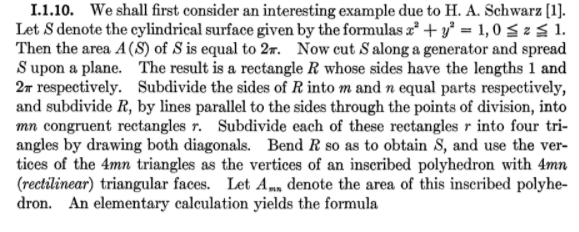
\includegraphics[width=\linewidth]{images/Rado1.png}
\end{image}%
\begin{image}{0.1}{0.8}{0.1}%
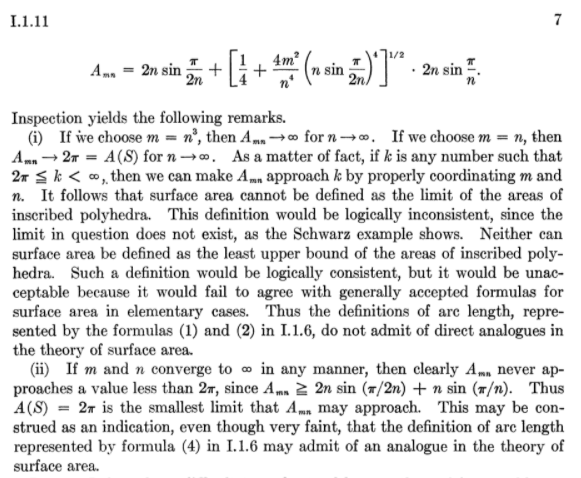
\includegraphics[width=\linewidth]{images/Rado2.png}
\end{image}%
\tcblower
\end{figureptx}%
%
\par
Let's next work out how to compute the area of a patch of a surface lying on an \(m\)-dimensional plane in \(\bbR^{n} (n\ge m)\) as given by a parametric representation via a linear map. Let \(A\) be an \(n\times m\) matrix with rank \(m\) and \(m\le n\). Consider%
\begin{equation*}
F: x \in \mathbb R^m \mapsto Ax \in \mathbb R^n.
\end{equation*}
\(F(\bbR^{m})\)  is an \(m-\)dimensional subspace of \(\mathbb R^n\). Let \(U\) be   the standard cube in \(\mathbb R^m\), then \(F(U)\) is a parallelepiped in \(F(\mathbb R^m)\), with \(\text{ col}_j(A)\), \(j=1,\ldots, m\) as edges.  In the case of \(m=2\) and \(n=3\), \(F(U)\) is a parallelogram with \(\text{ col}_1(A), \text{ col}_2(A)\) as edges and we know that its area can be computed as \(|\text{ col}_1(A)\times \text{ col}_2(A)|\).%
\par
We now develop a formula for higher dimensional settings in the absence of cross product.%
\begin{theorem}{Theorem}{Volume of the Image of a Unit Hypercube under a Linear Map.}{}{theorem-cubeform}%
In the setting above,%
\begin{equation}
\text{ Volume} (F(U)) =\sqrt {\det (A^{\rm T}A)} \text{ Volume}(U).\label{men-eq-cubeform}
\end{equation}
\end{theorem}
\begin{proof}{Proof}{}{proof-cubeform-c}
Choose an orthonormal basis \(\tau_1,\ldots, \tau_m\) of \(F(\mathbb R^m)\), and express each  \(\text{ col}_j(A)\) in terms of this  basis:%
\begin{equation*}
\text{ col}_j(A)=\sum_{i=1}^m B_{ij}\tau_i,
\end{equation*}
and let \(B\) be the \(m\times m\) matrix \((B_{ij})\). Then%
\begin{equation*}
F(\bx) =\sum_{i=1}^m \left( \sum_{j=1}^mB_{ij}x_{j}\right) \tau_i =\left[\tau_1 \cdots \tau_m\right] B\bx
\end{equation*}
so in terms of the basis \(\tau_1,\ldots, \tau_m\), \(F(\bx)\) can be treated as given by \(B\bx\), and \(F(U)\) can be thought of as obtained from the unit cube  in \(F(\mathbb R^m)\) by applying the linear transformation through multiplication by \(B\), and by our earlier discussion%
\begin{equation*}
\text{ Volume} (F(U)) = |\det B | \text{ Volume}(U)=|\det B |.
\end{equation*}
On the other hand, the relations between \(A\) and \(B\) can be written as%
\begin{equation*}
A= \left[\tau_1 \cdots \tau_m\right] B,
\end{equation*}
so%
\begin{equation*}
A^{\rm T}A=B^{\rm T} \left[\tau_1 \cdots \tau_m\right]^{\rm T} \left[\tau_1 \cdots \tau_m \right] B
= B^{\rm T}B,
\end{equation*}
using%
\begin{equation*}
\left[\tau_1 \cdots \tau_m\right]^{\rm T} \left[\tau_1 \cdots \tau_m \right] = I_m.
\end{equation*}
Now it follows that%
\begin{equation*}
|\det B |= \sqrt {\det B \det B^{\rm T}} =  \sqrt {\det (B^{\rm T}B)}= \sqrt {\det (A^{\rm T}A)}
\end{equation*}
(\(B\) is square while \(A\) may not be square, so we can not have \(\det (A^{\rm T}A)=\det (A^{\rm T})\det (A)\)), and we arrive at \hyperref[men-eq-cubeform]{({\xreffont\ref{men-eq-cubeform}})}.\end{proof}
\begin{remark}{Remark}{}{remark-ch_integration-i-d-g}%
Note that the \((i, j)\) entry \(g_{ij}\) of \(A^{\rm T}A\), is \(\text{ col}_i (A) \cdot \text{ col}_j (A)= Ae_i \cdot Ae_j\). This is one of the geometric origins for the Riemannian metric tensor and the appearance of the area (volume) form \(\sqrt {\det (g_{ij})}\, d\bu\).%
\par
After we develop exterior algebra, we will find that%
\begin{equation*}
\text{ col}_1(A)\wedge \text{ col}_2(A)\wedge\cdots\wedge \text{ col}_m(A)=
\left( \det B\right)\, \tau_{1}\wedge \tau_{2}\wedge\cdots\wedge \tau_{m},
\end{equation*}
so \(\det B\) encodes the geometric relation between \(\text{ col}_1(A)\wedge \text{ col}_2(A)\wedge\cdots\wedge \text{ col}_m(A)\) and \(\tau_{1} \, \wedge \tau_{2}\wedge\cdots\wedge \tau_{m}\) formed from two bases of \(F(\bbR^{m})\).%
\end{remark}
\begin{example}{Example}{}{example-ch_integration-i-d-h}%
The area of the parallelogram in \(\bbR^{n}\) with \(\ba =(a_{1},\cdots, a_{n})\) and \(\bb =(b_{1},\cdots, b_{n})\) as its adjacent edges  is given by%
\begin{equation*}
\sqrt{\det \begin{bmatrix} \ba\cdot\ba \amp \ba \cdot \bb \\ \ba\cdot \bb \amp \bb \cdot \bb \end{bmatrix}}.
\end{equation*}
\end{example}
%
%
\typeout{************************************************}
\typeout{Exercises 6.7.2 Exercises}
\typeout{************************************************}
%
\begin{exercises-subsubsection-numberless}{Exercises}{Exercises}{}{Exercises}{}{}{exercises-ch_integration-i-d-i}
\begin{divisionexercise}{1}{}{}{exercise-ch_integration-i-d-i-a}%
Find the area of the subset of the solution set of%
\begin{equation*}
\begin{cases} x_{1} \hphantom{x_{2}}-a x_{3}-c x_{4} \amp =0 \\
\hphantom{x_{2}} x_{2} -b x_{3} - d x_{4} \amp =0\\
\end{cases}
\end{equation*}
which orthogonally projects onto the unit square \(\{(x_{3}, x_{4}): 0\le x_{3}, x_{4}\le 1\}\) in the \(x_{3}\mbox{--}x_{4}\) coordinate plane.%
\end{divisionexercise}%
\begin{divisionexercise}{2}{}{}{exercise-ch_integration-i-d-i-b}%
Find the areas of the triangles with \((1, 0, 0)\) and \((\cos(\frac{\pi}{n}), \pm \sin(\frac{\pi}{n}),\frac{1}{2m})\), and respectively with \((1, 0, 0)\) and \((\cos(\frac{\pi}{n}),  \sin(\frac{\pi}{n}), \pm \frac{1}{2m})\), as vertices.%
\par\smallskip%
\noindent\textbf{\blocktitlefont Answer}.\hypertarget{answer-ch_integration-i-d-i-b-b}{}\quad{}For the former it is \(\frac12\sin(\frac{\pi}{n}) \sqrt{ 4^{2}\sin^{4}(\frac{\pi}{2n})+\frac{1}{m^{2}}}\); for the latter it is \(\frac 1m \sin(\frac{\pi}{2n})\).%
\end{divisionexercise}%
\begin{divisionexercise}{3}{}{}{exercise-ch_integration-i-d-i-c}%
Find the three dimensional volume of the tetrahedron in  \(\bbR^{4}\) with \((1, 0, 0, 0)\), \((0, 1, 0, 0), (0, 0, 1, 0), (0, 0, 0, 1)\) as vertices.%
\par\smallskip%
\noindent\textbf{\blocktitlefont Hint}.\hypertarget{hint-ch_integration-i-d-i-c-b}{}\quad{}The three dimensional volume of a tetrahedron equals \(1/6\) of the volume of a parallelepiped sharing three adjacent edges with the tetrahedron.\end{divisionexercise}%
\end{exercises-subsubsection-numberless}
\end{subsectionptx}
%
%
\typeout{************************************************}
\typeout{Subsection 6.7.3 Volume of an \(m\)-dimensional Differentiable Surface in \(\bbR^{n}\)}
\typeout{************************************************}
%
\begin{subsectionptx}{Subsection}{Volume of an \(m\)-dimensional Differentiable Surface in \(\bbR^{n}\)}{}{Volume of an \(m\)-dimensional Differentiable Surface in \(\bbR^{n}\)}{}{}{subsection-ch_integration-i-e}
Even if \(F\) is not given by a linear map, but is continuously differentiable, and  its Jacobian matrix \(DF(\bu)\) at any \(\bu\) has rank \(m\),  then we can still construct an orthonormal basis  \(\left\{\tau_1(\bu), \cdots, \tau_m(\bu)\right\}\) of \(\text{Span}\left\{D_{1}F(\bu), \ldots, D_{m}F(\bu)\right\}\) (e.g. by the Gram-Schmidt orthogonalization procedure) and write%
\begin{equation*}
DF(\bu)= \left[\tau_1(\bu) \cdots \tau_m(\bu) \right] B(\bu)
\end{equation*}
where  the entries of the \(m\times m\) matrix \(B(\bu )\) are continuous in \(\bu\); furthermore, the above discussion about the role of \(g_{ij}(\bu)
=  D_{i}F(\bu)\cdot D_{j}F(\bu)\) still makes sense. Namely, \(\sqrt{\det (g_{ij}(\bu))}\) is the  ratio of volume of \(DF(\bu)(Q)\) and volume of \(Q\), when Q is a hypercube in the parameter space \(\bbR^{m}\) at \(\bu\), therefore, is the infinitesimal ratio of volume of \(F(Q)\) and volume of \(Q\) when \(Q\) shrinks to \(u\). This leads us to define%
\begin{equation*}
\int_{U} \sqrt{\det (g_{ij}(\bu))}
\end{equation*}
as the \terminology{volume of \(F(U)\)} for any (Jordan-measurable) open domain \(U\) of \(\bbR^{m}\).%
\par
We can use the change of variables formula to check that this definition is independent of the parametrization, namely, if \(\Phi: V\mapsto U\) is a diffeomorphism from \(V\) onto \(U\), then \(\hat F(\bv) = F \circ \Phi (\bv): V \mapsto F(U)\) is another parametrization for \(F(U)\), and we expect%
\begin{equation}
\int_V  \sqrt {\det ({D\hat F}(\bv)^{\rm T} {D\hat F}(\bv))}\; d\bv
=  \int_U  \sqrt {\det (DF(\bu)^{\rm T} DF(\bu))}\; d\bu.\label{men-areainv}
\end{equation}
This follows by using the chain rule%
\begin{equation*}
D{\hat F}(\bv) = DF(\Phi(\bv)) D\Phi (\bv),
\end{equation*}
which leads to%
\begin{equation}
D{\hat F}(\bv)^{\rm T}D{\hat F}(\bv)=D\Phi(\bv)^{\rm T} DF(\Phi(\bv))^{\rm T}DF(\Phi(\bv)) D\Phi (\bv).\label{men-eq-metricform}
\end{equation}
Since \(D\Phi(\bv)^{\rm T}  \), \(DF(\Phi(\bv))^{\rm T}  DF(\Phi(v))\), and \(D\Phi (v)\) are all \(m\times m\) square matrices, so%
\begin{align*}
\det (D{\hat F}(\bv)^{\rm T}D{\hat F}(\bv))
\amp =\det D\Phi(\bv)^{\rm T}  \det ( DF(\Phi(\bv))^{\rm T}DF(\Phi(\bv)) ) \det D\Phi (\bv)\\
\amp= \det ( DF(\Phi(\bv))^{\rm T}DF(\Phi(\bv)) ) |\det D\Phi (\bv) |^{2}.
\end{align*}
This results in%
\begin{equation}
\sqrt{\det (D{\hat F}(\bv)^{\rm T}D{\hat F}(\bv))}
=\sqrt{\det ( DF(\Phi(\bv))^{\rm T}DF(\Phi(\bv)) )} |\det D\Phi (\bv)|,\label{men-eq-volumeform}
\end{equation}
which, when applied to the left hand side of \hyperref[men-areainv]{({\xreffont\ref{men-areainv}})} in making the change of variables \(\bu=\Phi(\bv)\), confirms \hyperref[men-areainv]{({\xreffont\ref{men-areainv}})}.%
\begin{remark}{Remark}{}{remark-ch_integration-i-e-d}%
The computations above indicate that, if we accept the formal relation \(d\bu = |\det D\Phi (\bv)| d\bv\) in the sense of change of variables in integration, then%
\begin{equation*}
\sqrt {\det ({D\hat F}(\bv)^{\rm T} {D\hat F}(\bv))}\; d\bv
=  \sqrt {\det (DF(\bu)^{\rm T} DF(\bu))}\; d\bu
\end{equation*}
is a geometric quantity independent of the parametrization, and is called the \terminology{volume (area) form} of the submanifold (surface) \(F(U)\), and denoted by \(d \text{vol}\) or \(d A\).%
\par
Note also that if we define \(\hat g_{ij}(\bv)=D_{i}\hat F(\bv)\cdot D_{j}\hat F(\bv)\), then it is the \((i, j)\) entry of \({D\hat F}(\bv)^{\rm T} {D\hat F}(\bv))\), and the relations above  \hyperref[men-eq-metricform]{({\xreffont\ref{men-eq-metricform}})} and \hyperref[men-eq-volumeform]{({\xreffont\ref{men-eq-volumeform}})} become%
\begin{equation*}
(\hat g_{ij}(\bv))=D\Phi(\bv)^{\rm T} (g_{ij}(\Phi(\bv))) D\Phi(\bv)
\text{ and }  \sqrt{\det (\hat g_{ij}(\bv))}\, d\bv = \sqrt{\det (g_{ij}(\bu))}\, d\bu.
\end{equation*}
%
\par
The \(\hat g_{ij}(\bv)\) and \(g_{ij}(\bu)\) here are obtained through \(D\hat F(\bv)\) and \(DF(\bu)\) respectively. There are other ways of obtaining such functions consisting of positive definite matrices associated with different parametrization and satisfying the above relations \hyperref[men-eq-metricform]{({\xreffont\ref{men-eq-metricform}})} and \hyperref[men-eq-volumeform]{({\xreffont\ref{men-eq-volumeform}})}. Once we have them we can use them to define the volume of a region and the integral of a function just as above. The \(\hat g_{ij}(\bv)\) and \(g_{ij}(\bu)\) turn out to be the coordinate representations of a \terminology{Riemannian metric}.%
\end{remark}
In the case of \(m=2\) and \(n=3\),%
\begin{equation*}
g_{11}=D_{1}F\cdot D_{1}F, g_{12}=D_{1}F\cdot D_{2}F, 
g_{22}=D_{2}F\cdot D_{2}F,
\end{equation*}
and we know from the properties of cross product and dot product for three dimensional vectors that%
\begin{equation*}
|D_{1}F\times D_{2}F|=\sqrt{\det (g_{ij})}
\end{equation*}
in this case.%
\begin{example}{Example}{}{example-ch_integration-i-e-f}%
Suppose that \(U\) is a Jordan measurable open domain in \(\bbR^{n}\), \(f(\bx)\in \bbR\) has continuous and bounded partial derivatives in \(U\). Then the graph of \(f\) over \(U\) has the representation \(G(\bx)=(\bx, f(\bx))\) with \(D_{i}G(\bx)=(\be_{i}, D_{i}f(\bx))\), so \(g_{ii}=1+|D_{i}f(\bx)|^{2}\) and \(g_{ij}=D_{i}f(\bx) D_{j}f(\bx)\) for \(i\ne j\). To find \(\det (g_{ij}(\bx))\), note that \((g_{ij}(\bx))=I +[Df(\bx)][Df(\bx)]^{\mathrm t}\), which has eigenvalues \(1\) with multiplicity \(n-1\) and \(1+|Df(\bx)|^{2}\) with multiplicity \(1\), so \(\det (g_{ij}(\bx))= 1+|Df(\bx)|^{2}\) and the \(n\)-dimensional volume of the graph of \(f\) over \(U\) is given  by%
\begin{equation*}
\int_{U} \sqrt{1+|Df(\bx)|^{2}}\, d\bx.
\end{equation*}
%
\par
The requirement that \(f(\bx)\) has continuous and bounded partial derivatives in \(U\) can be relaxed when the integral above can be treated as an appropriate improper integral, such as in the case of the area of a hemisphere when represented as a graph.%
\end{example}
\begin{example}{Example}{}{example-ch_integration-i-e-g}%
The  sphere \(x^{2}+y^{2}+z^{2}=R^{2}\) in \(\bbR^{3}\) is circumscribed by the round cylinder \(x^{2}+y^{2}=R^{2}\). Both have parametric representation in terms of cylindrical coordinates, with the former given by%
\begin{equation*}
S(\theta, z)=(\sqrt{R^{2}-z^{2}} \cos\theta, \sqrt{R^{2}-z^{2}} \sin \theta, z), 0\le \theta \lt 2\pi, -R\le z \le R,
\end{equation*}
and the latter by%
\begin{equation*}
C(\theta, z)=(R\cos \theta, R\sin\theta, z), 0\le \theta \lt 2\pi, z\in \bbR.
\end{equation*}
Note that%
\begin{equation*}
D_{\theta}S(\theta, z)\cdot D_{z}S(\theta, z)=0, \Vert D_{\theta}S(\theta, z)\Vert =\sqrt{R^{2}-z^{2}},
\Vert D_{z}S(\theta, z)\Vert=\frac{R}{\sqrt{R^{2}-z^{2}}},
\end{equation*}
so the area of the section of the sphere for \(0\le \theta \lt 2\pi, -R\le z_{1}\le z \le z_{2}\le R\) is given by%
\begin{align*}
\amp \int_{0}^{2\pi} \int_{z_{1}}^{z_{2}} \sqrt{\det \begin{bmatrix} D_{\theta}S(\theta, z)\cdot D_{\theta}S(\theta, z) \amp
D_{\theta}S(\theta, z) \cdot D_{z}S(\theta, z) \\ D_{\theta}S(\theta, z) \cdot D_{z}S(\theta, z) \amp
D_{z}S(\theta, z) \cdot D_{z}S(\theta, z) \end{bmatrix}}\ dz\, d\theta\\
= \amp \int_{0}^{2\pi} \int_{z_{1}}^{z_{2}} R \ dz\, d\theta, 
\end{align*}
while%
\begin{equation*}
D_{\theta}C(\theta, z)\cdot D_{z}C(\theta, z)=0, \Vert D_{\theta}C(\theta, z)\Vert =R,
\Vert D_{z}C(\theta, z)\Vert=1,
\end{equation*}
so the area of the section of the cylinder for \(0\le \theta \lt 2\pi, z_{1}\le z \le z_{2}\) is given by%
\begin{align*}
\amp \int_{0}^{2\pi} \int_{z_{1}}^{z_{2}} \sqrt{\det \begin{bmatrix} D_{\theta}C(\theta, z)\cdot D_{\theta}C(\theta, z) \amp
D_{\theta}C(\theta, z) \cdot D_{z}C(\theta, z) \\ D_{\theta}C(\theta, z) \cdot D_{z}C(\theta, z) \amp
D_{z}C(\theta, z) \cdot D_{z}C(\theta, z) \end{bmatrix}}\ dz\, d\theta \\
= \amp \int_{0}^{2\pi} \int_{z_{1}}^{z_{2}} R \ dz\, d\theta. 
\end{align*}
The areas of these two sections are equal for any \(-R\le z_{1} \lt z_{2}\le R\), which was first discovered by Archimedes. In particular, the area of the sphere is \(\int_{0}^{2\pi} \int_{-R}^{R} R \ dz\, d\theta=4\pi R^{2}\).%
\par
One could represent the upper hemisphere	as a graph \(z=g(x, y)=\sqrt{R^{2}-x^{2}-y^{2}}\) and use the integration of \(\sqrt{1+|Dz|^{2}}\) over \(x^{2}+y^{2}\lt R\) to compute its area, but \(|Dz|\) becomes unbounded as \(x^{2}+y^{2}\to R^{2}\), so one has to deal with that issue. In the case here one needs to evaluate the improper integral \(\int_{x^{2}+y^{2} \lt R^{2}} \frac{R}{\sqrt{R^{2}-x^{2}-y^{2}}}\, dx dy\), which can be converted into an improper integral in polar coordinate as \(\int_{0}^{2\pi} \int_{0}^{R}\frac{Rr}{\sqrt{R^{2}-r^{2}}}\, dr d\theta\).%
\end{example}
%
%
\typeout{************************************************}
\typeout{Exercises 6.7.3 Exercises}
\typeout{************************************************}
%
\begin{exercises-subsubsection-numberless}{Exercises}{Exercises}{}{Exercises}{}{}{exercises-ch_integration-i-e-h}
\begin{divisionexercise}{1}{}{}{exercise-ch_integration-i-e-h-a}%
Find the area of the region of the plane \(x+y+z=1\) enclosed within the cylinder \(x^2+y^2 \le 1\).%
\end{divisionexercise}%
\begin{divisionexercise}{2}{}{}{exercise-ch_integration-i-e-h-b}%
Find the area of the cylinder \(x^{2} +y^{2}=1\) intersected between the planes \(x+y+z=\pm 1\).%
\end{divisionexercise}%
\begin{divisionexercise}{3}{}{}{exercise-ch_integration-i-e-h-c}%
Find the three dimensional volume of the sphere \(x_{1}^{2}+x_{2}^{2}+x_{3}^{2}+x_{4}^{2}=R^{2}\) in \(\bbR^{4}\) by (i) treating it as the union of two graphs \(x_{4}=\pm \sqrt{R^{2}-x_{1}^{2}-x_{2}^{2}-x_{3}^{2}}\) and evaluating an integral in \(x_{1}^{2}+x_{2}^{2}+x_{3}^{2}\le R^{2}\), and (ii) using the parametric representation in spherical polar coordinates%
\begin{equation*}
\begin{cases} x_{1} \amp = R\sin\theta_{2}\sin\theta_{1}\cos\phi \\
x_{2} \amp = R\sin\theta_{2}\sin\theta_{1}\sin\phi \\
x_{3} \amp = R\sin\theta_{2}\cos\theta_{1} \\
x_{4} \amp = R\cos\theta_{2}\\
\end{cases}
\end{equation*}
for \(0\le \theta_{1}, \theta_{2}\le \pi, 0\le \phi \le 2\pi\).%
\par\smallskip%
\noindent\textbf{\blocktitlefont Hint}.\hypertarget{hint-ch_integration-i-e-h-c-b}{}\quad{}For (i), after a change of variables into spherical polar coordinates, it reduces to \(4\pi R^{3} \left( \int_{0}^{1}\frac{\rho^{2}}{\sqrt{1-\rho^{2}}}\, d\rho \right)\);  for (ii), observe that the column vectors of the Jacobian matrix are orthogonal to each other.\end{divisionexercise}%
\begin{divisionexercise}{4}{}{}{exercise-ch_integration-i-e-h-d}%
Let \(r=r(z) >0\) be continuously differentiable on \([a, b]\). Then it generates a surface of revolution via the parametrization%
\begin{equation*}
(z, \theta)\mapsto (r(z)\cos\theta, r(z)\sin\theta, z) \in \bbR^{3}, a\le z \le b, 0\le \theta \le 2\pi.
\end{equation*}
Verify that the area of this surface is given by%
\begin{equation*}
2\pi \int_{a}^{b} r(z) \sqrt{(r'(z))^{2}+1}\, dz.
\end{equation*}
%
\par
\(r_{1}(z)=\cosh (z)\) and \(r_{2}(z)=\cosh (1)\) for \(|z|\le 1\) both can be used to generate a surface of revolution sharing the boundary \((\cosh(1)\cos(\theta), \cosh(1)\sin(\theta), \pm 1)\). which of them has less area?%
\end{divisionexercise}%
\begin{divisionexercise}{5}{}{}{exercise-ch_integration-i-e-h-e}%
Check whether Archimedes' observation about the area of the portion of a sphere between two parallel planes equal the area  of the circumscribed cylinder between the same parallel planes holds in \(\bbR^{n}\) for \(m > 3\). Namely, compare the area of the portion of the sphere \(x_{1}^{2}+\cdots+x_{n}^{2}=R^{2}\) between \(z_{1}\le x_{n}\le z_{2}\) and that of \(x_{1}^{2}+\cdots+x_{n-1}^{2}=R^{2}\), \(z_{1}\le x_{n}\le z_{2}\), for a general \(n\).%
\end{divisionexercise}%
\end{exercises-subsubsection-numberless}
\end{subsectionptx}
%
%
\typeout{************************************************}
\typeout{Subsection 6.7.4 The integral of a Function on an \(m\)-dimensional Differentiable Surface in \(\bbR^{n}\)}
\typeout{************************************************}
%
\begin{subsectionptx}{Subsection}{The integral of a Function on an \(m\)-dimensional Differentiable Surface in \(\bbR^{n}\)}{}{The integral of a Function on an \(m\)-dimensional Differentiable Surface in \(\bbR^{n}\)}{}{}{subsection-ch_integration-i-f}
Suppose that \(\bu \in U\subset \bbR^{m}\mapsto F(\bu)\in \bbR^{n}\) is a parametrization for a surface patch \(F(U)\) and \(f(\bx)\) is a  function defined in a set in \(\bbR^{n}\) which includes \(F(U)\), then it is reasonable to define the \terminology{integral of \(f\) on \(F(U)\)} by%
\begin{align*}
\int_{F(U)}f(\bx)\, d \text{vol}= \amp \int_{U} f(F(\bu)) \sqrt {\det (DF(\bu)^{\rm T} DF(\bu))}\, d\bu\\
=\amp
\int_{U} f(F(\bu)) \sqrt {\det (g_{ij}(\bu))}\, d\bu
\end{align*}
when this integral exists.%
\par
An analogous discussion as above shows that this definition is independent of the parametrization used. Thus we have reduced the integration of a function on a surface to the integration on a domain in the Euclidean space of a modified integrand. As a result, the usual properties of integrals such as the linearity in the integrand hold.%
\begin{example}{Example}{}{example-ch_integration-i-f-d}%
For any continuous function \(f(x, y, z)\) defined on the sphere \(S_{R}: x^{2}+y^{2}+z^{2}=R^{2}\) in \(\bbR^{3}\), using cylindrical representation, its integral on \(S_{R}\), \(\int_{S_{R}} f(x, y, z) dA\) is given by%
\begin{equation*}
\int_{0}^{2\pi}\int_{-R}^{R} f(\sqrt{R^{2}-z^{2}} \cos\theta, \sqrt{R^{2}-z^{2}} \sin\theta, z) R \ dz\, d\theta\text{.}
\end{equation*}
For example,%
\begin{equation*}
\int_{S_{R}} x^{2} dA =\int_{0}^{2\pi}\int_{-R}^{R} (R^{2}-z^{2}) \cos^{2}\theta R \ dz\, d\theta.
\end{equation*}
But this integral could also be evaluated using the symmetry of the sphere%
\begin{equation*}
\int_{S_{R}} x^{2} dA=\int_{S_{R}} x^{2} dA=\int_{S_{R}} x^{2} dA=\int_{S_{R}} \frac{x^{2}+y^{2}+z^{2}}{3} dA
=\frac{4R^{4}\pi}{3}.
\end{equation*}
\end{example}
%
%
\typeout{************************************************}
\typeout{Exercises 6.7.4 Exercises}
\typeout{************************************************}
%
\begin{exercises-subsubsection-numberless}{Exercises}{Exercises}{}{Exercises}{}{}{exercises-ch_integration-i-f-e}
\begin{divisionexercise}{1}{}{}{exercise-ch_integration-i-f-e-a}%
Evaluate \(\int_{x^{2}+y^{2}=R^{2}, |z|\le h} x^{2}\, dA\).%
\end{divisionexercise}%
\begin{divisionexercise}{2}{}{}{exercise-ch_integration-i-f-e-b}%
Evaluate the integral \(\int_{S}  z \, dA\), where \(S\) is the region of the plane \(x+y+z=1\) enclosed within the cylinder \(x^2+y^2 \le 1\).%
\end{divisionexercise}%
\begin{divisionexercise}{3}{}{}{exercise-ch_integration-i-f-e-c}%
Evaluate the integral \(\int_{S}  z^{2} \, dA\), where \(S\) is the cylinder \(x^{2} +y^{2}=1\) intersected between the planes \(x+y+z=\pm 1\).%
\end{divisionexercise}%
\begin{divisionexercise}{4}{}{}{exercise-ch_integration-i-f-e-d}%
In the setting of \hyperref[exercise-ex-foliation]{Exercise~{\xreffont\ref{exercise-ex-foliation}}}, suppose that \(h(\bx)\) is integrable in \(V\), the integral \(\int_{V} h(\bx) \, d\bx\) can be evaluated using the parametrization \(G: (\bx',t)\in  B(\mathbf 0, r) \times (-\delta, \delta) \mapsto (\bx', g(\bx', t))\in V\). Let \(g_{ij}(\bx', t) = D_{i}G(\bx', t)\cdot D_{j} G(\bx', t)\), where we interpret \(D_{n}\) as \(D_{t}\).%
%
\begin{enumerate}[label=(\alph*)]
\item{}Verify that \(\sqrt{\det(g_{ij}(\bx', t))}=\vert \partial_{t} g(\bx', t)\vert\).%
\item{}Verify that%
\begin{equation*}
\vert \partial_{t} g(\bx', t)\vert \Vert D f(\bx', g(\bx', t)) \Vert 
=\sqrt{1+\sum_{i=1}^{n-1}\vert \partial_{i}g(\bx', t)\vert^{2}}\text{.}
\end{equation*}
%
\item{}Show that%
\begin{align*}
\int_{V} h(\bx) \, d\bx=\amp \int_{- \delta}^{\delta} \int_{B(\mathbf 0, r)} h(\bx', g(\bx', t)) 
\vert \partial_{t} g(\bx', t)\vert \, d\bx' dt \\
=\amp \int_{- \delta}^{\delta} \int_{B(\mathbf 0, r)} \frac{h(\bx', g(\bx', t))}{\Vert D f(\bx', g(\bx', t)) \Vert}
\sqrt{1+\sum_{i=1}^{n-1}\vert \partial_{i}g(\bx', t)\vert^{2}} \, d\bx' dt. 
\end{align*}
%
\end{enumerate}
Note that the integral%
\begin{equation*}
\int_{B(\mathbf 0, r)} \frac{h(\bx', g(\bx', t))}{\Vert D f(\bx', g(\bx', t)) \Vert}
\sqrt{1+\sum_{i=1}^{n-1}\vert \partial_{i}g(\bx', t)\vert^{2}} \, d\bx'
=\int_{V\cap \{f =t\}} \frac{h(\bx)}{\Vert D f(\bx) \Vert} \, d A
\end{equation*}
is an integral on the leaf \(V\cap \{f =t\}\).  This evaluation of the integral in terms of integrals on the leaves of level surfaces of some function is called \terminology{co-area formula}.%
\par
Here is a simple application of the co-area formula. To evaluate \(\int_{x^{2}+y^{2}+z^{2}\le R^{2}} h(x, y, z)\, dx\, dy\, dz\), we can choose \(f(x, y, z)=\sqrt{x^{2}+y^{2}+z^{2}}\). Then the set \(\{(x, y, z): x^{2}+y^{2}+z^{2}\le R^{2}\}\) can be described as \(\{(x, y, z): 0\le f(x, y, z) \le R\}\). Note that \(\Vert Df(x, y, z)\Vert=1\). Despite that \(f(x, y, z)\) fails to be differentiable at \((x, y, z)=(0, 0, 0)\), we can still argue that%
\begin{equation*}
\int_{x^{2}+y^{2}+z^{2}\le R^{2}} h(x, y, z)\, dx\, dy\, dz
=\int_{0}^{R} \left( \int_{x^{2}+y^{2}+z^{2}=r^{2}} h(x, y, z)\, dA\right)\, dr.
\end{equation*}
%
\end{divisionexercise}%
\end{exercises-subsubsection-numberless}
\end{subsectionptx}
\end{sectionptx}
\end{chapterptx}
%
%
\typeout{************************************************}
\typeout{Chapter 7 Exterior Differential Calculus and Integration of Differential Forms}
\typeout{************************************************}
%
\begin{chapterptx}{Chapter}{Exterior Differential Calculus and Integration of Differential Forms}{}{Exterior Differential Calculus}{}{}{chapter-Math412-Notes-j}
\renewcommand*{\chaptername}{Chapter}
\begin{introduction}{}%
Our next objective is to extend the notion of the curl and divergence of a vector field introduced in multi-variable calculus and the Green Theorem, the Stokes Theorem, and the Divergence Theorem to more general contexts.\end{introduction}%
%
%
\typeout{************************************************}
\typeout{Section 7.1 A Brief Review of the Notion of Curl and Divergence of a Vector Field}
\typeout{************************************************}
%
\begin{sectionptx}{Section}{A Brief Review of the Notion of Curl and Divergence of a Vector Field}{}{A Brief Review of the Notion of Curl and Divergence of a Vector Field}{}{}{section-Math412-Notes-j-d}
In multi-variable calculus the line integral of a vector field \(\vec{X}=(X_{1}(\bx),\cdots, X_{n}(\bx)), n=2 \text{ or } 3,\) along a path (or loop) \(\Gamma: t\in [a, b]\mapsto \vec{r}(t)\),  is defined as%
\begin{equation*}
\int_{\Gamma} \vec{X}\cdot d\vec{r} = \int_{a}^{b} 
\left( X_1(\vec{r}(t))r_1'(t)+ \cdots + X_n(\vec{r}(t))r_n'(t)\right)dt,
\end{equation*}
and the flux of \(\vec{X}\) across a surface \(S\), is defined as%
\begin{equation*}
\int_S \vec{X} \cdot \vec{n}\, dA,
\end{equation*}
where \(\vec{n}(\bx)\) is a (continuous) choice of unit normal vector to \(S\) at \(\bx\). In both cases, the integrand is not a given scalar function but a bilinear function of a given vector field and of a tangent vector of the curve or a normal vector of the surface.%
\par
One natural question is \emph{what infinitesimal quantities measure the "strength" of  the circulation of the vector field along a closed loop or flux of the vector field across a closed surface near a point?} The answers turn out to be the \terminology{curl} and, respectively, \terminology{divergence} of the vector field \(\vec{X}\) at the point.%
\par
For \(n=3\), the curl of \(\vec{X}=(X_{1}(\bx),X_{2}(\bx), X_{3}(\bx))\) at \(\bx\) is the vector%
\begin{equation*}
\text{curl} \vec{X}(\bx)=
(\frac{\partial X_3}{\partial x_2}-\frac{\partial X_2}{\partial x_3},
\frac{\partial X_1}{\partial x_3}-\frac{\partial X_3}{\partial x_1},
\frac{\partial X_2}{\partial x_1}-\frac{\partial X_1}{\partial x_2}).
\end{equation*}
For \(n=2\), we can treat \(\vec{X}\) as a special case of \(n=3\) with \(X_{3}(\bx)=0\) and \(X_{i}(\bx)\) for \(i=1, 2\) depend only on \((x_{1}, x_{2})\), so the curl of such a vector field takes the form of%
\begin{equation*}
(0, 0, \frac{\partial X_2}{\partial x_1}-\frac{\partial X_1}{\partial x_2}).
\end{equation*}
The divergence of \(\vec{X}=(X_{1}(\bx), X_{2}(\bx), X_{3}(\bx))\) is the scalar function%
\begin{equation*}
\text{div}\vec{X}(\bx)= \sum_{j=1}^{3} \frac{\partial X_j(\bx)}{\partial x_j}.
\end{equation*}
%
\par
The Stokes Theorem says that if \(\Gamma: t\in [a, b]\mapsto \vec{r}(t)\) is a differentiable closed loop (meaning \(\Gamma(a)=\Gamma(b)\)) in \(\bbR^{3}\) and spans a differentiable surface \(S\), then%
\begin{equation*}
\int_{\Gamma} \vec{X}\cdot d\vec{r} = \int_S \text{curl}\vec{X}(\bx) \cdot \vec{n}(\bx)\, dA,
\end{equation*}
where \(\vec{n}(\bx)\) is an appropriately chosen unit normal vector field to \(S\).%
\par
If we accept Stokes Theorem, it can be used to give some geometric interpretation for \(\text{curl}\vec{X}\).  Fix some \(\bx_{0}\) and a plane \(\Pi\) containing \(\bx_{0}\) with a unit normal vector \(\vec{n}\). Take \(S\) to be the disc in the plane \(\Pi\) of radius \(\epsilon >0\) centered at \(\bx_{0}\) and \(\Gamma\) to be the boundary of this disc. Then%
\begin{equation*}
\lim_{\epsilon \to 0} \frac{1}{\pi \epsilon^{2}} \int_{\Gamma} \vec{X}\cdot d\vec{r}=
\lim_{\epsilon \to 0} \frac{1}{\pi \epsilon^{2}} \int_S \text{curl}\vec{X}(\bx) \cdot \vec{n}(\bx)\, dA
=\text{curl}\vec{X}(\bx_{0}) \cdot \vec{n}.
\end{equation*}
Thus \(\text{curl}\vec{X}(\bx_{0}) \cdot \vec{n}\) is the infinitesimal rate of circulation\(\mbox{---}\)circulation per unit area\(\mbox{---}\)of \(\vec{X}\) along closed loops surrounding \(\bx_{0}\) in the plane through \(\bx_{0}\) with unit normal \(\vec{n}\).%
\par
In fact, we can see why \(\text{curl}\vec{X}\) is defined this way by examining%
\begin{equation*}
\lim_{\epsilon \to 0} \frac{1}{\pi \epsilon^{2}} \int_{\Gamma} \vec{X}\cdot d\vec{r}
\end{equation*}
without the knowledge of Stokes Theorem. We will see  that, if the vector field \(\vec{X}\) is differentiable at \(\bx_{0}\), then  this limit exists and is given by the expression above.%
\par
In the simple setting of the two dimensional plane, if \(\vec{X}\) is continuously differentiable in a neighborhood of \({\mathbf x}_{0}=(x_{0}, y_{0})\), and we take \(\Gamma\) to be a small square loop of side length \(2\epsilon\) around \({\mathbf x}_{0}\), then%
\begin{align*}
\amp \int_{\Gamma} \vec{X}\cdot d\vec{r} \\
= \amp
\int_{x_{0}-\epsilon}^{x_{0}+\epsilon} \left\{X_{1}(x, y_{0}-\epsilon)- X_{1}(x, y_{0}+\epsilon)\right\}\, dx
+ \int_{y_{0}-\epsilon}^{y_{0}+\epsilon} \left\{X_{2}(x_{0}+\epsilon, y)-X_{2}(x_{0}-\epsilon, y)\right\}\, dy\\
= \amp 
\int_{x_{0}-\epsilon}^{x_{0}+\epsilon} \int_{y_{0}-\epsilon}^{y_{0}+\epsilon} 
- \frac{\partial X_{1}(x, y)}{\partial y} \, dy dx +
\int_{y_{0}-\epsilon}^{y_{0}+\epsilon} \int_{x_{0}-\epsilon}^{x_{0}+\epsilon} 
\frac{\partial X_{2}(x, y)}{\partial x} \, dx dy\\
= \amp \int_{[x_{0}-\epsilon, x_{0}+\epsilon] \times [y_{0}-\epsilon, y_{0}+\epsilon]}
\left\{  \frac{\partial X_{2}(x, y)}{\partial x}- \frac{\partial X_{1}(x, y)}{\partial y}\right\}\, dx dy.
\end{align*}
This is the simplest form of Green's theorem and motivates the definition of the curl of a two dimensional vector field \((X_{1}(x, y), X_{2}(x, y))\) as \(\frac{\partial X_{2}(x, y)}{\partial x}- \frac{\partial X_{1}(x, y)}{\partial y}\). Note that at any point \({\mathbf x}_{0}=(x_{0}, y_{0})\), its value is determined as%
\begin{equation*}
\lim_{\epsilon\to 0}\frac{1}{\text{Area enclosed by } \Gamma} \int_{\Gamma} \vec{X}\cdot d\vec{r}.
\end{equation*}
%
\par
In three dimension or higher, the simplest loops are planar ones, namely, a loop contained in the plane spanned by  a pair of orthonormal vectors \(\vec{\xi}\) and \(\vec{\eta}\) -{}-{}- we take \({\mathbf x}_{0}\) to be the origin for simplicity, and \(\Gamma: t\mapsto \vec{\gamma}(t)\) be a closed loop near and enclosing \({\mathbf x}_{0}\) in the plane spanned by \(\vec{\xi}\) and \(\vec{\eta}\)  given as%
\begin{equation*}
\vec{\gamma}(t)=x(t)\vec{\xi} + y(t)\vec{\eta}.
\end{equation*}
Assuming \(\vec{X}\) to have the necessary differentiability, then Taylor expansion%
\begin{equation*}
\vec{X}(\vec{\gamma}(t))= \vec{X}({\mathbf x}_{0})+
\left[\frac{\partial \vec{X}}{\partial {\mathbf x}}({\mathbf x}_{0})\right]( \vec{\gamma}(t)- {\mathbf x}_{0})+ 
h.o.t.\ (\Vert \vec{\gamma}(t)- {\mathbf x}_{0}\Vert )
\end{equation*}
gives the leading order term of \(\int_{\Gamma} \vec{X}\cdot d\vec{r}\) to be%
\begin{align*}
\amp \sum_{i,j} \frac{\partial X_i({\mathbf x}_0)}{\partial x_j} \int_{\Gamma} \left(x(t)\xi_j + y(t)\eta_j\right)
\left(x'(t)\xi_i +y'(t)\eta_i\right)dt \\
= \amp \sum_{i,j} \frac{\partial X_i({\mathbf x}_0)}{\partial x_j} \int_{\Gamma} \left(x(t)x'(t)\xi_i\xi_j +
y(t)y'(t)\eta_i\eta_j + x(t)y'(t)\xi_j\eta_i +y(t)x'(t)\xi_i\eta_j\right)dt\\
= \amp \sum_{i,j} \frac{\partial X_i({\mathbf x}_0)}{\partial x_j}\left(\xi_j\eta_i \int_{\Gamma} x(t)y'(t)dt + 
\xi_i\eta_j  \int_{\Gamma} y(t)x'(t) dt\right)
\end{align*}
where we have used that along any closed loop%
\begin{equation*}
\int_{\Gamma} \vec{X}({\mathbf x}_{0})\cdot \vec{\gamma}'(t)\, dt=
\int_{\Gamma} \left[\frac{\partial \vec{X}}{\partial {\mathbf x}}({\mathbf x}_{0})\right] {\mathbf x}_{0}\cdot 
\vec{\gamma}'(t)\, dt=0,
\end{equation*}
and%
\begin{equation*}
\int_{\Gamma} x(t)x'(t) dt = \int_{\Gamma}  y(t)y'(t) dt =0,
\end{equation*}
but%
\begin{equation*}
\int_{\Gamma} x(t)y'(t)dt = -  \int_{\Gamma} y(t)x'(t) dt
\end{equation*}
equals the area enclosed by \(\Gamma\) -{}-{}- one may take \(\Gamma\) to be a square or circle loop to see this, so the leading order term of \(\int_{\Gamma} \vec{X}\cdot d\vec{r}\) is%
\begin{equation*}
\sum_{i,j} \frac{\partial X_i({\mathbf x}_{0})}{\partial x_j} \left(\xi_j\eta_i - \xi_i\eta_j  \right)\cdot
\left(\mbox{Area enclosed by } \Gamma \right).
\end{equation*}
In other words,%
\begin{equation*}
\lim_{\epsilon\to 0}\frac{1}{\text{Area enclosed by } \Gamma} \int_{\Gamma} \vec{X}\cdot d\vec{r}
=\sum_{i,j} \frac{\partial X_i({\mathbf x}_{0})}{\partial x_j} \left(\xi_j\eta_i - \xi_i\eta_j  \right).
\end{equation*}
%
\par
This derivation works for any dimension \(n\). We observe that this "infinitesimal strength" of circulation of \(\vec{X}\) along loops near \({\mathbf x}_{0}\) depends on the above specific combinations of derivatives of  \(\vec{X}\) as well as on the plane in terms of a choice of an orthonormal basis; and the dependence on these derivatives of  \(\vec{X}\) and on  \(\vec{\xi}\) and \(\vec{\eta}\) is linear in each when the remaining variables are held as constant\(\mbox{ ---}\)this is the notion of a \terminology{multi-linear} function; here, we momentarily relax the condition that \(\vec{\xi}\) and \(\vec{\eta}\) are orthonormal and allow them to be any pair of vectors.  Furthermore,  the dependence on \((\vec{\xi}, \vec{\eta})\) is antisymmetrical in \((\vec{\xi}, \vec{\eta})\), and if \(\vec{\xi}'\) and \(\vec{\eta}'\) are another pair of vectors such that \(\text{Span}\{ \vec{\xi}',\vec{\eta}'\} = \text{Span}\{ \vec{\xi},\vec{\eta}\}\), then the quantities \(\xi_j'\eta_i' - \xi_i'\eta_j' \) and \(\xi_j\eta_i - \xi_i\eta_j \) have a common proportionality constant equal to the determinant of the matrix that relates the two pairs of bases and equal \(\pm 1\) when both bases are orthonormal.%
\begin{inlineexercise}{Exercise}{}{exercise-exe-extprod}%
Verify that if \([\vec{\xi}',\vec{\eta}']=[\vec{\xi},\vec{\eta}]A\) for some \(2\times 2\) matrix \(A\), then \(\xi_j'\eta_i' - \xi_i'\eta_j'=(\det A)(\xi_j\eta_i - \xi_i\eta_j) \), and that if \(\{ \vec{\xi}',\vec{\eta}'\}\) and \(\{ \vec{\xi},\vec{\eta}\}\) are orthonormal, then \(A\) is an orthogonal matrix.%
\end{inlineexercise}%
In the case of dimension \(3\), if we take%
\begin{equation*}
\vec{n}=\vec{\xi}\wedge\vec{\eta}=(\xi_2\eta_3-\xi_3\eta_2, \xi_3\eta_1-\xi_1\eta_3, \xi_1\eta_2-\xi_2\eta_1),
\end{equation*}
then it is a unit normal to the plane spanned by \(\vec{\xi}\) and \(\vec{\eta}\), and%
\begin{align*}
\amp \sum_{i,j} \frac{\partial X_i}{\partial x_j} ({\mathbf x}_{0})
\left(\xi_j\eta_i - \xi_i\eta_j  \right)\\
=\amp (\frac{\partial X_3}{\partial x_2}-\frac{\partial X_2}{\partial x_3},
\frac{\partial X_1}{\partial x_3}-\frac{\partial X_3}{\partial x_1},
\frac{\partial X_2}{\partial x_1}-\frac{\partial X_1}{\partial x_2})\cdot \vec{n},
\end{align*}
thus producing the concept of the \emph{curl} of a vector field in dimension \(3\).%
\par
In the general dimension, using exterior algebra motivated by the above discussion and to be introduced soon, we see that \(\xi_j\eta_i - \xi_i\eta_j\) are simply the components of \(\vec{\xi}\wedge \vec{\eta}\), and%
\begin{equation*}
(\vec{\xi}, \vec{\eta}) \mapsto \sum_{i,j} \frac{\partial X_i}{\partial x_j}({\mathbf x}_{0}) 
\left(\xi_j\eta_i - \xi_i\eta_j  \right)
\end{equation*}
is a bilinear antisymmetric function on \((\vec{\xi}, \vec{\eta})\) (we may remove the orthonormal condition on \(\vec{\xi}, \vec{\eta}\) now).%
\par
For any \(i \lt j\), the coefficient of \((\xi_i\eta_j - \xi_j\eta_i)\) above is \(\frac{\partial X_j}{\partial x_i}- \frac{\partial X_i}{\partial x_j}\). Thus the natural generalization of the notion of the curl of a vector field \(\vec{X}\) in \(\bbR^{n}, n>3\), is not a vector field, but an object that acts on any pair of vectors in a bilinear and antisymmetric fashion. This is a heuristic reason for the notion of a \terminology{tensor}.%
\par
Another important question is \emph{how do vector fields and their curls transform under a change of variables}? This is particularly important in the theory of \(manifolds\), where there is usually no canonical coordinates to work with.%
\par
If \({\mathbf y}=T({\mathbf x})\) is a continuously differentiable change of variables, then any continuously differentiable curve \({\mathbf x}=\vec{\gamma}(t)\) is mapped to a continuously differentiable curve \({\mathbf y}=T(\vec{\gamma}(t))\), with%
\begin{equation*}
{\mathbf y}'(t) =\left[\frac{\partial T_{i} ({\mathbf x})}{\partial x_{j}}\right]\Big|_{{\mathbf x}
=\vec{\gamma}(t)}
{\mathbf x}'(t).
\end{equation*}
%
\par
Since the value of a vector field at any point is naturally identified to be the tangent vector of a continuously differentiable curve passing through that point, if \(Y^{i}(T({\mathbf x}))\) are the components of the vector field at \(T({\mathbf x})\) in the \(\mathbf y\) coordinates that is transformed from \(X({\mathbf x})\) by \(T\), we expect%
\begin{equation*}
Y(T({\mathbf x}))=\begin{bmatrix} Y^{1}(T({\mathbf x}))\\ \vdots \\ Y^{n}(T({\mathbf x}))\end{bmatrix}
= \left[\frac{\partial T_{i} ({\mathbf x})}{\partial x_{j}}\right]\left.\right|_{{\mathbf x}=\vec{\gamma}(t)}
\begin{bmatrix} X^{1}({\mathbf x}) \\ \vdots \\ X^{n}({\mathbf x})\end{bmatrix}.
\end{equation*}
%
\par
But the quantity%
\begin{equation*}
(X^{1}({\mathbf x}), \ldots , X^{n}({\mathbf x}))\cdot 
(x_{1}'(t),\ldots, x_{n}'(t))\text{,}
\end{equation*}
which is the integrand in \(\int_{\Gamma} \vec{X}\cdot d \vec{r}\), would then transform to%
\begin{equation*}
Y(T({\mathbf x}))^{\rm T}\left( \left[\frac{\partial T_{i} ({\mathbf x})}{\partial x_{j}}\right]^{-1}\right)^{\rm T}
\left[\frac{\partial T_{i} ({\mathbf x})}{\partial x_{j}}\right]^{-1} {\mathbf y}'(t)
\end{equation*}
in the \(\by\) coordinates. This is because \((X^{1}({\mathbf x}), \ldots , X^{n}({\mathbf x}))\cdot 
(x_{1}'(t),\ldots, x_{n}'(t))\) encodes the Euclidean inner product between vectors in the \(\bx\) coordinates, while the representation of this inner product in the \(\by\) coordinates may no longer have a simple form. This transformation is not only complicated, but makes it even harder to keep track of the relation between the components of the curl computed in the \(\mathbf y\) and \(\mathbf x\) coordinates.%
\par
It turns out that we get a much simpler resolution of this issue if we do not treat \(X(\mathbf x)\) as a vector field, but as a field of \terminology{covectors}, namely, at each point \(\mathbf x\), \(\mathbf u \mapsto \langle X(\mathbf x),  \mathbf u\rangle :=X(\mathbf x)\cdot \mathbf u\) is a linear function on the vector space of tangent vectors at that point. The simplification  is due to the transformation laws of vectors and covectors, to be introduced next.%
\begin{inlineexercise}{Exercise}{}{exercise-Math412-Notes-j-d-t}%
Determine%
\begin{equation*}
\lim_{\epsilon\to 0}\frac{1}{\text{Area enclosed by } \Gamma} \int_{\Gamma} \vec{X}\cdot d\vec{r},
\end{equation*}
where  \(\Gamma\) is the boundary of the disc of radius \(\epsilon\) centered at \(\mathbf 0 \in \bbR^{4}\) of the plane%
\begin{equation*}
\begin{cases} x_{1} \hphantom{x_{2}}-a x_{3}-c x_{4} \amp =0 \\
\hphantom{x_{2}} x_{2} -b x_{3} - d x_{4} \amp =0\\
\end{cases}\text{.}
\end{equation*}
%
\par\smallskip%
\noindent\textbf{\blocktitlefont Hint}.\hypertarget{hint-Math412-Notes-j-d-t-b}{}\quad{}One could avoid finding explicitly an orthonormal basis for the plane by using \hyperref[exercise-exe-extprod]{Exercise~{\xreffont\ref{exercise-exe-extprod}}}.\end{inlineexercise}%
\end{sectionptx}
%
%
\typeout{************************************************}
\typeout{Section 7.2 Dual space, Tensor product, and Exterior Algebra}
\typeout{************************************************}
%
\begin{sectionptx}{Section}{Dual space, Tensor product, and Exterior Algebra}{}{Dual space, Tensor product, and Exterior Algebra}{}{}{section-Math412-Notes-j-e}
We are all familiar with representing a hyperplane in \(\mathbb R^{n}\) in the form of%
\begin{equation*}
a_{1}x_{1}+\ldots+a_{n}x_{n}=b 
\text{ for some }a_{1},\ldots, a_{n}, \text{ not all zero, and some } b.
\end{equation*}
Restricting to the case \(b=0\), such a hyperplane can be thought of as the \emph{null space} of the \terminology{linear function}%
\begin{equation*}
\alpha ({\mathbf x}) := a_{1}x_{1}+\ldots+a_{n}x_{n}
\end{equation*}
defined on the vectors \({\mathbf x}\in {\mathbb R}^{n}\). \begin{definition}{Definition}{Covectors and Dual Space.}{definition-Math412-Notes-j-e-b-h}%
The set of all linear functions on a (finite dimensional) vector space \(V\) is called the dual space of \(V\), and is denoted as \(V^{*}\). Elements of \(V^{*}\) are called covectors.%
\par
A multilinear function of order \(m\) if a function \(\alpha:V\times\cdots\times V\mapsto \bbR\) (with \(m\) factors of \(V\)) such that \(\alpha(\bx_{1},\cdots, \bx_{m})\) is linear in each \(\bx_{i}\) when the rest is held as fixed. Such an \(\alpha\) is also called a covariant tensor of order \(m\). The space  of covariant tensors of order \(m\) on \(V\) is denoted as \({\mathcal T}^{m}(V)\).%
\end{definition}
 Each non-zero element in \(V^{*}\) determines a hyperplane (through the origin) in \(V\), namely, a subspace of codimension one; and two such elements determine the same hyperplane, if they are non-zero multiple of each other.%
\par
There are at least two ways to describe a subspace of \(V\) of codimension bigger than one. One way is as the intersection of several codimension one hypersurfaces: \(\left\{{\mathbf x}\in V: \alpha_{i} ({\mathbf x})=0, 1\le i \le m\right\}\), namely, as the set of solutions of a system of \(m\) linear homogeneous equations. If \(\dim \text{Span} \left\{ \alpha_{i}, 1\le i \le m\right\}=l\), then this is a codimension \(l\) subspace. This is seen by writing out each \(\alpha_{i}\) in terms of its coefficients, then \(\left\{{\mathbf x}\in V: \alpha_{i} ({\mathbf x})=0, 1\le i \le m\right\}\) is the solution set of a system of \(m\) linear equations in \(n\) variables, with a coefficient matrix whose row rank is \(l\), thus the solution space is \(n-l\) dimensional.%
\par
Another way is to choose a basis \(\left\{ {\mathbf u}_{1}, \ldots, {\mathbf u}_{k}\right\}\) for a subspace of \(V\). But there are other choices for a basis of this subspace. Exterior algebra provides a convenient tool to identify a subspace (with orientation). Suppose \(\left\{ {\mathbf v}_{1}, \ldots, {\mathbf v}_{k}\right\}\) is another basis of the subspace, then we can write%
\begin{equation}
{\mathbf v}_{j}=\sum_{i=1}^{k}a_{ij} {\mathbf u}_{i}, 1\le j \le k\label{men-basistransf}
\end{equation}
for some coefficients \(a_{ij} \). This would form a \(k\times k\) invertible matrix \(A\) with \(a_{ij} \) as its entries. \hyperref[men-basistransf]{({\xreffont\ref{men-basistransf}})} can be written compactly in a matrix form:%
\begin{equation}
[{\mathbf v}_{1}\, \cdots \,{\mathbf v}_{k}]=[{\mathbf u}_{1}\, \cdots \,{\mathbf u}_{k}]A.\label{men-basistransfm}
\end{equation}
%
\par
It turns out that the following product between vectors, a generalization of the cross product between vectors in \(\bbR^{3}\) called the \terminology{exterior product}, provides an efficient tool to describe oriented subspaces of \(V\). We first give a preliminary formal definition to illustrate its usage; a more  precise definition, together with the justification for the existence\slash{}construction of this product, will be given shortly.%
\begin{definition}{Definition}{Exterior Product.}{definition-Math412-Notes-j-e-f}%
Let \(V\) be a vector space. The exterior product is a product \(\bu\wedge \bv\) between \(\bu,\bv\in V\) such that it is linear in each factor and antisymmetric in \(\bu,\bv\):%
\begin{equation*}
\bu\wedge \bv=- \bv\wedge \bu.
\end{equation*}
Furthermore, this product extends to any \(k\)-tuple of vectors \(\left\{ {\mathbf u}_{1}, \ldots, {\mathbf u}_{k}\right\}\) in \(V\) which obeys associativity and is linear in each factor and antisymmetric in any adjacent pairs.%
\end{definition}
As an illustration, take \(k=3\), then%
\begin{equation*}
( \bu_{1}\wedge \bu_{2})\wedge \bu_{3}= \bu_{1}\wedge (\bu_{2}\wedge \bu_{3})
=- \bu_{2}\wedge \bu_{1}\wedge \bu_{3}=-
\bu_{1}\wedge \bu_{3}\wedge \bu_{2}\text{.}
\end{equation*}
%
\par
Back to \hyperref[men-basistransfm]{({\xreffont\ref{men-basistransfm}})}. The algebraic rules of exterior algebra would lead to%
\begin{equation}
{\mathbf v}_{1}\wedge \ldots\wedge {\mathbf v}_{k}=( \det A )\,
{\mathbf u}_{1}\wedge \ldots\wedge {\mathbf u}_{k}.\label{men-extbasis}
\end{equation}
This is particularly easy to see in the case of \(k=2\):%
\begin{equation*}
{\mathbf v}_{1}\wedge {\mathbf v}_{2}= \left( a_{11} {\mathbf u}_{1}+a_{21} {\mathbf u}_{2}\right)
\wedge \left( a_{12} {\mathbf u}_{1}+a_{22} {\mathbf u}_{2}\right)
= \left( a_{11}a_{22}-a_{12}a_{21}\right)  {\mathbf u}_{1}\wedge {\mathbf u}_{2}.
\end{equation*}
Thus the exterior product of a basis \({\mathbf v}_{1}\wedge \ldots\wedge {\mathbf v}_{k}\), up to the scaling factor \(\det A\), is independent of the choice of  a basis for the subspace.  In fact, the sign of \(\det A\) can be used to identify whether the two bases \(\left\{ {\mathbf u}_{1}, \ldots, {\mathbf u}_{k}\right\}\) and \(\left\{ {\mathbf v}_{1}, \ldots, {\mathbf v}_{k}\right\}\) are in the same or opposite \terminology{orientation} of the subspace.%
\begin{proposition}{Proposition}{}{}{proposition-Math412-Notes-j-e-i}%
For any basis \(\left\{ {\mathbf u}_{1}, \ldots, {\mathbf u}_{n}\right\}\) of a vector space \(V\), there is a unique basis \(\left\{\alpha_{1},\ldots, \alpha_{n}\right\}\) of \(V^{*}\) such that%
\begin{equation}
\alpha_{i}({\mathbf u}_{j})=\delta_{ij} \text{ for } 1\le i, j \le n.\label{men-dual}
\end{equation}
%
\par
Conversely, for any basis \(\left\{\alpha_{1},\ldots, \alpha_{n}\right\}\) of \(V^{*}\), there is a unique basis \(\left\{ {\mathbf u}_{1}, \ldots, {\mathbf u}_{n}\right\}\) of \(V\) such that \hyperref[men-dual]{({\xreffont\ref{men-dual}})} holds.%
\end{proposition}
\begin{definition}{Definition}{Dual Basis.}{definition-Math412-Notes-j-e-j}%
\(\left\{\alpha_{1},\ldots, \alpha_{n}\right\}\) above is called the dual basis of \(\left\{ {\mathbf u}_{1}, \ldots, {\mathbf u}_{n}\right\}\), and the latter is called the dual basis of \(\left\{\alpha_{1},\ldots, \alpha_{n}\right\}\).%
\end{definition}
\begin{definition}{Definition}{Inner Product on a Vector Space.}{definition-Math412-Notes-j-e-k}%
An inner product on a vector space \(V\) is a symmetric positive definite covariant tensor of order \(2\), namely, a bilinear and symmetric function \(g\) on  \(V\) such that \(g({\mathbf x}, {\mathbf x})>0\) unless \({\mathbf x}={\mathbf 0}\).  Such a \(g\) is also called a metric.%
\end{definition}
On an inner product space one can define orthonormal bases. If two bases \(\left\{ {\mathbf u}_{1}, \ldots, {\mathbf u}_{n}\right\}\) and \(\left\{ {\mathbf v}_{1}, \ldots, {\mathbf v}_{n}\right\}\) are orthonormal with respect to a metric \(g\), and are related via \hyperref[men-basistransf]{({\xreffont\ref{men-basistransf}})}, then the matrix \(A\) must be an orthogonal matrix.%
\begin{definition}{Definition}{Isometry of a Metric.}{definition-Math412-Notes-j-e-m}%
A linear map \(T: V\mapsto V\) is called an isometry of \(g\), if \(g(T {\mathbf x}, T {\mathbf x})=g({\mathbf x}, {\mathbf x}) \) holds for all \({\mathbf x} \in V\).%
\end{definition}
This condition is equivalent to \(g(T {\mathbf x}, T {\mathbf y})=g({\mathbf x}, {\mathbf y}) \) holds for all \({\mathbf x}, {\mathbf y} \in V\).%
\par
On an inner product space \(V\) with \(g\) as its inner product, there is an isomorphism \(\sharp: V^{*}\mapsto V\) such that%
\begin{equation*}
\alpha(\mathbf x)=g(\sharp \alpha, \mathbf x) \text{ for } \alpha \in V^{*}, \mathbf x\in V.
\end{equation*}
This induces an inner product on \(V^{*}\) via%
\begin{equation*}
g(\alpha, \beta)=g(\sharp \alpha, \sharp \beta) \text{ for } \alpha, \beta \in V^{*}.
\end{equation*}
%
\par
An abstract vector space does not have a natural definition of volume even for cells of the form \(\left\{s_{1}{\mathbf u}_{1}+ \ldots+ s_{k} {\mathbf u}_{k}: 0\le s_{i}\le 1,
1\le i \le k\right\}\). But once an inner product \(g\) is introduced, it is natural to define the \(k\) dimensional volume of such cells to be \(1\) whenever \(\left\{ {\mathbf u}_{1}, \ldots, {\mathbf u}_{k}\right\}\) is an orthonormal basis. This volume is invariant under all isometries of \(g\). If \(\left\{ {\mathbf u}_{1}, \ldots, {\mathbf u}_{k}\right\}\) is an orthonormal basis of \(g\) and \hyperref[men-basistransf]{({\xreffont\ref{men-basistransf}})} holds, then \hyperref[men-extbasis]{({\xreffont\ref{men-extbasis}})} shows that the corresponding cell generated by \(\left\{ {\mathbf v}_{1}, \ldots, {\mathbf v}_{k}\right\}\) has volume equal to \(|\det A|\); in other words, the exterior vector \({\mathbf v}_{1}\wedge \ldots\wedge {\mathbf v}_{k}\) encodes both the volume and orientation of the parallelepiped formed with these vectors as edges.%
\par
An inner product on \(V\) is just a special kind of bilinear function on \(V\).%
\begin{definition}{Definition}{Tensor Product.}{definition-Math412-Notes-j-e-r}%
The tensor product of any two linear functions \(\alpha, \beta\) on \(V\) is the bilinear function%
\begin{equation*}
\alpha \otimes \beta ({\mathbf x}, {\mathbf y})= \alpha ({\mathbf x}) \beta ({\mathbf y}) 
\text{ for } {\mathbf x}, {\mathbf y} \in V.
\end{equation*}
%
\par
If \(\alpha\in {\mathcal T}^{m}(V)\) and \(\beta \in {\mathcal T}^{l}(V)\), then \(\alpha \otimes \beta \in  {\mathcal T}^{m+l}(V)\) is defined by%
\begin{align*}
\amp \alpha \otimes \beta (\bx_{1}, \ldots, \bx_{m},\bx_{m+1},\ldots, \bx_{m+l})\\
= \amp \alpha(\bx_{1}, \ldots, \bx_{m})\beta (\bx_{m+1},\ldots, \bx_{m+l}) 
\text{ for $\bx_{1}, \ldots, \bx_{m},\bx_{m+1},\ldots, \bx_{m+l} \in V$.}
\end{align*}
%
\end{definition}
Note that \(\alpha \otimes \beta \ne  \beta \otimes \alpha \) in general.%
\par
For any basis \(\left\{\alpha_{1},\ldots, \alpha_{n}\right\}\) of \(V^{*}\) for \(m\ge 2\), \(\sum_{i=1}^{n}\alpha_{i}\otimes \alpha_{i}\) defines an inner product on \(V\) so that its dual basis is an orthonormal basis in this metric.%
\begin{definition}{Definition}{Alternating Form.}{definition-Math412-Notes-j-e-u}%
An \(m\)-linear function \(\omega \in {\mathcal T}^{m}(V)\) is called an alternating form on \(V\) if%
\begin{equation*}
\omega({\mathbf x}_{\sigma(1)}, \ldots, {\mathbf x}_{\sigma(m)})
=\text{sgn}\ \sigma\, \omega({\mathbf x}_1, \ldots, {\mathbf x}_m) \text{ for all permutations } \sigma.
\end{equation*}
%
\par
The subspace of alternating forms on \(V\) is denoted as \(\Lambda^{m}(V)\).%
\end{definition}
\begin{definition}{Definition}{Alt Map.}{definition-Math412-Notes-j-e-v}%
We define \(\text{Alt}: {\mathcal T}^{m}(V) \mapsto \Lambda^{m}(V)\) by%
\begin{equation*}
\text{Alt}(\omega )({\mathbf x}_1, \ldots, {\mathbf x}_m) 
=\frac{1}{m!}\sum_{\sigma}\text{sgn}\ \sigma\, \omega({\mathbf x}_{\sigma(1)}, \ldots, {\mathbf x}_{\sigma(m)})\text{,}
\end{equation*}
and define the \terminology{wedge product}, also called \terminology{exterior product},%
\begin{equation*}
\alpha \wedge \beta =\frac{(m+l)!}{m!\, l!} \text{Alt}(\alpha \otimes \beta) \text{ for }
\alpha \in {\Lambda}^{m}(V), \beta \in {\Lambda}^{l}(V). 
\end{equation*}
%
\end{definition}
Note that%
\begin{equation*}
\text{Alt}(\omega )= \omega \text{ if $\omega \in {\Lambda}^{m}(V)$.}
\end{equation*}
The following property will be used often.%
\begin{equation}
\left(\alpha \wedge \beta \right)\wedge \gamma =\alpha \wedge  \left(\beta \wedge \gamma \right)
=\frac{(k+l+m)!}{k!\, l!\, m!} \text{Alt}(\alpha\otimes \beta \otimes \gamma)\label{men-eq-extprod}
\end{equation}
for \(\alpha \in \Lambda^{m}(V), \beta\in \Lambda^{l}(V), \gamma\in \Lambda^{k}(V)\).%
\par
In the case of \(m=l=1\),%
\begin{equation*}
\text{Alt}(\alpha \otimes \beta)=\frac 12 \left( \alpha \otimes \beta-\beta \otimes \alpha \right),
\end{equation*}
and%
\begin{equation*}
\alpha \wedge \beta=\alpha \otimes \beta-\beta \otimes \alpha.
\end{equation*}
In the case of \(k=l=m=1\) we also get%
\begin{align*}
\amp \left(\alpha \wedge \beta \right)\wedge \gamma\\
= \amp \alpha\otimes \beta \otimes \gamma
+  \beta \otimes \gamma \otimes \alpha+   \gamma \otimes \alpha\otimes \beta\\
\amp
-  \beta \otimes \alpha\otimes \gamma - \alpha \otimes \gamma \otimes \beta
- \gamma \otimes \beta \otimes \alpha.
\end{align*}
%
\par
It also follows that \(\alpha \wedge \alpha =0\) if \(\alpha \in \Lambda^{1}(V)\). However, if \(n\ge 4\) and \(\left\{\alpha_{1},\ldots, \alpha_{n}\right\}\) is a basis of \(V^{*}\), then%
\begin{equation*}
(\alpha_{1} \wedge \alpha_{2}+\alpha_{3} \wedge \alpha_{4})\wedge
(\alpha_{1} \wedge \alpha_{2}+\alpha_{3} \wedge \alpha_{4})
=2 \alpha_{1} \wedge \alpha_{2}\wedge \alpha_{3} \wedge \alpha_{4}\ne 0.
\end{equation*}
%
\par
If \(\left\{\alpha_{1},\ldots, \alpha_{n}\right\}\) is a basis of \(V^{*}\), then \(\{\alpha_{i}\otimes \alpha_{j}: 1\le i, j\le n\}\) forms a basis of \({\mathcal T}^{2}(V)\), and \(\{\alpha_{i}\wedge \alpha_{j}: 1\le i < j\le n\}\) forms a basis of \(\Lambda^{2}(V)\). \(\{\alpha_{i}\otimes \alpha_{j} + \alpha_{j}\otimes \alpha_{i}: 1\le i\le j\le n\}\) forms a basis of \({\mathcal S}^{2}(V)\), the space of symmetric two tensors of \(V\).%
\par
Alternatively, a tensor \(g\in {\mathcal S}^{2}(V)\) is determined by its actions on \(\{(\bu_{i}, \bu_{j}): 1\le i\le j\le n\}\), while a tensor \(\omega\in \Lambda^{2}(V)\) is determined by its actions on \(\{(\bu_{i}, \bu_{j}): 1\le i < j\le n\}\). Here \(\{\bu_{1}, \ldots, \bu_{n}\}\) is the dual basis of \(\left\{\alpha_{1},\ldots, \alpha_{n}\right\}\).%
\par
For any \(\bx =\sum_{i=1}^{n}x_{i} \bu_{i}\) and \(\by =\sum_{i=1}^{n}y_{i} \bu_{i}\), then a symmetric \(2\)-tensor \(g\) satisfies%
\begin{align*}
g(\bx, \by)= \amp g(\sum_{i=1}^{n}x_{i} \bu_{i}, \sum_{i=1}^{n}y_{i} \bu_{i})\\
=\amp \sum_{i=1}^{n}\sum_{j=1}^{n}x_{i} y_{j }g( \bu_{i}, \bu_{j})\\
=\amp \sum_{i=1}^{n} x_{i} y_{i }g( \bu_{i}, \bu_{i}) +
\sum_{i < j} \left(x_{i} y_{j }+ x_{j}y_{i}\right) g( \bu_{i}, \bu_{j})
\end{align*}
while an antisymmetric \(2\)-tensor \(\omega\) satisfies%
\begin{equation*}
\omega(\bx, \by)= \sum_{i=1}^{n}\sum_{j=1}^{n}x_{i} y_{j }\omega( \bu_{i}, \bu_{j})
=\sum_{i < j} \left(x_{i} y_{j }- x_{j}y_{i}\right) \omega ( \bu_{i}, \bu_{j}).
\end{equation*}
%
\par
For example, when \(n=2\), \({\mathcal S}^{2}(\bbR^{2})\) is three dimensional, while \(\Lambda^{2}(\bbR^{2})\) is one dimensional, and \(g\in {\mathcal S}^{2}(\bbR^{2})\) is determined by%
\begin{equation*}
g(\bx, \by)=x_{1}y_{1}g(\bu_{1}, \bu_{1})+(x_{1}y_{2}+x_{2}y_{1})g(\bu_{1}, \bu_{2})+
x_{2}y_{2}g(\bu_{2}, \bu_{2}),
\end{equation*}
while \(\omega \in { \Lambda}^{2}(\bbR^{2})\) is determined by%
\begin{equation*}
\omega(\bx, \by)=(x_{1}y_{2}-x_{2}y_{1})\omega(\bu_{1}, \bu_{2}).
\end{equation*}
%
\par
In computations sometimes \(\alpha_{i}\wedge \alpha_{j}\) may show up even when \(i\ge j\), but to identify the coefficients of  the resulting alternating tensor, one needs to transform all terms in terms of the basis discussed above. For example, \(a\, \alpha\otimes \beta + b\, \beta\otimes \alpha \in {\mathcal T}^{2}(V)\), and if we apply the Alt operation on it, we get a tensor in \(\Lambda^{2}(V)\)%
\begin{equation*}
\frac{a}{2} \left(\alpha\otimes \beta- \beta\otimes \alpha\right)
+\frac{b}{2} \left( \beta\otimes \alpha- \alpha\otimes \beta \right),
\end{equation*}
which  could be recognized to be \(\frac{a}{2} \alpha\wedge \beta + \frac{b}{2}\beta\wedge\alpha\) but ends up identified as \(\frac{a-b}{2} \alpha\wedge \beta\). The discussion here applies to higher order tensors as well.%
\par
We can treat vectors in \(V\) as linear functions on \(V^{*}\), then tensor product and exterior product  on \(V\) make sense. For instance, for any \(\bu, \bv \in V\), \(\bu\otimes \bv \in {\mathcal T}^{2}(V^{*})\) in the sense that \(\bu\otimes \bv (\alpha, \beta)= \alpha (\bu) \beta (\bv)\) and \(\bu\wedge\bv \in {\Lambda}^{2}(V^{*})\) in the sense that \(\bu\wedge \bv (\alpha, \beta)= \alpha (\bu) \beta (\bv)-\alpha(\bv)\beta (\bu)\).%
\par
For any linear transformation \(L:V\mapsto W\), there is a naturally defined adjoint map, labeled as \(L^{*}\), such that for any \(\alpha \in W^{*}\),%
\begin{equation}
L^{*}(\alpha)\in V^{*} \text{ is defined via }  L^{*}(\alpha)({\mathbf x})=\alpha(L({\mathbf x})) \text{ for all }
{\mathbf x} \in V.\label{men-eq-adj}
\end{equation}
In fact, one can define \(L^{*}\) on \({\mathcal T}^{m}(W)\) in a similar way such that for any \(\omega\in {\mathcal T}^{m}(W)\),%
\begin{equation*}
L^{*}(\omega)({\mathbf x}_{1}, \ldots, {\mathbf x}_{m})
=\omega(L({\mathbf x}_{1}), \ldots, L({\mathbf x}_{m})) \text{ for all }
{\mathbf x}_{1}, \ldots, {\mathbf x}_{m} \in V.
\end{equation*}
%
\par
For a metric \(g\) on \(W\), \(L^{*}(g)\) is a metric on \(V\) provided that \(L\) is injective. In such a case, we call \(L^{*}(g)\) the \terminology{pull-back metric} of \(g\) by \(L\).%
\par
When \(\omega\) is an alternating tensor on \(W\), \(L^{*}(\omega)\) is an alternating tensor on \(V\). Furthermore, for two alternating tensors \(\alpha, \beta\) on \(W\),%
\begin{equation*}
L^{*}(\alpha\wedge \beta)= L^{*}(\alpha)\wedge L^{*}(\beta).
\end{equation*}
%
\par
A property related to \hyperref[men-eq-adj]{({\xreffont\ref{men-eq-adj}})} is that for any two bases \(\{\bu_{1},\cdots, \bu_{n}\}\) and \(\{\bv_{1},\cdots, \bv_{n}\}\) of \(V\), let \(\{\alpha_{1},\cdots, \alpha_{n}\}\) and \(\{\beta_{1}, \cdots, \beta_{n}\}\) be their respective dual bases in \(V^{*}\), then for any vector \(X\in V\), and covector \(\omega \in V^{*}\), if%
\begin{equation*}
X=\sum_{i=1}^{n}x_{i} \bu_{i}=\sum_{i=1}^{n}y_{i}\bv_{i}, \quad
\omega=\sum_{i=1}^{n} a_{i} \alpha_{i}=\sum_{i=1}^{n} b_{i}\beta_{i}
\end{equation*}
then%
\begin{equation*}
\omega (X) = \sum_{i=1}^{n} a_{i} x_{i}=\sum_{i=1}^{n} b_{i} y_{i}.
\end{equation*}
In the context of Stokes Theorem we will treat \(\sum_{i=1}^{n} X_{i}(\bx)x_{i}'(t)\) as the pairing between a vector and a covector  and will apply the above  transformation property when applying a change of variables.%
%
%
\typeout{************************************************}
\typeout{Exercises 7.2 Exercises}
\typeout{************************************************}
%
\begin{exercises-subsection-numberless}{Exercises}{Exercises}{}{Exercises}{}{}{exercises-Math412-Notes-j-e-aj}
\begin{divisionexercise}{1}{}{}{exercise-Math412-Notes-j-e-aj-a}%
Let \(\alpha, \beta\in V^{*}\) be such that \(\{\bx \in V: \alpha(\bx)=0\}\) is identical to \(\{\bx \in V: \beta(\bx)=0\}\). Prove that there exists some constant \(c\) such that \(\alpha =c\beta\).%
\end{divisionexercise}%
\begin{divisionexercise}{2}{}{}{exercise-Math412-Notes-j-e-aj-b}%
Prove that \(T:V\mapsto V\) is an isometry with respect to the metric \(g\) iff \(g(T\bx, T\by)=g(\bx, \by)\) for all \(\bx, \by \in V\).%
\end{divisionexercise}%
\begin{divisionexercise}{3}{}{}{exercise-Math412-Notes-j-e-aj-c}%
Let \(\{\bu_{1},\cdots, \bu_{n}\}\) be a basis of \(V\) and \(\{\alpha_{1},\cdots, \alpha_{n}\}\) be its dual basis. Let \(g\) be a metric on \(V\), and \(g_{ij}=g(\bu_{i},\bu_{j})\). Then for the covector \(\alpha=\sum_{i=1}^{n} a_{i} \alpha_{i}\in V^{*}\), we have \(\sharp \alpha= \sum_{i, j=1}^{n} a_{i} g^{ij}\bu_{j}\), where \(g^{ij}\) are the coefficients of the inverse matrix of \([g_{ij}]\).%
\end{divisionexercise}%
\begin{divisionexercise}{4}{}{}{exercise-Math412-Notes-j-e-aj-d}%
Prove the general case of \hyperref[men-extbasis]{({\xreffont\ref{men-extbasis}})}.%
\end{divisionexercise}%
\begin{divisionexercise}{5}{}{}{exercise-Math412-Notes-j-e-aj-e}%
Let \(\left\{\alpha_{1},\ldots, \alpha_{2n}\right\}\) be a basis of \(V^{*}\) and \(\omega=\alpha_{1} \wedge \alpha_{2}+\alpha_{3} \wedge \alpha_{4}+\cdots+
\alpha_{2n-1} \wedge \alpha_{2n} \in \Lambda^{2}(V)\). Prove that%
\begin{equation*}
\omega\wedge \cdots \wedge \omega = n! \ \alpha_{1} \wedge \alpha_{2}\wedge\alpha_{3} \wedge \alpha_{4}\wedge \cdots \wedge
\alpha_{2n-1} \wedge \alpha_{2n}\text{,}
\end{equation*}
where the wedge product has \(n\) factors of \(\omega\).%
\end{divisionexercise}%
\begin{divisionexercise}{6}{}{}{exercise-Math412-Notes-j-e-aj-f}%
Let \(\{\bu_{1},\cdots, \bu_{n}\}\) be a basis of \(V\) and \(\{\alpha_{1},\cdots, \alpha_{n}\}\) be its dual basis in \(V^{*}\), \(\{\bv_{1},\cdots, \bv_{m}\}\) a basis of \(W\) and \(\{\beta_{1}, \cdots, \beta_{m}\}\) be its dual basis in \(W^{*}\). Let \(L:V\mapsto W\) be a linear map and the \(m\times n\) matrix \(A\) be the matrix representation of \(L\) with respect to the bases \(\{\bu_{1},\cdots, \bu_{n}\}\) and \(\{\bv_{1},\cdots, \bv_{m}\}\). Then \(L^{*}\) is represented by \(A^{\rm T}\) with respect to the bases \(\{\beta_{1}, \cdots, \beta_{m}\}\) and \(\{\alpha_{1},\cdots, \alpha_{n}\}\).%
\end{divisionexercise}%
\begin{divisionexercise}{7}{}{}{exercise-Math412-Notes-j-e-aj-g}%
Let \(\{\bu_{1},\cdots, \bu_{n}\}\) and \(\{\bv_{1},\cdots, \bv_{n}\}\) of \(V\) be two bases of \(V\),  and \(\{\alpha_{1},\cdots, \alpha_{n}\}\) and \(\{\beta_{1}, \cdots, \beta_{n}\}\) be their respective dual bases in \(V^{*}\). Suppose that \(\bv_{i}=\sum_{k=1}^{n}a_{ik} \bu_{k}\) for some matrix \(A=[a_{ik}]\). Prove that \(\beta_{i}=\sum_{k=1}^{n}b_{ik} \alpha_{k}\), where \([b_{ik}]=(A^{-1})^{T}\).%
\end{divisionexercise}%
\begin{divisionexercise}{8}{}{}{exercise-Math412-Notes-j-e-aj-h}%
Prove \hyperref[men-eq-extprod]{({\xreffont\ref{men-eq-extprod}})} and use it to show that for any \(k\) covectors \(\{\alpha_{1},\cdots, \alpha_{k}\}\) in \(V^{*}\) and \(k\) vectors \(\{\bu_{1},\cdots, \bu_{k}\}\) in \(V\),%
\begin{equation*}
\alpha_{1}\wedge \cdots\wedge \alpha_{k}(\bu_{1},\cdots, \bu_{k})
=\det \left[ \alpha_{i}(\bu_{j})\right].
\end{equation*}
%
\end{divisionexercise}%
\end{exercises-subsection-numberless}
\end{sectionptx}
%
%
\typeout{************************************************}
\typeout{Section 7.3 Vector Fields and Differential Forms}
\typeout{************************************************}
%
\begin{sectionptx}{Section}{Vector Fields and Differential Forms}{}{Vector Fields and Differential Forms}{}{}{section-Math412-Notes-j-f}
%
%
\typeout{************************************************}
\typeout{Subsection 7.3.1 Definition and Basic Properties of Vector Fields and Differential One-Forms}
\typeout{************************************************}
%
\begin{subsectionptx}{Subsection}{Definition and Basic Properties of Vector Fields and Differential One-Forms}{}{Definition and Basic Properties of Vector Fields and Differential One-Forms}{}{}{subsection-Math412-Notes-j-f-b}
We start with an initial definition of a vector field in a Euclidean domain; it is to be modified later to be suitable in a more general context such as on a differentiable surface.%
\begin{definition}{Definition}{Vector Field in a Euclidean Domain.}{definition-Math412-Notes-j-f-b-c}%
Let \(U\subset \bbR^{n}\) be open. A vector field in \(U\) is an \(\bbR^{n}\)-valued function \(X:\bx\in U\mapsto \bbR^{n}\). A vector field \(X(\bx)\) is continuous (differentiable) in \(U\) if \(X(\bx)\) as an \(\bbR^{n}\)-valued function is continuous (differentiable) in \(U\).%
\end{definition}
We will use a vector field mostly in the operation of taking directional derivatives of differentiable functions. First, recall the directional derivative of a differentiable function \(f\) in \(\bbR^{n}\) in the direction \({\mathbf v}\) at a point \(P\):%
\begin{equation*}
D_{{\mathbf v}}f(P)=\frac{d f(P+t{\mathbf v})}{dt}\Big|_{t=0}
=\sum_{i=1}^{n} v^{i}\frac{\partial f}{\partial x_{i}}(P),
\end{equation*}
where \({\mathbf v}=(v^{1},\ldots, v^{n})\).  This relation holds for any differentiable curve \(\vec{\gamma}(t)\) passing through \(P\) at \(t=0\) and \(\vec{\gamma}'(0)={\mathbf v}\):%
\begin{equation*}
\frac{d (f\circ \gamma )}{dt}\Big|_{t=0}=D_{{\mathbf v}}f(P).
\end{equation*}
%
\par
\({\mathbf v}\) is called a \terminology{tangent vector} at \(P\). The set of tangent vectors at \(P\) forms a vector space, called the \terminology{tangent space} of \({\mathbb R}^{n}\) at \(P\), and is denoted as \({\mathbb R}^{n}_{P}\). For the situation here, \({\mathbb R}^{n}_{P}\) is simply a copy of \(\bbR^{n}\), and \({\mathbb R}^{n}_{P}\) at different \(P\) are identified with each other in a natural way. But we will see that this is not the case when we discuss the tangent space of a differentiable surface, as there is no obvious natural relations between vectors at different points, and it is important to associate a tangent vector to a specific point.%
\par
Suppose that \(X(\bx)\) is a continuous vector field on \(U\) and \(f(\bx)\) is a continuously differentiable function on \(U\), then at each \(\bx\in U\), \(X(\bx)\) is a tangent vector at \(\bbR^{n}_{\bx}\) and \(D_{X(\bx)}f(\bx)\) is a continuous function on \(U\).%
\par
The discussions in the previous paragraphs generalize to a (differentiable) surface in \({\mathbb R}^{n}\). We will first work with a patch of a differentiable surface as given by a differentiable map \(\vg (\bu): U\mapsto {\mathbb R}^{n}\) defined for the parameter \(\bu\in U \subset \bbR^{k}\) for some open domain \(U\). A differentiable curve on the surface through \(P_{0}=\vg(\bu_{0})\) is given in terms of \(\vg(\bu(t))\), where \(\bu(t)\) is a differentiable curve in the parameter domain \(U\) with \(\bu(0)=\bu_{0}\). Then the chain rule%
\begin{equation*}
\left[ \vg(\bu(t)) \right]' =D_{\bu}\vg(\bu(t)) \bu'(t)
\end{equation*}
implies that the tangent of the curve \(\vg(\bu(t))\) at \(P_{0}\), \(\left[ \vg(\bu(t)) \right]'|_{t=0}\), is a linear combination of \(D_{u_{i}}\vg(\bu_0)\), where \(D_{u_{i}}\vg(\bu_0)\) is an alternative notation for \(D_{\be_{i}}\vg(\bu_0)\), namely, the partial derivative of \(\vg(\bu)\) with respect to its \(i\)th coordinate. The span of these \(k\) vectors forms the tangent space of the surface at \(P_{0}\).%
\par
In order for such a parametrization \(\vg(\bu)\) to represent a geometric \(k\)-dimensional surface, we  require that these \(k\) vectors be linearly independent so the tangent space to the surface is \(k\)-dimensional, namely the matrix \([D_{u_{1}}\vg(\bu_0)\, \ldots\, D_{u_{k}}\vg(\bu_0)]\) has rank \(k\). Let \(S\) denote this patch of differentiable surface. Then there is a well defined tangent space \(S_{\vg(\bu)}\) for every \(\bu\) (or rather for every point \(\vg(\bu)\) on \(S\)). When \(\vg(\bu)\) is continuously differentiable, we have a sense that the tangent space \(S_{\vg(\bu)}\) varies continuously with \(\bu\). But that is not a topic to be taken up now. Instead, we first focus on how a tangent vector is used to compute the directional derivative of a differentiable function.%
\par
If \(f\) is a differentiable function defined on \(\bbR^{n}\), then its restriction to the surface \(S\) becomes a function on the surface. To consider its differentiability properties on the surface, we use the parametrization \(\vg(\bu)\) to get a function \(f\circ \vg\) in the parameter domain of \(\bu\), then its directional derivative at \(P_{0}\) in the direction of \(D_{u_{i}}\vg(\bu_0)\) is given by%
\begin{equation*}
D_{D_{u_{i}}\vg(\bu_0)} f \Big|_{\vg(\bu_0)}=\sum_{j=1}^{n}\frac{\partial f}{\partial x_{j}}(\vg(\bu_{0})) D_{\be_{i}}\vg_{j}(\bu_0)
=\frac{\partial \left( f\circ \vg\right) }{\partial u_{i}}(\bu_0).
\end{equation*}
It is this kind of consideration that makes it natural to use \(\frac{\partial  }{\partial u_{i}}\Big|_{\vg(\bu_0)}\) to represent the tangent vector \(D_{u_{i}}\vg(\bu_0)\) to the surface at \(P_{0}=\vg(\bu_0)\), when \(\vg(\bu)\) is a parametric representation of the surface. Namely,%
\begin{itemize}[label=\textbullet]
\item{}\(\frac{\partial \vg}{\partial u_{i}}=D_{u_{i}}\vg\) is a geometric tangent vector to the surface \(\bx=\vg(\bu)\) at \(\vg(\bu)\) arising from a curve whose parametrization in the \(\bu\) parameter space runs along the \(u_{i}\) direction.%
\item{}\(\frac{\partial (f\circ \vg)}{\partial u_{i}}=D_{D_{u_{i}}\vg}f\) means that,  as an operator, \(\frac{\partial }{\partial u_{i}}\) represents directional derivative in the direction of the tangent \(D_{u_{i}}\vg\).%
\end{itemize}
Thus%
\begin{equation*}
D_{D_{u_{i}}\vg(\bu_0)} f \Big|_{\vg(\bu_0)}=D_{\frac{\partial  }{\partial u_{i}}\Big|_{\vg(\bu_0)}}f .
\end{equation*}
In this notation, \(\left\{  \frac{\partial }{\partial u_{1}}\Big|_P, \ldots,  \frac{\partial }{\partial u_{k}}\Big|_P\right\}\) forms a basis of \(S_{P}\). The advantage of this notation will become clear when a change of variable is used, which would cause a change of basis for the tangent space. We can write any \(\bv\in S_{P}\) as \(\bv=\sum_{i=1}^{k}v^{i}\frac{\partial }{\partial u_{i}}\Big|_P\), then%
\begin{equation*}
D_{\bv}f (P)
=\sum_{i=1}^{k}v^{i}\frac{\partial (f\circ \vg)}{\partial u_{i}} (\bu)
\end{equation*}
for \(P=\vg(\bu)\).%
\begin{definition}{Definition}{Vector Field on a Differentiable Surface.}{definition-Math412-Notes-j-f-b-j}%
A vector field \(X\) on a differentiable surface \(S\) is a map \(P\in S\mapsto X(P)\in S_{P}\). Namely, it assigns to each \(P\in S\) a tangent vector \(X(P)\) to \(S\) at \(P\).%
\par
When \(S\) is given by a differentiable parametrization \(\vg :U\subset \bbR^{k}\mapsto S\), any vector field \(X\) on \(S\) can be represented as \(X(\vg(\bu))=\sum_{i=1}^{k} X_{i}(\bu)  \frac{\partial }{\partial u_{i}}\Big|_{\vg(\bu)}.\) \(X\) is said to be a continuous (or continuously differentiable) vector field on \(S\) if the coefficient functions \(X_{i}(\bu)\) are continuous (or continuously differentiable) functions of \(\bu \in U\).%
\end{definition}
We will often write \(\frac{\partial }{\partial u_{i}}\) for \(\frac{\partial }{\partial u_{i}}\Big|_{\vg(\bu)}\) to simplify notations. Note that \(\frac{\partial }{\partial u_{i}}\) is a vector field on \(S\), but if the \(u_{i}\)'s are not used in connection with the parametrization, then \(\frac{\partial }{\partial u_{i}}\) also represents a vector field in \(U\), which takes the vector \(\be_{i}\) everywhere in \(U\). One should watch out for the context in which this notation is used. In the latter context, a vector field in \(U\) is simply an \(R^{k}\)-valued function, so one can take its derivative and in this case \(D_{\bv}\left(\frac{\partial }{\partial u_{i}}\right)=0\) for any \(\bv\in \bbR^{k}_{\bu}\). But in the former context, \(\bv\) should be regarded as the tangent vector \(\frac{d \vg(\bu+t\bv)}{dt}\Big|_{t=0}=D\vg(\bu)\bv \in S_{\vg(\bu)}\) on \(S\), and \(D_{\bv}\left(\frac{\partial }{\partial u_{i}}\right)\) should be related to \(D_{D\vg(\bu)\bv}\left(\frac{\partial \vg(\bu)}{\partial u_{i}}\right)\). But this output in \(\bbR^{n}\) may not be a tangent vector to \(S\) at \(\vg(\bu)\). There is a way to obtain a tangent vector to \(S\) at \(\vg(\bu)\) through orthogonal projection. This will introduce the notion of \terminology{covariant differentiation} of vector field on \(S\). But we will not pursue that topic in this course.%
\begin{example}{Example}{Vector fields on a graph.}{example-Math412-Notes-j-f-b-l}%
A  graph \(G\) of a differentiable function \(h(\bu)\) for \(\bu \in \bbR^{n-1}\) can be parametrized as \(\vg (\bu)=(\bu, h(\bu))\). Then the vector field \(\frac{\partial  }{\partial u_{i}}\) is simply a coordinate representation for the geometric vector field \((\mathbf e_{i}, \frac{\partial h(\bu) }{\partial u_{i}})\) on \(G\), and%
\begin{align*}
\amp D_{\frac{\partial  }{\partial u_{i}}}f (\bu, h(\bu))=\amp
D_{(\mathbf e_{i}, \frac{\partial h(\bu) }{\partial u_{i}})}f(\bu, h(\bu))\\
=\amp \frac{\partial f(\bu, h(\bu) )}{\partial u_{i}}
=\amp \frac{\partial f}{\partial x_{i}}(\bu, h(\bu)) +
\frac{\partial f}{\partial x_{n}}(\bu, h(\bu))\frac{\partial h(\bu) }{\partial u_{i}}.
\end{align*}
\(\{\frac{\partial  }{\partial u_{1}}, \ldots, \frac{\partial  }{\partial u_{n-1}}\}\) is a basis of \(G_{(\bu, h(\bu))}\). In this notation \((1, 0, \cdots, 0)\) is a coordinate representation in this basis for the vector field \(\frac{\partial  }{\partial u_{1}}\) for \((\bu, h(\bu))\in G\), yet its values at different \(\bu\) (or rather \((\bu, h(\bu))\)) may not be identified as equal to each other. As a consequence, we may not have \(D_{\bv}(\frac{\partial  }{\partial u_{1}})=\mathbf 0\) in contrast to the case if \(\{\frac{\partial  }{\partial u_{i}}=\be_{i}\}\) is used to represent a basis of the tangent space at a point in the \alert{flat} Euclidean space.%
\end{example}
\begin{definition}{Definition}{Differential of a Function.}{definition-Math412-Notes-j-f-b-m}%
For any differentiable function \(f\) defined in \(U\subset \bbR^{n}\) and a fixed \(P\in U\), the operation%
\begin{equation*}
{\mathbf v} \mapsto D_{{\mathbf v}}f(P)
\end{equation*}
defines a linear function on \({\mathbb R}^{n}_{P}\), thus defines a \terminology{cotangent vector} in \({{\mathbb R}^{n}_{P}}^{*}\), called the \terminology{differential} of \(f\) at \(P\), and is denoted as \(df(P)\). Thus%
\begin{equation*}
df(P)({\mathbf v})=D_{{\mathbf v}}f(P) \quad \text{ for all $\bv \in {\mathbb R}^{n}_{P}$.}
\end{equation*}
%
\end{definition}
This definition requires \(f\) to be differentiable in a neighborhood of a point, it naturally defines a \terminology{field} of cotangent vectors in \({{\mathbb R}^{n}_{P}}^{*}\) as \(P\) varies in this neighborhood. It is an example of a  \terminology{one form}, and in this case, is called the differential  of \(f\).%
\par
When \(f=x_{i}\) is a coordinate function, we find that%
\begin{equation*}
dx_{i}({\mathbf v})=D_{{\mathbf v}}x_{i}=v_{i},
\end{equation*}
thus we find%
\begin{equation*}
df(P)({\mathbf v})=\sum_{i=1}^{n}v_{i}\frac{\partial f}{\partial x_{i}}(P)=
\sum_{i=1}^{n}\frac{\partial f}{\partial x_{i}}(P)dx_{i}({\mathbf v}) \quad \text{ for all $\bv \in {\mathbb R}^{n}_{P}$,}
\end{equation*}
and as one forms we have the classic formula%
\begin{equation}
df=\sum_{i=1}^{n}\frac{\partial f}{\partial x_{i}} dx_{i}.\label{men-eq-differential}
\end{equation}
%
\par
In older texts the differential \(df\) was often used interchangeably	with \(\sum_{i=1}^{n}\frac{\partial f}{\partial x_{i}} \Delta x_{i}\) and referred to as the linear approximation to \(f\) at \(P\). In the modern treatment, the differential \(df\) is a linear function on tangent vectors, so after taking a tangent vector \(\mathbf v\) as input it gives the linear approximation \(df(P)({\mathbf v})=\sum_{i=1}^{n}\frac{\partial f}{\partial x_{i}} dx_{i}({\mathbf v})
=\sum_{i=1}^{n}v_{i} \frac{\partial f}{\partial x_{i}}\) to the increment of \(f\) at \(P\) along \(\mathbf v\).%
\par
Note that \(\left\{ dx_{1}\Big|_P, \ldots, dx_{n}\Big|_P\right\}\) forms the dual basis of \(\left\{  \frac{\partial }{\partial x_{1}}\Big|_P, \ldots,  \frac{\partial }{\partial x_{n}}\Big|_P\right\}\), as%
\begin{equation}
dx_{i}(\frac{\partial }{\partial x_{j}})=D_{\frac{\partial }{\partial x_{j}}}x_{i}=\delta_{ij} \text{ for } 1\le i, j \le n.\label{men-eq-dual}
\end{equation}
A general \terminology{one-form} can be expressed as \(\sum_{i=1}^{n}\xi_{i}(\bx) dx_{i}\) for some scalar functions \(\xi_{i}(\bx)\). It is called continuous (differentiable) if these functions are continuous (differentiable). We will learn later that for a general domain not all continuous one-forms can be the differential \(df\) of some continuously differentiable functions \(f\).%
\par
The above discussion adapts easily to the context of a differentiable surface such as \(S\) represented in terms of a parametric representation \(\vg (\bu)\) for \(\bu \in U\subset \bbR^{k}\). Then \(\left\{ du_{1}\Big|_P, \ldots, du_{k}\Big|_P\right\}\) forms the dual basis of \(\left\{  \frac{\partial }{\partial u_{1}}\Big|_P, \ldots,  \frac{\partial }{\partial u_{k}}\Big|_P\right\}\). We will use \(du_{i}\) for \(du_{i}\Big|_P\). Any one-form on \(S\) can be represented as \(\sum_{i=1}^{k} \alpha_{i}(\bu) du_{i}\) for some functions \(\alpha_{i}(\bu)\).%
\par
We next study  the transformation laws of a  vector field and a one-form under a change of coordinates.  Suppose that  \(\vg^{\dagger}(\bv)\) for \(\bv=( v_{1}, \cdots, v_{k})\in V\subset \bbR^{k}\) provides another parametrization for the same \(S\) via the relation \(\bv=F(\bu)\) for some continuously differentiable \(F\) with continuously differentiable inverse: \(\vg^{\dagger}(F(\bu))= \vg(\bu)\). A parametrization with this property is called \terminology{admissible}.%
\par
In this set tup,  for any differentiable function \(f\) defined in a domain of \(\bbR^{n}\) containing \(S\), the chain rule implies%
\begin{equation*}
\frac{\partial (f\circ \vg)}{\partial u_{j}}(\bu)
=\sum_{i=1}^{k} \frac{\partial v_{i}}{\partial u_{j}}
\frac{\partial (f\circ \vg^{\dagger})}{\partial v_{i}}(\bv)\text{.}
\end{equation*}
\((f\circ \vg)(\bu)\) and \((f\circ \vg^{\dagger})(\bv)\) are simply two different coordinate representations of the same function \(f\), so we have the following%
\begin{equation}
\frac{\partial }{\partial u_{j}}=\sum_{i=1}^{k} \frac{\partial v_{i}}{\partial u_{j}}
\frac{\partial }{\partial v_{i}}.\label{men-eq-tangent}
\end{equation}
This is the transformation law between the two bases \(\left\{  \frac{\partial }{\partial u_{1}}\Big|_P, \ldots,  \frac{\partial }{\partial u_{k}}\Big|_P\right\}\) and \(\left\{  \frac{\partial }{\partial v_{1}}\Big|_P, \ldots,  \frac{\partial }{\partial v_{k}}\Big|_P\right\}\) for any \(P\in \vg (U)\cap \vg^{\dagger}(V)\subset S\). Note that \hyperref[men-eq-tangent]{({\xreffont\ref{men-eq-tangent}})} is simply a form of the chain rule.%
\par
Suppose that \(X\) is a  vector field on \(S\), namely, \(X(P) \in S_{P}\) is tangent to \(S\) at \(P=\vg(\bu)=\vg^{\dagger}(\bv)\),%
\begin{equation}
X(P)=\sum_{i=1}^{k}a^{i}(\bu)\frac{\partial }{\partial u_{i}}
=\sum_{i=1}^{k}b^{i}(\bv)\frac{\partial }{\partial v_{i}}\text{,}\label{men-eq-tangent0}
\end{equation}
then in addition to the relation%
\begin{equation*}
D_{X(P)} f= \sum_{i=1}^{k}b^{i}(\bv)\frac{\partial (f\circ \vg^{\dagger})}{\partial v_{i}}(\bv)
=\sum_{j=1}^{k}a^{j}(\bu)\frac{\partial ( f\circ \vg) }{\partial u_{j}}(\bu),
\end{equation*}
we also have %
\begin{equation}
\begin{bmatrix} b^{1}(\bv)\\ \vdots \\ b^{k}(\bv)\end{bmatrix} =
\left[\frac{\partial v_{i}}{\partial u_{j}}\right] \begin{bmatrix} a^{1}(\bu)\\ \vdots \\ a^{k}(\bu)\end{bmatrix},\label{men-transformation}
\end{equation}
which follows from  \hyperref[men-eq-tangent0]{({\xreffont\ref{men-eq-tangent0}})} and \hyperref[men-eq-tangent]{({\xreffont\ref{men-eq-tangent}})}. \hyperref[men-eq-tangent0]{({\xreffont\ref{men-eq-tangent0}})} also encodes the geometric information that when \(\bu'(t)=(a^{1}(\bu), \cdots, a^{k}(\bu))\), then \(\bv(t)=F(\bu(t))\) gives \(\bv'(t)=DF(\bu(t))\bu'(t)\), which is another form of \hyperref[men-transformation]{({\xreffont\ref{men-transformation}})}.%
\par
Note that if \(X(\bx)\) is a continuous vector field on \(S\) and \(f(\bx)\) is a continuously  differentiable function in a neighborhood of \(S\). Then \(D_{X(\bx)}f(\bx)\) is a continuous function on \(S\), which can be computed via any  admissible parametrization of \(S\).%
\par
The dual of  \hyperref[men-eq-tangent]{({\xreffont\ref{men-eq-tangent}})} is%
\begin{equation}
d v_{i}= \sum_{j=1}^{k} \frac{\partial v_{i}}{\partial u_{j}} \, du_{j}.\label{men-eq-differential2}
\end{equation}
Thus a one-form  \(\sum_{i=1}^{k}\xi_{i}(\bu) du_{i}\) transforms to \(\sum_{i=1}^{k}\eta_{i}(\bv) dv_{i}\), where, using \hyperref[men-eq-differential2]{({\xreffont\ref{men-eq-differential2}})} we have%
\begin{equation*}
\sum_{i=1}^{k}\eta_{i}(\bv) dv_{i}=
\sum_{j=1}^{k} \sum_{i=1}^{k}\eta_{i}(\bv) \frac{\partial v_{i}}{\partial u_{j}} \, du_{j},
\end{equation*}
so it follows that%
\begin{equation}
\xi_{j}(\bu)= \sum_{i=1}^{k}\eta_{i}(\bv) \frac{\partial v_{i}}{\partial u_{j}}.\label{men-cot-transformation}
\end{equation}
In matrix notation, this transformation takes the form of%
\begin{equation*}
\begin{bmatrix} \xi_{1}(\bu)\\ \vdots \\ \xi_{k}(\bu)\end{bmatrix} =
\left[\frac{\partial v_{i}}{\partial u_{j}}\right]^{\rm T} \begin{bmatrix} \eta_{1}(\bv)\\ \vdots \\ \eta_{k}(\bv)\end{bmatrix}\text{.}
\end{equation*}
%
\par
Treating \(v_{i}\) as a function of \(\bu\), \hyperref[men-eq-differential2]{({\xreffont\ref{men-eq-differential2}})} is simply a case of \hyperref[men-eq-differential]{({\xreffont\ref{men-eq-differential}})}. But we should read both sides of \hyperref[men-eq-differential2]{({\xreffont\ref{men-eq-differential2}})} as covectors in \(S^{*}_{P}\) with \(P=\vg(\bu)=\vg^{{\dagger}}(\bv)\).%
\par
As a consequence of \hyperref[men-eq-differential2]{({\xreffont\ref{men-eq-differential2}})}, for any differentiable function \(f\) on \(S\), its differential \(df\) computed in two different parametrization satisfy%
\begin{equation*}
df=\sum_{i=1}^{k}\frac{\partial f}{\partial u_{i}}\, du_{i}= \sum_{i=1}^{k}\frac{\partial f}{\partial v_{i}}\, dv_{i}.
\end{equation*}
%
\begin{remark}{Remark}{}{remark-Math412-Notes-j-f-b-z}%
In multivariable calculus \((\frac{\partial f}{\partial u_{1}}, \cdots, \frac{\partial f}{\partial u_{k}})\) is called the gradient vector of \(f\) and points in the direction of greatest ascend of \(f\) with its magnitude \(\sqrt{\sum_{i=1}^{k}\vert \frac{\partial f}{\partial u_{i}}\vert^{2}}\) representing the greatest ascend per unit length. Implicit in this statement is the use of Euclidean metric in the coordinate. If a change of coordinate is made, then the metric used to compute inner product between tangent vectors in the new coordinate may not take on the form of the usual Euclidean metric, and the transformed vector under \hyperref[men-transformation]{({\xreffont\ref{men-transformation}})} may not agree with \((\frac{\partial f}{\partial v_{1}}, \cdots, \frac{\partial f}{\partial v_{k}})\).%
\par
The concept of a \terminology{gradient  vector} makes sense only with respect to a given metric. If \(g\) is a given metric then the gradient vector of \(f\) is defined to be \(\sharp(df)\) with respect to the given metric \(g\), namely,%
\begin{equation*}
D_{\bv}f=df(\bv)=g(\sharp(df), \bv).
\end{equation*}
%
\end{remark}
In the context of Stokes Theorem, suppose that in the integrand \(\xi(\bu)\cdot \bu'(t)\) of the line integral, we treat \(\xi(\bu)\) as the coordinates of a one-form instead of a vector field, namely, \(\Xi(\bu)=\sum_{i=1}^{k}\xi_{i}(\bu)\,du_{i}\) and identify \(\bu'(t)\) with the tangent vector \(\sum_{i=1}^{k}u_{i}'(t)\frac{\partial }{\partial u_{i}}\), then \(\xi(\bu)\cdot \bu'(t)=\langle \Xi(\bu), \bu'(t)\rangle\) and under the change of variable \(\bv=F(\bu)\),  \(\Xi(\bu)\) transforms to \(\sum_{i=1}^{k}\eta_{i}(\bv) dv_{i}\) and \(\bu'(t)\) transforms to \(\bv'(t)\). We see that%
\begin{equation*}
\langle \Xi(\bu), \bu'(t)\rangle=\sum_{i=1}^{k}\eta_{i}(\bv) v_{i}'(t).
\end{equation*}
This also follows directly from \hyperref[men-transformation]{({\xreffont\ref{men-transformation}})}  and \hyperref[men-cot-transformation]{({\xreffont\ref{men-cot-transformation}})}. Thus, when treated as a one-form, the line integral in Stokes Theorem is invariant under a change of variables.%
\par
Now that we have introduced tangent vectors and cotangent vectors, the algebraic tensor operations, including tensor product and exterior product, apply to them. Thus in addition to the tangent space \(S_{P}\) and cotangent space \(S_{P}^{*}\) at each point \(P\) of \(S\), there are also spaces of higher order  tensors. In an admissible parametrization \(\bu\in U\subset \bbR^{k}\mapsto \vg(\bu)\in S\), \(\{ du_{i_{1}}\otimes \cdots \otimes du_{i_{m}}: 1\le i_{1},\cdots, i_{m}\le k\}\) forms a basis of the space \({\mathcal T}^{m}(S_{\vg(\bu)})\) of covariant tensors of order \(m\) of \(S\) at \(\vg(\bu)\), while \(\{ du_{i_{1}}\wedge \cdots \wedge du_{i_{m}}: 1\le i_{1}\lt \cdots \lt i_{m}\le k\}\) forms a basis of the space \({\Lambda}^{m}(S_{\vg(\bu)})\) of covariant alternating tensors of order \(m\) of \(S\) at \(\vg(\bu)\).%
\begin{example}{Example}{}{example-Math412-Notes-j-f-b-ac}%
In the case of two dimensions, if \(u_{1}=r, u_{2}=\theta\) are the polar coordinates of \((x_{1}, x_{2})\in {\mathbb R}^{2}\), then%
\begin{alignat*}{2}
\frac{\partial }{\partial r} \amp= \frac{\partial x}{\partial r} \frac{\partial }{\partial x} +
\frac{\partial y}{\partial r} \frac{\partial }{\partial y} \amp\amp
= \cos \theta \frac{\partial }{\partial x} + \sin \theta \frac{\partial }{\partial y},\\
\frac{\partial }{\partial \theta} \amp= \frac{\partial x}{\partial \theta} \frac{\partial }{\partial x} +
\frac{\partial y}{\partial \theta} \frac{\partial }{\partial y} \amp\amp
= -r \sin \theta \frac{\partial }{\partial x} + r \cos \theta \frac{\partial }{\partial y}.
\end{alignat*}
Noting that \(\begin{bmatrix} \cos \theta \amp \sin \theta \\ -\sin \theta \amp \cos \theta
\end{bmatrix}\) being an orthogonal matrix, the above relation can be written as%
\begin{equation*}
\begin{bmatrix} \frac{\partial }{\partial r} \\ r^{-1} \frac{\partial }{\partial \theta} \end{bmatrix}
= \begin{bmatrix} \cos \theta \amp \sin \theta \\ -\sin \theta \amp \cos \theta
\end{bmatrix} \begin{bmatrix} \frac{\partial }{\partial x} \\ \frac{\partial }{\partial y} \end{bmatrix},
\end{equation*}
from which we obtain%
\begin{equation*}
\begin{bmatrix} \frac{\partial }{\partial x} \\ \frac{\partial }{\partial y} \end{bmatrix}
= \begin{bmatrix} \cos \theta \amp -\sin \theta \\ \sin \theta \amp \cos \theta
\end{bmatrix} \begin{bmatrix} \frac{\partial }{\partial r} \\ r^{-1} \frac{\partial }{\partial \theta} \end{bmatrix}.
\end{equation*}
Thus a vector field in rectangular coordinates \(X(x,y) \frac{\partial }{\partial x} + Y(x, y) \frac{\partial }{\partial y}\), when represented in polar coordinates, becomes%
\begin{align*}
\amp \begin{bmatrix} X(x,y) \amp Y(x, y) \end{bmatrix} 
\begin{bmatrix} \cos \theta \amp -\sin \theta \\ \sin \theta \amp \cos \theta
\end{bmatrix}\begin{bmatrix} \frac{\partial }{\partial r} \\ r^{-1} \frac{\partial }{\partial \theta} \end{bmatrix} \\
=\amp \left( X(r\cos\theta, r\sin\theta)  \cos \theta + Y(r\cos\theta, r\sin\theta) \sin\theta\right) 
\frac{\partial }{\partial r} \\
+ \amp r^{-1}\left( -X(r\cos\theta, r\sin\theta)  \sin \theta + Y(r\cos\theta, r\sin\theta) \cos \theta\right) \frac{\partial }{\partial \theta}.
\end{align*}
%
\par
If we treat \(\bbR^{2}\) as equipped with the standard Euclidean metric, then \(\{  \frac{\partial }{\partial x},  \frac{\partial }{\partial y}\}\)  is orthonormal, so its dual basis \(\{ dx, dy\}\) is also orthonormal in the induced metric on cotangent space \(\bbR^{2*}\). Since the relation between   \(\{  \frac{\partial }{\partial x},  \frac{\partial }{\partial y}\}\) and \(\{ \frac{\partial }{\partial r} , r^{-1} \frac{\partial }{\partial \theta}\}\) is via an orthogonal matrix, therefore the latter is also orthonormal in the tangent space. It follows that  in metric notation we have \(g(\frac{\partial}{\partial \theta}, \frac{\partial}{\partial \theta})=r^{2}\).%
\par
Note that the dual basis of \(\{ \frac{\partial }{\partial r} , r^{-1} \frac{\partial }{\partial \theta}\}\) is \(\{dr, r d\theta\}\). So \(\{dr, r d\theta\}\) is orthonormal in the induced metric on cotangent space \(\bbR^{2*}\). This can also be confirmed by the computation%
\begin{equation*}
dx\otimes dx + dy \otimes dy =dr\otimes dr + r^{2}d\theta\otimes d\theta,
\end{equation*}
where one uses%
\begin{equation}
dx=\cos \theta \, dr- r\sin\theta\, d\theta, \quad
dy= \sin\theta\, dr + r\cos\theta\, d\theta\text{.}\label{men-eq-polardiff}
\end{equation}
Treating \(r^{2}d\theta\otimes d\theta\) as \((r d\theta)\otimes (r d\theta)\), one sees that \(\{dr, r d\theta\}\) is an orthonormal basis. In metric notation we have \(g(d\theta, d\theta)=r^{-2}\).%
\par
Note that if \(\{\alpha_{1},\cdots, \alpha_{n}\}\) and \(\{\bu_{1},\cdots, \bu_{n}\}\) are \alert{orthonormal dual} basis, then \(\sharp (\alpha_{i})=\bu_{i}\). It follows in our case that \(\sharp (r d\theta)=r^{-1} \frac{\partial }{\partial \theta}\), so \(\sharp (d\theta)=r^{-2} \frac{\partial}{\partial \theta}\).%
\par
We now treat the vector field \(X(x,y) \frac{\partial }{\partial x} + Y(x, y) \frac{\partial }{\partial y}\) as  \(\sharp (X(x,y)\, dx + Y(x,y)\, dy)\), and the one form can be computed as%
\begin{align*}
\amp
X(x,y)\,\left(\frac{\partial x}{\partial r}\, dr + \frac{\partial x}{\partial \theta}\, d\theta \right)
+ Y(x, y)\, \left(\frac{\partial y}{\partial r}\, dr + \frac{\partial y}{\partial \theta}\, d\theta \right)\\
=\amp X(x,y)\,\left( \cos \theta \, dr- r\sin\theta\, d\theta \right)
+ Y(x, y)\, \left( \sin\theta\, dr + r\cos\theta\, d\theta \right)\\
=\amp \left( X(x,y) \cos \theta + Y(x, y) \sin\theta \right)\,dr + 
r \left( -X(x,y) \sin \theta + Y(x, y) \cos\theta \right)\,d\theta, 
\end{align*}
from which we can apply the \(\sharp\) operation to get the same result. In addition, if \(\Gamma\) is a parametric curve in \(\bbR^{2}\), then the line integral%
\begin{align*}
\amp \int_{\Gamma} \left\{ X(x,y)\, dx + Y(x,y)\, dy \right\} \\
=\amp \int_{\Gamma}\left\{ \left( X(x,y) \cos \theta + Y(x, y) \sin\theta \right)\,dr + 
r \left( -X(x,y) \sin \theta + Y(x, y) \cos\theta \right)\,d\theta \right\}.
\end{align*}
%
\par
Note that \hyperref[men-eq-polardiff]{({\xreffont\ref{men-eq-polardiff}})} also gives%
\begin{equation*}
dx\wedge dy =\left( \cos \theta \, dr- r\sin\theta\, d\theta\right)\wedge\left( \sin\theta\, dr + r\cos\theta\, d\theta\right) = r \, dr\wedge d\theta.
\end{equation*}
%
\par
Finally, for a differentiable function \(f\),%
\begin{equation*}
df=\frac{\partial f}{\partial x}\, dx + \frac{\partial f}{\partial y}\, dy
=\frac{\partial f}{\partial r}\, dr + \frac{\partial f}{\partial \theta}\, d\theta,
\end{equation*}
so taking \(\sharp\) operation  gives%
\begin{equation*}
\frac{\partial f}{\partial x}\, \frac{\partial }{\partial x} + \frac{\partial f}{\partial y}\, \frac{\partial }{\partial y}
= \frac{\partial f}{\partial r}\, \frac{\partial }{\partial r} + r^{-2} \frac{\partial f}{\partial \theta}\, 
\frac{\partial }{\partial \theta}.
\end{equation*}
This gives the gradient of \(f\) in the polar coordinate as \((\frac{\partial f}{\partial r},  r^{-2} \frac{\partial f}{\partial \theta})\).%
\par
One also notes that \(\left(\frac{\partial f}{\partial x}\right)^{2}+\left(\frac{\partial f}{\partial y}\right)^{2}
\ne \left(\frac{\partial f}{\partial r}\right)^{2}+\left(\frac{\partial f}{\partial \theta}\right)^{2}\) in general. Instead,%
\begin{equation*}
\left(\frac{\partial f}{\partial x}\right)^{2}+\left(\frac{\partial f}{\partial y}\right)^{2}
= \left(\frac{\partial f}{\partial r}\right)^{2}+\frac{1}{r^{2}}\left(\frac{\partial f}{\partial \theta}\right)^{2}\text{.}
\end{equation*}
%
\end{example}
%
%
\typeout{************************************************}
\typeout{Exercises 7.3.1 Exercises}
\typeout{************************************************}
%
\begin{exercises-subsubsection-numberless}{Exercises}{Exercises}{}{Exercises}{}{}{exercises-Math412-Notes-j-f-b-ad}
\begin{divisionexercise}{1}{}{}{exercise-Math412-Notes-j-f-b-ad-a}%
Using the relation between rectangular and spherical polar coordinates in \(\bbR^{3}\):%
\begin{equation*}
\begin{cases} x_{1} \amp = r\sin\theta\cos\phi \\
x_{2} \amp = r \sin\theta\sin\phi \\
x_{3} \amp = r \cos\theta\\
\end{cases}
\end{equation*}
to determine \(dx_{1}, dx_{2}, dx_{3}\) in terms of \(dr, d\theta, d\phi\).  Then for a differentiable function \(f\) determine \(\frac{\partial f}{\partial r}, \frac{\partial f}{\partial \theta}, \frac{\partial f}{\partial \phi}\) in terms of \(\frac{\partial f}{\partial x_{i}}, i=1, 2, 3\).%
\par\smallskip%
\noindent\textbf{\blocktitlefont Hint}.\hypertarget{hint-Math412-Notes-j-f-b-ad-a-b}{}\quad{}Use \(df=\sum_{i=1}^{3}\frac{\partial f}{\partial x_{i}}dx_{i}\) and substitute \(dx_{i}\) in terms of \(dr, d\theta, d\phi\) to identify \(\frac{\partial f}{\partial r}, \frac{\partial f}{\partial \theta}, \frac{\partial f}{\partial \phi}\).\end{divisionexercise}%
\begin{divisionexercise}{2}{}{}{exercise-Math412-Notes-j-f-b-ad-b}%
On the sphere \(\sum_{i=1}^{3}x_{i}^{2}=1\), consider \((x_{1}, x_{2})\) and \((\theta, \phi)\) as coordinates for a portion of the upper hemisphere. Find the relations between \(dx_{1}, dx_{2}\) and \(d\theta, d\phi\), as well as between \(\frac{\partial }{\partial x_{1}}, \frac{\partial }{\partial x_{2}}\) and \(\frac{\partial }{\partial \theta}, \frac{\partial }{\partial \phi}\). Identify a choice of the domain on which the change of coordinates between these two sets of coordinates is continuously differentiable and has continuously differentiable inverse.%
\end{divisionexercise}%
\begin{divisionexercise}{3}{}{}{exercise-Math412-Notes-j-f-b-ad-c}%
Rewrite the system of ODE%
\begin{equation*}
\begin{cases} x'(t) \amp =-  \frac{\partial f (x, y)}{\partial x} \\ 
y'(t) \amp = - \frac{\partial f (x, y)}{\partial y} \\
\end{cases}
\end{equation*}
as a system in the polar coordinate \((r, \theta)\) of \((x, y)\) and the partial derivatives of \(f\) with respect to \(r\) and \(\theta\).%
\end{divisionexercise}%
\end{exercises-subsubsection-numberless}
\end{subsectionptx}
%
%
\typeout{************************************************}
\typeout{Subsection 7.3.2 Tangent Map\slash{}Differential and its Pull-Back of a Differentiable Map}
\typeout{************************************************}
%
\begin{subsectionptx}{Subsection}{Tangent Map\slash{}Differential and its Pull-Back of a Differentiable Map}{}{Tangent Map\slash{}Differential and its Pull-Back of a Differentiable Map}{}{}{subsection-Math412-Notes-j-f-c}
Suppose that \(F: U\subset \bbR^{m}\mapsto \bbR^{n}\) is differentiable, then for any \(P\in U\), \(DF(P)\) is a linear map from \(\bbR^{m}_{P} \) to \(\bbR^{n}_{F(P)}\) mapping \(\bv\) to \(DF(P)\bv\), and is denoted as \(F_{*}(P)\), and is often called the \terminology{tangent map} (or even called the differential and denoted as \(dF\)) of \(F\) at \(P\).%
\par
The action of \(F_{*}(P)\) can also be seen through how a differentiable function \(f\) on \(\bbR^{n}\) is differentiated through \(F\):%
\begin{equation*}
D_{\frac{\partial  }{\partial u_{i}}}\left( f\circ F\right)=D_{F_{*}\left(\frac{\partial  }{\partial u_{i}}\right) }f\text{,}
\end{equation*}
namely, to treat \(F_{*}\left(\frac{\partial  }{\partial u_{i}}\right)\) as tangent vector \(D_{u_{i}}F(P)\) at \(F(P)\).  When \(F\) is a parametrization map, we have identified  in our notation \(F_{*}\left(\frac{\partial  }{\partial u_{i}}\right)\) with \(\left(\frac{\partial  }{\partial u_{i}}\right)\).%
\par
Note that \(F_{*}(P)\) is determined in terms of the first derivatives of \(F\), so a more accurate notation would have been \(DF(P)\) or \(dF(P)\), but it has been a traditional to use \(DF(P)\) as the matrix representation of \(F_{*}\) under the chosen coordinates.%
\par
This notion and notation turn out to be very useful. Suppose  \(F(P)=Q\). Write out \(F\) in components%
\begin{equation*}
x_{i}= F_{i}({\mathbf u})=F_{i}(u_{1},\ldots, u_{m}), 1\le i \le n.
\end{equation*}
Then each \(F_{i}\) is a differentiable function of \({\mathbf u}\), thus%
\begin{equation*}
dF_{i}({\mathbf u})=\sum_{j=1}^{m}\frac{\partial F_{i}}{\partial u_{j}}du_{j}.
\end{equation*}
%
\par
The geometric interpretation of the linear map \(F_{*}: {\mathbb R}^{m}_{P} \mapsto 
{\mathbb R}^{n}_{Q}\) is seen as follows. For any \({\bv}\in {\mathbb R}^{m}_{P}\), \(P+t{\bv}\) is  a curve in \({\mathbb R}^{m}\) passing through \(P\) with tangent \({\bv}\) at \(t=0\), and \({\mathbf x}(t):=F(P+t{\bv})\) is a curve in \({\mathbb R}^{n}\) passing through \(Q\) at \(t=0\), its tangent at \(t=0\) is%
\begin{equation*}
{\mathbf x}'(0)=DF(P) {\bv}.
\end{equation*}
Thus \({\mathbf x}'(0)=F_{*}(\bu)\). In components we see%
\begin{equation*}
x_{i}'(0)=\sum_{j=1}^{m} v_{j} \frac{\partial F_{i}}{\partial u_{j}}(P)=dF_{i}(P)(\bv)\text{.}
\end{equation*}
This is a reason for using \(dF\) as a common  notation for \(F_{*}\). Another way of writing this relation is to note that%
\begin{align*}
d(f\circ F)({\bv})=\amp D_{{\bv}} (f\circ F) \\
=\amp \sum_{j=1}^{m} v_{j} \frac{\partial (f\circ F)}{\partial u_{j}}\\
=\amp \sum_{j=1}^{m}  v_{j} \sum_{i=1}^{n}
\frac{\partial f}{\partial x_{i}}\frac{\partial F_{i}}{\partial u_{j}} \\
= \amp \sum_{i=1}^{n} \frac{\partial f}{\partial x_{i}} 
\sum_{j=1}^{m}  v_{j} \frac{\partial F_{i}}{\partial u_{j}}\\
= \amp \sum_{i=1}^{n} x_{i}'(0)  \frac{\partial f}{\partial x_{i}}\\
= \amp D_{\mathbf w} f\\
=\amp df(\mathbf w) \\
=\amp df (dF(\bv)),
\end{align*}
where \(\bw=dF(\bv)\). Namely,%
\begin{equation*}
d(f\circ F)=df \circ dF \text{ and $D_{{\bv}} (f\circ F)=D_{dF(\bv)}f$}\text{.}
\end{equation*}
It is easier to understand this relation in terms of the following diagram.%
\begin{equation*}
d(f\circ F):  {\mathbb R}^{m}_{P} \xmapsto{dF}
{\mathbb R}^{n}_{Q} \xmapsto{df} \bbR_{f(Q)}.
\end{equation*}
Using the dual maps (or pull-backs), we have%
\begin{equation*}
\bbR_{f(Q)}^{*} \xmapsto{(df)^{*}} {\mathbb R}^{n*}_{Q} \xmapsto{(dF)^{*}} {\mathbb R}^{m*}_{P},
\end{equation*}
where, if we denote \(z=f(\bx)\), then \((df)^{*}(dz)=\sum_{i=1}^{n}\frac{\partial f}{\partial x_{i}} dx_{i}\), and%
\begin{equation*}
(dF)^{*}(dx_{i})=\sum_{j=1}^{m} \frac{\partial x_{i}}{\partial u_{j}} du_{j}.
\end{equation*}
We note that many books use \(f^{*}\) to denote \((df)^{*}\), and \(F^{*}\) to denote \((dF)^{*}\). Thus we have the corresponding	relation \((f\circ F)^{*}=F^{*}\circ f^{*}\), and the pull-back operation behaves like substitution in the differential: \(f^{*}(dz)=df(\bx)
=\sum_{i=1}^{n}\frac{\partial f}{\partial x_{i}} dx_{i}\), etc.%
\begin{remark}{Remark}{}{remark-Math412-Notes-j-f-c-g}%
Some of these definitions and operational rules may seem abstract and formal. But they are mostly the chain rule in different disguise and  capture the essence of differential calculus.  In particular, the pull-back operation is essentially the substitution rule for differentials: \(dx_{i}, i=1,\cdots, n\) may be considered as differential forms in \(\bbR^{n}\), and when \(x_{i}=F_{i}(\bu)\) is a differentiable function of \(\bu\in \bbR^{m}\), \((dF_{i})^{*}(dx_{i})\) is just to substitute \(x_{i}=F_{i}(\bu)\) to get \(dx_{i}=\sum_{j=1}^{m} \frac{\partial F_{i}}{\partial u_{j}}du_{j}\) as a one form in the \(\bu\) space.%
\par
Part of the reason for the complication of the notation is that it needs to reflect the dependence on the base point and the tangent vector. For instance, \(\left( dF(\bu)\right)^{*}(\alpha)\) is well defined when \(\alpha \in \bbR^{n*}_{F(\bu)}\) and needs to act on a tangent vector \(\bv \in \bbR^{m}_{\bu}\).%
\par
Relying entirely on parentheses as delimiters for different inputs and operations can be tiring, so we often use braket notation \(\langle \alpha, \bv \rangle\) to denote \(\alpha (\bv)\). In this notation, we have%
\begin{equation*}
\langle \left( dF(\bu)\right)^{*}(\alpha), \bv \rangle
= \langle \alpha, dF(\bu)(\bv)\rangle.
\end{equation*}
%
\par
The pull-back operation \(\left( dF(\bu)\right)^{*}\) has the advantage that for any differential form \(\alpha(\bx)\) defined on  \(\bbR^{n}\) (or on a surface in \(\bbR^{n}\)), \(\left( dF(\bu)\right)^{*}(\alpha)\) is a well defined a differential form in the \(\bu\) variable in \(\bbR^{m}\) making it possible for us to do computations in the Euclidean parameter domain, while for a vector field \(V(\bu)\) in the \(\bu\) variable, \(dF(\bu)(V(\bu))\) defines a vector at \(\bbR^{n}_{F(\bu)}\), but it may not be considered as a vector field  in the \(\bx\) variable, as there may be \(\bu'\ne \bu\) such that \(F(\bu')=F(\bu)\), and \(dF(\bu')(V(\bu'))\) may not equal \(dF(\bu)(V(\bu))\).%
\end{remark}
\begin{remark}{Remark}{}{remark-Math412-Notes-j-f-c-h}%
Our consideration for the dual space of the space of tangent vectors and the pull-back maps on tensors is because they provide a natural setting for us to relate \(M\) to \(N\) whenever there is a differentiable map \(F: M\mapsto N\).  For our specific problem of developing an integration theory on differential forms, we often take \(M\) to be a standard cell (such as a cube or simplex) in \(\bbR^{m}\), the pull-back maps allow us to represent forms on \(N\) as forms on the cell in the Euclidean space and use the developed integration theory in the Euclidean space as a tool.\end{remark}
%
%
\typeout{************************************************}
\typeout{Exercises 7.3.2 Exercises}
\typeout{************************************************}
%
\begin{exercises-subsubsection-numberless}{Exercises}{Exercises}{}{Exercises}{}{}{exercises-Math412-Notes-j-f-c-i}
\begin{divisionexercise}{1}{}{}{exercise-Math412-Notes-j-f-c-i-a}%
Consider \((x_{1}, x_{2}, x_{3})=F(r, \theta, \phi)\) given by%
\begin{equation*}
\begin{cases} x_{1} \amp = r\sin\theta\cos\phi \\
x_{2} \amp = r \sin\theta\sin\phi \\
x_{3} \amp = r \cos\theta.\\
\end{cases}
\end{equation*}
%
\begin{enumerate}[label=(\alph*)]
\item{}Compute \(F_{*}(\frac{\partial }{\partial r}), F_{*}(\frac{\partial }{\partial \theta}), 
F_{*}(\frac{\partial }{\partial \phi})\).%
\item{}Compute \(F^{*}(dx_{i})\), \(F^{*}(dx_{1}\wedge dx_{2})\), \(F^{*}(dx_{2}\wedge dx_{3})\) and \(F^{*}(dx_{3}\wedge dx_{1})\).%
\item{}Compute \(F^{*}(dx_{1}\otimes dx_{1}+ dx_{2}\otimes dx_{2}+dx_{3}\otimes dx_{3})\).%
\item{}Let \(G(\theta, \phi)=F(1, \theta, \phi)\). Compute \(G_{*}(\frac{\partial }{\partial \theta}), 
G_{*}(\frac{\partial }{\partial \phi})\), \(G^{*}(dx_{i})\), \(G^{*}(dx_{1}\wedge dx_{2})\), \(G^{*}(dx_{2}\wedge dx_{3})\), and \(G^{*}(dx_{3}\wedge dx_{1})\).%
\item{}Compute \(G^{*}(x_{1}dx_{1}+x_{2}dx_{2}+x_{3}dx_{3})\) and \(G^{*}(dx_{1}\otimes dx_{i}+ dx_{2}\otimes dx_{2}+dx_{3}\otimes dx_{3})\).%
\end{enumerate}
%
\end{divisionexercise}%
\begin{divisionexercise}{2}{}{}{exercise-Math412-Notes-j-f-c-i-b}%
Let \((x, y, z)=F(u, v)=(u^{2}-v^{2}, 2u v, 1)\). Compute \(F_{*}(\frac{\partial }{\partial u})\), \(F^{*}(y dx + z dy)\) and \(F^{*}(dx\wedge dy + dy\wedge dz)\).%
\end{divisionexercise}%
\end{exercises-subsubsection-numberless}
\end{subsectionptx}
\end{sectionptx}
%
%
\typeout{************************************************}
\typeout{Section 7.4 Exterior Differential Operator \(d\) and Boundary Operator \(\partial\)}
\typeout{************************************************}
%
\begin{sectionptx}{Section}{Exterior Differential Operator \(d\) and Boundary Operator \(\partial\)}{}{Exterior Differential Operator \(d\) and Boundary Operator \(\partial\)}{}{}{section-Math412-Notes-j-g}
\begin{introduction}{}%
We now introduce the two most central objects in the study of integration of differential forms, the exterior differential operator \(d\) on differential forms and boundary operator \(\partial\) on \terminology{singular cubes} or \terminology{chains}.%
\end{introduction}%
%
%
\typeout{************************************************}
\typeout{Subsection 7.4.1 Exterior Differential Operator}
\typeout{************************************************}
%
\begin{subsectionptx}{Subsection}{Exterior Differential Operator}{}{Exterior Differential Operator}{}{}{subsection-Math412-Notes-j-g-c}
We use \(\bbR^{m}_{P}\) to denote the tangent space at \(P\). Let \(T\bbR^{m}=\{(P, \bv): P\in \bbR^{m}, \bv\in \bbR^{m}_{P}\}\) denote the \terminology{tangent bundle} of \(\bbR^{m}\), and \(\Lambda^{k}(T\bbR^{m})=\{ (P, \omega): P\in \bbR^{m}, \omega \in \Lambda^{k}(\bbR^{m}_{P})\}\)  denote the set of \(k\)-forms on \(\bbR^{m}\): it assigns an alternating tensor of order \(k\) at each point of \(\bbR^{m}\). Such a form is called differentiable if the coefficients of the form in the standard basis \(\{dx_{i_{1}}\wedge \cdots \wedge dx_{i_{k}}\}\) are differentiable functions. In fact, we will take \(\Lambda^{k}(T\bbR^{m})\) to mean the set of \(k\)-forms that are infinitely times differentiable. The slight complication of this notation is to give indication that elements in \(T\bbR^{m}\) and in \(\Lambda^{k}(T\bbR^{m})\) have a value at each base point, while the notation \(\Lambda^{k}(\bbR^{m})\) does not have any relation with a base point.%
\par
For a differentiable function \(f\), \(df=\sum_{i=1}^{m} \frac{\partial f}{\partial x_{i}}\, dx_{i}\) may be regarded as the output of a linear operator%
\begin{equation*}
d: f\in \Lambda^{0}(T\bbR^{m}):=C^{\infty}(\bbR^{m})\mapsto df\in \Lambda^{1}(T\bbR^{m}).
\end{equation*}
%
\par
We now extend this operator to%
\begin{equation*}
d: \omega \in \Lambda^{k}(T\bbR^{m})\mapsto d\omega \in \Lambda^{k+1}(T\bbR^{m})
\end{equation*}
for \(1\le k\le m\). Any \(\omega\in \Lambda^{1}(T\bbR^{m})\) can be expressed as \(\omega(\bx)=\sum_{i=1}^{m}\omega_{i}(\bx)dx_{i}\). We define%
\begin{equation*}
d\omega(\bx)=\sum_{i=1}^{m}d \omega_{i}(\bx)\wedge dx_{i}.
\end{equation*}
Since \(d \omega_{i}(\bx) =\sum_{j=1}^{m}\frac{\partial \omega_{i}}{\partial x_{j}}dx_{j}\), we have%
\begin{equation*}
d\omega(\bx)=\sum_{j < i}  
\left( \frac{\partial \omega_{i}}{\partial x_j} -  \frac{\partial \omega_{j}}{\partial x_{i}} \right) 
dx_{j} \wedge dx_{i}.
\end{equation*}
Recall that our discussion on the curl of a vector field in higher dimensions leads us to this object: if we treat the vector field \(X(\bx)\) as a one form \(\omega(\bx)\), then the curl of \(X(\bx)\) corresponds	to \(d\omega(\bx)\).%
\par
For \(k\ge 2\), it turns out to be natural to define \(d\) in a similar way: express%
\begin{equation*}
\omega (\bx)=\sum_{1\le i_{1} < i_{2} < \ldots < i_{k}\le m} \omega_{i_{1}i_{2}\ldots i_{k}}(\bx)\  dx_{i_{1}}\wedge dx_{i_{2}}\wedge\ldots \wedge dx_{i_{k}}
\end{equation*}
and define%
\begin{equation*}
d \omega (\bx)=\sum_{1\le i_{1} < i_{2} < \ldots < i_{k}\le m} d\omega_{i_{1}i_{2}\ldots i_{k}}(\bx)\wedge dx_{i_{1}}\wedge dx_{i_{2}}\wedge\ldots \wedge dx_{i_{k}}.
\end{equation*}
In other words, for any single term \(\omega_{i_{1}i_{2}\ldots i_{k}}(\bx) dx_{i_{1}}\wedge dx_{i_{2}}\wedge\ldots \wedge dx_{i_{k}}\), its exterior differential is simply%
\begin{equation*}
d \omega_{i_{1}i_{2}\ldots i_{k}}(\bx)\wedge dx_{i_{1}}\wedge dx_{i_{2}}\wedge\ldots \wedge dx_{i_{k}}.
\end{equation*}
We will discuss soon why this definition is natural.%
\par
For example, for such an \(\omega\) with \(k=2\) in \(\bbR^{3}\), using%
\begin{align*}
\amp d\left(\omega_{12}(\bx) dx_{1}\wedge dx_{2}\right)\\
= \amp
\left(\frac{\partial\omega_{12}}{\partial x_{1}}\, dx_{1}+ 
\frac{\partial\omega_{12}}{\partial x_{2}}\, dx_{2}+
\frac{\partial\omega_{12}}{\partial x_{3}}\, dx_{3}\right)dx_{1} \wedge dx_{2}\\
= \amp  \frac{\partial \omega_{12}}{\partial x_{3}} dx_{3} \wedge dx_{1}\wedge dx_{2}\\
= \amp  \frac{\partial \omega_{12}}{\partial x_{3}} dx_{1}\wedge dx_{2}\wedge dx_{3}
\end{align*}
and similar computations we get%
\begin{align*}
\amp d\left(\omega_{12}(\bx) dx_{1}\wedge dx_{2}+ \omega_{23}(\bx) dx_{2}\wedge dx_{3}+ 
\omega_{13}(\bx) dx_{1}\wedge dx_{3}\right)\\
=\amp 
\frac{\partial \omega_{12}}{\partial x_{3}} dx_{3} \wedge dx_{1}\wedge dx_{2}+
\frac{\partial \omega_{23}}{\partial x_{1}} dx_{1}\wedge dx_{2}\wedge dx_{3}+
\frac{\partial \omega_{13}}{\partial x_{2}} dx_{2}\wedge dx_{1}\wedge dx_{3}\\
=\amp \left( \frac{\partial \omega_{12}}{\partial x_{3}} + \frac{\partial \omega_{23}}{\partial x_{1}} -\frac{\partial \omega_{13}}{\partial x_{2}}\right) dx_{1}\wedge dx_{2}\wedge dx_{3}.
\end{align*}
%
\par
The most important properties of this operator are summarized in the following theorem; the central ones are the last two. \begin{theorem}{Theorem}{Properties of the Exterior Differential Operater \(d\).}{}{theorem-Math412-Notes-j-g-c-g-a}%
%
\begin{enumerate}
\item{}\(d (\omega + \eta) = d \omega + d \eta\)  for any  \(\omega, \eta \in \Lambda^{k}(T\bbR^{m})\).%
\item{}\(d(\omega\wedge \eta)=d\omega \wedge \eta + (-1)^{k} \omega \wedge d\eta\) for any \(\omega\in \Lambda^{k}(T\bbR^{m}),  \eta \in  \Lambda^{l}(T\bbR^{m}).\)%
\item{}\(d \circ d =0\), namely, \(d(d\omega)=0\) for any \(\omega \in \Lambda^{k}(T\bbR^{m})\).%
\item{}\(F^{*}(d\omega)=d(F^{*}(\omega))\) for any differentiable map \(F\).%
\end{enumerate}
\end{theorem}
%
\par
In the case of \(\omega(\bx)=\sum_{i=1}^{m}\omega_{i}(\bx)dx_{i}\), the property \(d \circ d =0\) is demonstrated as%
\begin{align*}
\amp d\left(\sum_{i,\, j =1}^{n}  
\frac{\partial \omega_{i}}{\partial x_j}  
dx_{j} \wedge dx_{i}\right) \\
=\amp \sum_{i,\,j =1}^{n} d \left( \frac{\partial \omega_{i}}{\partial x_j}  \right) \wedge dx_{j} \wedge dx_{i} \\
=\amp \sum_{i=1}^{n}\sum_{j,\,k=1}^{n}  \left( \frac{\partial^{2} \omega_{i}}{\partial x_j \,\partial x_{k}}  \right)dx_{k} \wedge dx_{j} \wedge dx_{i} \\
=\amp \sum_{i=1}^{n}\sum_{k < j}^{n}  \left( \frac{\partial^{2} \omega_{i}}{\partial x_j \,\partial x_{k}} -  \frac{\partial^{2} \omega_{i}}{\partial x_k \,\partial x_{j}} \right)dx_{k} \wedge dx_{j} \wedge dx_{i} =0
\end{align*}
This can also be seen by applying the rules of exterior differentiation:%
\begin{align*}
d(d\omega)=\amp d(\sum_{i=1}^{n} d\omega_{i}(\bx)\wedge dx_{i})\\
=\amp
\sum_{i=1}^{n} \left(d\left( d\omega_{i}(\bx) \right) \wedge dx_{i} -d \omega_{i}(\bx)\wedge d(dx_{i})\right)
=0
\end{align*}
using \(d\left( d\omega_{i}(\bx) \right)=0\) and \(d(dx_{i})=0\), which can be verified more easily.%
%
%
\typeout{************************************************}
\typeout{Exercises 7.4.1 Exercises}
\typeout{************************************************}
%
\begin{exercises-subsubsection-numberless}{Exercises}{Exercises}{}{Exercises}{}{}{exercises-Math412-Notes-j-g-c-i}
\begin{divisionexercise}{1}{}{}{exercise-Math412-Notes-j-g-c-i-a}%
Let \(\omega (x, y ,z)=P(x, y, z)\, dy\wedge dz\) be a continuous \(2\)-form in \(\bbR^{3}\) and \(F(u, v)=(f_{1}(u, v), f_{2}(u, v), f_{3}(u, v))\) be a differentiable map from \(\bbR^{2}\) to \(\bbR^{3}\).%
\begin{enumerate}[label=(\alph*)]
\item{}Compute \(d\omega\),  \(d(d\omega)\), \(F^{*}(\omega)\), \(F^{*}(d \omega)\) and \(d F^{*}(\omega)\).%
\item{}If \(f_{3}(u, v)=\text{const.}\) for \((u, v)\in \bbR^{2}\), verify that \(F^{*}(\omega)=0\) and \(F^{*}(d \omega)=0\).%
\end{enumerate}
%
\end{divisionexercise}%
\begin{divisionexercise}{2}{}{}{exercise-Math412-Notes-j-g-c-i-b}%
\(F(u, v, w)=(f_{1}(u, v, w), f_{2}(u, v, w ), f_{3}(u, v, w))\) be a differentiable map from \(\bbR^{3}\) to \(\bbR^{3}\). Compute \(F^{*}\left( G(x, y, z) dx\wedge dy\wedge dz\right)\).%
\end{divisionexercise}%
\begin{divisionexercise}{3}{}{}{exercise-Math412-Notes-j-g-c-i-c}%
Compute \(d\left[ (P\, dx + Q \, dy +R \, dz)\wedge dz \right]\).%
\end{divisionexercise}%
\end{exercises-subsubsection-numberless}
\end{subsectionptx}
%
%
\typeout{************************************************}
\typeout{Subsection 7.4.2 The Boundary Operator, Singular Chain, and Stokes Theorem}
\typeout{************************************************}
%
\begin{subsectionptx}{Subsection}{The Boundary Operator, Singular Chain, and Stokes Theorem}{}{The Boundary Operator, Singular Chain, and Stokes Theorem}{}{}{subsection-Math412-Notes-j-g-d}
Since \(k\)-forms act on \(k\)-tuples of vectors, or \(k\)-dimensional subspaces, we now discuss the geometric objects which interact with \(k\)-forms. Our ultimate goal is to introduce \(k\)-dimensional surfaces or manifolds. A proper definition of the latter requires some preparation. Informally we can think of a \(k\)-dimensional surface as pieced together by reasonably well behaved patches. Here "reasonably well behaved" means that it can be represented by a parametric map defined on a simple domain in \(\bbR^{k}\), and a simple domain is meant either the standard cube \(I^{k}:=[0,1]\times\cdots\times[0, 1]\) or the standard simplex \(Q^{k}\) (another commonly used notation is \(\Delta^{k}\)), defined as \(\{(x_{1},\ldots, x_{k}): x_{i}\ge 0 \text{ for each } i=1,\ldots, k, \text{ and } \sum_{i=1}^{k}x_{i}\le 1\}\). The latter is a generalization of triangle in \(\bbR^{2}\) and tetrahedron in \(\bbR^{3}\).%
\par
Piecing together the patches would require consideration of the "faces" and other lower dimensional edges of the patches. Both the cube and the simplex have relative simple description of their faces and lower dimensional edges. For the purpose of developing integration, the cube is easier, for the integration limits are easy. But it is even easier to catalog all lower dimensional faces and edges of the simplex, for the simplex \(Q^{k}\) has \(k+1\) vertices defined by requiring any  \(k\) of the  \(k+1\) inequalities in the definition of \(Q^{k}\) to be equalities, and any  \(l\) dimensional edge\slash{}face of \(Q^{k}\) corresponds	to setting \(k-l\) of the  \(k+1\) inequalities in the definition of \(Q^{k}\) to be equalities, which has \(l+1\) vertices. For \(I^{k}\), its \(k-1\) dimensional faces are easy to describe: it has one pair corresponding to each \(x_{i}\) being \(0\) or \(1\); however, it has \(2^{k}\) vertices vs the \(k+1\) vertices of  \(Q^{k}\), and not any choice of \(l+1\) vertices of \(I^{k}\) correspond to an  \(l\) dimensional edge\slash{}face of \(I^{k}\).%
\par
We will follow Spivak to focus on using \(I^{k}\) as our standard domain. An actual theory of piecing together patches modeled on either \(I^{k}\) or \(Q^{k}\) is difficult. In two dimension, it amounts to showing that any surface (to be properly defined) can be triangulated. One way to bypass this task is to use a \terminology{partition of unity} to write the integrand\(\mbox{---}\)a differential form in this context\(\mbox{---}\)as the sum of some terms, each of which has support in a cube.%
\par
For now we will only focus on how a \(k\)-form \(\omega\) defined on \(A\subset \bbR^{n}\) interacts with a single \(k\)-dimensional patch in \(A\), called a \terminology{singular \(k\)-cube}, defined as a continuous (or differentiable) map \(c: I^{k}\mapsto A\subset \bbR^{n}\). We will not require \(c\) to be bijective, or the Jacobian of \(c\) to have rank \(k\) everywhere, so \(c(I^{k})\) may not be a \(k\)-dimensional geometric object, or has a clear lower dimensional faces\slash{}edges. But we will use \(c\) to pull back \(\omega\) to \(I^{k}\), then \(c^{*}(\omega)\) becomes a \(k\)-form on \(I^{k}\), and \(I^{k}\) has clearly defined lower dimensional faces\slash{}edges.%
\par
In fact, since our set up was to study the integration of a \(k\)-form \(\omega\) on the \(k\)-dimensional boundary faces of a singular \((k+1)\)-cube, we will change \(c\) to be a singular \((k+1)\)-cube now. \(I^{k+1}\) has \(2(k+1)\) \(k\)-dimensional faces, and each face of \(I^{k+1}\) has identical geometry as \(I^{k}\). Since \(x_{i}=0\) or \(1\) gives rise to a face of \(c\), we denote such a face by \(c_{i, 0}\) or \(c_{i, 1}\) respectively. Technically define%
\begin{equation*}
F_{i, 0}(x_{1},\ldots, x_{k})=(x_{1},\ldots, x_{i-1}, 0, x_{i}, \ldots, x_{k}),
\end{equation*}
namely, setting the \(i\)th component of \(F_{i, 0}(x_{1},\ldots, x_{k})\) to be \(0\), and assigning the components in the \(i+1\) through \(k+1\) position as \((x_{i}, \ldots, x_{k})\). Similarly for \(F_{i, 1}\). Then \(c_{i, 0}=c\circ F_{i, 0}\) and \(c_{i, 1}=c\circ F_{i, 1}\) each defines a singular \(k\)-cube in \(A\).%
\par
We will let \(s\) to take either \(0\) or \(1\) and integrate \(c_{i, s}^{*}(\omega)=f_{i, s}(\bx)dx_{1}\wedge\cdots\wedge dx_{k}\) on \(I^{k}\) and define%
\begin{equation*}
\int_{c_{i, s} } \omega:= \int_{I^{k}} c_{i, s}^{*}(\omega)=\int_{I^{k}} f_{i, s}(\bx)dx_{1}\cdots dx_{k}.
\end{equation*}
To consider the effect of the integration of \(\omega\) on all faces of \(I^{k+1}\) we will consider an appropriate algebraic sum of these integrals. The result amounts to considering some algebraic sums of the \(c_{i, s}\)'s, and leads to the definition of a \terminology{\(k\)-chain} as a  finite sum of singular \(k\)-cubes with integer coefficients.%
\begin{definition}{Definition}{The Boundary of a Singular Cube and a Singular Chain.}{definition-Math412-Notes-j-g-d-h}%
The \terminology{boundary} of the singular \((k+1)\)-cube  \(c\) is defined to be%
\begin{equation*}
\partial c=\sum_{i=1}^{k+1}\sum_{s=0}^{1}(-1)^{i+s}c_{i, s}\text{.}
\end{equation*}
%
\par
The boundary of a \(k\)-chain, \(m_{1}c_{1}+\ldots+m_{r} c_{r}\), is defined as \(m_{1}\partial c_{1}+\ldots+m_{r} \partial c_{r}\).%
\end{definition}
The reason for this choice of sign will become clear in the proof of Stokes Theorem.%
\begin{remark}{Remark}{}{remark-Math412-Notes-j-g-d-j}%
The sum in the definition of the boundary is a formal sum of maps from \(I^{k}\) into to A, not as a sum of vector-valued functions.  For one thing, if \(c_{1}, c_{2}:I^{k}\mapsto A\), then as the sum of vector-valued functions \(c_{1}+c_{2}\) may not take values in \(A\). Secondly, we are going to use \(c_{1}+c_{2}\) only in the context of how they pull back forms on \(A\) to those on \(I^{k}\): \((c_{1}+c_{2})^{*}(\omega)=c_{1}^{*}(\omega)+c_{2}^{*}(\omega)\).%
\par
Let's take the case of \(c(x, y)=(x, y^{2})\) for \((x, y)\in I^{2}\), \(A=I^{2}\) and \(c_{1,0}(t)=c(0, t)=(0, t^{2})\), \(c_{1, 1}(t)=c(1, t)=(1, t^{2})\). Then the vector-valued algebraic sum \(c_{1, 1}(t)-c_{1, 0}(t)\) of \(c_{1,0}(t)\) and \(c_{1, 1}(t)\) is the map \(c(t)=(1, 0)\). Then for any differential form \(\omega\) defined in \((x, y)\in I^{2}\), \(c^{*}(\omega)=0\), while if we  take \(\omega=x\, dy\), then \((c_{1, 1}-c_{1, 0})^{*}(x\, dy)=1\, d(t^{2})- 0 \, d(t^{2})=2t\, dt\). If we consider the vector-valued sum \(c_{1, 1}(t)+c_{1, 0}(t)\), it is \(t\mapsto (1, 2 t^{2})\), which may not take value in \(A=I^{2}\) for a certain range of \(t\).%
\end{remark}
As a simple illustration of the integral of a \(k\)-form on a \(k\)-cube or chain, consider the case of \(k=1\): suppose that \(\omega(\bx)=\sum_{i=1}^{n}\omega_{i}(\bx)dx_{i}\) is a \(1\)-form in \(\bbR^{n}\), and \(c:[0, 1]\mapsto \bbR^{n}\) is a \(1\)-cube, then \(c^{*}(\omega)=\sum_{i=1}^{n}\omega_{i}(c(t))c_{i}'(t)dt\), so%
\begin{equation*}
\int_{c} \omega =\int_{[0, 1]} \sum_{i=1}^{n}\omega_{i}(c(t))c_{i}'(t)dt
\end{equation*}
%
\par
In the case that \(\omega=df\) for some differentiable function \(f(\bx)\), \(\omega_{i}(\bx)=D_{i}f(\bx)\), and \(\sum_{i=1}^{n} D_{i}f(c(t))c_{i}'(t) =[f(c(t))]'\), so%
\begin{equation*}
\int_{[0, 1]} \sum_{i=1}^{n}\omega_{i}(c(t))c_{i}'(t)dt
=\int_{[0, 1]} [f(c(t))]'\, dt=f(c(1))-f(c(0))= \int_{\partial c} f.
\end{equation*}
%
\par
Once these definitions are properly developed, we are be ready to prove a version of Stokes Theorem on a singular cube (or chain).%
\begin{theorem}{Theorem}{Stokes Theorem on Singular Chains.}{}{theorem-Math412-Notes-j-g-d-n}%
If \(\omega\) is  a \(k\)-form in \(A\), and \(c\) is a singular \((k+1)\)-cube (or chain), then%
\begin{equation*}
\int_{\partial c} \omega = \int_{c} d\omega.
\end{equation*}
\end{theorem}
\begin{proof}{Proof}{}{proof-Math412-Notes-j-g-d-n-c}
\(c^{*}(\omega)\) is a \(k\)-form on \(I^{k+1}\), so can be written as%
\begin{equation*}
c^{*}(\omega)(\bx)=\sum_{i=1}^{k+1}f_{i}(\bx) dx_{1}\wedge \cdots \wedge\widehat{dx_{i}}\wedge \cdots \wedge dx_{k+1},
\end{equation*}
where  \(\widehat{dx_{i}}\) means that the \(dx_{i}\) is omitted in the wedge product. Then%
\begin{equation*}
c^{*}(d \omega)(\bx)=d \left[ c^{*}( \omega)\right](\bx)=
\sum_{i=1}^{k+1}df_{i}(\bx)\wedge dx_{1}\wedge \cdots \widehat{dx_{i}}\wedge \cdots \wedge dx_{k+1}.
\end{equation*}
%
\par
We claim that%
\begin{equation*}
c_{i, 0}^{*}(\omega) = f_{i}(x_{1},\ldots, x_{i-1}, 0, x_{i}, \ldots, x_{k}) dx_{1}\wedge \cdots \wedge dx_{k},
\end{equation*}
and%
\begin{equation*}
c_{i, 1}^{*}(\omega) = f_{i}(x_{1},\ldots, x_{i-1}, 1, x_{i}, \ldots, x_{k}) dx_{1}\wedge \cdots \wedge dx_{k}.
\end{equation*}
This is because \(F_{i, 0}^{*}(dx_{i})=0\) and \(F_{i, 1}^{*}(dx_{i})=0\) (Heuristically, on these faces \(x_{i}\) is a constant, so \(dx_{i}=0\) when applied to tangent vectors in these faces), so, for \(j\ne i\),%
\begin{equation*}
F_{i, 0}^{*} (dx_{1}\wedge \cdots \widehat{dx_{j}}\wedge \cdots \wedge dx_{k+1})=0\text{,}
\end{equation*}
and \(c_{i, 0}^{*}(\omega)\) will have only one term arising from \(f_{i}(\bx) dx_{1}\wedge \cdots \wedge\widehat{dx_{i}}\wedge \cdots \wedge dx_{k+1}\) with \(x_{i}=0\) in \(f_{i}(\bx)\):%
\begin{equation*}
c_{i, 0}^{*}(\omega) =F_{i, 0}^{*} (c^{*}(\omega))=  f_{i}(x_{1},\ldots, x_{i-1}, 0, x_{i}, \ldots, x_{k}) dx_{1}\wedge \cdots \wedge dx_{k}.
\end{equation*}
The same argument works for \(c_{i, 1}^{*}(\omega)\).%
\par
Note that%
\begin{equation*}
df_{i}(\bx)\wedge dx_{1}\wedge \cdots \wedge \widehat{dx_{i}}\wedge \cdots \wedge dx_{k+1}
=(-1)^{i+1}D_{i} f_{i}(\bx) dx_{1}\wedge \cdots \wedge dx_{i}\wedge \cdots \wedge dx_{k+1},
\end{equation*}
so%
\begin{align*}
\amp \int_{I^{k+1}} df_{i}(\bx)\wedge dx_{1}\wedge \cdots \widehat{dx_{i}}\wedge \cdots \wedge dx_{k+1}\\
= \amp (-1)^{i+1}\int_{I^{k+1}}  D_{i} f_{i}(\bx) dx_{1}\wedge \cdots dx_{i}\wedge \cdots \wedge dx_{k+1}
\end{align*}
But integrating out the \(i\)-th coordinate first gives%
\begin{align*}
\amp \int_{I^{k+1}}  D_{i} f_{i}(\bx) dx_{1}\wedge \cdots dx_{i}\wedge \cdots \wedge dx_{k+1} \\
=\amp \int_{I^{k}} f_{i}(x_{1},\ldots, x_{i-1}, x_{i}, x_{i+1}, \ldots, x_{k+1})\Big|_{x_{i}=0}^{x_{i}=1} 
dx_{1}\cdots \widehat{dx_{i}}\cdots d x_{k+1}
\end{align*}
so%
\begin{align*}
\amp \int_{I^{k+1}} df_{i}(\bx)\wedge dx_{1}\wedge \cdots \widehat{dx_{i}}\wedge \cdots \wedge dx_{k+1}\\
=\amp (-1)^{i+1} \int_{I^{k}} \left( F_{i, 1}^{*}(c^{*}(\omega))- F_{i, 0}^{*}(c^{*}(\omega))\right)\\
=\amp (-1)^{i+1} \int_{I^{k}} \left( c_{i, 1}^{*}(\omega)- c_{i, 0}^{*}(\omega)\right)
\end{align*}
It is now clear from the definition of \(\partial c \)  that%
\begin{equation*}
\int_{\partial c}\omega= \sum_{i=1}^{k+1}\sum_{s=0}^{1}(-1)^{i+s} \int_{I^{k}} c_{i, s}^{*} (\omega)
=\int_{I^{k+1}} d c^{*}( \omega)= \int_{c} d\omega\text{.}\qedhere
\end{equation*}
%
\end{proof}
\begin{remark}{Remark}{}{remark-Math412-Notes-j-g-d-o}%
This version of the Stokes Theorem is formulated as  integrals on standard cells \(I^{k}\) and \(I^{k+1}\) of forms pulled back by a map \(c\) defined on \(I^{k+1}\). In concrete situations \(c\) often defines a \((k+1)\)-dimensional differentiable surface with the restriction of \(c\) to the boundary of \(I^{k+1}\) defining \(k\)-dimensional differentiable surfaces. In such cases the integrals can be considered as defined on these geometric surfaces. The \(k=1\) case gives the classical Stokes Theorem for a surface parametrized via  a map from \(I^{2}\mbox{--}\) see the example below for details. If we encounter more complicated surfaces in applications, we need to partition the surface as the non-overlapping union of several pieces which may share some common edges and each piece can be parametrized via  a map from \(I^{2}\), one then needs to account for the contributions from the difference pieces in the boundary integral \(\int_{\partial c}\omega\).%
\par
In some sense, the operator \(d\) and the boundary \(\partial c\) are motivated and defined to make the Stokes Theorem hold in the general setting.%
\par
The \(\partial\) operator also has the property that \(\partial \circ \partial =0\). It is a reflection of the property that each of the faces of \(I^{k+1}\) has \((k-1)\)-dimensional edges, and when computing \(\partial \circ \partial ( I^{k+1})\), each of these edges appears as the edge of exactly two faces with opposite orientation! The proof given in Spivak is merely an analytical way of book-keeping this property.%
\end{remark}
\begin{example}{Example}{Example relating the integral of a two form to a classical surface integral.}{example-Math412-Notes-j-g-d-p}%
Consider the two form%
\begin{equation*}
\omega(x, y, z) = P(x, y, z) \, dy\wedge dz + Q(x, y, z)\, dz\wedge dx + R(x, y, z) \, dx\wedge dy
\end{equation*}
in \(\bbR^{3}\). Suppose \(\vg: (u, v)\in I^{2} \mapsto \bbR^{3}\) is a singular \(2\)-cube. We defined \(\int_{\vg}\omega \) as \(\int_{I^{2}} \vg^{*}(\omega)\). Let's see a more concrete form of \(\vg^{*}(\omega)\).%
\begin{align*}
\vg^{*}(\omega) \amp= P\circ \vg \left(\frac{\partial y}{\partial u} \, du + \frac{\partial y}{\partial v} \, dv\right)
\wedge \left(\frac{\partial z}{\partial u} \, du + \frac{\partial z}{\partial v} \, dv\right) \\
\amp + Q\circ \vg \left(\frac{\partial z}{\partial u} \, du + \frac{\partial z}{\partial v} \, dv\right)
\wedge \left(\frac{\partial x}{\partial u} \, du + \frac{\partial x}{\partial v} \, dv\right) \\
\amp + R\circ \vg \left(\frac{\partial x}{\partial u} \, du + \frac{\partial x}{\partial v} \, dv\right)
\wedge \left(\frac{\partial y}{\partial u} \, du + \frac{\partial y}{\partial v} \, dv\right) \\
\amp= P\circ \vg \left(\frac{\partial y}{\partial u} \frac{\partial z}{\partial v}- 
\frac{\partial y}{\partial v} \frac{\partial z}{\partial u}  \right) du\wedge dv \\
\amp+ Q\circ \vg \left(\frac{\partial z}{\partial u} \frac{\partial x}{\partial v}- 
\frac{\partial z}{\partial v} \frac{\partial x}{\partial u}  \right) du\wedge dv \\
\amp+ R\circ \vg \left(\frac{\partial x}{\partial u} \frac{\partial y}{\partial v}- 
\frac{\partial x}{\partial v} \frac{\partial y}{\partial u}  \right) du\wedge dv 
\end{align*}
Note that%
\begin{equation*}
D_{u}\vg\times D_{v}\vg=\left( \frac{\partial y}{\partial u} \frac{\partial z}{\partial v}- 
\frac{\partial y}{\partial v} \frac{\partial z}{\partial u}, \frac{\partial z}{\partial u} \frac{\partial x}{\partial v}- 
\frac{\partial z}{\partial v} \frac{\partial x}{\partial u}, 
\frac{\partial x}{\partial u} \frac{\partial y}{\partial v}- 
\frac{\partial x}{\partial v} \frac{\partial y}{\partial u}\right),
\end{equation*}
so%
\begin{equation*}
\vg^{*}(\omega)=(P\circ \vg, Q\circ \vg, R\circ \vg) \cdot \left( D_{u}\vg\times D_{v}\vg\right)\,
du\wedge dv,
\end{equation*}
and if we use \(\nu\) to denote the unit vector in the direction of \(D_{u}\vg\times D_{v}\vg\) (when it is not \(\mathbf 0\)), then%
\begin{equation*}
\vg^{*}(\omega)=(P\circ \vg, Q\circ \vg, R\circ \vg)\cdot \nu  \Vert D_{u}\vg\times D_{v}\vg\Vert
\, du\wedge dv
\end{equation*}
and%
\begin{equation*}
\int_{I^{2}} \vg^{*}(\omega)= \int_{I^{2}} (P\circ \vg, Q\circ \vg, R\circ \vg)\cdot \nu  \Vert D_{u}\vg\times D_{v}\vg\Vert \, du\, dv.
\end{equation*}
Recall that the integral of \(\Vert D_{u}\vg\times D_{v}\vg\Vert\) gives the surface area of the parametric surface \(\vg=\vg(u, v)\) over the parameter domain, and the integral on the right hand side above is identified as the surface integral%
\begin{equation*}
\int_{\vg(I^{2})} (P, Q, R)\cdot \nu \, dA.
\end{equation*}
%
\par
Because of this relation one often finds in older texts that \(\int_{S} (P, Q, R)\cdot \nu \, dA\) is written as \(\int_{S} P\, dy dz + Q\, dz dx +R\,  dx dy\) on a surface \(S\).%
\par
If we look at the term involving \(P, Q\) or \(R\) individually, say, the term \(P\circ \vg \left(\frac{\partial y}{\partial u} \frac{\partial z}{\partial v}- 
\frac{\partial y}{\partial v} \frac{\partial z}{\partial u}  \right)\), then%
\begin{equation*}
\int_{I^{2}} P\circ \vg \left(\frac{\partial y}{\partial u} \frac{\partial z}{\partial v}- 
\frac{\partial y}{\partial v} \frac{\partial z}{\partial u}  \right) \, du dv
=\int_{\text{Projection into the } y, z 
\text{ plane of } \vg(I^{2})} P \,dy dz
\end{equation*}
according to the change of variables formula in integration, provided that \(\frac{\partial y}{\partial u} \frac{\partial z}{\partial v}- 
\frac{\partial y}{\partial v} \frac{\partial z}{\partial u}>0\). In other words, this integral can be treated as an integral in the \(y\mbox{--}z\) coordinate plane. When the sign is not specified, the integral takes into account of the orientation of the projection, such as in the case that \(\vg\) is a parametrization for the round sphere that includes portions of both the upper and lower hemisphere, where \(\frac{\partial y}{\partial u} \frac{\partial z}{\partial v}- 
\frac{\partial y}{\partial v} \frac{\partial z}{\partial u}\) will be positive in some region while negative in some other region,  so the resulting integral reflects this. As a result, \(\int_{\vg}\omega\) can be interpreted as projecting \(\omega\) to each of the possible two dimensional coordinate planes and computing the integral of the projected component in the projected domain, taking into account of the orientation of the projection, and summing up these integrals.%
\par
For example, if \(\vg\) is a parametrization for the upper half unit sphere centered at the origin, then its projection onto the \(y\mbox{--}z\) plane will be two-to-one, with the right half and left half carrying opposite signs in the Jacobian. Suppose the unit normal corresponding to the parametrization \(\vg\) is outward with respect to the sphere. Since  \(\frac{\partial y}{\partial u} \frac{\partial z}{\partial v}- 
\frac{\partial y}{\partial v} \frac{\partial z}{\partial u}\) is the \(x\)-component of the normal, we know it is positive when \(\vg\) lands on the right half of the sphere and is negative  and when \(\vg\) lands on the left half of the sphere. If \(\omega=x\, dy\wedge dz\), then the \(x\) factor would also take opposite signs on the two halves of the sphere, so%
\begin{equation*}
\int_{\vg: x=\vg_{1}\ge 0} x\, dy\wedge dz =\int_{y^{2}+z^{2}\le 1, z\ge 0} \sqrt{1-y^{2}-z^{2}}\, dy dz\text{,}
\end{equation*}
%
\begin{equation*}
\int_{\vg: x=\vg_{1}\le 0} x\, dy\wedge dz =\int_{y^{2}+z^{2}\le 1, z\ge 0} -\sqrt{1-y^{2}-z^{2}} (-1)\, dy dz\text{,}
\end{equation*}
which results in%
\begin{equation*}
\int_{\vg}x\, dy\wedge dz=2 \int_{y^{2}+z^{2}\le 1, z\ge 0} \sqrt{1-y^{2}-z^{2}}\, dy dz,
\end{equation*}
provided the parametrization gives a positive Jacobian when \(x >0\) (which is the case if \(D_{u}\vg\times D_{v}\) points upward).%
\par
If one chooses to use \(\vg(x,y)=(x,y, \sqrt{1-x^{2}-y^{2}})\) as a parametrization, then one could also use this parametrization to evaluate the integral directly, using%
\begin{equation*}
dy\wedge dz= dy\wedge (\frac{\partial z}{\partial x}dx + \frac{\partial z}{\partial y}dy)=-
\frac{\partial z}{\partial x}dx\wedge dy,
\end{equation*}
and get%
\begin{equation*}
\int_{\vg}x\, dy\wedge dz= - \int_{x^{2}+y^{2}\le 1} x \frac{\partial z}{\partial x}\,dx\, dy
=\int_{x^{2}+y^{2}\le 1}\frac{x^{2}}{\sqrt{1-x^{2}-y^{2}}} \,dx\, dy.
\end{equation*}
%
\par
A third option to evaluate the above integral is to think of \(\vg\) as part of \(\partial c\) for some singular \(3\)-cube (or chain). One could imagine defining a \(3\)-cube \(c\) mapping into the upper half unit ball such that its restriction to its top face gives rise to \(\vg\), its restriction to its bottom face gives rise to a parametrization for the unit disk in the plane \(z=0\),  and its restriction to its lateral faces maps to the unit circle \(x^{2}+y^{2}=1, z=0\), then%
\begin{equation*}
\int_{\partial c} x \, dy\wedge dz= \int_{\vg}x\, dy\wedge dz - \int_{\text{bottom}} x\, dy\wedge dz.
\end{equation*}
But on the bottom face, \(z=0\), so \(dy\wedge dz=0\) in the integral. On the other hand, we can apply the Stokes' Theorem to get%
\begin{equation*}
\int_{\vg}x\, dy\wedge dz= \int_{c} d(x \, dy\wedge dz)= \int_{c} dx \wedge dy\wedge dz.
\end{equation*}
A similar consideration for how to compute integrals of a \(3\)-form leads us to conclude that \(\int_{c} dx \wedge dy\wedge dz\) is the volume of the upper half unit sphere.%
\par
In higher dimensions,  a surface may no longer have a notion of a normal vector, but the latter interpretation of projecting on each coordinate plane still applies.%
\end{example}
%
%
\typeout{************************************************}
\typeout{Exercises 7.4.2 Exercises}
\typeout{************************************************}
%
\begin{exercises-subsubsection-numberless}{Exercises}{Exercises}{}{Exercises}{}{}{exercises-Math412-Notes-j-g-d-q}
\begin{divisionexercise}{1}{}{}{exercise-Math412-Notes-j-g-d-q-a}%
Define \(c(u, v)=(u, v)\) for \((u,  v)\in I^{2}\). For any differentiable \(1\)-form \(\omega= P \, dx + Q\, dy\) in \(I^{2}\), work out \((\partial c)^{*}(\omega)\) and \(d \left( c^{*}(\omega) \right)\).%
\end{divisionexercise}%
\begin{divisionexercise}{2}{}{}{exercise-Math412-Notes-j-g-d-q-b}%
Let \(c(u, v)=(f_{1}(u, v), f_{2}(u, v), f_{3}(u, v))\) be a differentiable map from \(I^{2}\) to \(\bbR^{3}\) and \(\omega = P\, dx + Q\, dy + R\, dz\) be a differentiable \(1\)-form in \(\bbR^{3}\). Work out \((\partial c)^{*}(\omega)\) and \(d \left( c^{*}(\omega) \right)\).%
\end{divisionexercise}%
\begin{divisionexercise}{3}{}{}{exercise-Math412-Notes-j-g-d-q-c}%
Let \(m\) be an integer and \(R >0\). Define \(c_{R,m}(t)=(R\cos(2\pi m t), R\sin (2\pi m t))\) as a map \(I^{1}\mapsto \bbR^{2}\setminus\{(0, 0)\}\). For any \(r_{1}, r_{2}>0, r_{1}\ne r_{2}\), construct a map \(c:I^{2}\mapsto \bbR^{2}\setminus\{(0, 0)\}\) such that \(c_{r_{2},m}-c_{r_{1},m}=\partial c\) as a singular \(2\)-chain.%
\end{divisionexercise}%
\begin{divisionexercise}{4}{}{}{exercise-Math412-Notes-j-g-d-q-d}%
If \(c\) is a singular \(1\)-cube in \(\bbR^{2} -\{ \mathbf 0\}\) with \(c(0) = c(1)\), show that there is an integer \(m\) such that \(c - c_{1,m} = \partial c^{2}\) for some \(2\)-chain \(c^{2}\). Here \(c_{R, m}(t)=R(\cos(2\pi m t), \sin (2\pi m t))\).%
\end{divisionexercise}%
\end{exercises-subsubsection-numberless}
\end{subsectionptx}
%
%
\typeout{************************************************}
\typeout{Subsection 7.4.3 Closed and Exact Forms}
\typeout{************************************************}
%
\begin{subsectionptx}{Subsection}{Closed and Exact Forms}{}{Closed and Exact Forms}{}{}{subsection-Math412-Notes-j-g-e}
\begin{definition}{Definition}{}{definition-Math412-Notes-j-g-e-b}%
A \(k\)-form \(\omega\) is called closed if \(d\omega=0\); it is called exact if there exists a \((k-1)\)-form \(\eta\) such that \(\omega=d\eta\).\end{definition}
Note that, due to \(d\circ d=0\), any exact form must be closed.%
\par
Questions that we need to address include%
\begin{itemize}[label=\textbullet]
\item{}How do we check whether a form is closed or exact?%
\item{}Is every closed form also exact?%
\end{itemize}
%
\par
Since for any one form \(\omega(\bx)=\sum_{i=1}^{m}\omega_{i}(\bx)dx_{i}\) we have%
\begin{equation*}
d\omega(\bx)=\sum_{j < i}  
\left( \frac{\partial \omega_{i}}{\partial x_j} -  \frac{\partial \omega_{j}}{\partial x_{i}} \right) 
dx_{j} \wedge dx_{i},
\end{equation*}
it's clear that \(d\omega=0\) iff \(\frac{\partial \omega_{i}}{\partial x_j} = \frac{\partial \omega_{j}}{\partial x_{i}}\) for all \(i, j\). These are \(\frac{m(m-1)}{2}\) conditions on \(m\) components of \(\omega\).%
\par
For a two-form \(\omega(\bx)=\sum_{i < j} \omega_{ij} dx_{i}\wedge dx_{j}\),%
\begin{equation*}
d\omega(\bx)=\sum_{i < j}d \omega_{ij} \wedge dx_{i}\wedge dx_{j},
\end{equation*}
and if one examines the coefficient of \(dx_{i}\wedge dx_{j}\wedge dx_{k}\) for some \(i < j < k\), one gets%
\begin{equation*}
D_{k} \omega_{ij} + D_{i} \omega_{jk}-D_{j}\omega_{ik}.
\end{equation*}
So \(d\omega=0\) if and only if all the triple sums above are equal to zero. But these conditions are not that easy to comprehend. In dimension \(4\), a two form would have \(6\) components, and \(d\omega=0\) encodes \(4\) equations.%
\par
Based on our observation earlier that \(\omega=d\eta\) for any one-form \(\eta\) would satisfy \(d\omega=0\), we get plenty of solutions this way, and the solutions are in terms of \(m\) arbitrary differentiable functions as components of \(\eta\) in regions of \(\bbR^{m}\). Whether these provide all possible solutions is the second question raised above.The answer turns out to depend on the topology of the domain.%
\par
The one form \(\omega=-\frac{y}{x^{2}+y^{2}}dx + \frac{x}{x^{2}+y^{2}} dy\) is closed on \(\bbR^{2}\setminus\{0\}\), but is not exact, for it were equal to  \(df\) for some differentiable function \(f\) on \(\bbR^{2}\setminus\{0\}\), then for any \(1\)-cube \(c\) in  \(\bbR^{2}\setminus\{0\}\), \(\int_{c} df =f(c(1))-f(c(0))\) as the simplest form of Stokes' Theorem. As a consequence, \(\int_{c} df =0\) when \(c(1)=c(0)\). But if we take \(c(t)=(\cos (2\pi t), \sin (2\pi t))\), \(0\le t \le 1\), we find that \(\int_{c} \omega= 2\pi\).%
\begin{definition}{Definition}{}{definition-Math412-Notes-j-g-e-i}%
A set \(A\subset \bbR^{m}\) is called star-shaped, if there exists some \(O\in A\) such that for any \(P\in A\) and any \(t\in [0, 1]\), \((1-t)O+tP\in A\).\end{definition}
\begin{theorem}{Theorem}{Poincarè Lemma.}{}{theorem-Math412-Notes-j-g-e-j}%
Assume that \(A\) is an open star-shaped domain in \(\bbR^{m}\), then any closed form on \(A\) is an exact form.\end{theorem}
\begin{proof}{Proof}{}{proof-Math412-Notes-j-g-e-j-c}
We may assume that \(A\) is star-shaped with respect to the origin. The key information we use is that \(F(t, x)=tx\) for \((t, x)\in [0, 1]\times A\) is a homotopy in \(A\) of \(F(1, \cdot)\) and \(F(0, \cdot)\). The heart of the argument is that there exists \(I: \Lambda^{l+1}(TA)\mapsto \Lambda^{l}(TA)\) for \(l=1, \ldots, m\) such that%
\begin{equation}
\omega = I(d\omega) + d\left(I(\omega)\right) \text{ for any } \omega \in \Lambda^{k}(TA).\label{men-homotopy}
\end{equation}
As a result, when \(d\omega=0\), we find \(\omega=d\left(I(\omega)\right)\).%
\par
Let's assume that%
\begin{equation*}
\omega(\bx)=\sum_{1\le i_{1} < \cdots < i_{k}\le m} \omega_{i_{1}\cdots i_{k}}(\bx) 
dx_{i_{1}}\wedge\cdots \wedge dx_{i_{k}}.
\end{equation*}
For each \(t\in [0, 1]\),%
\begin{equation*}
F(t, \cdot)^{*}(\omega)= \sum_{1\le i_{1} < \cdots < i_{k}\le m} t^{k}\omega_{i_{1}\cdots i_{k}}(t\bx) 
dx_{i_{1}}\wedge\cdots \wedge dx_{i_{k}}
\end{equation*}
is a \(k\)-form on \(A\).  Note that \(F(1, \cdot)^{*}(\omega)=\omega\) and \(F(0, \cdot)^{*}(\omega)=0\).%
\par
Consideration for \(D_{t} F(t, \cdot)^{*}(\omega)\) leads to the \(k\)-form on \([0, 1]\times A\)%
\begin{equation*}
F^{*}(\omega)= \sum_{1\le i_{1} < \cdots < i_{k}\le m} \omega_{i_{1}\cdots i_{k}}(t\bx) 
\left(t\,dx_{i_{1}}+ x_{i_{1}} dt\right)\wedge\cdots \wedge \left(t \, dx_{i_{k}}+ x_{i_{k}}dt\right).
\end{equation*}
\(F^{*}(\omega)(\frac{\partial }{\partial t}, \cdot)\) defines a \((k-1)\)-form on \([0, 1]\times A\) by%
\begin{equation*}
F^{*}(\omega)(\frac{\partial }{\partial t}, \cdot): (\bv_{1},\cdots, \bv_{k-1})\mapsto F^{*}(\omega)(\frac{\partial }{\partial t}, \bv_{1},\cdots, \bv_{k-1}).
\end{equation*}
We define%
\begin{equation*}
I(\omega) = \int_{0}^{1}F^{*}(\omega)(\frac{\partial }{\partial t}, \cdot)\, dt.
\end{equation*}
More concretely, \(F^{*}(\omega)(\frac{\partial }{\partial t}, \cdot)\) is obtained from \(F^{*}(\omega)\) by only keeping terms with one factor of \(x_{i_{l}}dt\) and the remaining factors of \(t dx_{i_{j}}\), then dropping the \(dt\) factor (as its action on \(\frac{\partial }{\partial t}\) would be \(1\)) and adjusting the sign according to the position of \(x_{i_{l}}dt\), and integrating out the resulting expression in \(t\) to get%
\begin{align*}
I(\omega) 
= \amp \sum_{1\le i_{1} < \cdots < i_{k}\le m}
\int_{0}^{1} t^{k-1}\omega_{i_{1}\cdots i_{k}}(t\bx)\,dt  
\left(x_{i_{1}} dx_{i_{2}}\wedge\cdots \wedge dx_{i_{k}}\right.\\
\amp\left.- x_{i_{2}}dx_{i_{1}}\wedge dx_{i_{3}}\wedge \cdots \wedge dx_{i_{k}}+ \cdots +(-1)^{k+1} x_{i_{k}}dx_{i_{1}}\wedge\cdots \wedge dx_{i_{k-1}}\right).
\end{align*}
It is then straightforward to verify that%
\begin{align*}
\amp I(d\omega) + d\left(I(\omega)\right) \\
= \amp \sum_{1\le i_{1} < \cdots < i_{k}\le m} \int_{0}^{1}\left(\sum_{l=1}^{m}t^{k} x_{l}D_{l} \omega_{i_{1}\cdots i_{k}}(t\bx) +k t^{k-1} \omega_{i_{1}\cdots i_{k}}(t\bx)\right)\, dt \\
= \amp \omega(\bx).
\end{align*}
Below are the verifications.%
\begin{align*}
dI(\omega) 
= \amp \sum_{1\le i_{1} < \cdots < i_{k}\le m} \left\{\sum_{l=1}^{m}
\left( \int_{0}^{1} t^{k}D_{l}\omega_{i_{1}\cdots i_{k}}(t\bx)\,dt\right) dx_{l}\wedge
\left(x_{i_{1}} dx_{i_{2}}\wedge\cdots \wedge dx_{i_{k}} \right. \right.\\
\amp\left. - x_{i_{2}}dx_{i_{1}}\wedge dx_{i_{3}}\wedge \cdots \wedge dx_{i_{k}}+ \cdots +(-1)^{k+1} x_{i_{k}}dx_{i_{1}}\wedge\cdots \wedge dx_{i_{k-1}}\right)\\
\amp +\left(\int_{0}^{1} t^{k-1}\omega_{i_{1}\cdots i_{k}}(t\bx)\,dt\right) 
\left(d x_{i_{1}}\wedge dx_{i_{2}}\wedge\cdots \wedge dx_{i_{k}} \right.\\
\amp \left. \left.- dx_{i_{2}}\wedge dx_{i_{1}}\wedge dx_{i_{3}}\wedge \cdots \wedge dx_{i_{k}}+ \cdots +(-1)^{k+1} dx_{i_{k}}\wedge dx_{i_{1}}\wedge\cdots \wedge dx_{i_{k-1}}\right)\right\}\\
= \amp \sum_{1\le i_{1} < \cdots < i_{k}\le m} \left\{\sum_{l=1}^{m}
\left( \int_{0}^{1} t^{k}D_{l}\omega_{i_{1}\cdots i_{k}}(t\bx)\,dt\right) dx_{l}\wedge
\left(x_{i_{1}} dx_{i_{2}}\wedge\cdots \wedge dx_{i_{k}}\right. \right.\\
\amp \left.- x_{i_{2}}dx_{i_{1}}\wedge dx_{i_{3}}\wedge \cdots \wedge dx_{i_{k}}+ \cdots +(-1)^{k+1} x_{i_{k}}dx_{i_{1}}\wedge\cdots \wedge dx_{i_{k-1}}\right) \\
\amp \left. +  \left(\int_{0}^{1} k t^{k-1}\omega_{i_{1}\cdots i_{k}}(t\bx)\,dt\right)d x_{i_{1}}\wedge dx_{i_{2}}\wedge\cdots \wedge dx_{i_{k}}\right\}, 
\end{align*}
while%
\begin{align*}
I(d\omega) 
= \amp \sum_{1\le i_{1} < \cdots < i_{k}\le m; 1\le l \le m} \left\{
\left( \int_{0}^{1} t^{k}D_{l}\omega_{i_{1}\cdots i_{k}}(t\bx)\,dt\right) 
\left(x_{l} d x_{i_{1}}\wedge dx_{i_{2}}\wedge\cdots \wedge dx_{i_{k}} 
\right. \right.\\
\amp +dx_{l}\left[
-x_{i_{1}} dx_{i_{2}}\wedge\cdots \wedge dx_{i_{k}}+ x_{i_{2}} dx_{i_{1}}\wedge dx_{i_{3}}\wedge \cdots \wedge dx_{i_{k}} \right. \\
\amp \left. \left.\left.+ \cdots +(-1)^{k} x_{i_{k}} dx_{i_{1}}\wedge\cdots \wedge dx_{i_{k-1}}\right]\right)\right\}
\end{align*}
Adding the above two terms completes our verification.%
\end{proof}
\begin{remark}{Remark}{}{remark-Math412-Notes-j-g-e-k}%
We used a specific homotopy \(F(t, \cdot)\) in this proof for a star-shaped domain; this proof can be adapted to work for other homotopy. In particular, it can be used to show that if \(F(t, \cdot)\) is a (differentiable) homotopy for \(t\in [a, b]\), and \(\omega\) is a closed form, then \(F(b, \cdot)^{*}(\omega) - F(a, \cdot)^{*}(\omega)\) is exact, and often one can construct an \(\eta=I(\omega)\) explicitly as described in the proof of Poincarè's Lemma so that \(d\eta= F(b, \cdot)^{*}(\omega) - F(a, \cdot)^{*}(\omega)\).%
\end{remark}
%
%
\typeout{************************************************}
\typeout{Exercises 7.4.3 Exercises}
\typeout{************************************************}
%
\begin{exercises-subsubsection-numberless}{Exercises}{Exercises}{}{Exercises}{}{}{exercises-Math412-Notes-j-g-e-l}
\begin{divisionexercise}{1}{}{}{exercise-Math412-Notes-j-g-e-l-a}%
Let   \(\Theta(x,y)=\frac{-y\, dx + x\, dy}{x^{2}+y^{2}}\) be the \(1\)-form on \(\bbR^{2}\setminus\{(0, 0)\}\).%
\begin{enumerate}[label=(\alph*)]
\item{}Show that  \(\Theta(x,y)\) is closed on \(\bbR^{2}\setminus\{(0, 0)\}\) but not exact in \(\bbR^{2}\setminus\{(0, 0)\}\).%
\item{}Show also that \(\Theta (x, y)\) is exact on \(\bbR^{2}\setminus\{(x, 0): x\le 0\}\).%
\item{}Suppose that \(\omega\) is a \(1\)-form on \(\bbR^{2}-\{\mathbf 0\}\) such that \(d\omega=0\), prove that \(\omega = \lambda \Theta + dg\) for some \(\lambda \in \bbR\) and and \(g:\bbR^{2}-\{\mathbf 0\}\mapsto \bbR\).%
\end{enumerate}
%
\par\smallskip%
\noindent\textbf{\blocktitlefont Hint}.\hypertarget{hint-Math412-Notes-j-g-e-l-a-b}{}\quad{}With \(c_{R,1}(t)=(R\cos (2\pi t), R\sin (2\pi t))\) for \(t\in I^{1}\), and \(c_{R,1}^{*}(\omega)\) being closed on \(I^{1}\), we can write%
\begin{equation*}
c_{R,1}^{*}(\omega) = \lambda_{R} dt + d(g_{R}),
\end{equation*}
for some function \(g_{R}(t)\) satisfying \(g_{R}(1)=g_{R}(0)\). Show that the number is independent of  \(R>0\).\end{divisionexercise}%
\begin{divisionexercise}{2}{}{}{exercise-Math412-Notes-j-g-e-l-b}%
Consider the two-form%
\begin{equation*}
\omega=\frac{x\, dy\wedge dz + y dz\wedge dx + z dx \wedge dy}{(x^{2}+y^{2}
+z^{2})^{3/2}}
\end{equation*}
on \(\bbR^{3}\setminus\{\mathbf 0\}\).%
\begin{enumerate}[label=(\alph*)]
\item{}Verify that \(d\omega =0\).%
\item{}Suppose that \(c: (u, v)\in \bbR^{2}\mapsto \bbR^{3}\setminus\{\mathbf 0\}\) is differentiable. Verify that%
\begin{equation*}
c^{*}(\omega)=\frac{c(u, v) \cdot \left(D_{u} c\times D_{v} c\right) }{|c(u, v)|^{3}}  du\wedge dv.
\end{equation*}
%
\item{}Suppose that \(c\Big|_{I^{2}}\) is injective and \(|D_{u} c\times D_{v} c|>0\) so that \(c(I^{2})\) is a differentiable surface in \(\bbR^{3}\setminus\{\mathbf 0\}\). Show that%
\begin{equation*}
\int_{c(I^{2})} \frac{(x, y, z)\cdot \bn(x, y, z)}{(x^{2}+y^{2}
+z^{2})^{3/2}}\, dA= \int_{I^{2}} c^{*}(\omega)\text{,}
\end{equation*}
where%
\begin{equation*}
\bn (c(u, v))=\frac{ D_{u} c\times D_{v} c}{|D_{u} c\times D_{v}c|}
\end{equation*}
is a unit normal to the parametric surface \(c(u, v)\) at \(c(u, v)\).%
\item{}Choose the spherical polar coordinate parametrization \(s\) for the sphere \(x^{2}+y^{2}+z^{2}=R^{2}\) defined for \((\phi, \theta)\in [0, \pi]\times [0, 2\pi]\) to show that \(D_{u} s\times D_{v} s\) is an outward normal and that \(\int_{s}\omega= 4\pi\).%
\item{}Show that for any continuous \(1\)-form \(\eta\) in \(\bbR^{3}\setminus\{\mathbf 0\}\), \(\int_{\partial s} \eta =0\).%
\item{}Show that there does not exist a \(1\)-form \(\eta\) in \(\bbR^{3}\setminus\{\mathbf 0\}\) such that \(d\eta=\omega\) in \(\bbR^{3}\setminus\{\mathbf 0\}\).%
\end{enumerate}
%
\end{divisionexercise}%
\end{exercises-subsubsection-numberless}
\end{subsectionptx}
\end{sectionptx}
\end{chapterptx}
%
\backmatter%
%
\clearpage\phantomsection%
\addcontentsline{toc}{part}{Back Matter}%
%
%
\typeout{************************************************}
\typeout{References  References}
\typeout{************************************************}
%
\begin{references-chapter-numberless}{References}{References}{}{References}{}{}{references-Math412-Notes-k-a}
%% If this is a top-level references
%%   you can replace with "thebibliography" environment
\begin{referencelist}
\bibitem[1]{biblio-Math412-Notes-k-a-b}\hypertarget{biblio-Math412-Notes-k-a-b}{}P. Lax: \pubtitle{Rethinking the Lebesgue Integral}, The American Mathematical Monthly, Dec., 2009, Vol. 116, No. 10 (Dec., 2009), pp. 863-881.
\bibitem[2]{biblio-Math412-Notes-k-a-c}\hypertarget{biblio-Math412-Notes-k-a-c}{}James Munkres: \pubtitle{Analysis on Manifolds}, 1991, Addison-Wesley Publishing Company.
\bibitem[3]{biblio-Math412-Notes-k-a-d}\hypertarget{biblio-Math412-Notes-k-a-d}{}Walter Rudin: \pubtitle{Principles of Mathematical Analysis}, 3rd edition (1976), McGraw-Hill.
\bibitem[4]{biblio-Math412-Notes-k-a-e}\hypertarget{biblio-Math412-Notes-k-a-e}{}Michael Spivak: \pubtitle{Calculus on Manifolds}, 1965, Addison-Wesley Publishing Company.
\bibitem[5]{biblio-Math412-Notes-k-a-f}\hypertarget{biblio-Math412-Notes-k-a-f}{}Min-qiang Zhou: \pubtitle{Theory of Functions of A Real Variable} (in Chinese), 3rd edition (2001), Peking University Press.
\bibitem[6]{biblio-Math412-Notes-k-a-g}\hypertarget{biblio-Math412-Notes-k-a-g}{}Vladimir A. Zorich: \pubtitle{\href{https://libguides.rutgers.edu/math/ebooks}{Mathematical Analysis I, II}\footnote{\nolinkurl{libguides.rutgers.edu/math/ebooks}\label{fn-Math412-Notes-k-a-g-a-b}}}, 2nd edition (2016), Springer-Verlag Berlin Heidelberg.
\end{referencelist}
\end{references-chapter-numberless}
\end{document}